\documentclass{article}
\usepackage[paperwidth=210mm, paperheight=297mm, margin=2cm]{geometry}
%\usepackage[utf8]{inputenc}
%\usepackage{ebgaramond-maths}
\usepackage{ctex}
%==Math & Physics Packages==
\usepackage{amsmath, amsthm, amsfonts, amssymb,bm}
\usepackage{setspace}
\usepackage{physics}
\usepackage{cancel}
\usepackage{nicefrac}

\usepackage{picinpar}%处理图文混排



%==Image-related Packages==
\usepackage{graphics, graphicx}
\usepackage{tikz}
\usetikzlibrary{arrows.meta}
\usepackage{pgfplots}
\pgfplotsset{compat=1.18}
\usepackage{fourier-orns}
\usepackage{lipsum}
%==Colour Palette==
\definecolor{merah}{HTML}{F4564E}
\definecolor{merahtua}{HTML}{89313E}
\definecolor{biru}{HTML}{60BBE5}
\definecolor{birutua}{HTML}{412F66}
\definecolor{hijau}{HTML}{59CC78}
\definecolor{hijautua}{HTML}{366D5B}
\definecolor{kuning}{HTML}{FFD56B}
\definecolor{jingga}{HTML}{FBA15F}
\definecolor{ungu}{HTML}{8C5FBF}
\definecolor{lavender}{HTML}{CBA5E8}
\definecolor{merjamb}{HTML}{FFB6E0}


\definecolor{1}{RGB}{163,187,219}
\definecolor{2}{RGB}{239,239,239}

\definecolor{3}{RGB}{65,222,183}
\definecolor{4}{RGB}{237,241,187}

\definecolor{5}{RGB}{129,227,247}
\definecolor{6}{RGB}{236,239,244}

\definecolor{7}{RGB}{195,217,78}
\definecolor{8}{RGB}{245,243,242}

\definecolor{9}{RGB}{240,145,161}
\definecolor{10}{RGB}{245,242,233}


\definecolor{mycolor1}{RGB}{185,227,251}
\definecolor{mycolor2}{RGB}{252,204,203}
\definecolor{mycolor3}{RGB}{250,230,233}
\definecolor{mycolor4}{RGB}{220,238,248}
\definecolor{mycolor5}{RGB}{131,203,172}
\definecolor{mycolor6}{RGB}{185,222,201}
\definecolor{mycolor7}{RGB}{233,215,223}
\definecolor{mycolor8}{RGB}{200,173,196}
\definecolor{mycolor9}{RGB}{92,197,204}
\definecolor{mycolor10}{RGB}{236,138,164}
%==Theorems==
\usepackage{xcolor}
\usepackage{tcolorbox}
\tcbuselibrary{skins,breakable,theorems}
\usepackage{changepage}%用于调整页面布局,例如改变页面的宽度或高度。
\renewcommand{\thesection}{\arabic{section}}

%\usepackage{titlesec}
% 重新定义subsection标题格式
%\titleformat{\subsection}[hang]{\bfseries}{\thesubsection}{1em}{}


\makeatletter

        % Definition
%	\newtcbtheorem{dfn}{1}
%	{breakable,enhanced,arc=0mm,outer arc=0mm,
%		boxrule=0pt,toprule=1pt,leftrule=0pt,bottomrule=1pt, rightrule=0pt,left=0.2cm,right=0.2cm,
	%	titlerule=0.5em,toptitle=0.1cm,bottomtitle=-0.1cm,top=0.2cm,
	%	colframe=white!10!biru,colback=white!90!biru,coltitle=white,
     %       coltext=birutua!60!gray, title style={white!10!biru}, before skip=8pt, after skip=8pt,
		%fonttitle=\bfseries,fontupper=\normalsize}{dfn}
 
%==Formatting Packages==
\usepackage{multicol}
\usepackage{multirow}

\usepackage{enumitem}
\usepackage{indentfirst}
\usepackage[toc]{multitoc}

%==Layouting Packages==
\usepackage{titlesec}
\usepackage{fancyhdr}
\pagestyle{fancy}
\setlength{\headheight}{15pt}
% Uncomment jika perlu
\fancyhead[L]{Numerical Analysis}
\fancyhead[R]{xiaowen}
%\fancyfoot[L]{}
\fancyfoot[C]{\thepage}
%\fancyfoot[R]{\thepage}


\newcommand{\myboxblue}[1]{
\begin{tcolorbox}[breakable,enhanced,arc=0mm,outer arc=0mm,
		boxrule=0pt,toprule=1pt,leftrule=0pt,bottomrule=1pt, rightrule=0pt,left=0.2cm,right=0.2cm,
		titlerule=0.5em,toptitle=0.1cm,bottomtitle=-0.1cm,top=0.2cm,
		colframe=white!10!biru,colback=white!90!biru,coltitle=white,
        coltext=black,title =#1, title style={white!10!biru}, before skip=8pt, after skip=8pt,before upper=\hspace{2em},
		fonttitle=\bfseries,fontupper=\normalsize]
  

 \tcblower

\end{tcolorbox}
}


\newcounter{woes}
\renewcommand{\thewoes}{\arabic{woes}}
\newcommand{\woe}{\par\noindent\refstepcounter{woes}\textbf{\thewoes.}\hspace{0.5em}}
\newcommand{\woestar}{\par\noindent\refstepcounter{woes}\(\boldsymbol{\thewoes^*.}\)\hspace{0.5em}}

\newtcolorbox{questionA}{
    colback=green!5!white,colframe=green!30!white,
    parbox=false,before upper=\par,before lower=\par,
    coltitle=green!25!black,breakable,
    title={\thesection \(\,\boldsymbol{\mathcal{A} }\)},fonttitle=\bfseries}
\newenvironment{quiza}{\begin{questionA}\setcounter{woes}{0}}{\end{questionA}}

\newtcolorbox{questionB}{
    colback=blue!5!white,colframe=blue!30!white,
    parbox=false,before upper=\par,before lower=\par,
    coltitle=blue!25!black,breakable,
    title={\thesection \(\,\boldsymbol{\mathcal{B}}\)},fonttitle=\bfseries}
\newenvironment{quizb}{\begin{questionB}\setcounter{woes}{0}}{\end{questionB}}






\renewcommand\headrule{%定义页眉中的水平线样式的
	\vspace{-1pt}%-1pt表示向上调整1个点的垂直间距
	\hrulefill
	\raisebox{-2.1pt}
	\hrulefill}

\renewcommand\footrule{%
	\hrulefill
	\raisebox{-2.1pt}
	%{\quad\floweroneleft\decoone\floweroneright\quad}%
	\hrulefill}
  
%Reference and Bibliography Packages==设置超链接的样式和颜色
\usepackage{hyperref}
\hypersetup{
    colorlinks=true,
    linkcolor={black},
    citecolor={biru!70!black},
    urlcolor={biru!80!black}
}

\numberwithin{equation}{section}%用于在 LaTeX 中设置公式编号的格式。具体来说,这行代码将使公式编号包含章节号,例如“1.1”表示第一章的第一个公式,以此类推。
%这行代码的作用是将公式编号设置为按节(section)进行编号,即每个节开始时公式编号会重新计数。这样可以更清晰地显示公式的编号,使其与章节结构相对应。


\usepackage{multicol}
\usepackage{multirow}

\setlength\columnsep{0.6cm}  % 设置两栏之间的间距为0.6cm
\columnseprule=1pt           % 实现插入分隔线,用于分栏


\usepackage{tocloft} % 导入 tocloft 宏包

% 设置目录项之间的虚线
\renewcommand{\cftsecleader}{\cftdotfill{2}} % 为节添加虚线
\renewcommand{\cftsubsecleader}{\cftdotfill{2}} % 为小节添加虚线
\renewcommand{\cftsubsubsecleader}{\cftdotfill{2}} % 为子小节添加虚线



% 重新定义目录标题为“目   录”,并在两个字之间添加水平间距
\renewcommand{\contentsname}{目\hspace{2em}录}







\begin{document}
{\centering\tableofcontents}
%\tableofcontents



\thispagestyle{empty} % 取消目录页的页眉和页脚

\clearpage
% 从这里开始正文
\pagenumbering{arabic} % 设置页码格式为阿拉伯数字
\setcounter{page}{1} % 从1开始页码

\newpage
\section{数值分析第一次作业}
\begin{tcolorbox}[breakable,enhanced,arc=0mm,outer arc=0mm,
		boxrule=0pt,toprule=1pt,leftrule=0pt,bottomrule=1pt, rightrule=0pt,left=0.2cm,right=0.2cm,
		titlerule=0.5em,toptitle=0.1cm,bottomtitle=-0.1cm,top=0.2cm,
		colframe=white!10!biru,colback=white!90!biru,coltitle=white,
            coltext=black,title =2024-03-05, title style={white!10!biru}, before skip=8pt, after skip=8pt,before upper=\hspace{2em},
		fonttitle=\bfseries,fontupper=\normalsize]
  
1. 当 $ N $ 充分大时, 如何计算
$$
I=\int_{N}^{N+1} \frac{1}{1+x^{2}} d x .
$$
 \tcblower

通过计算我们可知
 $I= \displaystyle\int_{N}^{N+1} \frac{1}{1+x^{2}} d x=\arctan  x\bigr|_{N}^{N+1}=\arctan (N+1)-\arctan N$.

而当$N$充分大的时候,上式右边两个数的值非常接近,在计算过程中两个近似数相减会使得有效数字的位数严重损失,为了避免此类情况,我们需要改变计算公式,于是我们改写成如下形式进行计算:
$$
I=\arctan (N+1)-\arctan N
=\arctan \frac{N+1-N}{1+(N+1) N} 
=\arctan \frac{1}{N^{2}+N+1}
$$
\end{tcolorbox}


\begin{tcolorbox}[breakable,enhanced,arc=0mm,outer arc=0mm,
		boxrule=0pt,toprule=1pt,leftrule=0pt,bottomrule=1pt, rightrule=0pt,left=0.2cm,right=0.2cm,
		titlerule=0.5em,toptitle=0.1cm,bottomtitle=-0.1cm,top=0.2cm,
		colframe=white!10!biru,colback=white!90!biru,coltitle=white,
            coltext=black,title =2024-03-05, title style={white!10!biru}, before skip=8pt, after skip=8pt,before upper=\hspace{2em},
		fonttitle=\bfseries,fontupper=\normalsize]
  
2. 当 $ x \gg 1 $ 时, 如何计算 $ \sqrt{x+\frac{1}{x}}-\sqrt{x-\frac{1}{x}} $
 \tcblower
 
同上,易知计算式改写成如下形式:
$$ \sqrt{x+\frac{1}{x}}-\sqrt{x-\frac{1}{x}}=\frac{\left(x+\frac{1}{x}\right)-\left(x-\frac{1}{x}\right)}{\sqrt{x+\frac{1}{x}}+\sqrt{x-\frac{1}{x}}}=\frac{\frac{2}{x}}{\sqrt{x+\frac{1}{x}}+\sqrt{x-\frac{1}{x}}}=\frac{2}{\left(\sqrt{x+\frac{1}{x}}+\sqrt{x-\frac{1}{x}}\right)x} $$


\end{tcolorbox}


\begin{tcolorbox}[breakable,enhanced,arc=0mm,outer arc=0mm,
		boxrule=0pt,toprule=1pt,leftrule=0pt,bottomrule=1pt, rightrule=0pt,left=0.2cm,right=0.2cm,
		titlerule=0.5em,toptitle=0.1cm,bottomtitle=-0.1cm,top=0.2cm,
		colframe=white!10!biru,colback=white!90!biru,coltitle=white,
            coltext=black,title =2024-03-05, title style={white!10!biru}, before skip=8pt, after skip=8pt,before upper=\hspace{2em},
		fonttitle=\bfseries,fontupper=\normalsize]
  
3. 数列 $ \left\{x_{n}\right\} $ 满足递推公式
$$
x_{n}=10 \cdot x_{n-1}-1, \quad(n=1,2, \cdots)
$$
这个算法稳定吗?
 \tcblower

一个数值方法如果输入数据有扰动 (即误差), 而在计算过程中由于舍人误差的传播, 造成计算结果与真值相差甚远, 则称这个数值方法是不稳定的或是病态的. 反之, 在计算过程中舍入误差能够得到控制, 不增长, 则称该数值方法是稳定的或良态的.

不妨我们设 $ x_{0}=\sqrt{3} $为一个无限不循环小数, 由于计算机只能截取其前有限位数, 这样得到 $ x_{0} $ 经机器舍入的近似值 $ x_{0}^* $, 于是初始值存在误差 $ e_{0}=x_0-x_0^* $ .记 $ x_{n} $ 为利用初值 $ x_{0}^* $ 按所给公式计算的值, 并记 $ e_{n} =x_{n}-x_{n}^* $, 则递推可知:
$$
\begin{array}{l}
x_{n}=10^{n} x_{0}-10^{n-1}-10^{n-2}-\cdots-1, \\
x_{n}^*=10^{n} x_{0}^*-10^{n-1}-10^{n-2}-\cdots-1, \\
e_{n}=x_{n}-x_{n}^*=10^{n}\left(x_{0}-x_{0}^*\right)=10^{n} e_{0} .
\end{array}
$$

因此, 当初始值存在误差 $ e_{0} $ 时, 经 $ n $ 次递推计算后, 误差将扩大为 $ 10^{n} $ 倍, 这说明计算是不稳定的. 


\end{tcolorbox}

\newpage


\begin{tcolorbox}[breakable,enhanced,arc=0mm,outer arc=0mm,
		boxrule=0pt,toprule=1pt,leftrule=0pt,bottomrule=1pt, rightrule=0pt,left=0.2cm,right=0.2cm,
		titlerule=0.5em,toptitle=0.1cm,bottomtitle=-0.1cm,top=0.2cm,
		colframe=white!10!biru,colback=white!90!biru,coltitle=white,
            coltext=black,title =2024-03-05, title style={white!10!biru}, before skip=8pt, after skip=8pt,before upper=\hspace{2em},
		fonttitle=\bfseries,fontupper=\normalsize]
  
4. 为了使 $ \sqrt{11} $ 的近似值的相对误差不超过 $ 0.1 \% $, 至少应取几位有效数字
 \tcblower
 设近似数 $ x^{*} $ 表示为
$$
x^{*}= \pm 10^{m} \times\left(a_{1}+a_{2} \times 10^{-1}+\cdots+a_{l} \times 10^{-(l-1)}\right),
$$
其中 $ a_{i}(i=1,2, \cdots, l) $ 是 0 到 9 中的一个数字, $ a_{1} \neq 0, m $ 为整数. 若 $ x^{*} $ 具有 $ n $ 位有效数字,则其相对误差限
$$
\varepsilon_{r}^{*} \leqslant \frac{1}{2 a_{1}} \times 10^{-(n-1)} 
$$

设取 $ n $ 位有效数字, 由上可知 $ \varepsilon_{r}^{*} \leqslant \frac{1}{2 a_{1}} \times 10^{-n+1} $. 由于 $ \sqrt{11}=3.3\cdots $,知 $ a_{1}=3 $, 

$$
\varepsilon_{r}\left(x^{*}\right) \leqslant \frac{1}{2 a_{1}} \times 10^{1-n}=\frac{1}{6} \times 10^{(1-n)}
$$

根据题意我们有 $ \frac{1}{6} \times 10^{1-n} \leqslant 0.1 \% $, 解得 $ n \geqslant 3.22 $, 故取$n=4$,即只要对 $ \sqrt{11} $ 的近似值取 4 位有效数字, 其相对误差限就小于 $ 0.1 \% $. 
\end{tcolorbox}

\begin{tcolorbox}[breakable,enhanced,arc=0mm,outer arc=0mm,
		boxrule=0pt,toprule=1pt,leftrule=0pt,bottomrule=1pt, rightrule=0pt,left=0.2cm,right=0.2cm,
		titlerule=0.5em,toptitle=0.1cm,bottomtitle=-0.1cm,top=0.2cm,
		colframe=white!10!biru,colback=white!90!biru,coltitle=white,
            coltext=black,title =2024-03-05, title style={white!10!biru}, before skip=8pt, after skip=8pt,before upper=\hspace{2em},
		fonttitle=\bfseries,fontupper=\normalsize]
  
5. 利用计算机求 $ \sum\limits_{n=1}^{100} \dfrac{1}{n^{100}} $ 的值, 应按照 $ {n} $ 从小到大的顺序进行求和.该说法是$\underline{\hspace{1cm}}$的.(正确或者错误)
 \tcblower
错误的. 在计算机中进行浮点数运算时,由于浮点数的精度限制,当累加的数值差异较大时,可能会导致精度损失或者结果不准确. 显然,$n$ 从 1 取到 100的过程$ \dfrac{1}{n^{100}} $ 单调递减且它的值会变得非常接近于零,而且两两取值之间小数部分的差异非常大,100次的计算会使得其中的误差累积,导致在求和过程中丢失精度. 因此,在计算 $ \sum\limits_{n=1}^{100} \dfrac{1}{n^{100}} $ 这样的累加运算时,应该按照 $ n $ 从大到小的顺序进行求和,以避免大数吃掉小数导致精度损失.

在连加运算中, 数据的排列顺序应由绝对值小的到绝对值大的, 即绝对值小的放在前面,绝对值大的放在后面.如果连加的数据很多,那么两种次序计算的结果就有可能相差很大.


\end{tcolorbox}
\newpage

\begin{tcolorbox}[breakable,enhanced,arc=0mm,outer arc=0mm,
		boxrule=0pt,toprule=1pt,leftrule=0pt,bottomrule=1pt, rightrule=0pt,left=0.2cm,right=0.2cm,
		titlerule=0.5em,toptitle=0.1cm,bottomtitle=-0.1cm,top=0.2cm,
		colframe=white!10!merah,colback=white!75!pink,coltitle=white, coltext=merahtua!80!merah,
  title=2024-03-05,
		title style={white!10!merah}, before skip=8pt, after skip=8pt,
		fonttitle=\bfseries,fontupper=\normalsize]

    6. Write a paper with respect to mathematics , you 
can talk about your experience to study mathematics 
and your consideration about the application of the 
mathematics , and also you can write something about 
the mathematical application in the major you study. 
(with English at least 200 words)

 \tcblower

%关于数学写一篇论文,你可以谈谈自己学习数学的经历,以及对数学应用的考虑,还可以写一些关于你所学专业中数学应用的内容.(至少200字的英文)


 %数学作为一门基础学科,对于培养逻辑思维、分析问题和解决问题的能力具有重要意义。数学是一门从小伴随着我的学科,也是一位忠实的伙伴。在小学阶段,我便对数学产生了浓厚的兴趣。通过学习简单的算术、几何和代数知识,逐渐培养了自己的逻辑思维和空间想象力。进入初中和高中后,数学课程逐渐深入,课程难度加大,我通过努力学习数学知识,为大学阶段的学习打下了坚实的基础。

%在大学阶段,我选择了信息与计算科学这一门专业,进一步学习了数学分析、高等代数、抽象代数、概率论与数理统计等课程。通过学习这些课程,让我对数学的奥秘再次充满的了好奇。数学作为一门抽象的学科,探讨着自然界和人类思维的规律,揭示着宇宙的奥秘。数学不仅仅是一种工具,更是一种思维方式和解决问题的方法。

%在大学数学中,我接触到许多特别的概念和定理,如连续、极限、向量空间、群论、可测等。这些概念和定理不仅具有美学上的价值,更在科学、工程、经济等领域发挥着重要作用。我也在学习的过程中亲自去实践它的应用,在多次数学建模竞赛中,借助数学理论去解决实际问题。日常生活里常见的二维码中蕴含着大量的数学方法,如二维码使用特定的编码方式来存储信息,如数字、字母或二进制数据。这涉及到将原始数据转换为适合二维码格式的过程,通常包括数据的压缩和错误检测与纠正码的添加。线性代数:在二维码的纠错码中,如Reed-Solomon码,会用到线性代数中的多项式运算和矩阵运算。这些运算用于在编码过程中添加冗余信息,以及在解码过程中恢复可能受损的数据。组合数学:二维码的设计涉及到组合数学,尤其是在安排二维码中的各个模块(即小的方形黑白单元)时。这包括计算不同的排列组合,以确保二维码能够被正确扫描和解读。信息论:信息论中的概念,如熵、信息量和信道容量,在设计和分析二维码时起着重要作用。这些概念帮助确定二维码的存储效率和错误纠正能力。数字逻辑:二维码的生成和解码过程中,涉及到数字逻辑运算,如布尔运算和位操作,用于处理二进制数据。概率论和统计:在二维码的纠错过程中,概率论和统计方法用于评估错误发生的概率,并确定如何在编码过程中分配冗余信息以最大化纠错能力。

%总之,数学不仅是科学研究的工具,也是人类理解世界、解决实际问题、创造新技术和推动社会进步的关键。随着技术的发展和社会的进步,数学的重要性日益凸显。

\hspace{2em}As a fundamental discipline, mathematics plays a crucial role in cultivating logical thinking, analyzing and solving problems. Mathematics has been a subject that has accompanied me since childhood, serving as a loyal companion. In primary school, I developed a strong interest in mathematics. By learning basic arithmetic, geometry, and algebra, I gradually nurtured my logical thinking and spatial imagination. As I progressed to middle and high school, the mathematics curriculum delved deeper and became more challenging. Through diligent study of mathematical concepts, I laid a solid foundation for my university studies.

\hspace{2em}During my university years, I chose to major in Information and Computer Science, where I further studied courses such as mathematical analysis, advanced algebra, abstract algebra, probability theory, and mathematical statistics. Studying these courses reignited my curiosity for the mysteries of mathematics. As an abstract discipline, mathematics explores the laws of nature and human thought, revealing the secrets of the universe. Mathematics is not just a tool but also a way of thinking and a method for problem-solving.

\hspace{2em}In university mathematics, I encountered many special concepts and theorems, such as continuity, limits, vector spaces, group theory, and measurability. These concepts and theorems not only hold aesthetic value but also play crucial roles in fields such as science, engineering, and economics. I personally applied these theories in practice during various mathematical modeling competitions, using mathematical principles to solve real-world problems. Everyday examples like QR codes involve a wealth of mathematical methods, where specific encoding techniques are used to store information such as numbers, letters, or binary data. This process involves converting raw data into a format suitable for QR codes, typically including data compression and the addition of error-detecting and error-correcting codes. Linear algebra: In error correction codes for QR codes, such as Reed-Solomon codes, polynomial operations and matrix operations from linear algebra are utilized. These operations are used to add redundant information during the encoding process and to recover potentially damaged data during the decoding process. 
%Combinatorics: The design of QR codes involves combinatorial mathematics, especially in arranging the various modules (small square black-and-white units) within the QR code. This includes calculating different permutations and combinations to ensure that the QR code can be scanned and interpreted correctly. 
Information theory: Concepts from information theory, such as entropy, information content, and channel capacity, play a significant role in the design and analysis of QR codes. These concepts help determine the storage efficiency and error correction capabilities of QR codes. Digital logic: The generation and decoding processes of QR codes involve digital logic operations, such as Boolean operations and bitwise operations, used for handling binary data. Probability theory and statistics: In the error correction process of QR codes, probability theory and statistical methods are used to assess the probability of errors occurring and to determine how to allocate redundant information during the encoding process to maximize error correction capabilities.

\hspace{2em}In conclusion, mathematics is not only a tool for scientific research but also a key to human understanding of the world, solving practical problems, creating new technologies, and driving social progress. With technological advancements and societal progress, the importance of mathematics is increasingly prominent.

\end{tcolorbox}
\section{插值与拟合习题}
\subsection{课后习题}
\begin{tcolorbox}[breakable,enhanced,arc=0mm,outer arc=0mm,
		boxrule=0pt,toprule=1pt,leftrule=0pt,bottomrule=1pt, rightrule=0pt,left=0.2cm,right=0.2cm,
		titlerule=0.5em,toptitle=0.1cm,bottomtitle=-0.1cm,top=0.2cm,
		colframe=white!10!biru,colback=white!90!biru,coltitle=white,
            coltext=black,title =2024-03-10, title style={white!10!biru}, before skip=8pt, after skip=8pt,before upper=\hspace{2em},
		fonttitle=\bfseries,fontupper=\normalsize]
  
1. 已知等距插值节点,
$$
x_{0}<x_{1}<x_{2}<x_{3}, \quad x_{i+1}-x_{i}=h \quad({i}=0,1,2)
$$
且 $ f(x) $ 在 $ \left[x_{0}, x_{3}\right] $ 上有四阶连续导数, 证明 $ f(x) $ 的 Lagrange 插值多项式余项的误差界为

(1) 二次插值的误差界
$$
R_{2}=\max _{x_{0} \leq x \leq x_{2}}\left|f(x)-L_{2}(x)\right| \leq \frac{\sqrt{3}}{27} h^{3} \max _{x_{0} \leq x \leq x_{2}}\left|f^{\prime \prime \prime}(x)\right|
$$
(2) 三次插值的误差界
$$
R_{3}=\max _{x_{0} \leq x \leq x_{3}}\left|f(x)-L_{3}(x)\right| \leq \frac{1}{24} h^{4} \max _{x_{0} \leq x \leq x_{3}}\left|f^{(4)}(x)\right|
$$
 \tcblower

(1) 二次插值的误差界:

首先,我们知道二次 Lagrange 插值多项式为
$$
L_{2}(x)=f\left(x_{0}\right) \frac{(x-x_{1})(x-x_{2})}{(x_{0}-x_{1})(x_{0}-x_{2})}+f\left(x_{1}\right) \frac{(x-x_{0})(x-x_{2})}{(x_{1}-x_{0})(x_{1}-x_{2})}+f\left(x_{2}\right) \frac{(x-x_{0})(x-x_{1})}{(x_{2}-x_{0})(x_{2}-x_{1})}
$$

定义余项为 $ R_2(x)=f(x)-L_{2}(x) $,则存在 $ \xi \in(x_{0}, x_{2}) $,使得
$$
R_2(x)=\frac{f^{\prime \prime \prime}(\xi)}{3 !}(x-x_{0})(x-x_{1})(x-x_{2})
$$
令 $ x=x_{0}+t h $ ,因此,我们有


$$
\begin{aligned}
\max _{x_{0} \leqslant x \leqslant x_{2}} |R_2(x)| &=\max _{x_{0} \leqslant x \leqslant x_{2}}\left|\frac{f^{\prime \prime \prime}(x)}{6}(x-x_{0})(x-x_{1})(x-x_{2})\right| \\
&\leqslant \frac{1}{6} \max _{x_{0} \leqslant x \leqslant x_{2}}\left|f^{\prime \prime \prime}(x)\right| \cdot \max _{x_{0} \leqslant x \leqslant x_{2}}\left|\left(x-x_{0}\right)\left(x-x_{1}\right)\left(x-x_{2}\right)\right| \\
&=\frac{1}{6} h^{3} \max _{0 \leqslant t \leqslant 2}|t(t-1)(t-2)| \cdot \max _{x_{0} \leqslant x \leqslant x_{2}}\left|f^{\prime \prime \prime}(x)\right| \\
\end{aligned}
$$

令$g(t)=t(t-1)(t-2)=t^3-3t^2+2t, \quad 0 \leqslant t \leqslant 2$.
令$ g^{\prime}(t)=0 $, 即 $ 3 t^{2}-6 t+2=0 $, 解得
$$
t_{1}=1-\frac{1}{\sqrt{3}}, \quad t_{2}=1+\frac{1}{\sqrt{3}}
$$
由 $ g(0)=0, g\left(t_{1}\right)=\frac{2 \sqrt{3}}{9}, g\left(t_{2}\right)=-\frac{2 \sqrt{3}}{9}, g(2)=0 $知$\max\limits _{0 \leqslant t \leqslant 2} |g(t)|=\dfrac{2 \sqrt{3}}{9}$.于是
$$
R_{2}=\max _{x_{0} \leqslant x \leqslant x_{2}}|R_2(x)|=\max _{x_{0} \leqslant x \leqslant x_{2}}\left|f(x)-L_{2}(x)\right| \leqslant\frac{1}{6} h^{3}\cdot\frac{2 \sqrt{3}}{9} \max _{x_{0} \leqslant x \leqslant x_{2}}\left|f^{\prime \prime \prime}(x)\right|=\frac{\sqrt{3}}{27} h^{3}  \max _{x_{0} \leqslant x \leqslant x_{2}}\left|f^{\prime \prime \prime}(x)\right|
$$

(2) 三次插值的误差界:

三次 Lagrange 插值多项式为
$$
L_{3}(x)=f\left(x_{0}\right) \frac{(x-x_{1})(x-x_{2})(x-x_{3})}{(x_{0}-x_{1})(x_{0}-x_{2})(x_{0}-x_{3})}+\cdots
$$

定义余项为 $ R_3(x)=f(x)-L_{3}(x) $,同理可以得到
$$
R_{3}= \max _{x_{0} \leqslant x \leqslant x_{3}}|R_3(x)|=\max _{x_{0} \leqslant x \leqslant x_{3}}\left|f(x)-L_{3}(x)\right| =\max _{x_{0} \leqslant x \leqslant x_{3}}\left|\frac{f^{(4)}(x)}{4 !}\left(x-x_{0}\right)\left(x-x_{1}\right)\left(x-x_{2}\right)\left(x-x_{3}\right)\right|
$$


令 $ x=x_{0}+t h $ ,则

$$
\begin{aligned}
R_3 & =\max _{x_{0} \leqslant x \leqslant x_{3}}\left|\frac{f^{(4)}(x)}{4 !}\left(x-x_{0}\right)\left(x-x_{1}\right)\left(x-x_{2}\right)\left(x-x_{3}\right)\right| \\
& \leqslant \frac{1}{24} \max _{x_{0} \leqslant x \leqslant x_{3}}\left|f^{(4)}(x)\right| \cdot \max _{x_{0} \leqslant x \leqslant x_{3}}\left|\left(x-x_{0}\right)\left(x-x_{1}\right)\left(x-x_{2}\right)\left(x-x_{3}\right)\right| \\
& =\frac{h^{4}}{24} \max _{0 \leqslant t \leqslant 3}|t(t-1)(t-2)(t-3)| \cdot \max _{x_{0} \leqslant x \leqslant x_{3}}\left|f^{(4)}(x)\right|
\end{aligned}
$$

令$h(t)=t(t-1)(t-2)(t-3),t\in [0,3]$.为求解$|h(t)|$的最大值,不妨设$m=(t-1)(t-2),n=t(t-3)$,则易知$m=n+2$.由于$n=(t-\frac 32)^2-\frac 94 \in [-\frac 94,0]$,且$|h(t)|=|mn|=|n(n+2)|=|(n+1)^2-1|$,所以当$n=-1$时$|h(t)|$取最大值$1$.即$\max\limits _{0 \leqslant t \leqslant 3}|t(t-1)(t-2)(t-3)|=1$.因此我们得到

$$
R_3=\max _{x_{0} \leqslant x \leqslant x_{3}}\left|f(x)-L_{3}(x)\right| \leqslant \frac{1}{24} h^{4}\cdot \max _{x_{0} \leqslant x \leqslant x_{3}}\left|f^{(4)}(x)\right|
$$


\end{tcolorbox}


\begin{tcolorbox}[breakable,enhanced,arc=0mm,outer arc=0mm,
		boxrule=0pt,toprule=1pt,leftrule=0pt,bottomrule=1pt, rightrule=0pt,left=0.2cm,right=0.2cm,
		titlerule=0.5em,toptitle=0.1cm,bottomtitle=-0.1cm,top=0.2cm,
		colframe=white!10!biru,colback=white!90!biru,coltitle=white,
            coltext=black,title =2024-03-10, title style={white!10!biru}, before skip=8pt, after skip=8pt,before upper=\hspace{2em},
		fonttitle=\bfseries,fontupper=\normalsize]
  
2. 若 $ f(x)=a_{0}+a_{1} x+\cdots+a_{n-1} x^{n-1}+a_{n} x^{n} $ 有 $ n $ 个不同实根 $ x_{1}, {x}_{2}, {x}_{3}, \cdots $, $ x_{n} $. 证明:

$$
\sum_{j=1}^{n} \frac{x_{j}^{k}}{f^{\prime}\left(x_{j}\right)}=\left\{\begin{array}{ll}
0 & 0 \leq k \leq n-2 \\
a_{n}^{-1} & k=n-1
\end{array}\right.
$$

 \tcblower

 由已知条件知 $ f(x)=a_{n}\left(x-x_{1}\right)\left(x-x_{2}\right) \cdots\left(x-x_{n}\right) $.
记 $ g(x)=x^{k}, \omega_{n}(x)=\prod\limits_{j=1}^{n}\left(x-x_{j}\right) $, 则
$$
f(x)=a_n \prod\limits_{j=1}^{n}\left(x-x_{j}\right)=a_{n} \omega_{n}(x), \quad f^{\prime}\left(x_{j}\right)=a_{n} \omega_{n}^{\prime}\left(x_{j}\right),
$$
$$\begin{aligned}
\text { 其中 }\; \omega_{n}^{\prime}(x)&=  \left(x-x_{2}\right)\left(x-x_{3}\right) \cdots\left(x-x_{n}\right)+\left(x-x_{1}\right)\left(x-x_{3}\right) \cdots\left(x-x_{n}\right) \\
& +\cdots+\left(x-x_{1}\right)\left(x-x_{2}\right) \cdots\left(x-x_{n-1}\right)\\
&=\left(x_{j}-x_{1}\right)\left(x_{j}-x_{2}\right) \cdots\left(x_{j}-x_{j-1}\right)\left(x_{j}-x_{j+1}\right) \cdots\left(x_{j}-x_{n}\right) 
\end{aligned} $$
由差商的性质可得 $$ g\left[x_{1}, \cdots, x_{n}\right]=\sum\limits_{j=1}^{n}\frac{g(x_j)}{\left(x_{j}-x_{1}\right)\left(x_{j}-x_{2}\right) \cdots\left(x_{j}-x_{j-1}\right)\left(x_{j}-x_{j+1}\right) \cdots\left(x_{j}-x_{k}\right) }=\sum\limits_{j=1}^{k} \frac{g\left(x_{j}\right)}{\omega_{n}^{\prime}\left(x_{j}\right)}  $$
再根据差商与导数之间的关系有$ g\left[x_{1}, \cdots, x_{n}\right]=\frac{f^{(n-1)}(\xi)}{(n-1) !}$,其中$ \xi $ 介于 $ x_{1}, \cdots, x_{n} $ 之间,因此
$$
\begin{aligned}
\sum_{j=1}^{n} \frac{x_{j}^{k}}{f^{\prime}\left(x_{j}\right)} & =\sum_{j=1}^{n} \frac{x_{j}^{k}}{a_{n} \omega_{n}^{\prime}\left(x_{j}\right)}=\frac{1}{a_{n}} \sum_{j=1}^{n} \frac{x_{j}^{k}}{\omega_{n}^{\prime}\left(x_{j}\right)} \\
& =\frac{1}{a_{n}} g\left[x_{1}, x_{2}, \cdots, x_{n}\right] \\
& =\frac{1}{a_{n}} \frac{g^{(n-1)}(\xi)}{(n-1) !},
\end{aligned}
$$
其中 $ \xi $ 介于 $ x_{1}, x_{2}, \cdots, x_{n} $ 之间.
当 $ 0 \leqslant k \leqslant n-2 $ 时, $ g^{(n-1)}(x)=\dfrac{\mathrm{d}^{n-1}}{\mathrm{~d} x^{n-1}} x^{k}=0 $, 故 $ g^{(n-1)}(\xi)=0 $;
当 $ k=n-1 $ 时, $ g^{(n-1)}(x)=\dfrac{\mathrm{d}^{n-1}}{\mathrm{~d} x^{n-1}} x^{n-1}=(n-1) ! $, 故 $ g^{(n-1)}(\xi)=(n-1) ! $, 故有
$$
\sum_{j=1}^{n} \frac{x_{j}^{k}}{f^{\prime}\left(x_{j}\right)}=\frac{1}{a_{n}} \frac{g^{(n-1)}(\xi)}{(n-1) !}=\left\{\begin{array}{ll}
0, & 0 \leqslant k \leqslant n-2 ; \\
a_{n}^{-1}, & k=n-1 .
\end{array}\right.
$$

\end{tcolorbox}

\begin{tcolorbox}[breakable,enhanced,arc=0mm,outer arc=0mm,
		boxrule=0pt,toprule=1pt,leftrule=0pt,bottomrule=1pt, rightrule=0pt,left=0.2cm,right=0.2cm,
		titlerule=0.5em,toptitle=0.1cm,bottomtitle=-0.1cm,top=0.2cm,
		colframe=white!10!biru,colback=white!90!biru,coltitle=white,
            coltext=black,title =2024-03-10, title style={white!10!biru}, before skip=8pt, after skip=8pt,before upper=\hspace{2em},
		fonttitle=\bfseries,fontupper=\normalsize]
  
3. 设 $ x_{0}, x_{1}, \cdots x_{n} $ 为 $ n+1 $ 个互异插值节点, $ {l}_{{0}}({x}), {l}_{{1}}({x}), \cdots, {l}_{{n}}({x}) $ 为 Lagrange 插值基函数, 试证明:

(1) $ \sum\limits_{j=0}^{n} l_{j}(x)=1 $;

(2) $ \sum\limits_{j=0}^{n} x_{j}^{k} l_{j}(x) \equiv x^{k}, k=1,2, \cdots, n $;

(3) $ \sum\limits_{j=0}^{n}\left(x_{j}-x\right)^{k} l_{j}(x)=0, k=1,2, \cdots, n $;

(4) $ \sum\limits_{j=0}^{n} l_{j}(0) x_{j}^{k}=\left\{\begin{array}{ll}1 & k=0 \\ 0 & k=1,2, \cdots, n \\ (-1)^{n} x_{0} x_{1} \cdots x_{n} & k=n+1\end{array}\right. $;
 \tcblower
(1) 令 $ f(x)\equiv1,$ 则 $ y_{j}=f\left(x_{j}\right)=1, j=0,1, \cdots, n $;且函数 $ f(x) $ 的 $ n $ 次Lagrange插值多项式为
$$
L_{n}(x)=\sum_{j=0}^{n}  y_j \cdot l_{j}(x)=\sum_{j=0}^{n}   l_{j}(x)
$$
插值余项为
$$
R_{n}(x)=f(x)-L_{n}(x)=\frac{f^{(n+1)}(\xi)}{(n+1) !}  \omega_{n+1}(x)
$$
因为 $f(x)\equiv 1$,故$f^{(n+1)}(\xi)=0,$于是$R_{n}(x)=0 .$即$f(x)-L_{n}(x)=0$.亦即
$$
\sum_{j=0}^{n}  l_{j}(x)=1
$$

(2) 令 $ f(x)=x^{k}, k=0,1, \cdots, n $.则 $ y_{j}=f\left(x_{j}\right)=x_j^k$,  于是函数 $ f(x) $ 的 $ n $ 次插值多项式为
$$
L_{n}(x)=\sum_{j=0}^{n}  y_j \cdot l_{j}(x)=\sum_{j=0}^{n} x_{j}^{k} l_{j}(x)
$$
插值余项为
$$
R_{n}(x)=f(x)-L_{n}(x)=\frac{f^{(n+1)}(\xi)}{(n+1) !}  \omega_{n+1}(x)
$$
因为 $ k \leqslant n $, 则 $ f^{(n+1)}(x)=\dfrac{\mathrm{d}^{n+1}}{\mathrm{~d} x^{n+1}} x^{k}=0 $,
故$f^{(n+1)}(\xi)=0,$于是$R_{n}(x)=0 .$即$f(x)-L_{n}(x)=0$.亦即
$$
\sum_{j=0}^{n} x_{j}^{k} l_{j}(x)=x^{k}, \quad k=0,1, \cdots, n
$$

(3) 对 $ k=1,2, \cdots, n $, 由二项式定理得
$$
\begin{aligned}
\sum_{j=0}^{n}\left(x_{j}-x\right)^{k} l_{j}(x) & =\sum_{j=0}^{n}\left[l_{j}(x) \sum_{i=0}^{k}\left(\begin{array}{l}
k \\
i
\end{array}\right) x_{j}^{i}(-x)^{k-i}\right] \\
& =\sum_{j=0}^{n} \sum_{i=0}^{k}\left[\left(\begin{array}{l}
k \\
i
\end{array}\right) x_{j}^{i}(-x)^{k-i} l_{j}(x)\right] \\
& =\sum_{i=0}^{k} \sum_{j=0}^{n}\left[\left(\begin{array}{l}
k \\
i
\end{array}\right) x_{j}^{i}(-x)^{k-i} l_{j}(x)\right] \\
& =\sum_{i=0}^{k}\left[\left(\begin{array}{l}
k \\
i
\end{array}\right)(-x)^{k-i} \sum_{j=0}^{n} x_{j}^{i} l_{j}(x)\right] \\
& =\sum_{i=0}^{k}\left(\begin{array}{l}
k \\
i
\end{array}\right)(-x)^{k-i} x^{i} \\
& =(x-x)^{k}=0
\end{aligned}
$$


(4) 若函数 $ f(x) $ 在 $ [a, b] $ 上具有 $ n+1 $ 阶导数, 则有
$$
f(x)-L_n(x)=f(x)-\sum_{j=0}^{n} l_{j}(x) f\left(x_{j}\right)=\frac{f^{(n+1)}(\xi)}{(n+1) !} \omega_{n+1}(x)
$$
其中 $ \omega_{n+1}(x)=\left(x-x_{0}\right)\left(x-x_{1}\right) \cdots\left(x-x_{n}\right) $, $\xi \in (a,b)$


当 $ f(x)=1 $ 时,则$1-\sum\limits_{j=0}^{n} l_{j}(x) f\left(x_{j}\right)=0$.
进而有
$$
\sum_{j=0}^{n} l_{j}(0)=1
$$
当 $ f(x)=x^{k}(k=1,2, \cdots, n) $ 时, 有$x^{k}=\sum\limits_{j=0}^{n} l_{j}(x) x_{j}^{k}$.
将 $ x=0 $ 代入得
$$
\sum_{j=0}^{n} l_{i}(0) x_{j}^{k}=0
$$
当 $ f(x)=x^{n+1} $ 时, 有
$$
x^{n+1}=\sum_{j=0}^{n} l_{j}(x) x_{j}^{n+1}+\omega_{n+1}(x)
$$
将 $ x=0 $ 代入得
$$
\sum_{j=0}^{n} l_{j}(0) x_{j}^{n+1}=-\omega_{n+1}(0)=(-1)^{n} x_{0} x_{1} \cdots x_{n}
$$
综上,
$$ \sum\limits_{j=0}^{n} l_{j}(0) x_{j}^{k}=\left\{\begin{array}{ll}1 & k=0 \\ 0 & k=1,2, \cdots, n \\ (-1)^{n} x_{0} x_{1} \cdots x_{n} & k=n+1\end{array}\right. $$

\begin{tcolorbox}[title=补充一个推论(可直接用于上面的证明中)]
   若 $ f(x) $ 是次数不超过 $ n $ 的多项式,则它的 $ n $ 次 Lagrange 插值多项式就是它本身.
\tcblower
证明: 设 $ p_{n}(x) $ 是 $ f(x) $ 的满足插值条件 $ p_{n}\left(x_{i}\right)=f\left(x_{i}\right)(i=0,1,2, \cdots, n) $的 $ n $ 次 Lagrange 插值多项式. 因为 $ f(x) $ 是次数不超过 $ n $ 的多项式, 所以 $ f^{(n+1)}(x) \equiv 0 $.
则 $ p_{n}(x) $ 关于 $ f(x) $ 的余项为
$$
r_{n}(x)=f(x)-p_{n}(x)=\frac{\omega_{n+1}(x)}{(n+1) !} f^{(n+1)}(\xi) \equiv 0,
$$
于是 $ p_{n}(x) \equiv f(x) $. 证毕.
\end{tcolorbox}

\end{tcolorbox}




\begin{tcolorbox}[breakable,enhanced,arc=0mm,outer arc=0mm,
		boxrule=0pt,toprule=1pt,leftrule=0pt,bottomrule=1pt, rightrule=0pt,left=0.2cm,right=0.2cm,
		titlerule=0.5em,toptitle=0.1cm,bottomtitle=-0.1cm,top=0.2cm,
		colframe=white!10!biru,colback=white!90!biru,coltitle=white,
            coltext=black,title =2024-03-10, title style={white!10!biru}, before skip=8pt, after skip=8pt,before upper=\hspace{2em},
		fonttitle=\bfseries,fontupper=\normalsize]
  
  4. 设 $ p_{n}(x) $ 是 $ e^{x} $ 在区间 $ [0,1] $ 上的 Lagrange 型插值多项式,插值节点 $ x_{k}=\frac{k}{n}, k=0,1, \cdots, n $. 证明:
$$
\lim _{n \rightarrow \infty} \max _{0 \leqslant x \leqslant 1}\left|p_{n}(x)-e^{x}\right|=0 .
$$

 \tcblower
【证明】 设 $ f(x)=e^x, x \in[0,1],$于是插值余项$R_n(x)=f(x)-p_{n}(x)$,即

$$ f(x)-p_{n}(x)=\frac{f^{(n+1)}(\xi)}{(n+1) !} \prod_{i=0}^{n}\left(x-x_{i}\right) \quad \xi \in(\min \{x, 0\}, \max \{x, 1\}) $$
$$
f^{\prime}(x)=e^x, \quad f^{\prime \prime}(x)=e^x ,\quad f^{\prime \prime \prime}(x)=e^x, \cdots, f^{(n+1)}(x)=e^x
$$

当 $ x \in[0,1] $ 时, $ \left|f^{(n+1)}(x)\right| \leqslant e $ ,
且 $ \left|x-x_{i}\right| \leqslant 1, i=0,1,2, \cdots, n $.
于是当 $ x \in[0,1] $ 时, 有
$$
\left|f(x)-p_{n}(x)\right| \leqslant \frac{e}{(n+1) !}
$$
所以
$$
\max _{0 \leqslant x \leqslant 1}\left|p_n(x)-e^x\right| \leqslant \frac{e}{(n+1) !}
$$
$$
\lim _{n \rightarrow \infty} \max _{0 \leqslant x \leqslant 1}\left|p_n(x)-e^x\right| \leqslant \lim _{n \rightarrow \infty} \frac{e}{(n+1) !}=0 .
$$
由迫敛性即得证.
\end{tcolorbox}


\begin{tcolorbox}[breakable,enhanced,arc=0mm,outer arc=0mm,
		boxrule=0pt,toprule=1pt,leftrule=0pt,bottomrule=1pt, rightrule=0pt,left=0.2cm,right=0.2cm,
		titlerule=0.5em,toptitle=0.1cm,bottomtitle=-0.1cm,top=0.2cm,
		colframe=white!10!biru,colback=white!90!biru,coltitle=white,
            coltext=black,title =2024-03-10, title style={white!10!biru}, before skip=8pt, after skip=8pt,before upper=\hspace{2em},
		fonttitle=\bfseries,fontupper=\normalsize]
  
5. 设 $ {f}({x}) $ 在 $ [{a}, {b}] $ 上二阶导数连续, 且 $ {f}({a})=0, {f}({b})=0 $,证明:
$$
\max _{a \leqslant x \leqslant b}|f(x)| \leqslant \frac{(b-a)^{2}}{8} \max _{a \leqslant x \leqslant b}\left|f^{\prime \prime}(x)\right|
$$
 \tcblower
\textbf{方法一:}
由于 $ f(x) $ 在 $ [a, b] $ 上二阶导数连续, 所以 $ f(x) $ 在 $ [a, b] $ 连续, 根据最值定理知 $f$ 在 $ [a, b] $ 取得最大值和最小值.于是存在点 $ x_0 \in[a, b] $, 使得
$$
|f(x_0)|=\max _{x \in[a, b]}|f(x)| .
$$

  若 $ x_{0}=a $ 或 $ b $, 则结论显然成立. 
 
 若 $ a<x_{0}<b $,分析如下:当 $ f(x_0)>0 $ 时, 根据 $ f(x) \leq|f(x)| \leq f(x_0) $ 可知 $ f(x_0) $ 为 $ f(x) $ 在 $ [a, b] $ 上的最大值; 当 $ f(x_0)<0 $ 时, 根据 $ -f(x) \leq|f(x)| \leq-f(x_0) $ 可知 $ f(x) \geq f(x_0) $, 即 $ f(x_0) $ 为 $ f(x) $ 在 $ [a, b] $ 上的最小值. 总而言之, $ f(x_0) $ 必定为 $ f(x) $ 的最值, 再结合 $ x_0 \in(a, b) $, 就有 $ f^{\prime}(x_0)=0 $.
 
 利用带 Lagrange 余项的 Taylor 公式将 $ f(x) $ 在点 $ x_{0} $ 展开:
$$
\begin{array}{l}
0=f(a)=f\left(x_{0}\right)+f^{\prime}\left(x_{0}\right)\left(a-x_{0}\right)+\frac{1}{2} f^{\prime \prime}(\xi)\left(a-x_{0}\right)^{2}, \xi \in\left(a, x_{0}\right), \\
0=f(b)=f\left(x_{0}\right)+f^{\prime}\left(x_{0}\right)\left(b-x_{0}\right)+\frac{1}{2} f^{\prime \prime}(\eta)\left(b-x_{0}\right)^{2}, \eta \in\left(x_{0}, b\right),
\end{array}
$$

将 $f^{\prime}\left(x_{0}\right)=0 $ 代入上面两式, 并进行如下讨论

若 $ a<x_0 \leq \frac{a+b}{2} $, 可知 $$ |f(x_0)|=\left|-\frac{f^{\prime \prime}(\xi)}{2}(a-x_0)^{2}\right| \leq \frac{(b-a)^{2}}{8} \max _{x \in[a, b]}\left|f^{\prime \prime}(x)\right| $$
若 $ \frac{a+b}{2} \leq x_0<b $, 可知 $$ |f(x_0)|=\left|-\frac{f^{\prime \prime}(\eta)}{2}(b-x_0)^{2}\right| \leq \frac{(b-a)^{2}}{8} \max _{x \in[a, b]}\left|f^{\prime \prime}(x)\right| $$

综上可知 $$ \max _{a \leq x \leq b}|f(x)|=|f(x_0)| \leq \frac{(b-a)^{2}}{8} \max _{a \leq x \leq b}\left|f^{\prime \prime}(x)\right| $$

\textbf{方法二:}
以$ x=a $ 和 $ x=b $ 为插值节点,作函数 $ f(x) $ 的一次插值多项式:
$$
L_{1}(x)=f(a) \frac{x-b}{a-b}+f(b) \frac{x-b}{b-a},
$$

因为 $ f(a)=f(b)=0 $ ,则有 $ L_{1}(x)=0 $ ,且插值多项式$L_{1}(x)$的余项
$$
R_1(x)=f(x)-L_{1}(x)=\frac{f^{\prime \prime}(\xi)}{2}(x-a)(x-b),
$$

其中 $ \xi \in(\min \{x, a\}, \max \{x, b\}) $. 因而,
$$
f(x)=\frac{f^{\prime \prime}(\xi)}{2}(x-a)(x-b), x \in[a, b], \xi \in(a, b),
$$

当 $ x \in[a, b] $ 时,
$$
\begin{aligned}
|f(x)| &\leq \max_{x\in[a,b]} \left|\frac{f^{\prime \prime}(x)}{2}(x-a)(x-b)\right| \\
&\leq \frac{1}{2} \max _{x \in[a, b]}\left|f^{\prime \prime}(x)\right| \cdot \max _{x \in[a, b]}|(x-a)(x-b)| \\
&=\frac{(b-a)^{2}}{8} \max _{x \in[a, b]}\left|f^{\prime \prime}(x)\right|
\end{aligned}
$$

于是,有:
$$
\max _{a \leqslant x \leqslant b}|f(x)| \leqslant \frac{(b-a)^{2}}{8} \max _{a \leqslant x \leqslant b}\left|f^{\prime \prime}(x)\right| .
$$
\end{tcolorbox}



\begin{tcolorbox}[breakable,enhanced,arc=0mm,outer arc=0mm,
		boxrule=0pt,toprule=1pt,leftrule=0pt,bottomrule=1pt, rightrule=0pt,left=0.2cm,right=0.2cm,
		titlerule=0.5em,toptitle=0.1cm,bottomtitle=-0.1cm,top=0.2cm,
		colframe=white!10!biru,colback=white!90!biru,coltitle=white,
            coltext=black,title =2024-03-10, title style={white!10!biru}, before skip=8pt, after skip=8pt,before upper=\hspace{2em},
		fonttitle=\bfseries,fontupper=\normalsize]
  
6. 设 $ S(x) $ 是函数 $ f(x) $ 在区间 $ [0,2] $ 上满足第一类条件的三次样条, 并且
$$
S(x)=\left\{\begin{array}{ll}
2 x^{3}-3 x+4, & 0 \leq x<1, \\
(x-1)^{3}+b(x-1)^{2}+c(x-1)+3, & 1 \leq x \leq 2,
\end{array}\right.
$$
求 $ S^{\prime}(0) $ 和 $ S^{\prime}(2) $ 的值.
 \tcblower

取 $ x_{0}=0, x_{1}=1, x_{2}=2 $, 根据三次样条函数的定义, 有 $ S(x) \in C^{2}[0,2] $, 由 $ S(x) $ 及其导数的连续性, 即有: 
$$ S\left(x_{1}-0\right)=S\left(x_{1}+0\right), S^{\prime}\left(x_{1}-0\right)=S^{\prime}\left(x_{1}+0\right), S^{\prime \prime}\left(x_{1}-0\right)=S^{\prime \prime}\left(x_{1}+0\right) $$ 
或者写成如下形式:
$$
\left\{\begin{array}{l}
\lim\limits _{x \rightarrow 1^{+}} S(x)=\lim\limits _{x \rightarrow 1^{-}} S(x) \\
\lim \limits_{x \rightarrow 1^{+}} S^{\prime}(x)=\lim\limits _{x \rightarrow 1^{-}} S^{\prime}(x)\\
\lim \limits_{x \rightarrow 1^{+}} S^{\prime\prime}(x)=\lim\limits _{x \rightarrow 1^{-}} S^{\prime\prime}(x)
\end{array}\right.
$$

而$ \begin{array}{l}S^{\prime}(x)=\left\{\begin{array}{ll}6 x^{2}-3 , &0 \leqslant x<1 \\ 3(x-1)^{2}+2 b(x-1)+c,  &1 \leqslant x \leqslant 2\end{array}\right. \quad S^{\prime \prime}(x)=\left\{\begin{array}{ll}12 x & 0 \leqslant x<1 \\ 6(x-1)+2 b & 1 \leqslant x \leqslant 2\end{array}\right. \end{array} $

由此可得
$$
\left\{\begin{array}{l}
3=3 \\
3=c \\
12=2b
\end{array}\right.
$$

解得$b=6, c=3$
于是有 $ S^{\prime}(0)=-3 $ 和 $ S^{\prime}(2)=18 $.
\end{tcolorbox}


\begin{tcolorbox}[breakable,enhanced,arc=0mm,outer arc=0mm,
		boxrule=0pt,toprule=1pt,leftrule=0pt,bottomrule=1pt, rightrule=0pt,left=0.2cm,right=0.2cm,
		titlerule=0.5em,toptitle=0.1cm,bottomtitle=-0.1cm,top=0.2cm,
		colframe=white!10!biru,colback=white!90!biru,coltitle=white,
            coltext=black,title =2024-03-10, title style={white!10!biru}, before skip=8pt, after skip=8pt,before upper=\hspace{2em},
		fonttitle=\bfseries,fontupper=\normalsize]
  
7. 已知函数表如下:
\begin{tabular}{|c|c|c|c|c|c|}
\hline$ x $ & $-2$ & $-1$ & 0 & 1 & 2 \\
\hline$ f(x) $ & 0 & 1 & 2 & 1 & 0 \\
\hline
\end{tabular}
用二次曲线拟合表中数据.

 \tcblower
\textbf{方法一:}对于给定的一组数据 $ \left(x_{i}, y_{i}\right), i=0,1, \cdots, m $, 求作 $ n $ 次多项式
$$
y=\sum_{k=0}^{n} a_{k} x^{k}
$$
使残差平方和为最小, 于是有法(正则)方程组
$$
\left[\begin{array}{ccccc}
m & \sum x_{i} & \sum x_{i}^{2} & \cdots & \sum x_{i}^{n} \\
\sum x_{i} & \sum x_{i}^{2} & \sum x_{i}^{3} & \cdots & \sum x_{i}^{n+1} \\
\vdots & \vdots & \vdots & & \vdots \\
\sum x_{i}^{n} & \sum x_{i}^{n+1} & \sum x_{i}^{n+2} & \cdots & \sum x_{i}^{2 n}
\end{array}\right]\left[\begin{array}{c}
a_{0} \\
a_{i} \\
\vdots \\
a_{n}
\end{array}\right]=\left[\begin{array}{c}
\sum y_{i} \\
\sum x_{i} y_{i} \\
\vdots \\
\sum x_{i}^{n} y_{i}
\end{array}\right]
$$
其中 $ \sum $ 是 $ \sum\limits_{i=1}^{n} $ 的简写.求出 $ a_{0}, a_{1}, \cdots, a_{n} $, 就得到了拟合多项式的系数.

设二次拟合函数 $ y=a_{0}+a_{1} x+a_{2} x^{2} $.于是根据上面我们有

$$\left[\begin{array}{ccl}5 & \sum\limits_{i=1}^{5} x_{i} & \sum\limits_{i=1}^{5} x_{i}^{2} \\ \sum\limits_{i=1}^{5} x_{i} & \sum\limits_{i=1}^{5} x_{i}^{2} & \sum\limits_{i=1}^{5} x_{i}^{3} \\ \sum\limits_{i=1}^{5} x_{i}^{2} & \sum\limits_{i=1}^{5} x_{i}^{3} & \sum\limits_{i=1}^{5} x_{i}^{4}\end{array}\right]\left[\begin{array}{l}a_{0} \\ a_{1} \\ a_{2}\end{array}\right]=\left[\begin{array}{c}\sum\limits_{i=1}^{5} y_{i} \\ \sum\limits_{i=1}^{5} x_{i} y_{i} \\ \sum\limits_{i=1}^{5} x_{i}^{2} y_{i}\end{array}\right]$$
$$  \text { 即 }\left[\begin{array}{ccc}5 & 0 & 10 \\ 0 & 10 & 0 \\ 10 & 0 & 34\end{array}\right]\left[\begin{array}{l}a_{0} \\ a_{1} \\ a_{2}\end{array}\right]=\left[\begin{array}{l}4 \\ 0 \\ 2\end{array}\right]  $$
计算得$a_{0}=1.6571 \quad a_{1}=0 \quad a_{2}=-0.4286$.
因此拟合多项式为
$$
y=1.6571-0.4286 x^{2}
$$

\textbf{方法二 :}
设二次拟合函数 $ y=a_{0}+a_{1} x+a_{2} x^{2} $.
正则方程组 $ \boldsymbol{A}^{\top} \boldsymbol{A} \boldsymbol{\alpha}=\boldsymbol{A}^{\top} \boldsymbol{Y} $
$$
\left[\begin{array}{rrrrr}
1 & 1 & 1 & 1 & 1 \\
-2 & -1 & 0 & 1 & 2 \\
4 & 1 & 0 & 1 & 4
\end{array}\right]\left[\begin{array}{rrr}
1 & -2 & 4 \\
1 & -1 & 1 \\
1 & 0 & 0 \\
1 & 1 & 1 \\
1 & 2 & 4
\end{array}\right]\left[\begin{array}{l}
a_{0} \\
a_{1} \\
a_{2}
\end{array}\right]=\left[\begin{array}{rrrrr}
1 & 1 & 1 & 1 & 1 \\
-2 & -1 & 0 & 1 & 2 \\
4 & 1 & 0 & 1 & 4
\end{array}\right]\left[\begin{array}{l}
0 \\
1 \\
2 \\
1 \\
0
\end{array}\right]
$$
化简为
$$
\left[\begin{array}{rrr}
5 & 0 & 10 \\
0 & 10 & 0 \\
10 & 0 & 34
\end{array}\right]\left[\begin{array}{l}
a_{0} \\
a_{1} \\
a_{2}
\end{array}\right]=\left[\begin{array}{l}
4 \\
0 \\
2
\end{array}\right]
$$
计算得$a_{0}=1.6571 \quad a_{1}=0 \quad a_{2}=-0.4286$.因此拟合多项式为
$$
y=1.6571-0.4286 x^{2}
$$

\textbf{方法三:}
等价于求解超定方程组
$$
\left[\begin{array}{rrr}
1 & -2 & (-2)^{2} \\
1 & -1 & (-1)^{2} \\
1 & 0 & 0^{2} \\
1 & 1 & 1^{2} \\
1 & 2 & 2^{2}
\end{array}\right]\left[\begin{array}{l}
a_{0} \\
a_{1} \\
a_{2}
\end{array}\right]=\left[\begin{array}{l}
0 \\
1 \\
2 \\
1 \\
0
\end{array}\right]
$$
的最小二乘解, 即正则方程组 $ \boldsymbol{A}^{\mathrm{T}} \boldsymbol{A} \boldsymbol{\alpha}=\boldsymbol{A}^{\mathrm{T}} \boldsymbol{Y} $ 的解.
计算得
$$
\boldsymbol{A}^{\top} \boldsymbol{A}=\left[\begin{array}{rrr}
5 & 0 & 10 \\
0 & 10 & 0 \\
10 & 0 & 34
\end{array}\right], \boldsymbol{A}^{\top} \boldsymbol{Y}=\left[\begin{array}{l}
4 \\
0 \\
2
\end{array}\right]
$$
解得 $ \alpha=\left(\begin{array}{lll}1.6571 & 0 & -0.4286\end{array}\right)^{\mathrm{\top}} $, 拟合多项式
$$
y=1.6571-0.4286 x^{2}
$$
均方误差
$$
\delta=\sum_{i=1}^{5}\left[y\left(x_{i}\right)-y_{i}\right]^{2}=0.13912813
$$
\end{tcolorbox}

\begin{tcolorbox}[breakable,enhanced,arc=0mm,outer arc=0mm,
		boxrule=0pt,toprule=1pt,leftrule=0pt,bottomrule=1pt, rightrule=0pt,left=0.2cm,right=0.2cm,
		titlerule=0.5em,toptitle=0.1cm,bottomtitle=-0.1cm,top=0.2cm,
		colframe=white!10!biru,colback=white!90!biru,coltitle=white,
            coltext=black,title =2024-03-10, title style={white!10!biru}, before skip=8pt, after skip=8pt,before upper=\hspace{2em},
		fonttitle=\bfseries,fontupper=\normalsize]
  
8. 求一个次数不超过 4 次的插值多项式 $ p(x) $, 使它满足:
$$
\begin{array}{l}
p(0)=f(0)=0, p(1)=f(1)=1, p^{\prime}(0)=f^{\prime}(0)=0, \\
p^{\prime}(1)=f^{\prime}(1)=1, p^{\prime \prime}(1)=f^{\prime \prime}(1)=0
\end{array}
$$
并求其余项表达式(设 $ f(x) $ 存在 5 阶导数).
 \tcblower
为了找到一个次数不超过 4 次的插值多项式 $p(x)$,我们可以利用这些插值条件来构建插值多项式.

设 $p(x) = ax^4 + bx^3 + cx^2 + dx + e$,我们需要找到参数 $a, b, c, d, e$ 来满足给定的插值条件.根据插值条件,我们有:
$$
\begin{cases}
p(0) = e = 0 \\
p(1) = a + b + c + d + e = 1 \\
p'(0) = d = 0 \\
p'(1) = 4a + 3b + 2c + d = 1 \\
p''(1) = 12a + 6b + 2c = 0
\end{cases}
$$
解这个方程组,可以得到 $a = 1$,$b = -3$,$c = 3$,$d = 0$,$e = 0$.
因此,插值多项式为 $p(x) = x^4 -3x^3 +3x^2$.

由于$ f(x) $ 在区间$[0,1]$存在 5 阶导数,且注意到$x=0$为二重节点,$x=1$为三重节点.故插值余项为
$$R(x) = f(x) - p(x)=\frac{1}{5 !} f^{(5)}(\xi) x^{2}(x-1)^{3}, \xi \in[0,1]$$


\colorbox{yellow}{方法二}

根据插值条件,我们设插值多项式为 $ p(x)=x^{2}(ax^{2}+bx+c) $. 解得 $ a=1, b=-3, c=3 $.

设$x_0=0,x_1=1$,为求出余项 $ R(x)=f(x)-p(x) $, 根据 $ R\left(x_{i}\right)=0 $ , $R^{\prime}\left(x_{i}\right)=0(i=0,1) $ 和$R^{\prime\prime}\left(x_{1}\right)=0 $, 设
$$
R(x)=K(x)\left(x-x_{0}\right)^2\left(x-x_{1}\right)^{3}
$$
为确定 $ K(x) $, 构造
$$
\varphi(t)=f(t)-p(t)-K(x)\left(x-x_{0}\right)^2\left(x-x_{1}\right)^{3}
$$
显然 $\varphi(x)=0, \varphi\left(x_{i}\right)=0, i=0,1 $, 且 $\varphi^{\prime}\left(x_{1}\right)=0,\varphi^{\prime\prime}\left(x_{1}\right)=0 $, 

反复应用罗尔定理得 $ \varphi^{(5)}(t) $ 在区间 $ [0, 1] $ 上至少有一个零点 $ \xi $, 故有
$$
\varphi^{(5)}(\xi)=f^{(5)}(\xi)-5 ! K(x)=0
$$
于是
$$
K(x)=\frac{1}{5 !} f^{(5)}(\xi)
$$
故余项表达式
$$
R(x)=\frac{1}{5 !} f^{(5)}(\xi)\left(x-x_{0}\right)^2\left(x-x_{1}\right)^{3}=\frac{f^{(5)}(\xi)}{5!}x^{2}(x-1)^{3}
$$


\end{tcolorbox}



\begin{tcolorbox}[breakable,title=定理]
 设 $ f^{(n)}(x) $ 在 $ [a, b] $ 上连续, $ f^{(n+1)}(x) $ 在 $ (a, b) $ 内存在, 节点 $ a \leqslant x_{0}<x_{1}<\cdots< $ $ x_{n} \leqslant b, L_{n}(x) $ 是满足条件 $L_{n}\left(x_{j}\right)=y_{j}, \quad j=0,1, \cdots, n$ 的插值多项式, 则对任何 $ x \in[a, b] $, 插值余项
$$
R_{n}(x)=f(x)-L_{n}(x)=\frac{f^{(n+1)}(\xi)}{(n+1) !} \omega_{n+1}(x),
$$
这里 $ \xi \in(a, b) $ 且依赖于 $ x$, $\omega_{n+1}(x)=\left(x-x_{0}\right)\left(x-x_{1}\right) \cdots\left(x-x_{n}\right)$.

\tcblower
证明: 由给定条件知 $ R_{n}(x) $ 在节点 $ x_{k}(k=0,1, \cdots, n) $ 上为零, 即 $ R_{n}\left(x_{k}\right)=0(k=0 $, $ 1, \cdots, n) $,于是

$$
R_{n}(x)=K(x)\left(x-x_{0}\right)\left(x-x_{1}\right) \cdots\left(x-x_{n}\right)=K(x) \omega_{n+1}(x),
$$
其中 $ K(x) $ 是与 $ x $ 有关的待定函数.
现把 $ x $ 看成 $ [a, b] $ 上的一个固定点, 作函数
$$
\varphi(t)=f(t)-L_{n}(t)-K(x)\left(t-x_{0}\right)\left(t-x_{1}\right) \cdots\left(t-x_{n}\right),
$$
根据 $ f $ 的假设可知 $ \varphi^{(n)}(t) $ 在 $ [a, b] $ 上连续, $ \varphi^{(n+1)}(t) $ 在 $ (a, b) $ 内存在. 根据插值条件及余项定义, 可知 $ \varphi(t) $ 在点 $ x_{0}, x_{1}, \cdots, x_{n} $ 及 $ x $ 处均为零, 故 $ \varphi(t) $ 在 $ [a, b] $ 上有 $ n+2 $ 个零点, 根据罗尔 (Rolle) 定理, $ \varphi^{\prime}(t) $ 在 $ \varphi(t) $ 的两个零点间至少有一个零点, 故 $ \varphi^{\prime}(t) $ 在 $ [a, b] $ 内至少有 $ n+1 $ 个零点. 对 $ \varphi^{\prime}(t) $ 再应用罗尔定理, 可知 $ \varphi^{\prime \prime}(t) $ 在 $ [a, b] $ 内至少有 $ n $ 个零点. 依此类推, $ \varphi^{(n+1)}(t) $在 $ (a, b) $ 内至少有一个零点, 记为 $ \xi \in(a, b) $, 使
$$
\varphi^{(n+1)}(\xi)=f^{(n+1)}(\xi)-(n+1) ! K(x)=0,
$$
于是
$$
K(x)=\frac{f^{(n+1)}(\xi)}{(n+1) !}, \quad \xi \in(a, b), \text { 且依赖于 } x .
$$
将它代入式$R_n(x)$,就得到余项表达式. 证毕.
\end{tcolorbox}



\subsection{补充习题}

\begin{tcolorbox}[enhanced,colback=10,colframe=9,breakable,coltitle=green!25!black,title=2024]
 求经过 $ A(0,1), B(1,2), C(2,3) $ 三个样点的插值多项式.
\tcblower
由题意可知, 三个插值节点及对应的函数值为
$$
\begin{array}{l}
x_{0}=0, \quad x_{1}=1, \quad x_{2}=2 \\
y_{0}=1, \quad y_{1}=2, \quad y_{2}=3 \\
\end{array}
$$
由拉格朗日二次插值公式得
$$
\begin{aligned}
L_{2}(x) & =\frac{\left(x-x_{1}\right)\left(x-x_{2}\right)}{\left(x_{0}-x_{1}\right)\left(x_{0}-x_{2}\right)} y_{0}+\frac{\left(x-x_{0}\right)\left(x-x_{2}\right)}{\left(x_{1}-x_{0}\right)\left(x_{1}-x_{2}\right)} y_{1}+\frac{\left(x-x_{0}\right)\left(x-x_{1}\right)}{\left(x_{2}-x_{0}\right)\left(x_{2}-x_{1}\right)} y_{2} \\
& =\frac{(x-1)(x-2)}{(0-1)(0-2)} \times 1+\frac{(x-0)(x-2)}{(1-0)(1-2)} \times 2+\frac{(x-0)(x-1)}{(2-0)(2-1)} \times 3 \\
& =x+1 .
\end{aligned}
$$
\end{tcolorbox}


\begin{tcolorbox}[enhanced,colback=10,colframe=9,breakable,coltitle=green!25!black,title=2024]

 设 $ f(x)=\ln (1+x), x \in[0,1], p_{n}(x) $ 为 $ f(x) $ 以 $ (n+1) $ 个等距节点 $ x_{i}=\frac{i}{n}, i=0,1 $, $ 2, \cdots, n $ 为插值节点的 $ n $ 次插值多项式, 证明
$$
\lim _{n \rightarrow \infty} \max _{0 \leqslant x \leqslant 1}\left|f(x)-p_{n}(x)\right|=0 .
$$
\tcblower
 $$ f(x)-p_{n}(x)=\frac{f^{(n+1)}(\xi)}{(n+1)!} \prod_{i=0}^{n}\left(x-x_{i}\right) \quad \xi \in(\min \{x, 0\}, \max \{x, 1\}) $$
$$f^{\prime}(x)=\frac{1}{x+1}, \quad f^{\prime \prime}(x)=-\frac{1}{(x+1)^{2}} ,\quad f^{\prime \prime \prime}(x)=\frac{2!}{(x+1)^{3}}, \cdots, f^{(n+1)}(x)=(-1)^{n} \frac{n!}{(x+1)^{n+1}}
$$

当 $ x \in[0,1] $ 时, $ \left|f^{(n+1)}(x)\right| \leqslant n! $

当 $ x \in[0,1] $ 时 $ ,\left|x-x_{i}\right| \leqslant 1, i=0,1,2, \cdots, n $
于是当 $ x \in[0,1] $ 时,有
$$
\left|f(x)-p_{n}(x)\right| \leqslant \frac{n!}{(n+1)!}=\frac{1}{n+1}
$$

所以
$$
\max _{0 \leqslant x \leqslant 1}\left|f(x)-p_{n}(x)\right| \leqslant \frac{1}{n+1} \quad \Rightarrow
\lim _{n \rightarrow \infty} \max _{0 \leqslant x \leqslant 1}\left|f(x)-p_{n}(x)\right| \leqslant \lim _{n \rightarrow \infty} \frac{1}{n+1}=0 .
$$

\end{tcolorbox}


 \begin{tcolorbox}[enhanced,colback=10,colframe=9,breakable,coltitle=green!25!black,title=2024]
 设 $ \left\{x_{i}\right\}_{i=1}^{n} $ 是首项系数为 $ a_{n} $ 的 $ n $ 次多项式 $ f(x) $ 的互异实零点, 证明有如下等式成立
$$
\sum_{j=1}^{n} \frac{x_{j}^{k}}{f^{\prime}\left(x_{j}\right)}=\left\{\begin{array}{ll}
0, & 0 \leqslant k \leqslant n-2, \\
a_{n}^{-1}, & k=n-1
\end{array}\right.
$$
\tcblower
 由题意可知, 设$f(x)=a_{0}+a_{1} x+\cdots+a_{n-1} x^{n-1}+a_{n} x^{n}$.
又由于 $ f(x) $ 有 $ n $ 个不同实根 $ x_{1}, x_{2}, \cdots, x_{n} $, 则函数 $ f(x) $ 可表示为$f(x)=a_{n}\left(x-x_{1}\right)\left(x-x_{2}\right) \cdots\left(x-x_{n}\right)$, 且 $ f^{\prime}\left(x_{j}\right)=a_{n}\left(x_{j}-x_{1}\right)\left(x_{j}-x_{2}\right) \cdots\left(x_{j}-x_{j-1}\right)\left(x_{j}-x_{j+1}\right) \cdots\left(x_{j}-x_{n}\right) $.

若令 $ \omega_{n}(x)=\left(x-x_{1}\right)\left(x-x_{2}\right) \cdots\left(x-x_{n}\right) $, 则
$$
\omega_{n}^{\prime}\left(x_{j}\right)=\left(x_{j}-x_{1}\right)\left(x_{j}-x_{2}\right) \cdots\left(x_{j}-x_{j-1}\right)\left(x_{j}-x_{j+1}\right) \cdots\left(x_{j}-x_{n}\right)
$$
得到 $ a_{n} \omega_{n}^{\prime}\left(x_{j}\right)=f^{\prime}\left(x_{j}\right) $, 因此原表达式
$$
\sum_{j=1}^{n} \frac{x_{j}^{k}}{f^{\prime}\left(x_{j}\right)}=\sum_{j=1}^{n} \frac{x_{j}^{k}}{a_{n} \omega_{n}^{\prime}\left(x_{j}\right)}
$$
令 $ g(x)=x^{k} $, 则由差商与节点函数值关系 $\displaystyle g\left[x_{1}, x_{2}, \cdots, x_{n}\right]=\sum_{j=1}^{n} \frac{x_{j}^{k}}{\omega_{n}^{\prime}\left(x_{j}\right)} $, 因此
$$
\sum_{j=1}^{n} \frac{x_{j}^{k}}{f^{\prime}\left(x_{j}\right)}=\frac{1}{a_{n}} g\left[x_{1}, x_{2}, \cdots, x_{n}\right]
$$
又由差商与导数关系 $ g\left[x_{1}, x_{2}, \cdots, x_{n}\right]=\dfrac{g^{(n-1)}(\xi)}{(n-1)!} $, 因此可得到
$$
\sum_{j=1}^{n} \frac{x_{j}^{k}}{f^{\prime}\left(x_{j}\right)}=\left\{\begin{array}{ll}
0, & 0 \leqslant k \leqslant n-2, \\
a_{n}^{-1}, & k=n-1
\end{array}\right.
$$

\end{tcolorbox}

  \begin{tcolorbox}[enhanced,colback=10,colframe=9,breakable,coltitle=green!25!black,title=2024]
 试证明差商和函数值的关系
$$
f\left[x_{0}, x_{1}, x_{2}, \cdots, x_{n}\right]=\sum_{k=0}^{n} \frac{f\left(x_{k}\right)}{\omega^{\prime}\left(x_{k}\right)}
$$
其中, $ \omega^{\prime}\left(x_{k}\right)=\prod_{i=0, i \neq k}^{n}\left(x_{k}-x_{i}\right) $.
\tcblower
 (方法一) 利用归纳法, 由当 $ n=1 $ 时,
$$
f\left[x_{0}, x_{1}\right]=\frac{f\left(x_{1}\right)-f\left(x_{0}\right)}{x_{1}-x_{0}}=\frac{f\left(x_{0}\right)}{x_{0}-x_{1}}+\frac{f\left(x_{1}\right)}{x_{1}-x_{0}}
$$
假设当阶数为 $ n $ 时成立, 即有
$$
\begin{aligned}
 f\left[x_{0}, x_{1}, x_{2}, \cdots, x_{n}\right] 
= & \sum_{k=0}^{n} \frac{f\left(x_{k}\right)}{\left(x_{k}-x_{0}\right)\left(x_{k}-x_{1}\right) \cdots\left(x_{k}-x_{k-1}\right)\left(x_{k}-x_{k+1}\right) \cdots\left(x_{k}-x_{n}\right)} \\
 f\left[x_{1}, x_{2}, x_{3}, \cdots, x_{n+1}\right] 
= & \sum_{k=1}^{n+1} \frac{f\left(x_{k}\right)}{\left(x_{k}-x_{1}\right)\left(x_{k}-x_{2}\right) \cdots\left(x_{k}-x_{k-1}\right)\left(x_{k}-x_{k+1}\right) \cdots\left(x_{k}-x_{n+1}\right)}
\end{aligned}
$$
因此当阶数为 $ n+1 $ 时, 由定义
$$
\begin{aligned}
f&\left[x_{0}, x_{1}, x_{2}, \cdots, x_{n+1}\right]\\
= & \frac{f\left[x_{1}, x_{2}, x_{3}, \cdots, x_{n+1}\right]-f\left[x_{0}, x_{1}, x_{2}, \cdots, x_{n}\right]}{x_{n+1}-x_{0}} \\
= & \frac{1}{x_{n+1}-x_{0}}\left[\frac{f\left(x_{n+1}\right)}{\left(x_{n+1}-x_{1}\right)\left(x_{n+1}-x_{1}\right) \cdots\left(x_{n+1}-x_{n}\right)}\right.  \left.+\frac{-f\left(x_{0}\right)}{\left(x_{0}-x_{1}\right)\left(x_{0}-x_{2}\right) \cdots\left(x_{0}-x_{n}\right)}\right] \\
& +\sum_{k=1}^{n} \frac{f\left(x_{k}\right)}{x_{n+1}-x_{0}} \cdot \frac{\left(x_{k}-x_{0}\right)-\left(x_{k}-x_{n+1}\right)}{\left(x_{k}-x_{0}\right)\left(x_{k}-x_{1}\right) \cdots\left(x_{k}-x_{k-1}\right)\left(x_{k}-x_{k+1}\right) \cdots\left(x_{k}-x_{n+1}\right)} \\
= & \sum_{k=0}^{n+1} \frac{f\left(x_{k}\right)}{\left(x_{k}-x_{0}\right)\left(x_{k}-x_{1}\right) \cdots\left(x_{k}-x_{k-1}\right)\left(x_{k}-x_{k+1}\right) \cdots\left(x_{k}-x_{n+1}\right)}
\end{aligned}
$$
因此由归纳原理, 证得该命题成立.

(方法二) 由题意可知, 函数 $ f(x) $ 关于节点 $ \left\{x_{k}\right\}_{k=0}^{n} $ 的 Lagrange 插值多项式为
$$
\begin{aligned}
L_{n}(x) & =\sum_{k=0}^{n} f\left(x_{k}\right) l_{k}(x) \\
& =\sum_{k=0}^{n} \frac{\left(x-x_{0}\right) \cdots\left(x-x_{k-1}\right)\left(x-x_{k+1}\right) \cdots\left(x-x_{n}\right)}{\left(x_{k}-x_{0}\right) \cdots\left(x_{k}-x_{k-1}\right)\left(x_{k}-x_{k+1}\right) \cdots\left(x_{k}-x_{n}\right)} f\left(x_{k}\right)
\end{aligned}
$$
Newton 插值多项式为
$$
N_{n}(x)=  f\left(x_{0}\right)+f\left[x_{0}, x_{1}\right] \omega_{1}(x)+\cdots+f\left[x_{0}, x_{1}, \cdots, x_{n-1}\right] \omega_{n-1}(x)  +f\left[x_{0}, x_{1}, \cdots, x_{n}\right] \omega_{n}(x)
$$
其中, $ \omega_{k}(x)=\left(x-x_{0}\right)\left(x-x_{1}\right) \cdots\left(x-x_{k-1}\right)(1 \leqslant k \leqslant n) $ 是首项系数为 1 的 $ k $次多项式.

由插值多项式的唯一性可知 $ N_{k}(x) \equiv L_{k}(x) $, 比较其 $ x^{n} $ 的系数便得到所需证明的结论.
\end{tcolorbox}

  \begin{tcolorbox}[enhanced,colback=10,colframe=9,breakable,coltitle=green!25!black,title=2024]
  若函数 $ F(x)=f(x)+g(x) $, 则证明 $ n $ 阶差商性质
$$
F\left[x_{0}, x_{1}, \cdots, x_{n}\right]=f\left[x_{0}, x_{1}, \cdots, x_{n}\right]+g\left[x_{0}, x_{1}, \cdots, x_{n}\right]
$$
\tcblower
 由差商与函数值的关系可知
$$
F\left[x_{0}, x_{1}, \cdots, x_{n}\right]=\sum_{k=0}^{n} \frac{F\left(x_{k}\right)}{\omega^{\prime}\left(x_{k}\right)}
$$
其中, $\displaystyle \omega^{\prime}\left(x_{k}\right)=\prod_{i=0, i \neq k}^{n}\left(x_{k}-x_{i}\right) $. 由 $ F(x)=f(x)+g(x) $, 得 $ F\left(x_{k}\right)=f\left(x_{k}\right)+g\left(x_{k}\right) $, $ k=0,1, \cdots, n $, 因此
$$
\begin{aligned}
F\left[x_{0}, x_{1}, \cdots, x_{n}\right] & =\sum_{k=0}^{n} \frac{f\left(x_{k}\right)+g\left(x_{k}\right)}{\omega^{\prime}\left(x_{k}\right)}=\sum_{k=0}^{n} \frac{f\left(x_{k}\right)}{\omega^{\prime}\left(x_{k}\right)}+\sum_{k=0}^{n} \frac{g\left(x_{k}\right)}{\omega^{\prime}\left(x_{k}\right)} \\
& =f\left[x_{0}, x_{1}, \cdots, x_{n}\right]+g\left[x_{0}, x_{1}, \cdots, x_{n}\right] .
\end{aligned}
$$
\end{tcolorbox}

  \begin{tcolorbox}[enhanced,colback=10,colframe=9,breakable,coltitle=green!25!black,title=2024]
 设 $ f(x) $ 在区间 $ [a, b] $ 上具有二阶导数连续, 求证
$$
\max _{a \leqslant x \leqslant b}\left|f(x)-\left[f(a)+\frac{f(b)-f(a)}{b-a}(x-a)\right]\right| \leqslant \frac{1}{8}(b-a)^{2} M_{2}
$$
其中, $ M_{2}=\max\limits _{a \leqslant x \leqslant b}\left|f^{\prime \prime}(x)\right| $.
\tcblower
 由题意可知, 通过两点 $ (a, f(a)) $ 及 $ (b, f(b)) $ 的线性插值为
$$
L_{1}(x)=f(a)+\frac{f(b)-f(a)}{b-a}(x-a)
$$
于是
$$
\begin{aligned}
& \max _{a \leqslant x \leqslant b}\left|f(x)-\left[f(a)+\frac{f(b)-f(a)}{b-a}(x-a)\right]\right| \\
= & \max _{a \leqslant x \leqslant b}\left|f(x)-L_{1}(x)\right|=\max _{a \leqslant x \leqslant b}\left|\frac{f^{\prime \prime}(\xi)}{2!}(x-a)(x-b)\right| \\
\leqslant & \frac{M_{2}}{2} \max _{a \leqslant x \leqslant b}|(x-a)(x-b)| \leqslant \frac{1}{8}(b-a)^{2} M_{2}
\end{aligned}
$$
其中, $ M_{2}=\max\limits _{a \leqslant x \leqslant b}\left|f^{\prime \prime}(x)\right| $.
  \end{tcolorbox}


    \begin{tcolorbox}[enhanced,colback=10,colframe=9,breakable,coltitle=green!25!black,title=2024]
 已知 $ \omega(x)=\prod\limits_{i=0}^{n}\left(x-x_{i}\right) $, 证明 $ \omega^{\prime}\left(x_{k}\right)=\prod\limits_{i=0, i \neq k}^{n}\left(x_{k}-x_{i}\right) $.
 \tcblower
 由题意可知, $ \omega(x)=\prod\limits_{i=0}^{n}\left(x-x_{i}\right)=(x-x)\left(x-x_{1}\right) \cdots\left(x-x_{n}\right) $, 因此
$$
\begin{aligned}
\omega^{\prime}\left(x_{k}\right) & =\lim _{x \rightarrow x_{k}} \frac{\omega(x)-\omega\left(x_{k}\right)}{x-x_{k}}=\lim _{x \rightarrow x_{k}} \frac{\omega(x)}{x-x_{k}} \\
& =\left(x_{k}-x_{0}\right)\left(x_{k}-x_{1}\right) \cdots\left(x_{k}-x_{k-1}\right)\left(x_{k}-x_{k+1}\right) \cdots\left(x_{k}-x_{n}\right) \\
& =\prod_{i=0, i \neq k}^{n}\left(x_{k}-x_{i}\right)
\end{aligned}
$$
  \end{tcolorbox}

 \begin{tcolorbox}[enhanced,colback=10,colframe=9,breakable,coltitle=green!25!black,title=2024]
证明表达式 $ \sum\limits_{k=0}^{n}\left(x_{k}-x\right)^{j} l_{k}(x)=0, j=1,2, \cdots, n $.
\tcblower
 由题意可知, 设 $ f(x)=(x-t)^{j}, j=1,2, \cdots, n $, 因此$f\left(x_{k}\right)=\left(x_{k}-t\right)^{j}$.由于 $ j \leqslant n $, 所以其余项为零, 且
$$
f(x)=L(x)=\sum_{k=0}^{n} l_{k}(x) f\left(x_{k}\right)
$$
即 $ (x-t)^{j}=\sum\limits_{k=0}^{n} l_{k}(x)\left(x_{k}-t\right)^{j} $, 若令 $ t=x $, 有 $ \sum\limits_{k=0}^{n}\left(x_{k}-x\right)^{j} l_{k}(x)=0 $.
\end{tcolorbox}
  \begin{tcolorbox}[enhanced,colback=10,colframe=9,breakable,coltitle=green!25!black,title=2024]

若 $ g(x) $ 是 $ f(x) $ 以 $ x_{0}, x_{1}, \cdots, x_{n-1} $ 为插值节点的 $ n-1 $ 次插值多项式, $ h(x) $是 $ f(x) $ 以 $ x_{1}, x_{2}, \cdots, x_{n} $ 为插值节点的 $ n-1 $ 次插值多项式, 证明: 函数
$$
g(x)+\frac{x-x_{0}}{x_{n}-x_{0}}[h(x)-g(x)]
$$
是 $ f(x) $ 以 $ x_{0}, x_{1}, \cdots, x_{n} $ 为插值节点的 $ n $ 次插值多项式.
 \tcblower
 由条件知
$$
\begin{array}{l}
g\left(x_{i}\right)=f\left(x_{i}\right), \quad i=0,1, \cdots, n-1, \\
h\left(x_{i}\right)=f\left(x_{i}\right), \quad i=1,2, \cdots, n .
\end{array}
$$
记
$$
L(x)=g(x)+\frac{x-x_{0}}{x_{n}-x_{0}}[h(x)-g(x)],
$$
因为 $ g(x) $ 和 $ h(x) $ 为 $ n-1 $ 次多项式, 所以 $L(x) $ 为 $ n $ 次多项式, 而且
$$
L\left(x_{0}\right)=g\left(x_{0}\right)=f\left(x_{0}\right),
$$
当 $ j=1,2, \cdots, n-1 $ 时, 有
$$
\begin{aligned}
L\left(x_{j}\right)&=g\left(x_{j}\right)+\frac{x_{j}-x_{0}}{x_{n}-x_{0}}\left[h\left(x_{j}\right)-g\left(x_{j}\right)\right] \\
&=f\left(x_{j}\right)+\frac{x_{j}-x_{0}}{x_{n}-x_{0}}\left[f\left(x_{j}\right)-f\left(x_{j}\right)\right]=f\left(x_{j}\right), \\
L\left(x_{n}\right)&=g\left(x_{n}\right)+\frac{x_{n}-x_{0}}{x_{n}-x_{0}}\left[h\left(x_{n}\right)-g\left(x_{n}\right)\right]=h\left(x_{n}\right)=f\left(x_{n}\right),
\end{aligned}
$$
因此有
$$
L\left(x_{i}\right)=f\left(x_{i}\right), \quad i=0,1, \cdots, n,
$$
即 $L(x) $ 为 $ f(x) $ 以 $ x_{0}, x_{1}, \cdots, x_{n} $ 为插值节点的 $ n $ 次插值多项式.
\end{tcolorbox}

  \begin{tcolorbox}[enhanced,colback=10,colframe=9,breakable,coltitle=green!25!black,title=2024]
 设 $ l_{i}(x)(i=0,1, \cdots, n) $ 是关于互异节点 $ x_{i}(i=0,1, \cdots, n) $ 的 Lagrange 插值基函数, 求证
$$
\sum_{i=0}^{n} l_{i}(0) x_{i}^{k}=\left\{\begin{array}{ll}
1, & k=0, \\
0, & k=1,2, \cdots, n \\
(-1)^{n} x_{0} x_{1} \cdots x_{n}, & k=n+1
\end{array}\right.
$$
\tcblower
 若函数 $ f(x) $ 在 $ [a, b] $ 上具有 $ n+1 $ 阶导数, 则有
$$
f(x)=\sum_{i=0}^{n} l_{i}(x) f\left(x_{i}\right)+\frac{f^{(n+1)}(\xi)}{(n+1)!} \omega(x)
$$
其中, $ \omega(x)=\left(x-x_{0}\right)\left(x-x_{1}\right) \cdots\left(x-x_{n}\right) $.

(1) 当 $ f(x)=1 $ 时, 余项为零, 因此 $ \sum\limits_{i=0}^{n} l_{i}(x) f\left(x_{i}\right)=1 $, 即
$$
\sum_{i=0}^{n} l_{i}(0)=1
$$

(2) 当 $ f(x)=x^{k}(k=1,2, \cdots, n) $ 时, 余项仍为零, 因此 $ \sum\limits_{i=0}^{n} l_{i}(x) x_{i}^{k}=x^{k} $, 将 $ x=0 $ 代入, 即可得到
$$
\sum_{i=0}^{n} l_{i}(x) x_{i}^{k}=0
$$

(3) 当 $ f(x)=x^{n+1} $ 时, 此时余项为 $ \omega(x) $, 因此
$$
x^{n+1}=\sum_{i=0}^{n} l_{i}(x) x_{i}^{n+1}+\omega(x)
$$
将 $ x=0 $ 代入
$$
\sum_{i=0}^{n} l_{i}(0) x_{i}^{n+1}=(-1)^{n} x_{0} x_{1} \cdots x_{n}
$$
综上证得命题成立.
\end{tcolorbox}

\begin{tcolorbox}[enhanced,colback=10,colframe=9,breakable,coltitle=green!25!black,title=2024]
证明 $ n $ 阶差商性质: 若 $ F(x)=c f(x) $, 则 $ F\left[x_{0}, x_{1}, \cdots, x_{n}\right]=c f\left[x_{0}\right. $, $ \left.x_{1}, \cdots, x_{n}\right] $.
\tcblower
 由差商与函数值关系可得
$$
F\left[x_{0}, x_{1}, \cdots, x_{n}\right]=\sum_{k=0}^{n} \frac{F\left(x_{k}\right)}{\omega^{\prime}\left(x_{k}\right)}
$$
其中, $ \omega^{\prime}\left(x_{k}\right)=\prod_{i=0, i \neq k}^{n}\left(x_{k}-x_{i}\right) $.
又由于 $ F(x)=c f(x) $, 因此 $ F\left(x_{k}\right)=c f\left(x_{k}\right) $, 且
$$
F\left[x_{0}, x_{1}, \cdots, x_{n}\right]=\sum_{k=0}^{n} \frac{c f\left(x_{k}\right)}{\omega^{\prime}\left(x_{k}\right)}=c \sum_{k=0}^{n} \frac{f\left(x_{k}\right)}{\omega^{\prime}\left(x_{k}\right)}=c f\left[x_{0}, x_{1}, \cdots, x_{n}\right]
$$
\end{tcolorbox}



\begin{tcolorbox}[enhanced,colback=10,colframe=9,breakable,coltitle=green!25!black,title=2024]
证明两点三次 Hermite 插值余项是
$
R_{3}(x)=\frac{f^{(4)}(\xi)}{4!}\left(x-x_{k}\right)^{2}\left(x-x_{k+1}\right)^{2}, \quad \xi \in\left(x_{k}, x_{k+1}\right)
$
\tcblower
 由题意可知, 若 $ x \in\left[x_{k}, x_{k+1}\right] $, 且插值多项式满足条件
$$
H_{3}\left(x_{k}\right)=f\left(x_{k}\right), \quad H_{3}^{\prime}\left(x_{k}\right)=f^{\prime}\left(x_{k}\right), \quad H_{3}\left(x_{k+1}\right)=f\left(x_{k+1}\right), \quad H_{3}^{\prime}\left(x_{k+1}\right)=f^{\prime}\left(x_{k+1}\right)
$$
若设插值余项为
$$
R(x)=f(x)-H_{3}(x)
$$
由插值条件可知, 显然
$$
R\left(x_{k}\right)=R\left(x_{k+1}\right)=0, \quad R^{\prime}\left(x_{k}\right)=R^{\prime}\left(x_{k+1}\right)=0
$$
因此余项 $ R(x) $ 可写成
$$
R(x)=g(x)\left(x-x_{k}\right)^{2}\left(x-x_{k+1}\right)^{2}
$$
其中, $ g(x) $ 是关于 $ x $ 的待定函数, 若把 $ x $ 看成 $ \left[x_{k}, x_{k+1}\right] $ 上的一个固定点, 作函数
$$
\varphi(t)=f(t)-H_{3}(t)-g(x)\left(t-x_{k}\right)^{2}\left(t-x_{k+1}\right)^{2}
$$
根据余项表达式和插值条件, 有
$$
\varphi\left(x_{k}\right)=0, \quad \varphi\left(x_{k+1}\right)=0, \quad \varphi^{\prime}\left(x_{k}\right)=0, \quad \varphi^{\prime}\left(x_{k+1}\right)=0
$$
又由于
$$
\varphi(x)=f(x)-H_{3}(x)-g(x)\left(x-x_{k}\right)^{2}\left(x-x_{k+1}\right)^{2}=f(x)-H_{3}(x)-R(x)=0
$$
因此 $ \varphi(t) $ 至少存在 5 个零点, 由 Rolle 中值定理可知, 存在 $ \xi_{1} \in\left(x_{k}, x\right) $ 和 $ \xi_{2} \in $ $ \left(x, x_{k+1}\right) $, 使 $ \varphi^{\prime}\left(\xi_{1}\right)=0, \varphi^{\prime}\left(\xi_{2}\right)=0 $, 即 $ \varphi^{\prime}(x) $ 在 $ \left[x_{k}, x_{k+1}\right] $ 上有四个互异零点,又由 Rolle 中值定理, $ \varphi^{\prime \prime}(t) $ 在 $ \varphi^{\prime}(t) $ 的两个零点间至少有一个零点, 则 $ \varphi^{\prime \prime}(t) $ 在 $ \left(x_{k}, x_{k+1}\right) $ 内至少有三个互异零点, 以此类推, $ \varphi^{(4)}(t) $ 在 $ \left(x_{k}, x_{k+1}\right) $ 内至少有一个零点, 记为 $ \xi \in\left(x_{k}, x_{k+1}\right) $, 使得
$$
\varphi^{(4)}(\xi)=f^{(4)}(\xi)-H_{3}^{(4)}(\xi)-4!g(x)=0
$$
由于 $ H_{3}^{(4)}(t)=0 $, 因此 $ g(x)=\frac{f^{(4)}(\xi)}{4!}, \xi \in\left(x_{k}, x_{k+1}\right) $, 其中, $ \xi $ 依赖于 $ x $, 即证得余项
$$
R_{3}(x)=\frac{f^{(4)}(\xi)}{4!}\left(x-x_{k}\right)^{2}\left(x-x_{k+1}\right)^{2}
$$

\end{tcolorbox}


  \begin{tcolorbox}[enhanced,colback=10,colframe=9,breakable,coltitle=green!25!black,title=2024]
  

设函数 $ f(x) $ 在区间 $ \left[x_{0}, x_{2}\right] $ 上有四阶连续导数. 求满足下列条件的次数不超过 3 次的插值多项式 $ H(x) $ :
$$
H\left(x_{i}\right)=f\left(x_{i}\right), \quad i=0,1,2, \quad H^{\prime}\left(x_{1}\right)=f^{\prime}\left(x_{1}\right),
$$
其中 $ x_{0}<x_{1}<x_{2} $. 并且, 求余项 $ f(x)-H(x) $ 的表达式.
 \tcblower

 由给定条件, 多项式 $ H(x) $ 经过点 $ \left(x_{0}, f\left(x_{0}\right)\right),\left(x_{1}, f\left(x_{1}\right)\right),\left(x_{2}, f\left(x_{2}\right)\right) $, 即有 $ H\left(x_{i}\right)=f\left(x_{i}\right), i=0,1,2 $, 因此可令
$$
\begin{aligned}
H(x)= & N_{2}(x)+A\left(x-x_{0}\right)\left(x-x_{1}\right)\left(x-x_{2}\right) \\
= & f\left(x_{0}\right)+f\left[x_{0}, x_{1}\right]\left(x-x_{0}\right)+f\left[x_{0}, x_{1}, x_{2}\right]\left(x-x_{0}\right)\left(x-x_{1}\right)  +A\left(x-x_{0}\right)\left(x-x_{1}\right)\left(x-x_{2}\right),
\end{aligned}
$$
其中 $ A $ 为待定常数. 为了确定 $ A $, 可利用条件 $ H^{\prime}\left(x_{1}\right)=f^{\prime}\left(x_{1}\right) $. 由于
$$
\begin{aligned}
H^{\prime}(x)= & f\left[x_{0}, x_{1}\right]+f\left[x_{0}, x_{1}, x_{2}\right]\left(2 x-x_{0}-x_{1}\right) \\
& +A\left(x-x_{1}\right)\left(x-x_{2}\right)+A\left(x-x_{0}\right)\left(x-x_{2}\right)+A\left(x-x_{0}\right)\left(x-x_{1}\right),
\end{aligned}
$$
因此, 由 $ f^{\prime}\left(x_{1}\right)=H^{\prime}\left(x_{1}\right) $ 可得
$$
A=\frac{f^{\prime}\left(x_{1}\right)-f\left[x_{1}, x_{2}\right]-\left(x_{1}-x_{0}\right) f\left[x_{0}, x_{1}, x_{2}\right]}{\left(x_{1}-x_{0}\right)\left(x_{1}-x_{2}\right)} .
$$
将它代入 便得到所要求的插值多项式 $ H(x) $.

现讨论余项: 由 $ R\left(x_{0}\right)=0, R\left(x_{1}\right)=0, R\left(x_{2}\right)=0, R^{\prime}\left(x_{1}\right)=0 $, 构造
$$
R(x)=f(x)-H(x)=K(x) \cdot\left(x-x_{0}\right)\left(x-x_{1}\right)^{2}\left(x-x_{2}\right),
$$
其中 $ K(x) $ 为待定函数. 作辅助函数
$$
\varphi(t)=f(t)-H(t)-K(x)\left(t-x_{0}\right)\left(t-x_{1}\right)^{2}\left(t-x_{2}\right),
$$

显然
$$
\varphi\left(x_{j}\right)=0(j=0,1,2) \text { 且 } \varphi^{\prime}\left(x_{1}\right)=0, \varphi(x)=0 .
$$

据罗尔定理, 当 $ x $ 不在节点上时, $ \varphi^{\prime}(t) $ 在 $ \left(x_{0}, x_{2}\right) $ 上至少有 4 个互异的零点, 反复应用罗尔定理可推得 $ \varphi^{(4)}(t) $ 在 $ \left(x_{0}, x_{2}\right) $ 上至少有 1 个零点, 记作 $ \xi$ , 其满足:
$$
\varphi^{(4)}(\xi)=f^{(4)}(\xi)-4 ! K(x)=0 .
$$
推出 $ K(x)=\dfrac{f^{(4)}(\xi)}{4 !} $. 代入得
$$
R(x)=\frac{f^{(4)}(\xi)}{4 !}\left(x-x_{0}\right)\left(x-x_{1}\right)^{2}\left(x-x_{2}\right),
$$
其中 $ \xi \in\left(x_{0}, x_{2}\right) $.

\end{tcolorbox}

  \begin{tcolorbox}[enhanced,colback=10,colframe=9,breakable,coltitle=green!25!black,title=2024]
  

设 $ f(x) $ 在 $ \left[x_{0}, x_{3}\right] $ 上有五阶连续导数, 且 $ x_{0}<x_{1}<x_{2}<x_{3} $

(1) 试作一个次数不高于四次的多项式 $ H_{4}(x) $, 满足条件
$$
\left\{\begin{array}{l}
H_{4}\left(x_{j}\right)=f\left(x_{j}\right), \quad j=0,1,2,3 \\
H_{4}^{\prime}\left(x_{1}\right)=f^{\prime}\left(x_{1}\right)
\end{array}\right.
$$
(2) 余项 $ E(x)=f(x)-H_{4}(x) $ 的表达式
 \tcblower

Solution:

(1)可由lagrange 型插值多项式的构造法去寻求 $ H_{4}(x) $ 的构
造方法

设 $ H_{4}(x)=N_{3}(x)+\mathrm{A}\left(x-x_{0}\right)\left(x-x_{1}\right)\left(x-x_{2}\right)\left(x-x_{3}\right) $
代入插值条件 $ H_{4}^{\prime}\left(x_{1}\right)=f^{\prime}\left(x_{1}\right) $ 即可确定 $ A $
(2)构造辅助函数应用罗尔定理证明余项误差表达式
$$
E(x)=f(x)-H_{4}(x)=\frac{f^{(5)}(\xi)}{5 !}\left(x-x_{0}\right)\left(x-x_{1}\right)^{2}\left(x-x_{2}\right)\left(x-x_{3}\right)
$$

\end{tcolorbox}


  \begin{tcolorbox}[enhanced,colback=10,colframe=9,breakable,coltitle=green!25!black,title=2024]
  
设 $ x_{0} \neq x_{2} $, 求作次数 $ \leqslant 2 $ 的多项式 $ p(x) $, 使满足插值条件
$$
p\left(x_{0}\right)=y_{0}, p^{\prime}\left(x_{1}\right)=y_{1}^{\prime}, p\left(x_{2}\right)=y_{2}
$$
 \tcblower
满足条件$f\left(x_{0}\right)=y_{0}, f\left(x_{2}\right)=y_{2}$的插值多项式可表示为:
$$
f(x)=y_{0}+\frac{y_{2}-y_{0}}{x_{2}-x_{0}}\left(x-x_{0}\right)
$$
令所求的插值多项式
$$
p(x)  =f(x)+A\left(x-x_{0}\right)\left(x-x_{2}\right)  =y_{0}+\frac{y_{2}-y_{0}}{x_{2}-x_{0}}\left(x-x_{0}\right)+A\left(x-x_{0}\right)\left(x-x_{2}\right)
$$
由于
$$
p^{\prime}(x)=\frac{y_{2}-y_{0}}{x_{2}-x_{0}}+A\left(2 x-x_{0}-x_{2}\right) .
$$
按插值条件 $ p^{\prime}\left(x_{1}\right)=y_{1}^{\prime} $ 有
$$
\frac{y_{2}-y_{0}}{x_{2}-x_{0}}+A\left(2 x_{1}-x_{0}-x_{2}\right)=y_{1}^{\prime}
$$
由此解出
$$
A=\frac{y_{1}^{\prime}-\frac{y_{2}-y_{0}}{x_{2}-x_{0}}}{2 x_{1}-x_{0}-x_{2}}
$$
然后将$A$ 代入$p(x)$表达式即可. 这里要求 $ 2 x_{1}-x_{0}-x_{2} \neq 0 $, 即
$$
x_{1} \neq \frac{x_{0}+x_{2}}{2}
$$

\end{tcolorbox}



  \begin{tcolorbox}[enhanced,colback=10,colframe=9,breakable,coltitle=green!25!black,title=2024]
  
 求二次多项式 $ P_{2}(x) $,使它满足
$$
P_{2}\left(x_{0}\right)=y_{1}, \quad P_{2}\left(x_{2}\right)=y_{2}, \quad P_{2}^{\prime}\left(x_{1}\right)=y_{1}^{\prime}
$$
其中
$$
x_{0}<x_{1}<x_{2}, \quad x_{1} \neq \frac{x_{1}+x_{2}}{2}
$$

 \tcblower


设
$$ L_{1}(x)=y_{1} \frac{x-x_{2}}{x_{0}-x_{2}}+y_{2} \frac{x-x_{0}}{x_{2}-x_{0}}=\frac{y_{1}\left(x-x_{2}\right)-y_{2}\left(x-x_{0}\right)}{x_{0}-x_{2}}=y_{1}+\frac{y_{2}-y_{1}}{x_{2}-x_{0}}\left(x-x_{0}\right) $$
并令 $ P_{2}(x)=L_{1}(x)+r(x) $, 则易知 $ q(x)=P_{2}(x)-L_{1}(x) $ 为不超过 2 次的多项式, 且.
$$
\begin{array}{l}
r\left(x_{0}\right)=P_{2}\left(x_{0}\right)-L_{1}\left(x_{0}\right)=y_{1}-y_{1}=0 \\
r\left(x_{2}\right)=P_{2}\left(x_{2}\right)-L_{1}\left(x_{2}\right)=y_{2}-y_{2}=0
\end{array}
$$
即 $ x_{0}, x_{2} $ 为 $ r(x) $ 的零点.于是 $ r(x)=A\left(x-x_{0}\right)\left(x-x_{2}\right) $, 其中 $ A $ 为待定常数.于是
$$
P_{2}(x)=L_{1}(x)+r(x)=\frac{y_{1}\left(x-x_{2}\right)-y_{2}\left(x-x_{0}\right)}{x_{0}-x_{2}}+A\left(x-x_{0}\right)\left(x-x_{2}\right)
$$
对 $ P_{2}(x) $ 求导得
$$
P_{2}^{\prime}(x)=\frac{\left(y_{1}-y_{2}\right)}{x_{0}-x_{2}}+A\left(2 x-x_{0}-x_{2}\right)
$$
由 $ P_{2}^{\prime}\left(x_{1}\right)=y_{1}^{\prime} $ 得
$$
\frac{\left(y_{1}-y_{2}\right)}{x_{0}-x_{2}}+A\left(2 x_{1}-x_{0}-x_{2}\right)=y_{1}^{\prime}
$$
所以
$$
A=\frac{y_{1}^{\prime}\left(x_{0}-x_{2}\right)-\left(y_{1}-y_{2}\right)}{\left(2 x_{1}-x_{0}-x_{2}\right)\left(x_{0}-x_{2}\right)}
$$
因而 
$$ P_{2}(x)=y_{1}+\frac{y_{2}-y_{1}}{x_{2}-x_{0}}\left(x-x_{0}\right)+\frac{y_{1}^{\prime}\left(x_{0}-x_{2}\right)-\left(y_{1}-y_{2}\right)}{\left(2 x_{1}-x_{0}-x_{2}\right)\left(x_{0}-x_{2}\right)}\left(x-x_{0}\right)\left(x-x_{2}\right) $$

\end{tcolorbox}


  \begin{tcolorbox}[enhanced,colback=10,colframe=9,breakable,coltitle=green!25!black,title=2024]
  
在区间 $ [a, b] $ 上任取插值节点
$$
a \leqslant x_{0}<x_{1}<\cdots<x_{n} \leqslant b,
$$
$$
L(x)=\frac{\left(x-x_{1}\right)\left(x-x_{2}\right) \cdots\left(x-x_{n}\right)}{\left(x_{0}-x_{1}\right)\left(x_{0}-x_{2}\right) \cdots\left(x_{0}-x_{n}\right)},
$$
求证:
$$
L(x)= 1+\frac{x-x_{0}}{x_{0}-x_{1}}+\frac{\left(x-x_{0}\right)\left(x-x_{1}\right)}{\left(x_{0}-x_{1}\right)\left(x_{0}-x_{2}\right)}+\cdots  +\frac{\left(x-x_{0}\right)\left(x-x_{1}\right) \cdots\left(x-x_{n-1}\right)}{\left(x_{0}-x_{1}\right)\left(x_{0}-x_{2}\right) \cdots\left(x_{0}-x_{n}\right)} .
$$

 \tcblower

解: $ L(x) $ 为 $ n $ 次多项式, 且
$$
L\left(x_{0}\right)=1, L\left(x_{1}\right)=0, L\left(x_{2}\right)=0, \cdots, L\left(x_{n}\right)=0,
$$
于是$L\left[x_{0}\right]=L\left(x_{0}\right)=1,$
$$
L\left[x_{0}, x_{1}, \cdots, x_{k}\right]=\sum_{i=0}^{k} \frac{L\left(x_{i}\right)}{\prod\limits_{\substack{j=0 \\ j \neq i}}^{k}\left(x_{i}-x_{j}\right)}=\frac{1}{\prod\limits_{j=1}^{k}\left(x_{0}-x_{j}\right)}, \quad 1 \leqslant k \leqslant n .
$$
记 $ N(x) $ 为 $ L(x) $ 的 $ n $ 次 Newton 插值多项式, 则
$$
\begin{aligned}
N(x)= & L\left[x_{0}\right]+L\left[x_{0}, x_{1}\right]\left(x-x_{0}\right)+L\left[x_{0}, x_{1}, x_{2}\right]\left(x-x_{0}\right)\left(x-x_{1}\right) \\
& +\cdots+L\left[x_{0}, x_{1}, \cdots, x_{n}\right]\left(x-x_{0}\right)\left(x-x_{1}\right) \cdots\left(x-x_{n-1}\right),
\end{aligned}
$$
由于 $ L(x) $ 为 $ n $ 次多项式, 因而
$$
\begin{aligned}
L(x)=  N(x) 
=  1+\frac{x-x_{0}}{x_{0}-x_{1}}+\frac{\left(x-x_{0}\right)\left(x-x_{1}\right)}{\left(x_{0}-x_{1}\right)\left(x_{0}-x_{2}\right)}  +\cdots+\frac{\left(x-x_{0}\right)\left(x-x_{1}\right) \cdots\left(x-x_{n-1}\right)}{\left(x_{0}-x_{1}\right)\left(x_{0}-x_{2}\right) \cdots\left(x_{0}-x_{n}\right)}
\end{aligned}
$$

\end{tcolorbox}


  \begin{tcolorbox}[enhanced,colback=10,colframe=9,breakable,coltitle=green!25!black,title=2024]
  
设 $s(x)$是 $[0,2]$ 上满足自然边界条件的三次样条函数, 试确定
$$
\begin{array}{l}
s(x)=\left\{\begin{array}{ll}
1+2 x-x^{3} & 0 \leqslant x \leqslant 1 \\
2+b(x-1)+c(x-1)^{2}+d(x-1)^{3} & 1 \leqslant x \leqslant 2
\end{array}\right. \\
\end{array}
$$
 中的参数  $b, c$ 和 $ d$ .


 \tcblower
取 $ x_{0}=0, x_{1}=1, x_{2}=2 $, 根据三次样条函数的定义, 有 $ S(x) \in C^{2}[0,2] $, 由 $ S(x) $ 及其导数的连续性, 即有: 
$$ S\left(x_{1}-0\right)=S\left(x_{1}+0\right), S^{\prime}\left(x_{1}-0\right)=S^{\prime}\left(x_{1}+0\right), S^{\prime \prime}\left(x_{1}-0\right)=S^{\prime \prime}\left(x_{1}+0\right) $$ 

而$ \begin{array}{l}S^{\prime}(x)=\left\{\begin{array}{ll}-3x^{2}+2 , &0 \leqslant x<1 \\ 3d(x-1)^{2}+2 c(x-1)+b,  &1 \leqslant x \leqslant 2\end{array}\right. \quad S^{\prime \prime}(x)=\left\{\begin{array}{ll}-6 x & 0 \leqslant x<1 \\ 6d(x-1)+2 c & 1 \leqslant x \leqslant 2\end{array}\right. \end{array} $

根据满足自然边界条件的要求,应有下述等式成立:
$$
\left\{\begin{array}{ll}
2-3=\mathrm{b} \quad&(s(x) \text { 在 } x=1 \text { 处的左右一阶导数相等 }) \\
-6=2 \mathrm{c} \quad&(s(x) \text { 在 } x=1 \text { 处的左右二阶导数相等 }) \\
0=2 \mathrm{c}+6 d \quad&(s(x) \text { 在 } x=2 \text { 处及 } x=0 \text { 处的左右二阶导数均等于 } 0)
\end{array}\right.
$$

解得$b=-1, c=-3,d=1$

\end{tcolorbox}

 \begin{tcolorbox}[enhanced,colback=10,colframe=9,breakable,coltitle=green!25!black,title=2024]
  证明对于 $ f(x) $ 的以 $ x_{0}, x_{1} $ 为节点的一次插值多项式 $ L(x) $, 插值误差
$$
|f(x)-L(x)| \leqslant \frac{1}{8}\left(x_{1}-x_{0}\right)^{2} \max _{x_{0} \leqslant x \leqslant x}\left|f^{\prime \prime}(x)\right| \quad x_{0} \leqslant x \leqslant x_{1}
$$
\tcblower
 一次插值余项
$$
R(x)=f(x)-L(x)=\frac{f^{\prime \prime}(\xi)}{2} \omega(x)
$$
其中 $ \omega(x)=\left(x-x_{0}\right)\left(x-x_{1}\right) $.
对 $ \omega(x) $ 求极值, $ \omega^{\prime}(x)=\left(x-x_{0}\right)+\left(x-x_{1}\right)=0 $, 得 $ x=\frac{1}{2}\left(x_{0}+x_{1}\right), \omega^{\prime \prime}(x)=2>0 $, 有极小值, 即
$$
\left(x-x_{0}\right)\left(x-x_{1}\right) \geqslant \frac{1}{4}\left(x_{1}-x_{0}\right)^{2}
$$
取 $ x \in\left[x_{0}, x_{1}\right] $, 则 $ \left(x-x_{0}\right)\left(x-x_{1}\right) \leqslant 0 $, 有
$$
\left|\left(x-x_{0}\right)\left(x-x_{1}\right)\right| \leqslant \frac{1}{4}\left(x_{1}-x_{0}\right)^{2}
$$
所以
$$
|R(x)|=|f(x)-L(x)| \leqslant \frac{1}{8}\left(x_{1}-x_{0}\right)^{2} \max _{x_{0} \leqslant x \leqslant x_{1}}\left|f^{\prime \prime}(x)\right|, \quad x_{0} \leqslant x \leqslant x_{1}
$$
\end{tcolorbox}



  \begin{tcolorbox}[enhanced,colback=10,colframe=9,breakable,coltitle=green!25!black,title=2024]
  
已知 $ f(x) $ 在区间 $ [0,2] $ 上具有三阶连续导数,设
$$
g(x)=f(0)+(f(1)-f(0)) x+\frac{f(2)-2 f(1)+f(0)}{2}\left(x^{2}-x\right)
$$
试证明: $ \max\limits _{x \in[0,2]}|f(x)-g(x)| \leq \dfrac{\sqrt{3}}{27} \max\limits _{x \in[0,2]}\left|f^{\prime \prime \prime}(x)\right| $.
 \tcblower

对 $ g(x) $ 变形得:
$$
\begin{aligned}
g(x) & =f(0)+\frac{f(1)-f(0)}{1-0} \cdot x+\frac{f(2)-f(1)-[f(1)-f(0)]}{2-0} \cdot x \cdot(x-1) \\
& =f[0]+f[0,1] x+f[0,1,2] \cdot x \cdot(x-1) .
\end{aligned}
$$
易知 $ g(x) $ 为二次牛顿插值多项式. 因为 $ f(x) $ 为定义在 $ [0,2] $ 上且具有三阶连续导数的函数, $ x_{0}=0 , x_{1}=1 , x_{2}=2 $ 是 $[0.2]$上的 $3$ 个互异插值节点,
则 
$$
R_{2}(x)=f(x)-g(x)=f[0,1,2,x] \cdot(x-0)(x-1)(x-2)
$$
而又知 $ f[0,1,2,x]=\dfrac{f^{(3)}(\xi)}{3 !} $,则 
$$ \max _{x \in[0,2]}|f(x)-g(x)|=\max _{x \in[0,2]}\left|\frac{f^{(3)}(\xi)}{6} \cdot x(x-1)(x-2)\right| $$
令$h(x)=x \cdot(x-1)(x-2)=x^{3}-3 x^{2}+2 x,x \in[0,2]$.
由$ h^{\prime}(x)=3 x^{2}-6 x+2=0 $得$ x_{1}=1-\frac{\sqrt{3}}{3}, x_{2}=1+\frac{\sqrt{3}}{3} $.计算得到
$$
h(0)=0, \quad h(2)=0 . \quad h\left(x_{1}\right)=\frac{2 \sqrt{3}}{9} \quad h\left(x_{2}\right)=-\frac{2 \sqrt{3}}{2}
$$
于是 $ \max\limits _{x \in[0, 2]}|h(x)|=\frac{2}{9} \sqrt{3} $.


$$
\begin{aligned}
\max _{x \in[0,2]}|f(x)-g(x)|&=\max _{x \in[0,2]}\left|\frac{f^{\prime \prime \prime}(\xi)}{6} \cdot x(x-1)(x-2)\right|  \\
&\leqslant \frac{1}{6} \max _{x \in[0,2]}\left|f^{\prime \prime \prime}(x)\right| \cdot \max _{x \in[0,2]}\left|\left(x-{0}\right)\left(x-{1}\right)\left(x-{2}\right)\right| \\
&=\frac{1}{6} \cdot\frac{2 \sqrt{3}}{9} \max _{x \in[0,2]}\left|f^{\prime \prime \prime}(x)\right|\\&=\frac{\sqrt{3}}{27}   \max _{x \in[0,2]}\left|f^{\prime \prime \prime}(x)\right|
\end{aligned}
$$
得证.

\end{tcolorbox}


  \begin{tcolorbox}[enhanced,colback=10,colframe=9,breakable,coltitle=green!25!black,title=2024]
 设 $ f(x) \in C^{2}(\mathbf{R}) $, 证明:
$%
\dfrac{\mathrm{d}}{\mathrm{d} x} f[a, x]=f[a, x, x] .
$%
 \tcblower
 方法 1 : 当 $ x \neq a $ 时, 有
$$
\begin{aligned}
f  [a, x]&=\frac{f(x)-f(a)}{x-a},  \\
\frac{\mathrm{d}}{\mathrm{d} x} f[a, x] & =\frac{f^{\prime}(x)(x-a)-[f(x)-f(a)]}{(x-a)^{2}}, \\
& =\frac{f^{\prime}(x)-f[a, x]}{x-a} \\
& =\frac{f[x, x]-f[a, x]}{x-a}=f[a, x, x] .
\end{aligned}
$$
上式右边为 $ x $ 的连续函数, 因而
$$
\lim _{x \rightarrow a} \frac{\mathrm{d}}{\mathrm{d} x} f[a, x]=\lim _{x \rightarrow a} f[a, x, x]=\frac{f^{\prime \prime}(a)}{2},
$$

即对一切 $ x $ 有
$$
\frac{\mathrm{d}}{\mathrm{d} x} f[a, x]=f[a, x, x] .
$$

方法 2: 根据题意, 可得
$$
\begin{aligned}
\frac{\mathrm{d} f[a, x]}{\mathrm{d} x} & =\lim _{\Delta x \rightarrow 0} \frac{f[a, x+\Delta x]-f[a, x]}{\Delta x} \\
& =\lim _{\Delta x \rightarrow 0} f[a, x, x+\Delta x] \\
& =f[a, x, x] .
\end{aligned}
$$
 \end{tcolorbox}


    \begin{tcolorbox}[enhanced,colback=10,colframe=9,breakable,coltitle=green!25!black,title=2024]
 设 $ f \in C^{4}[a, a+2] $, 求一个 3 次多项式 $ H(x) $, 使之满足
$$
H(a)=f(a), \quad H(a+1)=f(a+1), \quad H(a+2)=f(a+2), \quad H^{\prime}(a)=f^{\prime}(a),
$$
并写出插值余项 $ f(x)-H(x) $ 的表达式.
 \tcblower
 由 Hermite 插值, 有
$$
\begin{aligned}
H(x)= & f(a)+f[a, a](x-a)+f[a, a, a+1](x-a)^{2} \\
& +f[a, a, a+1, a+2](x-a)^{2}[x-(a+1)],
\end{aligned}
$$
又
$$
\begin{array}{c}
f[a, a]=f^{\prime}(a), \quad f[a, a+1]=f(a+1)-f(a), \\
f[a+1, a+2]=f(a+2)-f(a+1), \\
f[a, a, a+1]=f(a+1)-f(a)-f^{\prime}(a), \\
f[a, a+1, a+2]=\frac{1}{2}[f(a+2)-2 f(a+1)+f(a)], \\
f[a, a, a+1, a+2]=\frac{1}{4}\left[f(a+2)-4 f(a+1)+3 f(a)+2 f^{\prime}(a)\right],
\end{array}
$$
因此
$$
\begin{aligned}
H(x)= & f(a)+f^{\prime}(a)(x-a)+\left[f(a+1)-f(a)-f^{\prime}(a)\right](x-a)^{2} \\
& +\frac{1}{4}\left[f(a+2)-4 f(a+1)+3 f(a)+2 f^{\prime}(a)\right](x-a)^{2}[x-(a+1)],
\end{aligned}
$$
且
$$
f(x)-H(x)=\frac{f^{(4)}(\xi)}{4!}(x-a)^{2}(x-a-1)(x-a-2), \quad \xi \in(a, a+2) .
$$
 \end{tcolorbox}


    \begin{tcolorbox}[enhanced,colback=10,colframe=9,breakable,coltitle=green!25!black,title=2024]
 设函数 $ f(x) \in C^{3}[a, b] $, 并且 $ f(a)=f(b)=0 $.
 
(1) 求一个 2 次多项式 $ p(x) $, 使其满足 $ p(a)=f(a), p^{\prime}(a)=f^{\prime}(a), p(b)=f(b) $;

(2) 求一个 2 次多项式 $ q(x) $, 使其满足 $ q(a)=f(a), q(b)=f(b), q^{\prime}(b)=f^{\prime}(b) $;

(3) 证明: $\displaystyle \max _{a \leqslant x \leqslant b}\left|f(x)-\frac{f^{\prime}(b)-f^{\prime}(a)}{2(b-a)}(x-a)(x-b)\right| \leqslant \frac{1}{48}(b-a)^{3} \max _{a \leqslant x \leqslant b}\left|f^{\prime \prime \prime}(x)\right| $.

 \tcblower
 (1) 由 Hermite 插值知
$$
p(x)=f(a)+f[a, a](x-a)+f[a, a, b](x-a)^{2} .
$$
由 $ f[a, a]=f^{\prime}(a), f(a)=f(b)=0 $, 得
$$
f[a, a, b]=\frac{f[a, b]-f[a, a]}{b-a}=-\frac{f^{\prime}(a)}{b-a},
$$
所以
$$
p(x)=f^{\prime}(a)(x-a)-\frac{f^{\prime}(a)}{b-a}(x-a)^{2}=-\frac{f^{\prime}(a)}{b-a}(x-a)(x-b) .
$$
(2) 由 Hermite 插值知
$$
q(x)=f(a)+f[a, b](x-a)+f[a, b, b](x-a)(x-b),
$$
又 $ f[a, b]=0, f[a, b, b]=f^{\prime}(b) /(b-a) $, 所以
$$
q(x)=\frac{f^{\prime}(b)}{b-a}(x-a)(x-b) .
$$
(3) 对任意 $ x \in[a, b] $, 有
$$
\begin{aligned}
 &\left|f(x)-\frac{f^{\prime}(b)-f^{\prime}(a)}{2(b-a)}(x-a)(x-b)\right| 
=  \left|f(x)-\frac{1}{2} p(x)-\frac{1}{2} q(x)\right| \\
\leqslant & \frac{1}{2}|f(x)-p(x)|+\frac{1}{2}|f(x)-q(x)| \\
= & \frac{1}{2}\left|\frac{f^{\prime \prime \prime}(\xi)}{3!}(x-a)^{2}(x-b)\right|+\frac{1}{2}\left|\frac{f^{\prime \prime \prime}(\eta)}{3!}(x-a)(x-b)^{2}\right|, \quad \xi, \eta \in(a, b) \\
\leqslant & \frac{1}{12} \max _{a \leqslant x \leqslant b}\left|f^{\prime \prime \prime}(x)\right|\left[(x-a)^{2}(b-x)+(x-a)(x-b)^{2}\right] \\
= & \frac{1}{12} \max _{a \leqslant x \leqslant b}\left|f^{\prime \prime \prime}(x)\right|(x-a)(b-x)(b-a) \\
\leqslant & \frac{1}{12} \max _{a \leqslant x \leqslant b}\left|f^{\prime \prime \prime}(x)\right| \frac{(b-a)^{2}}{4}(b-a) =  \frac{1}{48}(b-a)^{3} \max _{a \leqslant x \leqslant b}\left|f^{\prime \prime \prime}(x)\right| .
\end{aligned}
$$
 \end{tcolorbox}


    \begin{tcolorbox}[enhanced,colback=10,colframe=9,breakable,coltitle=green!25!black,title=2024]
 设 $ f(x) \in C^{2}[1,3] $, 求 3 次多项式 $ H(x) $, 使得
$$
H(1)=f(1), \quad H(2)=f(2), \quad H(3)=f(3), \quad H^{\prime \prime}(1)=f^{\prime \prime}(1) .
$$
 \tcblower

设 $ p(x) $ 为 2 次多项式, 满足
$$
p(1)=f(1), \quad p(2)=f(2), \quad p(3)=f(3),
$$
则
$$
p(x)=f(1)+f[1,2](x-1)+f[1,2,3](x-1)(x-2),
$$
其中
$$
\begin{array}{c}
f[1,2]=f(2)-f(1), \\
f[1,2,3]=\frac{1}{2}[f(3)-2 f(2)+f(1)] .
\end{array}
$$
易知
$ H(x)=p(x)+A(x-1)(x-2)(x-3) $, 其中 $ A $ 为待定常数,由条件 $ H^{\prime \prime}(1)=f^{\prime \prime}(1) $ 可得
$$
\begin{array}{c}
2 f[1,2,3]-6 A=f^{\prime \prime}(1), \\
A=\frac{1}{6}\left\{2 f[1,2,3]-f^{\prime \prime}(1)\right\}=\frac{1}{6}\left[f(3)-2 f(2)+f(1)-f^{\prime \prime}(1)\right],
\end{array}
$$
所以
$$
\begin{aligned}
H(x)= & f(1)+[f(2)-f(1)](x-1)+\frac{1}{2}[f(3)-2 f(2)+f(1)](x-1)(x-2) \\
& +\frac{1}{6}\left[f(3)-2 f(2)+f(1)-f^{\prime \prime}(1)\right](x-1)(x-2)(x-3) .
\end{aligned}
$$
 \end{tcolorbox}

   \begin{tcolorbox}[enhanced,colback=10,colframe=9,breakable,coltitle=green!25!black,title=2024]
 设 $ f(x) \in C^{1}[0,1] $, 求 4 次多项式 $ P(x) $, 使得
$$
\begin{array}{ll}
P(0)=f(0), & P(1)=f(1), \\
P^{\prime}(0)=f^{\prime}(0), P^{\prime}\left(\frac{1}{3}\right)=f^{\prime}\left(\frac{1}{3}\right), & P^{\prime}(1)=f^{\prime}(1) .
\end{array}
$$
 \tcblower
作 3 次多项式 $ H(x) $, 使其满足
$$
\begin{array}{cc}
H(0)=f(0), & H(1)=f(1), \\
H^{\prime}(0)=f^{\prime}(0), & H^{\prime}(1)=f^{\prime}(1),
\end{array}
$$
则
$$
H(x)=f(0)+f[0,0] x+f[0,0,1] x^{2}+f[0,0,1,1] x^{2}(x-1) .
$$
列表求差商:
\begin{center}
\begin{tabular}{c|cccc}
\hline$ x_{i} $ & $ f\left(x_{i}\right) $ & & & \\
\hline 0 & $ f(0) $ & $ f^{\prime}(0) $ & $ f[0,0,1] $ & $ f[0,0,1,1] $ \\
0 & $ f(0) $ & $ f[0,1] $ & $ f[0,1,1] $ & \\
1 & $ f(1) $ & $ f^{\prime}(1) $ & & \\
1 & $ f(1) $ & & & \\
\hline
\end{tabular}
\end{center}

其中
$$
\begin{array}{c}
f[0,1]=f(1)-f(0), \quad f[0,0,1]=f(1)-f(0)-f^{\prime}(0), \\
f[0,1,1]=f^{\prime}(1)-f(1)+f(0), \\
f[0,0,1,1]=f^{\prime}(1)-2 f(1)+2 f(0)+f^{\prime}(0),
\end{array}
$$
所以
$$
\begin{aligned}
H(x)= & f(0)+f^{\prime}(0) x+\left[f(1)-f(0)-f^{\prime}(0)\right] x^{2} \\
& +\left[f^{\prime}(1)-2 f(1)+2 f(0)+f^{\prime}(0)\right] x^{2}(x-1) .
\end{aligned}
$$
易知$P(x)=H(x)+A x^{2}(x-1)^{2}$, 其中 $A$  为待定常数, $P^{\prime}(x)=H^{\prime}(x)+2 A x(x-1)(2 x-1),$ 由条件$P^{\prime}\left(\frac{1}{3}\right)=f^{\prime}\left(\frac{1}{3}\right)$ 可得
$$
A=\frac{9}{4}\left[3 f^{\prime}\left(\frac{1}{3}\right)-4 f(1)+4 f(0)+f^{\prime}(1)\right],
$$
因此
$$
P(x)=H(x)+\frac{9}{4}\left[3 f^{\prime}\left(\frac{1}{3}\right)-4 f(1)+4 f(0)+f^{\prime}(1)\right] x^{2}(x-1)^{2} .
$$

 \end{tcolorbox}

   \begin{tcolorbox}[enhanced,colback=10,colframe=9,breakable,coltitle=green!25!black,title=2024]
 设 $ f(x) \in C^{1}[0,2] $.
 
(1) 求 4 次多项式 $ H(x) $, 使得
$$
H(0)=f(0), H(1)=f(1), H^{\prime}(1)=f^{\prime}(1), H(2)=f(2), H^{\prime}(2)=f^{\prime}(2) \text {; }
$$
(2) 证明: 满足以上插值条件的 4 次多项式是唯一的.
\tcblower
 (1) 构造差商表:
 \begin{center}
\begin{tabular}{c|ccccc}
\hline$ x_{i} $ & $ f\left(x_{i}\right) $ & & & & \\
\hline $ \mathbf{0} $ & $ f(0) $ & $ f[0,1] $ & $ f[0,1,1] $ & $ f[0,1,1,2] $ & $ f[0,1,1,2,2] $ \\
1 & $ f(1) $ & $ f^{\prime}(1) $ & $ f[1,1,2] $ & $ f[1,1,2,2] $ & \\
1 & $ f(1) $ & $ f[1,2] $ & $ f[1,2,2] $ & & \\
2 & $ f(2) $ & $ f^{\prime}(2) $ & & & \\
2 & $ f(2) $ & & & & \\
\hline
\end{tabular}
 \end{center}
 其中
$$
\begin{array}{c}
f[0,1]=f(1)-f(0), f[1,2]=f(2)-f(1), \\
f[0,1,1]=f^{\prime}(1)-f(1)+f(0), \\
f[1,1,2]=f(2)-f(1)-f^{\prime}(1), \\
f[1,2,2]=f^{\prime}(2)-f(2)+f(1), \\
f[0,1,1,2]=\frac{1}{2}\left[f(2)-f(0)-2 f^{\prime}(1)\right], \\
f[1,1,2,2]=f^{\prime}(2)-2 f(2)+2 f(1)+f^{\prime}(1), \\
f[0,1,1,2,2]=\frac{1}{4}\left[2 f^{\prime}(2)+4 f^{\prime}(1)-5 f(2)+4 f(1)+f(0)\right],
\end{array}
$$
所以
$$
\begin{aligned}
H(x)= & f(0)+[f(1)-f(0)] x+\left[f^{\prime}(1)-f(1)+f(0)\right] x(x-1) \\
& +\frac{1}{2}\left[f(2)-f(0)-2 f^{\prime}(1)\right] x(x-1)^{2} \\
& +\frac{1}{4}\left[2 f^{\prime}(2)+4 f^{\prime}(1)-5 f(2)+4 f(1)+f(0)\right] x(x-1)^{2}(x-2) .
\end{aligned}
$$
(2) 设另有 4 次多项式 $ G(x) $ 满足
$$
G(0)=f(0), G(1)=f(1), G^{\prime}(1)=f^{\prime}(1), G(2)=f(2), G^{\prime}(2)=f^{\prime}(2) \text {, }
$$
令$P(x)=H(x)-G(x)$,
则 $ P(x) $ 为 4 次多项式, 且满足
$$
P(0)=0, P(1)=0, P^{\prime}(1)=0, P(2)=0, P^{\prime}(2)=0,
$$
即 0 为 $ P(x) $ 的单零点, 1 和 2 为 $ P(x) $ 的二重零点, 因而 $ P(x) $ 有 5 个零点, 从而 $ P(x) \equiv 0 $, 即 $ G(x)=H(x) $.
   \end{tcolorbox}

   
   \begin{tcolorbox}[enhanced,colback=10,colframe=9,breakable,coltitle=green!25!black,title=2024]
 设 $ f(x) \in C^{2}[a, b] $. 作一个 3 次多项式 $ H(x) $, 使其满足如下条件:
$$
H(a)=f(a), H^{\prime}(a)=f^{\prime}(a), H^{\prime \prime}(a)=f^{\prime \prime}(a), H^{\prime}(b)=f^{\prime}(b) \text {. }
$$
\tcblower
设 $ p(x) $ 为一个 2 次多项式, 满足
$$
p(a)=f(a), p^{\prime}(a)=f^{\prime}(a), p^{\prime \prime}(a)=f^{\prime \prime}(a),
$$
则
$$
\begin{aligned}
p(x) & =f(a)+f[a, a](x-a)+f[a, a, a](x-a)^{2} \\
& =f(a)+f^{\prime}(a)(x-a)+\frac{f^{\prime \prime}(a)}{2}(x-a)^{2},
\end{aligned}
$$
记 $ R(x)=H(x)-p(x) $, 则 $ R(x) $ 为 3 次多项式, 且有
$$
R(a)=R^{\prime}(a)=R^{\prime \prime}(a)=0,
$$
因此
$R(x)=A(x-a)^{3},$ 其中 $ A $ 为待定常数. 所以
$$
\begin{aligned}
H(x) & =p(x)+A(x-a)^{3} \\
& =f(a)+f^{\prime}(a)(x-a)+\frac{f^{\prime \prime}(a)}{2}(x-a)^{2}+A(x-a)^{3},
\end{aligned}
$$
求导得
$$
H^{\prime}(x)=f^{\prime}(a)+f^{\prime \prime}(a)(x-a)+3 A(x-a)^{2},
$$
由条件 $ H^{\prime}(b)=f^{\prime}(b) $ 可得
$$
f^{\prime}(a)+f^{\prime \prime}(a)(b-a)+3 A(b-a)^{2}=f^{\prime}(b),
$$
求得
$$
A=\frac{f^{\prime}(b)-f^{\prime}(a)-(b-a) f^{\prime \prime}(a)}{3(b-a)^{2}},
$$
所以
$$
\begin{aligned}
H(x)= & f(a)+f^{\prime}(a)(x-a)+\frac{f^{\prime \prime}(a)}{2}(x-a)^{2} \\
& +\frac{f^{\prime}(b)-f^{\prime}(a)-(b-a) f^{\prime \prime}(a)}{3(b-a)^{2}}(x-a)^{3} .
\end{aligned}
$$
   \end{tcolorbox}

\begin{tcolorbox}[enhanced,colback=10,colframe=9,breakable,coltitle=green!25!black,title=2024]

 证明两点三次埃尔米特插值余项是
$$
R_{3}(x)=\frac{f^{(4)}(\xi)}{4!}\left(x-x_{k}\right)^{2}\left(x-x_{k+1}\right)^{2}, \quad \xi \in\left(x_{k}, x_{k+1}\right),
$$
并由此求出分段三次埃尔米特插值的误差限.
\tcblower
【证明】利用 $ \left[x_{k}, x_{k+1}\right] $ 上两点三次埃尔米特插值条件
$$
\begin{array}{l}
H_{3}\left(x_{k}\right)=f\left(x_{k}\right), \quad H_{3}\left(x_{k+1}\right)=f\left(x_{k+1}\right) \\
H_{3}^{\prime}\left(x_{k}\right)=f^{\prime}\left(x_{k}\right), \quad H_{3}^{\prime}\left(x_{k+1}\right)=f^{\prime}\left(x_{k+1}\right)
\end{array}
$$
可知 $ R_{3}(x)=f(x)-H_{3}(x) $ 有二重零点 $ x_{k} $ 和 $ x_{k+1} $.
故设插值余项为 $ R_{3}(x)=k(x)\left(x-x_{k}\right)^{2}\left(x-x_{k+1}\right)^{2} $.
当 $ x=x_{k} $ 或 $ x_{k+1} $ 时 $ k(x) $ 取任何有限值均可;
当 $ x \neq x_{k}, x_{k+1} $ 时, $ x \in\left(x_{k}, x_{k+1}\right) $, 构造关于变量 $ t $ 的函数
$$
g(t)=f(t)-H_{3}(t)-k(x)\left(t-x_{k}\right)^{2}\left(t-x_{k+1}\right)^{2}
$$
则 $ g\left(x_{k}\right)=0, g(x)=0, g\left(x_{k+1}\right)=0, g^{\prime}\left(x_{k}\right)=0, g^{\prime}\left(x_{k+1}\right)=0 $.
在 $ \left[x_{k}, x\right] $ 和 $ \left[x, x_{k+1}\right] $ 上对 $ g(x) $ 使用 Rolle 定理, 存在 $ \eta_{1} \in\left(x_{k}, x\right) $ 及 $ \eta_{k} \in\left(x, x_{k+1}\right) $ 使得
$$
g^{\prime}\left(\eta_{1}\right)=0, \quad g^{\prime}\left(\eta_{2}\right)=0 .
$$
在 $ \left(x_{k}, \eta_{1}\right),\left(\eta_{1}, \eta_{2}\right),\left(\eta_{2}, x_{k+1}\right) $ 上对 $ g^{\prime}(x) $ 使用 Rolle 定理, 存在 $ \eta_{11} \in\left(x_{k}, \eta_{1}\right), \eta_{12} \in\left(\eta_{1}, \eta_{2}\right) $ 和 $ \eta_{13} \in\left(\eta_{2}, x_{k+1}\right) $ 使得
$$
g^{\prime \prime}\left(\eta_{11}\right)=g^{\prime \prime}\left(\eta_{12}\right)=g^{\prime \prime}\left(\eta_{13}\right)=0
$$
再依次对 $ g^{\prime \prime}(t) $ 和 $ g^{\prime \prime \prime}(t) $ 使用 Rolle 定理, 知至少存在 $ \xi \in\left(x_{k}, x_{k+1}\right) $ 使得
$$
g^{(4)}(\xi)=0
$$
而 $ g^{(4)}(t)=f^{(4)}(t)-k(x) 4 $ !, 将 $ \xi $ 代入, 得到
$$
k(x)=\frac{1}{4!} f^{(4)}(\xi), \quad \xi \in\left(x_{k}, x_{k+1}\right)
$$
推导过程表明 $ \xi $ 依赖于 $ x_{k}, x_{k+1} $ 及 $ x $. 综上可得
$$
R_{3}(x)=\frac{1}{4!} f^{(4)}(\xi)\left(x-x_{k}\right)^{2}\left(x-x_{k+1}\right)^{2} .
$$
下面建立分段三次埃尔米特插值的误差限.
设 $ x_{k}=a+k h \quad(k=0,1, \cdots, n), \quad h=\frac{b-a}{n} $
则分段三次埃尔米特插值的误差为
$$
\begin{aligned}
|R(x)| & =\frac{1}{4!}\left|f^{(4)}(\xi)\right|\left(x-x_{k}\right)^{2}\left(x-x_{k+1}\right)^{2} \\
& \leqslant \frac{1}{4!} \max _{a \leqslant s \leqslant b}\left|f^{(4)}(x)\right| \max _{x_{k} \leqslant x \leqslant x_{k+1}}\left(x-x_{k}\right)^{2}\left(x-x_{k+1}\right)^{2} \\
& \leqslant \frac{1}{384} h^{4} \max _{a \leqslant \leqslant \leqslant b}\left|f^{(4)}(x)\right| .
\end{aligned}
$$
\end{tcolorbox}

\begin{tcolorbox}[enhanced,colback=10,colframe=9,breakable,coltitle=green!25!black,title=2024]

设 $ f(x) \in C^{3}[a, b] $, 作一个 2 次多项式 $ p(x) $ 使得
$$
p(a)=f(a), p^{\prime}(a)=f(a), p(b)=f(b)
$$
并证明
$$
f(x)-p(x)=\frac{1}{6} f^{\prime \prime \prime}(\xi)(x-a)^{2}(x-b)
$$
其中 $ \xi \in(\min \{a, x\}, \max \{b, x\}) $
\tcblower
求插值多项式,记
$
L_{1}(x)=f(a) \dfrac{x-a}{b-a}+f(b) \dfrac{x-b}{a-b},
$
并令 $ p(x)=L_{1}(x)+Q(x) $,
则易知 $ Q(x)=p(x)-L_{1}(x) $
为不超过 2 次的多项式, 且 $ Q(a)=Q(b)=0 $,
于是
$$
\begin{aligned}
Q(x) & =A(x-a)(x-b) \\
p(x) & =f(a) \frac{x-b}{a-b}+f(b) \frac{x-a}{b-a}+A(x-a)(x-b)
\end{aligned}
$$
其中 $ A $ 为待定常数.由 $p^{\prime}(x)=\frac{f(b)-f(a)}{b-a}+A(2 x-a-b)$ 及
$p^{\prime}(a)= f^{\prime}(a)$  得 $\frac{f(b)-f(a)}{b-a}+A(a-b)=f^{\prime}(a)$.
于是
$$
A=\frac{1}{b-a}\left[\frac{f(b)-f(a)}{b-a}-f^{\prime}(a)\right]
$$
因而
$$
p(x)=f(a) \frac{x-b}{a-b}+f(b) \frac{x-a}{b-a}+ \frac{1}{b-a}\left[\frac{f(b)-f(a)}{b-a}-f^{\prime}(a)\right](x-a)(x-b)
$$
求余项.记 $R(x)=f(x)-p(x)$, 则 $ a $ 为 $ R(x) $ 的 2 重零点, $ b $ 为 $ R(x) $ 的 1 重零点.因而可设 $ R(x) $ 具有如下形式
$$
R(x)=K(x)(x-a)^{2}(x-b)
$$
其中 $ K(x) $ 待定.当 $ x=a, b $ 时上式两端均为 0 , 因而 $ k(x) $ 取任意常数均成立.现考虑 $ x \neq a, b $ 的情形.暂时固定 $ x $, 作铺助函数
$$
\varphi(t)=R(t)-k(x)(t-a)^{2}(t-b)
$$
显然 $ \varphi(t) $ 以 $ a $ 为 2 重零点,以 $  b $ 为 1 重零点.反复应用 Rolle 定理可知 $ \varphi^{\prime \prime \prime}(t) $ 至少有一个零点 $ \xi_{0} $. 由  $\varphi^{\prime \prime \prime}(t)=R^{\prime \prime \prime}(t)-6 K(x)=f^{\prime \prime \prime}(t)-6 K(x)$ 得 $K(x)=f^{\prime \prime}(\xi) / 6
$
因而
$$
f(x)-p(x)=\frac{1}{6} f^{\prime \prime \prime}(\xi)(x-a)^{2}(x-b)
$$
\end{tcolorbox}
\newpage
\section{插值法与曲线拟合}

\subsection{知识点概述}
\textcolor{blue}{1. 插值法}

设函数 $ y=f(x) $ 在区间 $ [a, b] $ 上有定义, 且已知在点 $ a \leqslant x_{0}<x_{1}<\cdots< $ $ x_{n} \leqslant b $ 上的函数值 $ y_{0}, y_{1}, \cdots, y_{n} $, 若存在一简单函数 $ P(x) $, 使得
$$
P\left(x_{k}\right)=y_{k}, \quad k=0,1,2, \cdots, n
$$
成立, 就称 $ P(x) $ 为插值函数, 点 $ x_{0}, x_{1}, \cdots, x_{n} $ 称为插值节点, 包含插值节点的区间 $ [a, b] $ 称为插值区间, 求插值函数 $ P(x) $ 的方法称为插值法, 该式称为插值法的插值条件.

\textcolor{blue}{2. Lagrange 插值}

(1) 通过 $ n+1 $ 个互异插值节点数据 $ \left(x_{0}, y_{0}\right),\left(x_{1}, y_{1}\right), \cdots,\left(x_{n}, y_{n}\right) $ 构造如下 $ n+1 $ 个 $ n $ 次多项式
$$
l_{k}(x)=\frac{\left(x-x_{0}\right) \cdots\left(x-x_{k-1}\right)\left(x-x_{k+1}\right) \cdots\left(x-x_{n}\right)}{\left(x_{k}-x_{0}\right) \cdots\left(x_{k}-x_{k-1}\right)\left(x_{k}-x_{k+1}\right) \cdots\left(x_{k}-x_{n}\right)}, \quad k=0,1, \cdots, n
$$
称为 Lagrange 插值基函数.

(2) 插值多项式
$L_{n}(x)=y_{0} l_{0}(x)+y_{1} l_{1}(x)+\cdots+y_{n} l_{n}(x)$
称为 $ n $ 次 Lagrange 插值多项式, 对应的插值方法称为 Lagrange 插值方法, 其中, $ l_{k}(x)(k=0,1, \cdots, n) $ 称为 Lagrange 插值基函数.

(3) 设函数 $ f(x) \in C^{(n+1)}[a, b], n+1 $ 个插值节点满足 $ a \leqslant x_{0}<x_{1}< $ $ \cdots<x_{n} \leqslant b, L_{n}(x) $ 为满足插值条件的插值多项式, 则对任何 $ x \in[a, b] $, 都存在 $ \xi \in(a, b) $, 使得插值余项
$$
R_{n}(x)=f(x)-L_{n}(x)=\frac{f^{(n+1)}(\xi)}{(n+1)!} \omega_{n+1}(x)
$$
这里, \textcolor{red}{$ \omega_{n+1}(x)=\left(x-x_{0}\right)\left(x-x_{1}\right) \cdots\left(x-x_{n}\right) $}.
若被插值函数 $ f(x)=x^{k}(k \leqslant n) $, 则 $ \sum\limits_{i=0}^{n} x_{i}^{k} l_{i}(x)=x^{k}, k=0,1, \cdots, n $, 这表明, 若被插值函数 $ f(x) \in H_{n}\left(H_{n}\right. $ 为次数小于等于 $ n $ 的多项式集合), 它的插值多项式
$$
L_{n}(x)=f(x)
$$
若此时当 $ k=0 $ 时, 即 $ f(x)=1 $ 为零次多项式, 因此 $ \sum\limits_{i=0}^{n} l_{i}(x)=1 $.

\textcolor{blue}{3. 差商与差分}

\textbf{差商} \; 假设节点 $ x_{i} $ 处函数值分别为 $ f\left(x_{i}\right) $, 则任意两点 $ x_{i} $ 和 $ x_{j} $ 处的一阶差商记为 $ f\left[x_{i}, x_{j}\right] $, 它的定义为
$$
f\left[x_{i}, x_{j}\right]=\frac{f\left(x_{j}\right)-f\left(x_{i}\right)}{x_{j}-x_{i}}
$$
任意三点 $ x_{i}, x_{j} $ 和 $ x_{k} $ 处的二阶差商 $ f\left[x_{i}, x_{j}, x_{k}\right] $ 定义为
$$
f\left[x_{i}, x_{j}, x_{k}\right]=\frac{f\left[x_{k}, x_{j}\right]-f\left[x_{j}, x_{i}\right]}{x_{k}-x_{i}}
$$
类似地, 可以分别得到如下 $ k-1 $ 阶差商
$$
f\left[x_{i}, x_{i+1}, x_{i+2}, \cdots, x_{i+k-1}\right], \quad f\left[x_{i+1}, x_{i+2}, \cdots, x_{i+k-1}, x_{i+k}\right]
$$
则关于 $ x_{i}, x_{i+1}, x_{i+2}, \cdots, x_{i+k} $ 的 $ k $ 阶差商由下式给出
$$
 f\left[x_{i}, x_{i+1}, \cdots, x_{i+k-1}, x_{i+k}\right] =  \frac{f\left[x_{i+1}, x_{i+2}, \cdots, x_{i+k-1}, x_{i+k}\right]-f\left[x_{i}, x_{i+1}, x_{i+2}, \cdots, x_{i+k-1}\right]}{x_{i+k}-x_{i}}
$$
其中记函数值 $ f\left(x_{i}\right) $ 为 $ x_{i} $ 的零阶差商 $ f\left[x_{i}\right]=f\left(x_{i}\right) $.

通常差商也称为均差, 表征函数的变化率, 差商有如下基本性质:\\
\colorbox{yellow}{(1) (差商与函数值的关系)} $ k $ 阶差商可表示为函数值 $ f\left(x_{0}\right), f\left(x_{1}\right), \cdots, f\left(x_{k}\right) $的线性组合, 即
$$\boxed{
f\left[x_{0}, x_{1}, \cdots, x_{k}\right]=\sum_{j=0}^{k} \frac{f\left(x_{j}\right)}{\left(x_{j}-x_{0}\right) \cdots\left(x_{j}-x_{j-1}\right)\left(x_{j}-x_{j+1}\right) \cdots\left(x_{j}-x_{k}\right)}}
$$
\colorbox{yellow}{(2) (差商的对称性)} 差商与节点的排列次序无关, 称为差商的对称性, 即
$$
f\left[x_{0}, x_{1}, \cdots, x_{k}\right]=f\left[x_{1}, x_{0}, \cdots, x_{k}\right]=\cdots=f\left[x_{1}, \cdots, x_{k}, x_{0}\right]
$$
\colorbox{yellow}{(3) (差商与导数的关系)} 若 $ f(x) $ 在 $ [a, b] $ 上存在 $ n $ 阶导数, 且 $ n+1 $ 个节点 $ x_{0}, x_{1}, \cdots, x_{n} \in[a, b] $, 则 $ n $ 阶差商与导数的关系为
$$\boxed{
f\left[x_{0}, x_{1}, \cdots, x_{n}\right]=\frac{f^{(n)}(\xi)}{n!}}
$$
$ \xi $ 在 $ x_{0}, x_{1}, \cdots, x_{n} $ 之间.\\
\colorbox{yellow}{(4) (重节点差商)} 定义一阶重节点差商为
$$
f\left[x_{0}, x_{0}\right]=\lim _{x \rightarrow x_{0}} f\left[x, x_{0}\right]=\lim _{x \rightarrow x_{0}} \frac{f(x)-f\left(x_{0}\right)}{x-x_{0}}=f^{\prime}\left(x_{0}\right)
$$
更一般地, 若 $ f(x) $ 在 $ [a, b] $ 上存在 $ n $ 阶导数, 则在 $ n+1 $ 个相同节点上的 $ n $ 阶差商
$$
f\left[x_{0}, x_{0}, \cdots, x_{0}\right]=\frac{f^{(n)}\left(x_{0}\right)}{n!}
$$
\colorbox{yellow}{(5) (差商的导数)} 若 $ f(x) $ 在 $ [a, b] $ 上存在 $ n+1 $ 阶导数, 且节点 $ x_{0}, x_{1}, \cdots, x_{n} \in $ $ [a, b] $, 则对任意 $ x \in[a, b] $, 有
$$
\frac{d}{d x} f\left[x_{0}, x_{1}, \cdots, x_{n-1}, x\right]=f\left[x_{0}, x_{1}, \cdots, x_{n-1}, x, x\right]=\frac{f^{(n+1)}\left(\xi^{*}\right)}{(n+1)!}
$$
其中, $ \xi^{*} $ 在 $ x_{0}, x_{1}, \cdots, x_{n-1}, x $ 之间.


常用差商表计算差商 .

\begin{center}
\begin{tabular}{lllcll} 
\hline$ x $ & $ f(x) $ & 一阶差商 & 二阶差商 & 三阶差商 & 四阶差商 \\
\hline$ x_{0} $ & $ f\left[x_{0}\right] $ & & & & \\
$ x_{1} $ & $ f\left[x_{1}\right] $ & $ f\left[x_{0}, x_{1}\right] $ & & & \\
$ x_{2} $ & $ f\left[x_{2}\right] $ & $ f\left[x_{1}, x_{2}\right] $ & $ f\left[x_{0}, x_{1}, x_{2}\right] $ & & \\
$ x_{3} $ & $ f\left[x_{3}\right] $ & $ f\left[x_{2}, x_{3}\right] $ & $ f\left[x_{1}, x_{2}, x_{3}\right] $ & $ f\left[x_{0}, x_{1}, x_{2}, x_{3}\right] $ & \\
$ x_{4} $ & $ f\left[x_{4}\right] $ & $ f\left[x_{3}, x_{4}\right] $ & $ f\left[x_{2}, x_{3}, x_{4}\right] $ & $ f\left[x_{1}, x_{2}, x_{3}, x_{4}\right] $ & $ f\left[x_{0}, x_{1}, x_{2}, x_{3}, x_{4}\right] $ \\
\hline
\end{tabular}
\end{center}


\textbf{差分} \; 设 $ x_{k} $ 点的函数值为 $ y_{k}=f\left(x_{k}\right)(k=0,1, \cdots, n) $, 分别称
$$
\begin{array}{c}
\Delta f_{k}=f_{k+1}-f_{k} \\
\nabla f_{k}=f_{k}-f_{k-1} \\
\delta f_{k}=f_{k+\frac{1}{2}}-f_{k-\frac{1}{2}}
\end{array}
$$
为 $ f(x) $ 在节点 $ x_{k} $ 处以 $ h $ 为步长的一阶向前差分、一阶向后差分和一阶中心差分, 对一阶差分再作差分就是二阶差分, 记为
$$
\begin{array}{c}
\Delta^{2} f_{k}=\Delta f_{k+1}-\Delta f_{k}=f_{k+2}-2 f_{k+1}+f_{k} \\
\nabla^{2} f_{k}=\nabla f_{k}-\nabla f_{k-1}=f_{k}-2 f_{k-1}+f_{k-2} \\
\delta^{2} f_{k}=\delta f_{k+\frac{1}{2}}-\delta f_{k-\frac{1}{2}}=f_{k+1}-2 f_{k}+f_{k-1}
\end{array}
$$
更一般地, 分别定义 $ n $ 阶差分为
$$
\begin{array}{c}
\Delta^{n} f_{k}=\Delta^{n-1} f_{k+1}-\Delta^{n-1} f_{k} \\
\nabla^{n} f_{k}=\nabla^{n-1} f_{k}-\nabla^{n-1} f_{k-1} \\
\delta^{n} f_{k}=\delta^{n-1} f_{k+\frac{1}{2}}-\delta^{n-1} f_{k-\frac{1}{2}}
\end{array}
$$
这里 $ \Delta, \nabla $ 和 $ \delta $ 分别为向前、向后和中心差分算子, 规定零阶差分为
$$
\Delta^{0} f_{k}=\nabla^{0} f_{k}=\delta^{0} f_{k}=f_{k}
$$
由差分的定义表述可知, 差分表征的是函数的变化量, 差分也有以下几条性质.\\
(1)各阶差分均可用函数值表示
$$
\Delta^{n} f_{k}=\sum_{j=0}^{n}(-1)^{j} \mathrm{C}_{n}^{j} f_{n+k-j}, \quad \nabla^{n} f_{k}=\sum_{j=0}^{n}(-1)^{n-j} \mathrm{C}_{n}^{j} f_{k+j-n}
$$
(2)函数值可由各阶差分表示
$$
f_{n+k}=\sum_{j=0}^{n} \mathrm{C}_{n}^{j} \Delta^{j} f_{k}
$$
(3) 在等距节点, 差商与差分的关系
$$
f\left[x_{0}, x_{1}, \cdots, x_{k}\right]=\frac{\Delta^{k} f_{0}}{k!\cdot h^{k}}=\frac{\nabla^{k} f_{k}}{k!\cdot h^{k}}
$$
利用差商与导数的关系式, 可得向前差分与导数的关系
$$
\Delta^{k} f_{0}=h^{k} f^{(k)}\left(\xi_{1}\right), \quad \xi_{1} \in\left(x_{0}, x_{k}\right)
$$
同理, 向后差分与导数的关系
$$
\nabla^{k} f_{k}=h^{k} f^{(k)}\left(\xi_{2}\right), \quad \xi_{2} \in\left(x_{0}, x_{k}\right)
$$
仿照差商表的构造, 以及向前、向后差分的关系也可以排成如下差分表.

\begin{center}
\begin{tabular}{cccccc}
\hline$ x $ & $ f_{i} $ & 一阶差分 & 二阶差分 & 三阶差分 & 四阶差分 \\
\hline$ x_{0} $ & $ f_{0} $ & & & & \\
$ x_{1} $ & $ f_{1} $ & $ \Delta f_{0} $ 或 $ \nabla f_{1} $ & & & \\
$ x_{2} $ & $ f_{2} $ & $ \Delta f_{1} $ 或 $ \nabla f_{2} $ & $ \Delta^{2} f_{0} $ 或 $ \nabla^{2} f_{2} $ & & \\
$ x_{3} $ & $ f_{3} $ & $ \Delta f_{2} $ 或 $ \nabla f_{3} $ & $ \Delta^{2} f_{1} $ 或 $ \nabla^{2} f_{3} $ & $ \Delta^{3} f_{0} $ 或 $ \nabla^{3} f_{3} $ & \\
$ x_{4} $ & $ f_{4} $ & $ \Delta f_{3} $ 或 $ \nabla f_{4} $ & $ \Delta^{2} f_{2} $ 或 $ \nabla^{2} f_{4} $ & $ \Delta^{3} f_{1} $ 或 $ \nabla^{3} f_{4} $ & $ \Delta^{4} f_{0} $ 或 $ \nabla^{4} f_{4} $ \\
\hline
\end{tabular}
\end{center}

\textcolor{blue}{4. Newton 插值}

(1) Newton 插值多项式 $ N_{n}(x) $ 为
$$ \begin{aligned} N_{n}(x)&=f\left(x_{0}\right)+\sum_{k=1}^{n} f\left[x_{0}, x_{1}, \cdots, x_{k}\right] \prod_{j=0}^{k-1}\left(x-x_{j}\right)\\&=  f\left(x_{0}\right)+f\left[x_{0}, x_{1}\right]\left(x-x_{0}\right)+f\left[x_{0}, x_{1}, x_{2}\right]\left(x-x_{0}\right)\left(x-x_{1}\right)+\cdots \\ & +f\left[x_{0}, x_{1}, \cdots, x_{n}\right]\left(x-x_{0}\right) \cdots\left(x-x_{n-1}\right)\end{aligned} $$
称为 Newton 基本插值多项式.

(2) 由差商与差分的关系式, Newton 基本插值多项式 $ N_{n}(x) $ 可以改写为
$$
N_{n}(x)=f\left(x_{0}\right)+\sum_{k=1}^{n} \frac{\Delta^{k} f_{0}}{k!} \cdot \prod_{j=0}^{k-1}(t-j), \quad t=\frac{x-x_{0}}{h}
$$
称为 Newton 向前插值多项式.

(3) 若令 $ x=x_{n}+t h $, 将插值节点按照 $ x_{n}, x_{n-1}, \cdots, x_{0} $ 排列, 则利用差商与差分的关系
$$
N_{n}(x)=f\left(x_{n}\right)+\sum_{k=1}^{n} \frac{\nabla^{k} f_{n}}{k!} \cdot \prod_{j=0}^{k-1}(t+j), \quad t=\frac{x-x_{n}}{h}
$$
称为 Newton 向后插值多项式.

(4) 设函数 $ f(x) \in C^{(n+1)}[a, b], n+1 $ 个插值节点满足 $ a \leqslant x_{0}<x_{1}<\cdots< $ $ x_{n} \leqslant b $, 则 Newton 插值多项式 $ N_{n}(x) $ 的截断误差也可以写为
$$
R_{n}(x)=f(x)-N_{n}(x)=f\left[x_{0}, x_{1}, \cdots, x_{n}, x\right] \omega_{n+1}(x)
$$
其中, 任意 $ x \in[a, b] $, 这里 $ \omega_{n+1}(x)=\left(x-x_{0}\right)\left(x-x_{1}\right) \cdots\left(x-x_{n}\right) $.
(5) 设函数 $ f(x) \in C^{(n+1)}[a, b], n+1 $ 个插值节点 $ a \leqslant x_{0}<x_{1}<\cdots<x_{n} \leqslant b $,则
$$
f\left[x_{0}, x_{1}, \cdots, x_{n}\right]=\frac{f^{(n)}(\xi)}{n!}, \quad \xi \in(a, b)
$$

\textcolor{blue}{5. Hermite 插值}

(1)假设多项式通过 $ n+1 $ 个插值节点 $ a \leqslant x_{0}<x_{1}<\cdots<x_{n} \leqslant b $, 满足插值条件 $ P\left(x_{k}\right)=y_{k}, k=0,1, \cdots, n $, 并在这些插值节点上满足一阶导数
$$
H^{\prime}\left(x_{k}\right)=y_{k}^{\prime}, \quad k=0,1, \cdots, n
$$
$ m $ 阶导数
$$
H^{(m)}\left(x_{k}\right)=y_{k}^{(m)}, \quad k=0,1, \cdots, n, \quad m \geqslant 2
$$
称为 Hermite 插值多项式.

(2) 两点三次 Hermite 插值, 插值节点取为 $ x_{k} $ 及 $ x_{k+1} $, 则
$$
H_{3}(x)=  \left(1+2 l_{k+1}(x)\right) l_{k}^{2}(x) y_{k}+\left(1+2 l_{k}(x)\right) l_{k+1}^{2}(x) y_{k+1}  +\left(x-x_{k}\right) l_{k}^{2}(x) y_{k}^{\prime}+\left(x-x_{k+1}\right) l_{k+1}^{2}(x) y_{k+1}^{\prime}
$$
其中, $ l_{k}(x), l_{k+1}(x) $ 分别是这两个点的 Lagrange 插值基底.

(3) 若 $ H_{3}(x) $ 满足 Hermite 插值条件, 其截断误差为
$$
R_{3}(x)=f(x)-H_{3}(x)=\frac{f^{(4)}(\xi)}{4!}\left(x-x_{k}\right)^{2}\left(x-x_{k+1}\right)^{2}
$$
其中, $ \xi \in\left(x_{k}, x_{k+1}\right) $ 且与 $ x $ 有关.

\textcolor{blue}{6. 重节点差商}

$ k+1 $ 个重节点的差商为
$$
f\left[x_{k}, x_{k}, \cdots, x_{k}\right]=\frac{f^{(k)}\left(x_{k}\right)}{k!}
$$

\textcolor{blue}{7. Runge 现象}

插值的阶数越高, 在区间两端附近插值多项式与余项的偏差出现迅速增加的现象被称为 Runge 现象.


\textcolor{blue}{8. 三次样条插值}

对插值区间 $ [a, b] $ 进行分划, $ a \leqslant x_{0}<x_{1}<\cdots<x_{n} \leqslant b $, 函数 $ y=f(x) $ 在节点 $ x_{k} $ 上的值为 $ y_{k}=f\left(x_{k}\right)(k=0,1, \cdots, n) $, 求一个三次多项式函数 $ S_{3}(x) $, 使之满足
\begin{itemize}
    \item $ S_{3}(x) \in C^{2}[a, b] $.
    \item 在节点 $ x_{k} $ 处 $ S_{3}\left(x_{k}\right)=y_{k}(k=0,1, \cdots, n) $.
    \item 在每个小区间 $ \left[x_{k}, x_{k+1}\right] $ 上 $ S_{3}(x) $ 是三次多项式.
\end{itemize}
称满足上述条件的 $ S_{3}(x) $ 为三次样条插值函数.

三次样条表达式
$$
\begin{aligned}
S_{k}(x)= & \frac{\left(x_{k}-x\right)^{3}}{6 h_{k}} M_{k-1}+\frac{\left(x-x_{k-1}\right)^{3}}{6 h_{k}} M_{k}+\left(y_{k-1}-\frac{M_{k-1} h_{k}^{2}}{6}\right) \frac{x_{k}-x}{h_{k}} \\
& +\left(y_{k}-\frac{M_{k} h_{k}^{2}}{6}\right) \frac{\left(x-x_{k-1}\right)}{h_{k}}, \quad k=1,2, \cdots, n
\end{aligned}
$$
其中 $ S^{\prime \prime}\left(x_{k}\right)=M_{k}(k=0,1,2, \cdots, n)\left(M_{k}\right. $ 未知 $ ) $.

\textbf{第一类边界:} 区间两端点处的一阶导数已知, 即
$$
S_{3}^{\prime}\left(x_{0}\right)=f_{0}^{\prime}, \quad S_{3}^{\prime}\left(x_{n}\right)=f_{n}^{\prime}
$$

\textbf{第二类边界}:区间两端点处的二阶导数已知, 即
$$
S_{3}^{\prime \prime}\left(x_{0}\right)=f_{0}^{\prime \prime}, \quad S_{3}^{\prime \prime}\left(x_{n}\right)=f_{n}^{\prime \prime}
$$
其特殊情况为
$$
S_{3}^{\prime \prime}\left(x_{0}\right)=S_{3}^{\prime \prime}\left(x_{n}\right)=0
$$
称为\textbf{自然边界条件}.

\textbf{第三类边界:}当 $ f(x) $ 是以 $ x_{n}-x_{0} $ 为周期的周期函数时, 则要求 $ S_{3}(x) $ 也是周期函数, 这时边界条件应满足
$$
\left\{\begin{array}{l}
S_{3}\left(x_{0}+0\right)=S_{3}\left(x_{n}-0\right) \\
S_{3}^{\prime}\left(x_{0}+0\right)=S_{3}^{\prime}\left(x_{n}-0\right) \\
S_{3}^{\prime \prime}\left(x_{0}+0\right)=S_{3}^{\prime \prime}\left(x_{n}-0\right)
\end{array}\right.
$$
满足 $ f\left(x_{0}\right)=f\left(x_{n}\right) $, 这样确定的样条函数 $ S_{3}(x) $ 称为周期样条函数.

\textcolor{blue}{9. 曲线拟合的最小二乘法}

对于给定的数据 $ \left(x_{i}, y_{i}\right)(i=0,1, \cdots, N) $, 选取线性无关的函数族 $ \left\{\varphi_{0}, \varphi_{1}, \cdots, \varphi_{m}\right\} $ 及权函数 $ \omega(x) $,要求在函数类 $ \varphi=\operatorname{span}\left\{\varphi_{0}, \varphi_{1}, \cdots, \varphi_{m}\right\} $ 中寻找一个函数
$$
\varphi^{*}(x)=a_{0}^{*} \varphi_{0}(x)+a_{1}^{*} \varphi_{1}(x)+\cdots+a_{m}^{*} \varphi_{m}(x) \quad(m<N)
$$
使得
$$
\sum_{i=0}^{N} \omega\left(x_{i}\right)\left[y_{i}-\varphi^{*}\left(x_{i}\right)\right]^{2}=\min _{\varphi^{*}(x) \in \varphi\sum_{i=0}}^{N}\left[y_{i}-\varphi^{*}\left(x_{i}\right)\right]^{2}
$$
上式是 $ m+1 $ 个变量 $ a_{0}, a_{1}, \cdots, a_{m} $ 的二次函数
$$
I\left(a_{0}, a_{1}, \cdots, a_{m}\right)=\sum_{i=0}^{N} \omega\left(x_{i}\right)\left[y_{i}-\sum_{k=0}^{N} a_{k} \varphi_{k}\left(x_{i}\right)\right]^{2}
$$
的极值问题. 由多元函数极值的必要条件可知 $ a_{0}^{*}, a_{1}^{*}, \cdots, a_{m}^{*} $ 是方程组
$$
\left[\begin{array}{cccc}
\left(\varphi_{0}, \varphi_{0}\right) & \left(\varphi_{1}, \varphi_{1}\right) & \cdots & \left(\varphi_{0}, \varphi_{m}\right) \\
\left(\varphi_{1}, \varphi_{0}\right) & \left(\varphi_{1}, \varphi_{1}\right) & \cdots & \left(\varphi_{1}, \varphi_{m}\right) \\
\vdots & \vdots & & \vdots \\
\left(\varphi_{m}, \varphi_{0}\right) & \left(\varphi_{m}, \varphi_{1}\right) & \cdots & \left(\varphi_{m}, \varphi_{m}\right)
\end{array}\right]\left[\begin{array}{c}
a_{0} \\
a_{1} \\
\vdots \\
a_{m}
\end{array}\right]=\left[\begin{array}{c}
\left(\varphi_{0}, y\right) \\
\left(\varphi_{1}, y\right) \\
\vdots \\
\left(\varphi_{m}, y\right)
\end{array}\right]
$$
的解, 其中
$$
\left\{\begin{aligned}
\left(\varphi_{k}, \varphi_{j}\right)&=\sum_{i=0}^{N} \omega\left(x_{i}\right) \varphi_{k}\left(x_{i}\right) \varphi_{j}\left(x_{i}\right), \\
\left(\varphi_{k}, y\right)&=\sum_{i=0}^{N} \omega\left(x_{i}\right) y_{i} \varphi_{k}\left(x_{i}\right),
\end{aligned} \quad(j, k=0,1, \cdots, m)\right.
$$
此方程组称为法方程组,
若. $ \varphi_{k}(x)=x^{k},(k=0,1, \cdots, m), \omega(x)=1 $, 则拟合函数为
$$
\varphi^{*}(x)=\sum_{k=0}^{m} a_{k} x^{k}
$$
对应的法方程组为
$$
\left[\begin{array}{llll}
N &\sum\limits_{i=1}^{N} x_{i} & \cdots & \sum\limits_{i=1}^{N} x_{i}^{m} \\
\sum\limits_{i=1}^{N} x_{i} & \sum\limits_{i=1}^{N} x_{i}^{2} & \cdots & \sum\limits_{i=1}^{N} x_{i}^{m+1} \\
\sum\limits_{i=1}^{N} x_{i}^{m} & \sum\limits_{i=1}^{N} x_{i}^{m+1} & \cdots & \sum\limits_{i=1}^{N} x_{i}^{2 m}
\end{array}\right]\left[\begin{array}{c}
a_{0} \\
a_{1} \\
\vdots \\
a_{m}
\end{array}\right]=\left[\begin{array}{l}
\sum\limits_{i=1}^{N} y_{i} \\
\sum\limits_{i=1}^{N} x_{i} y_{i} \\
\vdots \\
\sum\limits_{i=1}^{N} x_{i}^{m} y_{i}
\end{array}\right]
$$
若用 $ \varphi_{0}, \varphi_{1}, \cdots, \varphi_{m} $ 构成 $ N_{x}(m+1) $ 矩阵 $ \boldsymbol{A} $, 即
$$
\boldsymbol{A}=\left[\begin{array}{cccc}
\varphi_{0}\left(x_{1}\right) & \varphi_{1}\left(x_{1}\right) & \cdots & \varphi_{m}\left(x_{1}\right) \\
\varphi_{0}\left(x_{2}\right) & \varphi_{1}\left(x_{1}\right) & \cdots & \varphi_{m}\left(x_{2}\right) \\
\vdots & \vdots & & \vdots \\
\varphi_{0}\left(x_{N}\right) & \varphi_{1}\left(x_{N}\right) & \cdots & \varphi_{m}\left(x_{N}\right)
\end{array}\right]
$$
向量 $ \boldsymbol{a}=\left(a_{0}, a_{1}, \cdots, a_{m}\right)^{\mathrm{T}}, \boldsymbol{y}=\left(y_{1}, y_{2}, \cdots, y_{N}\right)^{\mathrm{T}} $, 对应的法方程记为 $ \boldsymbol{A}^{\mathrm{T}} \boldsymbol{A} \boldsymbol{a}=\boldsymbol{A}^{\mathrm{T}} \boldsymbol{y} $.


\subsection{补充}

\subsubsection{插值多项式的存在唯一性}
设函数 $ y=f(x) $ 在 $ [a, b] $ 上有定义, $ x_{0}, x_{1}, \cdots, x_{n} $ 为 $ [a, b] $ 上 $ n+1 $ 个互异的点. 已知 $ f(x) $ 于 $ x_{i} $ 点的值 $ y_{i} $, 求一个不高于 $ n $ 次的代数多项式 $ L_{n}(x)= $ $ a_{0}+a_{1} x+\cdots+a_{n} x^{n} $, 使之满足
$$
L_{n}\left(x_{i}\right)=y_{i} \quad(i=0,1, \cdots, n) .
$$

由插值条件$
L_{n}\left(x_{i}\right)=y_{i} \quad(i=0,1, \cdots, n) 
$ 式可知, $ L_{n}(x) $ 的系数 $ a_{0}, a_{1}, \cdots, a_{n} $ 满足线性方程组
$$ \left\{\begin{array}{c}a_{0}+a_{1} x_{0}+a_{2} x_{0}^{2}+\cdots+a_{n} x_{0}^{n}=y_{0}, \\ a_{0}+a_{1} x_{1}+a_{2} x_{1}^{2}+\cdots+a_{n} x_{1}^{n}=y_{1}, \\ \vdots \\ a_{0}+a_{1} x_{n}+a_{2} x_{n}^{2}+\cdots+a_{n} x_{n}^{n}=y_{n},\end{array}\right. $$
要证明 $ L_{n}(x) $ 存在且唯一, 只需证明 $ a_{0}, a_{1}, \cdots, a_{n} $ 的存在且唯一性. 而 该方程组是一个以 $ a_{0}, \cdots, a_{n} $ 作为未知数的 $ n+1 $ 阶线性方程组, 此方程组解存在且唯一的充分必要条件是此方程组系数行列式不为零. 由于此系数阵行列式
$$
V_{n}\left(x_{0}, x_{1}, \cdots, x_{n}\right)=\left|\begin{array}{ccccc}
1 & x_{0} & x_{0}^{2} & \cdots & x_{0}^{n} \\
1 & x_{1} & x_{1}^{2} & \cdots & x_{1}^{n} \\
\vdots & \vdots & \vdots & & \vdots \\
1 & x_{n} & x_{n}^{2} & \cdots & x_{n}^{n}
\end{array}\right|=\prod_{i=1}^{n} \prod_{j=0}^{i-1}\left(x_{i}-x_{j}\right)
$$
是 Vandermonde 行列式, 利用节点 $ x_{i} $ 互异, 知
$$
V_{n}\left(x_{0}, x_{1}, \cdots, x_{n}\right) \neq 0,
$$
此方程组有唯一解, 从而插值多项式 $ L_{n}(x) $ 是存在且唯一的.

\subsubsection{拉格朗日余项定理}
\begin{tcolorbox}[enhanced,colback=2,colframe=1,breakable,coltitle=black,title=定理]
 设 $ f(x) $ 在区间 $ [a, b] $ 上有 $ n+1 $ 阶导数, 则 $ n $ 次插值多项式 $ L(x) $ 对任意 $ x \in[a, b] $, 有插值余项
$$
R(x)=f(x)-L(x)=\frac{f^{(n+1)}(\xi)}{(n+1)!} \omega(x)
$$
其中 $ \omega(x)=\prod_{i=0}^{n}\left(x-x_{i}\right), a<\xi<b $ 且依赖于 $ x $ .
\end{tcolorbox}
证: 令 $ x $ 是区间 $ [a, b] $ 中任一固定点, 则有节点和非节点两种情况.

当 $ x $ 是节点 $ x_{i}(i=0,1, \cdots, n) $ 时, $ R\left(x_{i}\right)=f\left(x_{i}\right)-L\left(x_{i}\right)=0, \frac{f^{(n+1)}(\xi)}{(n+1)!} \omega\left(x_{i}\right)=0 $ .
当 $ x $ 不是节点时, 构造辅助函数
$$
\varphi(t)=f(t)-L(t)-\frac{\omega(t)}{\omega(x)}[f(x)-L(x)]
$$
当 $ t=x, x_{0}, x_{1} \cdots, x_{n} $ 时, $ \varphi(t)=0 $, 所以 $ \varphi(t) $ 在区间 $ [a, b] $ 有 $ n+2 $ 个互异零点, 根据罗尔(Rolle) 定理, $ \varphi^{\prime}(t) $ 在连续函数 $ \varphi(t) $ 每两个零点之间至少有一个零点.所以, $ \varphi^{\prime}(t) $ 在区间 $ [a, b] $ 至少有 $ n+1 $ 个零点.对 $ \varphi^{\prime}(t) $ 应用罗尔定理, $ \varphi^{\prime \prime}(t) $ 在区间 $ [a, b] $ 至少有 $ n $ 个零点.依此类推, $ \varphi^{(n+1)}(t) $ 在区间 $ [a, b] $ 至少有一个零点, 记为 $ \xi $, 即 $ \varphi^{(n+1)}(\xi)=0 $ .
又 $ L(t) $ 是不高于 $ n $ 次的多项式, 故 $ L^{(n+1)}(t)=0, \omega^{(n+1)}(t)=(n+1)! $ .

将辅助函数 $ \varphi(t) $ 对 $ t $ 求 $ n+1 $ 阶导数, 并用 $ \xi $ 代入
$$
\varphi^{(n+1)}(\xi)=0=f^{(n+1)}(\xi)-\frac{(n+1)!}{\omega(x)}[f(x)-L(x)]
$$
整理后得
$$
R(x)=\frac{f^{(n+1)}(\xi)}{(n+1)!} \omega(x)
$$


\subsubsection{差商和导数}

取 $ n+1 $ 个节点进行 $ n $ 次插值时, 插值多项式是唯一的, 即此时拉格朗日插值多项式和牛顿插值多项式是相等的, 因此其余项也相等.
$$
f\left[x_{0}, x_{1}, \cdots, x_{n}, x\right]\left(x-x_{0}\right) \cdots\left(x-x_{n}\right)=\frac{f^{(n+1)}(\xi)}{(n+1)!} \omega(x)
$$
其中 $ \omega(x)=\left(x-x_{0}\right)\left(x-x_{1}\right) \cdots\left(x-x_{n}\right), \xi \in\left[x_{0}, x_{1}, \cdots, x_{n}, x\right] $ .
同理, 取 $ n $ 个节点进行 $ n-1 $ 次插值时, 有
$$
f\left[x_{0}, x_{1}, \cdots, x_{n-1}, x\right]=\frac{f^{(n)}(\xi)}{n!}
$$
其中 $ x $ 是求积区间中的一个点, 可以表示成 $ x_{n} $, 这样可写成以下简洁的形式
$$
f\left[x_{0}, x_{1}, \cdots, x_{n}\right]=\frac{f^{(n)}(\xi)}{n!}
$$
其中 $ \xi \in\left[x_{0}, x_{1}, \cdots, x_{n}\right] $ 或 $ \xi \in\left[\min\limits _{0 \leqslant i \leqslant n} x_{i},\max\limits_{x_0 \leqslant i \leqslant n}\right] $, 这就建立起了差商和导数的关系, 用导数代替牛顿插值多项式中的差商, 有
$$
\begin{array}{l} 
P(x)= f\left(x_{0}\right)+f^{\prime}\left(\xi_{1}\right)\left(x-x_{0}\right)+\frac{f^{\prime \prime}\left(\xi_{2}\right)}{2!}\left(x-x_{0}\right)\left(x-x_{1}\right)+
\cdots+\frac{f^{(n)}\left(\xi_{n}\right)}{n!}\left(x-x_{0}\right)\left(x-x_{1}\right) \cdots\left(x-x_{n-1}\right)
\end{array}
$$
当 $ x_{1}, x_{2}, \cdots, x_{n} $ 都趋于 $ x_{0} $ 时, 可以看出上式即是常用的泰勒公式.
差商和导数的关系式也可用罗尔定理证出.

余项 $ R(x)=f(x)-N(x) $, 所以有
$$
R\left(x_{i}\right)=f\left(x_{i}\right)-N\left(x_{i}\right)=0, \quad i=0,1, \cdots, n
$$
即 $ R(x) $ 在区间 $ \left[x_{0}, x_{n}\right] $ 上有 $ n+1 $ 个零点.根据罗尔定理, $ R^{(n)}(x) $ 在区间 $ \left[x_{0}, x_{n}\right] $ 上有 1 个零点, 设为 $ \xi $, 即有
$$
R^{(n)}(\xi)=0
$$
又$ R^{(n)}(x)=f^{(n)}(x)-N^{(n)}(x) $,
对
$$
\begin{aligned}
N(x)= & f\left(x_{0}\right)+f\left[x_{0}, x_{1}\right]\left(x-x_{0}\right)+f\left[x_{0}, x_{1}, x_{2}\right]\left(x-x_{0}\right)\left(x-x_{1}\right)+\cdots+ \\
& f\left[x_{0}, x_{1}, \cdots, x_{n}\right]\left(x-x_{0}\right)\left(x-x_{1}\right) \cdots\left(x-x_{n-1}\right)
\end{aligned}
$$
有
$$N^{(n)}(x)=n!f\left[x_{0}, \cdots, x_{n}\right] $$
$$R^{(n)}(\xi)=0=f^{(n)}(\xi)-n!f\left[x_{0}, \cdots, x_{n}\right]$$
$$f\left[x_{0}, x_{1}, \cdots, x_{n}\right]=\frac{f^{(n)}(\xi)}{n!}
$$

 设 $ n $ 次多项式$f(x)=a_{n} x^{n}+a_{n-1} x^{n-1}+\cdots+a_{1} x+a_{0}$,
$$
f^{(n)}(\xi)=a_{n} n!, \quad \xi \in\left[x_{0}, x_{1}, \cdots, x_{n}\right]$$
$$\boxed{f\left[x_{0}, x_{1}, \cdots, x_{n}\right]=\frac{f^{(n)}(\xi)}{n!}=a_{n}}
$$
可见 \textcolor{red}{$ n $ 次多项式的 $ n $ 阶差商为其最高次项的系数.}

下面给出重节点时差商和函数导数的关系, 该关系解决了含有给定函数值和导数值组合的差商的计算.

设 $ f(x) $ 可导,定义
$$
f[x, x]=\lim _{\Delta x \rightarrow 0} f[x+\Delta x, x]=\lim _{\Delta x \rightarrow 0} \frac{f(x+\Delta x)-f(x)}{\Delta x}=f^{\prime}(x) 
$$
其中 $ x $ 是相重合的两个节点, 如 $ x=x_{1} $ 时, 则有
$$
f\left[x_{1}, x_{1}\right]=f^{\prime}\left(x_{1}\right)
$$
一般有
$$
\frac{\mathrm{d}}{\mathrm{d} x} f\left[x, x_{0}, x_{1}, \cdots, x_{n}\right]=f\left[x, x, x_{0}, x_{1}, \cdots, x_{n}\right]
$$
这也可以由下式证明.
$$
\begin{aligned}
\frac{\mathrm{d}}{\mathrm{d} x} f\left[x, x_{0}, x_{1}, \cdots, x_{n}\right] & =\operatorname{lin}_{\Delta x \rightarrow 0} \frac{f\left[x+\Delta x, x_{0}, x_{1}, \cdots, x_{n}\right]-f\left[x, x_{0}, x_{1}, \cdots, x_{n}\right]}{\Delta x} \\
& =\lim _{\Delta x \rightarrow 0} \frac{f\left[x_{0}, x_{1}, \cdots, x_{n}, x+\Delta x\right]-f\left[x, x_{0}, x_{1}, \cdots, x_{n}\right]}{x+\Delta x-x} \\
& =\lim_{\Delta x \rightarrow 0} f\left[x, x_{0}, x_{1}, \cdots, x_{n}+\Delta x\right]=f\left[x, x, x_{0}, x_{1}, \cdots, x_{n}\right]
\end{aligned}
$$
同样地,可以写出重节点时的差商
$$
f \underbrace{[x, x, \cdots, x]}_{n+1 \text{个}}=\frac{f^{(n)}(x)}{n!}
$$
这样可以构造出有重节点时的差商表.

\subsubsection{牛顿型埃尔米特插值多项式}

采用基函数 $ \alpha_{j} $ 和 $ \beta_{j}, j=0,1, \cdots, n $, 可以完全确定埃尔米特插值多项式, 但是在构造 $ \alpha_{j} $ 和 $ \beta_{j} $ 时, 计算拉格朗日插值基函数及其导数比较麻烦.下面采用重节点差商可以得到牛顿型埃尔米特插值多项式, 这种方法在计算时比较简单.

在求牛顿型埃尔米特插值多项式时, 首先建立包含有重节点的差商表, 对重节点利用
$$
f[x, x]=f^{\prime}(x)
$$
和
$$
f \underbrace{[x, x, \cdots, x]}_{n+1 }\text{个}=\frac{f^{(n)}(x)}{n!}
$$
求出差商值,然后按构造牛顿插值多项式的方法求出埃尔米特插值多项式.下面用例子给出计算方法.

求满足条件
\begin{tabular}{c|cc}
$ x $ & 1 & 2 \\
\hline$ f(x) $ & 2 & 3 \\
$ f^{\prime}(x) $ & 1 & -1
\end{tabular}
的埃尔米特插值多项式.

解: 建立差商表, 其中节点 1 和 2 是二重点.
\begin{center}
\begin{tabular}{|c|c|c|c|c|l|}
\hline
$ x $ & $ f(x) $ & 一阶 & 二阶 & 三阶 &因子 \\
\hline 1 & 2 & & & & 1 \\
1 & 2 & $ f[1,1]=f^{\prime}(1)=1 $ & & & $ x-1 $ \\
2 & 3 & $ f[2,1]=\frac{3-2}{2-1}=1 $ & $0$ & & $ (x-1)^{2} $ \\
2 & 3 & $ f[2,2]=f^{\prime}(2)=-1 $ &$ -2$ & $-2$ & $ (x-1)^{2}(x-2) $\\
\hline
\end{tabular}
\end{center}

三次埃尔米特插值多项式
$$
\begin{aligned}
H_{3}(x) & =2+(x-1)+(-2)(x-1)^{2}(x-2) \\
& =-2 x^{3}+8 x^{2}-9 x+5
\end{aligned}
$$
\textbf{拉格朗日型和牛顿型埃尔米特插值多项式只是表达形式不同,其代表的多项式是完全相同的}.

\subsubsection{带不完全导数的埃尔米特插值多项式}

上面讨论的是属于给出的函数值的个数和导数值的个数相等的情形, 当导数值的个数小于函数值的个数时称为带不完全导数的埃尔米特插值, 此时仍然可以用带重节点的牛顿插值构造埃尔米特插值多项式, 还可以用拉格朗日插值或牛顿插值为基础, 再用待定系数法确定满足插值条件的多项式, 下面通过实例说明确定的方法.

 构造带重节点的牛顿型埃尔米特插值多项式.已知数据
\begin{tabular}{c|ccc}
$ x $ & 0 & 1 & 2 \\
\hline$ f(x) $ & 3 & 5 & 6 \\
$ f^{\prime}(x) $ & 4 & & 7
\end{tabular}
求四次埃尔米特插值多项式 $ H_{4}(x) $ .

解: 建立差商表, 其中 0 和 2 是重节点.
\begin{center}
\begin{tabular}{|c|c|c|c|c|c|c|}
\hline
$ x $ & $ f(x) $ & 一阶 & 二阶 & 三阶 & 四阶 & 因子 \\
\hline 0 & 3 & & & & 1 &\\
0 & 3 & $ f[0,0]=f^{\prime}(0)=4 $ & & & $ x $ &\\
1 & 5 & $ f[0,1]=\frac{5-3}{1-0}=2 $ & 2 & & $ x^{2} $ &\\
2 & 6 & $ f[1,2]=\frac{6-5}{2-1}=1 $ & $ -\frac{1}{2} $ & $ \frac{3}{4} $ & & $ x^{2}(x-1) $ \\
2 & 6 & $ f[2,2]=f^{\prime}(2)=7 $ & 6 & $ \frac{13}{4} $ & $ \frac{5}{4} $ & $ x^{2}(x-1)(x-2) $\\
\hline
\end{tabular}
\end{center}
四次埃尔米特插值多项式
$$
H_{4}(x)=3+4 x+2 x^{2}+\frac{3}{4} x^{2}(x-1)+\frac{5}{4} x^{2}(x-1)(x-2)
$$

已知数据
\begin{tabular}{c|cc}
$ x $ & 0 & 1 \\
\hline$ f(x) $ & 3 & 5 \\
$ f^{\prime}(x) $ & 4 & 6 \\
$ f^{\prime \prime}(x) $ & & 7
\end{tabular}
求四次埃尔米特插值多项式 $ H_{4}(x) $ .

解: 建立差商表, 其中 0 是二重节点, 1 是三重节点.
\begin{center}
\begin{tabular}{|c|c|c|c|c|c|c|}
\hline$ x $ & $ f(x) $ & 一阶差商 & 二阶差商 & 三阶差商 & 四阶差商 & 因子 \\
\hline 0 & 3 & & & & & 1 \\
\hline 0 & 3 & $ f[0,0]=f^{\prime}(0)=4 $ & & & & $ x $ \\
\hline 1 & 5 & \begin{tabular}{l}
$ f[0,1]=\frac{5-3}{1-0}=2 $
\end{tabular} & \begin{tabular}{l}
$ f[0,0,1]=\frac{2-4}{1-0}=-2 $
\end{tabular} & & & $ x^{2} $ \\
\hline 1 & 5 & $ f[1,1]=f^{\prime}(1)=6 $ & \begin{tabular}{l}
$ f[0,1,1]=\frac{6-2}{1-0}=4 $
\end{tabular} & 6 & & $ x^{2}(x-1) $ \\
\hline 1 & 5 & $ f[1,1]=f^{\prime}(1)=6 $ & \begin{tabular}{l}
$ f[1,1,1]=\frac{1}{2} f^{\prime \prime}(1)=\frac{7}{2} $
\end{tabular} & \begin{tabular}{l}
$ -\frac{1}{2} $
\end{tabular} & \begin{tabular}{l}
$ -\frac{13}{2} $
\end{tabular} & $ x^{2}(x-1)^{2} $ \\
\hline
\end{tabular}
\end{center}
四次埃尔米特插值多项式
$$
H_{4}(x)=3+4 x-2 x^{2}+6 x^{2}(x-1)-\frac{13}{2} x^{2}(x-1)^{2}
$$
上面两个例子是包含节点一阶导数和二阶导数时的情况, 更高阶导数时的情况可依此类推.

\begin{tcolorbox}
    建立埃尔米特插值多项式 $ H_{3}(x) $, 使之满足如下插值条件
$$
\left\{\begin{array}{l}
H_{3}\left(x_{i}\right)=f\left(x_{i}\right), \quad i=0,1,2 \\
H_{3}^{\prime}\left(x_{1}\right)=f\left(x_{1}\right)
\end{array}\right.
$$
并给出余项表达式.
\end{tcolorbox}

\textcolor{red}{构造牛顿型埃尔米特插值多项式:}
满足插值条件 $ H_{3}\left(x_{i}\right)=f\left(x_{i}\right)(i=0,1,2) $ 的牛顿二次插值多项式
$$
N(x)=f\left(x_{0}\right)+f\left[x_{0}, x_{1}\right]\left(x-x_{0}\right)+f\left[x_{0}, x_{1}, x_{2}\right]\left(x-x_{0}\right)\left(x-x_{1}\right)
$$
利用待定系数法, 设满足插值条件的三次埃尔米特多项式
$$
H_{3}(x)=N(x)+k\left(x-x_{0}\right)\left(x-x_{1}\right)\left(x-x_{2}\right)
$$
显然有 $ H_{3}\left(x_{i}\right)=f\left(x_{i}\right), i=0,1,2 $, 现确定 $ k $ 使之满足插值条件 $ H_{3}^{\prime}\left(x_{1}\right)=f^{\prime}\left(x_{1}\right) $, 即
$$
N^{\prime}\left(x_{1}\right)+k\left(x_{1}-x_{0}\right)\left(x_{1}-x_{2}\right)=f^{\prime}\left(x_{1}\right)
$$
解之有
$$
k=\frac{f^{\prime}\left(x_{1}\right)-N^{\prime}\left(x_{1}\right)}{\left(x_{1}-x_{0}\right)\left(x_{1}-x_{2}\right)}=\frac{f^{\prime}\left(x_{1}\right)-f\left[x_{0}, x_{1}\right]-f\left[x_{0}, x_{1}, x_{2}\right]\left(x_{1}-x_{0}\right)}{\left(x_{1}-x_{0}\right)\left(x_{1}-x_{2}\right)}
$$
将 $ k $ 代入 $ H_{3}(x) $, 即得所求埃尔米特插值多项式
$$
\begin{aligned}
H_{3}(x)= & f\left(x_{0}\right)+f\left[x_{0}, x_{1}\right]\left(x-x_{0}\right)+f\left[x_{0}, x_{1}, x_{2}\right]\left(x-x_{0}\right)\left(x-x_{1}\right)+ \\
& \frac{f^{\prime}\left(x_{1}\right)-f\left[x_{0}, x_{1}\right]-f\left[x_{0}, x_{1}, x_{2}\right]\left(x_{1}-x_{0}\right)}{\left(x_{1}-x_{0}\right)\left(x_{1}-x_{2}\right)}\left(x-x_{0}\right)\left(x-x_{1}\right)\left(x-x_{2}\right)
\end{aligned}
$$



\textcolor{red}{构造带重节点的牛顿型埃尔米特插值多项式:} 依据重节点时差商的定义式有
$f\left[x_{1}, x_{1}\right]=f^{\prime}\left(x_{1}\right)$.
这样可建立差商表,其中 $ x_{1} $ 是重节点.
\begin{center}
\begin{tabular}{c|c|c|c|c|c}
\hline$ x_{i} $ & $ f\left(x_{i}\right) $ & 一阶 & 二阶 & 三阶 & 因子 \\
\hline$ x_{0} $ & $ f\left(x_{0}\right) $ & & & & 1 \\
$ x_{1} $ & $ f\left(x_{1}\right) $ & $ f\left[x_{0}, x_{1}\right] $ & & \\
$ x_{1} $ & $ f\left(x_{1}\right) $ & $ f\left[x_{1}, x_{1}\right] $ & $ f\left[x_{0}, x_{1}, x_{2}\right] $ & & $ \left(x-x_{0}\right) $ \\
$ x_{2} $ & $ f\left(x_{2}\right) $ & $ f\left[x_{1}, x_{2}\right] $ & $ f\left[x_{1}, x_{1}, x_{2}\right] $ & $ f\left[x_{0}, x_{1}, x_{1}, x_{2}\right] $ & $ \left(x-x_{0}\right)\left(x-x_{1}\right)^{2} $ \\
\hline
\end{tabular}
\end{center}
写出埃尔米特插值多项式
$$
\begin{array}{l} 
H_{3}(x)=f\left(x_{0}\right)+f\left[x_{0}, x_{1}\right]\left(x-x_{0}\right)+f\left[x_{0}, x_{1}, x_{2}\right]\left(x-x_{0}\right)\left(x-x_{1}\right)+ \\
f\left[x_{0}, x_{1}, x_{1}, x_{2}\right]\left(x-x_{0}\right)\left(x-x_{1}\right)^{2}
\end{array}
$$
为求出余项 $ R(x)=f(x)-H_{3}(x) $, 根据 $ R\left(x_{i}\right)=0 $ 和 $ R^{\prime}\left(x_{i}\right)=0(i=0,1,2) $, 设
$$
R(x)=c(x)\left(x-x_{0}\right)\left(x-x_{1}\right)^{2}\left(x-x_{2}\right)
$$
为确定 $ c(x) $, 构造
$$
\varphi(t)=f(t)-H_{3}(t)-c(x)\left(t-x_{0}\right)\left(t-x_{1}\right)^{2}\left(t-x_{2}\right)
$$
显然 $ \varphi\left(x_{i}\right)=0, i=0,1,2 $, 且 $ \varphi^{\prime}\left(x_{1}\right)=0, \varphi(x)=0 $, 故 $ \varphi(t) $ 在区间 $ [a, b] $ 上有 5 个零点 $ \left(x_{1}\right. $ 为重根, 算 2 个), 反复应用罗尔定理得 $ \varphi^{(4)}(t) $ 在区间 $ [a, b] $ 上至少有一个零点 $ \xi $, 故有
$$
\varphi^{(4)}(\xi)=f^{(4)}(\xi)-4!c(x)=0
$$
于是
$$
c(x)=\frac{1}{4!} f^{(4)}(\xi)
$$
故余项表达式
$$
R(x)=\frac{1}{4!} f^{(4)}(\xi)\left(x-x_{0}\right)\left(x-x_{1}\right)^{2}\left(x-x_{2}\right)
$$
其中 $ \xi $ 在包含 $ x_{0}, x_{1}, x_{2} $ 及 $ x $ 的区间 $ [a, b] $ 上.
\newpage
\section{解线性方程组的直接法}
\subsection{课后习题}
\begin{tcolorbox}[breakable,enhanced,arc=0mm,outer arc=0mm,
		boxrule=0pt,toprule=1pt,leftrule=0pt,bottomrule=1pt, rightrule=0pt,left=0.2cm,right=0.2cm,
		titlerule=0.5em,toptitle=0.1cm,bottomtitle=-0.1cm,top=0.2cm,
		colframe=white!10!biru,colback=white!90!biru,coltitle=white,
            coltext=black,title =2024-04-02, title style={white!10!biru}, before skip=8pt, after skip=8pt,before upper=\hspace{2em},
		fonttitle=\bfseries,fontupper=\normalsize]
  
Prove that if $ \boldsymbol{A}=\boldsymbol{L L}^{\boldsymbol{T}} $ where $ \boldsymbol{L} $ is a real lower triangular nonsingular $ \boldsymbol{n} \times \boldsymbol{n} $ matrix, then $ \boldsymbol{A} $ is symetric and positive definite.

证明:如果$ \boldsymbol{A}=\boldsymbol{L L}^{\boldsymbol{T}} $,其中$ \boldsymbol{L} $是一个非奇异的实下三角$ n \times n $矩阵,那么$ \boldsymbol{A} $是对称的且正定的.
 \tcblower

要证明给定条件下的矩阵 $ \boldsymbol{A}=\boldsymbol{L} \boldsymbol{L}^{\boldsymbol{T}} $ 是对称的且正定的,我们可以分两步来证明:

(1) 根据对称矩阵的定义,若矩阵 $ \boldsymbol{A} $ 是对称的,则必须满足 $ \boldsymbol{A}= $ $ A^{T} $ .

由于 $ A=L L^{T} $ ,我们计算 $ A^{T} $ 得到:
$$
A^{T}=\left(L L^{T}\right)^{T}=\left(L^{T}\right)^{T} L^{T}=L L^{T}
$$
这里我们使用了矩阵转置的性质,即 $ (A B)^{T}=B^{T} A^{T} $ 以及 $ \left(A^{T}\right)^{T}=A $ .因此, $ A $ 是对称的.

(2) 接下来证明 $ \boldsymbol{A} $ 是正定的.根据正定矩阵的定义,对于所有非零向量 $ \boldsymbol{x} $ ,必须满足 $ \boldsymbol{x}^{\boldsymbol{T}} \boldsymbol{A x}>0 $ .
给定 $ \boldsymbol{A}=\boldsymbol{L} \boldsymbol{L}^{\boldsymbol{T}} $ ,我们有:
$ \boldsymbol{x}^{T} A \boldsymbol{x}=\boldsymbol{x}^{T} L L^{T} x $

令 $ \boldsymbol{y}=\boldsymbol{L}^{\boldsymbol{T}} \boldsymbol{x} $ ,因为 $ \boldsymbol{L} $ 是非奇异的,所以$\boldsymbol{y} $ 是一个非零向量,这意味着 $ \boldsymbol{L} $ 和 $ \boldsymbol{L}^{\boldsymbol{T}} $ 有满秩.因此:
$$
\boldsymbol{x}^{\boldsymbol{T}} \boldsymbol{A} \boldsymbol{x}=\boldsymbol{y}^{\boldsymbol{T}} \boldsymbol{y}=\sum_{i=1}^{n} y_{i}^{2}
$$

由于 $ \boldsymbol{y} $ 是非零向量,上式表明 $ \boldsymbol{x}^{\boldsymbol{T}} \boldsymbol{A} \boldsymbol{x} $ 是向量 $ \boldsymbol{y} $ 各分量平方和,显然大于0.因此, $ \boldsymbol{A} $ 是正定的.

综上所述,若矩阵 $ \boldsymbol{A}=\boldsymbol{L} \boldsymbol{L}^{\boldsymbol{T}} $ ,其中 $ \boldsymbol{L} $ 是一个非奇异的实下三角矩阵,那么 $ \boldsymbol{A} $ 必然是对称的且正定的.
\end{tcolorbox}




\begin{tcolorbox}[breakable,enhanced,arc=0mm,outer arc=0mm,
		boxrule=0pt,toprule=1pt,leftrule=0pt,bottomrule=1pt, rightrule=0pt,left=0.2cm,right=0.2cm,
		titlerule=0.5em,toptitle=0.1cm,bottomtitle=-0.1cm,top=0.2cm,
		colframe=white!10!biru,colback=white!90!biru,coltitle=white,
            coltext=black,title =2024-04-02, title style={white!10!biru}, before skip=8pt, after skip=8pt,before upper=\hspace{2em},
		fonttitle=\bfseries,fontupper=\normalsize]
  
证明: 设 $ A=\left(a_{i j}\right)_{n \times n} $ 是实对称阵, 且 $ a_{11} \neq 0 $, 经过 Gauss 消去法一步后, A 约化为 $ \left(\begin{array}{cc}a_{11} & \alpha \\ 0 & A_{2}\end{array}\right) $, 其中 $ \alpha=\left(a_{12}, \cdots, a_{1 n}\right), A_{2} $ 是 $ \mathrm{n}-1 $ 阶方阵, 证明 $ A_{2} $ 是对称阵


\colorbox{yellow}{证明:} 因为 $ \boldsymbol{A}_{2} $ 是 $ n-1 $ 阶方阵, 即 $ \boldsymbol{A}_{2}=\left(a_{i j}^{(2)}\right) \in \mathbf{R}^{(n-1) \times(n-1)} $, 由 $ \boldsymbol{A} $ 的对称性及消元公式得
$$
a_{i j}^{(2)}=a_{i j}-\frac{a_{i 1}}{a_{11}} a_{1 j}=a_{j i}-\frac{a_{i 1}}{a_{11}} a_{1 i}=a_{j i}^{(2)}, i, j=2, \cdots, n
$$
故 $ \boldsymbol{A}_{2} $ 也对称.

 \tcblower

对于实对称矩阵 $ A=\left(a_{i j}\right)_{n \times n} $ ,我们有 $ a_{i j}=a_{j i} $ 对所有 $ i, j $ 成立.在通过 Gauss 消去法进行第一步操作时,目的是利用 $ a_{11} $ (假设非零) 来消去第一列下面的所有元素,从而 $ A $ 变形为:
$$
\left(\begin{array}{cc}
a_{11} & \alpha \\
0 & A_{2}
\end{array}\right)
$$
其中, $ \alpha=\left(a_{12}, \cdots, a_{1 n}\right) $ 是第一行除了 $ a_{11} $ 之外的部分, $ A_{2} $ 是一个 $ n-1 $ 阶方阵.

对于 $ A $ 的第 $ i $ 行 $ (i>1) $ ,Gauss 消去法第一步的操作可以表示为从第 $ i $ 行减去第一行乘以一个适当的系数 $ \lambda_{i}=\frac{a_{i 1}}{a_{11}} $ .这样,第 $ i $ 行的第 $ j $ 个元素 $ a_{i j}^{\prime} $ 更新为:
$$
a_{i j}^{\prime}=a_{i j}-\lambda_{i} a_{1 j}=a_{i j}-\frac{a_{i 1} a_{1 j}}{a_{11}}
$$
对于 $ A_{2} $ 中的任意两个对应元素 $ a_{i j}^{\prime} $ 和 $ a_{j i}^{\prime}(i, j>1) $ ,我们需要证明它们相等以证明 $ A_{2} $ 的对称性:
$$
a_{i j}^{\prime}=a_{i j}-\frac{a_{i 1} a_{1 j}}{a_{11}} \quad
a_{j i}^{\prime}=a_{j i}-\frac{a_{j 1} a_{1 i}}{a_{11}}
$$
由于 $ A $ 是对称的,我们有 $ a_{i j}=a_{j i} $ 和 $ a_{i 1}=a_{1 i} $ ,因此:
$$
a_{i j}^{\prime}=a_{i j}-\frac{a_{i 1} a_{1 j}}{a_{11}}=a_{j i}-\frac{a_{j 1} a_{1 i}}{a_{11}}=a_{j i}^{\prime}
$$
这证明了在进行 Gauss 消去法第一步操作后,所得到的 $ A_{2} $ 确实保持了对称性.因此, $ A_{2} $ 是对称阵.
\end{tcolorbox}

\begin{tcolorbox}[breakable,title=定理]
     设 $ \boldsymbol{A}=\left(a_{i j}\right)_{n \times n} $, 唯一存在矩阵 $ \boldsymbol{L}, \boldsymbol{U} $, 使得 $ \boldsymbol{A}=\boldsymbol{L U} $ 的充要条件是
$$ \operatorname{det}\left(\boldsymbol{A}_{i}\right) \neq 0, \quad i=1,2, \cdots, n-1 $$
其中
$$
\begin{array}{l}
\boldsymbol{L}=\left[\begin{array}{ccccc}
1 & & & & \\
l_{21} & 1 & & & \\
l_{31} & l_{32} & \ddots & & \\
\vdots & \vdots & & \ddots & \\
l_{n 1} & l_{n 2} & \cdots & & 1
\end{array}\right]=\left[\begin{array}{ccccc}
1 & & & & \\
m_{21} & 1 & & & \\
m_{31} & m_{32} & \ddots & & \\
\vdots & \vdots & & \ddots & \\
m_{n 1} & m_{n 2} & \cdots & & 1
\end{array}\right] \text {, } \\
\boldsymbol{U}=\left[\begin{array}{cccc}
u_{11} & u_{12} & \cdots & u_{1 n} \\
& u_{22} & \cdots & u_{2 n} \\
& & \ddots & \vdots \\
& & & u_{n n}
\end{array}\right]=\left[\begin{array}{cccc}
a_{11}^{(1)} & a_{12}^{(1)} & \cdots & a_{1 n}^{(1)} \\
& a_{22}^{(2)} & \cdots & a_{2 n}^{(2)} \\
& & \ddots & \vdots \\
& & & a_{n n}^{(n)}
\end{array}\right]=\boldsymbol{A}^{(n)} . \\
\end{array}
$$
\end{tcolorbox}


\begin{tcolorbox}[breakable,enhanced,arc=0mm,outer arc=0mm,
		boxrule=0pt,toprule=1pt,leftrule=0pt,bottomrule=1pt, rightrule=0pt,left=0.2cm,right=0.2cm,
		titlerule=0.5em,toptitle=0.1cm,bottomtitle=-0.1cm,top=0.2cm,
		colframe=white!10!biru,colback=white!90!biru,coltitle=white,
            coltext=black,title =2024-04-02, title style={white!10!biru}, before skip=8pt, after skip=8pt,before upper=\hspace{2em},
		fonttitle=\bfseries,fontupper=\normalsize]
  
下述矩阵能否进行直接 $ L R $ 分解 (其中 $ L $ 为单位下三角阵, $ R $ 为上三角阵) ?若能分解,那么分解是否唯一

$$
A=\left[\begin{array}{lll}
1 & 2 & 3 \\
2 & 4 & 1 \\
4 & 6 & 7
\end{array}\right] \quad B=\left[\begin{array}{lll}
1 & 1 & 1 \\
2 & 2 & 1 \\
3 & 3 & 1
\end{array}\right] \quad C=\left[\begin{array}{ccc}
1 & 2 & 6 \\
2 & 5 & 15 \\
6 & 15 & 46
\end{array}\right]
$$

 \tcblower
 $ \boldsymbol{A}=\left[\begin{array}{lll}1 & 2 & 3 \\ 2 & 4 & 1 \\ 4 & 6 & 7\end{array}\right] $, 因为 $\operatorname{det}\left(\boldsymbol{A}_{1}\right) \neq 0, \operatorname{det}\left(\boldsymbol{A}_{2}\right)=0,$
所以, 不满足定理的条件, 即不存在 $ \boldsymbol{L}, \boldsymbol{R} $ 矩阵使得 $ \boldsymbol{A}=\boldsymbol{L R} $.

 $ \boldsymbol{B}=\left[\begin{array}{lll}1 & 1 & 1 \\ 2 & 2 & 1 \\ 3 & 3 & 1\end{array}\right] $, 因为 $\operatorname{det}\left(\boldsymbol{B}_{1}\right) \neq 0, \quad \operatorname{det}\left(\boldsymbol{B}_{2}\right)=0,$
所以,不满足定理的条件,但 $ \boldsymbol{B} $ 仍可分解, 只是分解不是唯一的. 例如存在  (其中我们发现$ \boldsymbol{R} $ 是奇异的.)
$$
\begin{array}{lll}
\boldsymbol{L}_{1} & =\left[\begin{array}{lll}
1 & 0 & 0 \\
2 & 1 & 0 \\
3 & 1 & 1
\end{array}\right],\quad \boldsymbol{R}_{1}=\left[\begin{array}{ccc}
1 & 1 & 1 \\
0 & 0 & -1 \\
0 & 0 & -1
\end{array}\right], \qquad
\boldsymbol{L}_{2} & =\left[\begin{array}{lll}
1 & 0 & 0 \\
2 & 1 & 0 \\
3 & 2 & 1
\end{array}\right], \quad \boldsymbol{R}_{2}=\left[\begin{array}{ccc}
1 & 1 & 1 \\
0 & 0 & -1 \\
0 & 0 & 0
\end{array}\right] .
\end{array}
$$



 $ \boldsymbol{C}=\left[\begin{array}{ccc}1 & 2 & 6 \\ 2 & 5 & 15 \\ 6 & 15 & 46\end{array}\right] $, 因为
$
\operatorname{det}\left(\boldsymbol{C}_{1}\right)=1, \quad \operatorname{det}\left(\boldsymbol{C}_{2}\right)=1, \quad \operatorname{det}\left(\boldsymbol{C}_{3}\right)=1,
$

根据定理, 存在唯一的 $ \boldsymbol{L}, \boldsymbol{R} $ 阵, 使得 $ \boldsymbol{A}=\boldsymbol{L R} $, 其中
$
\boldsymbol{L}=\left[\begin{array}{lll}
1 & 0 & 0 \\
2 & 1 & 0 \\
6 & 3 & 1
\end{array}\right], \quad \boldsymbol{R}=\left[\begin{array}{lll}
1 & 2 & 6 \\
0 & 1 & 3 \\
0 & 0 & 1
\end{array}\right] .
$




\end{tcolorbox}

\begin{tcolorbox}[breakable, title=补充说明]
    (1) 若 $A_{1}, \cdots, A_{n-1} $ 中有奇异的, 则 $LU$ 分解也可能存在 (但此时一定不唯一). 如
$$
A=\left[\begin{array}{lll}
2 & 2 & 1 \\
1 & 1 & 1 \\
3 & 3 & 1
\end{array}\right] \text {, }
$$
此时 $A_{2} $ 奇异, 但 $ A $ 仍有 $ {LU} $ 分解
$$
\left[\begin{array}{lll}
2 & 2 & 1 \\
1 & 1 & 1 \\
3 & 3 & 1
\end{array}\right]=\left[\begin{array}{ccc}
1 & 0 & 0 \\
1 / 2 & 1 & 0 \\
3 / 2 & \alpha & 1
\end{array}\right]\left[\begin{array}{ccc}
2 & 2 & 1 \\
0 & 0 & 1 / 2 \\
0 & 0 & -1 / 2-\alpha / 2
\end{array}\right],
$$
其中 $ a $ 可任意取值, 即 $LU$ 分解不唯一.

(2) $A$ 非奇异不能保证 $LU$ 分解存在, 如
$$
A=\left[\begin{array}{lll}
2 & 2 & 1 \\
1 & 1 & 1 \\
3 & 2 & 1
\end{array}\right]
$$
$ \operatorname{det} A=1 \neq 0 $, 即 $ A $ 非奇异, 但 $LU$ 分解不存在.
\end{tcolorbox}



\begin{tcolorbox}[breakable,enhanced,arc=0mm,outer arc=0mm,
		boxrule=0pt,toprule=1pt,leftrule=0pt,bottomrule=1pt, rightrule=0pt,left=0.2cm,right=0.2cm,
		titlerule=0.5em,toptitle=0.1cm,bottomtitle=-0.1cm,top=0.2cm,
		colframe=white!10!biru,colback=white!90!biru,coltitle=white,
            coltext=black,title =2024-04-02, title style={white!10!biru}, before skip=8pt, after skip=8pt,before upper=\hspace{2em},
		fonttitle=\bfseries,fontupper=\normalsize]
  
用直接三角分解法(LU 分解)求解以下线性方程组 $ \left\{\begin{array}{c}5 x-y+z=5, \\ x-10 y-2 z=-11, \\ -x+2 y+10 z=11 \text {. }\end{array}\right. $

系数矩阵 $ A $ 为:

系数矩阵的 Doolittle 分解中求解矩阵 $ L $ 和 $ U $ 的过程:

求解末知量的过程:

方程组的解 $ (x, y, z)^{\mathrm{T}}= $
 \tcblower

为了求解给定的线性方程组,我们首先使用 Doolittle 方法进行 LU 分解.给定的线性方程组可以表示为 $Ax = b$,其中

$$
A = \left[\begin{array}{ccc}
5 & -1 & 1 \\
1 & -10 & -2 \\
-1 & 2 & 10
\end{array}\right], \quad
b = \left[\begin{array}{c}
5 \\
-11 \\
11
\end{array}\right]
$$

LU 分解的目标是找到矩阵 $L$(单位下三角矩阵)和 $U$(上三角矩阵),使得 $A = LU$.一旦我们找到了 $L$ 和 $U$,我们可以使用前向替换来求解 $LY = b$,然后使用后向替换求解 $UX = Y$,从而找到 $X$.

    
首先计算 $ \boldsymbol{U} $ 的第一行元与 $ \boldsymbol{L} $ 的第一列元:
$$
u_{11}=5, \quad u_{12}=-1, \quad u_{13}=1 
$$
$$
l_{21}=\frac{a_{21} }{u_{11}}=\frac 15,  \quad l_{31}=\frac{a_{31} }{u_{11}}=-\frac 15
$$
进而计算 $ \boldsymbol{U} $ 的第二行元与 $ \boldsymbol{L} $ 的第二列元:
$$
u_{22}=a_{22}-l_{21} u_{12}=-10-\frac 15\times (-1)=-\frac{49}{5}, \quad u_{23}=a_{23}-l_{21} u_{13}=-2-\frac 15\times 1=-\frac{11}{5} ;
$$
$$
l_{32}=\frac{\left(a_{32}-l_{31} u_{12}\right)}{ u_{22}}=\frac{2-(-\frac 1 5)\times (-1)}{-\frac{49}{5}}=-\frac{9}{49} .
$$
 计算 $ \boldsymbol{U} $ 的第三行元 :
$$
u_{33}=a_{33}-\left(l_{31} u_{13}+l_{32} u_{23}\right)=10-(-\frac 15)\times 1-(-\frac{9}{49})\times(-\frac{11}{5})=\frac{480}{49}
$$

故
$$
\boldsymbol{A}=\boldsymbol{L} \boldsymbol{U}= \left[\begin{array}{ccc}1 & 0 & 0 \\ \frac{1}{5} & 1 & 0 \\ -\frac{1}{5} & -\frac{9}{49} & 1\end{array}\right]\left[\begin{array}{ccc}5 & -1 & 1 \\ 0 & -\frac{49}{5} & -\frac{11}{5} \\ 0 & 0 & \frac{480}{49}\end{array}\right]
$$

解下三角形方程组$\boldsymbol{LY=b}$
$$
\left[\begin{array}{ccc}1 & 0 & 0 \\ \frac{1}{5} & 1 & 0 \\ -\frac{1}{5} & -\frac{9}{49} & 1\end{array}\right]\left[\begin{array}{l}
y_{1} \\
y_{2} \\
y_{3}
\end{array}\right]=\left[\begin{array}{l}
5 \\
-11 \\
11
\end{array}\right] \quad \Longrightarrow
y_{1}=5, y_{2}=-12, y_{3}=\dfrac{480}{49}
$$

解上三角形方程组$\boldsymbol{UX=Y}$
$$
\left[\begin{array}{ccc}5 & -1 & 1 \\ 0 & -\frac{49}{5} & -\frac{11}{5} \\ 0 & 0 & \frac{480}{49}\end{array}\right]\left[\begin{array}{l}
x_{1} \\
x_{2} \\
x_{3}
\end{array}\right]=\left[\begin{array}{c}
5 \\
-12 \\
\frac{480}{49}
\end{array}\right]\quad \Longrightarrow x_3=1, x_2=1, x_1=1.
$$

通过 Doolittle 方法进行 $\boldsymbol{LU}$ 分解并求解给定的线性方程组后,我们得到方程组的解为 $(x, y, z)^\mathrm{T} = (1, 1, 1)$.这意味着线性方程组的解是 $x=1, y=1, z=1$.
\end{tcolorbox}

\subsection{补充习题}

  \begin{tcolorbox}[enhanced,colback=10,colframe=9,breakable,coltitle=green!25!black,title=2024]
  
$ A=\left[\begin{array}{lll}1 & a & a \\ a & 1 & a \\ a & a & 1\end{array}\right] $, 若 $ \mathrm{A} $ 为对称正定矩阵, $ a $ 应为哪些值?

\tcblower
 由题意可知, 为了使 $ A $ 为正定矩阵, 则只需满足顺序主子式
$$
\begin{array}{l}
\Delta_{1}=1>0, \quad \Delta_{2}=\left|\begin{array}{cc}
1 & a \\
a & 1
\end{array}\right|=1-a^{2}>0 ,\quad
\Delta_{3}=\left|\begin{array}{lll}
1 & a & a \\
a & 1 & a \\
a & a & 1
\end{array}\right|=(2 a+1)(a-1)^{2}>0
\end{array}
$$
因此解得 $ -\frac{1}{2}<a<1 $.
\end{tcolorbox}


  \begin{tcolorbox}[enhanced,colback=10,colframe=9,breakable,coltitle=green!25!black,title=2024]
  
若 $A$ 为对称正定矩阵, 则 $ A=L L^{T} $, 即 $ A $ 有唯一的Cholesky 分解, 其中 $ L $ 为对角元素都是正数的下三角型矩阵.
\tcblower
 因 $ A $ 是对称正定的, 则由定理知, 其各阶顺序主子式均大于零. 再由定理可知, 矩阵 $ \boldsymbol{A} $ 存在唯一的 Doolittle 分解, 即 $ \boldsymbol{A}=\tilde{\boldsymbol{L}} \boldsymbol{U} $, 其中 $ \tilde{\boldsymbol{L}} $ 为单位下三角矩阵, $ \boldsymbol{U} $ 为上三角矩阵. 令 $ \boldsymbol{D}=\operatorname{diag}\left(u_{11}, \cdots, u_{n n}\right), \boldsymbol{P}=\boldsymbol{D}^{-1} \boldsymbol{U} $, 则 $ \boldsymbol{P} $ 为单位上三角矩阵, 且 $ A=\tilde{L} D P $.

因为 $ A $ 是对称阵, 故有 $ P^{\mathrm{T}}\left(D \tilde{L}^{\mathrm{T}}\right)=A^{\mathrm{T}}=A=\tilde{L}(D P) $, 再由 $ A $ 的 Doolittle 分解唯一性 (因 $ P^{\mathrm{T}} $ 是单位下三角阵), 得 $ P^{\mathrm{T}}=\widetilde{L} $, 即 $ A=P^{\mathrm{T}} D P $.
由 $ A $ 的正定性知: 任给非零向量 $ x \in \mathrm{R}^{n}, y=P^{-1} x \neq 0 $, 有
$$
\boldsymbol{x}^{\mathrm{T}} \boldsymbol{D} \boldsymbol{x}=\boldsymbol{y}^{\mathrm{T}}\left(\boldsymbol{P}^{\mathrm{T}} \boldsymbol{D} \boldsymbol{P}\right) \boldsymbol{y}=\boldsymbol{y}^{\mathrm{T}} \boldsymbol{A} \boldsymbol{y}>0
$$

可得 $ D $ 是对称正定矩阵, 从而 $ D $ 的对角线元素均为正数, 记
$$
\boldsymbol{D}^{\frac{1}{2}}=\operatorname{diag}\left(\sqrt{u_{11}}, \sqrt{u_{22}}, \cdots, \sqrt{u_{n n}}\right), \quad\left(\boldsymbol{D}^{\frac{1}{2}}\right)^{\mathrm{T}}=\boldsymbol{D}^{\frac{1}{2}}, \boldsymbol{D}=\boldsymbol{D}^{\frac{1}{2}} \times \boldsymbol{D}^{\frac{1}{2}}
$$

则
$$
\left(D^{\frac{1}{2}}\right)^{\mathrm{T}}=D^{\frac{1}{2}}, D=D^{\frac{1}{2}} \times D^{\frac{1}{2}}, \quad A=P^{\mathrm{T}}\left(D^{\frac{1}{2}}\right) \times D^{\frac{1}{2}} P=\left(D^{\frac{1}{2}} P\right)^{\mathrm{T}}\left(D^{\frac{1}{2}} P\right)=L^{\mathrm{T}} L
$$

其中 $ \boldsymbol{L}=\left(D^{\frac{1}{2}} P\right)^{\mathrm{T}} $ 为非奇异下三角矩阵.

下证, 如果 $ L $ 的对角线上元素均为正数时, 分解式$ A=L L^{T} $是唯一的.

假设还存在非奇异下三角阵 $ G $, 其对角元素皆为正数, 使得
$$
L L^{\mathrm{T}}=\boldsymbol{A}=\boldsymbol{G} \boldsymbol{G}^{\mathrm{T}}
$$

进一步有 $ L^{\mathrm{T}}\left(G^{\mathrm{T}}\right)^{-1}=L^{-1} G $. 因为 $ L^{\mathrm{T}}\left(G^{\mathrm{T}}\right)^{-1} $ 是上三角阵, $ L^{-1} G $ 是下三角阵, 且由上式, 不难证明 $ \boldsymbol{L}^{\mathrm{T}}\left(\boldsymbol{G}^{\mathrm{T}}\right)^{-1}=\boldsymbol{L}^{-1} \boldsymbol{G}=\boldsymbol{I}_{n} $, 即 $ \boldsymbol{G}=\boldsymbol{L} $, 因此唯一性得证.

\end{tcolorbox}


  \begin{tcolorbox}[enhanced,colback=10,colframe=9,breakable,coltitle=green!25!black,title=2024]
  
   设 $ A $ 为 $n$ 阶非奇异矩阵, 且有Doolittle 分解 $ A=L U $, 证明 $ A $ 的所有顺序主子式不为零
\tcblower
 已知 $ \boldsymbol{A}=\boldsymbol{L} \boldsymbol{U} $, 因 $ \boldsymbol{A} $ 非奇异, 所以下三角矩阵 $ \boldsymbol{L}=\left(l_{i j}\right)_{n \times n} $ 及上三角矩阵 $ \boldsymbol{U}=\left(u_{i j}\right)_{n \times n} $ 皆非奇异, 从而 $ l_{i i} \neq 0, u_{i i} \neq 0(i=1,2, \cdots, n) $ .对任何 $ k \in\{1,2, \cdots, n-1\} $ 有
$$
\left[\begin{array}{ll}
\boldsymbol{A}_{k} & \boldsymbol{A}_{12} \\
\boldsymbol{A}_{21} & \boldsymbol{A}_{22}
\end{array}\right]=\left[\begin{array}{cc}
\boldsymbol{L}_{k} & \boldsymbol{O} \\
\boldsymbol{L}_{21} & \boldsymbol{L}_{22}
\end{array}\right]\left[\begin{array}{cc}
\boldsymbol{U}_{k} & \boldsymbol{U}_{12} \\
\boldsymbol{O} & \boldsymbol{U}_{22}
\end{array}\right]
$$

这里 $ \boldsymbol{A}_{k}, \boldsymbol{L}_{k}, \boldsymbol{U}_{k} $ 分别是 $ \boldsymbol{A}, \boldsymbol{L}, \boldsymbol{U} $ 的左上角 $k $ 阶子块, 并且 $ \boldsymbol{L}_{k} $ 和 $ \boldsymbol{U}_{k} $ 分别是下三角矩阵和上三角矩阵.上式依分块矩阵乘法有 $ \boldsymbol{A}_{k}=\boldsymbol{L}_{k} \boldsymbol{U}_{k} $, 因此推得
$$
\begin{aligned}
\Delta_{k}=\operatorname{det} \boldsymbol{A}_{k}=\operatorname{det} \boldsymbol{L}_{k} \operatorname{det} \boldsymbol{U}_{k}= & l_{11} l_{22} \cdots l_{kk} u_{11} \cdots u_{kk} \neq 0 \quad (k=1,2, \cdots, n-1)
\end{aligned}
$$

\end{tcolorbox}

  \begin{tcolorbox}[enhanced,colback=10,colframe=9,breakable,coltitle=green!25!black,title=2024]
  
证明: 设 $ A=\left(a_{i j}\right)_{n \propto n} $ 是实对称正定阵, 且 $ a_{11} \neq 0 $, 经过 Gauss 消去法一步后, $ \mathrm{A} $ 约化为 $ \left(\begin{array}{cc}a_{11} & \alpha \\ 0 & A_{2}\end{array}\right) $, 其中 $ \alpha=\left(a_{12} \cdots ; a_{1 n}\right), A_{2} $ 是 $n-1$ 阶方阵, 证明 $ A_{2} $ 是实对称正定阵.
\tcblower
(1)
$$
\begin{aligned}
a_{i j}^{(2)} & =a_{i j}^{(1)}-\frac{a_{i 1}^{(1)}}{a_{11}^{(1)}} a_{1 j}^{(1)} \quad(i, j=2,3, \cdots n) \\
& =a_{i j}^{(1)}-\frac{a_{1 j}^{(1)}}{a_{11}^{(1)}} a_{i 1}^{(1)} \\
& =a_{j i}^{(1)}-\frac{a_{j 1}^{(1)}}{a_{11}^{(1)}} a_{1 i}^{(1)} \\
& =a_{j i}^{(2)}
\end{aligned}
$$

(2)由于经 Gauss 消去法一步后,矩阵的各阶顺序主子式值不变,若设 $A_{2} $ 的各阶顺序主子式值为 $ D_{1}^{\prime}, D_{2}^{\prime} \cdots, D_{n-1}^{\prime} $ ,则 $ A $ 的各阶顺序主子式值应为 $ a_{11}>0, a_{11} D_{1}^{\prime}>0, \ldots a_{11} D_{n-1}^{\prime}>0 $ ,故 $ A_{2} $ 为正定伡
\end{tcolorbox}

  \begin{tcolorbox}[enhanced,colback=10,colframe=9,breakable,coltitle=green!25!black,title=2024]
  
设 $ \boldsymbol{A}=\left(a_{i j}\right)_{n} $ 是对称正定矩阵, 经过高斯消去法一步后, $ \boldsymbol{A} $ 约化为
$
\left[\begin{array}{cc}
a_{11} & \boldsymbol{a}_{1}^{\mathrm{T}} \\
\mathbf{0} & \boldsymbol{A}_{2}
\end{array}\right]
$

其中 $ \boldsymbol{A}_{2}=\left(a_{i j}^{(2)}\right)_{n-1} $. 证明 :

(1) $ \boldsymbol{A} $ 的对角元素 $ a_{i i}>0, i=1,2, \cdots, n $;

(2) $ \boldsymbol{A}_{2} $ 是对称正定矩阵.
\tcblower

证明 (1) 因为 $ \boldsymbol{A} $ 对称正定,所以
$$
a_{i i}=\left(\boldsymbol{A} \boldsymbol{e}_{i}, \boldsymbol{e}_{i}\right)>0, \quad i=1,2, \cdots, n,
$$

其中 $ \boldsymbol{e}_{i}=\left(0, \cdots, 0,{ }_{1}^{i}, 0, \cdots, 0\right)^{\mathrm{T}} $ 为第 $ i $ 个单位向量.

(2)由 $ \boldsymbol{A} $ 的对称性及消元公式, 有
$$
a_{i j}^{(2)}=a_{i j}-\frac{a_{i 1}}{a_{11}} a_{1 j}=a_{j i}-\frac{a_{j 1}}{a_{11}} a_{1 i}=a_{j i}^{(2)}, \quad i, j=2,3, \cdots, n
$$

故 $ \boldsymbol{A}_{2} $ 也对称.
又由 $ \left[\begin{array}{cc}a_{11} & \boldsymbol{a}_{1}^{\mathrm{T}} \\ \mathbf{0} & \boldsymbol{A}_{2}\end{array}\right]=\boldsymbol{L}_{1} \boldsymbol{A} $, 其中
$$
\boldsymbol{L}_{1}=\left[\begin{array}{cccc}
1 & & & \\
-\frac{a_{21}}{a_{11}} & 1 & & \\
\vdots & \vdots & \ddots & \\
-\frac{a_{n 1}}{a_{11}} & 0 & \cdots & 1
\end{array}\right]=\left[\begin{array}{cc}
1 & 0 \\
-\frac{\boldsymbol{a}_{1}}{a_{11}} & \boldsymbol{I}_{n-1}
\end{array}\right],
$$

可见 $ \boldsymbol{L}_{1} $ 非奇异, 因而对任意 $ \boldsymbol{x} \neq \mathbf{0} $, 由 $ \boldsymbol{A} $ 的正定性, 有
$$
\boldsymbol{L}_{1}^{\mathrm{T}} \boldsymbol{x} \neq \mathbf{0}, \quad\left(\boldsymbol{x}, \boldsymbol{L}_{1} \boldsymbol{A} \boldsymbol{L}_{1}^{\mathrm{T}} \boldsymbol{x}\right)=\left(\boldsymbol{L}_{1}^{\mathrm{T}} \boldsymbol{x}, \boldsymbol{A} \boldsymbol{L}_{1}^{\mathrm{T}} \boldsymbol{x}\right)>0,
$$

故 $ \boldsymbol{L}_{1} \boldsymbol{A} \boldsymbol{L}_{1}^{\mathrm{T}} $ 正定.
由 $ \boldsymbol{L}_{1} \boldsymbol{A} \boldsymbol{L}_{1}^{\mathrm{T}}=\left[\begin{array}{cc}a_{11} & \boldsymbol{a}_{1}^{\mathrm{T}} \\ \mathbf{0} & \boldsymbol{A}_{2}\end{array}\right]\left[\begin{array}{cc}1 & -\frac{1}{a_{11}} \boldsymbol{a}_{1}^{\mathrm{T}} \\ \mathbf{0} & \boldsymbol{I}_{n-1}\end{array}\right]=\left[\begin{array}{cc}a_{11} & \mathbf{0} \\ \mathbf{0} & \boldsymbol{A}_{2}\end{array}\right] $, 而 $ a_{11}>0 $, 故知 $ \boldsymbol{A}_{2} $ 正定.
\end{tcolorbox}

  \begin{tcolorbox}[enhanced,colback=10,colframe=9,breakable,coltitle=green!25!black,title=2024]
  
证明: (1) 如果 $ \boldsymbol{A} $ 是对称正定阵,则 $ \boldsymbol{A}^{-1} $ 也是对称正定阵;
(2) 如果 $ \boldsymbol{A} $ 是对称正定矩阵,则 $ \boldsymbol{A} $ 可唯一地写成 $ \boldsymbol{A}=\boldsymbol{L}^{T} \boldsymbol{L} $, 其中 $ \boldsymbol{L} $ 是具有正对角元的下三角矩阵
\tcblower
【逻辑推理】Doolittle 分解的充要条件是前 $ n-1 $ 个顺序主子式均不为零.

【证明】(1) 因 $ A $ 是对称正定阵,故它的特征值 $ \lambda_{i} $ 全大于 $ 0, A^{-1} $ 的特征值 $ \lambda_{i}^{-1} $ 也全大于 0 . 又
$$
\left(\boldsymbol{A}^{-1}\right)^{T}=\left(\boldsymbol{A}^{T}\right)^{-1}=A^{-1}
$$

故 $ \boldsymbol{A}^{-1} $ 是对称正定矩阵.

(2) 由 $ \boldsymbol{A} $ 对称正定, 故 $ \boldsymbol{A} $ 的所有顺序主子式均不为零, 从而 $ \boldsymbol{A} $ 有唯一的 Doolittle 分解 $ \boldsymbol{A}=\overline{\boldsymbol{L}}\boldsymbol{U} $. 又
$$
\boldsymbol{U}=\left[\begin{array}{cccc}
u_{11} & & & \\
& u_{22} & & \\
& & \ddots & \\
& & & u_{m n}
\end{array}\right]\left[\begin{array}{cccc}
1 & \frac{u_{12}}{u_{11}} & \cdots & \frac{u_{1 n}}{u_{11}} \\
& 1 & \cdots & \frac{u_{2 n}}{u_{22}} \\
& & \ddots & \vdots \\
& & & 1
\end{array}\right]=\boldsymbol{D} \boldsymbol{U}_{0}
$$

其中 $ \boldsymbol{D} $ 为对角阵, $ \boldsymbol{U}_{0} $ 为单位上三角阵, 于是 $ \boldsymbol{A}=\overline{\boldsymbol{L}}\boldsymbol{U}=\overline{\boldsymbol{L}} \boldsymbol{D} \boldsymbol{U}_{0} $. 又
$$
\boldsymbol{A}=\boldsymbol{A}^{T}=\boldsymbol{U}_{0}^{T} {\boldsymbol{D}} \overline{\boldsymbol{L}}^{\mathrm{T}}
$$

由分解的唯一性即得 $ \boldsymbol{U}_{0}^{T}=\overline{\boldsymbol{L}} $,
从而有 $ \boldsymbol{A}=\overline{\boldsymbol{L}} \boldsymbol{D} \overline{\boldsymbol{L}}^{T} $.
又由 $ \boldsymbol{A} $ 的对称正定性知
$$d_{1}=\boldsymbol{D}_{1}>0, d_{i}= \frac{\boldsymbol{D}_{i}}{\boldsymbol{D}_{i-1}}>0 \quad(i=2,3, \cdots, n) $$


$$
\begin{array}{l}
\text { 故 } \boldsymbol{D}=\left[\begin{array}{llll}
d_{1} & & & \\
& d_{2} & & \\
& & \ddots & \\
& & & d_{n}
\end{array}\right]=\left[\begin{array}{llll}
\sqrt{d_{1}} & & & \\
& \sqrt{d_{2}} & & \\
& & \ddots & \\
& & & \sqrt{d_{n}}
\end{array}\right]\left[\begin{array}{llll}
\sqrt{d_{1}} & & & \\
& \sqrt{d_{2}} & & \\
& & \ddots & \\
& & & \sqrt{d_{n}}
\end{array}\right]=\boldsymbol{D}^{\frac{1}{2}} \boldsymbol{D}^{\frac{1}{2}} \\
\end{array}
$$

故
$$
\boldsymbol{A}=\overline{\boldsymbol{L}} \boldsymbol{D} \overline{\boldsymbol{L}}^{T}=\overline{\boldsymbol{L}} \boldsymbol{D}^{\frac{1}{2}} \boldsymbol{D}^{\frac{1}{2}} \overline{\boldsymbol{L}}^{T}=\left(\overline{\boldsymbol{L}} \boldsymbol{D}^{\frac{1}{2}}\right)\left(\overline{\boldsymbol{L}} \boldsymbol{D}^{\frac{1}{2}}\right)^{T}=\boldsymbol{L}^{T}
$$

其中 $ \boldsymbol{L}=\overline{\boldsymbol{L}} \boldsymbol{D}^{\frac{1}{2}} $ 为对角元为正的下三角形矩阵.
\end{tcolorbox}


\begin{tcolorbox}[enhanced,colback=10,colframe=9,breakable,coltitle=green!25!black,title=2024]
  
设 $A$,$B,C,D$ 均为 $n\times n$ 矩阵,其中$A$可逆,证明
$$
\det\left(\begin{array}{cc}
A & B \\
C & D 
\end{array}\right) = \det(A) \cdot \det(D - CA^{-1}B)
$$
\tcblower
我们考虑左乘一个特殊的矩阵:
$$
\begin{pmatrix}
E & 0 \\
-CA^{-1} & E
\end{pmatrix}
$$
这里 $E$ 是 $n \times n$ 的单位矩阵.

这样做的目的是通过这种变换来化简原始矩阵的下半部分.具体操作如下:

$$
\begin{pmatrix}
E & 0 \\
-CA^{-1} & E
\end{pmatrix}
\begin{pmatrix}
A & B \\
C & D
\end{pmatrix}
=
\begin{pmatrix}
A & B \\
0 & D - CA^{-1}B
\end{pmatrix}
$$
其中 左下角的 $-CA^{-1}A + EC = 0$(因为 $E$ 是单位矩阵,而 $CA^{-1}A = C$, 右下角的 $-CA^{-1}B + ED = D - CA^{-1}B$.

根据分块矩阵的行列式性质,当一个矩阵的左下角为零矩阵时,其行列式等于左上角与右下角子矩阵的行列式之积.因此:

$$
\det\left(\begin{pmatrix}
A & B \\
0 & D - CA^{-1}B
\end{pmatrix}\right) = \det(A) \cdot \det(D - CA^{-1}B)
$$


由于左乘的矩阵 $\begin{pmatrix} E & 0 \\ -CA^{-1} & E \end{pmatrix}$ 的行列式为 1(对角矩阵,每个对角线元素都是 1),因此原始矩阵的行列式不变,即:

$$
\det\left(\begin{pmatrix}
A & B \\
C & D
\end{pmatrix}\right) = \det(A) \cdot \det(D - CA^{-1}B)
$$

得证.

\end{tcolorbox}



\begin{tcolorbox}[enhanced,colback=10,colframe=9,breakable,coltitle=green!25!black,title=2024]
  
设方程组的系数矩阵 $ \boldsymbol{A} $ 为三对角阵, 即
$
\boldsymbol{A}=\left[\begin{array}{ccccccc}
b_{1} & & c_{1} & & & & \\
a_{2} & & b_{2} & & c_{2} & & \\
& \ddots & & \ddots & & \ddots & \\
& & a_{n-1} & & b_{n-1} & & c_{n-1} \\
& & & & a_{n} & & b_{n}
\end{array}\right] .
$
若
$$
\begin{array}{l}
\left|b_{1}\right|>\left|c_{1}\right|>0, \\
\left|b_{i}\right| \geqslant\left|a_{i}\right|+\left|c_{i}\right|, \quad a_{i} c_{i} \neq 0, \quad i=2, \cdots, n-1, \\
\left|b_{n}\right|>\left|a_{n}\right|>0,
\end{array}
$$
证明: $ \boldsymbol{A} $ 是非奇异矩阵.
\tcblower
用归纳法证明.显然, 当 $ n=2 $ 时有
$$
\operatorname{det}(\boldsymbol{A})=\left|\begin{array}{ll}
b_{1} & c_{1} \\
a_{2} & b_{2}
\end{array}\right|=b_{1} b_{2}-c_{1} a_{2} \neq 0
$$

现设定理对 $ n-1 $ 阶满足条件 的三对角阵成立,求证对满足条件 的 $ n $ 阶三对角阵定理亦成立.由 $ b_{1} \neq 0 $ 和消去法, 有
$$
\boldsymbol{A} \rightarrow\left(\begin{array}{ccccc}
b_{1} & c_{1} & 0 & \cdots & 0 \\
0 & b_{2}-\frac{c_{1}}{b_{1}} a_{2} & c_{2} & \vdots & \\
& a_{3} & b_{3} & c_{3} & \\
& \ddots & & \ddots & \ddots \\
& & & a_{n} & b_{n}
\end{array}\right) \equiv \boldsymbol{A}^{(2)}
$$

显然, $ \operatorname{det}(\boldsymbol{A})=b_{1} \operatorname{det}(\boldsymbol{B}) $, 其中
$$
\boldsymbol{B}=\left(\begin{array}{cccc}
\alpha_{2} & c_{2} & & \\
a_{3} & b_{3} & c_{3} & \\
& \ddots & \ddots & \ddots \\
& & a_{n} & b_{n}
\end{array}\right), \quad \alpha_{2}=b_{2}-\frac{c_{1}}{b_{1}} a_{2}
$$

且有
$$
\left|\boldsymbol{\alpha}_{2}\right|=\left|b_{2}-\frac{c_{1}}{b_{1}} a_{2}\right| \geqslant\left|b_{2}\right|-\left|\frac{c_{1}}{b_{1}}\right|\left|a_{2}\right|>\left|b_{2}\right|-\left|a_{2}\right| \geqslant\left|c_{2}\right| \neq 0
$$
于是, 由归纳法假定有 $ \operatorname{det}(\boldsymbol{B}) \neq 0 $, 故 $ \operatorname{det}(\boldsymbol{A}) \neq 0 $ .

\end{tcolorbox}


\begin{tcolorbox}[enhanced,colback=10,colframe=9,breakable,coltitle=green!25!black,title=2024]
  
证明正定矩阵的对角元素都是正的.
\tcblower
给定一个 \( n \times n \) 的正定矩阵 \( A \),我们知道对于所有非零向量 \( \mathbf{x} \),都有:
\[
\mathbf{x}^T A \mathbf{x} > 0
\]

为了证明 \( A \) 的每个对角元素 \( a_{ii} \) 都是正的,我们可以选择特殊的向量 \( \mathbf{x} \) 来构造证明.

对于每个对角元素 \( a_{ii} \),我们选择向量 \( \mathbf{x} \) 使得该向量的第 \( i \) 个分量为 1,其余分量为 0.具体来说,向量 \( \mathbf{e}_i \)(标准基向量)满足这个条件,其中 \( \mathbf{e}_i \) 的第 \( i \) 个分量为 1,其余为 0.

将 \( \mathbf{e}_i \) 代入二次型 \( \mathbf{x}^T A \mathbf{x} \),我们有:
\[
\mathbf{e}_i^T A \mathbf{e}_i = a_{ii}
\]
这是因为 \( A \mathbf{e}_i \) 将产生一个向量,其中仅第 \( i \) 个分量是非零的,即 \( a_{ii} \),而 \( \mathbf{e}_i^T \) 将从这个结果向量中选择第 \( i \) 个分量.

由于 \( A \) 是正定的,对于所有非零 \( \mathbf{x} \),都有 \( \mathbf{x}^T A \mathbf{x} > 0 \).因此,对于每个 \( \mathbf{e}_i \),都有:
\[
a_{ii} = \mathbf{e}_i^T A \mathbf{e}_i > 0
\]

因此,正定矩阵 \( A \) 的每个对角元素 \( a_{ii} \) 必须是正的.

\end{tcolorbox}


\begin{tcolorbox}[enhanced,colback=10,colframe=9,breakable,coltitle=green!25!black,title=2024]
  
设 $A$ 和 $B$ 是两个 $n\times n$ 矩阵,证明如果 $AB$ 是非奇异的,则 $A$ 和 $B$ 也是非奇异的.
\tcblower
矩阵 \(AB\) 是非奇异的,意味着 \(\det(AB) \neq 0\).根据行列式的乘积性质,我们有
\[
\det(AB) = \det(A) \det(B)
\]
因此,\(\det(A) \det(B) \neq 0\). 由于 \(\det(A) \det(B)\) 是一个乘积,且其结果不为零,这意味着 \(\det(A)\) 和 \(\det(B)\) 两者都不可能为零(因为零乘以任何数都是零).因此,我们可以断定:
\[
\det(A) \neq 0 \quad \text{和} \quad \det(B) \neq 0
\]

根据非奇异矩阵的定义,如果一个矩阵的行列式不为零,则该矩阵是非奇异的,即它是可逆的.因此,由于 \(\det(A) \neq 0\) 和 \(\det(B) \neq 0\),我们可以得出 \(A\) 和 \(B\) 都是非奇异的.

\end{tcolorbox}

\begin{tcolorbox}[enhanced,colback=10,colframe=9,breakable,coltitle=green!25!black,title=2024]
 说明用 Gauss 消去法解线性方程组
$
\left[\begin{array}{ll}
a_{11} & a_{12} \\
a_{21} & a_{22}
\end{array}\right]\left[\begin{array}{l}
x_{1} \\
x_{2}
\end{array}\right]=\left[\begin{array}{l}
b_{1} \\
b_{2}
\end{array}\right], \quad a_{11} a_{22} \neq 0
$
时为什么要选主元. (其中系数矩阵为非奇异矩阵)
 \tcblower
 设 $ a_{11} \neq 0 $. 记 $ l=\frac{a_{21}}{a_{11}} $, 则 Gauss 消去法如下:
$$
\left[\begin{array}{lll}
a_{11} & a_{12} & b_{1} \\
a_{21} & a_{22} & b_{2}
\end{array}\right] \xrightarrow{r_{2}-l r_{1}}\left[\begin{array}{ccc}
a_{11} & a_{12} & b_{1} \\
0 & a_{22}-l a_{12} & b_{2}-l b_{1}
\end{array}\right],
$$

如果 $ a_{12} $ 有一个误差 $ \varepsilon $, 则
$
\left[\begin{array}{ccc}
a_{11} & a_{12}+\varepsilon & b_{1} \\
a_{21} & a_{22} & b_{2}
\end{array}\right] \xrightarrow{r_{2}-l r_{1}}\left[\begin{array}{ccc}
a_{11} & a_{12}+\varepsilon & b_{1} \\
0 & a_{22}-l a_{12}-l \varepsilon & b_{2}-l b_{1}
\end{array}\right],
$
即 $ a_{12} $ 的误差 $ \varepsilon $ 放大了 $ l $ 倍传到第 2 行第 2 列元素. 如果 $ |l|>1 $, 则误差放大了, 且有可能造成 “大数” 吃掉 “小数” 的现象; 如果 $ |l| \leqslant 1 $, 则误差不放大. 因此在消元过程中, 我们要设法使得 $ |l| \leqslant 1 $. 具体来说, 在消元之前, 先计算 $ l=\frac{a_{21}}{a_{11}} $, 如果 $ |l|>1 $,将所给线性方程组的第一行和第二行相交换, 交换之后即有 $ |l| \leqslant 1 $, 再进行消元.

 \end{tcolorbox}
\newpage
\section{解线性方程组的直接法}
\subsection{知识点概述}

\textcolor{blue}{1. Gauss 消去法}

设 $ A x=b, A \in \mathbf{R}^{n \times n} $, 若 $ A $ 的所有顺序主子式均不为零, 则 Gauss 消元无须换行即可进行到底, 得到唯一解. Gauss 消去法求解 $ n $ 个变量的方程组计算量是 $ O\left(\frac{n^{3}}{3}\right) $.

列主元 Gauss 消去法: 为了克服小数作除这种现象, 要求在计算时每一步先进行行交换, 再进行消元, 即变换到第 $ k $ 步时, 从第 $ k $ 列的 $ a_{k k}^{(k)} $ 及以下的各元素中选出绝对值最大者, 然后通过行变换将它交换到主元素 $ a_{k k}^{(k)} $ 的位置上, 再用其消去主对角线以下的其他元素, 最后变为同解的上三角方程组.

\textcolor{blue}{2. 矩阵三角分解}

设 $ A \in \mathbf{R}^{n \times n} $, 若矩阵 $ A $ 非奇异, 且各阶顺序主子式均不为零, 则存在唯一的单位下三角矩阵 $ L $ 和上三角矩阵 $ U $, 使得 $ A=L U $.

\colorbox{yellow}{(1) Doolittle 分解}

设 $ A=\left[a_{i j}\right] \in \mathbf{R}^{n \times n} $, 单位下三角矩阵 $ L=\left[l_{i j}\right] \in \mathbf{R}^{n \times n} $, 上三角矩阵 $ U= $ $ \left[u_{i j}\right] \in \mathbf{R}^{n \times n} $, 则
$$
\left[\begin{array}{cccc}
a_{11} & a_{12} & \cdots & a_{1 n} \\
a_{21} & a_{22} & \cdots & a_{2 n} \\
\vdots & \vdots & \ddots & \vdots \\
a_{n 1} & a_{n 2} & \cdots & a_{n n}
\end{array}\right]=\left[\begin{array}{cccc}
1 & & & \\
l_{21} & 1 & & \\
\vdots & \vdots & \ddots & \\
l_{n 1} & l_{n 2} & \cdots & 1
\end{array}\right]\left[\begin{array}{cccc}
u_{11} & u_{12} & \cdots & u_{1 n} \\
& u_{22} & \cdots & u_{2 n} \\
& & \ddots & \vdots \\
& & & u_{n n}
\end{array}\right]
$$
由矩阵乘法并令两边矩阵对应元素相等, 可得
$$
\left\{\begin{array}{ll}
u_{i j}=a_{i j}-\sum\limits_{k=1}^{i-1} l_{i k} u_{k j}, & j=i, i+1, \cdots, n \\
l_{i j}=\left(a_{i j}-\sum\limits_{k=1}^{j-1} l_{i k} u_{k j}\right) / u_{j j}, & i=j+1, \cdots, n
\end{array}\right.
$$
交替使用上面两式可逐步求出 $ U $ (按行) 和 $ L $ (按列) 的全部元素, 这就完成了 $ A $ 的 Doolittle 分解的计算过程.

\colorbox{yellow}{(2) Crout 分解}

设 $ A=\left[a_{i j}\right] \in \mathbf{R}^{n \times n} $, 下三角矩阵 $ \tilde{L}=\left[\tilde{l}_{i j}\right] \in \mathbf{R}^{n \times n} $, 单位上三角矩阵 $ \tilde{U}= $ $ \left[u_{i j}\right] \in \mathbf{R}^{n \times n} $, 则
$$
\left[\begin{array}{cccc}
a_{11} & a_{12} & \cdots & a_{1 n} \\
a_{21} & a_{22} & \cdots & a_{2 n} \\
\vdots & \vdots & \ddots & \vdots \\
a_{n 1} & a_{n 2} & \cdots & a_{n n}
\end{array}\right]=\left[\begin{array}{cccc}
\tilde{l}_{11} & & & \\
\tilde{l}_{21} & \tilde{l}_{22} & & \\
\vdots & \vdots & \ddots & \\
\tilde{l}_{n 1} & \tilde{l}_{n 2} & \cdots & \tilde{l}_{n n}
\end{array}\right]\left[\begin{array}{cccc}
1 & u_{12} & \cdots & u_{1 n} \\
& 1 & \cdots & u_{2 n} \\
& & \ddots & \vdots \\
& & & 1
\end{array}\right]
$$
由矩阵乘法并令两边矩阵对应元素相等, 可得
$$
\left\{\begin{array}{ll}
u_{i j}=\left(a_{i j}-\sum\limits_{t=1}^{k-1} l_{i t} u_{t j}\right) / l_{i i}, & j=i+1, \cdots, n ; i=1,2, \cdots, n, \\
l_{j i}=a_{j i}-\sum\limits_{t=1}^{k-1} l_{j t} u_{t j}, & j=i+1, \cdots, n ; i=1,2, \cdots, n
\end{array}\right.
$$
交替使用上面两式可逐步求出和 $ U $ 的全部元素, 这就完成了 $ A $ 的 Crout 分解的计算过程.

\colorbox{yellow}{(3) 列主元三角分解}

设 $ A \in \mathbf{R}^{n \times n} $, 若矩阵 $ A $ 非奇异, 则存在排列阵 $ P $, 单位下三角矩阵 $ L $ 和上三角矩阵 $ U $, 使得 $ P A=L U $.

\textcolor{blue}{3. 矩阵三角分解的线性方程组求解}

如果对线性方程组 $ A x=b $ 的系数矩阵 $ A $ 能进行 $ {LU} $ 分解, 即 $ A=L U $, 则求解线性方程组就转化为求解线性方程组 $ L U x=b $, 若令 $ U x=y, L y=b $, 从而原方程组求解等价为下面线性方程组的求解 $$ \left\{\begin{array}{l}L y=b, \\ U x=y,\end{array}\right. $$ 注意到这两个方程组的系数矩阵都是三角形的, 直接利用回代过程即可获得方程组的解, 具体为

\textbf{第 1 步:} 解方程组 $ L y=b $, 计算公式为 $ \left\{\begin{array}{l}y_{1}=b_{1}, \\ y_{i}=b_{i}-\sum\limits_{k=1}^{i-1} l_{i k} y_{k}, \quad i=2,3, \cdots, n .\end{array}\right. $

\textbf{第 2 步:} 解方程组 $ U x=y $, 计算公式为 $ \left\{\begin{array}{l}x_{n}=y_{n} / u_{n n}, \\ x_{i}=\left(y_{i}-\sum\limits_{k=i+1}^{n} u_{i k} x_{k}\right) / u_{i i}\end{array}\right. $ $ i=n-1, \cdots, 2,1 $. 同样对于列主元的三角分解, 只需对方程组 $ A x=b $ 左乘 $ P $ 得到 $ P A x=P b $, 得到 $ L U x=P b $, 从而原方程组求解等价为下面线性方程组的求解 $ \left\{\begin{array}{l}L y=P b, \\ U x=y,\end{array}\right. $ 但在实际处理中我们要注意到, $ P $ 的形式只有实际完成了约化才能得到, 所以这个结果并不实用.

\textcolor{blue}{4. 三对角方程组的追赶法}

把如下形式的线性方程组
$$
\left[\begin{array}{ccccc}
b_{1} & c_{1} & & & \\
a_{2} & b_{2} & c_{2} & & \\
& \ddots & \ddots & \ddots & \\
& & a_{n-1} & b_{n-1} & c_{n-1} \\
& & & a_{n} & b_{n}
\end{array}\right]\left[\begin{array}{c}
x_{1} \\
x_{2} \\
\vdots \\
x_{n-1} \\
x_{n}
\end{array}\right]=\left[\begin{array}{c}
d_{1} \\
d_{2} \\
\vdots \\
d_{n-1} \\
d_{n}
\end{array}\right]
$$
简记为 $ A x=d $, 该方程组称为三对角方程组, 若其系数矩阵 $ A $ 满足条件
$$
\left\{\begin{array}{l}
\left|b_{1}\right|>\left|c_{1}\right|>0, \\
\left|b_{i}\right| \geqslant\left|a_{i}\right|+\left|c_{i}\right|, \quad a_{i}, c_{i} \neq 0, i=2,3, \cdots, n-1 \\
\left|b_{n}\right|>\left|a_{n}\right|>0,
\end{array}\right.
$$
则称 $ A $ 为三对角占优矩阵, 此时可以进行 $ {LU} $ 分解 (不唯一), 需要注意的是若矩阵不满足三对角占优分解也有可能存在, 现将系数矩阵 $ A $ 进行 Doolittle 分解, 即 $ A $ 分解为单位下三角矩阵和上三角矩阵的乘积
$$
A=\left[\begin{array}{ccccc}
b_{1} & c_{1} & & & \\
a_{2} & b_{2} & c_{2} & & \\
& \ddots, & \ddots & \ddots & \\
& & a_{n-1} & b_{n-1} & c_{n-1} \\
& & & a_{n} & b_{n}
\end{array}\right]=\left[\begin{array}{ccccc}
1 & & & & \\
l_{2} & 1 & & & \\
& \ddots & \ddots & & \\
& & \ddots & 1 & \\
& & & l_{n} & 1
\end{array}\right]\left[\begin{array}{ccccc}
u_{1} & c_{1} & & & \\
& u_{2} & c_{2} & & \\
& & \ddots & \ddots & \\
& & & u_{n-1} & c_{n-1} \\
& & & & u_{n}
\end{array}\right]
$$
直接利用矩阵乘法公式可得

求解线性方程组 $ A x=d $ 等价于求解 $ L y=d $ 和 $ U x=y $, 因而得到解三对角方程组的追赶法公式.

\textbf{(1)} 解 $ L y=d $, 求得 $ \left\{\begin{array}{l}y_{1}=d_{1}, \\ y_{i}=\left(d_{i}-l_{i} y_{i-1}\right),\end{array} i=2,3, \cdots, n\right. $.

\textbf{(2)} 解 $ U x=y $, 求得 $ \left\{\begin{array}{l}x_{n}=y_{n} / u_{n}, \\ x_{i}=\left(y_{i}-c_{i} x_{i+1}\right) / u_{i},\end{array} i=n-1, \cdots, 1\right. $.

整个求解过程是先计算 $ \beta_{1} \rightarrow \beta_{2} \rightarrow \cdots \rightarrow \beta_{n-1} $ 和 $ y_{1} \rightarrow y_{2} \rightarrow \cdots \rightarrow y_{n} $, 这个过程称为 “追” 的过程, 再求出 $ x_{n} \rightarrow x_{n-1} \rightarrow \cdots \rightarrow x_{1} $, 这个过程是往回 “赶” 的过程. 因此上述解法通常称为追赶法, 或称 Thomas 方法可以验证, 追赶法只用了 $ 5 n-4 $ 次乘除法运算, 计算量只是 $ O(n) $, 而通常方程组求解计算量为 $ O\left(n^{3}\right) $, 追赶法是一种计算量少而数值稳定的方法.


\textcolor{blue}{5. Cholesky 分解}

设 $ A \in \mathbf{R}^{n \times n} $ 为对称矩阵, 且 $ A $ 各阶顺序主子式均不为零, 则 $ A $ 可唯一分解为
$$
A=L D L^{\mathrm{T}}
$$
其中, $ L $ 为单位下三角矩阵, $ D $ 为对角矩阵.
(Cholesky 分解) 若 $ A \in \mathbf{R}^{n \times n} $ 对称正定, 则存在唯一的对角元素为正的下三角矩阵 $ L $, 使得 $ A=L L^{\mathrm{T}} $.
利用矩阵乘法, 具体实现过程如下:
$$
A=L L^{\mathrm{T}}=\left[\begin{array}{cccc}
l_{11} & & & \\
l_{21} & l_{22} & & \\
\vdots & & \ddots & \\
l_{n 1} & l_{n 2} & \cdots & l_{n n}
\end{array}\right]\left[\begin{array}{cccc}
l_{11} & l_{21} & \cdots & l_{n 1} \\
& l_{22} & \cdots & l_{n 2} \\
& & \ddots & \vdots \\
& & & l_{n n}
\end{array}\right]
$$
比较矩阵两端对应元素, 得到计算矩阵 $ L $ 的计算公式为
$$
\left\{\begin{array}{ll}
l_{i i}=\left(a_{i i}-\sum\limits_{k=1}^{i-1} l_{i k}^{2}\right)^{\frac{1}{2}}, & i=1,2, \cdots, n \\
l_{i j}=\left(a_{i j}-\sum\limits_{k=1}^{i-1} l_{i k} l_{j k}\right) / l_{j j}, & i=j+1, j+2, \cdots, n
\end{array}\right.
$$
由于在计算中涉及求开平方运算, 我们也经常称该分解方法为平方根法. 于是求解线性方程组 $ A x=b $ 等价于求解下面两个三角形方程组:

\textbf{(1)} $ L y=b $, 求得 $ y_{i}=\left(b_{i}-\sum\limits_{j=1}^{i-1} l_{i j} y_{j}\right) / l_{i i}, i=1,2, \cdots, n $.

\textbf{(2)} $ L^{\mathrm{T}} x=y $, 求得 $ x_{i}=\left(y_{i}-\sum\limits_{j=i+1}^{n} l_{j i} x_{j}\right) / l_{i i}, i=n, n-1, \cdots, 1 $.

因为考虑了系数矩阵 $ A $ 的对称性质, 平方根法运算量大约是 Doolittle 分解方法的一半, 且由 $ a_{i i}=\sum\limits_{j=1}^{i} l_{i j}^{2}, i=1,2, \cdots, n $, 所以 $ l_{i j}^{2} \leqslant a_{i i} \leqslant \max\limits _{1 \leqslant k \leqslant n}\left\{a_{k k}\right\} $, 于是
$$
\max _{1 \leqslant k, j \leqslant n}\left\{l_{k j}^{2}\right\} \leqslant \max _{1 \leqslant k \leqslant n}\left\{a_{k k}\right\} .
$$

说明矩阵 $ A $ 的 Cholesky 分解过程中的中间量 $ l_{k j} $ 的数量级完全得到了控制,且对角元素 $ l_{j j}>0 $, 因此分解过程中可以不必选主元, 计算实践也表明不选主元已经有足够的精度, 所以对称正定矩阵的平方根法是目前解决这类问题的最有效的方法之一, 且当 $ n $ 较大时, 约需 $ O\left(\frac{n^{3}}{6}\right) $ 次乘除法运算, 相当于 Gauss 消去法计算量的一半, 并且数值稳定、储存量小, 但利用平方根法解对称正定线性方程组时, 计算矩阵 $ L $ 的元素 $ l_{i j} $ 时, 需要进行开方运算, 为了避免开方, 使用分解式 $ A=L D L^{\mathrm{T}} $ 来计算, 称为改进平方根法, 计算描述如下

$$
\begin{aligned}
A & =\left[\begin{array}{cccc}
1 & & & \\
l_{21} & 1 & & \\
\vdots & \vdots & \ddots & \\
l_{n 1} & l_{n 2} & \cdots & 1
\end{array}\right]\left[\begin{array}{llll}
d_{1} & & & \\
& d_{2} & & \\
& & \ddots & \\
& & & d_{n}
\end{array}\right]\left[\begin{array}{cccc}
1 & l_{21} & \cdots & l_{n 1} \\
& 1 & \cdots & l_{n 2} \\
& & \ddots & \vdots \\
& & & 1
\end{array}\right] \\
& =\left[\begin{array}{ccccc}
d_{1} & & & \\
t_{21} & d_{2} & & \\
\vdots & & \ddots & \\
t_{n 1} & t_{n 2} & \cdots & d_{n}
\end{array}\right]\left[\begin{array}{cccc}
1 & l_{21} & \cdots & l_{n 1} \\
& 1 & \cdots & l_{n 2} \\
& & \ddots & \vdots \\
& & & 1
\end{array}\right]
\end{aligned}
$$
其中, $ t_{i j}=l_{i j} d_{i}(j<i) $. 由矩阵乘法, 比较等式两边, 按行计算两个矩阵中的元素,对于 $ i=2,3, \cdots, n $, 有
$$
\left\{\begin{array}{ll}
d_{1}=a_{11}, & \\
t_{i j}=a_{i j}-\sum\limits_{k=1}^{j-1} t_{i k} l_{j k}, & j=2,3, \cdots, i-1 \\
l_{i j}=t_{i j} / d_{j}, & j=1,2, \cdots, i-1 \\
d_{i}=a_{i i}-\sum\limits_{k=1}^{i-1} t_{i k} l_{i k}, &
\end{array}\right.
$$
这时求解线性方程组 $ A x=b $ 等价于求解下面两个方程组:

\textbf{(1)} $ L y=b $, 求得 $ y_{i}=b_{i}-\sum\limits_{k=1}^{i-1} l_{i k} y_{k}, i=1,2, \cdots, n $.

\textbf{(2)} $ D L^{\mathrm{T}} x=y $, 求得 $ x_{i}=\dfrac{y_{i}}{d_{i}}-\sum\limits_{k=i+1}^{n} l_{k i} x_{k}, i=n, n-1, \cdots, 1 $.

\textcolor{blue}{6. 病态方程组}

如果矩阵 $ A $ 或右端向量 $ b $ 的微小变化, 引起方程组 $ A x=b $ 的解的巨大变化,则称此线性方程组为 “病态” 方程组, 矩阵 $ A $ 称为病态矩阵, 否则称此线性方程组为 “良态” 方程组, $ A $ 称为良态矩阵.

\textcolor{blue}{7. 病态线性方程组误差分析}

(1) 常数项 $ b $ 的扰动

设 $ A $ 为精确数据, $ b $ 有扰动 $ \delta b $, 得到的解为 $ x+\delta x $, 则
$$
\frac{\|\delta x\|}{\|x\|} \leqslant\left\|A^{-1}\right\| \cdot\|A\| \cdot \frac{\|\delta b\|}{\|b\|}
$$

(2) 系数矩阵 $ A $ 的扰动

设 $ b $ 为精确数据, 系数矩阵 $ A $ 有扰动 $ \delta A $, 得到的解为 $ x+\delta x $, 则
$$
\frac{\|\delta x\|}{\|x\|} \leqslant \frac{\|A\| \cdot\left\|A^{-1}\right\| \cdot \frac{\|\delta A\|}{\|A\|}}{1-\|A\| \cdot\left\|A^{-1}\right\| \cdot \frac{\|\delta A\|}{\|A\|}}
$$

(3) 系数矩阵 $ A $ 与常数项 $ b $ 同时扰动

设 $ A \in \mathbf{R}^{n \times n} $, 为非奇异矩阵, $ A x=b \neq 0 $, 且 $ (A+\delta A)(x+\delta x)=b+\delta b $, 惹果 $ \left\|A^{-1}\right\| \cdot\|\delta A\|<1 $, 则
$$
\frac{\|\delta x\|}{\|x\|} \leqslant \frac{\|A\| \cdot\left\|A^{-1}\right\|}{1-\left\|A^{-1}\right\| \cdot\|\delta A\|}\left(\frac{\|\delta A\|}{\|A\|}+\frac{\|\delta b\|}{\|b\|}\right)
$$

\textcolor{blue}{8. 矩阵条件数}

若 $ A \in \mathbf{R}^{n \times n} $, 且 $ A $ 非奇异, 则对任何一种算子范数 $ \|\cdot\| $, 则 $ \operatorname{cond}(A)= $ $ \|A\| \cdot\left\|A^{-1}\right\| $, 称为矩阵 $ A $ 的条件数.

从定义看到, 矩阵条件数依赖于范数的选取, 若算子范数取为 1 -范数, 则记为 $ \operatorname{cond}(A)_{1}=\|A\|_{1} \cdot\left\|A^{-1}\right\|_{1} $, 同理有 $ \operatorname{cond}(A)_{2} $ 和 $ \operatorname{cond}(A)_{\infty} $.

容易验证矩阵的条件数有如下的性质, 其中假设 $ \operatorname{det}(A) \neq 0 $.

(1) $ \operatorname{cond}(A) \geqslant 1, \operatorname{cond}(A)=\operatorname{cond}\left(A^{-1}\right) $.

(2) $ \operatorname{cond}(a A)=\operatorname{cond}(A), \forall a \in \mathbf{R} $, 且 $ a \neq 0 $.

(3) 若 $ A $ 为正交阵, 则 $ \operatorname{cond}(A)_{2}=1 $.

(4) 若 $ U $ 为正交阵, 则 $ \operatorname{cond}(A)_{2}=\operatorname{cond}(A U)_{2}=\operatorname{cond}(U A)_{2} $.

(5) $ \operatorname{cond}(A)_{2}=\|A\|_{2}\left\|A^{-1}\right\|_{2} $ 为 $ A $ 的谱条件数, 且有如下结论:\\
(a) $ \operatorname{cond}(A)_{2}=\|A\|_{2}\left\|A^{-1}\right\|_{2}=\sqrt{\frac{\lambda_{\max }\left(A^{\mathrm{T}} A\right)}{\lambda_{\min }\left(A^{\mathrm{T}} A\right)}} $;\\
(b) 若 $ A $ 为对称阵, 则 $ \operatorname{cond}(A)_{2}=\frac{\left|\lambda_{1}\right|}{\left|\lambda_{n}\right|} $, 其中 $ \lambda_{1} $ 与 $ \lambda_{n} $ 为 $ A $ 的按模最大和最小的特征值;\\
(c) 若 $ A $ 对称正定, 且 $ \lambda_{1} $ 与 $ \lambda_{n} $ 分别为 $ A $ 的最大和最小特征值, 则 $ \operatorname{cond}(A)_{2}= $ $ \frac{\lambda_{1}}{\lambda_{n}} $

\subsection{补充}
\subsubsection{杜里特尔分解定理}
把 $ \boldsymbol{A} $ 分解成一个单位下三角阵 $ \boldsymbol{L} $ 和一个上三角阵 $ \boldsymbol{U} $ 的乘积称为杜里特尔分解.把 $ \boldsymbol{A} $ 分解成一个下三角阵 $ \boldsymbol{L} $ 和一个单位上三角阵 $ \boldsymbol{U} $ 的乘积称为克洛特分解.

下面给出杜里特尔分解的可分唯一的充分条件.

\begin{tcolorbox}[enhanced,colback=2,colframe=1,breakable,coltitle=black,title=$LU$分解定理]
 矩阵 $ A $ 各阶主子式不为零, 则可唯一地分解成一个单位下三角阵 $ L $ 和一个非奇异的上三角阵 $ U $ 的乘积.
 \end{tcolorbox}
证: 高斯消去法的矩阵描述已表明 $ A=L U $ 的存在性.

再证 $ A $ 的 ${LU} $ 分解唯一.设 $ \boldsymbol{A} $ 有两种 $ {LU} $ 分解
$$
\boldsymbol{A}=\boldsymbol{L} \boldsymbol{U}=\bar{\boldsymbol{L}} \bar{\boldsymbol{U}}
$$
因为 $ |\boldsymbol{A}| \neq 0 $, 则 $ \boldsymbol{L}, \boldsymbol{U}, \bar{\boldsymbol{L}}, \bar{\boldsymbol{U}} $ 均为非奇异矩阵, 有
$$
\bar{\boldsymbol{L}}^{-1} \boldsymbol{L}=\bar{\boldsymbol{U}} \boldsymbol{U}^{-1}
$$
上式左端为单位下三角阵, 右端是上三角阵, 由矩阵相等, 它们只能都是 $ n $ 阶单位阵, 即
$$
\bar{\boldsymbol{L}}^{-1} \boldsymbol{L}=\boldsymbol{I}, \bar{\boldsymbol{U}} \boldsymbol{U}^{-1}=\boldsymbol{I}
$$
故有 $ \boldsymbol{L}=\bar{\boldsymbol{L}}, \boldsymbol{U}=\bar{\boldsymbol{U}} $, 从而唯一性得证.

定理中各阶主子式不为零也可说成顺序主子阵非奇异.上述分解即是杜里特尔分解, 对于克洛特分解所需条件也是一样的.

定理中的条件是顺序主子阵非奇异, 因为非奇异矩阵就不一定存在 $ \mathrm{LU} $ 分解, 设
$
\boldsymbol{A}=\left(\begin{array}{ll}
0 & 1 \\
1 & 0
\end{array}\right)
$
则 $ \mid \boldsymbol{A} \models-1 \neq 0, \boldsymbol{A} $ 非奇异.若 $ \boldsymbol{A} $ 有 $ \mathrm{LU} $ 分解, 即存在数 $ a, b, c, d $, 使
$
\left(\begin{array}{ll}
0 & 1 \\
1 & 0
\end{array}\right)=\left(\begin{array}{ll}
1 & \\
a & 1
\end{array}\right)\left(\begin{array}{ll}
b & d \\
& c
\end{array}\right)
$.
比较等式两边第 1 列, 有
$
b=0, a b=1
$
上两式不能同时成立, 即 $ \boldsymbol{A} $ 不存在 $ \mathrm{LU} $ 分解.


\subsubsection{ 对称正定矩阵的乔累斯基分解}
正定矩阵对称且顺序主子式为正, 因此满足三角分解条件.
\begin{tcolorbox}[enhanced,colback=2,colframe=1,breakable,coltitle=black,title=定理]
对称正定矩阵 $ \boldsymbol{A} $ 存在唯一的单位下三角矩阵 $ \boldsymbol{L} $ 和对角矩阵 $ \boldsymbol{D} $, 使
$$
\boldsymbol{A}=\boldsymbol{L} \boldsymbol{D} \boldsymbol { L } ^ { \mathrm { T } }
$$
\end{tcolorbox}
证: $ \boldsymbol{A} $ 对称正定, 故顺序主子式
$$
\left|\boldsymbol{A}_{i}\right|>0, i=1,2, \cdots, n
$$
有唯一的杜里特尔分解
$$
\boldsymbol{A}=\boldsymbol{L} \boldsymbol{U}
$$
其中 $ \boldsymbol{L} $ 单位下三角矩阵, $ \boldsymbol{U} $ 上三角矩阵.
设矩阵 $ \boldsymbol{U} $ 的对角元素为 $ u_{i i}, i=1,2, \cdots, n $, 并以 $ \boldsymbol{A}_{i}, \boldsymbol{L}_{i}, \boldsymbol{U}_{i} $ 依次表示矩阵 $ \boldsymbol{A}, \boldsymbol{L}, \boldsymbol{U} $的 $ i $ 阶顺序主子阵, 则
$$
\left|\boldsymbol{A}_{i}\right|=\left|\boldsymbol{L}_{i} \boldsymbol{U}_{i}\right|=\left|\boldsymbol{L}_{i}\right|\left|\boldsymbol{U}_{i}\right|=u_{11} u_{22} \cdots u_{i i}, i=1,2, \cdots, n
$$
于是 $ u_{i i}>0, i=1,2, \cdots, n $ .

用 $ \boldsymbol{D} $ 表示以 $ u_{i i}(i=1,2, \cdots, n) $ 为对角元素的对角矩阵, 则
$$
\boldsymbol{A}=\boldsymbol{L} \boldsymbol{U}=\boldsymbol{L} \boldsymbol{D} \boldsymbol{D}^{-1} \boldsymbol{U}=\boldsymbol{L} \boldsymbol{D}\left(\boldsymbol{D}^{-1} \boldsymbol{U}\right)
$$
其中 $ \boldsymbol{D}^{-1} \boldsymbol{U} $ 是单位上三角矩阵.

由于 $ \boldsymbol{A}=\boldsymbol{A}^{\mathrm{T}} $, 有
$$
\boldsymbol{A}=\boldsymbol{A}^{\mathrm{T}}=\left(\boldsymbol{D}^{-1} \boldsymbol{U}\right)^{\mathrm{T}} \boldsymbol{D} \boldsymbol{L}^{\mathrm{T}}
$$
式中 $ \left(\boldsymbol{D}^{-1} \boldsymbol{U}\right)^{\mathrm{T}} $ 是单位下三角矩阵, 由 $ \mathrm{LU} $ 分解的唯一性, 比较上两式, 有
$$
\boldsymbol{L}=\left(\boldsymbol{D}^{-1} \boldsymbol{U}\right)^{\mathrm{T}} \quad 
\boldsymbol{D}^{-1} \boldsymbol{U}=\boldsymbol{L}^{\mathrm{T}}
$$
因此矩阵 $ \boldsymbol{A} $ 可唯一分解为
$$
\boldsymbol{A}=\boldsymbol{L} \boldsymbol{D L ^ { \mathrm { T } }}
$$
定理得证.

又由 $ u_{i i}>0 $ 知 $ \boldsymbol{D} $ 可唯一地分解为 $ \boldsymbol{D}=\boldsymbol{D}^{\frac{1}{2}} \boldsymbol{D}^{\frac{1}{2}} $, 其中
$$
\begin{array}{c}
\boldsymbol{D}^{\frac{1}{2}}=\left(\begin{array}{ccc}
\sqrt{u_{11}} & & \\
& \ddots & \\
& & \sqrt{u_{n n}}
\end{array}\right) \quad \boldsymbol{A}=\boldsymbol{L} \boldsymbol{D}^{\frac{1}{2}}\left(\boldsymbol{L} \boldsymbol{D}^{\frac{1}{2}}\right)^{\mathrm{T}}
\end{array}
$$
于是有
令 $ \widetilde{\boldsymbol{L}}=\boldsymbol{L} \boldsymbol{D}^{\frac{1}{2}} $, 则有唯一分解
$$
\boldsymbol{A}=\widetilde{\boldsymbol{L}} \widetilde{\boldsymbol{L}}^{\mathrm{T}}
$$
其中 $ \widetilde{\boldsymbol{L}} $ 是对角元素均为正数的下三角矩阵.由此有如下定理.

\begin{tcolorbox}[enhanced,colback=2,colframe=1,breakable,coltitle=black,title=定理]
对称正定矩阵 $ \boldsymbol{A} $ 存在唯一的对角元素均为正数的下三角矩阵 $ \boldsymbol{L} $, 使
$$
\boldsymbol{A}=\boldsymbol{LL}^{\mathrm{T}}
$$
\end{tcolorbox}
这种分解称为乔累斯基分解.当 $ \boldsymbol{L} $ 的元素求出后, $ \boldsymbol{L}^{\mathrm{T}} $ 的元素即可求出, 因此乔累斯基分解较一般的 $ \boldsymbol{LU} $ 分解乘除法计算量小得多.它所需要的乘除次数约为 $ \frac{1}{6} n^{3} $ 数量级, 差不多比 $ \boldsymbol{LU} $ 分解节省一半的工作量, 但要进行 $ n $ 次开方运算.

\subsubsection{矩阵范数}

定义: 设 $ \boldsymbol{A} \in \mathbf{R}^{n \times n}, x \in \mathbf{R}^{n} $, 定义矩阵 $ \boldsymbol{A} $ 的范数
$$
\|A\|=\max _{x \neq 0} \frac{\|A \boldsymbol{x}\|}{\|\boldsymbol{x}\|}
$$
这样, 对于每一种向量范数 $ \|\boldsymbol{x}\|_{p}( $ 如 $ p=1,2,+\infty) $, 相应的矩阵范数 $ \|\boldsymbol{A}\|_{p} $ 为
$$
\|\boldsymbol{A}\|_{p}=\max _{\boldsymbol{x} \neq 0} \frac{\|\boldsymbol{A} \boldsymbol{x}\|_{p}}{\|\boldsymbol{x}\|_{p}}
$$
其中 max 是指 $ \frac{\|A x\|}{\|x\|} $ 的最大可能值或最小上界(或写成 sup), 即取遍所有的不为 $ \mathbf{0} $ 的 $ \boldsymbol{x} $, 比值 $ \frac{\|\boldsymbol{A} \boldsymbol{x}\|}{\|\boldsymbol{x}\|} $ 中最大的, 定义为 $ \boldsymbol{A} $ 的矩阵范数.举例来说, 若有 $ \frac{\|\boldsymbol{A} \boldsymbol{x}\|}{\|\boldsymbol{x}\|} \leqslant 8 $ 时, 能够证明当某个 $ \boldsymbol{x} $ 时,有 $ \frac{\|\boldsymbol{A} \boldsymbol{x}\|}{\|\boldsymbol{x}\|}=8 $ 存在,则 $ \|\boldsymbol{A}\|=8 $ .
由矩阵范数的定义可直接得到
$$
\|A\| \geqslant \frac{\|A x\|}{\|x\|}
$$
即有相容性条件
$$
\|A x\| \leqslant\|A\|\|x\|
$$
矩阵范数具有如下性质:

(1) $ \|\boldsymbol{A}\| \geqslant 0 $, 当且仅当 $ \boldsymbol{A}=\mathbf{0} $ 时, $ \|\boldsymbol{A}\|=0 $;

(2) 对任意实数 $ \lambda,\|\lambda A\|=|\lambda|\|A\| $;

(3) 对同维方阵 $ B $, 有 $ \|A+B\| \leqslant\|A\|+\|B\|,\|A B\| \leqslant\|A\|\|B\| $

这些性质可由向量范数定义直接验证.

(1) 设 $ \boldsymbol{A} \neq \mathbf{0} $, 存在 $ \boldsymbol{x} \neq \mathbf{0} $, 使 $ \boldsymbol{A x} \neq \mathbf{0} $, 根据向量范数的性质 $ \|A \boldsymbol{x}\|>0 $, 所以 $ \|A\|=\max _{x \neq 0} \frac{\|A \boldsymbol{x}\|}{\|\boldsymbol{x}\|}> 0$. 当 $ \boldsymbol{A}=\mathbf{0} $, 存在 $ \boldsymbol{x} \neq \mathbf{0} $, 使 $ \|\boldsymbol{A x}\|=\mathbf{0} $, 则 $ \|\boldsymbol{A}\|=\max _{x \neq 0} \frac{\|A \boldsymbol{x}\|}{\|\boldsymbol{x}\|}=0 $ .

(2) $ \|\lambda A\|=\max\limits _{x \neq 0} \frac{\|\lambda A x\|}{\|x\|} $, 根据向量范数的性质 $ \|\lambda A x\|=|\lambda|\|A x\| $, 所以
$$
\|\lambda A\|=\max _{x \neq 0} \frac{|\lambda|\|A x\|}{\|x\|}=|\lambda| \max _{x \neq 0} \frac{\|A \boldsymbol{x}\|}{\|x\|}=|\lambda|\|A\|
$$

(3) $ \|A+B\|=\max _{x \neq 0} \frac{\|(A+B) x\|}{\|x\|}=\max\limits _{x \neq 0} \frac{\|A \boldsymbol{x}+\boldsymbol{B} \boldsymbol{x}\|}{\|\boldsymbol{x}\|} \leqslant \max\limits _{\boldsymbol{x} \neq 0}\left(\frac{\|\boldsymbol{A} \boldsymbol{x}\|}{\|\boldsymbol{x}\|}+\frac{\|\boldsymbol{B} \boldsymbol{x}\|}{\|\boldsymbol{x}\|}\right)=\max \limits_{\boldsymbol{x} \neq 0} \frac{\|\boldsymbol{A} \boldsymbol{x}\|}{\|\boldsymbol{x}\|}+\max\limits _{x \neq 0} \frac{\|\boldsymbol{B} \boldsymbol{x}\|}{\|\boldsymbol{x}\|}= $ $ \|\boldsymbol{A}\|+\|\boldsymbol{B}\| $ (其中利用了向量范数的三角不等式), 所以
$$
\begin{array}{c}
\|A+B\| \leqslant\|A\|+\|B\| \\
\|A B\|=\max\limits _{x \neq 0} \frac{\|A B x\|}{\|x\|} \leqslant \max\limits _{x \neq 0} \frac{\|A\|\|B x\|}{\|x\|}
\end{array}
$$
即 $ \|\boldsymbol{A B}\| \leqslant\|\boldsymbol{A}\| \max\limits _{x \neq 0} \frac{\|\boldsymbol{B} \boldsymbol{x}\|}{\|\boldsymbol{x}\|}=\|\boldsymbol{A}\|\|\boldsymbol{B}\| $, 故
$$
\|\boldsymbol{A B}\| \leqslant\|\boldsymbol{A}\|\|\boldsymbol{B}\|
$$

又证: $ \|A B x\| \leqslant\|A\|\|B x\| \leqslant\|A\|\|B\|\|x\| $
当 $ x \neq 0 $ 时, $ \frac{\|A B x\|}{\|x\|} \leqslant\|A\|\|B\| $, 有 $ \|A B\|=\max\limits _{x \neq 0} \frac{\|A B x\|}{\|x\|} \leqslant\|A\|\|B\| $.


矩阵范数定义的另一种方法是
$$\boxed{
\|\boldsymbol{A}\|=\max _{\|x\|=1}\|A \boldsymbol{x}\|}
$$
这是由于 $ \|\boldsymbol{A}\|=\max\limits _{x \neq 0} \frac{\|\boldsymbol{A} \boldsymbol{x}\|}{\|\boldsymbol{x}\|}=\max\limits _{x \neq 0}\left\|\boldsymbol{A} \frac{\boldsymbol{x}}{\|\boldsymbol{x}\|}\right\| $, 而 $ \left\|\frac{\boldsymbol{x}}{\|\boldsymbol{x}\|}\right\|=1 $, 所以有 $ \|\boldsymbol{A}\|=\max \limits_{\|x\|=1}\|\boldsymbol{A} \boldsymbol{x}\|$

\begin{tcolorbox}[enhanced,colback=2,colframe=1,breakable,coltitle=black,title=定理]
 (1) 对 $ n $ 阶方阵 $ \boldsymbol{A}=\left(a_{i j}\right)_{n} $
$$
\begin{array}{ll}
\|\boldsymbol{A}\|_{\infty}=\max\limits _{1 \leqslant i \leqslant n} \sum_{j=1}^{n}\left|a_{i j}\right| &\quad \text { 行 } \\
\|\boldsymbol{A}\|_{1}=\max \limits_{1 \leqslant j \leqslant n} \sum_{i=1}^{n}\left|a_{i j}\right| &\quad \text { 列 } \\
\|\boldsymbol{A}\|_{2}=\sqrt{\lambda_{\max }\left(\boldsymbol{A}^{\mathrm{T}} \boldsymbol{A}\right)} &\quad \text { 谱 }
\end{array}
$$
其中 $ \lambda_{\max }\left(\boldsymbol{A}^{\mathrm{T}} \boldsymbol{A}\right) $ 表示矩阵 $ \boldsymbol{A}^{\mathrm{T}} \boldsymbol{A} $ 的最大特征值. $ \|\boldsymbol{A}\|_{\infty},\|\boldsymbol{A}\|_{1},\|\boldsymbol{A}\|_{2} $ 分别称为矩阵 $ \boldsymbol{A} $ 的行范数, 列范数和谱范数.
\end{tcolorbox}
令 $ x $ 是一个 $n$ 维向量: $ \boldsymbol{x}=\left(x_{1}, x_{2}, \cdots, x_{n}\right)^{\mathrm{T}} $,且满足 $ 1=\|x\|_{\infty}=\max\limits _{1 \leqslant i \leqslant n}\left|x_{i}\right| $. 因为 $ A x $ 也是 $n$ 维向量:
$$
\begin{aligned}
\|A x\|_{\infty}=\max _{1 \leqslant i \leqslant n}\left|(A x)_{i}\right| & =\max _{1 \leqslant i \leqslant n}\left|\sum_{j=1}^{n} a_{i j} x_{j}\right|  \leqslant \max _{1 \leqslant i \leqslant n} \sum_{j=1}^{n}\left|a_{i j}\right| \cdot \max _{1 \leqslant j \leqslant n}\left|x_{j}\right|
\end{aligned}
$$
由于$ \max\limits _{1 \leqslant j \leqslant n}\left|x_{j}\right|=\|x\|_{\infty}=1 $,
所以 $ \|A x\|_{\infty} \leqslant \max\limits _{1 \leqslant i \leqslant n} \sum\limits_{j=1}^{n}\left|a_{i j}\right| $.
因此 $$ \|A\|_{\infty}=\max _{\|x\|_{\infty}=1}\|A x\|_{\infty} \leqslant \max _{1 \leqslant i \leqslant n} \sum_{j=1}^{n}\left|a_{i j}\right| $$

设 $ k $ 为一个整数且满足 $ \sum\limits_{j=1}^{n}\left|a_{k j}\right|=\max\limits _{1 \leqslant i \leqslant n} \sum\limits_{j=1}^{n}\left|a_{i j}\right| $.取 $ x $ 的分量为
$$
\hat{x}_{j}=\left\{\begin{array}{ll}
1, & a_{k j} \geqslant 0 \\
-1, & a_{k j}<0
\end{array}\right.
$$
则 $ \|\hat{\boldsymbol{x}}\|_{\infty}=1 $, 且
$$
a_{k j} \hat{x}_{j}=\left|a_{k j}\right|, j=1,2, \cdots, n
$$
从而有
$$
\begin{aligned}
\|\boldsymbol{A} \hat{\boldsymbol{x}}\|_{\infty} &= \max _{1 \leqslant i \leqslant n}\left|\sum_{j=1}^{n} a_{i j} \hat{x}_{j}\right| \geqslant\left|\sum_{j=1}^{n} a_{k j} \hat{x}_{j}\right| 
 =\sum_{j=1}^{n}\left|a_{k j}\right|=\max _{1 \leqslant i \leqslant n} \sum_{j=1}^{n}\left|a_{i j}\right|
\end{aligned}
$$

$$\|A\|_{\infty}=\max _{\| \hat{\boldsymbol{x}}\|_{\infty}=1}\|A  \hat{\boldsymbol{x}}\|_{\infty} \geqslant \max _{\mid \leqslant i \leqslant n} \sum_{j=1}^{n}\left|a_{i j}\right|$$
综合即可断定
$$
\|\boldsymbol{A}\|_{\infty}=\max _{\|x\|_{\infty}=1}\|\boldsymbol{A} \boldsymbol{x}\|_{\infty}=\max _{1 \leqslant i \leqslant n} \sum_{j=1}^{n}\left|a_{i j}\right|
$$

(2) 令$ x=\left(x_{1}, x_{2} \cdots x_{n}\right)^{\top}$, 且$\|x\|_{1}=1=\sum\limits_{i=1}^{n}\left|x_{i}\right|$.

$$
\begin{aligned}
\|A x\|_{1}&=\sum_{i=1}^{n}\left|\sum_{j=1}^{n} a_{i j} x_{j}\right| \leqslant \sum_{j=1}^{n} \sum_{j=1}^{n}\left|a_{i j}\right|\left|x_{j}\right| \\
&=\sum_{j=1}^{n}\left|x_{j}\right| \cdot\left(\sum_{i=1}^{n}\left|a_{i j}\right|\right) \leqslant \sum_{j=1}^{n}\left|x_{j}\right| \cdot \max _{1 \leqslant j \leqslant n} \sum_{i=1}^{n}\left|a_{i j}\right| \\
&=\max _{1 \leqslant j \leqslant n} \sum_{i=1}^{n}\left|a_{i j}\right| \cdot \sum_{j=1}^{n}\left|x_{j}\right| =\max _{1 \leqslant j \leqslant n} \sum_{i=1}^{n}\left|a_{i j}\right| \cdot\|x\|_{1} \\
&=\max _{1 \leqslant j \leqslant n} \sum_{i=1}^{n}\left|a_{i j}\right| \\
\end{aligned}
$$
因此 $ \|A\|_{1}=\max\limits _{\|x\|_{1}=1}\|A x\|_{1} $
$ \leqslant \max\limits _{1 \leqslant j \leqslant n} \sum\limits_{i=1}^{n}\left|a_{i j}\right|$. 

选取$k$使得 $ \sum\limits_{i=1}^{n}\left|a_{i k}\right|= \max\limits _{1 \leqslant j \leqslant n} \sum\limits_{i=1}^{n}\left|a_{i j}\right| $,设$x_0=(0,0,\cdots,x_k,0,\cdots 0)^T$,其中$x_k=1$,因此有$\left\|x_{0}\right\|_{1}=1 $,  $A x_{0}=\left(a_{1 k}, a_{2 k}, \cdots, a_{n k}\right)^{T}$,


$$ \|\boldsymbol{A}\|_{1}=\max _{\|\boldsymbol{x}\|_{1}=1}\|\boldsymbol{A} \boldsymbol{x}\|_{1} \geqslant\left\|\boldsymbol{A} x_{0}\right\|_{1}=\sum_{i=1}^{m}\left|a_{i k}\right|=\max _{1\leqslant j\leqslant n} \sum_{i=1}^{m}\left|a_{i j}\right| $$

\begin{tcolorbox}
(后半部分也可以按照如下证明)下面只需证明有一向量 $ x_{0} \neq 0 $, 使得
$$
\frac{\left\|\boldsymbol{A} \boldsymbol{x}_{0}\right\|_{1}}{\left\|\boldsymbol{x}_{0}\right\|_{1}}=\max _{1 \leqslant j \leqslant n} \sum_{i=1}^{n}\left|a_{i j}\right| .
$$
设
$\displaystyle \sum_{i=1}^{n}\left|a_{i_{0}}\right|=\max _{1 \leqslant j \leqslant n} \sum_{i=1}^{n}\left|a_{i j}\right|,$
取 $ x_{0}=\left(0,0, \cdots, 0, x_{j_{0}}, 0, \cdots, 0\right)^{\mathrm{T}} $, 其中, $ x_{j_{0}}=1 $, 则
$$
\begin{aligned}
\left\|\boldsymbol{A} x_{0}\right\|_{1} & =\sum_{i=1}^{n}\left|\sum_{j=1}^{n} a_{i j} x_{j}\right|=\sum_{i=1}^{n}\left|a_{ij_{0}} x_{j_{0}}\right| =\sum_{i=1}^{n}\left|a_{i j_{0}}\right|=\max _{1 \leqslant j \leqslant n} \sum_{i=1}^{n}\left|a_{i j}\right|,
\end{aligned}
$$
而$\displaystyle \left\|x_{0}\right\|_{1}=\left|x_{j_{0}}\right|=1$,
所以
$$
\max _{\|x\| \neq 0} \frac{\|\boldsymbol{A} \boldsymbol{x}\|_{1}}{\|\boldsymbol{x}\|_{1}}=\frac{\left\|\boldsymbol{A} \boldsymbol{x}_{0}\right\|_{1}}{\left\|\boldsymbol{x}_{0}\right\|_{1}}=\max _{1 \leqslant j \leqslant n} \sum_{i=1}^{n}\left|a_{i j}\right|,
$$
即
$$
\|\boldsymbol{A}\|_{1}=\max _{1\leqslant j \leqslant n} \sum_{i=1}^{n}\left|a_{i j}\right| .
$$
\end{tcolorbox}


(3)首先有 $(A x, A x)=x^{\top} A^{\top} A x=\left(A^{\top} A x, x\right)$, $\forall x=\left(x_{1}, x_{2} \cdots x_{n}\right)^{\top} \in R^{n} . \quad\|A x\|_{2}^{2}=(A x, A x)=\left(A^{\top} A x, x\right) \geqslant 0$,  因此 $ A^{\top} A $ 是非负定的对称阵,其特征值均为非负实数.
不妨设 $ A^{\top} A $ 的几个特征值如下排列: $ \lambda_{1} \geqslant \lambda_{2} \geqslant \cdots \geqslant \lambda_{n} \geqslant 0 $,相对应的一组标准正交特征向量分别记为 $ u_{1}, u_{2} \cdots u_{n} $. 于是 $ \forall x \in R^{n}$ , $x $ 可表示为 $ x=\sum\limits_{i=1}^{n} \alpha_{i} u_{i} $ , 若 $x$ 满足 $ \|x\|_{2}=1 $, 则有
$$
\|x\|_{2}^{2}=(x, x)=\sum_{j=1}^{n} \alpha_{j}^{2}=1 $$
又$A^{\top} A u_{i}=\lambda_{i} u_{i}$, 其中$\left(u_{i}, u_{j}\right)=\left\{\begin{array}{ll}
0 & i \neq j \\
1 & i=j
\end{array}\right. $,于是

$$\left(A^{\top} A x, x\right)=\left(\sum_{j=1}^{n} A^{\top} A \alpha_{j} u_{j}, \sum_{i=1}^{n} \alpha_{i} u_{i}\right) 
=\left(\sum_{j=1}^{n} \lambda_{j} \alpha_{j} u_{j} \cdot \sum_{i=1}^{n} \alpha_{i} u_{i}\right) 
=\sum_{i=1}^{n} \lambda_{i}\left|\alpha_{i}\right|^{2} \leqslant \lambda_{1} \sum_{i=1}^{n}\left|\alpha_{i}\right|^{2}=\lambda_{1} 
$$

$$\|A x\|_{2}^{2}=\left(A^{\top} A x , x\right)=\sum_{i=1}^{n} 
\lambda_{i} \alpha_{i}^{2} \leqslant \lambda_{1}=\rho\left(A^{\top} A\right)
$$
特别地, 若取 $ x=u_{1} $ 则有 $ \left\|A u_{1}\right\|_{2}^{2}=\left(A^{\top} A u_{1}, u_{1}\right)=\lambda_{1} $,于是 
$$\|A\|_{2}=\max _{\|x\|_{2}=1}\|A x\|_{2}=\sqrt{\lambda_{1}}=\sqrt{\rho\left(A^{\top} A\right)} $$

\begin{tcolorbox}
因为 $ \boldsymbol{A}^{\mathrm{H}} \boldsymbol{A} $ 是 Hermite 矩阵, 且由
$$
\boldsymbol{x}^{\mathrm{H}}\left(\boldsymbol{A}^{\mathrm{H}} \boldsymbol{A}\right) \boldsymbol{x}=(\boldsymbol{A} \boldsymbol{x})^{\mathrm{H}}(\boldsymbol{A x})=\|\boldsymbol{A} \boldsymbol{x}\|_{2}^{2} \geqslant 0
$$
知 $ \boldsymbol{A}^{\mathrm{H}} \boldsymbol{A} $ 是半正定的, 从而它的特征值都是非负实数, 设为
$$
\lambda_{1} \geqslant \lambda_{2} \geqslant \cdots \geqslant \lambda_{n} \geqslant 0
$$
由于 $ \boldsymbol{A}^{\mathrm{H}} \boldsymbol{A} $ 是 Hermite 矩阵, 因此它具有 $ n $ 个互相正交的且 $ l_{2} $ 范数为 1 的特征向量 $ x_{1}, x_{2}, \cdots, x_{n} $, 并设它们依次属于特征值 $ \lambda_{1}, \lambda_{2}, \cdots, \lambda_{n} $. 于是, 任何一个范数 $ \|\boldsymbol{x}\|_{2}=1 $ 的向量 $ \boldsymbol{x} $, 可以用这些特征向量线性表示为
$$
x=\xi_{1} x_{1}+\xi_{2} x_{2}+\cdots+\xi_{n} x_{n}
$$
由于
$$
\boldsymbol{A}^{\mathrm{H}} \boldsymbol{A} \boldsymbol{x}=\sum_{i=1}^{n} \boldsymbol{A}^{\mathrm{H}} \boldsymbol{A} \xi_{i} \boldsymbol{x}_{i}=\sum_{i=1}^{n} \xi_{i}\left(\boldsymbol{A}^{\mathrm{H}} \boldsymbol{A} \boldsymbol{x}_{i}\right)=\sum_{i=1}^{n} \lambda_{i} \xi_{i} \boldsymbol{x}_{i}
$$
借助于向量的内积运算, 有
$$
\begin{aligned}
\|\boldsymbol{A} \boldsymbol{x}\|_{2}^{2}&= \left(\boldsymbol{x}, \boldsymbol{A}^{\mathrm{H}} \boldsymbol{A} \boldsymbol{x}\right)=\left(\sum_{i=1}^{n} \xi_{i} \boldsymbol{x}_{i}, \sum_{i=1}^{n} \lambda_{i} \xi_{i} \boldsymbol{x}_{i}\right) \\
& =\lambda_{1}\left|\xi_{1}\right|^{2}+\lambda_{2}\left|\xi_{2}\right|^{2}+\cdots+\lambda_{n}\left|\xi_{n}\right|^{2} \leqslant  \lambda_{1}\left(\left|\xi_{1}\right|^{2}+\left|\xi_{2}\right|^{2}+\cdots+\left|\xi_{n}\right|^{2}\right)=\lambda_{1}
\end{aligned}
$$
从而有
$$
\|\boldsymbol{A}\|_{2}=\max _{\|x\|_{2}=1}\|\boldsymbol{A} \boldsymbol{x}\|_{2} \leqslant \sqrt{\lambda_{1}}
$$
另一方面, 由于 $ \left\|\boldsymbol{x}_{1}\right\|_{2}=1 $, 而且
$$
\left\|\boldsymbol{A} \boldsymbol{x}_{1}\right\|_{2}^{2}=\left(\boldsymbol{x}_{1}, \boldsymbol{A}^{\mathrm{H}} \boldsymbol{A} \boldsymbol{x}_{1}\right)=\left(\boldsymbol{x}_{1}, \lambda_{1} \boldsymbol{x}_{1}\right)=\lambda_{1}
$$
所以
$$
\|\boldsymbol{A}\|_{2}=\max _{\|x\|_{2}=1}\|\boldsymbol{A} \boldsymbol{x}\|_{2} \geqslant\left\|\boldsymbol{A} \boldsymbol{x}_{1}\right\|_{2}=\sqrt{\lambda_{1}}
$$
因此得证.
\end{tcolorbox}
\newpage
\section{解线性方程组的迭代法及非线性方程迭代法}
\subsection{课后习题}

\begin{tcolorbox}[breakable,enhanced,arc=0mm,outer arc=0mm,
		boxrule=0pt,toprule=1pt,leftrule=0pt,bottomrule=1pt, rightrule=0pt,left=0.2cm,right=0.2cm,
		titlerule=0.5em,toptitle=0.1cm,bottomtitle=-0.1cm,top=0.2cm,
		colframe=white!10!biru,colback=white!90!biru,coltitle=white,
            coltext=black,title =2024-04, title style={white!10!biru}, before skip=8pt, after skip=8pt,before upper=\hspace{2em},
		fonttitle=\bfseries,fontupper=\normalsize]
  
1. 设有方程组 $ A x=b $, 其中 $ A $ 为对称正定矩阵, 迭代公式
$$
x^{(k+1)}=x^{(k)}+\omega\left(b-A x^{(k)}\right)(k=0,1,2, \cdots) .
$$
试证: 当 $ 0<\omega<\frac{2}{\beta} $ 时, 上述迭代法收敛
 (其中  $0<\alpha \leqslant \lambda(A) \leqslant \beta$  ). 
\tcblower

将迭代格式改写成
$$
\boldsymbol{x}^{(k+1)}=(\boldsymbol{I}-\omega \boldsymbol{A}) \boldsymbol{x}^{(k)}+\omega \boldsymbol{b} \quad(k=0,1,2, \cdots)
$$
即迭代矩阵 $ \boldsymbol{B}=\boldsymbol{I}-\omega \boldsymbol{A} $,设迭代矩阵的特征值为$\mu$, 对应的特征向量为$\boldsymbol{v}$, 因此 $ \boldsymbol{Bv} = \mu \boldsymbol{v} $,于是 $ (\boldsymbol{I}-\omega \boldsymbol{A})\boldsymbol{v} = \mu \boldsymbol{v} $,整理可得 $ \boldsymbol{v} - \omega \boldsymbol{A}\boldsymbol{v} = \mu \boldsymbol{v} $,进一步整理即可得到迭代矩阵 $ \boldsymbol{B}$的特征值 $ \mu = 1 - \omega \lambda(\boldsymbol{A}) $.

由 $ |\mu|<1$, 即$|1-{\omega \lambda}(\boldsymbol{A})|<1 $, 得$0<\omega<\frac{2}{\lambda(\boldsymbol{A})}$,
而$0<\alpha \leq \lambda(A) \leq \beta$,所以$ 0<\omega<\frac{2}{\beta}<\frac{2}{\lambda(\boldsymbol{A})}$.
故当 $0<\omega<\frac{2}{\beta} $ 时,有 $|\mu|<1, \rho(\boldsymbol{B})<1 $, 因此迭代格式收敛.
\end{tcolorbox}


\begin{tcolorbox}[breakable,enhanced,arc=0mm,outer arc=0mm,
		boxrule=0pt,toprule=1pt,leftrule=0pt,bottomrule=1pt, rightrule=0pt,left=0.2cm,right=0.2cm,
		titlerule=0.5em,toptitle=0.1cm,bottomtitle=-0.1cm,top=0.2cm,
		colframe=white!10!biru,colback=white!90!biru,coltitle=white,
            coltext=black,title =2024-04, title style={white!10!biru}, before skip=8pt, after skip=8pt,before upper=\hspace{2em},
		fonttitle=\bfseries,fontupper=\normalsize]
  
2. 设方程组 $ \left\{\begin{array}{l}a_{11} x_{1}+a_{12} x_{2}=b_{1} \\ a_{21} x_{1}+a_{22} x_{2}=b_{2}\end{array}, a_{11} a_{22} \neq 0\right. $.
求证: 

(1). 用 Jacobi 迭代法与 G-S 迭代法解此方程组
收敛的充要条件为 $\left|\dfrac{a_{12} a_{21}}{a_{11} a_{22}}\right|<1 ;$

(2). Jacobi 方法和 Gauss-Seidel 方法同时收敛或同时发散.
\tcblower

 (1) 由题意可知, Jacobi 迭代法的迭代矩阵
$$
B_{J}=D^{-1}(L+U)=\left[\begin{array}{cc}
a_{11} & 0 \\
0 & a_{22}
\end{array}\right]^{-1}\left[\begin{array}{cc}
0 & -a_{12} \\
-a_{21} & 0
\end{array}\right]=\left[\begin{array}{cc}
0 & -\frac{a_{12}}{a_{11}} \\
-\frac{a_{21}}{a_{22}} & 0
\end{array}\right]
$$

由 $ \operatorname{det}\left(\lambda I-B_{J}\right)=\lambda^{2}-\frac{a_{12} a_{21}}{a_{11} a_{21}} $, 计算其特征值 $ \lambda_{1,2}= \pm \sqrt{\left|\frac{a_{12} a_{21}}{a_{11} a_{22}}\right|} $, 因此Jacobi 迭代法收敛满足:
$$
\rho\left(B_{J}\right)=\sqrt{\left|\frac{a_{12} a_{21}}{a_{11} a_{22}}\right|}<1\iff \left|\dfrac{a_{12} a_{21}}{a_{11} a_{22}}\right|<1
$$

同理, Gauss-Seidel 迭代法的迭代矩阵为  
$$
B_{G}=(D-L)^{-1}U=\left[\begin{array}{cc}
a_{11} & 0 \\
a_{21} & a_{22}
\end{array}\right]^{-1}\left[\begin{array}{cc}
0 & -a_{12} \\
0 & 0
\end{array}\right]=\left[\begin{array}{cc}
0 & -\frac{a_{12}}{a_{11}} \\
0 & \frac{a_{12} a_{21}}{a_{11} a_{12}}
\end{array}\right]
$$
其中$\left[\begin{array}{cc}
a_{11} & 0 \\
a_{21} & a_{22}
\end{array}\right]^{-1}=\frac{1}{a_{11}a_{22}}\left[\begin{array}{cc}
a_{22} & 0 \\
-a_{21} & a_{11}
\end{array}\right]$. 由 $ \operatorname{det}\left(\lambda I-B_{G}\right)=\lambda\left(\lambda-\frac{a_{12} a_{21}}{a_{11} a_{12}}\right) $, 计算其特征值 $ \lambda_{1}=0, \lambda_{2}=\frac{a_{12} a_{21}}{a_{11} a_{22}} $, 因此
$$
\rho\left(B_{G}\right)<1\iff \left|\frac{a_{12} a_{21}}{a_{11} a_{22}}\right|<1
$$

(2) 当 $|\frac{a_{12} a_{21}}{a_{11} a_{22}}|<1$ 时两种方法同时收敛; 当 $|\frac{a_{12} a_{21}}{a_{11} a_{22}}| \geqslant 1$ 时两种方法同时发散.
\end{tcolorbox}

\begin{tcolorbox}[breakable,enhanced,arc=0mm,outer arc=0mm,
		boxrule=0pt,toprule=1pt,leftrule=0pt,bottomrule=1pt, rightrule=0pt,left=0.2cm,right=0.2cm,
		titlerule=0.5em,toptitle=0.1cm,bottomtitle=-0.1cm,top=0.2cm,
		colframe=white!10!biru,colback=white!90!biru,coltitle=white,
            coltext=black,title =2024-04, title style={white!10!biru}, before skip=8pt, after skip=8pt,before upper=\hspace{2em},
		fonttitle=\bfseries,fontupper=\normalsize]
  
3. 设
$
A=\left[\begin{array}{ccc}
3 & 7 & 1 \\
0 & 4 & t+1 \\
0 & -t+1 & -1
\end{array}\right], \quad b=\left[\begin{array}{l}
1 \\
1 \\
0
\end{array}\right], \quad A x=b,
$
其中 $ t $ 为实参数.

(1). 求用 Jacobi 法解 $ A x=b $ 时的迭代矩阵;

(2). $ t $ 在什么范围内 Jacobi 迭代法收敛.
\tcblower
(1)
$$
\boldsymbol{B}_{J}=\boldsymbol{D}^{-1}(\boldsymbol{L}+\boldsymbol{U})=\left[\begin{array}{ccc}
\frac{1}{3} &  &  \\
 & \frac{1}{4} &  \\
 &  & -1
\end{array}\right]\left[\begin{array}{ccc}
0 & -7 & -1 \\
0 & 0 & -(t+1) \\
0 & t-1 & 0
\end{array}\right]=\left[\begin{array}{ccc}
0 & -\frac{7}{3} & -\frac{1}{3} \\
0 & 0 & -\frac{1}{4}(t+1) \\
0 & 1-t & 0
\end{array}\right]
$$

(2)
$$\operatorname{det}\left(\lambda \boldsymbol{I}-\boldsymbol{B}_{J}\right)=\left|\begin{array}{ccc}
\lambda & \frac{7}{3} & \frac{1}{3} \\
0 & \lambda & \frac{1}{4}(t+1) \\
0 & t-1 & \lambda
\end{array}\right|=\lambda^{3}-\frac{\lambda}{4}\left(t^{2}-1\right)=0$$
所以 $ \lambda_1=0 $, $ \lambda_{2,3}=\pm\frac{1}{2} \sqrt{t^{2}-1} $, 由 $ \rho\left(\boldsymbol{B}_{J}\right)=\frac{1}{2} |\sqrt{t^{2}-1}|<1 $, 解得 $  -\sqrt{5}<t<\sqrt{5} $.
\end{tcolorbox}


\begin{tcolorbox}[breakable,enhanced,arc=0mm,outer arc=0mm,
		boxrule=0pt,toprule=1pt,leftrule=0pt,bottomrule=1pt, rightrule=0pt,left=0.2cm,right=0.2cm,
		titlerule=0.5em,toptitle=0.1cm,bottomtitle=-0.1cm,top=0.2cm,
		colframe=white!10!biru,colback=white!90!biru,coltitle=white,
            coltext=black,title =2024-04, title style={white!10!biru}, before skip=8pt, after skip=8pt,before upper=\hspace{2em},
		fonttitle=\bfseries,fontupper=\normalsize]
  
4. 设 $ A=\left[\begin{array}{ccc}t & 1 & 1 \\ \frac{1}{t} & t & 0 \\ \frac{1}{t} & 0 & t\end{array}\right], b=\left[\begin{array}{l}0 \\ 1 \\ 2\end{array}\right], \quad A x=b $,
试问用 Gauss-Seidel 迭代法解 $ A x=b $ 时, 实参数 $ t $ 在什么
范围内上述迭代法收敛.

\tcblower

$$
\boldsymbol{B}_{G}=(\boldsymbol{D}-\boldsymbol{L})^{-1} \boldsymbol{U}=\left[\begin{array}{rrr}
0 & -\frac{1}{t} & -\frac{1}{t} \\
0 & \frac{1}{t^{3}} & \frac{1}{t^{3}} \\
0 & \frac{1}{t^{3}} & \frac{1}{t^{3}}
\end{array}\right]
$$

所以
$$
\operatorname{det}\left(\lambda \boldsymbol{I}-\boldsymbol{B}_{G}\right)=\left|\begin{array}{ccc}
\lambda & \frac{1}{t} & \frac{1}{t} \\
0 & \lambda-\frac{1}{t^{3}} & -\frac{1}{t^{3}} \\
0 & -\frac{1}{t^{3}} & \lambda-\frac{1}{t^{3}}
\end{array}\right|=\lambda\left(\lambda-\frac{1}{t^{3}}\right)^{2}-\lambda\left(\frac{1}{t^{6}}\right)=\lambda^2(\lambda-\frac{2}{t^3})=0
$$

解得 $ \lambda_{1,2}=0 $ , $ \lambda_3={\frac{2}{t^{3}}} $, 即 $ \rho\left(\boldsymbol{B}_{G}\right)=|\frac{2}{t^{3}}|<1 $, 解得 $ t>\sqrt[3]{2} $ 或 $ t<-\sqrt[3]{2} $ .
\end{tcolorbox}

\begin{tcolorbox}[breakable,enhanced,arc=0mm,outer arc=0mm,
		boxrule=0pt,toprule=1pt,leftrule=0pt,bottomrule=1pt, rightrule=0pt,left=0.2cm,right=0.2cm,
		titlerule=0.5em,toptitle=0.1cm,bottomtitle=-0.1cm,top=0.2cm,
		colframe=white!10!biru,colback=white!90!biru,coltitle=white,
            coltext=black,title =2024-04, title style={white!10!biru}, before skip=8pt, after skip=8pt,before upper=\hspace{2em},
		fonttitle=\bfseries,fontupper=\normalsize]
  
5. 利用非线性方程迭代方法求根的思想, 证明:
$$
\sqrt{2+\sqrt{2+\sqrt{2+\cdots}}}=2
$$
\tcblower

首先建立迭代公式. 令
$$
x_{k}=\sqrt{2+\sqrt{2+\sqrt{2+\cdots}}}
$$
则有迭代公式
$$
\left\{\begin{array}{l}
x_{k+1}=\sqrt{2+x_{k}}, \quad k=0,1,2, \cdots \\
x_{0}=0
\end{array}\right.
$$
其中迭代函数
$$
\varphi(x)=\sqrt{2+x}, \quad \varphi^{\prime}(x)=\frac{1}{2 \sqrt{2+x}}
$$
显然当 $ x \in[0,2] $ 时 $ \varphi(x) \in[0,2] $, 且成立
$$
\left|\varphi^{\prime}(x)\right| \leqslant \frac{1}{2 \sqrt{2}}<1
$$
因此这一迭代过程收敛于方程$x^{2}-x-2=0$的正根 $ x^{*}=2 $.
\end{tcolorbox}


\begin{tcolorbox}[breakable,enhanced,arc=0mm,outer arc=0mm,
		boxrule=0pt,toprule=1pt,leftrule=0pt,bottomrule=1pt, rightrule=0pt,left=0.2cm,right=0.2cm,
		titlerule=0.5em,toptitle=0.1cm,bottomtitle=-0.1cm,top=0.2cm,
		colframe=white!10!biru,colback=white!90!biru,coltitle=white,
            coltext=black,title =2024-04, title style={white!10!biru}, before skip=8pt, after skip=8pt,before upper=\hspace{2em},
		fonttitle=\bfseries,fontupper=\normalsize]
  
6. 给定线性方程组
$
\left[\begin{array}{ccc}
4 & -1 & 0 \\
-1 & a & 1 \\
0 & 1 & 4
\end{array}\right]\left[\begin{array}{l}
x_{1} \\
x_{2} \\
x_{3}
\end{array}\right]=\left[\begin{array}{l}
2 \\
6 \\
2
\end{array}\right]
$
其中 $ a $ 为非零常数, 分析 $ a $ 在什么范围取值时, Gauss-Seide 迭代格式收敛.

\tcblower

G-S迭代矩阵 $ B_{G} $计算如下:
$$
\begin{array}{l}
B_{G}=(D-L)^{-1}U=\left[\begin{array}{ccc}
4 & 0& 0\\
-1& {a} &0 \\
0&1 &4
\end{array}\right]^{-1}\left[\begin{array}{ccc}
0 &1 & 0\\
 & 0 & -1\\
&  & 0
\end{array}\right] \\
=\left[\begin{array}{ccc}
\frac{1}{4} & 0 & 0 \\
\frac{1}{4a} & \frac{1}{a} &0 \\
-\frac{1}{16a} & -\frac{1}{4a} & \frac{1}{4}
\end{array}\right]\left[\begin{array}{ccc}
0 &1 & 0\\
 0& 0 & -1\\
0& 0 & 0
\end{array}\right] =\left[\begin{array}{ccc}
 0& \frac{1}{4} & 0 \\
0 & \frac{1}{4a} &-\frac{1}{a} \\
0 & -\frac{1}{16a} & \frac{1}{4a}
\end{array}\right] \\
\end{array}
$$
 于是 Gauss-Seide 迭代矩阵 $B_G$ 的特征方程为
$$
\operatorname{det}\left(\lambda I-B_{G}\right)=\left|\begin{array}{ccc}
\lambda& -\frac{1}{4} & 0 \\
0 & \lambda-\frac{1}{4a} &\frac{1}{a} \\
0 & \frac{1}{16a} & \lambda-\frac{1}{4a}
\end{array}\right|=\lambda^2 \cdot\left( \lambda-\frac{1}{2a}\right) 
$$
求得特征值
$$
\lambda_{1,2}=0, \quad \lambda_{3}= \frac{1}{2a},
$$
所以 $ \rho(\boldsymbol{B_G})=\left|\frac{1}{2a}\right| $. 由$\rho(\boldsymbol{B_G})<1$得$ |a|>2 $. 因此当 $ |a|>\frac 12 $时,原方程组 Gauss-Seide 迭代格式收敛.
\end{tcolorbox}


\begin{tcolorbox}[breakable,enhanced,arc=0mm,outer arc=0mm,
		boxrule=0pt,toprule=1pt,leftrule=0pt,bottomrule=1pt, rightrule=0pt,left=0.2cm,right=0.2cm,
		titlerule=0.5em,toptitle=0.1cm,bottomtitle=-0.1cm,top=0.2cm,
		colframe=white!10!biru,colback=white!90!biru,coltitle=white,
            coltext=black,title =2024-04, title style={white!10!biru}, before skip=8pt, after skip=8pt,before upper=\hspace{2em},
		fonttitle=\bfseries,fontupper=\normalsize]
  
7. 试确定 $ a(a \neq 0) $ 的取值范围, 使得求解方程组
$
\left[\begin{array}{ccc}
a & 1 & 3 \\
1 & a & 2 \\
-3 & 2 & a
\end{array}\right]\left[\begin{array}{l}
x \\
y \\
z
\end{array}\right]=\left[\begin{array}{l}
b_{1} \\
b_{2} \\
b_{3}
\end{array}\right] 
$
 的 Jacobi 迭代格式收敛. 
\tcblower

系数矩阵
$$
\begin{aligned}
A=\left[\begin{array}{ccc}
a & 1 & 3 \\
1 & a & 2 \\
-3 & 2 & a
\end{array}\right] & =D-L-U  =\left[\begin{array}{lll}
a & & \\
& a & \\
& & a
\end{array}\right]+\left[\begin{array}{ccc}
0 & \\
1 & 0 \\
-3 & 2 & 0
\end{array}\right]+\left[\begin{array}{lll}
0 & 1 & 3 \\
& 0 & 2 \\
& & 0
\end{array}\right]
\end{aligned}
$$

于是雅可比迭代矩阵 $ B_{J} $计算如下:
$$
\begin{array}{l}
B_{J}=D^{-1}(L+U)=\left[\begin{array}{lll}
\frac{1}{a} & & \\
& \frac{1}{a} & \\
& & \frac{1}{a}
\end{array}\right]\left(\left[\begin{array}{ccc}
0 & & \\
-1 & 0 & \\
3 & -2 & 0
\end{array}\right]+\left[\begin{array}{ccc}
0 & -1 & -3 \\
& 0 & -2 \\
& & 0
\end{array}\right]\right) \\
=\left[\begin{array}{lll}
\frac{1}{a} & & \\
& \frac{1}{a} & \\
& & \frac{1}{a}
\end{array}\right]\left[\begin{array}{ccc}
0 & -1 & -3 \\
-1 & 0 & -2 \\
3 & -2 & 0
\end{array}\right] =\left[\begin{array}{ccc}
0 & -\frac{1}{a} & -\frac{3}{a} \\
-\frac{1}{a} & 0 & -\frac{2}{a} \\
\frac{3}{a} & -\frac{2}{a} & 0
\end{array}\right] \\
\end{array}
$$
 于是Jacobi 迭代矩阵 $ B_J $ 的特征方程为
$$
\operatorname{det}\left(\lambda I-B_{J}\right)=\left|\begin{array}{ccc}
\lambda & \frac{1}{a} & \frac{3}{a} \\
\frac{1}{a} & \lambda & \frac{2}{a} \\
-\frac{3}{a} & \frac{2}{a} & \lambda
\end{array}\right|=\frac{\lambda \cdot\left(a^{2} \lambda^{2}+4\right)}{a^{2}} 
$$
求得特征值
$$
\lambda_{1}=0, \quad \lambda_{2,3}= \pm \frac{2}{|a|} \mathrm{i},
$$
所以 $ \rho(\boldsymbol{B_J})=\left|\frac{2}{a}\right| $. 由$\rho(\boldsymbol{B_J})<1$得$ |a|>2 $. 因此当 $ |a|>2 $时,原方程组 Jacobi 迭代格式收敛.
\end{tcolorbox}


\begin{tcolorbox}[breakable,enhanced,arc=0mm,outer arc=0mm,
		boxrule=0pt,toprule=1pt,leftrule=0pt,bottomrule=1pt, rightrule=0pt,left=0.2cm,right=0.2cm,
		titlerule=0.5em,toptitle=0.1cm,bottomtitle=-0.1cm,top=0.2cm,
		colframe=white!10!biru,colback=white!90!biru,coltitle=white,
            coltext=black,title =2024-04, title style={white!10!biru}, before skip=8pt, after skip=8pt,before upper=\hspace{2em},
		fonttitle=\bfseries,fontupper=\normalsize]
  
8. 设 $ n \geq 2 $ 为正整数, $ c $ 为正常数, 记 $ f(x)=x^{n}-c=0 $ 的根为 $ x^{*} $,

(1) 假设 $ 0<x_{k}<\sqrt[n]{c} $, 试说明迭代格式 $ x_{k+1}=c x_{k}^{1-n},(k= $ $ 0,1,2 \cdots) $ 不能用来计算 $ x^{*} $ 的近似值

(2) 试写出求解 $ x^{*} $ 近似值的牛顿迭代格式, 并计算迭代格式的收敛阶数.


\tcblower
 (1) 记 $ \varphi(x)=c x^{1-n} $, 则 $ \varphi^{\prime}(x)=c(1-n) x^{-n}, \varphi^{\prime}\left(x^{*}\right)=1-n $.
 
(a) 当 $ n \geqslant 3 $ 时, $ \left|\varphi^{\prime}\left(x^{*}\right)\right|=n-1 \geqslant 2 $, 迭代格式发散.

(b) 当 $ n=2 $ 时, 有$x_{k+1}=\frac{c}{x_{k}}, \quad k=0,1,2, \cdots,$ 

设 $x_{0} \neq x^{*}$, 则有 $x_{1}=\frac{c}{x_{0}} \neq x^{*}$, 且$x_{k} x_{k+1}=c, \quad k=0,1,2, \cdots$,
$$
x_{k+1}-\sqrt{c}=\frac{c}{x_{k}}-\sqrt{c}=-\frac{\sqrt{c}}{x_{k}}\left(x_{k}-\sqrt{c}\right) 
=\left(-\frac{\sqrt{c}}{x_{k}}\right)\left(-\frac{\sqrt{c}}{x_{k-1}}\right)\left(x_{k-1}-\sqrt{c}\right) 
=x_{k-1}-\sqrt{c},  k=1,2, \cdots,
$$
即$x_{k+1}=x_{k-1}, \quad k=1,2, \cdots,$于是$x_{2 m} \equiv x_{0}, \quad x_{2 m+1} \equiv x_{1}, \quad m=0,1,2, \cdots,$即迭代格式不收敛.

(2) 考虑方程 $ f(x) \equiv x^{n}-c=0 $,$f(x^*)=0, f^{\prime}(x^*)\neq0$,则 $ x^{*} $ 为其单根. 用 Newton 迭代格式:
$$
x_{k+1}=x_{k}-\frac{f\left(x_{k}\right)}{f^{\prime}\left(x_{k}\right)}=\left(1-\frac{1}{n}\right) x_{k}+\frac{c}{n} x_{k}^{1-n}, k=0,1,2, \cdots
$$
求解. 由于 Newton 迭代格式对单根是 2 阶局部收敛的, 所以迭代格式当 $ x_{0} $ 比较靠近 $ x^{*} $ 时是收敛的, 且收敛阶数为 2 .

\begin{tcolorbox}
    定理 :对于迭代过程 $ x_{k+1}=\varphi\left(x_{k}\right) $ 及正整数 $ p $, 如果 $ \varphi^{(p)}(x) $ 在所求根 $ x^{*} $ 的邻近连续,并且
$$
\varphi^{\prime}\left(x^{*}\right)=\varphi^{\prime \prime}\left(x^{*}\right)=\cdots=\varphi^{(p-1)}\left(x^{*}\right)=0, 
\varphi^{(p)}\left(x^{*}\right) \neq 0,
$$
则该迭代过程在点 $ x^{*} $ 邻近是 $ p $ 阶收敛的.
\end{tcolorbox}
令$\varphi(x)=(1-\frac 1n)x+\frac{c}{n}x^{1-n}$,则 $\varphi^{\prime}(x)=(1-\frac 1n)+\frac{c(1-n)}{n}x^{-n},\varphi^{\prime \prime}(x)=c(n-1)x^{-n-1}$.由于
$x^{*}=\sqrt{n}$,且$\varphi^{\prime}\left(x^{*}\right)=0,\varphi^{\prime \prime}\left(x^{*}\right) \neq 0$.所以迭代格式当 $ x_{0} $ 比较靠近 $ x^{*} $ 时是二阶收敛的.

\end{tcolorbox}


\begin{tcolorbox}[breakable,enhanced,arc=0mm,outer arc=0mm,
		boxrule=0pt,toprule=1pt,leftrule=0pt,bottomrule=1pt, rightrule=0pt,left=0.2cm,right=0.2cm,
		titlerule=0.5em,toptitle=0.1cm,bottomtitle=-0.1cm,top=0.2cm,
		colframe=white!10!biru,colback=white!90!biru,coltitle=white,
            coltext=black,title =2024-04, title style={white!10!biru}, before skip=8pt, after skip=8pt,before upper=\hspace{2em},
		fonttitle=\bfseries,fontupper=\normalsize]
  
9. 设 $ f(x)=0 $ 有根, 且 $ M \geqslant f^{\prime}(x) \geqslant m>0 $ 求证: 用迭代格式
$$
x_{i+1}=x_{i}-\lambda f\left(x_{i}\right), \quad i=0,1, \cdots,
$$
取任意初值 $ x_{0} $, 当 $ \lambda $ 满足 $ 0<\lambda<\frac{2}{M} $ 时, 迭代序列 $ \left\{x_{i}\right\} $ 收敛于 $ f(x)=0 $ 的根.
\tcblower

根据迭代公式构造迭代函数$\varphi(x)=x-\lambda f(x)$,因为 $ \varphi\left(x^{*}\right)=x^{*}-\lambda f\left(x^{*}\right)=x^{*} $, 故 $ f(x)=0 $ 的根 $ x^{*} $ 是迭代函数 $ \varphi(x) $ 的一个不动点. 显然迭代函数 $ \varphi(x) $ 的导数存在且为
$$
\varphi^{\prime}(x)=1-\lambda f^{\prime}(x)
$$

注意到 $ 0<m \leqslant f^{\prime}(x) \leqslant M $ 及 $ 0<\lambda<\frac{2}{M} $, 有
$$
0<\lambda m \leqslant \lambda f^{\prime}(x) \leqslant \lambda M<2
$$

以上不等式所有项同乘以 $-1$ , 然后再都加 $1$ , 由不等式运算规则, 有
$$
-1<1-\lambda M \leqslant 1-\lambda f^{\prime}(x) \leqslant 1-\lambda m<1
$$

注意到
$$
\left|1-\lambda f^{\prime}(x)\right| \leqslant \max \{|1-\lambda m|,|1-\lambda M|\}<1, \quad x \in \mathbf{R}
$$

取 $ L=\max \{|1-\lambda m|,|1-\lambda M|\} $, 则有
$$
\left|\varphi^{\prime}(x)\right| \leqslant L<1, x \in \mathbf{R}
$$

此外, 显然有任取 $ x \in \mathbf{R} $ 可得 $ \varphi(x) \in \mathbf{R} $. 因此迭代公式 $ x_{k+1}=x_{k}-\lambda f\left(x_{k}\right) $ 对任意初值 $ x_{0} $ 均收敛于 $ \varphi(x) $ 的唯一不动点 $ x^{*} $, 即它收敛于 $ f(x)=0 $ 的根 $ x^{*} $.


\begin{tcolorbox}
    $$
\left|x_{k}-x^{*}\right| \leqslant L\left|x_{k-1}-x^{*}\right| \leqslant \cdots \leqslant L^{k}\left|x_{0}-x^{*}\right| \rightarrow 0(k \rightarrow \infty) 
$$
即$ \lim\limits _{k \rightarrow \infty} x_{k}=x^{*} $
\end{tcolorbox}

\end{tcolorbox}


\begin{tcolorbox}[breakable,enhanced,arc=0mm,outer arc=0mm,
		boxrule=0pt,toprule=1pt,leftrule=0pt,bottomrule=1pt, rightrule=0pt,left=0.2cm,right=0.2cm,
		titlerule=0.5em,toptitle=0.1cm,bottomtitle=-0.1cm,top=0.2cm,
		colframe=white!10!biru,colback=white!90!biru,coltitle=white,
            coltext=black,title =2024-04, title style={white!10!biru}, before skip=8pt, after skip=8pt,before upper=\hspace{2em},
		fonttitle=\bfseries,fontupper=\normalsize]
  
10. 证明: 当 $ x_{0}=1.5 $ 时, 迭代法 $ x_{k+1}=\sqrt{\frac{10}{4+x_{k}}} $ 收敛于方程 $ f(x)=x^{3}+4 x^{2}-10=0 $ 在区间 $ [1,2] $ 内唯一实根 $ x^{*} $.

\tcblower

首先,我们建立迭代公式:
$$
\left\{
\begin{array}{l}
x_{k+1}=\sqrt{\frac{10}{4+x_{k}}} \\
x_{0}=1.5
\end{array}
\right.
$$
设迭代函数为$\varphi(x)=\sqrt{\frac{10}{4+x}}$,我们很容易验证$x=\varphi(x)$与$f(x)=x^{3}+4x^{2}-10=0$是等价的方程.

显然$\varphi(x)$在区间$[1,2]$上是单调递减的,当 $ {x}=1 $ 时, $ \varphi(1)=\sqrt{2} $, 当 $ {x}=2 $ 时, $ \varphi(2)=\sqrt{\frac{5}{3}} $ .所以当 $ {x} \in[1,2] $ 时, $ 1<\varphi(2) \leqslant \varphi({x}) \leqslant \varphi(1)<2 $, 即 $ \varphi({x}) \in[1,2] $ .而$ \varphi ^{\prime}(x)=-\dfrac{\sqrt{10}}{2\sqrt{(4+x)^{3}}}$.
易知$ \varphi ^{\prime}(x)$是一个增函数, 则有(注意添了绝对值)
$$
\max _{1 \leqslant x \leqslant 2}\left|\varphi^{\prime}(x)\right|=|\varphi^{\prime}(1)|=\left|- \frac{\sqrt{10}}{2\sqrt{(4+1)^{3}}}\right|=\left|-\sqrt{\frac{1}{50}}\right|<1
$$

 所以 $|\varphi^{\prime}({x})|<1 $.依照收敛性定理, 迭代法 $ {x}_{{k}+1}=\sqrt{\frac{10}{4+{x}_{{k}}}} $ 收敛于方程 $ f(x)=x^{3}+4 x^{2}-10=0 $ 在区间 $ [1,2] $ 内唯一实根 $ x^{*} $.
\end{tcolorbox}


\begin{tcolorbox}[breakable,enhanced,arc=0mm,outer arc=0mm,
		boxrule=0pt,toprule=1pt,leftrule=0pt,bottomrule=1pt, rightrule=0pt,left=0.2cm,right=0.2cm,
		titlerule=0.5em,toptitle=0.1cm,bottomtitle=-0.1cm,top=0.2cm,
		colframe=white!10!biru,colback=white!90!biru,coltitle=white,
            coltext=black,title =2024-04, title style={white!10!biru}, before skip=8pt, after skip=8pt,before upper=\hspace{2em},
		fonttitle=\bfseries,fontupper=\normalsize]
  
11. 已知求解线性方程组 $ \boldsymbol{A x}=\boldsymbol{b} $ 的迭代格式:
$$
x_{i}^{(k+1)}=x_{i}^{(k)}+\frac{\mu}{a_{i i}}\left(b_{i}-\sum_{j=1}^{n} a_{i j} x_{j}^{(k)}\right), \quad i=1,2, \ldots, n
$$
(1) 求此迭代法的迭代矩阵 $ \boldsymbol{M}(\boldsymbol{A}=\boldsymbol{D}-\boldsymbol{L}-\boldsymbol{U}) $; 

(2) 当 $ A $ 是严格行对角占优矩阵, $ 0<\mu \leq 1 $ 时, 给出 $ \|M\|_{\infty} $ 表达式, 并证明此时迭代格式收敛.
\tcblower

(1) 要求迭代矩阵 $ M $ ,我们首先需要明确分解系数矩阵 $ \boldsymbol{A} $ 为 $ \boldsymbol{D}-\boldsymbol{L}-\boldsymbol{U} $ ,其中 $ \boldsymbol{D} $ 是 $ \boldsymbol{A} $ 的对角部分, $ \boldsymbol{L} $ 是严格下三角部分 (所有上三角元素为0), $ \boldsymbol{U} $ 是严格上三角部分(所有下三角元素为 $ 0) $ .

将迭代格式重写为更符合矩阵运算的形式:
$$
\boldsymbol{x}^{(k+1)}=\boldsymbol{x}^{(k)}+\mu \boldsymbol{D}^{-1}\left(\boldsymbol{b}-\boldsymbol{A} \boldsymbol{x}^{(k)}\right)
$$
展开后得到:
$$
\boldsymbol{x}^{(k+1)}=(\boldsymbol{I}-\mu \boldsymbol{D}^{-1}\boldsymbol{A})\boldsymbol{x}^{(k)}+\mu \boldsymbol{D}^{-1}\boldsymbol{b}
$$
因此$\boldsymbol{M}=\boldsymbol{I}-\mu \boldsymbol{D}^{-1}\boldsymbol{A}$.


(2) 将 $ \boldsymbol{A}=\boldsymbol{D}-\boldsymbol{L}-\boldsymbol{U} $ 代入$\boldsymbol{M}$得:
$$
\begin{aligned}
\boldsymbol{M}&=\boldsymbol{I}-\mu \boldsymbol{D}^{-1}(\boldsymbol{D}-\boldsymbol{L}-\boldsymbol{U}) \\
&=\boldsymbol{I}-\mu \boldsymbol{D}^{-1} \boldsymbol{D}+\mu \boldsymbol{D}^{-1}(\boldsymbol{L}+\boldsymbol{U})\\
&=I-\mu I+\mu \boldsymbol{D}^{-1}(\boldsymbol{D}-\boldsymbol{A}) \\
&=(1-\mu) \boldsymbol{I}+\mu( \boldsymbol{I}-\boldsymbol{D}^{-1}\boldsymbol{A}) 
\end{aligned}
$$
其中矩阵
$$
\boldsymbol{I}-\boldsymbol{D}^{-1} \boldsymbol{A}=\left(\begin{array}{cccc}
0 & -\frac{a_{12}}{a_{11}} & \cdots & -\frac{a_{1 n}}{a_{11}} \\
-\frac{a_{21}}{a_{22}} & 0 & \cdots & -\frac{a_{2 n}}{a_{22}} \\
\vdots & \vdots & & \vdots \\
-\frac{a_{n 1}}{a_{n n}} & -\frac{a_{n 2}}{a_{n n}} & \cdots & 0
\end{array}\right)
$$

$$\|\boldsymbol{M}\|_{\infty}=\|(1-\mu) \boldsymbol{I}+\mu( \boldsymbol{I}-\boldsymbol{D}^{-1}\boldsymbol{A})\|_{\infty} =|1-\mu|+|\mu| \max _{1 \leqslant i \leqslant n} \sum_{\substack{j=1 \\ j \neq i}} \frac{\left|a_{i j}\right|}{\left|a_{i i}\right|}=|\mu|\max _{1 \leqslant i \leqslant n} \frac{\sum\limits_{\substack{j=1 \\ j \neq i}}^{n}\left|a_{i j}\right|}{\left|a_{i i}\right|}+|1-\mu|$$

由$\boldsymbol{A}$是严格行对角占优知$|a_{i i}|>\sum\limits_{\substack{j=1 \\ j \neq i}}^{n}\left|a_{i j}\right|$,所以
$$\|\boldsymbol{M}\|_{\infty}<|\mu|\cdot1+|1-\mu|=|\mu|+|1-\mu|$$

当$ 0<\mu \leq 1 $ 时,$\|\boldsymbol{M}\|_{\infty}<|\mu|+|1-\mu|=\mu+1-\mu=1$.
 此时迭代格式收敛得证.
\end{tcolorbox}

\subsection{补充习题}
\begin{tcolorbox}[enhanced,colback=10,colframe=9,breakable,coltitle=green!25!black,title=2024]
  
利用非线性方程迭代方法求根的思想证明
$$
1+\frac{1}{1+\frac{1}{1+\cdots}}=\frac{1+\sqrt{5}}{2} .
$$
\tcblower
 记
$$
x_{k}=1+\frac{1}{1+\frac{1}{1+\cdots}},
$$
则有递推式
$$
x_{k+1}=1+\frac{1}{x_{k}}, \quad k=0,1, \cdots .
$$
令 $ \varphi(x)=1+\frac{1}{x} $,则 $ \varphi^{\prime}(x)=-\frac{1}{x^{2}} $. 设 $ \varphi(x) $ 有不动点 $ x^{*} $, 即 $ x^{*}=1+\frac{1}{x^{*}} $, 解之得$x^{*}=\frac{1+\sqrt{5}}{2}.$
另一方面, 因
$$
\left|\varphi^{\prime}\left(x^{*}\right)\right|=\frac{1}{\left(\frac{1+\sqrt{5}}{2}\right)^{2}}<1,
$$

故由定理知, $ \left\{x_{k}\right\} $ 局部收敛于 $ x^{*} $.
\end{tcolorbox}


\begin{tcolorbox}[enhanced,colback=10,colframe=9,breakable,coltitle=green!25!black,title=2024]
  
证明: (1) 求 $ \sqrt{a}(a>0) $ 的近似值 Newton 迭代公式
$x_{t+1}=\frac{1}{2}\left(x_{i}+\frac{a}{x_{i}}\right),  x_{0}>0$
对一切 $ i=1,2, \cdots, x_{i} \geq \sqrt{a} $, 且序列 $\left\{x_{i}\right\} $ 递减.

(2) 对任意初值 $ x_{0}>0 $, 此 Newton 迭代公式收敛到 $ \sqrt{a} $ .
\tcblower
(1) 证明数列单调递减且有下界 \(\sqrt{a}\):

由于 \( x_i > 0 \) 且 \( a > 0 \),根据几何-算术均值不等式,我们有:
\[ x_i + \frac{a}{x_i} \geq 2\sqrt{x_i \cdot \frac{a}{x_i}} = 2\sqrt{a} \]
从而得到:
\[ x_{i+1} = \frac{1}{2}\left(x_i +\frac{a}{x_i}\right) \geq \sqrt{a} \]

这表明每一项 \( x_{i+1} \) 都不小于 \( \sqrt{a} \),也即数列 \(\left\{x_i\right\}\) 有下界 \(\sqrt{a}\).

进一步,我们分析数列的单调性.考虑相邻两项之间的差:
\[ x_{i+1} - x_i = \frac{1}{2}\left(\frac{a}{x_i} - x_i\right) = \frac{1}{2}\left(\frac{a - x_i^2}{x_i}\right) \]
注意到如果 \( x_i > \sqrt{a} \),则 \( x_i^2 > a \) 从而 \( a - x_i^2 < 0 \).这表明 \( x_{i+1} - x_i \leq 0 \),即数列 \(\left\{x_i\right\}\) 是单调递减的.

(2)证明数列 \(\left\{x_i\right\}\) 收敛到 \(\sqrt{a}\):

首先定义函数:
\[ \varphi(x) = \frac{1}{2}\left(x + \frac{a}{x}\right) \]
我们需要考察函数 \(\varphi(x)\) 在 \( x = \sqrt{a} \) 附近的性质.计算 \(\varphi(x)\) 的导数:
\[ \varphi'(x) = \frac{1}{2}\left(1 - \frac{a}{x^2}\right) \]

注意到当 \( x > \sqrt{a} \) 时,\( x^2 > a \),从而 \( \frac{a}{x^2} < 1 \) 且 \(\varphi'(x) > 0\).另外,由于 \( \left| \varphi'(x) \right| = \frac{1}{2}\left|1 - \frac{a}{x^2}\right| < \frac{1}{2} \) ,我们有 \(\varphi\) 在 \( \sqrt{a} \) 处是一个压缩映射.因此,根据压缩映射原理和函数的连续性,数列 \(\left\{x_i\right\}\) 必定收敛到 \(\varphi\) 的不动点.计算不动点,解方程 \(\varphi(x) = x\):
\[ \frac{1}{2}\left(x + \frac{a}{x}\right) = x \Rightarrow x = \sqrt{a} \text{ (考虑到 \(x > 0\) 和 \(a > 0\))} \]

从而,数列 \(\left\{x_i\right\}\) 收敛到 \(\sqrt{a}\).

\end{tcolorbox}



\begin{tcolorbox}[enhanced,colback=10,colframe=9,breakable,coltitle=green!25!black,title=2024]
  
证明: 当 $ x_{0}=1.5 $ 时, 迭代法 $ {x}_{{k}+1}=\sqrt{\frac{8}{3+{x}_{{k}}}} $ 收敛于方程 $ f(x)=x^{3}+3 x^{2}-8=0 $ 在区间 $ [1,2] $ 内唯一实根 $ x^{*} $
\tcblower
(1)函数等价性:原方程 \( f(x) = x^3 + 3x^2 - 8 = 0 \) 可以变形为:
 $x^2(x + 3) = 8 \Rightarrow x = \sqrt{\frac{8}{x + 3}}$,
这说明 \( x = \varphi(x) \) 与 \( f(x) = 0 \) 是等价的.

 (2)$\varphi(x)$是单调递减的,于是有 $1<\sqrt{\frac{8}{3+2}}=\varphi(2) \leqslant \varphi(x) \leqslant \varphi(1)=\sqrt{\frac{8}{3+1}}<2 $, 因此 $\varphi(x) \in[1,2]$.


 (3)计算 \( \varphi(x) \) 的导数,以验证迭代函数的局部收敛性:
\[ \varphi'(x) = -\frac{1}{2} \cdot \frac{8}{(3+x)^2} \cdot \frac{1}{\sqrt{\frac{8}{3+x}}}= -\frac{4}{(3+x)^{\frac{3}{2}}} \cdot \frac{\sqrt{3+x}}{\sqrt{8}} = -\frac{4 \sqrt{3+x}}{(3+x)^{\frac{3}{2}} \sqrt{8}} = -\sqrt{2} \cdot (3+x)^{-\frac{3}{2}} \]

对 \( x \) 在 \([1, 2]\) 上的范围进行最大值估计:
\[ \max_{1 \leqslant x \leqslant 2} |\varphi'(x)| = \max_{1 \leqslant x \leqslant 2} \left|\sqrt{2}(3+x)^{-\frac{3}{2}}\right| = \sqrt{2} \cdot 4^{-\frac{3}{2}} = \frac{\sqrt{2}}{8}<1 \]
这表明 \( \varphi(x) \) 是区间 \([1, 2]\) 上的压缩映射.

由于 \( \varphi(x) \) 在 \([1, 2]\) 上是单调递减的,映射到自身,并且其导数的绝对值小于 1,根据压缩映射定理和迭代函数的性质,迭代序列 \( \left\{x_k\right\} \) 收敛于方程 \( f(x) = x^3 + 3x^2 - 8 = 0 \) 在 \([1, 2]\) 区间内的唯一实根 \( x^* \).
\end{tcolorbox}

\begin{tcolorbox}[enhanced,colback=10,colframe=9,breakable,coltitle=green!25!black,title=2024]
  
 若 $ f(x) $ 在零点 $ \xi $ 的某个领域中有二阶连续导数, 且 $ f^{\prime}(\xi) \neq 0 $ .试证: 对由 Newton 迭代法产生的 $ x_{k}(k=0,1,2, \cdots) $, 成立
$$
\lim _{k \rightarrow \infty} \frac{x_{k}-x_{k-1}}{\left(x_{k-1}-x_{k-2}\right)^{2}}=-\frac{f^{\prime \prime}(\xi)}{2 f^{\prime}(\xi)}
$$
\tcblower


为了证明所给定理,我们首先需要了解牛顿迭代法(Newton's Method)的基本工作原理以及如何利用泰勒展开(Taylor Expansion)来逼近函数值.

牛顿迭代法用于寻找函数 $f(x)$ 的根,迭代公式为:
$$
x_{k+1} = x_k - \frac{f(x_k)}{f'(x_k)}
$$
其中,$x_k$ 是在第 $k$ 步的近似根.

1. 泰勒展开:
   由于 $f(x)$ 在 $\xi$ 点有二阶连续导数,我们可以对 $f(x)$ 在 $x_{k-2}$ 点做泰勒展开到二阶:
   $$
   f(x_{k-1}) = f(x_{k-2}) + f'(x_{k-2})(x_{k-1} - x_{k-2}) + \frac{f''(\xi_{k-1})}{2}(x_{k-1} - x_{k-2})^2
   $$
   其中 $\xi_{k-1}$ 是 $x_{k-2}$ 与 $x_{k-1}$ 之间的某个点.

2. 牛顿迭代公式带入:
   根据牛顿法的迭代公式,我们有:
   $$
   f(x_{k-2}) + f'(x_{k-2})(x_{k-1} - x_{k-2}) = 0
   $$
   因此:
   $$
   f(x_{k-1}) = \frac{f''(\xi_{k-1})}{2}(x_{k-1} - x_{k-2})^2
   $$
   同理,对 $x_{k-1}$ 点展开 $f(x)$ 并利用牛顿迭代法,可以得到:
   $$
   f(x_{k-1}) + f'(x_{k-1})(x_k - x_{k-1}) = 0
   $$
   解得:
   $$
   f'(x_{k-1})(x_k - x_{k-1}) = -f(x_{k-1})
   $$
   代入前面的 $f(x_{k-1})$ 的表达式:
   $$
   f'(x_{k-1})(x_k - x_{k-1}) = -\frac{f''(\xi_{k-1})}{2}(x_{k-1} - x_{k-2})^2
   $$

3. 求极限:
   因此,有:
   $$
   \frac{x_k - x_{k-1}}{(x_{k-1} - x_{k-2})^2} = -\frac{f''(\xi_{k-1})}{2f'(x_{k-1})}
   $$
   当 $k \to \infty$,$x_k \to \xi$,$\xi_{k-1} \to \xi$,因此:
   $$
   \lim_{k \to \infty} \frac{x_k - x_{k-1}}{(x_{k-1} - x_{k-2})^2} = -\frac{f''(\xi)}{2f'(\xi)}
   $$



\end{tcolorbox}


\begin{tcolorbox}[enhanced,colback=10,colframe=9,breakable,coltitle=green!25!black,title=2024]
  
设序列 $ \left\{x_{i}\right\} $ 收敛于 $ x $ 且 $ x_{i} \neq x $,
$$
x_{i+1}-x=\left(q+\xi_{i}\right)\left(x_{i}-x\right), \quad i=0,1, \cdots,
$$

其中 $ |q|<1, \quad \xi_{i} \rightarrow 0 $, 证明
$ y_{i}:=x_{i}-\dfrac{\left(x_{i+1}-x_{i}\right)^{2}}{x_{i+2}-2 x_{i+1}+x_{i}} $ 是合理定义的(当 $ i $ 足够大时), 且 $\displaystyle \lim _{i \rightarrow \infty} \frac{y_{i}-x}{x_{i}-x}=0 $, 即 $ \left\{y_{i}\right\} $ 收敛于 $ x $ 的速度要快于 $ \left\{x_{i}\right\} $ .

\tcblower

为了证明这个问题,我们首先需要理解给定的序列以及相关表达式的行为,并确保表达式在分母不为零的情况下是有意义的.我们从序列的定义开始:
$$
x_{i+1}-x=\left(q+\xi_{i}\right)\left(x_{i}-x\right),
$$
这里的 $|q|<1$ 表示 $q$ 是一个小于 $1$ 的常数,而 $\xi_i \rightarrow 0$ 意味着随着 $i$ 增大,$\xi_i$ 会趋近于 $0$.

 根据迭代式,$x_{i+1}-x_{i} = x_{i+1} - x - (x_{i} - x) = (q + \xi_i)(x_i - x) - (x_i - x) = (q - 1 + \xi_i)(x_i - x)$.

 进一步展开 $x_{i+2} - 2x_{i+1} + x_i$:
$$
\begin{aligned}
   x_{i+2} - 2x_{i+1} + x_i &= [x + (q + \xi_{i+1})(x_{i+1} - x)] - 2[x + (q + \xi_i)(x_i - x)] + x_i \\
   &= (q + \xi_{i+1})(x_{i+1} - x) - 2(q + \xi_i)(x_i - x) + (x_i - x) \\
   &= (q + \xi_{i+1})(q + \xi_i)(x_i - x) - 2(q + \xi_i)(x_i - x) + (x_i - x).
\end{aligned}
$$
因为 $\xi_i, \xi_{i+1} \rightarrow 0$, 所以分母 $x_{i+2} - 2x_{i+1} + x_i$ 随着 $i$ 增大而趋近于 $(q^2 - 2q + 1)(x_i - x) = (q-1)^2(x_i - x)$.当 $q \neq 1$ 时,分母不会为零,因此表达式是合理定义的.

由于:
$$
\lim_{i\to \infty}\frac{y_i - x}{x_i - x} = 1 - \lim_{i\to \infty}\frac{(x_{i+1} - x_i)^2}{(x_{i+2} - 2x_{i+1} + x_i)(x_i - x)}= 1 - \frac{[(q-1)(x_i - x)]^2}{(q-1)^2(x_i - x)^2} = 1 - 1 = 0,
$$
可以看到 $y_i$ 收敛到 $x$ 的速度比 $x_i$ 收敛到 $x$ 的速度快,这是因为 $\frac{y_i - x}{x_i - x} \to 0$.

因此,$y_i$ 收敛到 $x$ 的速度确实比原始序列 $\{x_i\}$ 快,从而证明了所给定的命题.
\end{tcolorbox}


\begin{tcolorbox}[enhanced,colback=10,colframe=9,breakable,coltitle=green!25!black,title=2024]


  
设参数 $ a>0 $, 证明迭代公式 $ x_{k+1}=\dfrac{x_{k}\left(x_{k}^{2}+3 a\right)}{3 x_{k}^{2}+a} $ 产生的序列 $ \left\{x_{k}\right\} $ 三阶收敛到 $ \sqrt{a} $.并求极限 $\displaystyle \lim _{k \rightarrow \infty} \frac{x_{k+1}-\sqrt{a}}{\left(x_{k}-\sqrt{a}\right)^{3}} $ .
\tcblower
 由题意可知, 当 $ a>0 $ 时, 迭代函数为
$$
\varphi(x)=\frac{x\left(x^{2}+3 a\right)}{3 x^{2}+a}
$$

满足 $ \varphi(\sqrt{a})=\sqrt{a} $. 所以 $ \sqrt{a} $ 是 $ \varphi $ 的不动点, 为了求导数方便些, 写成
$$
\left(3 x^{2}+a\right) \varphi(x)=x^{3}+3 a x
$$

两边求导数得
$$
\left(3 x^{2}+a\right) \varphi^{\prime}(x)+6 x \varphi(x)=3 x^{2}+3 a
$$

从而得到 $ \varphi^{\prime}(\sqrt{a})=0 $, 这样迭代法就在不动点 $ x^{*}=\sqrt{a} $ 附近局部收敛, 两边再求导数并整理得到
$$
\left(3 x^{2}+a\right) \varphi^{\prime \prime}(x)+12 x \varphi^{\prime}(x)+6 \varphi(x)=6 x
$$

因此以 $ x=\sqrt{a} $ 代入验证 $ \varphi^{\prime \prime}(\sqrt{a})=0 $, 而再求导整理得
$$
\left(3 x^{2}+a\right) \varphi^{\prime \prime \prime}(x)+18 x \varphi^{\prime \prime}(x)+18 \varphi^{\prime}(x)+6 \varphi(x)=6
$$

得到 $ \varphi^{\prime \prime \prime}(\sqrt{a})=\frac{3}{2a} \neq 0 $, 因此证得原迭代格式三阶收敛到 $ \sqrt{a} $, 另一方面, 由收敛阶的定义
$$
x_{k+1}-\sqrt{a}=\frac{x_{k}^{2}+3 a x_{k}-3 \sqrt{a} x_{k}^{2}-a \sqrt{a}}{3 x_{k}^{2}+a}=\frac{\left(x_{k}-\sqrt{a}\right)^{3}}{3 x_{k}^{2}+a}
$$

因此
$$
\lim _{k \rightarrow \infty} \frac{x_{k+1}-\sqrt{a}}{\left(x_{k}-\sqrt{a}\right)^{3}}=\lim _{k \rightarrow \infty} \frac{1}{3 x_{k}^{2}+a}=\frac{1}{4 a}
$$

这也说明原迭代格式三阶收敛到 $ \sqrt{a} $.
\end{tcolorbox}


\begin{tcolorbox}[enhanced,colback=10,colframe=9,breakable,coltitle=green!25!black,title=2024]

设 $ \rho(A) $ 为 $ {n} $ 阶方阵 $ A $ 的谱半径, 证明
$ \rho(A)<1 $ 的充分必要条件是 $ \lim\limits _{k \rightarrow \infty} A^{k}=\boldsymbol{O} $
\tcblower


$\Rightarrow$ 假设: $\rho(A) < 1$.

首先,回顾谱半径的定义:
$$
\rho(A) = \max_{\lambda \in \sigma(A)} |\lambda|,
$$
其中 $\sigma(A)$ 表示矩阵 $A$ 的所有特征值的集合.

根据谱半径和矩阵范数之间的关系,存在一个与矩阵 $A$ 相关的范数 $\|\cdot\|$,使得 $\|A\| \geq \rho(A)$,并且我们可以选择适当的范数使得 $\|A\| < 1$.

因此,根据矩阵的范数性质,对于任意正整数 $v$,我们有:
$$
\|A^v\| \leq \|A\|^v.
$$
由于 $\|A\| < 1$,$\|A\|^v$ 随 $v$ 增加而指数级减小,趋向于 $0$.因此,
$$
\lim_{v \rightarrow \infty} \|A^v\| = 0.
$$
这意味着 $A^v$ 在范数意义下趋向于零矩阵,即对于任意的向量 $x$,$A^v x \to 0$,所以我们得到:
$$
\lim_{v \rightarrow \infty} A^v = O.
$$


$\Leftarrow$ 使用反证法,假设 $\rho(A) \geq 1$.那么存在至少一个特征值 $\lambda$ 使得 $|\lambda| \geq 1$.设 $x$ 是对应 $\lambda$ 的一个非零特征向量,那么对于任何正整数 $v$,有:
$$
A^v x = \lambda^v x.
$$
如果 $|\lambda| \geq 1$,则随着 $v \to \infty$,$\lambda^v$ 不会趋于0,因此 $A^v x$ 也不会趋于0,这与 $\lim\limits_{v \rightarrow \infty} A^v = 0$ 矛盾.因此,我们的假设不成立,即所有的 $\lambda$ 都必须满足 $|\lambda| < 1$,从而:
$$
\rho(A) < 1.
$$

从以上两部分的分析可见,$\rho(A) < 1$ 当且仅当 $\lim\limits_{v \rightarrow \infty} A^v = 0$.
\end{tcolorbox}

\begin{tcolorbox}[enhanced,colback=10,colframe=9,breakable,coltitle=green!25!black,title=2024]

假设$Ax=b$是一个线性方程组,如果$A$是严格列对角占优的,证明雅可比迭代格式是收敛的.


严格列对角占优:矩阵 $A$ 的每一列的对角元素的绝对值大于该列中其他所有元素的绝对值之和.数学上表示为对于所有的 $j$,有
   $$
   |a_{jj}| > \sum_{i \neq j} |a_{ij}|,
   $$
   其中 $a_{ij}$ 表示矩阵 $A$ 的第 $i$ 行第 $j$ 列的元素.
\tcblower

在雅可比迭代中,迭代矩阵 $B_J$ 定义为$B_J = D^{-1}(L+U).$
首先计算 $B_J$ 的 $1$-范数(列范数),这是列元素绝对值的最大和:
   $$
   \|B_J\|_1 = \max_j \sum_i |b_{ij}|,
   $$
其中 $b_{ij}$ 是矩阵 $B_J$ 的元素.

由于 $A$ 严格列对角占优,我们有
   $$
   |a_{jj}| > \sum_{i \neq j} |a_{ij}|,
   $$
   这意味着在 $D^{-1}(L+U)$ 中每一列的对角线元素(经过缩放)大于其他元素的和.因此,

$$
\left\|\boldsymbol{B_J}\right\|_{1}=\max _{1 \leqslant j \leqslant n} \sum_{\substack{i=1 \\ i \neq j}} \frac{\left|a_{i j}\right|}{\left|a_{jj}\right|}=\max _{1 \leqslant j \leqslant n} \frac{\sum\limits_{\substack{i=1 \\ i \neq j}}^{n}\left|a_{i j}\right|}{\left|a_{jj}\right|}<1
$$
   
因此雅可比迭代方法在这种情况下是收敛的.这意味着对于任意初始向量 $x^{(0)}$,迭代序列 $x^{(k)}$ 将收敛于 $Ax = b$ 的解.
\end{tcolorbox}


\begin{tcolorbox}[enhanced,colback=10,colframe=9,breakable,coltitle=green!25!black,title=2024]

假设$Ax=b$是一个线性方程组,如果$A$是严格行对角占优的,证明雅可比迭代格式是收敛的.

\tcblower
迭代矩阵
$$
\boldsymbol{B_J}=\left(\begin{array}{cccc}
0 & -\frac{a_{12}}{a_{11}} & \cdots & -\frac{a_{1 n}}{a_{11}} \\
-\frac{a_{21}}{a_{22}} & 0 & \cdots & -\frac{a_{2 n}}{a_{22}} \\
\vdots & \vdots & & \vdots \\
-\frac{a_{n 1}}{a_{n n}} & -\frac{a_{n 2}}{a_{n n}} & \cdots & 0
\end{array}\right)
$$

由$\boldsymbol{A}$是严格行对角占优知
$$
\left\|\boldsymbol{B_J}\right\|_{\infty}=\max _{1 \leqslant i \leqslant n} \sum_{\substack{j=1 \\ j \neq i}} \frac{\left|a_{i j}\right|}{\left|a_{i i}\right|}=\max _{1 \leqslant i \leqslant n} \frac{\sum\limits_{\substack{j=1 \\ j \neq i}}^{n}\left|a_{i j}\right|}{\left|a_{i i}\right|}<1
$$
得证
\end{tcolorbox}

\begin{tcolorbox}[enhanced,colback=10,colframe=9,breakable,coltitle=green!25!black,title=2024]

根据给定的线性方程组写出高斯-赛德尔(Gauss-Seidel, G-S)迭代格式,并讨论其收敛性.
$$
\begin{cases}
4x_1 - 2x_3 = 4 \\
x_1 + 4x_2 - 2x_3 = 1 \\
3x_1 - 5x_2 + x_3 = 2
\end{cases}
$$

\tcblower

高斯-赛德尔方法的迭代公式基于将矩阵 $A$ 分解为 $D$ (对角部分),$L$ (严格下三角部分)和 $U$ (严格上三角部分):$A = D - L - U$

对于给定的方程组,$A$, $D$, $L$, 和 $U$ 定义如下:

$$
A = \begin{bmatrix}
4 & 0 & -2 \\
1 & 4 & -2 \\
3 & -5 & 1
\end{bmatrix}, \quad
D = \begin{bmatrix}
4 & 0 & 0 \\
0 & 4 & 0 \\
0 & 0 & 1
\end{bmatrix}, \quad
L = \begin{bmatrix}
0 & 0 & 0 \\
-1 & 0 & 0 \\
-3 & 5 & 0
\end{bmatrix}, \quad
U = \begin{bmatrix}
0 & 0 & 2 \\
0 & 0 & 2 \\
0 & 0 & 0
\end{bmatrix}
$$
高斯-赛德尔迭代方法可以表达为:

$$
x^{(k+1)} =   (D - L)^{-1} U x^{(k)}+(D - L)^{-1} b
$$

这里 $(D-L)^{-1} U$ 是迭代矩阵 $B_{G}$,我们需要计算它.首先,我们对矩阵 $(D-L)$ 求逆,然后用此逆矩阵与 $U$ 相乘.

 矩阵 $(D-L)$ 和 $U$

已知:
$$
D = \begin{bmatrix}
4 & 0 & 0 \\
0 & 4 & 0 \\
0 & 0 & 1
\end{bmatrix}, \quad
L = \begin{bmatrix}
0 & 0 & 0 \\
-1 & 0 & 0 \\
-3 & 5 & 0
\end{bmatrix}, \quad
U = \begin{bmatrix}
0 & 0 & 2 \\
0 & 0 & 2 \\
0 & 0 & 0
\end{bmatrix}
$$

因此:
$$
D-L = \begin{bmatrix}
4 & 0 & 0 \\
1 & 4 & 0 \\
3 & -5 & 1
\end{bmatrix}
$$

 求逆 $(D-L)^{-1}$

要计算 $(D-L)^{-1}$,我们使用初等行变换:

$$
\begin{aligned}
\left[\begin{array}{ccc|ccc}
4 & 0 & 0 & 1 & 0 & 0 \\
1 & 4 & 0 & 0 & 1 & 0 \\
3 & -5 & 1 & 0 & 0 & 1
\end{array}\right] & \rightarrow \text{ 第一行除以4} \\
\left[\begin{array}{ccc|ccc}
1 & 0 & 0 & 0.25 & 0 & 0 \\
1 & 4 & 0 & 0 & 1 & 0 \\
3 & -5 & 1 & 0 & 0 & 1
\end{array}\right] & \rightarrow \text{ 使用第一行消去第二、三行的第一列} \\
\left[\begin{array}{ccc|ccc}
1 & 0 & 0 & 0.25 & 0 & 0 \\
0 & 4 & 0 & -0.25 & 1 & 0 \\
0 & -5 & 1 & -0.75 & 0 & 1
\end{array}\right] & \rightarrow \text{ 第二行除以4} \\
\left[\begin{array}{ccc|ccc}
1 & 0 & 0 & 0.25 & 0 & 0 \\
0 & 1 & 0 & -0.0625 & 0.25 & 0 \\
0 & -5 & 1 & -0.75 & 0 & 1
\end{array}\right] & \rightarrow \text{ 使用第二行消去第三行的第二列} \\
\left[\begin{array}{ccc|ccc}
1 & 0 & 0 & 0.25 & 0 & 0 \\
0 & 1 & 0 & -0.0625 & 0.25 & 0 \\
0 & 0 & 1 & 0.0625 & 1.25 & 1
\end{array}\right] & 
\end{aligned}
$$

得到 $(D-L)^{-1}$:
$$
\begin{bmatrix}
0.25 & 0 & 0 \\
-0.0625 & 0.25 & 0 \\
0.0625 & 1.25 & 1
\end{bmatrix}
$$

 计算 $(D-L)^{-1} U$

$$
\begin{aligned}
(D-L)^{-1} U &= \begin{bmatrix}
0.25 & 0 & 0 \\
-0.0625 & 0.25 & 0 \\
0.0625 & 1.25 & 1
\end{bmatrix} \begin{bmatrix}
0 & 0 & 2 \\
0 & 0 & 2 \\
0 & 0 & 0
\end{bmatrix} \\
&= \begin{bmatrix}
0 & 0 & 0.5 \\
0 & 0 & -0.125 \\
0 & 0 & 0.125
\end{bmatrix}
\end{aligned}
$$



 讨论收敛性:

对于迭代矩阵 $B_{G} = \begin{bmatrix} 0 & 0 & 0.5 \\ 0 & 0 & -0.125 \\ 0 & 0 & 0.125 \end{bmatrix}$,其无穷范数 $\|B_{G}\|_{\infty}$ 是矩阵每一行元素绝对值之和的最大值:

$$
\|B_{G}\|_{\infty} = \max(0.5, -0.125, 0.125) = 0.5
$$

因为 $\|B_{G}\|_{\infty} < 1$,所以高斯-赛德尔迭代方法是收敛的.
\end{tcolorbox}


\begin{tcolorbox}[enhanced,colback=10,colframe=9,breakable,coltitle=green!25!black,title=2024]
  
设 $ I \in R^{n \times n} $ 为单位矩阵, $A \in R^{n \times n} $,且 $ \|A\|<1 $, 证明: $ I+A $ 是非奇异的.
\tcblower

要证明矩阵 $I + A$ 是非奇异的,等价于证明 $I + A$ 没有零特征值,即证明方程 $(I + A)x = 0$ 仅有平凡解 $x = 0$.

方法(1):首先,观察到矩阵 $A$ 满足 $\|A\| < 1$.该条件意味着对于所有的向量 $x$,有 $\|Ax\| \leq \|A\|\cdot \|x\| < \|x\|$.

考虑方程 $(I + A)x = 0$.这意味着 $x + Ax = 0$,因此 $Ax = -x$.因此,我们有
$$ \|x\| = \|Ax\| \leq \|A\| \|x\| < \|x\|, $$
上式表明唯一使其成立的是 $\|x\| = 0$,即 $x = 0$.这说明方程 $(I + A)x = 0$ 仅有平凡解.

方法(2):使用特征值的性质来证明.设 $\lambda$ 是 $A$ 的一个特征值,对应的特征向量为 $v$,则 $Av = \lambda v$.对于 $I + A$,我们有:
$$(I + A)v = v + Av = v + \lambda v = (1 + \lambda) v.$$
因此,$1 + \lambda$ 是 $I + A$ 的特征值.由于 $\|A\| < 1$,所有特征值 $\lambda$ 的绝对值都小于 $1$,所以 $1 + \lambda$ 不可能为零(因为 $|\lambda| < 1$ 意味着 $1 + \lambda \neq 0$).由于 $I + A$ 的所有特征值都非零,$I + A$ 是非奇异的.得证.

\begin{tcolorbox}
\textcolor{red}{也可以采用反证法:}

假设 $\boldsymbol{I}+\boldsymbol{A}$ 是奇异矩阵, 则存在非零向量 $ \boldsymbol{x} $, 使得$(\boldsymbol{I}+\boldsymbol{A}) \boldsymbol{x}=\boldsymbol{0},$即得$\boldsymbol{x}=-\boldsymbol{A x},$
两边取范数得$\|\boldsymbol{x}\|=\|-\boldsymbol{A} \boldsymbol{x}\| =\|\boldsymbol{A} \boldsymbol{x}\|\leqslant\|\boldsymbol{A}\|\|\boldsymbol{x}\| .$ 由于 $ \|\boldsymbol{x}\| \neq 0 $, 所以
$\|\boldsymbol{A}\| \geqslant 1,$ 与条件 $ \|\boldsymbol{A}\|<1 $ 矛盾, 因而矩阵 $ \boldsymbol{I}+\boldsymbol{A} $ 是非奇异的.
\end{tcolorbox}
\end{tcolorbox}

\begin{tcolorbox}[enhanced,colback=10,colframe=9,breakable,coltitle=green!25!black,title=2024]
  
设 $ I \in R^{n \times n} $ 为单位矩阵, ${A} \in R^{n \times n} $,证明: 当 $ \|A\|<1 $ 时, $ I+A $ 可逆, 且
$$
\left\|(I+A)^{-1}\right\| \leq \frac{1}{1-\|A\|} .
$$
\tcblower

($\boldsymbol{I}+\boldsymbol{A} $ 可逆上一题已经证得)

由于 $\boldsymbol{I}+\boldsymbol{A} $ 可逆,所以$(\boldsymbol{I}+\boldsymbol{A})^{-1}(\boldsymbol{I}+\boldsymbol{A})=\boldsymbol{I}$. 展开后有$(\boldsymbol{I}+\boldsymbol{A})^{-1}+(\boldsymbol{I}+\boldsymbol{A})^{-1} \boldsymbol{A}=\boldsymbol{I}$.

于是$(\boldsymbol{I}+\boldsymbol{A})^{-1}=\boldsymbol{I}-(\boldsymbol{I}+\boldsymbol{A})^{-1} \boldsymbol{A}$,两边同时取范数得

$$
\left\|(\boldsymbol{I}+\boldsymbol{A})^{-1}\right\|=\left\|\boldsymbol{I}-(\boldsymbol{I}+\boldsymbol{A})^{-1} \boldsymbol{A}\right\| \leqslant\|\boldsymbol{I}\|+\left\|(\boldsymbol{I}+\boldsymbol{A})^{-1} \boldsymbol{A}\right\|
\leqslant 1+\left\|(\boldsymbol{I}+\boldsymbol{A})^{-1}\right\| \cdot\|\boldsymbol{A}\|,
$$

所以
$$
(1-\|\boldsymbol{A}\|)\left\|(\boldsymbol{I}+\boldsymbol{A})^{-1}\right\| \leqslant 1 \Longrightarrow\left\|(\boldsymbol{I}+\boldsymbol{A})^{-1}\right\| \leqslant \frac{1}{1-\|\boldsymbol{A}\|} .
$$

方法二:利用 $\frac{1}{1+x}=\sum\limits_{n=0}^{\infty}(-1)^nx^n,x\in(-1,1)$推广到矩阵中

使用级数展开: 当 $\|A\| < 1$ 时,可以考虑使用Neumann级数(即幂级数)展开 $(I + A)^{-1}$:
   $$
   (I + A)^{-1} = I - A + A^2 - A^3 + \cdots
   $$
   这个级数在 $\|A\| < 1$ 时收敛.

计算级数的范数:对上述级数每一项的范数求和,可以得到:
   $$
   \|(I + A)^{-1}\| \leq \|I\| + \|A\| + \|A^2\| + \|A^3\| + \cdots
   $$
   利用矩阵的范数性质,有 $\|A^k\| \leq \|A\|^k$,于是:
   $$
   \|(I + A)^{-1}\| \leq 1 + \|A\| + \|A\|^2 + \|A\|^3 + \cdots = \frac{1}{1 - \|A\|}
   $$
其中使用了几何级数求和公式 $\sum\limits_{k=0}^\infty x^k = \frac{1}{1-x}$,其中 $|x| < 1$.

因此,当 $\|A\| < 1$ 时,$I + A$ 是可逆的,并且有 $\|(I+A)^{-1}\| \leq \frac{1}{1-\|A\|}$.得证.
\end{tcolorbox}

\begin{tcolorbox}[enhanced,colback=10,colframe=9,breakable,coltitle=green!25!black,title=2024]
  
设 $\boldsymbol{A} \in R^{n \times n}, \boldsymbol{A}=\boldsymbol{A}^{T} $ ,
试证明: $ \|\boldsymbol{A}\|_{2} \leq\|\boldsymbol{A}\|_{\infty} $
\tcblower

 设 $ \lambda_0 $ 是 $\boldsymbol{A}^{\mathrm{T}} \boldsymbol{A} $ 的最大特征值, 对应的特征向量为 $\boldsymbol{x} \neq 0 $, 于是有$\boldsymbol{A}^{\mathrm{T}} \boldsymbol{A x}=\lambda_0 \boldsymbol{x},$两边同时取范数得$\|\boldsymbol{A}^{\mathrm{T}} \boldsymbol{A x}\|=\|\lambda_0 \boldsymbol{x}\|=\lambda_0\|\boldsymbol{x}\|$.由于 $\boldsymbol{A}=\boldsymbol{A}^{T}$,则

 $$\lambda_0\|\boldsymbol{x}\|=\|\boldsymbol{A^2 x}\|\leqslant \|\boldsymbol{A^2}\|\cdot \|\boldsymbol{ x}\|\leqslant \|\boldsymbol{A}\|\cdot \|\boldsymbol{A}\|\cdot \|\boldsymbol{x}\|=\|\boldsymbol{A}\|^2 \cdot \|\boldsymbol{x}\|$$

 由于$\boldsymbol{x} \neq 0 $,所以$\lambda_0\leqslant \|\boldsymbol{A}\|^2$.当算子范数取无穷范数时,即有$\|\boldsymbol{A}\|_{\infty}\geqslant \sqrt{\lambda_0}$.而当算子范数取的是二范数时,
$$\|\boldsymbol{A}\|_{2}=\sqrt{\lambda_{\max}(\boldsymbol{A}^{\mathrm{T}} \boldsymbol{A })} =\sqrt{\lambda_0}$$
 
因此
$$
\|\boldsymbol{A}\|_{2}=\sqrt{\lambda_0} \leqslant\|\boldsymbol{A}\|_{\infty} .
$$
\end{tcolorbox}


\begin{tcolorbox}[enhanced,colback=10,colframe=9,breakable,coltitle=green!25!black,title=2024]
  
设 $ I \mathrm{~A} \in R^{n \times n},\|A\|<1 $, 记
$$
S_{k}=I+A+A^{2}+\cdots+A^{k},
$$

其中 $ I $ 为单位矩阵, 证明:
(1) $ I-A $ 可逆;
(2) $ \lim\limits _{k \rightarrow \infty} S_{k}=(I-A)^{-1} $.
\tcblower

(1) 首先注意到对于任何矩阵 $ A $ 和其范数 $ \|A\| $ ,有 $ \|A\|<1 $ .我们利用范数的性质来证明 $ I-A $ 可逆.
由 $ \|A\|<1 $ 可知,矩阵 $ A $ 的谱半径 $ \rho(A) $ 也小于 1 .这是因为谱半径 (即 $ A $ 的最大绝对特征值) 不超过矩阵的任意范数.于是,矩阵 $ I-A $ 的特征值为 $ 1-\lambda $ ,其中 $ \lambda $ 是 $ A $ 的一个特征值.即有:
 $$ \left|\lambda\right| \leqslant \rho(\boldsymbol{A}) \leqslant\|\boldsymbol{A}\|<1 $$

因为 $ |\lambda|<1 $ ,所以 $ 1-\lambda \neq 0 $ ,即 $ I-A $ 的所有特征值都不为 0 .这表明 $ I-A $ 是非奇异的,即 $ I-A $ 可逆.

(2) 我们先计算 $ (I-A) S_{k} $ :
$$
\begin{aligned}
(I-A) S_{k} & =(I-A)\left(I+A+A^{2}+\cdots+A^{k}\right) \\
& =I+A+A^{2}+\cdots+A^{k}-\left(A+A^{2}+A^{3}+\cdots+A^{k}+A^{k+1}\right) \\
& =I-A^{k+1} .
\end{aligned}
$$
由于 $ \left\|A^{k+1}\right\| \leq\|A\|^{k+1} $ 且 $ \|A\|<1 $ ,所以$\lim\limits_{k\to\infty}\|A\|^{k+1}=0 $, 也即$ A^{k+1} $ 当 $ k \rightarrow \infty $ 时趋向于零矩阵$(\lim\limits_{k\to\infty}A^{k+1}=\boldsymbol{O} )$.因此,有:
$$
\lim _{k \rightarrow \infty}(I-A) S_{k}=\lim _{k \rightarrow \infty}(I-A^{k+1})=I .
$$
由于 $ I-A $ 可逆,那么左乘其逆矩阵得到:
$$
S_{k}=(I-A)^{-1}(I-A) S_{k}=(I-A)^{-1}\left(I-A^{k+1}\right) .
$$
随着 $ k \rightarrow \infty, A^{k+1} \rightarrow O$ :
$$
\lim _{k \rightarrow \infty} S_{k}=(I-A)^{-1}(I-O)=(I-A)^{-1} .
$$
这样,我们便证明了 $\lim\limits _{k \rightarrow \infty} S_{k}=(I-A)^{-1} $.
\end{tcolorbox}






\begin{tcolorbox}[enhanced,colback=10,colframe=9,breakable,coltitle=green!25!black,title=2024]
  
 用 Jacobi 迭代方法求下列方程组的解
$
\left\{\begin{array}{c}
5 x_{1}-x_{2}+x_{3}=5 \\
x_{1}-10 x_{2}-2 x_{3}=-11 \\
-x_{1}+2 x_{2}+10 x_{3}=11
\end{array}\right.
$

(1) 求Jacobi 迭代矩阵 $B_{J}$

(2) 证明迭代方法收敛:

(3) 假设初值 $ x^{0}=(0,0,0)^{T} $, 试计算 $ x^{1} $ 和 $ x^{2} $, 保留 4 位有效数字

\begin{center}
\begin{tabular}{|c|c|c|c|}
\hline & $ x_{1} $ & $ x_{2} $ & $ x_{3} $ \\
\hline$ x^{0} $ & 0 & 0 & 0 \\
\hline$ x^{\prime} $ & & & \\
\hline$ x^{2} $ & & & \\
\hline
\end{tabular}
\end{center}
\tcblower

首先,我们将原方程组写为矩阵形式 $A x = b$,其中

$$
A = \begin{bmatrix}
5 & -1 & 1 \\
1 & -10 & -2 \\
-1 & 2 & 10
\end{bmatrix}, \quad \boldsymbol{b} = \begin{bmatrix} 5 \\ -11 \\ 11 \end{bmatrix}.
$$

 (1) 求Jacobi 迭代矩阵 $B_J$

在Jacobi迭代中,迭代矩阵 $B_J$ 定义为 $B_J =D^{-1}(L+U)=I-D^{-1}A$,其中 $D$ 是 $A$ 的对角部分,$L$ 是下三角部分(不含对角线),$U$ 是上三角部分(不含对角线).

对于矩阵 $A$,我们有:

$$
D = \begin{bmatrix} 5 & 0 & 0 \\ 0 & -10 & 0 \\ 0 & 0 & 10 \end{bmatrix}, \quad
L = \begin{bmatrix} 0 & 0 & 0 \\ 1 & 0 & 0 \\ -1 & 2 & 0 \end{bmatrix}, \quad
U = \begin{bmatrix} 0 & -1 & 1 \\ 0 & 0 & -2 \\ 0 & 0 & 0 \end{bmatrix}.
$$

因此,

$$
B_J = D^{-1}(L+U) = \begin{bmatrix} 1/5 & 0 & 0 \\ 0 & -1/10 & 0 \\ 0 & 0 & 1/10 \end{bmatrix}\begin{bmatrix} 0 & -1 & 1 \\ 1 & 0 & -2 \\ -1 & 2 & 0 \end{bmatrix}= \begin{bmatrix} 0 & 1/5 & -1/5 \\ 1/10 & 0 & -1/5 \\ 1/10 & -1/5 & 0 \end{bmatrix}.
$$

因此,Jacobij迭代矩阵 $ B_{J} $ 为:
$
B_{J}=\left[\begin{array}{ccc}
0 & 0.2 & -0.2 \\
0.1 & 0 & 0.2 \\
0.1 & -0.2 & 0
\end{array}\right]
$

(2) 证明迭代方法收敛

Jacobi方法收敛的充分条件之一是矩阵 $B_J$ 的谱半径 $\rho(B_J) < 1$.我们需要计算 $B_J$ 的谱半径.

$$|\lambda I-B_J|= \begin{array}{|ccc|} \lambda & -\frac15 & \frac15 \\ -\frac{1}{10} & \lambda & \frac{1}{5} \\ -\frac{1}{10} &\frac{1}{5} & \lambda \end{array}=\lambda^3-\frac{1}{25}\lambda=\lambda(\lambda+\frac15)(\lambda-\frac15)$$

求得特征值分别为$-\frac 15,0,\frac15$, 由于$\rho(B_J)=\frac 15 < 1$,则迭代方法收敛.

 (3) 假设初值 $ x^{0}=(0,0,0)^{T}$,计算 $ x^{1} $ 和 $ x^{2} $

迭代公式为 $\boldsymbol{x}^{(k+1)} = B_J \boldsymbol{x}^{(k)} + \boldsymbol{f}$,其中 $\boldsymbol{f} = D^{-1} \boldsymbol{b}$.首先计算 $\boldsymbol{f}$:

$$
\boldsymbol{f} = \begin{bmatrix} 1/5 & 0 & 0 \\ 0 & -1/10 & 0 \\ 0 & 0 & 1/10 \end{bmatrix} \begin{bmatrix} 5 \\ -11 \\ 11 \end{bmatrix} = \begin{bmatrix} 1 \\ 1.1 \\ 1.1 \end{bmatrix}.
$$

先计算 $x^{1}$ : $\boldsymbol{x}^{1} = B_J \boldsymbol{x}^{0} + \boldsymbol{f} = \boldsymbol{f}$, 然后用 $x^{1}$ 来计算 $x^{2}$:
即$\boldsymbol{x}^{2} = B_J \boldsymbol{x}^{1} + \boldsymbol{f}$

根据计算,我们得到: $x^{1} = (1.0000, 1.1000, 1.1000)^T$, $x^{2} = (1.0000, 0.9800, 0.9800)^T$

填入表格中:

$$
\begin{array}{|c|c|c|c|}
\hline & x_1 & x_2 & x_3 \\
\hline x^{0} & 0 & 0 & 0 \\
\hline x^{1} & 1.0000 & 1.1000 & 1.1000 \\
\hline x^{2} & 1.0000 & 0.9800 & 0.9800 \\
\hline
\end{array}
$$




也可以分别从上式三个方程中分离出 $ x_{1}, x_{2} $ 和 $ x_{3} $
$
\left\{\begin{array}{l}
x_{1}=0.2 x_{2}-0.2 x_{3}+1 \\
x_{2}=0.1 x_{1}-0.2 x_{3}+1.1 \\
x_{3}=0.1 x_{1}-0.2 x_{2}+1.1
\end{array}\right.
$
据此建立迭代公式
$$
\left\{\begin{array}{l}
x_{1}^{(k+1)}=0.2 x_{2}^{(k)}-0.2 x_{3}^{(k)}+1\\
x_{2}^{(k+1)}=0.1 x_{1}^{(k)}-0.2 x_{3}^{(k)}+1.1 \\
x_{3}^{(k+1)}=0.1 x_{1}^{(k)}-0.2 x_{2}^{(k)}+1.1
\end{array}\right.
$$
取迭代初值 $ x_{1}^{(0)}=x_{2}^{(0)}=x_{3}^{(0)}=0 $, 然后计算.
\end{tcolorbox}

\begin{tcolorbox}[enhanced,colback=10,colframe=9,breakable,coltitle=green!25!black,title=2024]
 设 $ \boldsymbol{A} \in \mathbf{R}^{n \times n}, \boldsymbol{B} \in \mathbf{R}^{n \times n} $ 均为非奇异矩阵, 证明:
$$
\left\|\boldsymbol{A}^{-1}-\boldsymbol{B}^{-1}\right\| \leqslant\left\|\boldsymbol{A}^{-1}\right\| \cdot\|\boldsymbol{A}-\boldsymbol{B}\| \cdot\left\|\boldsymbol{B}^{-1}\right\| .
$$
 \tcblower
由条件得
$$
\boldsymbol{A}^{-1}-\boldsymbol{B}^{-1}=\boldsymbol{A}^{-1}\left(I-\boldsymbol{A B}^{-1}\right)=\boldsymbol{A}^{-1}(\boldsymbol{B}-\boldsymbol{A}) \boldsymbol{B}^{-1},
$$
两边取范数得
$$
\left\|\boldsymbol{A}^{-1}-\boldsymbol{B}^{-1}\right\|=\left\|\boldsymbol{A}^{-1}(\boldsymbol{B}-\boldsymbol{A}) \boldsymbol{B}^{-1}\right\| \leqslant\left\|\boldsymbol{A}^{-1}\right\| \cdot\|\boldsymbol{B}-\boldsymbol{A}\| \cdot\left\|\boldsymbol{B}^{-1}\right\| .
$$
\end{tcolorbox}


\begin{tcolorbox}[enhanced,colback=10,colframe=9,breakable,coltitle=green!25!black,title=2024]
 设 $ \boldsymbol{x}^{(k)} \in \mathbf{R}^{n}, k=0,1,2, \cdots, \boldsymbol{x}^{*} \in \mathbf{R}^{n}, \boldsymbol{B} \in \mathbf{R}^{n \times n} $.

(1) 给出向量序列 $ \boldsymbol{x}^{(k)}(k=0,1,2, \cdots) $ 收敛于向量 $ \boldsymbol{x}^{*} $ 的定义;

(2) 设 $ \lim\limits _{k \rightarrow \infty} \boldsymbol{x}^{(k)}=\boldsymbol{x}^{*} $, 证明: $ \lim\limits _{k \rightarrow \infty} B \boldsymbol{x}^{(k)}=\boldsymbol{B} \boldsymbol{x}^{*} $.

 \tcblower

设 $ \|\cdot\| $ 为 $ \mathbf{R}^{n} $ 中的一种范数.

(1) 如果
$$
\lim _{k \rightarrow \infty}\left\|\boldsymbol{x}^{(k)}-x^{*}\right\|=0,
$$
则称向量序列 $ \left\{\boldsymbol{x}^{(k)}\right\}_{k=0}^{\infty} $ 收敛于向量 $ \boldsymbol{x}^{*} $.

(2) 因 $ \lim\limits _{k \rightarrow \infty} x^{(k)}=x^{*} $, 则 $ \lim\limits _{k \rightarrow \infty}\left\|x^{(k)}-x^{*}\right\|=0 $. 又
$$
\left\|\boldsymbol{B} \boldsymbol{x}^{(k)}-\boldsymbol{B} \boldsymbol{x}^{*}\right\|=\left\|\boldsymbol{B}\left(\boldsymbol{x}^{(k)}-\boldsymbol{x}^{*}\right)\right\| \leqslant\|\boldsymbol{B}\| \cdot\left\|\boldsymbol{x}^{(k)}-\boldsymbol{x}^{*}\right\|,
$$
所以
$$
\begin{aligned}
\lim _{k \rightarrow \infty}\left\|\boldsymbol{B} \boldsymbol{x}^{(k)}-\boldsymbol{B} \boldsymbol{x}^{*}\right\| & \leqslant \lim _{k \rightarrow \infty}\|\boldsymbol{B}\| \cdot\left\|\boldsymbol{x}^{(k)}-\boldsymbol{x}^{*}\right\| \\
& =\|\boldsymbol{B}\| \lim _{k \rightarrow \infty}\left\|\boldsymbol{x}^{(k)}-\boldsymbol{x}^{*}\right\|=0,
\end{aligned}
$$
所以 $ \lim\limits _{k \rightarrow \infty} B \boldsymbol{x}^{(k)}=\boldsymbol{B} \boldsymbol{x}^{*} $.

 \end{tcolorbox}


 \begin{tcolorbox}[enhanced,colback=10,colframe=9,breakable,coltitle=green!25!black,title=2024]
设 $ \boldsymbol{A} \in \mathbf{R}^{n \times n} $, 证明:
$$
\|\boldsymbol{A}\|_{2} \leqslant \sqrt{\|\boldsymbol{A}\|_{1}\|\boldsymbol{A}\|_{\infty}} ;
$$
 \tcblower
设 $ \lambda $ 是矩阵 $ \boldsymbol{A}^{\mathrm{T}} \boldsymbol{A} $ 的最大特征值, 对应的特征向量为 $ \boldsymbol{y} \neq 0 $, 则有
$$
\|\boldsymbol{A}\|_{2}=\sqrt{\lambda}, \boldsymbol{A}^{\mathrm{T}} \boldsymbol{A} \boldsymbol{y}=\lambda \boldsymbol{y} .
$$
对 $ \boldsymbol{A}^{\mathrm{T}} \boldsymbol{A} \boldsymbol{y}=\lambda \boldsymbol{y} $ 两边取无穷范数, 得
$$
\lambda\|\boldsymbol{y}\|_{\infty}=\left\|\boldsymbol{A}^{\mathrm{T}} \boldsymbol{A} \boldsymbol{y}\right\|_{\infty} \leqslant\left\|\boldsymbol{A}^{\mathrm{T}}\right\|_{\infty}\|\boldsymbol{A}\|_{\infty}\|\boldsymbol{y}\|_{\infty}=\|\boldsymbol{A}\|_{1}\|\boldsymbol{A}\|_{\infty}\|\boldsymbol{y}\|_{\infty},
$$
即
$$
\lambda \leqslant\|\boldsymbol{A}\|_{1}\|\boldsymbol{A}\|_{\infty},
$$
因而
$$
\|\boldsymbol{A}\|_{2} \leqslant \sqrt{\|\boldsymbol{A}\|_{1}\|\boldsymbol{A}\|_{\infty}} .
$$

 \end{tcolorbox}


  \begin{tcolorbox}[enhanced,colback=10,colframe=9,breakable,coltitle=green!25!black,title=2024]
 给定线性方程组 $ \boldsymbol{A x}=\boldsymbol{b} $, 这里 $ \boldsymbol{A} \in \mathbf{R}^{n \times n} $ 为非奇异矩阵, $ \boldsymbol{b} \in \mathbf{R}^{n}, \boldsymbol{x} \in \mathbf{R}^{n} $.设有下面的迭代格式:
$$
\boldsymbol{x}^{(k+1)}=\boldsymbol{x}^{(k)}+\omega\left(\boldsymbol{b}-\boldsymbol{A} \boldsymbol{x}^{(k)}\right), \quad k=0,1,2, \cdots,\quad(*)
$$
其中 $ \omega \neq 0 $ 为常数.

(1) 证明: 如果迭代格式 $(*)$ 收敛, 则迭代序列 $ \left\{\boldsymbol{x}^{(k)}\right\}_{k=0}^{\infty} $ 收敛于方程 $ \boldsymbol{A x}=\boldsymbol{b} $的解;

(2) 设 $ n=2, \boldsymbol{A}=\left[\begin{array}{ll}4 & 1 \\ 1 & 4\end{array}\right] $, 问 $ \omega $ 取何值时迭代格式 $(*)$ 收敛?
 \tcblower
 (1) 设迭代格式 $(*)$ 收敛, 不妨设 $ \lim\limits _{k \rightarrow \infty} x^{(k)}=x^{*} $. 在 $(*)$ 式两边取极限得
$$
\boldsymbol{x}^{*}=\boldsymbol{x}^{*}+\omega\left(\boldsymbol{b}-\boldsymbol{A} \boldsymbol{x}^{*}\right),
$$

由于 $ \omega \neq 0 $, 所以 $ \boldsymbol{b}-\boldsymbol{A} \boldsymbol{x}^{*}=\mathbf{0} $, 即 $ \boldsymbol{x}^{*} $ 是方程 $ \boldsymbol{A x}=\boldsymbol{b} $ 的解.

(2) 将 $(*)$ 改写为 $ \boldsymbol{x}^{(k+1)}=(\boldsymbol{I}-\omega \boldsymbol{A}) \boldsymbol{x}^{(k)}+\omega \boldsymbol{b} $. 根据迭代法收敛定理可知该迭代格式收敛的充要条件是 $ \rho(\boldsymbol{I}-\omega \boldsymbol{A})<1 $. 迭代矩阵 $ \boldsymbol{I}-\omega \boldsymbol{A} $ 的特征方程是
$$
|\lambda \boldsymbol{I}-(\boldsymbol{I}-\omega \boldsymbol{A})|=\left|\begin{array}{cc}
\lambda-(1-4 \omega) & \omega \\
\omega & \lambda-(1-4 \omega)
\end{array}\right|=0,
$$

展开得
$$
[\lambda-(1-4 \omega)]^{2}-\omega^{2}=0,
$$

求得上述方程的根为 $ \lambda_{1}=1-3 \omega, \lambda_{2}=1-5 \omega $. 
所以 $\rho(\boldsymbol{I}-\omega \boldsymbol{A})=\max \{|1-3 \omega|,|1-5\omega|\} $.

令 $ \left|\lambda_{1}\right|<1 $, 则 $ 0<\omega<\frac{2}{3} $; 令 $ \left|\lambda_{2}\right|<1 $,则 $ 0<\omega<\frac{2}{5} $. 故当 $ 0<\omega<\frac{2}{5} $ 时迭代格式 $(*)$ 收敛.

 \end{tcolorbox}

\begin{tcolorbox}[enhanced,colback=8,colframe=7,breakable,coltitle=green!25!black,title=2024]
 (1) 试用简单迭代法的理论证明: 对于任意 $ x_{0} \in[0,4] $, 由迭代格式
$
x_{k+1}=\sqrt{2+x_{k}}, \quad k=0,1,2, \cdots
$
得到的序列 $ \left\{x_{k}\right\}_{k=0}^{\infty} $ 均收敛于同一个数 $ x^{*} $;

(2) 你能否判定对于任意 $ x_{0} \in[0, \infty) $, 由上述迭代得到的序列 $ \left\{x_{k}\right\}_{k=0}^{\infty} $ 也收敛于数 $ x^{*} $ ?

\tcblower
 (1) 迭代函数 $ \varphi(x)=\sqrt{2+x} $ 满足:
 
(a) 当 $ x \in[0,4] $ 时, $ 0<\sqrt{2} \leqslant \varphi(x) \leqslant \sqrt{6}<4 $;

(b) $ \left|\varphi^{\prime}(x)\right|=\frac{1}{2 \sqrt{2+x}} \leqslant \frac{1}{2 \sqrt{2}}<1, \forall x \in[0,4] $.

所以对任意 $ x_{0} \in[0,4] $, 迭代格式均收敛于同一个数.

(2) 对任意 $ x_{0} \in[0, \infty) $, 不妨设 $ x_{0}>2 $.

(a) 当 $ x \in\left[0, x_{0}\right] $ 时, $ 0<\sqrt{2} \leqslant \varphi(x) \leqslant \sqrt{2+x_{0}}<x_{0} $;

(b) $ \left|\varphi^{\prime}(x)\right|=\frac{1}{2 \sqrt{2+x}} \leqslant \frac{1}{2 \sqrt{2}}<1, \forall x \in\left[0, x_{0}\right] $.

所以对任意 $ x_{0} \in[0, \infty) $, 迭代格式均收敛于同一个数.
\end{tcolorbox}

\begin{tcolorbox}[enhanced,colback=8,colframe=7,breakable,coltitle=green!25!black,title=2024]
1. 解方程 $ 12-3 x+2 \cos x=0 $ 的迭代格式为 $ x_{n+1}=4+\frac{2}{3} \cos x_{n} $.

(1) 证明: 对任意 $ x_{0} \in \mathbf{R} $, 均有 $ \lim\limits _{n \rightarrow \infty} x_{n}=x^{*} $ ( $ x^{*} $ 为方程的根);

(2) 此迭代法的收敛阶是多少?
 \tcblower
 (1) 迭代函数 $ \varphi(x)=4+\frac{2}{3} \cos x $, 对任意 $ x \in \mathbf{R} $

$$
4-\frac{2}{3} \leqslant 4+\frac{2}{3} \cos x \leqslant 4+\frac{2}{3},\quad x \in(+\infty,-\infty)
$$
$$
\varphi(x) \in\left[4-\frac{2}{3}, 4+\frac{2}{3}\right] \subset(-\infty,+\infty) \\
$$
又因为:
$$
\varphi^{\prime}(x)=-\frac{2}{3} \sin x, \quad L=\max _{-\infty<x<\infty}\left|\varphi^{\prime}(x)\right|=\frac{2}{3}<1
$$

故迭代公式在 $ (-\infty, \infty) $ 满足收敛性定理, 即 $ \left\{x_{k}\right\} $ 收敛于方程的根 $ x^{*} $.

(2) 由
$$
\lim _{k \rightarrow \infty} \frac{x^{*}-x_{k+1}}{x^{*}-x_{k}}=\lim _{k \rightarrow \infty} \frac{\varphi\left(x^{*}\right)-\varphi\left(x_{k}\right)}{x^{*}-x_{k}}=\varphi^{\prime}\left(x^{*}\right)=-\frac{2}{3} \sin x^{*} \neq 0
$$
可知迭代线性收敛.
 \end{tcolorbox}


\begin{tcolorbox}[enhanced,colback=8,colframe=7,breakable,coltitle=green!25!black,title=2024]

2. 设参数 $ a>0 $, 写出用 Newton 法解方程 $ x^{2}-a=0 $ 和方程 $ 1-\frac{a}{x^{2}}=0 $的迭代公式, 分别记为 $ x_{k+1}=\varphi_{1}\left(x_{k}\right) $ 和 $ x_{k+1}=\varphi_{2}\left(x_{k}\right) $, 确定常数 $ c_{1} $ 和 $ c_{2} $, 使迭代法
$$
x_{k+1}=c_{1} \varphi_{1}\left(x_{k}\right)+c_{2} \varphi_{2}\left(x_{k}\right), \quad k=0,1,2, \cdots
$$
产生的序列 $ \left\{x_{k}\right\} $ 三阶收敛到 $ \sqrt{a} $.

 \tcblower
 由题意可知, 对于方程 $ x^{2}-a=0 $, 记 $ f_{1}(x)=x^{2}-a $, 则 $ f_{1}^{\prime}(x)=2 x $, 因此该方程的 Newton 法的迭代函数为
$$
\varphi_{1}(x)=x-\frac{f_{1}(x)}{f_{1}^{\prime}(x)}=\frac{x}{2}+\frac{a}{2 x}
$$

同理对于方程 $ 1-\frac{a}{x^{2}}=0 $, 记 $ f_{2}(x)=1-\frac{a}{x^{2}} $, 则 $ f_{2}^{\prime}(x)=\frac{2 a}{x^{3}} $, 因此该方程的 Newton 法的迭代函数为
$$
\varphi_{2}(x)=x-\frac{f_{2}(x)}{f_{2}^{\prime}(x)}=\frac{3 x}{2}-\frac{x^{3}}{2 a}
$$
这两个函数 Newton 法迭代公式分别是 $ x_{k+1}=\varphi_{1}\left(x_{k}\right) $ 和 $ x_{k+1}=\varphi_{2}\left(x_{k}\right) $, 所以迭代函数
$$
\varphi(x)=c_{1} \varphi_{1}(x)+c_{2} \varphi_{2}(x)=\frac{c_{1}}{2}\left(x+\frac{a}{x}\right)+\frac{c_{2}}{2}\left(3 x-\frac{x^{3}}{a}\right)
$$
且求得 $ \varphi^{\prime}(x)=\frac{c_{1}}{2}\left(1-\frac{a}{x^{2}}\right)+\frac{c_{2}}{2}\left(3-\frac{3 x^{2}}{a}\right), \varphi^{\prime \prime}(x)=\frac{a c_{1}}{x^{3}}-\frac{3 c_{2} x}{a} $, 要使该迭代格式产生的序列 $ \left\{x_{k}\right\} $ 三阶收敛到 $ \sqrt{a} $, 需要满足以下条件
$$
\varphi(\sqrt{a})=\sqrt{a}, \quad \varphi^{\prime}(\sqrt{a})=0, \quad \varphi^{\prime \prime}(\sqrt{a})=0
$$
因此代入可得
$$
\left\{\begin{array}{l}
\varphi(\sqrt{a})=\left(c_{1}+c_{2}\right) \sqrt{a}=\sqrt{a} \\
\varphi^{\prime}(x)=\frac{c_{1}}{2}\left(1-\frac{a}{a}\right)+\frac{c_{2}}{2}\left(3-\frac{3 a}{a}\right)=0 \\
\varphi^{\prime \prime}(\sqrt{a})=\left(c_{1}-3 c_{2}\right) \frac{1}{\sqrt{a}}=0
\end{array}\right.
$$
联立解得 $ c_{1}=\frac{3}{4}, c_{2}=\frac{1}{4} $, 所以迭代函数为
$$
\varphi(x)=\frac{3}{4} \varphi_{1}(x)+\frac{1}{4} \varphi_{2}(x)
$$
此时该迭代函数满足 $ \varphi(\sqrt{a})=\sqrt{a}, \varphi^{\prime}(\sqrt{a})=0, \varphi^{\prime \prime}(\sqrt{a})=0 $, 进一步还可验证 $ \varphi^{\prime \prime \prime}(\sqrt{a})=-\frac{3}{a} \neq 0 $, 所以得到了求 $ \sqrt{a} $ 的三阶收敛的迭代公式
$$
x_{k+1}=\frac{3}{8}\left(x_{k}+\frac{a}{x_{k}}\right)+\frac{1}{8}\left(3 x_{k}-\frac{x_{k}^{3}}{a}\right), \quad k=0,1,2, \cdots
$$
 \end{tcolorbox}


\begin{tcolorbox}[enhanced,colback=8,colframe=7,breakable,coltitle=green!25!black,title=2024]

应用牛顿法于方程 $ f(x)=x^{n}-a=0 $ 和 $ f(x)=1-\frac{a}{x^{n}}=0 $, 分别导出求 $ \sqrt[n]{a} $ 的迭代公式,并求
$$
\lim _{k \rightarrow \infty}\left(\sqrt[n]{a}-x_{k+1}\right) /\left(\sqrt[n]{a}-x_{k}\right)^{2} .
$$
\tcblower
若 $ f(x)=x^{n}-a $, 则
$$
f^{\prime}(x)=n x^{n-1}, \quad f^{\prime \prime}(x)=n(n-1) x^{n-2} .
$$
因为 $ x^{*}=\sqrt[n]{a} $ 为方程 $ f(x)=0 $ 的根, 所以牛顿迭代公式为
$$
x_{k+1}=x_{k}-\frac{f\left(x_{k}\right)}{f^{\prime}\left(x_{k}\right)}=x_{k}-\frac{x_{k}^{n}-a}{n x_{k}^{n-1}}=\frac{(n-1) x_{k}^{n}+a}{n x_{k}^{n-1}} \text {, }
$$
故
$$
\lim _{k \rightarrow \infty} \frac{\sqrt[n]{a}-x_{k+1}}{\left(\sqrt[n]{a}-x_{k}\right)^{2}}=-\frac{f^{\prime \prime}(\sqrt[n]{a})}{2 f^{\prime}(\sqrt[n]{a})}=\frac{n(n-1)(\sqrt[n]{a})^{n-2}}{2 n(\sqrt[n]{a})^{n-1}}=\frac{n-1}{2 \sqrt[n]{a}}
$$
若 $ f(x)=1-\frac{a}{x^{n}} $, 则
$$
f^{\prime}(x)=\frac{a n}{x^{n+1}}, \quad f^{\prime \prime}(x)=-\frac{a n(n+1)}{x^{n+2}} .
$$
因为 $ x^{*}=\sqrt[n]{a} $ 为方程 $ f(x)=0 $ 的根, 所以牛顿迭代公式为
$$
x_{k+1}=x_{k}-\frac{f\left(x_{k}\right)}{f^{\prime}\left(x_{k}\right)}=x_{k}-\frac{1-\frac{a}{x_{k}^{n}}}{\frac{a \cdot n}{x_{k}^{n+1}}}=x_{k}-\frac{x_{k}^{n+1}-a x_{k}}{a n}=\frac{(a n+a) x_{k}-x_{k}^{n+1}}{a n} \text {, }
$$
故
$$
\lim _{k \rightarrow \infty} \frac{\sqrt[n]{a}-x_{k+1}}{\left(\sqrt[n]{a}-x_{k}\right)^{2}}=-\frac{f^{\prime \prime}(\sqrt[n]{a})}{2 f^{\prime}(\sqrt[n]{a})}=-\frac{-\frac{a n(n+1)}{(\sqrt[n]{a})^{n+2}}}{2 \cdot \frac{a n}{(\sqrt[n]{a})^{n+1}}}=\frac{n+1}{2 \sqrt[n]{a}}
$$

 \end{tcolorbox}

\begin{tcolorbox}[enhanced,colback=8,colframe=7,breakable,coltitle=green!25!black,title=2024]

设 $ a>0, x_{0}>0 $, 证明迭代公式
$
x_{k+1}=\dfrac{x_{k}\left(x_{k}^{2}+3 a\right)}{\left(3 x_{k}^{2}+a\right)}
$
是计算 $ \sqrt{a} $ 的三阶方法.
\tcblower
分析: 本题应说明 $ \left\{x_{k}\right\} $ 的极限为 $ \sqrt{a} $, 并且 $ \lim _{k \rightarrow \infty} \frac{x_{k+1}-\sqrt{a}}{\left(x_{k}-\sqrt{a}\right)^{3}}= $ $ c(\neq 0) $ 才行.第一个结论可按数列极限理论来证, 第二个结论可按收敛阶的定义计算或按收敛阶的定理来证.

证法 1\;  (1)先证明 $ \lim _{k \rightarrow \infty} x_{k}=\sqrt{a} $.
显然,由迭代公式知, $ a>0, x_{0}>0 $ 时, $ x_{k}>0(k=1,2, \cdots) $.一方面,由
$$
\begin{aligned}
x_{1}-\sqrt{a}= & \frac{x_{0}\left(x_{0}^{2}+3 a\right)}{\left(3 x_{0}^{2}+a\right)}-\sqrt{a}= \\
& \frac{x_{0}^{3}+3(\sqrt{a})^{2} x_{0}-3 \sqrt{a} x_{0}^{2}-(\sqrt{a})^{3}}{3 x_{0}^{2}+a}= \\
& \frac{\left(x_{0}-\sqrt{a}\right)^{3}}{3 x_{0}^{2}+a}
\end{aligned}
$$
可以看出,当 $ x_{0} \geqslant \sqrt{a} $ 时, $ x_{1}-\sqrt{a} \geqslant 0, x_{1} \geqslant \sqrt{a} $; 当 $ 0<x_{0} \leqslant \sqrt{a} $时, $ x_{1}-\sqrt{a} \leqslant 0, x_{1} \leqslant \sqrt{a} $. 利用归纳法易证: 当 $ x_{0} \geqslant \sqrt{a} $ 时, $ x_{k} \geqslant $ $ \sqrt{a}(k=1,2, \cdots) $; 当 $ 0<x_{0} \leqslant \sqrt{a} $ 时, $ x_{k} \leqslant \sqrt{a}(k=1,2, \cdots) $.另一方面, 由
$$
\begin{aligned}
\frac{x_{1}}{x_{0}}= & \frac{x_{0}^{2}+3 a}{3 x_{0}^{2}+a}= \\
& \frac{3 x_{0}^{2}+a+2\left(a-x_{0}^{2}\right)}{3 x_{0}^{2}+a}=1+\frac{2\left(a-x_{0}^{2}\right)}{3 x_{0}^{2}+a}
\end{aligned}
$$
知, 当 $ x_{0} \geqslant \sqrt{a} $ 时, $ \frac{x_{1}}{x_{0}} \leqslant 1, x_{1} \leqslant x_{0} $; 当 $ 0<x_{0} \leqslant \sqrt{a} $ 时, $ \frac{x_{1}}{x_{0}} \geqslant 1 $, 即 $ x_{1} \geqslant x_{0} $. 再次使用归纳法可得: 当 $ x_{0} \geqslant \sqrt{a} $ 时, $ \left\{x_{k}\right\} $ 单调减小; 当 0 $ <x_{0} \leqslant \sqrt{a} $ 时, $ \left\{x_{k}\right\} $ 单调增加. 利用单调有界原理知, 不论 $ x_{0} \geqslant \sqrt{a} $还是 $ 0<x_{0} \leqslant \sqrt{a} $, 数列 $ \left\{x_{k}\right\} $ 均有极限. 令该极限为 $ l $, 对原迭代式两边取极限, 得
$$
l=\frac{l\left(l^{2}+3 a\right)}{3 l^{2}+a}
$$
解得 $ l_{1}=0, l_{2}=\sqrt{a}, l_{3}=-\sqrt{a} $. 由题意知 $ l=\sqrt{a} $, 即 $ \left\{x_{k}\right\} $ 收玫于 $ \sqrt{a} $.

(2)证明 $ \left\{x_{k}\right\} $ 三阶收敛.由于
$$
\begin{aligned}
\lim _{k \rightarrow \infty} \frac{\sqrt{a}-x_{k+1}}{\left(\sqrt{a}-x_{k}\right)^{3}}= & \lim _{k \rightarrow \infty} \frac{\sqrt{a}-\frac{x_{k}^{3}+3 a x_{k}}{3 x_{k}^{2}+a}}{\left(\sqrt{a}-x_{k}\right)^{3}}= \\
& \lim _{k \rightarrow \infty} \frac{\left(\sqrt{a}-x_{k}\right)^{3}}{\left(\sqrt{a}-x_{k}\right)^{3}\left(3 x_{k}^{2}+a\right)}= \\
& \lim _{k \rightarrow \infty} \frac{1}{3 x_{k}^{2}+a}=\frac{1}{4 a} \neq 0
\end{aligned}
$$
所以原迭代公式是求 $ \sqrt{a} $ 的三阶方法.

证法 2 \; 利用关于收敛阶的定理来证明.可证明, 对于
$$
\begin{array}{c}
\varphi(x)=\frac{x\left(x^{2}+3 a\right)}{3 x^{2}+a}, \quad x>0 \\
\varphi(\sqrt{a})=\sqrt{a}, \quad \varphi^{\prime}(\sqrt{a})=\varphi^{\prime \prime}(\sqrt{a})=0, \quad \varphi^{\prime \prime \prime}(\sqrt{a})=\frac{3}{2 a} \neq 0
\end{array}
$$
由此可说明原方法是三阶的.
 \end{tcolorbox}



\begin{tcolorbox}[enhanced,colback=8,colframe=7,breakable,coltitle=green!25!black,title=2024]
 给定方程 $ x+\mathrm{e}^{-x}-4=0 $.
 
(1) 分析该方程存在几个根;

(2) 用迭代法求出这些根 (精确到 4 位有效数字), 并说明所用迭代格式为什么是收敛的.
 \tcblower
(1) 记 $ f(x)=x+\mathrm{e}^{-x}-4 $, 则 $ f^{\prime}(x)=1-\mathrm{e}^{-x} $, 令 $ f^{\prime}(x)=0 $ 得 $ x=0 $.当 $ x>0 $ 时 $ f^{\prime}(x)>0 $, 当 $ x<0 $ 时 $ f^{\prime}(x)<0 $, 因此 $ x=0 $ 为 $ f(x) $ 的极小值点. 又 $ f(-2)=\mathrm{e}^{2}-6>0, f(-1)=\mathrm{e}-5<0, f(3)=\mathrm{e}^{-3}-1<0, f(4)=\mathrm{e}^{-4}>0 $, 所以方程 $ f(x)=0 $ 有两个实根 $ x_{1}^{*} \in(3,4), x_{2}^{*} \in(-2,-1) $.
(2) 构造迭代格式:
\begin{equation*}
    x_{k+1}=4-\mathrm{e}^{-x_{k}}, \quad k=0,1, \cdots,\tag{1}
\end{equation*}


取初值 $ x_{0}=3.5 $, 计算得 $ x_{1}=3.96980, x_{2}=3.98112, x_{3}=3.98134 $, 所以 $ x_{1}^{*} \approx 3.981 $.
记 $ \varphi_{1}(x)=4-\mathrm{e}^{-x} $, 则 $ \varphi_{1}^{\prime}(x)=\mathrm{e}^{-x}>0 $.
当 $ x \in[3,4] $ 时, 有
$$
\varphi_{1}(x) \in\left[\varphi_{1}(3), \varphi_{1}(4)\right]=\left[4-\mathrm{e}^{-3}, 4-\mathrm{e}^{-4}\right] \subset[3,4],
$$
且 $ \left|\varphi_{1}^{\prime}(x)\right| \leqslant \mathrm{e}^{-3}<1 $, 所以迭代格式(1)对任意初值 $ x_{0} \in[3,4] $ 均收敛于 $ x_{1}^{*} $.
构造迭代格式:
\begin{equation*}
    x_{k+1}=-\ln \left(4-x_{k}\right), \quad k=0,1, \cdots,\tag{2}
\end{equation*}
取 $ x_{0}=-1.5 $, 计算得 $ x_{1}=-1.70475, x_{2}=-1.74130, x_{3}=-1.74769, x_{4}=-1.74880 $, $ x_{5}=-1.74899 $, 所以 $ x_{2}^{*} \approx-1.749 $.
记 $ \varphi_{2}(x)=-\ln (4-x) $, 则
$$
\varphi_{2}^{\prime}(x)=\frac{1}{4-x}>0, \quad x \in[-2,-1] .
$$
当 $ x \in[-2,-1] $ 时, 有
$$
\varphi_{2}(x) \in\left[\varphi_{2}(-2), \varphi_{2}(-1)\right]=[-\ln 6,-\ln 5] \subset[-2,-1],
$$
且 $ \left|\varphi_{2}^{\prime}(x)\right| \leqslant \frac{1}{5}<1 $, 所以迭代格式(2)对任意 $ x \in[-2,-1] $ 均收敛于 $ x_{2}^{*} $.
 \end{tcolorbox}



\begin{tcolorbox}[enhanced,colback=8,colframe=7,breakable,coltitle=green!25!black,title=2024]

已知方程 $ x^{3}+2 x-1=0 $ 在区间 $ [0,1] $ 上有唯一实根 $ x^{*} $, 证明对任意初值 $ x_{0} \in[0,1] $, 迭代格式
$$
x_{k+1}=\frac{2 x_{k}^{3}+1}{3 x_{k}^{2}+2}, \quad k=0,1, \cdots
$$
均收敛于 $ x^{*} $, 并分析该迭代格式的收敛阶数.

 \tcblower
 方法 1: 方程的 Newton 迭代格式为
$$
x_{k+1}=x_{k}-\frac{x_{k}^{3}+2 x_{k}-1}{3 x_{k}^{2}+2}=\frac{2 x_{k}^{3}+1}{3 x_{k}^{2}+2} .
$$
记 $ f(x)=x^{3}+2 x-1 $, 则 $ f(0) \cdot f(1)=-2<0 $; 当 $ x \in[0,1] $ 时, $ f^{\prime}(x)=3 x^{2}+2>0 $;当 $ x \in(0,1) $ 时, $ f^{\prime \prime}(x)=6 x>0 ; 0-\frac{f(0)}{f^{\prime}(0)}=\frac{1}{2}<1,1-\frac{f(1)}{f^{\prime}(1)}=\frac{3}{5}>0 $. 所以对任意初值 $ x_{0} \in[0,1] $, Newton 迭代收敛于方程在 $ [0,1] $ 中的根. 该迭代格式是 2 阶收敛的.

方法 2: 记 $ \varphi(x)=\frac{2 x^{3}+1}{3 x^{2}+2} $, 则原方程可以改写为 $ x=\varphi(x) $. 对 $ \varphi(x) $ 求导得
$$
\varphi^{\prime}(x)=\frac{6 x\left(x^{3}+2 x-1\right)}{\left(3 x^{2}+2\right)^{2}} .
$$

当 $ x \in[0,1] $ 时, 容易验证
$$
\left|\varphi^{\prime}(x)\right|<1, \quad 0 \leqslant \varphi(x) \leqslant \frac{2 x^{2}+1}{3 x^{2}+2}<1,
$$

故对任意 $ x_{0} \in[0,1] $, 迭代格式收敛于方程在 $ [0,1] $ 中的根. 又 $ \varphi^{\prime}\left(x^{*}\right)=0, \varphi^{\prime \prime}\left(x^{*}\right) \neq 0 $,所以迭代格式为 2 阶收敛.
 \end{tcolorbox}

\begin{tcolorbox}[enhanced,colback=8,colframe=7,breakable,coltitle=green!25!black,title=2024]
 证明: 若 $ f(x) $ 在其零点 $ \xi $ 的某邻域中有 2 阶连续导数, 且 $ f^{\prime}(\xi) \neq 0, f^{\prime \prime}(\xi) \neq $ 0 , 则 Newton 法是 2 阶局部收敛的.
\tcblower

Newton 迭代格式为
$$
x_{k+1}=x_{k}-\frac{f\left(x_{k}\right)}{f^{\prime}\left(x_{k}\right)}, \quad k=0,1,2, \cdots,
$$
迭代函数为
$$
\varphi(x)=x-\frac{f(x)}{f^{\prime}(x)}
$$
对其求导, 得
$$
\varphi^{\prime}(x)=1-\frac{\left[f^{\prime}(x)\right]^{2}-f(x) f^{\prime \prime}(x)}{\left[f^{\prime}(x)\right]^{2}}=\frac{f(x) f^{\prime \prime}(x)}{\left[f^{\prime}(x)\right]^{2}},
$$
易知 $ \varphi^{\prime}(\xi)=0 $. 又在解的邻域内 $ \varphi(x) $ 有 2 阶连续导数, 所以 Newton 迭代格式至少是 2 阶局部收敛的.
对 $ \varphi(x) $ 再求一次导数得
$$
\varphi^{\prime \prime}(x)=f^{\prime}(x) \cdot \frac{f^{\prime \prime}(x)}{\left[f^{\prime}(x)\right]^{2}}+f(x)\left(\frac{f^{\prime \prime}(x)}{\left[f^{\prime}(x)\right]^{2}}\right)^{\prime}
$$
易知
$$
\varphi^{\prime \prime}(\xi)=\frac{f^{\prime \prime}(\xi)}{f^{\prime}(\xi)}
$$
当 $ f^{\prime \prime}(\xi) \neq 0 $ 时, $ \varphi^{\prime \prime}(\xi) \neq 0 $, 即 Newton 迭代格式是 2 阶收敛的.
\end{tcolorbox}


\begin{tcolorbox}[enhanced,colback=8,colframe=7,breakable,coltitle=green!25!black,title=2024]
已知 $ x=\varphi(x) $ 在区间 $ [a, b] $ 上只有一个实根, 且当 $ x \in[a, b] $ 时, $ \left|\varphi^{\prime}(x)\right| \geqslant L>1(L $为常数), 问如何将 $ x=\varphi(x) $ 化为适合于迭代的形式.
\tcblower
由已知 $ x=\varphi(x) $ 在区间 $ [a, b] $ 上只有一个实根, 故其反函数 $ x=\psi(x) $ 存在, 又
$$
\varphi^{\prime}(x)=\frac{1}{\psi^{\prime}(x)}
$$
当 $ x \in[a, b] $ 时, $ \left|\varphi^{\prime}(x)\right| \geqslant L>1 $ ( $ L $ 为常数), 所以有
$$
\left|\psi^{\prime}(x)\right|=\frac{1}{\left|\varphi^{\prime}(x)\right|}<1
$$
因此 $ x=\psi(x) $ 收敛.
\end{tcolorbox}

  \begin{tcolorbox}[enhanced,colback=10,colframe=9,breakable,coltitle=green!25!black,title=2024]

 设 $ A $ 为 $ n $ 阶非奇异矩阵且有分解式 $ A=L U $, 其中 $ L $ 是单位下三角阵, $ U $ 为上三角阵, 求证 $ A $ 的所有顺序主子式均不为零.
 \tcblower
证明: 由题意可知, 若将 $ A=L U $ 分解式中的 $ L $ 与 $ U $ 分块
$$
L=\left[\begin{array}{cc}
L_{k \times k} & 0_{k \times(n-k)} \\
L_{(n-k) \times k} & L_{(n-k) \times(n-k)}
\end{array}\right], \quad U=\left[\begin{array}{cc}
U_{k \times k} & U_{k \times(n-k)} \\
0_{(n-k) \times k} & U_{(n-k) \times(n-k)}
\end{array}\right]
$$

其中, $ L_{k \times k} $ 为 $ k $ 阶单位下三角阵, $ U_{k \times k} $ 为 $ k $ 阶上三角阵, 则 $ A $ 的 $ k $ 阶顺序主子式为 $ A_{k}=L_{k \times k} U_{k \times k} $, 又由 $ A $ 为 $ n $ 阶非奇异矩阵, 因此 $ |A|=a_{11}^{(1)} a_{22}^{(2)} \cdots a_{n n}^{(n)} \neq 0 $,则
$$
\left|A_{k}\right|=\left|L_{k \times k}\right| \cdot\left|U_{k \times k}\right|=a_{11}^{(1)} a_{22}^{(2)} \cdots a_{k k}^{(k)} \neq 0
$$
证得 $ A $ 的所有顺序主子式均不为零.

 \end{tcolorbox}

  \begin{tcolorbox}[enhanced,colback=10,colframe=9,breakable,coltitle=green!25!black,title=2024]

设 $ A \in \mathbf{R}^{n \times n} $ 是对称矩阵, $ \lambda_{1} $ 和 $ \lambda_{n} $ 分别是 $ A $ 的按模最大和按模最小的特征值 $ \left(\lambda_{n} \neq 0\right) $, 则 $ \operatorname{cond}_{2}(A)=\left|\frac{\lambda_{1}}{\lambda_{n}}\right| $.
 \tcblower
证明: 由题意可知
$$
\operatorname{cond}(A)_{2}=\|A\|_{2} \cdot\left\|A^{-1}\right\|_{2}=\sqrt{\lambda_{\max }\left(A^{\mathrm{T}} A\right)} \cdot \sqrt{\lambda_{\max }\left(\left(A^{-1}\right)^{\mathrm{T}} A^{-1}\right)}
$$
由于 $ A \in \mathbf{R}^{n \times n} $ 是对称矩阵, 则
$$
\operatorname{cond}(A)_{2}=\sqrt{\lambda_{\max }\left(A^{2}\right)} \cdot \sqrt{\lambda_{\max }\left(A^{-1}\right)^{2}}=\frac{\sqrt{\lambda_{\max }\left(A^{2}\right)}}{\sqrt{\lambda_{\min }\left(A^{2}\right)}}=\left|\frac{\lambda_{1}}{\lambda_{n}}\right|
$$
其中, $ \lambda_{1} $ 和 $ \lambda_{n} $ 分别是 $ A $ 的按模最大和按模最小的特征值 $ \left(\lambda_{n} \neq 0\right) $.

 \end{tcolorbox}


  \begin{tcolorbox}[enhanced,colback=10,colframe=9,breakable,coltitle=green!25!black,title=2024]

已知矩阵 $ A=\left[\begin{array}{ccc}1 & a & a \\ a & 1 & a \\ a & a & 1\end{array}\right] $, 求 $ a $ 为何值时, $ A $ 为正定阵; $ a $ 为何值时对于线性方程组 $ A x=b $, 采用 Jacobi 迭代法和 Gauss-Seidel 迭代法收敛.
 \tcblower
 
 由题意可知, 为了使 $ A $ 为正定矩阵, 则只需满足顺序主子式
$$
\begin{array}{l}
\Delta_{1}=1>0, \quad \Delta_{2}=\left|\begin{array}{cc}
1 & a \\
a & 1
\end{array}\right|=1-a^{2}>0 ,\quad
\Delta_{3}=\left|\begin{array}{lll}
1 & a & a \\
a & 1 & a \\
a & a & 1
\end{array}\right|=(2 a+1)(a-1)^{2}>0
\end{array}
$$
因此解得 $ -\frac{1}{2}<a<1 $.
若对于 Jacobi 迭代法的迭代矩阵 $ G_{J}=\left[\begin{array}{ccc}0 & -a & -a \\ -a & 0 & a \\ -a & -a & 0\end{array}\right] $, 其特征多项式

$$
\left|\begin{array}{ccc}
\lambda & a & a \\
a & \lambda & a \\
a & a & \lambda
\end{array}\right|=(\lambda-a)^{2}(\lambda+2 a)=0
$$

因此特征值为 $ \lambda_{1}=a, \lambda_{2}=a, \lambda_{3}=-2 a $, 由迭代法收敛的充分必要条件, Jacobi 迭代法的收敛充分必要条件是 $ \rho(G)<1 $, 即满足 $ |2 a|<1 $, 解得 $ -\frac{1}{2}<a<\frac{1}{2} $.
同样对于 Gauss-Seidel 迭代法的迭代矩阵
$$
G=\left[\begin{array}{lll}
1 & 0 & 0 \\
a & 1 & 0 \\
a & a & 1
\end{array}\right]^{-1}\left[\begin{array}{ccc}
0 & -a & -a \\
0 & 0 & -a \\
0 & 0 & 0
\end{array}\right]=\left[\begin{array}{ccc}
0 & -a & -a \\
0 & a^{2} & a^{2}-a \\
0 & a^{2}-a^{3} & 2 a^{2}-a^{3}
\end{array}\right]
$$

其特征多项式
$$
\left|\begin{array}{ccc}
\lambda & a & a \\
0 & \lambda-a^{2} & a-a^{2} \\
0 & a^{3}-a^{2} & \lambda-2 a^{2}+a^{3}
\end{array}\right|=\lambda\left[\lambda^{2}+\left(a^{3}-3 a^{2}\right) \lambda+a^{3}\right]=0
$$

若要使 Gauss-Seidel 迭代法收敛, 则对其三个特征值都需满足 $ \left|\lambda_{1}\right|<1,\left|\lambda_{2}\right|< $ $ 1,\left|\lambda_{3}\right|<1 $, 这里 $ \lambda_{1}=0, \lambda_{2}, \lambda_{3} $ 是方程 $ \lambda^{2}+\left(a^{3}-3 a^{2}\right) \lambda+a^{3}=0 $ 的两个根, 则由
条件只需满足
$$
\left|a^{3}-3 a^{2}\right|<1+a^{3}<2
$$

解得 $ -\frac{1}{2}<a<1 $, 此时系数矩阵 $ A $ 是对称正定矩阵.
 \end{tcolorbox}


  \begin{tcolorbox}[enhanced,colback=10,colframe=9,breakable,coltitle=green!25!black,title=2024]


 设 $ n $ 阶方阵 $ A=\left[a_{i j}\right]_{n \times n} $ 的对角线元素 $ a_{k k} \neq 0, k=1,2, \cdots, n $, 考虑利用迭代法求解线性方程组 $ A x=b $, 求证:
(1) Jacobi 迭代法收敛当且仅当 $ \left|\begin{array}{cccc}\lambda a_{11} & a_{12} & \cdots & a_{1 n} \\ a_{21} & \lambda a_{22} & \cdots & a_{2 n} \\ \vdots & \vdots & & \vdots \\ a_{n 1} & a_{n 2} & \cdots & \lambda a_{n n}\end{array}\right|=0 $ 的根 $ \lambda $ 均满足 $ |\lambda|<1 ; $的根 $ \lambda $ 均满足 $ |\lambda|<1 $.

(2) Gauss-Seidel 迭代法收敛当且仅当方程 $ \left|\begin{array}{cccc}\lambda a_{11} & a_{12} & \cdots & a_{1 n} \\ \lambda a_{21} & \lambda a_{22} & \cdots & a_{2 n} \\ \vdots & \vdots & & \vdots \\ \lambda a_{n 1} & \lambda a_{n 2} & \cdots & \lambda a_{n n}\end{array}\right|=0 $的根 $ \lambda $ 均满足 $ |\lambda|<1 $.

 \tcblower

证明 (1) 由题意可知, Jacobi 迭代的迭代矩阵为 $ G=D^{-1}(L+U) $, 则其特征方程
$$
|\lambda I-G|=\left|\lambda I-D^{-1}(L+U)\right|=\left|D^{-1}\right| \cdot|\lambda D-(L+U)|=0
$$
因此特征值满足 $ |\lambda D-(L+U)|=0 $, 而
$$
|\lambda D-(L+U)|=\left|\begin{array}{cccc}
\lambda a_{11} & a_{12} & \cdots & a_{1 n} \\
a_{21} & \lambda a_{22} & \cdots & a_{2 n} \\
\vdots & \vdots & & \vdots \\
a_{n 1} & a_{n 2} & \cdots & \lambda a_{n n}
\end{array}\right|=0
$$

由 Jacobi 迭代法收敛当且仅当 $ \rho(G)=\max\limits _{\lambda \in \sigma(A)}|\lambda|<1 $, 因此命题成立.
(2) Gauss-Seidel 迭代法的迭代矩阵为 $ G=(D-L)^{-1} U $, 则其特征方程
$$
|\lambda I-G|=\left|\lambda I-(D-L)^{-1} U\right|=\left|(D-L)^{-1}\right| \cdot|\lambda(D-L)-U|=0
$$
因此特征值满足 $ |\lambda(D-L)-U|=0 $, 而
$$
|\lambda(D-L)-U|=\left|\begin{array}{cccc}
\lambda a_{11} & a_{12} & \cdots & a_{1 n} \\
\lambda a_{21} & \lambda a_{22} & \cdots & a_{2 n} \\
\vdots & \vdots & & \vdots \\
\lambda a_{n 1} & \lambda a_{n 2} & \cdots & \lambda a_{n n}
\end{array}\right|=0
$$
由 Gauss-Seidel 迭代法收敛当且仅当 $ \rho(G)=\max\limits _{\lambda \in \sigma(A)}|\lambda|<1 $, 因此命题成立.
 \end{tcolorbox}


  \begin{tcolorbox}[enhanced,colback=10,colframe=9,breakable,coltitle=green!25!black,title=2024]
 解线性方程组 $ A x=b $ 的 Jacobi 迭代法的一种改进称为 JOR 方法, 其迭代公式为
$$
x^{(k+1)}=\omega B_{J} x^{(k)}+(1-\omega) x^{(k)}, \quad k=0,1,2, \cdots
$$
其中, $ B_{J} $ 是 Jacobi 迭代法的迭代矩阵, 试证明若 Jacobi 迭代法收敛, 则 JOR 方法对 $ 0<\omega \leqslant 1 $ 收敛.
 \tcblower

证明: 由题意可知, 设 $ B_{J} $ 的特征值为 $ \lambda\left(B_{J}\right) $, 则迭代矩阵 $ B=\omega B_{J}+(1-\omega) I $对应的特征值 $ \lambda(B)=\omega \lambda\left(B_{J}\right)+1-\omega $, 因此有
$$
|\lambda(B)|=\left|\omega \lambda\left(B_{J}\right)+1-\omega\right| \leqslant\left|\omega \lambda\left(B_{J}\right)\right|+|1-\omega|
$$
由于 Jacobi 迭代法收敛, 则 $ \lambda\left(B_{J}\right)<1 $, 而 $ 0<\omega \leqslant 1 $, 所以
$$
|\lambda(B)| \leqslant \omega\left|\lambda\left(B_{J}\right)\right|+1-\omega<1
$$
由迭代法收敛条件证得 JOR 方法收敛.
 \end{tcolorbox}


  \begin{tcolorbox}[enhanced,colback=10,colframe=9,breakable,coltitle=green!25!black,title=2024]
 设求解方程组 $ A x=b $ 的简单迭代法 $ x^{(k+1)}=G x^{(k)}+g(k=0,1,2, \cdots) $收敛, 证明对 $ 0<\omega<1 $, 迭代法 $ x^{(k+1)}=[(1-\omega) I+\omega G] x^{(k)}+\omega g(k=0,1 $, $ 2, \cdots) $ 收敛.
 \tcblower
证明 由题意可知, 设 $ B=(1-\omega) I+\omega G, \lambda(B), \lambda(G) $ 分别为 $ B $ 和 $ G $ 的特征值, 则显然
$$
\lambda(B)=(1-\omega)+\omega \lambda(G)
$$

由于简单迭代法收敛知 $ |\lambda(G)|<1 $, 又由 $ 0<\omega<1 $, 则 $ \lambda(B) $ 是 1 和 $ \lambda(G) $ 的加权平均, 因此
$$
|\lambda(B)|<|\lambda(G)|<1
$$

由迭代法的收敛条件, 迭代法 $ x^{(k+1)}=[(1-\omega) I+\omega G] x^{(k)}+\omega g, k=0,1,2, \cdots $收敛.

 \end{tcolorbox}



 \begin{tcolorbox}[enhanced,colback=10,colframe=9,breakable,coltitle=green!25!black,title=2024]
 给定线性方程组
$
\left[\begin{array}{lll}
a_{11} & a_{12} & a_{13} \\
a_{21} & a_{22} & a_{23} \\
a_{31} & a_{32} & a_{33}
\end{array}\right]\left[\begin{array}{l}
x_{1} \\
x_{2} \\
x_{3}
\end{array}\right]=\left[\begin{array}{l}
b_{1} \\
b_{2} \\
b_{3}
\end{array}\right],
$
其中 $ a_{i i} \neq 0, i=1,2,3 $.

(1) 写出用 Jacobi 迭代格式求解方程组的矩阵形式 $ \boldsymbol{x}^{(k+1)}=\boldsymbol{J} \boldsymbol{x}^{(k)}+\boldsymbol{f}_{J} $;

(2) 证明: 若 Jacobi 迭代矩阵 $ \boldsymbol{J} $ 满足 $ \|\boldsymbol{J}\|_{\infty}<1 $, 则求解该方程组的 Gauss-Seidel 迭代格式收敛.

\tcblower
 (1) 根据题意, 有
$$
\begin{aligned}
\boldsymbol{J} & =-\boldsymbol{D}^{-1}(\boldsymbol{L}+\boldsymbol{U})=-\left[\begin{array}{ccc}
\frac{1}{a_{11}} & 0 & 0 \\
0 & \frac{1}{a_{22}} & 0 \\
0 & 0 & \frac{1}{a_{33}}
\end{array}\right]\left[\begin{array}{ccc}
0 & a_{12} & a_{13} \\
a_{21} & 0 & a_{23} \\
a_{31} & a_{32} & 0
\end{array}\right]  =\left[\begin{array}{ccc}
0 & -\frac{a_{12}}{a_{11}} & -\frac{a_{13}}{a_{11}} \\
-\frac{a_{21}}{a_{22}} & 0 & -\frac{a_{23}}{a_{22}} \\
-\frac{a_{31}}{a_{33}} & -\frac{a_{32}}{a_{33}} & 0
\end{array}\right]
\end{aligned}
$$
$$
\boldsymbol{f}_{J}=\boldsymbol{D}^{-1} \boldsymbol{b}=\left[\begin{array}{c}
\frac{b_{1}}{a_{11}} \\
\frac{b_{2}}{a_{22}} \\
\frac{b_{3}}{a_{33}}
\end{array}\right] .
$$
(2) 若 $ \|\boldsymbol{J}\|_{\infty}<1 $, 则 $\displaystyle \max _{1 \leqslant i \leqslant 3}\left(\sum_{\substack{j=1 \\ j \neq i}}^{3}\left|-\frac{a_{i j}}{a_{i i}}\right|\right)<1 $, 即对 $ i=1,2,3 $ 有
$$
\sum_{\substack{j=1 \\ j \neq i}}^{3}\left|\frac{a_{i j}}{a_{i i}}\right|<1 \text { 或 } \sum_{\substack{j=1 \\ j \neq i}}^{3}\left|a_{i j}\right|<\left|a_{i i}\right|
$$
故原方程组系数矩阵为严格对角占优阵, 从而 Gauss-Seidel 格式收玫.

 \end{tcolorbox}
\newpage
\section{解线性方程组的迭代法}

\subsection{ 知识点概述}

\textcolor{blue}{1. 迭代法的收敛}

对任意给定的向量 $ x^{(0)} \in \mathbf{R}^{n} $, 若迭代法生成的序列 $ \left\{x^{(k)}\right\}_{k=0}^{\infty} $ 满足
$$
\lim _{k \rightarrow \infty} x^{(k)}=x^{*}, \quad \forall x^{(0)} \in \mathbf{R}^{n}
$$
则称迭代法是收敛的.

\textcolor{blue}{2. Jacobi 迭代}
迭代格式
$
\left\{\begin{array}{l} 
x_{1}^{(k+1)}=\frac{1}{a_{11}}\left(-a_{12} x_{2}^{(k)}-\cdots-a_{1 n} x_{n}^{(k)}+b_{1}\right), \\
x_{2}^{(k+1)}=\frac{1}{a_{22}}\left(-a_{21} x_{1}^{(k)}-\cdots-a_{2 n} x_{n}^{(k)}+b_{2}\right),  \\
\cdots \cdots \\
x_{n}^{(k+1)}=\frac{1}{a_{n n}}\left(-a_{n 1} x_{1}^{(k)}-\cdots-a_{n n-1} x_{n-1}^{(k)}+b_{n}\right),
\end{array}\right.\quad k=0,1,2, \cdots
$
称为 Jacobi 迭代格式, 这里需要注意若某个 $ a_{i i}=0 $, 则可以交换两个方程 (行交换) 处理, 其迭代矩阵构造如下.

将线性方程组的系数矩阵 $ A=\left[a_{i j}\right] \in \mathbf{R}^{n \times n} $ 分解为 $ A=D-L-U $, 其中
$$
\begin{array}{l}
D=\left[\begin{array}{llll}
a_{11} & & & \\
& a_{22} & & \\
& & \ddots & \\
& & & a_{n n}
\end{array}\right], \quad L=\left[\begin{array}{ccccc}
0 & & & & \\
-a_{21} & 0 & & & \\
-a_{31} & -a_{32} & 0 & & \\
\vdots & \vdots & \vdots & \ddots & \\
-a_{n 1} & -a_{n 2} & \cdots & -a_{n n-1} & 0
\end{array}\right] \\
U=\left[\begin{array}{ccccc}
0 & -a_{12} & -a_{13} & \cdots & -a_{1 n} \\
& 0 & -a_{23} & \cdots & -a_{2 n} \\
& & 0 & \ddots & \vdots \\
& & & \ddots & -a_{n-1 n} \\
& & & & 0
\end{array}\right] \\
\end{array}
$$
若系数矩阵 $ A $ 的对角元素 $ a_{i i} \neq 0, i=1,2, \cdots, n $, 则矩阵 $ D $ 非奇异, 因此 $ A x=b $ 化简成
$$
(D-L-U) x=b
$$
因此
$$
x=D^{-1}(L+U) x+D^{-1} b=B_{J} x+f_{J}
$$
因而, 构造的迭代格式为 $ x^{(k+1)}=D^{-1}(L+U) x^{(k)}+D^{-1} b, k=0,1,2, \cdots $, 其中
$$
B_{J}=D^{-1}(L+U), \quad f_{J}=D^{-1} b
$$
称为解线性方程组的 Jacobi 迭代法的迭代矩阵.

\textcolor{blue}{3. Gauss-Seidel 迭代}

基于 “实时更新” 思想可以对 Jacobi 迭代法进行修改, 利用最新分量去代替旧的分量来计算, 由此得到的迭代法称为 Gauss-Seidel 迭代法格式.
$$
\left\{\begin{array}{l} 
x_{1}^{(k+1)}= \frac{1}{a_{11}}\left(-a_{12} x_{2}^{(k)}-\cdots-a_{1 n} x_{n}^{(k)}+b_{1}\right) \\
x_{2}^{(k+1)}= \frac{1}{a_{22}}\left(-a_{21} x_{1}^{(k+1)}-a_{23} x_{3}^{(k)}-a_{24} x_{4}^{(k)}-\cdots-a_{2 n} x_{n}^{(k)}+b_{2}\right), \\
x_{3}^{(k+1)}= \frac{1}{a_{33}}\left(-a_{31} x_{1}^{(k+1)}-a_{32} x_{2}^{(k+1)}-a_{34} x_{4}^{(k)}-\cdots-a_{3 n} x_{n}^{(k)}+b_{3}\right), \\
\cdots \cdots \\
x_{n}^{(k+1)}= \frac{1}{a_{n n}}\left(-a_{n 1} x_{1}^{(k+1)}-a_{n 2} x_{2}^{(k+1)}-a_{n 3} x_{3}^{(k+1)}-\cdots-a_{n n-1} x_{n-1}^{(k+1)}+b_{n}\right), \\
k=0,1,2, \cdots
\end{array}\right.
$$
其迭代矩阵构造如下 $ (D-L-U) x=b $, 因此
$$
x=(D-L)^{-1} U x+(D-L)^{-1} b \triangleq B_{G} x+f_{G}
$$
因而, 构造的迭代法为
$$
x^{(k+1)}=(D-L)^{-1} U x^{(k)}+(D-L)^{-1} b, \quad k=0,1,2, \cdots
$$
注意这里更新的是 Jacobi 迭代中的矩阵 $ L $, 或者也可以写成
$$
x^{(k+1)}=D^{-1} L x^{(k+1)}+D^{-1} U x^{(k)}+D^{-1} b
$$
其中, $ B_{G}=(D-L)^{-1} U, f_{G}=(D-L)^{-1} b $ 称为解线性方程组的 Gauss-Seidel 选代法的迭代矩阵.

\textcolor{blue}{4. SOR 迭代}

(1) 迭代格式
$$
x^{(k+1)}=(1-\omega) x^{(k)}+\omega D^{-1} L x^{(k+1)}+\omega D^{-1} U x^{(k)}+\omega D^{-1} b, k=0,1,2, \cdots
$$
或者
$$
\begin{array}{c}
x^{(k+1)}=\left(I-\omega D^{-1} L\right)^{-1}\left((1-\omega) I+\omega D^{-1} U\right) x^{(k)}+\omega\left(I-\omega D^{-1} L\right)^{-1} D^{-1} b \quad k=0,1,2, \cdots
\end{array}
$$

(2) 迭代矩阵
$$
B_{S}=\left(I-\omega D^{-1} L\right)^{-1}\left((1-\omega) I+\omega D^{-1} U\right), \quad f_{S}=\omega\left(I-\omega D^{-1} L\right)^{-1} D^{-1} b
$$
当 $ \omega=1 $ 时即为 Gauss-Seidel 迭代法; 当 $ 0<\omega<1 $ 时, 该方法称为低松驰;当 $ \omega>1 $ 时, 则称为超松他. 在实际中真正使用的 $ \omega $ 值通常的范围为 $ 1<\omega<2 $,因此被统称为逐次超松驰方法, 简称 SOR 方法.

\textcolor{blue}{5. 迭代法收敛性}

对任意的初始向量 $ x^{(0)} \in \mathbf{R}^{n} $ 和常向量 $ f \in \mathbf{R}^{n} $, 由迭代格式形成的向量序列 $ \left\{x^{(k)}\right\}_{k=0}^{\infty} $ 收敛的充要条件是 $ \rho(G)<1 $.

设有线性方程组 $ A x=b $, 构造迭代格式 $ x^{(k+1)}=B x^{(k)}+f $, 如果对任意矩阵范数有 $ \|B\|<1 $, 则对任意初始向量 $ x^{(0)} $, 迭代序列 $ \left\{x^{(k)}\right\}_{k=0}^{\infty} $ 收敛于方程组的解 $ x^{*} $, 且满足下面误差界:

(1) $\displaystyle \left\|x^{(k)}-x^{*}\right\| \leqslant \frac{\|B\|}{1-\|B\|}\left\|x^{(k)}-x^{(k-1)}\right\| $;

(2) $\displaystyle \left\|x^{(k)}-x^{*}\right\| \leqslant \frac{\|B\|^{k}}{1-\|B\|}\left\|x^{(1)}-x^{(0)}\right\| $.

设线性方程组 $ A x=b $, 则下列结论成立:\\
(1) 若 $ A $ 为严格对角占优矩阵, 则 Jacobi 迭代法和 Gauss-Seidel 选代法均收敛;\\
(2) 若 $ A $ 为严格对角占优矩阵, $ 0<\omega \leqslant 1 $, 则松驰法收敛;\\
(3) 若 $ A $ 为对称正定矩阵, $ 0<\omega<2 $, 则松驰法收敛;\\
(4) SOR 迭代法收敛, 松驰因子 $ 0<\omega<2 $.


\subsection{补充}
\subsubsection{收敛的基本定理}

迭代收敛的充分必要条件需要用到矩阵谱半径的概念, 所以先介绍关于谱半径的定义和特点.

定义: 矩阵 $ \boldsymbol{A} \in \mathbf{R}^{n \times n} $ 的所有特征值 $ \lambda_{i}(i=1,2, \cdots, n) $ 的模的最大值称为矩阵 $ \boldsymbol{A} $ 的谱半径 $ \rho(A) $, 即
$$
\rho(\boldsymbol{A})=\max _{1 \leqslant i \leqslant n}\left|\lambda_{i}\right|
$$
\begin{tcolorbox}[enhanced,colback=2,colframe=1,breakable,coltitle=black,title=定理]
 矩阵 $ \boldsymbol{A} $ 的谱半径不超过矩阵 $ \boldsymbol{A} $ 的任一种范数 $ \|\boldsymbol{A}\|$.
 \end{tcolorbox}
证: 设 $ \lambda $ 为 $ \boldsymbol{A} $ 的任一特征值, $ x $ 为对应于 $ \lambda $ 的 $ \boldsymbol{A} $ 的特征向量, 即
$$
A x=\lambda x \quad(x \neq 0)
$$
由范数的性质, 有
$$
|\lambda|\|x\|=\|\lambda x\|=\|A \boldsymbol{x}\| \leqslant\|\boldsymbol{A}\| \boldsymbol{x} \|
$$
由于 $ x $ 是非零向量, 故有
$$
|\lambda| \leqslant\|\boldsymbol{A}\|
$$
这表明 $ \boldsymbol{A} $ 的任一特征值的模不超过 $ \|\boldsymbol{A}\| $, 于是
$$
\rho(\boldsymbol{A}) \leqslant\|\boldsymbol{A}\|
$$
由于矩阵 $ \boldsymbol{A} $ 有些范数( 如 $ \|\boldsymbol{A}\|_{\infty} $ 和 $ \|\boldsymbol{A}\|_{1} $ ) 远比特征值容易计算, 故常用该定理来估计矩阵特征值的上界.
\begin{tcolorbox}[enhanced,colback=2,colframe=1,breakable,coltitle=black,title=迭代法收敛基本定理]
迭代过程 $ x^{(k+1)}=B x^{(k)}+f $ 对任给初始向量 $ x^{(0)} $ 收敛的充分必要条件是迭代矩阵的谱半径 $ \rho(B)<1 $, 且当 $ \rho(B)<1 $ 时, 迭代矩阵谱半径越小, 收敛速度越快.
\end{tcolorbox}
证明: (必要性) 设由迭代格式产生的向量序列 $ \left\{\boldsymbol{x}^{(k)}\right\} $ 收敛于 $ \boldsymbol{x}^{*} $, 则在迭代格式 的两边令 $ k \rightarrow \infty $, 有
$$
\boldsymbol{x}^{*}=\boldsymbol{B} \boldsymbol{x}^{*}+f
$$
记 $ \boldsymbol{\varepsilon}^{(k)}=\boldsymbol{x}^{*}-\boldsymbol{x}^{(k)} $, 则
$$
\begin{aligned}
\boldsymbol{\varepsilon}^{(k)} & =\boldsymbol{x}^{*}-\boldsymbol{x}^{(k)}=\left(\boldsymbol{B} \boldsymbol{x}^{*}+\boldsymbol{f}\right)-\left(\boldsymbol{B} \boldsymbol{x}^{(k-1)}+\boldsymbol{f}\right) \\
& =\boldsymbol{B}\left(\boldsymbol{x}^{*}-\boldsymbol{x}^{(k-1)}\right), \quad k=0,1,2, \cdots
\end{aligned}
$$
递推得
$$
\boldsymbol{\varepsilon}^{(k)}=\boldsymbol{B} \boldsymbol{\varepsilon}^{(k-1)}=\cdots=\boldsymbol{B}^{k} \boldsymbol{\varepsilon}^{(0)}, \quad k=0,1,2, \cdots .
$$
由于 $ \boldsymbol{x}^{(0)} $ 是任意的, 因而 $ \boldsymbol{\varepsilon}^{(0)} $ 也是任意的, 故若 $ \lim\limits _{k \rightarrow \infty} \boldsymbol{B}^{k} \boldsymbol{\varepsilon}^{(0)}=\mathbf{0} $, 必有 $ \lim\limits _{k \rightarrow \infty} \boldsymbol{B}^{k}=\boldsymbol{O} $. 于是可得 $ \rho(\boldsymbol{B})<1 $.

(充分性) 设 $ \rho(\boldsymbol{B})<1 $, 则 1 不是 $ \boldsymbol{B} $ 的特征值,因而 $ |\boldsymbol{I}-\boldsymbol{B}| \neq 0,(\boldsymbol{I}-\boldsymbol{B}) \boldsymbol{x}=f $
有唯一解 $ \boldsymbol{x}^{*} $, 即
$$
\boldsymbol{x}^{*}=B x^{*}+f 
$$
于是
$$
\begin{aligned}
\boldsymbol{\varepsilon}^{(k)} & =\boldsymbol{x}^{*}-\boldsymbol{x}^{(k)}=\left(\boldsymbol{B} \boldsymbol{x}^{*}+\boldsymbol{f}\right)-\left(\boldsymbol{B} \boldsymbol{x}^{(k-1)}+\boldsymbol{f}\right) \\
& =\boldsymbol{B}\left(\boldsymbol{x}^{*}-\boldsymbol{x}^{(k-1)}\right)=\boldsymbol{B} \boldsymbol{\varepsilon}^{(k-1)}, \quad k=0,1,2, \cdots,
\end{aligned}
$$
递推得
$$
\boldsymbol{\varepsilon}^{(k)}=\boldsymbol{B}^{k} \boldsymbol{\varepsilon}^{(0)}, \quad k=0,1,2, \cdots .
$$
可知 $ \lim\limits _{k \rightarrow \infty} \boldsymbol{B}^{k}=\boldsymbol{O} $, 所以 $ \lim\limits _{k \rightarrow \infty} \boldsymbol{\varepsilon}^{(k)}=\mathbf{0} $, 即 $ \lim\limits _{k \rightarrow \infty} \boldsymbol{x}^{(k)}=\boldsymbol{x}^{*} $.
定理证毕.


\subsubsection{迭代矩阵法}
首先介绍一个引理, 然后证明判断收敛性的定理.

\textcolor{red}{引理:}若方阵 $ \boldsymbol{B} $ 满足 $ \|\boldsymbol{B}\|<1 $, 则 $ \boldsymbol{I}-\boldsymbol{B} $ 为非奇异矩阵, 且
$$
\left\|(\boldsymbol{I} \pm \boldsymbol{B})^{-1}\right\| \leqslant \frac{1}{1-\|\boldsymbol{B}\|}
$$

证: 用反证法.若 $ \boldsymbol{I}-\boldsymbol{B} $ 为奇异矩阵, 则存在非零向量 $ \boldsymbol{x} $, 使即有
$$
\begin{array}{c}
(I-B) x=0 \\
x=B x
\end{array}
$$
由相容性条件得
$$
\|x\|=\|B x\| \leqslant\|B\|\|x\|
$$
由于 $ \boldsymbol{x} \neq \mathbf{0} $, 两端消去 $ \|\boldsymbol{x}\| $, 有
$$
\|\boldsymbol{B}\| \geqslant 1
$$
和已知矛盾, 假设不成立.命题得证.

又由于 $ (\boldsymbol{I}-\boldsymbol{B})(\boldsymbol{I}-\boldsymbol{B})^{-1}=\boldsymbol{I} $, 有
$$
\begin{array}{l}
(\boldsymbol{I}-\boldsymbol{B})^{-1}-\boldsymbol{B}(\boldsymbol{I}-\boldsymbol{B})^{-1}=\boldsymbol{I} \\
(\boldsymbol{I}-\boldsymbol{B})^{-1}=\boldsymbol{I}+\boldsymbol{B}(\boldsymbol{I}-\boldsymbol{B})^{-1}
\end{array}
$$
将式中 $ B $ 分别取成 $ B $ 和 $ -\boldsymbol{B} $, 再取范数
$$
\left\|(\boldsymbol{I} \pm \boldsymbol{B})^{-1}\right\| \leqslant\|\boldsymbol{I}\|+\|\boldsymbol{B}\|\left\|(\boldsymbol{I} \pm \boldsymbol{B})^{-1}\right\|
$$
又已知 $ \|\boldsymbol{B}\|<1 $, 有
$$
\left\|(\boldsymbol{I} \pm \boldsymbol{B})^{-1}\right\| \leqslant \frac{1}{1-\|\boldsymbol{B}\|}
$$

下面给出用迭代法迭代矩阵判断收敛性的\textbf{充分条件}.

\begin{tcolorbox}[enhanced,colback=2,colframe=1,breakable,coltitle=black,title=定理]
 若迭代矩阵 $ \boldsymbol{B} $ 满足 $ \|\boldsymbol{B}\|<1 $, 则迭代过程 $ \boldsymbol{x}^{(k+1)}=\boldsymbol{B} \boldsymbol{x}^{(k)}+\boldsymbol{f} $ 对任意初值 $ \boldsymbol{x}^{(0)} $ 均收敛于 $ \boldsymbol{x}=\boldsymbol{B} \boldsymbol{x}+\boldsymbol{f} $ 的根 $ \boldsymbol{x}^{*} $, 且有
$$
\begin{aligned}
&\left\|\boldsymbol{x}^{*}-\boldsymbol{x}^{(k)}\right\| \leqslant \frac{\|\boldsymbol{B}\|}{1-\|\boldsymbol{B}\|}\left\|\boldsymbol{x}^{(k)}-\boldsymbol{x}^{(k-1)}\right\| \\
&\left\|x^{*}-x^{(k)}\right\| \leqslant \frac{\|\boldsymbol{B}\|^{k}}{1-\|\boldsymbol{B}\|}\left\|\boldsymbol{x}^{(1)}-\boldsymbol{x}^{(0)}\right\|
\end{aligned}
$$
\end{tcolorbox}
证: 因为 $ \|\boldsymbol{B}\|<1 $, 则 $ \boldsymbol{I}-\boldsymbol{B} $ 为非奇异矩阵, 故 $ \boldsymbol{x}=\boldsymbol{B} \boldsymbol{x}+\boldsymbol{f} $ 有唯一解 $ \boldsymbol{x}^{*} $, 即
$$
x^{*}=B x^{*}+f
$$
和迭代过程 $ \boldsymbol{x}^{(k)}=\boldsymbol{B} \boldsymbol{x}^{(k-1)}+\boldsymbol{f} $ 相比较, 有
$$
\boldsymbol{x}^{*}-\boldsymbol{x}^{(k)}=\boldsymbol{B}\left(\boldsymbol{x}^{*}-\boldsymbol{x}^{(k-1)}\right)
$$
取范数
$$
\left\|\boldsymbol{x}^{*}-\boldsymbol{x}^{(k)}\right\| \leqslant\|\boldsymbol{B}\|\left\|\boldsymbol{x}^{*}-\boldsymbol{x}^{(k-1)}\right\|
$$
反复递推
$$
\left\|\boldsymbol{x}^{*}-\boldsymbol{x}^{(k)}\right\| \leqslant\|\boldsymbol{B}\|^{k}\left\|\boldsymbol{x}^{*}-\boldsymbol{x}^{(0)}\right\|
$$
当 $ k \rightarrow+\infty $, 并注意 $ \|\boldsymbol{B}\|<1 $, 有
$$
\left\|\boldsymbol{x}^{*}-\boldsymbol{x}^{(k)}\right\| \rightarrow 0(k \rightarrow+\infty)
$$
即$\lim\limits _{k \rightarrow+\infty} \boldsymbol{x}^{(k)}=\boldsymbol{x}^{*}$.于是
$$
\begin{array}{l}
\left\|\boldsymbol{x}^{*}-\boldsymbol{x}^{(k)}\right\|=\left\|\boldsymbol{B}\left(\boldsymbol{x}^{*}-\boldsymbol{x}^{(k-1)}\right)\right\| \leqslant\|\boldsymbol{B}\|\left\|\boldsymbol{x}^{*}-\boldsymbol{x}^{(k-1)}\right\| \\
=\|\boldsymbol{B}\|\left\|\boldsymbol{x}^{*}-\boldsymbol{x}^{(k)}+\boldsymbol{x}^{(k)}-\boldsymbol{x}^{(k-1)}\right\| \\
\leqslant\|\boldsymbol{B}\|\left\|\boldsymbol{x}^{*}-\boldsymbol{x}^{(k)}\right\|+\|\boldsymbol{B}\|\left\|\boldsymbol{x}^{(k)}-\boldsymbol{x}^{(k-1)}\right\|
\end{array}
$$
$$(1-\|\boldsymbol{B}\|)\left\|\boldsymbol{x}^{*}-\boldsymbol{x}^{(k)}\right\| \leqslant\|\boldsymbol{B}\|\left\|\boldsymbol{x}^{(k)}-\boldsymbol{x}^{(k-1)}\right\| \Rightarrow
\left\|\boldsymbol{x}^{*}-\boldsymbol{x}^{(k)}\right\| \leqslant \frac{\|\boldsymbol{B}\|}{1-\|\boldsymbol{B}\|}\left\|\boldsymbol{x}^{(k)}-\boldsymbol{x}^{(k-1)}\right\|$$


同理, 有
$$
\begin{aligned}
\boldsymbol{x}^{(k)}-\boldsymbol{x}^{(k-1)} & =\boldsymbol{B}\left(\boldsymbol{x}^{(k-1)}-\boldsymbol{x}^{(k-2)}\right)=\boldsymbol{B}^{2}\left(\boldsymbol{x}^{(k-2)}-\boldsymbol{x}^{(k-3)}\right) \\
& =\cdots=\boldsymbol{B}^{k-1}\left(\boldsymbol{x}^{(1)}-\boldsymbol{x}^{(0)}\right)
\end{aligned}
$$
代入上式,得
$$
\left\|\boldsymbol{x}^{*}-\boldsymbol{x}^{(k)}\right\| \leqslant \frac{\|\boldsymbol{B}\|^{k}}{1-\|\boldsymbol{B}\|}\left\|\boldsymbol{x}^{(1)}-\boldsymbol{x}^{(0)}\right\|
$$
由定理知, 当 $ \|\boldsymbol{B}\|<1 $ 时, 其值越小, 迭代收敛越快.当 $ \boldsymbol{B} $ 的某一种范数满足 $ \|\boldsymbol{B}\|<1 $ 时, 如果相邻两次迭代 $ \left\|\boldsymbol{x}^{(k)}-\boldsymbol{x}^{(k-1)}\right\|<\varepsilon, \varepsilon $ 为给定的精度要求, 则 $ \left\|\boldsymbol{x}^{*}-\boldsymbol{x}^{(k)}\right\|<\frac{\|\boldsymbol{B}\|}{1-\|\boldsymbol{B}\|} \varepsilon $, 所以, 在计算中通常用 $ \left\|x^{(k)}-x^{(k-1)}\right\|<\varepsilon $ 作为控制迭代结束的条件.

\subsubsection{严格对角占优阵非奇异的证明}
\textbf{严格对角占优阵非奇异}

证: 严格对角占优阵其主对角线元素 $ a_{i i} $ 全部不为 0 , 故对角阵 $ \boldsymbol{D}=\operatorname{diag}\left(a_{i i}\right) $ 为非奇异矩阵.构造矩阵
$$
\boldsymbol{I}-\boldsymbol{D}^{-1} \boldsymbol{A}=\left(\begin{array}{cccc}
0 & -\frac{a_{12}}{a_{11}} & \cdots & -\frac{a_{1 n}}{a_{11}} \\
-\frac{a_{21}}{a_{22}} & 0 & \cdots & -\frac{a_{2 n}}{a_{22}} \\
\vdots & \vdots & & \vdots \\
-\frac{a_{n 1}}{a_{n n}} & -\frac{a_{n 2}}{a_{n n}} & \cdots & 0
\end{array}\right)
$$
由严格对角占优条件知
$$
\left\|\boldsymbol{I}-\boldsymbol{D}^{-1} \boldsymbol{A}\right\|_{\infty}=\max _{1 \leqslant i \leqslant n} \sum_{\substack{j=1 \\ j \neq i}} \frac{\left|a_{i j}\right|}{\left|a_{i i}\right|}=\max _{1 \leqslant i \leqslant n} \frac{\sum_{\substack{j=1 \\ j \neq i}}^{n}\left|a_{i j}\right|}{\left|a_{i i}\right|}<1
$$
由前面引理知 $ \boldsymbol{D}^{-1} \boldsymbol{A} $ 非奇异, 从而 $ \boldsymbol{A} $ 非奇异.

 \colorbox{yellow}{反证法} 设 $ \operatorname{det} A=0 $, 则齐次线性方程组 $ A x=0 $ 一定有非零解, 记为 $ \boldsymbol{x}= $ $ \left(x_{1}, x_{2}, \cdots, x_{n}\right)^{\mathrm{T}} $. 因为 $ \boldsymbol{x} \neq \mathbf{0} $, 所以存在 $ \boldsymbol{x} $ 的分量 $ x_{k} $, 使得 $ \left|x_{k}\right|=\max\limits _{1 \leqslant i \leqslant n}\left|x_{i}\right| \neq 0 $.
将齐次线性方程组 $ A x=0 $ 中第 $ k $ 个方程
$$
a_{k 1} x_{1}+\cdots+a_{k k} x_{k}+\cdots+a_{k n} x_{n}=0
$$
的非对角元素移至等式右端, 得
$$
a_{k k} x_{k}=-a_{k 1} x_{1}-\cdots-a_{k, k-1} x_{k-1}-a_{k, k+1} x_{k+1}-\cdots-a_{k n} x_{n},
$$
于是
$$
\left|a_{k k}\right|\left|x_{k}\right|=\left|a_{k k} x_{k}\right| \leqslant \sum_{\substack{j=1 \\ j \neq k}}^{n}\left|-a_{k j} x_{j}\right|=\sum_{\substack{j=1 \\ j \neq k}}^{n}\left|a_{k j}\right|\left|x_{j}\right| \leqslant\left|x_{k}\right| \sum_{\substack{j=1 \\ j \neq k}}^{n}\left|a_{k j}\right| \text {, }
$$
即 $ \left|a_{k k}\right| \leqslant \sum_{\substack{j=1 \\ j \neq k}}^{n}\left|a_{k j}\right| $, 这与 $ \boldsymbol{A} $ 是严格对角占优矩阵的假设矛盾, 故 $ \operatorname{det} \boldsymbol{A} \neq 0 $,证毕!



\subsubsection{松弛法收敛的必要条件}
解线性方程组 $ A x=b $ 的松弛法收敛的必要条件是 $ 0<\omega<2 $.

证: 当松弛法收玫则有 $ \rho\left(\boldsymbol{L}_{\omega}\right)<1 $, 设 $ \boldsymbol{L}_{\omega} $ 的特征值为 $ \lambda_{1}, \lambda_{2}, \cdots, \lambda_{n} $, 则
$$
\begin{array}{c}
\left|\operatorname{det}\left(\boldsymbol{L}_{\omega}\right)\right|=\left|\lambda_{1} \lambda_{2} \cdots \lambda_{n}\right| \leqslant\left[\rho\left(\boldsymbol{L}_{\omega}\right)\right]^{n} \\
\left|\operatorname{det}\left(\boldsymbol{L}_{\omega}\right)\right|^{\frac{1}{n}} \leqslant \rho\left(\boldsymbol{L}_{\omega}\right)<1
\end{array}
$$
另一方面
$$
\begin{array}{c}
\left.\operatorname{det}\left(\boldsymbol{L}_{\omega}\right)=\operatorname{det}\left[(\boldsymbol{D}-\omega \boldsymbol{L})^{-1}\right] \operatorname{det}[(1-\omega) \boldsymbol{D}+\omega \boldsymbol{U})\right]=(1-\omega)^{n} \\
\left|\operatorname{det}\left(\boldsymbol{L}_{\omega}\right)\right|^{\frac{1}{n}}=|1-\omega|<1 \\
0<\omega<2
\end{array}
$$





\newpage

\section{非线性方程求根}
\subsection{知识点概述}

\textcolor{blue}{1. 根的定义}

若实数 $ x^{*} $ 满足 $ f\left(x^{*}\right)=0 $, 则称 $ x^{*} $ 是方程 $ f(x)=0 $ 的根 (零点); 若 $ f(x) $ 可分解为 $ f(x)=\left(x-x^{*}\right)^{m} g(x) $, 其中, $ m $ 为正整数, 且 $ g\left(x^{*}\right) \neq 0 $, 则称 $ x^{*} $ 为方程 $ f(x)=0 $ 的 $ m $ 重根 (零点), 当 $ m=1 $ 时即为单根.

对于充分可微的函数 $ f(x), x^{*} $ 是函数 $ f(x) $ 的 $ m $ 重零点的充分必要条件是
$$
f\left(x^{*}\right)=f^{\prime}\left(x^{*}\right)=\cdots=f^{(m-1)}\left(x^{*}\right)=0, \quad f^{(m)}\left(x^{*}\right) \neq 0
$$

\textcolor{blue}{2. 根的搜索}

\textbf{跨步法或者逐次搜索法} \; 反复利用零点定理选取合适的步长判断端点是否异号求得非线性方程的有根区间的过程.

\textbf{二分法} \; 将有根区间 $ [a, b] $, 取中点 $ x_{0}=\frac{(a+b)}{2} $ 将它分成两半, 假设中点 $ x_{0} $不是 $ f(x) $ 的零点, 然后进行根的搜索, 即检查 $ f\left(x_{0}\right) $ 与 $ f(a) $ 是否同号, 如果是同号, 说明所求的根 $ x^{*} $ 在 $ x_{0} $ 的右侧, 这时令 $ a_{1}=x_{0}, b_{1}=b $; 否则 $ x^{*} $ 必在 $ x_{0} $的左侧, 这时令 $ a_{1}=a, b_{1}=x_{0} $ 不管出现哪种情况, 新的有根区间 $ \left[a_{1}, b_{1}\right] $ 的长度仅为 $ [a, b] $ 长度的一半. 对压缩了的有根区间 $ \left[a_{1}, b_{1}\right] $ 继续上述过程, 即用中点 $ x_{1}=\frac{a_{1}+b_{1}}{2} $ 将区间 $ \left[a_{1}, b_{1}\right] $ 再分为两半, 然后通过根的搜索判定所求的根在 $ x_{1} $的哪一侧, 从而又确定一个新的有根区间 $ \left[a_{2}, b_{2}\right] $, 其长度是 $ \left[a_{1}, b_{1}\right] $ 长度的一半, 如此反复二分下去, 即可得出一系列有根区
$$
[a, b] \supset\left[a_{1}, b_{1}\right] \supset\left[a_{2}, b_{2}\right] \supset \cdots \supset\left[a_{k}, b_{k}\right] \supset \cdots
$$
其中, 每个区间都是前一个区间的一半, 因此当 $ k \rightarrow \infty $ 时, $ \left[a_{k}, b_{k}\right] $ 的长度
$$
b_{k}-a_{k}=\frac{b-a}{2^{k}} \rightarrow 0
$$
就是说, 如果二分过程无限地继续下去, 这些区间最终必收缩于一点 $ x^{*} $, 该点显然就是所求的根, 且每次二分后, 设取有根区间 $ \left[a_{k}, b_{k}\right] $ 的中点
$$
x_{k}=\frac{a_{k}+b_{k}}{2}
$$
作为根的近似值, 则在二分过程中可以获得一个近似根的序列 $ x_{0}, x_{1}, x_{2}, \cdots $, $ x_{k}, \cdots $, 该序列必以根 $ x^{*} $ 为极限. 由于
$$
\left|x^{*}-x_{k}\right| \leqslant \frac{b_{k}-a_{k}}{2}=\frac{b-a}{2^{k+1}}
$$
只要二分足够多次 (即 $ k $ 充分大), 便有 $ \left|x^{*}-x_{k}\right|<\varepsilon $, 这里 $ \varepsilon $ 为预定的精度, $ x_{k} $为根 $ x^{*} $ 的近似.


\textcolor{blue}{3. 不动点迭代}

选择一个初始近似值 $ x_{0} $, 通过
$$
x_{k+1}=\varphi\left(x_{k}\right), \quad k=0,1,2, \cdots
$$
产生数列 $ \left\{x_{k}\right\} $, 如果序列有极限且 $ \varphi(x) $ 是连续的, 则
$$
x^{*}=\lim _{k \rightarrow \infty} x_{k}=\lim _{k \rightarrow \infty} \varphi\left(x_{k-1}\right)=\varphi\left(\lim _{k \rightarrow \infty} x_{k-1}\right)=\varphi\left(x^{*}\right)
$$
这样得到了方程 $ x=\varphi(x) $ 的解, 这个方法称为不动点迭代法, $ \varphi(x) $ 称为迭代函数.

\textcolor{blue}{4. 压缩映像原理}

(不动点定理或压缩映像原理) 设 $ \varphi(x) \in C[a, b] $, 且对任意 $ x \in[a, b] $, 有 $ a \leqslant $ $ \varphi(x) \leqslant b $, 又假设 $ \varphi^{\prime}(x) $ 在 $ (a, b) $ 内存在, 且存在正常数 $ L<1 $, 使得 $ \left|\varphi^{\prime}(x)\right| \leqslant L $,则有以下等价结论:

(1) 方程 $ x=\varphi(x) $ 在 $ [a, b] $ 内有唯一的根 $ x^{*} $;

(2) 对任何初始值 $ x_{0} $, 由 $ x_{k+1}=\varphi\left(x_{k}\right), k=0,1,2, \cdots $, 定义的序列 $ \left\{x_{k}\right\} $ 收敛于 $ [a, b] $ 内的唯一不动点 $ x^{*} ; $

(3) $\displaystyle \left|x^{*}-x_{k}\right| \leqslant \frac{L}{1-L}\left|x_{k}-x_{k-1}\right| $

(4) $\displaystyle \left|x^{*}-x_{k}\right| \leqslant \frac{L^{k}}{1-L}\left|x_{1}-x_{0}\right| $.

\textcolor{blue}{5. 迭代的收敛阶}

迭代过程 $ x_{k+1}=\varphi\left(x_{k}\right) $ 收敛于方程 $ x=\varphi(x) $ 的根 $ x^{*} $, 第 $ k $ 步迭代的误差记为 $ \varepsilon_{k}=x^{*}-x_{k} $, 若存在实数 $ p \geqslant 1 $, 使得
$$
\lim _{k \rightarrow \infty} \frac{\left|\varepsilon_{k+1}\right|}{\left|\varepsilon_{k}\right|^{p}}=C \neq 0
$$
则称迭代函数 $ \varphi(x) $ 关于 $ x^{*} $ 是 $ p $ 阶收敛的, $ C $ 称为渐近误差常数.

\textbf{注 }\; (1) $ C \neq 0 $ 是指对一般的函数来说的, 它保证了 $ p $ 的唯一性, 对于特殊的函数, $ C $ 可能为 0 , 此时对这个函数迭代收敛得更快. (2) 一般说来, $ p $ 越大, 收敛就越快, 习惯上, $ p=1 $ 称为线性收敛, $ p>1 $ 称为超线性收敛, $ p=2 $ 称为平方收敛.

\textbf{判断定理} \; 迭代函数 $ \varphi(x) $ 在方程 $ x=\varphi(x) $ 的根 $ x^{*} $ 的邻域内有充分多阶连续导数, 则迭代法关于 $ x^{*} $ 是 $ p $ 阶收敛的充分必要条件是
$$
\varphi^{\prime}\left(x^{*}\right)=0, \quad \varphi^{\prime \prime}\left(x^{*}\right)=0, \cdots, \varphi^{(p-1)}\left(x^{*}\right)=0, \quad \varphi^{(p)}\left(x^{*}\right) \neq 0
$$

\textcolor{blue}{6. Newton 迭代}

Newton 迭代格式为
$$
x_{k+1}=x_{k}-\frac{f\left(x_{k}\right)}{f^{\prime}\left(x_{k}\right)}, \quad k=0,1,2, \cdots
$$
由收敛阶判断定理 Newton 迭代格式至少是平方收敛的, 若继续往下计算得
$$
\varphi^{\prime \prime}\left(x^{*}\right)=\frac{f^{\prime \prime}\left(x^{*}\right)}{f^{\prime}\left(x^{*}\right)}
$$
不能确定是否 $ \varphi^{\prime \prime}\left(x^{*}\right)=0 $, 因此 $\displaystyle \lim _{k \rightarrow \infty} \frac{x_{k+1}-x^{*}}{\left(x_{k}-x^{*}\right)^{2}}=\frac{f^{\prime \prime}\left(x^{*}\right)}{2 f^{\prime}\left(x^{*}\right)} $.

\textcolor{blue}{7. Newton 迭代的修正}

(1) 简化 Newton 法

为了避免每步计算 $ f^{\prime}\left(x_{k}\right) $, 将 Newton 迭代修正为如下简化的 Newton 迭代
$$
x_{k+1}=x_{k}-\frac{f\left(x_{k}\right)}{f^{\prime}\left(x_{0}\right)}, \quad k=0,1,2, \cdots
$$
显然其收敛速度是无法保证的.

(2) 弦截法

在 Newton 迭代公式中, 用差商 $ \frac{f\left(x_{k}\right)-f\left(x_{k-1}\right)}{x_{k}-x_{k-1}} $ 近似代替导数 $ f^{\prime}\left(x_{k}\right) $, 得到迭代公式为
$$
x_{k+1}=x_{k}-\frac{f\left(x_{k}\right)}{f\left(x_{k}\right)-f\left(x_{k-1}\right)}\left(x_{k}-x_{k-1}\right), \quad k=0,1,2, \ldots
$$
称为弦截法或者割线法.

(3) 抛物线法

考虑用 $ f(x) $ 的二次插值多项式的零点来近似 $ f(x) $ 的零点, 得到抛物线法, 设已知方程的根的三个近似值 $ x_{k-2}, x_{k-1}, x_{k} $, 以这三点为插值节点的 $ f(x) $ 的二次插值多项式为
$$
N_{2}(x)=f\left(x_{k}\right)+f\left[x_{k-1}, x_{k}\right]\left(x-x_{k}\right)+f\left[x_{k-2}, x_{k-1}, x_{k}\right]\left(x-x_{k}\right)\left(x-x_{k-1}\right)
$$
该二次多项式的零点为
$$
x=x_{k}-\frac{2 f\left(x_{k}\right)}{\omega \pm \sqrt{\omega^{2}-4 f\left(x_{k}\right) f\left[x_{k}, x_{k-1}, x_{k-2}\right]}}
$$
其中, $ \omega=f\left[x_{k}, x_{k-1}\right]+f\left[x_{k}, x_{k-1}, x_{k-2}\right]\left(x_{k}-x_{k-1}\right) $.
因此, 构造的迭代格式为
$$
x_{k+1}=x_{k}-\frac{2 f\left(x_{k}\right)}{\omega \pm \sqrt{\omega^{2}-4 f\left(x_{k}\right) f\left[x_{k}, x_{k-1}, x_{k-2}\right]}}, \quad k=0,1,2, \cdots
$$
称为抛物线法, 也称为 Muller 方法或二次插值法.

(4) Newton 下山法

Newton 法收敛性依赖初值 $ x_{0} $ 的选取, 如果 $ x_{0} $ 偏离所求根 $ x^{*} $ 较远, 则 Newton 法可能发散, 针对这种情形, 为了防止迭代发散, 对迭代过程附加一项要求, 即具有单调性
$$
\left|f\left(x_{k+1}\right)\right|<\left|f\left(x_{k}\right)\right|
$$
满足这项要求的算法称为下山法. 将 Newton 法与下山法结合起来用, 即在下山法保证函数值稳定下降的前提下, 用 Newton 法加快收敛速度, 为此, 将 Newton 法的计算结果
$$
\bar{x}_{k+1}=x_{k}-\frac{f\left(x_{k}\right)}{f^{\prime}\left(x_{k}\right)}
$$
与前一步的近似值 $ x_{k} $ 的适当加权平均作为新的改进值
$$
x_{k+1}=\lambda \bar{x}_{k+1}+(1-\lambda) x_{k}
$$
其中 $ \lambda(0<\lambda \leqslant 1) $ 称为下山因子, 则
$$
x_{k+1}=x_{k}-\lambda \frac{f\left(x_{k}\right)}{f^{\prime}\left(x_{k}\right)}, \quad k=0,1,2, \cdots
$$
称为 Newton 下山法.

选择下山因子时从 $ \lambda=1 $ 开始, 逐次将 $ \lambda $ 减半进行试算, 直到能使下降条件成立为止,一般情况可得到 $ \lim\limits _{k \rightarrow \infty} f\left(x_{k}\right)=0 $, 从而使 $ \left\{x_{k}\right\} $ 收敛.

\textcolor{blue}{8. 重根迭代}

若 $ x^{*} $ 为方程 $ f(x)=0 $ 的 $ m(m \geqslant 2) $ 重根, 则 $ f(x)=\left(x-x^{*}\right)^{m} g(x) $, 要保证至少是平方收敛的, 则可以采用以下两种迭代格式:

(1) $\displaystyle x_{k+1}=x_{k}-m \frac{f\left(x_{k}\right)}{f^{\prime}\left(x_{k}\right)}, k=0,1,2, \cdots $

(2) 令 $ u(x)=\dfrac{f(x)}{f^{\prime}(x)} $, 则 $\displaystyle x_{k+1}=x_{k}-\frac{u\left(x_{k}\right)}{u^{\prime}\left(x_{k}\right)}, k=0,1,2, \cdots $.

\textcolor{blue}{9. 迭代的加速方法}

(1) 加权法加速

由非线性方程的迭代格式 $ x_{k+1}=\varphi\left(x_{k}\right), k=0,1,2, \cdots $, 由微分中值定理
$$
x_{k+1}-x^{*}=\varphi\left(x_{k}\right)-\varphi\left(x^{*}\right)=\varphi^{\prime}(\xi)\left(x_{k}-x^{*}\right)
$$
假定 $ \varphi^{\prime}(x) $ 改变不大, 近似地取某个近似值 $ L $, 则有 $ x_{k+1}-x^{*} \approx L\left(x_{k}-x^{*}\right) $, 解得
$$
x^{*} \approx \frac{1}{1-L} x_{k+1}-\frac{L}{1-L} x_{k}
$$
为了迭代计算加速, 直接把 $ x^{*} $ 当作新的后一项作 $ x_{k+1} $, 因此得到加权法加速的迭代格式
$$
x_{k+1} \approx \frac{1}{1-L} \varphi\left(x_{k}\right)-\frac{L}{1-L} x_{k}, \quad k=0,1,2, \cdots
$$
这种格式实现了一般迭代的加速, 但是实际操作中这个 $ L $ 是难以确定的, 由局部收敛性可以在根附近找一个近似值代替.

(2) Aitken 加速

为了消除加权法中的 $ L $ 影响, 再进行选代一次 $ x_{k}=\varphi\left(x_{k-1}\right) $, 同样得到
$$
x_{k}-x^{*} \approx L\left(x_{k-1}-x^{*}\right)
$$
所以 $ \dfrac{x_{k+1}-x^{*}}{x_{k}-x^{*}} \approx \dfrac{x_{k}-x^{*}}{x_{k-1}-x^{*}} $, 解得
$$
x^{*}=x_{k}-\frac{\left(x_{k+1}-x_{k}\right)^{2}}{x_{k}-2 x_{k+1}+x_{k+2}}
$$
同样为了迭代计算加速, 把 $ x^{*} $ 当作新的后一项作 $ x_{k+1} $ 得
$$
\bar{x}_{k+1}=x_{k}-\frac{\left(x_{k+1}-x_{k}\right)^{2}}{x_{k}-2 x_{k+1}+x_{k+2}}=x_{k}-\frac{\left(\Delta x_{k}\right)^{2}}{\Delta^{2} x_{k}}, \quad k=0,1,2, \cdots
$$
称为艾特肯 (Aitken) 加速方法, 可以证明 $\displaystyle \lim _{k \rightarrow \infty} \frac{\bar{x}_{k+1}-x^{*}}{x_{k}-x^{*}}=0 $, 它表明序列 $ \left\{\bar{x}_{k}\right\} $的收敛速度比 $ \left\{x_{k}\right\} $ 的快.

\textcolor{blue}{10. 斯特芬森 (Steffensen) 迭代法}

Aitken 方法不管原序列 $ \left\{x_{k}\right\} $ 是怎样产生的, 对 $ \left\{x_{k}\right\} $ 进行加速运算, 得到序列 $ \left\{\bar{x}_{k}\right\} $, 如果把 Aitken 加速技巧与不动点迭代结合, 则可得到如下的迭代法:
$$
\left\{\begin{array}{l}
y_{k}=\varphi\left(x_{k}\right), \quad z_{k}=\varphi\left(y_{k}\right), \\
x_{k+1}=x_{k}-\dfrac{\left(y_{k}-x_{k}\right)^{2}}{z_{k}-2 y_{k}+x_{k}}, \quad k=0,1,2, \cdots
\end{array}\right.
$$
称为 Steffensen 迭代法.

\subsection{补充}
\subsubsection{全局收敛定理}
\begin{tcolorbox}[enhanced,colback=2,colframe=1,breakable,coltitle=black,title=全局收敛定理]

设函数 $ \varphi(x) $ 在区间 $ [a, b] $ 上具有连续的一阶导数, 且满足

(1) 对所有的 $ x \in[a, b] $ 有 $ \varphi(x) \in[a, b] $;

(2) 存在 $ 0<L<1 $, 使所有的 $ x \in[a, b] $, 有
$
\left|\varphi^{\prime}(x)\right| \leqslant L
$

则方程 $ x=\varphi(x) $ 在区间 $ [a, b] $ 上的解 $ x $ * 存在且唯一, 对任意的 $ x_{0} \in[a, b] $, 迭代过程 $ x_{k+1}= $ $ \varphi\left(x_{k}\right) $ 均收敛于 $ x^{*} $ .
\end{tcolorbox}

证明: 考虑连续函数 $ \psi(x)=\varphi(x)-x $, 由条件(1)任意的 $ x \in[a, b], \varphi \in[a, b] $, 有
$$
\begin{array}{l}
\psi(a)=\varphi(a)-a \geqslant 0 \\
\psi(b)=\varphi(b)-b \leqslant 0
\end{array}
$$
由函数连续性介值定理知, 必有 $ x^{*} \in[a, b] $, 使 $ \psi\left(x^{*}\right)=\varphi\left(x^{*}\right)-x^{*}=0 $, 所以有解 $ x^{*} $存在, 即
$$
x^{*}=\varphi\left(x^{*}\right)
$$
假设有两个解 $ x^{*} $ 和 $ \tilde{x} $, 两个解 $ x^{*}, \tilde{x} \in[a, b] $, 且
$$
x^{*}=\varphi\left(x^{*}\right), \tilde{x}=\varphi(\tilde{x})
$$
由微分中值定理有 $ x^{*}-\tilde{x}=\varphi\left(x^{*}\right)-\varphi(\tilde{x})=\varphi^{\prime}(\xi)\left(x^{*}-\tilde{x}\right) $, 其中 $ \xi $ 是 $ x^{*} $ 和 $ \tilde{x} $ 之间的点,从而有 $ \xi \in[a, b] $, 进而有 $ \left(x^{*}-\tilde{x}\right)\left[1-\varphi^{\prime}(\xi)\right]=0 $, 由条件(2)有 $ \left|\varphi^{\prime}(x)\right|<1 $, 所以 $ x^{*}-\tilde{x}=0 $,即 $ x^{*}=\tilde{x} $, 方程 $ x=\varphi(x) $ 在区间 $ [a, b] $ 上的解唯一.

按迭代过程 $ x_{k}=\varphi\left(x_{k-1}\right) $, 有
$$
\begin{array}{c}
x^{*}-x_{k}=\varphi\left(x^{*}\right)-\varphi\left(x_{k-1}\right)=\varphi^{\prime}(\xi)\left(x^{*}-x_{k-1}\right) \\
\left|x^{*}-x_{k}\right|=\left|\varphi^{\prime}(\xi)\left(x^{*}-x_{k-1}\right)\right| \leqslant L\left|x^{*}-x_{k-1}\right|
\end{array}
$$
递推之
$$
\left|x^{*}-x_{k}\right| \leqslant L\left|x^{*}-x_{k-1}\right| \leqslant L^{2}\left|x^{*}-x_{k-2}\right| \leqslant \cdots \leqslant L^{k}\left|x^{*}-x_{0}\right|
$$
由于 $ L<1 $, 所以有 $ \lim\limits _{k \rightarrow+\infty} x_{k}=x^{*} $ .

从上述定理可得以下\textcolor{red}{推论}:在定理的条件下, 有误差估计式
$$\boxed{
\begin{aligned}
&\bm{\left|x^{*}-x_{k}\right| \leqslant \frac{L}{1-L}\left|x_{k}-x_{k-1}\right|} \\
&\bm{\left|x^{*}-x_{k}\right| \leqslant \frac{L^{k}}{1-L}\left|x_{1}-x_{0}\right|}
\end{aligned}}
$$

证:
$$
\begin{aligned}
\left|x^{*}-x_{k}\right|  \leqslant L\left|x^{*}-x_{k-1}\right|&=L\left|x^{*}-x_{k}+x_{k}-x_{k-1}\right| \\
& \leqslant L\left(\left|x^{*}-x_{k}\right|+\left|x_{k}-x_{k-1}\right|\right)
\end{aligned}
$$
即
$$
(1-L)\left|x^{*}-x_{k}\right| \leqslant L\left|x_{k}-x_{k-1}\right|
$$
已知 $ L<1 $, 故有
$$
\left|x^{*}-x_{k}\right| \leqslant \frac{L}{1-L}\left|x_{k}-x_{k-1}\right|
$$
该式称为\textbf{验后误差估计式}.
$$
\begin{aligned}
\left|x_{k}-x_{k-1}\right|=\left|\varphi\left(x_{k-1}\right)-\varphi\left(x_{k-2}\right)\right|&=\left|\varphi^{\prime}(\xi)\left(x_{k-1}-x_{k-2}\right)\right| \\
&\leqslant L\left|x_{k-1}-x_{k-2}\right| \\
\left|x^{*}-x_{k}\right| \leqslant \frac{L}{1-L}\left|x_{k}-x_{k-1}\right| &\leqslant \frac{L^{2}}{1-L}\left|x_{k-1}-x_{k-2}\right| \leqslant \cdots \\
&\leqslant \frac{L^{k}}{1-L}\left|x_{1}-x_{0}\right|
\end{aligned}
$$
即$$\left|x^{*}-x_{k}\right| \leqslant \frac{L^{k}}{1-L}\left|x_{1}-x_{0}\right|$$
该式称为\textbf{验前误差估计式}.

由验后误差估计式可知, 只要相邻两次迭代值 $ x_{k} $ 和 $ x_{k-1} $ 的偏差充分小, 就能保证迭代值 $ x_{k} $ 足够准确,因而可用 $ \left|x_{k}-x_{k-1}\right| $ 来控制迭代过程的结束.取 $ x_{k} $ 作为根 $ x^{*} $ 的近似值.但当 $ L \approx 1 $ 时, 这个方法就不可靠了.

用残差 $ f\left(x_{k}\right) $ 控制迭代过程的结束看起来似乎比较容易, 但 $ \left|f\left(x_{k}\right)\right| $ 小, 并不一定能够保证 $ \left|x^{*}-x_{k}\right| $ 也小, 同样 $ \left|x^{*}-x_{k}\right| $ 小也不能保证 $ \left|f\left(x_{k}\right)\right| $ 小, 因此常将误差 $ \left|x^{*}-x_{k}\right| $ 判断用 $ \left|x_{k}-x_{k-1}\right| $ 判断和残差 $ f\left(x_{k}\right) $ 判断结合起来.


\subsubsection{ 局部收敛性}
对于全局收敛性定理 中的条件(1), $ x \in[a, b], \varphi(x) \in[a, b] $ 的映内性不易验证, 且对较大范围的有根区间此条件也不一定成立.而在所求根的邻域, 定理的条件是成立的.

定义: 如果存在 $ x^{*} $ 的某个邻域 $ \Delta:\left|x-x^{*}\right| \leqslant \delta, \delta $ 是任意指定的正数, 使迭代过程 $ x_{k+1}=\varphi\left(x_{k}\right) $ 对于任意初值 $ x_{0} \in \Delta $ 均收敛, 则迭代过程 $ x_{k+1}=\varphi\left(x_{k}\right) $ 在根 $ x^{*} $ 邻域具有局部收敛性.

\begin{tcolorbox}[enhanced,colback=2,colframe=1,breakable,coltitle=black,title=局部收敛定理]
 设 $ \varphi(x) $ 在 $ x=\varphi(x) $ 的根 $ x^{*} $ 邻域有连续的一阶导数, 且
$$
\left|\varphi^{\prime}\left(x^{*}\right)\right|<1
$$
则迭代过程 $ x_{k+1}=\varphi\left(x_{k}\right) $ 具有局部收敛性.
\end{tcolorbox}

证: 由于 $ \left|\varphi^{\prime}\left(x^{*}\right)\right|<1 $, 存在充分小邻域 $ \Delta:\left|x-x^{*}\right| \leqslant \delta $, 使下式成立
$$
\left|\varphi^{\prime}(x)\right| \leqslant L<1
$$
这里 $ L $ 为某个定数, 据微分中值定理
$$
\varphi(x)-\varphi\left(x^{*}\right)=\varphi^{\prime}(\xi)\left(x-x^{*}\right)
$$
注意到 $ \varphi\left(x^{*}\right)=x^{*} $, 又当 $ x \in \Delta $ 时 $ \xi \in \Delta $, 故有
$$
\left|\varphi(x)-x^{*}\right| \leqslant L\left|x-x^{*}\right| \leqslant\left|x-x^{*}\right| \leqslant \delta
$$
于是由全局收敛性定理的条件(1)可以断定 $ x_{k+1}=\varphi\left(x_{k}\right) $ 对于任意 $ x_{0} \in \Delta $ 收敛.


由于在实际应用时, 方程的根 $ x^{*} $ 事先不知道, 故条件
$$
\left|\varphi^{\prime}\left(x^{*}\right)\right|<1
$$
无法验证.但如果已知根的初值 $ x_{0} $ 在根 $ x^{*} $ 附近, 又根据 $ \varphi^{\prime}(x) $ 的连续性, 则可采用
$$
\left|\varphi^{\prime}\left(x_{0}\right)\right|<1
$$
来代替 $ \left|\varphi^{\prime}\left(x^{*}\right)\right|<1 $ 判断迭代过程 $ x_{k+1}=\varphi\left(x_{k}\right) $ 的收敛性.

\subsubsection{迭代过程的收敛速度}

所谓迭代过程的收敛速度, 是指在接近收敛时迭代误差的下降速度.

定义: 设迭代过程 $ x_{k+1}=\varphi\left(x_{k}\right) $ 收敛于 $ x=\varphi(x) $ 的根 $ x^{*} $, 令迭代误差 $ e_{k}=x_{k}-x^{*} $, 若存在常数 $ p(p \geqslant 1) $ 和 $ c(c>0) $, 使
$$
\lim _{k \rightarrow+\infty} \frac{\left|e_{k+1}\right|}{\left|e_{k}\right|^{p}}=c
$$
则称序列 $ \left\{x_{k}\right\} $ 是 $ p $ 阶收敛的, $ c $ 称渐近误差常数.

从定义中的表达式可以看出, $ \left|e_{k+1}\right| $ 和 $ \left|e_{k}\right|^{p} $ 为同阶无穷小量, 即以 $ \left|e_{k}\right| $ 为基本无穷小量时, $ \left|e_{k+1}\right| $ 为 $ p $ 阶无穷小量, 阶数 $ p $ 越高, 收敛速度越快, 收敛速度是误差的收缩率, 阶数越高, 误差下降得越快.特别地, $ p=1.0<c<1 $ 时称线性收敛, $ p=2 $ 时称平方收敛或二次收敛, $ p>1 $ 时称超线性收敛.

下面讨论 $ p $ 为大于 1 的整数时, 迭代函数的导数和收敛速度的关系.
\begin{tcolorbox}[enhanced,colback=2,colframe=1,breakable,coltitle=black,title=定理]
对迭代过程 $ x_{k+1}=\varphi\left(x_{k}\right) $, 若 $ \varphi^{(p)}(x) $ 在所求根 $ x^{*} $ 的邻域连续, 且
$$
\varphi^{\prime}\left(x^{*}\right)=\varphi^{\prime \prime}\left(x^{*}\right)=\cdots=\varphi^{(p-1)}\left(x^{*}\right)=0, \quad \varphi^{(p)}\left(x^{*}\right) \neq 0
$$
则迭代过程在 $ x^{*} $ 邻域是 $ p $ 阶收敛的.
\end{tcolorbox}

证: 由于 $ \varphi^{\prime}\left(x^{*}\right)=0 $, 即在 $ x^{*} $ 邻域 $ \left|\varphi^{\prime}\left(x^{*}\right)\right|<1 $, 所以 $ x_{k+1}=\varphi\left(x_{k}\right) $ 有局部收敛性.

将 $ \varphi\left(x_{k}\right) $ 在 $ x^{*} $ 处泰勒展开到 $ p-1 $ 阶
$$
\varphi\left(x_{k}\right)=\varphi\left(x^{*}\right)+\varphi^{\prime}\left(x^{*}\right)\left(x_{k}-x^{*}\right)+\frac{1}{2} \varphi^{\prime \prime}\left(x^{*}\right)\left(x_{k}-x\right)^{2}+ \cdots+\frac{1}{p!} \varphi^{(p)}(\xi)\left(x_{k}-x^{*}\right)^{p}, \quad \xi \in x^{*} \text { 的邻域 }
$$
将已知 $ \varphi^{\prime}\left(x^{*}\right)=\varphi^{\prime \prime}\left(x^{*}\right)=\cdots=\varphi^{(p-1)}\left(x^{*}\right)=0, \varphi^{(p)}\left(x^{*}\right) \neq 0 $ 代入, 并注意 $ \varphi\left(x_{k}\right)=x_{k+1} $, $ \varphi\left(x^{*}\right)=x^{*} $, 则有
$$
\begin{aligned}
x_{k+1}-x^{*}&=\frac{\varphi^{(p)}(\xi)}{p!}\left(x_{k}-x^{*}\right)^{p} \\
\frac{e_{k+1}^{p}}{e_{k}^{p}}&=\frac{\varphi^{(p)}(\xi)}{p!} \\
\lim _{k \rightarrow+\infty} \frac{e_{k+1}}{e_{k}^{p}}&=\frac{\varphi^{(p)}\left(x^{*}\right)}{p!} \neq 0 \\
\lim _{k \rightarrow+\infty} \frac{\left|e_{k+1}\right|}{\left|e_{k}\right|^{p}}&=\frac{\left|\varphi^{(p)}\left(x^{*}\right)\right|}{p!} \neq 0
\end{aligned}
$$
从上述定理可以看出, 迭代过程的收敛速度依赖于迭代函数 $ \varphi(x) $ 的选取.当 $ \varphi^{\prime}\left(x^{*}\right) \neq 0 $时, 则该迭代过程最多是线性收敛, 当 $ \varphi^{\prime}\left(x^{*}\right)=0 $ 时, 迭代过程至少是平方收敛.


\subsubsection{牛顿迭代公式的建立}
牛顿迭代法是通过非线性方程线性化得到迭代序列的一种方法.
对于非线性方程 $ f(x)=0 $, 若已知根 $ x^{*} $ 的一个近似值 $ x_{k} $, 将 $ f(x) $ 在 $ x_{k} $ 处展成一阶泰勒公式
$$
f(x)=f\left(x_{k}\right)+f^{\prime}\left(x_{k}\right)\left(x-x_{k}\right)+\frac{f^{\prime \prime}(\xi)}{2!}\left(x-x_{k}\right)^{2}
$$
忽略高次项,有
$$
f(x) \approx f\left(x_{k}\right)+f^{\prime}\left(x_{k}\right)\left(x-x_{k}\right)
$$
这是直线方程, 用这个直线方程来近似非线性方程 $ f(x) $ .将非线性方程 $ f(x)=0 $ 的根 $ x $ *代入 $ f\left(x^{*}\right)=0 $, 即
$$
f\left(x_{k}\right)+f^{\prime}\left(x_{k}\right)\left(x^{*}-x_{k}\right) \approx 0
$$
解出
$$
x^{*} \approx x_{k}-\frac{f\left(x_{k}\right)}{f^{\prime}\left(x_{k}\right)}
$$
将右端取为 $ x_{k+1} $, 则 $ x_{k+1} $ 是比 $ x_{k} $ 更接近于 $ x^{*} $ 的近似值, 即
$$
x_{k+1}=x_{k}-\frac{f\left(x_{k}\right)}{f^{\prime}\left(x_{k}\right)}
$$
这就是\textbf{牛顿迭代公式},相应的迭代函数是
$$
\varphi(x)=x-\frac{f(x)}{f^{\prime}(x)}
$$
\subsubsection{牛顿迭代法的收敛情况}
\begin{tcolorbox}[enhanced,colback=2,colframe=1,breakable,coltitle=black,title=定理]
 设函数 $ f(x) $ 满足 $ f\left(x^{*}\right)=0, f^{\prime}\left(x^{*}\right) \neq 0 $, 且 $ f^{\prime \prime}(x) $ 在 $ x^{*} $ 邻域连续, 则牛顿迭代法在 $ x^{*} $ 局部收敛, 且至少二阶收敛.并有
$$
\lim _{k \rightarrow+\infty} \frac{e_{k+1}}{e_{k}^{2}}=\frac{f^{\prime \prime}\left(x^{*}\right)}{2 f^{\prime}\left(x^{*}\right)}
$$
\end{tcolorbox}
证: 因为 $ f\left(x^{*}\right)=0 $, 而 $ f^{\prime}\left(x^{*}\right) \neq 0 $, 在 $ x^{*} $ 邻域, 则有
$$
\begin{aligned}
\varphi^{\prime}\left(x^{*}\right)&=\frac{f\left(x^{*}\right) f^{\prime \prime}\left(x^{*}\right)}{\left[f^{\prime}\left(x^{*}\right)\right]^{2}}=0 \\
\varphi^{\prime \prime}(x)&=\frac{-2 f(x)\left[f^{\prime \prime}\left(x^{*}\right)\right]^{2}+\left[f^{\prime}(x)\right]^{2} f^{\prime \prime}(x)+f(x) f^{\prime}(x) f^{\prime \prime \prime}(x)}{\left[f^{\prime}(x)\right]^{3}} \\
\varphi^{\prime \prime}\left(x^{*}\right)&=\frac{f^{\prime \prime}\left(x^{*}\right)}{f^{\prime}\left(x^{*}\right)}
\end{aligned}
$$
又因为 $ f^{\prime \prime}(x) $ 在 $ x^{*} $ 邻域连续, 则牛顿迭代法局部收敛, 且至少二阶收敛.当 $ f^{\prime \prime}\left(x^{*}\right) \neq 0 $时, $ \varphi^{\prime \prime}\left(x^{*}\right) \neq 0 $, 牛顿迭代法在 $ x^{*} $ 邻域为二阶收敛.
$$0=f\left(x^{*}\right)=f\left(x_{k}\right)+f^{\prime}\left(x_{k}\right)\left(x^{*}-x_{k}\right)+\frac{f^{\prime \prime}(\xi)}{2}\left(x^{*}-x_{k}\right)^{2}, \xi \in\left[x^{*}, x_{k}\right] $$
$$
\begin{aligned}
x_{k}-x^{*}&=\frac{f\left(x_{k}\right)}{f^{\prime}\left(x_{k}\right)}+\frac{f^{\prime \prime}(\xi)}{2 f^{\prime}\left(x_{k}\right)}\left(x_{k}-x^{*}\right)^{2} \\
x_{k}-\frac{f\left(x_{k}\right)}{f^{\prime}\left(x_{k}\right)}-x^{*}&=\frac{f^{\prime \prime}(\xi)}{2 f^{\prime}\left(x_{k}\right)}\left(x_{k}-x^{*}\right)^{2} \\
x_{k+1}-x^{*}&=\frac{f^{\prime \prime}(\xi)}{2 f^{\prime}\left(x_{k}\right)}\left(x_{k}-x^{*}\right)^{2} \\
\lim _{k \rightarrow+\infty} \frac{x_{k+1}-x^{*}}{\left(x_{k}-x^{*}\right)^{2}}&=\frac{f^{\prime \prime}\left(x^{*}\right)}{2 f^{\prime}\left(x^{*}\right)} \\
\lim _{k \rightarrow+\infty} \frac{e_{k+1}}{e_{k}^{2}}&=\frac{f^{\prime \prime}\left(x^{*}\right)}{2 f^{\prime}\left(x^{*}\right)}
\end{aligned}
$$
或者直接将$\displaystyle\varphi^{\prime \prime}\left(x^{*}\right)=\frac{f^{\prime \prime}\left(x^{*}\right)}{f^{\prime}\left(x^{*}\right)}$ 代入$\displaystyle \lim _{k \rightarrow+\infty} \frac{e_{k+1}}{e_{k}^{p}}=\frac{\varphi^{(p)}\left(x^{*}\right)}{p!} \neq 0 $, 也可得出上式.

定理说明, 如果 $ f(x)=0 $ 的单根附近存在着连续的二阶导数, 当初值在单根附近时,牛顿迭代法具有平方收敛速度.因此, 牛顿迭代法的突出特点是收敛性速度快, 但缺点是每次要计算导数 $ f^{\prime}\left(x_{k}\right) $, 且计算复杂, 计算量增大.

 \textbf{\textcolor{red}{重根时的修正:}}牛顿迭代法具有平方收敛速度是指单根时的情况,当不是单根时,就没有平方收敛速度.为了得到平方收敛速度, 可进行如下的修正.

当重根数已知时, 设 $ x^{*} $ 是 $ f(x)=0 $ 的 $ m $ 重根 $ (m \geqslant 2) $, 即满足
$$
\begin{array}{c}
f\left(x^{*}\right)=f^{\prime}\left(x^{*}\right)=\cdots=f^{(m-1)}\left(x^{*}\right)=0, \\
f^{(m)}\left(x^{*}\right) \neq 0
\end{array}
$$
则牛顿迭代法迭代过程
$$\boxed{
x_{k+1}=x_{k}-\frac{f\left(x_{k}\right)}{f^{\prime}\left(x_{k}\right)}}
$$
\textbf{是线性收敛, 不是平方收敛}, 下面予以证明.

证 :迭代函数
$$
\varphi(x)=x-\frac{f(x)}{f^{\prime}(x)}
$$
令 $ x=x^{*}+h $, 将 $ f(x), f^{\prime}(x) $ 在 $ x^{*} $ 处泰勒展开, 并注意到 $ x^{*}=\varphi\left(x^{*}\right) $, 则
$$
\begin{aligned}
\varphi\left(x^{*}+h\right) & =\left(x^{*}+h\right)-\frac{f\left(x^{*}+h\right)}{f^{\prime}\left(x^{*}+h\right)} \\
& =\left(x^{*}+h\right)-\frac{f\left(x^{*}\right)+f^{\prime}\left(x^{*}\right) h+\cdots+\frac{f^{(m)}\left(x^{*}\right)}{m!} h^{m}+O\left(h^{m+1}\right)}{f^{\prime}\left(x^{*}\right)+f^{\prime \prime}\left(x^{*}\right) h+\cdots+\frac{f^{(m)}\left(x^{*}\right)}{(m-1)!} h^{m-1}+O\left(h^{m}\right)}
\end{aligned}
$$
将已知 $ m $ 重根的条件代入
$$
\begin{aligned}
\varphi\left(x^{*}+h\right) & =\left(x^{*}+h\right) \frac{\frac{f^{(m)}\left(x^{*}\right)}{m!} h^{m}+O\left(h^{m+1}\right)}{\frac{f^{(m)}\left(x^{*}\right)}{(m-1)!} h^{m-1}+O\left(h^{m}\right)} \\
& =x^{*}+h-\frac{1}{m} h+O\left(h^{2}\right) \\
& =x^{*}+\left(1-\frac{1}{m}\right) h+O\left(h^{2}\right) \\
\varphi^{\prime}\left(x^{*}\right) & =\lim _{h \rightarrow 0} \frac{\varphi\left(x^{*}+h\right)-\varphi\left(x^{*}\right)}{h} \\
& =\lim _{h \rightarrow 0} \frac{x^{*}+\left(1-\frac{1}{m}\right) h+O\left(h^{2}\right)-x^{*}}{h}=1-\frac{1}{m}
\end{aligned}
$$
由于 $ m \geqslant 2, \varphi^{\prime}\left(x^{*}\right) \neq 0 $, 所以牛顿迭代法线性收敛.

取迭代函数 $ \varphi(x)=x-m \frac{f(x)}{f^{\prime}(x)} $, 重新计算 $ \varphi^{\prime}\left(x^{*}\right) $, 则仍有 $ \varphi^{\prime}\left(x^{*}\right)=0 $, 这时修正的牛顿迭代法
$$\boxed{
x_{k+1}=x_{k}-m \frac{f\left(x_{k}\right)}{f^{\prime}\left(x_{k}\right)}}
$$
是\textbf{平方收敛}的, 但这种修正方法需要预知重根数 $ m $ 的值.
\newpage
\section{数值积分与数值微分练习题}
\subsection{课后习题}
\begin{tcolorbox}[breakable,enhanced,arc=0mm,outer arc=0mm,
		boxrule=0pt,toprule=1pt,leftrule=0pt,bottomrule=1pt, rightrule=0pt,left=0.2cm,right=0.2cm,
		titlerule=0.5em,toptitle=0.1cm,bottomtitle=-0.1cm,top=0.2cm,
		colframe=white!10!biru,colback=white!90!biru,coltitle=white,
            coltext=black,title =2024-05, title style={white!10!biru}, before skip=8pt, after skip=8pt,before upper=\hspace{2em},
		fonttitle=\bfseries,fontupper=\normalsize]

 1. 给定求积公式 $ \displaystyle\int_{0}^{1} f(x) d x \approx \frac{1}{2} f\left(x_{0}\right)+c f\left(x_{1}\right) $, 试确定 $ x_{0}, x_{1}, c $,使求积公式的代数精度尽可能高, 并指出代数精度的次数.

 \tcblower
  当 $ f(x)=1 $ 时, 左边 $ =\int_{0}^{1} 1 \mathrm{~d} x=1 $, 右边 $ =\frac{1}{2}+c $;
  
  当 $ f(x)=x $ 时, 左边 $ =\int_{0}^{1} x \mathrm{~d} x=\frac{1}{2} $, 右边 $ =\frac{1}{2} x_{0}+c x_{1} $;
  
  当 $ f(x)=x^{2} $ 时, 左边 $ =\int_{0}^{1} x^{2} \mathrm{~d} x=\frac{1}{3} $, 右边 $ =\frac{1}{2} x_{0}^{2}+c x_{1}^{2} $.
  
  要使求积公式至少具有 2 次代数精度, 当且仅当
$$
\left\{\begin{array}{l}
\frac{1}{2}+c=1, \\
\frac{1}{2} x_{0}+c x_{1}=\frac{1}{2}, \\
\frac{1}{2} x_{0}^{2}+c x_{1}^{2}=\frac{1}{3},
\end{array}\right.
$$
求得 $ c=\frac{1}{2}, x_{0}=\frac{1}{2}\left(1-\frac{1}{\sqrt{3}}\right), x_{1}=\frac{1}{2}\left(1+\frac{1}{\sqrt{3}}\right) $, 所以求积公式为
$$
\int_{0}^{1} f(x) \mathrm{d} x \approx \frac{1}{2} f\left(\frac{1}{2}\left(1-\frac{1}{\sqrt{3}}\right)\right)+\frac{1}{2} f\left(\frac{1}{2}\left(1+\frac{1}{\sqrt{3}}\right)\right) .
$$
当 $ f(x)=x^{3} $ 时, 左边 $ =\int_{0}^{1} x^{3} \mathrm{~d} x=\frac{1}{4} $,
$$
\text { 右边 }=\frac{1}{2}\left[\frac{1}{2}\left(1-\frac{1}{\sqrt{3}}\right)\right]^{3}+\frac{1}{2}\left[\frac{1}{2}\left(1+\frac{1}{\sqrt{3}}\right)\right]^{3}=\frac{1}{4} \text {; }
$$
当 $ f(x)=x^{4} $ 时, 左边 $ =\int_{0}^{1} x^{4} \mathrm{~d} x=\frac{1}{5} $,
$$
\text { 右边 }=\frac{1}{2}\left[\frac{1}{2}\left(1-\frac{1}{\sqrt{3}}\right)\right]^{4}+\frac{1}{2}\left[\frac{1}{2}\left(1+\frac{1}{\sqrt{3}}\right)\right]^{4}=\frac{7}{36} \text {, }
$$
因为左边 $ \neq $ 右边, 所以求积公式的代数精度为 3 .
\end{tcolorbox}

  \begin{tcolorbox}[breakable,enhanced,arc=0mm,outer arc=0mm,
		boxrule=0pt,toprule=1pt,leftrule=0pt,bottomrule=1pt, rightrule=0pt,left=0.2cm,right=0.2cm,
		titlerule=0.5em,toptitle=0.1cm,bottomtitle=-0.1cm,top=0.2cm,
		colframe=white!10!biru,colback=white!90!biru,coltitle=white,
            coltext=black,title =2024-05, title style={white!10!biru}, before skip=8pt, after skip=8pt,before upper=\hspace{2em},
		fonttitle=\bfseries,fontupper=\normalsize]

2. 已知函数 $ f(x) \in C^{3}[0,2] $, 给定求积公式
$$
\int_{0}^{2} f(x) d x \approx A f(0)+B f\left(x_{0}\right)
$$

(1) 试确定 $ A, B, x_{0} $, 使该求积公式的代数精度尽可能高, 并指出代数精度的次数;

(2) 给出参数确定后该求积公式的截断误差表达式.
\tcblower
 (1) 当 $f(x) = 1$ 时,左边 $ = {\int}_{0}^{2}1\mathrm{\ d}x = 2$ ,右边 $ = A + B$ ;

当 $f(x) = x$ 时,左边 $ = {\int}_{0}^{2}x\mathrm{\ d}x = 2$ ,右边 $ = Bx_{0}$ ;

当 $f(x) = x^{2}$ 时,左边 $ = {\int}_{0}^{2}x^{2}\mathrm{\ d}x = \frac{8}{3}$ ,右边 $ = Bx_{0}^{2}$ .

求积公式至少具有 2 次代数精度的充分必要条件为:$\left\{\begin{array}{l} A + B = 2, \\ Bx_{0} = 2, \\ Bx_{0}^{2} = \frac{8}{3}, \end{array} \right.$

求解得$A = \frac{1}{2},B = \frac{3}{2},x_{0} = \frac{4}{3}.$

当 $f(x) = x^{3}$ 时,左边 $ = {\int}_{0}^{2}x^{3}\mathrm{\ d}x = 4$ ,右边 $ = \frac{32}{9}$ ,左边 $ {\neq} $ 右边,所以该求积公 式的代数精度为 2 .

(2) 作 $f(x)$ 的 2 次插值多项式 $H(x)$ ,满足

$$H(0) = f(0),\quad H\left( \frac{4}{3} \right) = f\left( \frac{4}{3} \right),\quad H^{{\prime}}\left( \frac{4}{3} \right) = f^{{\prime}}\left( \frac{4}{3} \right),$$

由于求积公式有 2 次代数精度, 所以有

$${\int}_{0}^{2}H(x)\mathrm{d}x = \frac{1}{2}H(0) + \frac{3}{2}H\left( \frac{4}{3} \right) = \frac{1}{2}f(0) + \frac{3}{2}f\left( \frac{4}{3} \right),$$

所以截断误差为

$$\begin{aligned}
    {\int}_{0}^{2}f(x)\mathrm{d}x {-} \left( \frac{1}{2}f(0) + \frac{3}{2}f\left( \frac{4}{3} \right) \right) &= {\int}_{0}^{2}\left\lbrack f(x) {-} H(x) \right\rbrack\mathrm{d}x\\ &= {\int}_{0}^{2}\frac{f^{{\prime}{\prime}{\prime}}(\xi)}{3!}x{\left( x {-} \frac{4}{3} \right)}^{2}\mathrm{\ d}x\\&= \frac{4}{9} {\cdot} \frac{f^{{\prime}{\prime}{\prime}}(\eta)}{6} = \frac{2}{27}f^{{\prime}{\prime}{\prime}}(\eta),\quad\eta {\in} (0,2).
\end{aligned}$$

\end{tcolorbox}

\begin{tcolorbox}[breakable,enhanced,arc=0mm,outer arc=0mm,
		boxrule=0pt,toprule=1pt,leftrule=0pt,bottomrule=1pt, rightrule=0pt,left=0.2cm,right=0.2cm,
		titlerule=0.5em,toptitle=0.1cm,bottomtitle=-0.1cm,top=0.2cm,
		colframe=white!10!biru,colback=white!90!biru,coltitle=white,
            coltext=black,title =2024-05, title style={white!10!biru}, before skip=8pt, after skip=8pt,before upper=\hspace{2em},
		fonttitle=\bfseries,fontupper=\normalsize]
  
 3. 设 $ f(x) \in C^{3}[a, b] $, 且 $ f(a)=f(b)=f^{\prime}(b)=0 $. 证明: 存在 $ \xi \in(a, b) $, 使得
$$
\int_{a}^{b} f(x) \mathrm{d} x=\frac{(b-a)^{4}}{72} f^{\prime \prime \prime}(\xi)
$$
\tcblower

 作 2 次 Hermite 插值多项式 $ H(x) $, 使其满足
$$
H(a)=f(a), \quad H(b)=f(b), \quad H^{\prime}(b)=f^{\prime}(b),
$$

于是有$H(x)=f(a)+f[a,b](x-a)+f[a,b,b](x-a)(x-b)$,其中
$$f[a,b]=\frac{f(b)-f(a)}{b-a}=0,f[a,b,b]=\frac{f[b,b]-f[a,b]}{b-a}=\frac{f^{\prime}(b)-0}{b-a}=0$$
 所以 $ H(x)=0 $. 


由 Hermite 插值多项式的余项得
$$
f(x)-H(x)=f(x)=\frac{f^{\prime \prime \prime}(\xi)}{6}(x-a)(x-b)^{2}, \quad \xi \in(a, b)
$$

所以
$$
\begin{aligned}
\int_{a}^{b} f(x) \mathrm{d} x & =\int_{a}^{b} \frac{f^{\prime \prime \prime}(\xi)}{6}(x-a)(x-b)^{2} \mathrm{~d} x\\&=\frac{f^{\prime \prime \prime}(\eta)}{6} \int_{a}^{b}(x-a)(x-b)^{2} \mathrm{~d} x  =\frac{(b-a)^{4}}{72} f^{\prime \prime \prime}(\eta), \quad \eta \in(a, b)
\end{aligned}
$$
  \end{tcolorbox}

   \begin{tcolorbox}[breakable,enhanced,arc=0mm,outer arc=0mm,
		boxrule=0pt,toprule=1pt,leftrule=0pt,bottomrule=1pt, rightrule=0pt,left=0.2cm,right=0.2cm,
		titlerule=0.5em,toptitle=0.1cm,bottomtitle=-0.1cm,top=0.2cm,
		colframe=white!10!biru,colback=white!90!biru,coltitle=white,
            coltext=black,title =2024-05, title style={white!10!biru}, before skip=8pt, after skip=8pt,before upper=\hspace{2em},
		fonttitle=\bfseries,fontupper=\normalsize]
  
4. 考虑积分 $ I(f)=\displaystyle\int_{-\sqrt{3}}^{\sqrt{3}} f(x) d x $ 及对应的求积公式
$
S(f)=\sqrt{3}(f(-1)+f(1)) .
$

(1) 证明求积公式 $ S(f) $ 是以 $ x_{0}=-1, x_{1}=0, x_{2}=1 $ 为求积节点的插值型求积公式.

(2)求积公式 $ I(f) \approx S(f) $ 的 代数精度

(3) 设 $ f(x) \in C^{4}[-\sqrt{3}, \sqrt{3}] $, 求截断误差形如 $ \alpha f^{(\beta)}(\xi) $ 的表达式, 其中 $ \xi \in[-\sqrt{3}, \sqrt{3}], \alpha, \beta $ 为常数
\tcblower


 (1) 我们先构造以 $x_{0}=-1, x_{1}=0, x_{2}=1$ 为插值节点的拉格朗日插值基函数:

\[
l_{0}(x) = \frac{(x-0)(x-1)}{(-1-0)(-1-1)} = \frac{(x)(x-1)}{2},
\]

\[
l_{1}(x) = \frac{(x+1)(x-1)}{(0+1)(0-1)} = -(x+1)(x-1),
\]

\[
l_{2}(x) = \frac{(x+1)(x-0)}{(1+1)(1-0)} = \frac{(x+1)(x)}{2}.
\]

插值多项式为:
\[
P(x) = f(-1)l_{0}(x) + f(0)l_{1}(x) + f(1)l_{2}(x).
\]

我们现在计算 $\displaystyle\int_{-\sqrt{3}}^{\sqrt{3}} l_{i}(x) \, dx$:

\[
\int_{-\sqrt{3}}^{\sqrt{3}} l_{0}(x) \, dx = \int_{-\sqrt{3}}^{\sqrt{3}} \frac{x(x-1)}{2} \, dx =\sqrt{3}
\]

\[
\int_{-\sqrt{3}}^{\sqrt{3}} l_{1}(x) \, dx = \int_{-\sqrt{3}}^{\sqrt{3}} -(x+1)(x-1) \, dx = \int_{-\sqrt{3}}^{\sqrt{3}} -(x^2-1) \, dx = 0,
\]

\[
\int_{-\sqrt{3}}^{\sqrt{3}} l_{2}(x) \, dx = \int_{-\sqrt{3}}^{\sqrt{3}} \frac{(x+1)x}{2} \, dx = \frac{1}{2} \int_{-\sqrt{3}}^{\sqrt{3}} x^2 + x \, dx = \sqrt{3}.
\]

因此,求积公式 $S(f) = \sqrt{3}(f(-1) + f(1))$ 是以 $x_{0} = -1, x_{1} = 0, x_{2} = 1$ 为求积节点的插值型求积公式.

 (2) 令 $f(x) = 1$,
\[
I(f) = \int_{-\sqrt{3}}^{\sqrt{3}} 1 \, dx = 2\sqrt{3}, \quad S(f) = \sqrt{3}(1 + 1) = 2\sqrt{3}.
\]

令 $f(x) = x$,
\[
I(f) = \int_{-\sqrt{3}}^{\sqrt{3}} x \, dx = 0, \quad S(f) = \sqrt{3}(-1 + 1) = 0.
\]

令 $f(x) = x^2$,
\[
I(f) = \int_{-\sqrt{3}}^{\sqrt{3}} x^2 \, dx = 2 \sqrt{3} ,
\quad S(f) = \sqrt{3}((-1)^2 + 1^2) = \sqrt{3}(1 + 1) = 2\sqrt{3}.
\]


 令 $f(x)=x^{3}$,
$$I(f)=\int_{-\sqrt{3}}^{\sqrt{3}} x^{3} d x=0,\quad S(f)=\sqrt{3}(-1+1)=0 .$$


 令 $f(x)=x^{4}$,
$$I(f)=\int_{-\sqrt{3}}^{\sqrt{3}} x^{4} d x=\frac{18\sqrt{3}}{5}, \quad S(f)=\sqrt{3}(1+1)= 2\sqrt{3}.$$

所以求积公式的代数精度为 3 .


 (3) 构造 $f(x)$ 的三次插值多项式 $H(x)$,使其满足

\[
H(-1) = f(-1), \quad H(1) = f(1), \quad H'(-1) = f'(-1), \quad H'(1) = f'(1).
\]

则 $H(x)$ 存在且唯一,有:

\[
f(x) - H(x) = \frac{f^{(4)}(\eta)}{4!}(x+1)^2(x-1)^2, \quad \eta \in (-1, 1).
\]

因此,

\[\begin{aligned}
    I(f) - S(f) &= \int_{-\sqrt{3}}^{\sqrt{3}} f(x) \, dx - \sqrt{3}[f(-1) + f(1)] \\&= \int_{-\sqrt{3}}^{\sqrt{3}} f(x) \, dx - \sqrt{3}[H(-1) + H(1)] \\&=\int_{-\sqrt{3}}^{\sqrt{3}} f(x) \, dx -\int_{-\sqrt{3}}^{\sqrt{3}}H(x)\, dx \\&=\int_{-\sqrt{3}}^{\sqrt{3}} [f(x)-H(x)] \, dx \\&= \int_{-\sqrt{3}}^{\sqrt{3}}  \frac{f^{(4)}(\eta)}{4!}(x+1)^2(x-1)^2 \, dx\\&= \frac{f^{(4)}(\xi)}{4!}\int_{-\sqrt{3}}^{\sqrt{3}}(x+1)^2(x-1)^2= \frac{\sqrt{3}}{15} f^{(4)}(\xi)\quad \xi \in (-\sqrt{3}, \sqrt{3}).
\end{aligned}
\]

因此截断误差形如 $\alpha f^{(\beta)}(\xi)$ 的表达式为:

\[
I(f) - S(f) = \frac{\sqrt{3}}{15} f^{(4)}(\xi), \quad \xi \in (-\sqrt{3}, \sqrt{3}), \alpha = \frac{\sqrt{3}}{15}, \beta = 4.
\]

  \end{tcolorbox}


\begin{tcolorbox}[breakable,enhanced,arc=0mm,outer arc=0mm,
		boxrule=0pt,toprule=1pt,leftrule=0pt,bottomrule=1pt, rightrule=0pt,left=0.2cm,right=0.2cm,
		titlerule=0.5em,toptitle=0.1cm,bottomtitle=-0.1cm,top=0.2cm,
		colframe=white!10!biru,colback=white!90!biru,coltitle=white,
            coltext=black,title =2024-05, title style={white!10!biru}, before skip=8pt, after skip=8pt,before upper=\hspace{2em},
		fonttitle=\bfseries,fontupper=\normalsize]

5. 已知 $ f^{(4)}(x) $ 在 $ [a, b] $ 上连续, 此时 Simpson 数值求积公式的余项为 $ \displaystyle R(S)=-\frac{1}{90}\left(\frac{b-a}{2}\right)^{5} f^{(4)}(\xi)$,

(1)  证明: 复合 Simpson 公式的余项为 $\displaystyle \int_{a}^{b} f(x) \mathrm{d} x-S_{n}=-\frac{b-a}{180}\left(\frac{h}{2}\right)^{4} f^{(4)}(\eta) $, 其中 $ h=\dfrac{b-a}{n} ; $

(2) 利用复合 Simpson 公式求解积分 $\displaystyle \int_{0}^{\frac{1}{2}} \sin x \mathrm{d} x $, 至少需要多少求积节点才能保证误差不超过 $ 10^{-7} $.
\tcblower
(1)将区间 $ [a, b] $ 划分为 $ n $ 等份, 分点 $ x_{k}=a+k h, h=\frac{b-a}{n}, k=0,1, \cdots, n $, 在每个子区间 $ \left[x_{k}, x_{k+1}\right](k=0,1, \cdots, n-1) $ 上采用辛普森公式$ S=\frac{b-a}{6}\left[f(a)+4 f\left(\frac{a+b}{2}\right)+f(b)\right] $, 若记 $ x_{k+\frac 1 2}=x_{k}+\frac{1}{2} h $, 则得
$$
\begin{aligned}
I & =\int_{a}^{b} f(x) \mathrm{d} x=\sum_{k=0}^{n-1} \int_{x_{k}}^{x_{k+1}} f(x) \mathrm{d} x  =\frac{h}{6} \sum_{k=0}^{n-1}\left[f\left(x_{k}\right)+4 f\left(x_{k+\frac 1 2}\right)+f\left(x_{k+1}\right)\right]+R_{n}(f) .
\end{aligned}
$$
其中复合辛普森求积公式
$$
\begin{aligned}
S_{n} & =\frac{h}{6} \sum_{k=0}^{n-1}\left[f\left(x_{k}\right)+4 f\left(x_{k+\frac 12}\right)+f\left(x_{k+1}\right)\right]  =\frac{h}{6}\left[f(a)+4 \sum_{k=0}^{n-1} f\left(x_{k+\frac1  2}\right)+2 \sum_{k=1}^{n-1} f\left(x_{k}\right)+f(b)\right].
\end{aligned}
$$
 由于Simpson 数值求积公式的余项为 $ \displaystyle R(S)=-\frac{1}{90}\left(\frac{b-a}{2}\right)^{5} f^{(4)}(\xi)$,则复合辛普森求积公式余项
$$
R_{n}(f)=I-S_{n}=-\frac{h}{180}\left(\frac{h}{2}\right)^{4} \sum_{k=0}^{n-1} f^{(4)}\left(\eta_{k}\right), \quad \eta_{k} \in\left(x_{k}, x_{k+1}\right) .
$$
由于 $ f(x) \in C^{4}[a, b] $, 且
$$
\min _{0 \leqslant k \leqslant n-1} f^{(4)}\left(\eta_{k}\right) \leqslant \frac{1}{n} \sum_{k=0}^{n-1} f^{(4)}\left(\eta_{k}\right) \leqslant \max _{0 \leqslant k \leqslant n-1} f^{(4)}\left(\eta_{k}\right),
$$
所以根据介值定理知 $ \exists \eta \in(a, b) $ 使
$$
f^{(4)}(\eta)=\frac{1}{n} \sum_{k=0}^{n-1} f^{(4)}\left(\eta_{k}\right) .
$$
于是当  $ f^{(4)}(x) $ 在 $ [a, b] $ 上连续时, 有
$$
R_{n}(f)=I-S_{n}=-\frac{b-a}{180}\left(\frac{h}{2}\right)^{4} f^{(4)}(\eta), \quad \eta \in(a, b) .
$$

(2) 取 $f(x)=\sin x$,则易知$f^{(4)}(x)=\sin x$,因此$f^{(4)}(\eta)\leqslant \frac 12,\eta \in(0,\frac 12)$.根据题意得:

$$ \left|R_n\left(f\right)\right|=\left|-\frac{(b-a)^{5}}{2880 n^{4}} f^{(4)}(\eta)\right| \leqslant \frac 12\cdot\frac{2^{-5}}{2880 n^{4}}  \leqslant  10^{-7} \Rightarrow n^4\geqslant \frac{15624}{288}\approx 54.253\Rightarrow n\geqslant 2.714$$

%可取 $ n=4 $, 即用 $ n=4 $ 的复合辛普森公式  计算即可达到精度要求, 此时区间 $ [0,\frac12] $ 实际上应分为 8 等份. 只需计算 9 个函数值,即需要9个求积节点.

因此,需要至少 $n=3$ 个子区间,即用 $ n=3 $ 的复合辛普森公式计算即可达到精度要求.注意,每个子区间包含两个端点,总节点数为 $2n+1$,即 $7$ 个节点.

  \end{tcolorbox}

\subsection{补充习题}
  \begin{tcolorbox}[enhanced,colback=10,colframe=9,breakable,coltitle=green!25!black,title=2024]


1. 确定求积公式中的待定参数, 使其代数精度尽量高
$$
\int_{0}^{h} f(x) d x \approx \frac{h}{2}[f(0)+f(h)]+\alpha h^{2}\left[f^{\prime}(0)-f^{\prime}(h)\right]
$$

\tcblower
 求积公式只含有一个待定参数$\alpha$, 将 $ f(x)=1, x $ 代入公式, 有
$$
\begin{aligned}
h=\int_{0}^{h} 1 \mathrm{~d} x=\frac{h}{2}[1+1]+0=h, \\
\frac{h^{2}}{2}=\int_{0}^{h} x \mathrm{~d} x=\frac{h}{2}[0+h]+\alpha h^{2}[1-1]=\frac{h^{2}}{2},
\end{aligned}
$$

令$ f(x)=x^{2} $对求积公式 准确成立, 即
$$
\frac{h^{3}}{3}=\int_{0}^{h} x^{2} \mathrm{~d} x=\frac{h}{2}\left[0+h^{2}\right]+\alpha h^{2}[2 \times 0-2 h],
$$

解得 $ \alpha=\frac{1}{12} $.
将 $ f(x)=x^{3}, x^{4} $ 代入上述确定的求积公式, 有
$$
\begin{aligned}
\frac{h^{4}}{4}=\int_{0}^{h} x^{3} \mathrm{~d} x=\frac{h}{2}\left[0+h^{3}\right]+\frac{h^{2}}{12}\left[0-3 h^{2}\right]=\frac{h^{4}}{4}, \\
\frac{h^{5}}{5}=\int_{0}^{h} x^{4} \mathrm{~d} x \neq \frac{1}{6} h^{5}=\frac{h}{2}\left[0+h^{4}\right]+\frac{h^{2}}{12}\left[0-4 h^{3}\right],
\end{aligned}
$$

故求积公式具有 3 次代数精度.
  \end{tcolorbox}


 \begin{tcolorbox}[enhanced,colback=10,colframe=9,breakable,coltitle=green!25!black,title=2024]

2. 证明:证明 Simpson(辛普森)数值求积公式的代数精度为 3.
\tcblower
Simpson 公式:

$${\int}_{a}^{b}f(x)\mathrm{d}x {\approx} \frac{b {-} a}{6}\left\lbrack f(a) + 4f\left( \frac{a + b}{2} \right) + f(b) \right\rbrack.$$

%容易验证: 以 $f(x) = 1,x,x^{2},x^{3}$ 分别代入 Simpson 公式两边,结果相等, 而以 $x^{4}$ 代入 Simpson 公式两边,其结果不相等,故 Simpson 求积公式的代数精度 为 3 .

我们要证明其代数精度为3,意味着此方法可以准确积分直到三次多项式的任何多项式,但对四次或更高次多项式则可能无法准确积分.为了证明这一点,我们将一步一步检验Simpson求积公式对不同次数的多项式的积分是否精确.

  当$f(x) = 1$时,原积分:
$$\int_a^b 1 \, dx = b - a.$$

使用Simpson公式:
$$\frac{b-a}{6} \left[1 + 4 \times 1 + 1\right] = \frac{b-a}{6} \times 6 = b - a.$$

这说明对于$f(x) = 1$,Simpson公式给出了精确结果.

当 $f(x) = x$ 时,原积分:
$$\int_a^b x \, dx = \frac{1}{2}(b^2 - a^2).$$

使用Simpson公式:
$$\frac{b-a}{6} \left[a + 4\frac{a+b}{2} + b\right] = \frac{b-a}{6} \left[a + 2(a+b) + b\right] = \frac{b-a}{6} \left[3a + 3b\right] = \frac{b-a}{2} \times \frac{3(a+b)}{3} = \frac{1}{2}(b^2 - a^2).$$

这说明对于$f(x) = x$,Simpson公式同样给出了精确结果.

当$f(x) = x^2$时,原积分:
$$\int_a^b x^2 \, dx = \frac{b^3 - a^3}{3}.$$

使用Simpson公式:
$$\frac{b-a}{6} \left[a^2 + 4\left(\frac{a+b}{2}\right)^2 + b^2\right] = \frac{b-a}{6} \left[a^2 + (a+b)^2 + b^2\right] = \frac{b-a}{6} \left[2a^2 + 2ab + 2b^2\right] = \frac{b^3 - a^3}{3}.$$

这也说明Simpson公式对于$f(x) = x^2$是精确的.

当$f(x) = x^3$时,原积分:
$$\int_a^b x^3 \, dx = \frac{b^4 - a^4}{4}.$$

使用Simpson公式:
$$\frac{b-a}{6} \left[a^3 + 4\left(\frac{a+b}{2}\right)^3 + b^3\right] = \frac{b-a}{6} \left[a^3 + \frac{a^3 + 3a^2b + 3ab^2 + b^3}{2} + b^3\right] = \frac{b^4 - a^4}{4}.$$

这证明了Simpson公式对于$f(x) = x^3$也是精确的.

当 $f(x) = x^4$ 时,原积分:
$$\int_a^b x^4 \, dx = \frac{b^5 - a^5}{5}.$$
使用Simpson公式计算:
$$\frac{b-a}{6} \left[a^4 + 4\left(\frac{a+b}{2}\right)^4 + b^4\right].$$

我们需要展开并简化$\left(\frac{a+b}{2}\right)^4$:
$$\left(\frac{a+b}{2}\right)^4 = \frac{(a+b)^4}{16} = \frac{a^4 + 4a^3b + 6a^2b^2 + 4ab^3 + b^4}{16}.$$

因此,代入Simpson公式中:
$$\frac{b-a}{6} \left[a^4 + 4\frac{a^4 + 4a^3b + 6a^2b^2 + 4ab^3 + b^4}{16} + b^4\right] = \frac{b-a}{6} \left[a^4 + \frac{a^4 + 4a^3b + 6a^2b^2 + 4ab^3 + b^4}{4} + b^4\right].$$

继续简化:
$$= \frac{b-a}{24} \left[5a^4 + 4a^3b + 6a^2b^2 + 4ab^3 + 5b^4\right].$$
其结果与$\frac{b^5 - a^5}{5}$不同,这证明了Simpson规则的代数精度为3,不能精确积分四次及以上的多项式.

  \end{tcolorbox}

\begin{tcolorbox}[enhanced,colback=10,colframe=9,breakable,coltitle=green!25!black,title=2024]

3. Newton-Cotes 求积公式 $\displaystyle \int_{a}^{b} f(x) d x \approx \sum_{k=0}^{n} A_{k} f\left(x_{k}\right) $, 则 $
\displaystyle\sum_{k=0}^{n} A_{k}= $

\tcblower
求积公式 $\displaystyle \int_{a}^{b} f(x) \, dx \approx \sum_{k=0}^{n} A_{k} f\left(x_{k}\right)$,其中$A_k$是权重系数,$x_k$是节点位置.要找出$\sum\limits_{k=0}^{n} A_{k}$的值,我们可以选择一个简单的函数$f(x)$来代入求积公式中,并与精确的积分结果对比.一个合适的选择是常数函数$f(x) = 1$,因为其积分易于计算.

 当$f(x) = 1$时: 原积分为:$\displaystyle \int_a^b 1  d x = b - a.$
   
 使用函数 $f(x) = 1$ 代入求积公式,得到:
     $$
     \sum_{k=0}^{n} A_{k} f\left(x_{k}\right) = \sum_{k=0}^{n} A_{k} \times 1 = \sum_{k=0}^{n} A_{k}.
     $$
   
 根据积分近似公式,我们有:
     $$
     \int_a^b 1 \, dx \approx \sum_{k=0}^{n} A_{k}.
     $$
 代入常数函数的积分结果:
     $$
     b - a \approx \sum_{k=0}^{n} A_{k}.
     $$
   

   因此,由于这是在所有情况下都必须成立的近似关系,我们可以得出:
     $$
     \sum_{k=0}^{n} A_{k} = b - a.
     $$
    这意味着权重系数$A_k$的总和等于积分区间的长度.

%这一结果对任何基于线性组合的求积公式都是通用的,无论是Simpson公式、梯形规则还是其他数值积分方法.总和$\sum\limits_{k=0}^{n} A_{k}$必须与区间长度相等,以保证对常数函数的积分是精确的.

  \end{tcolorbox}

\begin{tcolorbox}[enhanced,colback=10,colframe=9,breakable,coltitle=green!25!black,title=2024]

4. 给定求积公式 $\displaystyle \int_{a}^{b} f(x) d x \approx(b-a) f\left(\frac{a+b}{2}\right) $.

(1) 求该求积公式的代数精度;

(2) 证明: 存在 $ \eta \in(a, b) $ ,使得
$$
\int_{a}^{b} f(x) d x-(b-a) f\left(\frac{a+b}{2}\right)=\frac{(b-a)^{3}}{24} f^{\prime \prime}(\eta)
$$
\tcblower
(1)当 $f(x)=1$,左边$=\int_a^b1 \mathrm{d}x=b-a$,右边$=b-a$;


当 $f(x)=x$,左边$=\int_a^bx \mathrm{d}x=\frac12(b^2-a^2)$, 右边$=\frac12(b^2-a^2)$

当 $f(x)=x^{2}$,左边$=\int_{a}^{b}x^{2} \mathrm{d}x=\frac{b^{3}-a^{3}}{3}$,右边$=(b-a)\left(\frac{a+b}{2}\right)^{2}\neq$左边. 

故求积公式的代数精度是1. 

(2) 作 $f(x)$ 的 1 次插值多项式 $H(x)$,满足 
$$H\left(\frac{a+b}{2}\right)=f\left(\frac{a+b}{2}\right),\quad H'\left(\frac{a+b}{2}\right)=f'\left(\frac{a+b}{2}\right).$$
由 Hermite 插值多项式的余项得
$$f(x)-H(x)=\frac{f''(\xi)}{2}\left(x-\frac{a+b}{2}\right)^{2},\quad\xi\in(a,b), $$
因此 
$$\begin{aligned}
\int_a^bf(x) \mathrm{d}x-(b-a)f\left(\frac{a+b}2\right) 
&=\int_a^bf(x) \mathrm{d}x-(b-a)H\left(\frac{a+b}2\right) \\
&=\int_a^bf(x) \mathrm{d}x-\int_a^bH(x) \mathrm{d}x=\int_a^b\frac{f''(\xi)}{2}\left(x-\frac{a+b}{2}\right)^2 \mathrm{d}x \\
&=\frac{f^{\prime\prime}(\eta)}2\int_a^b\left(x-\frac{a+b}2\right)^2 \mathrm{d}x=\frac{(b-a)^3}{24}f^{\prime\prime}(\eta),\quad\eta\in(a,b).
\end{aligned}$$

方法二:假设 $f(x)$在$[a,b]$上二次连续可微.将 $f(x)$在 $x=\frac{a+b}2$处泰勒展开,有
$$f(x)=f\Big(\frac{a+b}{2}\Big)+f'\Big(\frac{a+b}{2}\Big)\Big(x-\frac{a+b}{2}\Big)+\frac{1}{2}f''(\xi)\Big(x-\frac{a+b}{2}\Big)^{2},\quad\xi\in(a,b),$$
注意到 $f^{\prime\prime}(\xi)$是 $x$ 的函数,$\left(x-\frac {a+b}{2}\right)^2$ 在$[a,b]$上非负 ,两边同时在$[a,b]$上积分并利用积分中

值定理,得
$$\begin{aligned}\int_{a}^{b}f\left(x\right)\mathrm{d}x&=f\left(\frac{a+b}{2}\right)(b-a)+f^{\prime}\left(\frac{a+b}{2}\right)\int_{a}^{b}\left(x-\frac{a+b}{2}\right)\mathrm{d}x+\frac{1}{2}\int_{a}^{b}f^{\prime\prime}(\xi)\left(x-\frac{a+b}{2}\right)^{2}\mathrm{d}x\\&=(b-a)f\left(\frac{a+b}{2}\right)+\frac{1}{2}f^{\prime\prime}(\eta)\int_{a}^{b}\left(x-\frac{a+b}{2}\right)^{2}\mathrm{d}x\\&=(b-a)f\left(\frac{a+b}{2}\right)+\frac{1}{24}f^{\prime\prime}(\eta)(b-a)^{3},\quad\eta\in(a,b).\end{aligned}$$


  \end{tcolorbox}

\begin{tcolorbox}[enhanced,colback=10,colframe=9,breakable,coltitle=green!25!black,title=2024]

6. 考虑积分 $ I(f)=\displaystyle\int_{a}^{b} f(x) d x $, 取正整数 $ n \geq 2 $, 记
$$
h=\frac{(b-a)}{n}, x_{k}=a+k h, k=0,1, \cdots, n,
$$

设 $ f(x) \in C^{2}[a, b] $,

(1) 写出计算积分 $ I(f) $ 的复化梯形公式 $ T_{n}(f) $ 及截断误差表达式

(2) 求极限 $\displaystyle \lim _{h \rightarrow 0} \frac{I(f)-T_{n}(f)}{h^{2}} $

(3) 如果 $ f^{\prime}(a) \neq f^{\prime}(b) $ ,求极限 $\displaystyle \lim _{h \rightarrow 0} \frac{T_{n}-T_{2 n}}{T_{2 n}-T_{4 n}} $.
\tcblower
 (1) 复化梯形公式为

$$T_{n}(f) = \mathop{{\sum}}\limits_{k = 0}^{n {-} 1}\frac{h}{2}\left\lbrack f\left( x_{k} \right) + f\left( x_{k + 1} \right) \right\rbrack,$$

其截断误差为

$$I(f) {-} T_{n}(f) = {-} \frac{b {-} a}{12}h^{2}f^{{\prime}{\prime}}(\eta),\quad\eta {\in} (a,b).$$

(2) 利用梯形公式及其截断误差可得

$$I(f) {-} T_{n}(f) = \mathop{{\sum}}\limits_{k = 0}^{n {-} 1}\left\{{\int}_{x_{k}}^{x_{k + 1}}f(x)\mathrm{d}x {-} \frac{h}{2}\left\lbrack f\left( x_{k} \right) + f\left( x_{k + 1} \right) \right\rbrack \right\} = \mathop{{\sum}}\limits_{k = 0}^{n {-} 1}\left\lbrack {-}\frac{h^{3}}{12}f^{{\prime}{\prime}}\left( {\xi}_{k} \right) \right\rbrack,{\xi}_{k} {\in} \left( x_{k},x_{k + 1} \right),$$

因此

$$\mathop{\lim}\limits_{h {\rightarrow} 0}\frac{I(f) {-} T_{n}(f)}{h^{2}} = {-} \frac{1}{12}\mathop{{\sum}}\limits_{k = 0}^{n {-} 1}hf^{{\prime}{\prime}}\left( {\xi}_{k} \right) =-\frac{1}{12}\int_{a}^{b}f^{{\prime}{\prime}}(x)\mathrm{d}x = \frac{1}{12}\left\lbrack f^{{\prime}}(a) {-} f^{{\prime}}(b) \right\rbrack.$$

(3) 

$$T_{n} = \mathop{{\sum}}\limits_{k = 0}^{n {-} 1}\frac{h}{2}\left\lbrack f\left( x_{k} \right) + f\left( x_{k + 1} \right) \right\rbrack, \quad T_{2n} = \mathop{{\sum}}\limits_{k = 0}^{n {-} 1}\frac{h}{4}\left\lbrack f\left( x_{k} \right) + 2f\left( x_{k + \frac{1}{2}} \right) + f\left( x_{k + 1} \right) \right\rbrack.$$

 由梯形公式的截断误差得

$$I {-} T_{n} = {-} \frac{1}{12}\mathop{{\sum}}\limits_{k = 0}^{n {-} 1}h^{3}f^{{\prime}{\prime}}\left( {\xi}_{k} \right),{\xi}_{k} {\in} \left( x_{k},x_{k + 1} \right),$$

因此有

$$\mathop{\lim}\limits_{h {\rightarrow} 0}\frac{I {-} T_{n}}{h^{2}} = {-} \frac{1}{12}\mathop{\lim}\limits_{h {\rightarrow} 0}\mathop{{\sum}}\limits_{k = 0}^{n {-} 1}hf^{{\prime}{\prime}}\left( {\xi}_{k} \right) = {-} \frac{1}{12}{{\int}}_{a}^{b}f^{{\prime}{\prime}}(x)\mathrm{d}x = \frac{1}{12}\left\lbrack f^{{\prime}}(a) {-} f^{{\prime}}(b) \right\rbrack,$$

从而有

$$\mathop{\lim}\limits_{h {\rightarrow} 0}\frac{I {-} T_{2n}}{{\left( \frac{h}{2} \right)}^{2}} = \frac{1}{12}\left\lbrack f^{{\prime}}(a) {-} f^{{\prime}}(b) \right\rbrack,\quad \mathop{\lim}\limits_{h {\rightarrow} 0}\frac{I {-} T_{4n}}{{\left( \frac{h}{4} \right)}^{2}} = \frac{1}{12}\left\lbrack f^{{\prime}}(a) {-} f^{{\prime}}(b) \right\rbrack.$$

记$c = \frac{1}{12}\left\lbrack f^{{\prime}}(a) {-} f^{{\prime}}(b) \right\rbrack,$ 所以有

$$\mathop{\lim}\limits_{h {\rightarrow} 0}\frac{T_{n} {-} T_{2n}}{T_{2n} {-} T_{4n}} = \mathop{\lim}\limits_{h {\rightarrow} 0}\frac{\frac{I {-} T_{n}}{h^{2}} {-} \frac{I {-} T_{2n}}{h^{2}}}{\frac{I {-} T_{2n}}{h^{2}} {-} \frac{I {-} T_{4n}}{h^{2}}}= \frac{c {-} c/4}{c/4 {-} c/16} = 4.$$
  \end{tcolorbox}

\begin{tcolorbox}
当我们对网格进行细化时(即将$n$变为$2n$,$h$变为$h/2$),误差的行为会有显著变化.梯形规则的误差通常与步长的平方成比例,这一事实是理解这些极限的关键.

 复化梯形规则的误差行为:

对于复化梯形规则,我们已经知道:
$$
I(f) - T_n(f) = -\frac{(b-a)}{12} h^2 f''(\xi) \quad  \xi \in (a, b),
$$
其中 $h = \frac{b-a}{n}$.

 $T_{2n}$ 和 $T_{4n}$ 的误差:

当我们将步长$h$改为$h/2$,每个小区间的长度减半,区间数量加倍,导致 $T_{2n}$ 的误差变为:
$$
I(f) - T_{2n}(f) = -\frac{(b-a)}{12} \left(\frac{h}{2}\right)^2 f''(\xi') = -\frac{(b-a)}{48} h^2 f''(\xi'),
$$
同理,对于$T_{4n}$,步长进一步减半到$h/4$,误差则变为:
$$
I(f) - T_{4n}(f) = -\frac{(b-a)}{12} \left(\frac{h}{4}\right)^2 f''(\xi'') = -\frac{(b-a)}{192} h^2 f''(\xi'').
$$


对于极限$\displaystyle\lim_{h \rightarrow 0} \frac{I - T_{2n}}{\left(\frac{h}{2}\right)^2}$,我们将$T_{2n}$的误差表达式中的$h^2$项提取出来,得:
$$
\lim_{h \rightarrow 0} \frac{I - T_{2n}}{\left(\frac{h}{2}\right)^2} = \lim_{h \rightarrow 0} \frac{-\frac{(b-a)}{48} h^2 f''(\xi')}{\frac{h^2}{4}} = -\frac{(b-a)}{12} f''(\xi'),
$$
由于$f''(x)$是连续的,并且当$h \rightarrow 0$时,$\xi'$趋于整个区间$(a, b)$,我们可以使用积分表示:
$$
-\frac{1}{12} \int_{a}^{b} f''(x) \, dx = \frac{1}{12} [f'(a) - f'(b)],
$$
因此得到:
$$
\lim_{h \rightarrow 0} \frac{I - T_{2n}}{\left(\frac{h}{2}\right)^2} = \frac{1}{12} [f'(a) - f'(b)].
$$
同样的推理也适用于$T_{4n}$,从而有:
$$
\lim_{h \rightarrow 0} \frac{I - T_{4n}}{\left(\frac{h}{4}\right)^2} = \frac{1}{12} [f'(a) - f'(b)].
$$

这些极限展示了,无论步长如何减半,每次细化步长后,调整过的误差表达式(归一化后的误差)都收敛到同一值,这一值与函数在区间端点导数的差有关.
\end{tcolorbox}

\begin{tcolorbox}
在梯形规则中,区间$[a, b]$被分割为$n$个等宽的子区间,每个子区间的宽度为$h = \frac{b-a}{n}$.对于每个子区间$[x_k, x_{k+1}]$,梯形规则的积分近似是:
$$
\int_{x_k}^{x_{k+1}} f(x) \, dx \approx \frac{h}{2} \left[ f(x_k) + f(x_{k+1}) \right],
$$
其中$x_k = a + kh$,$x_{k+1} = x_k + h$.

将所有子区间的积分近似相加,我们得到:
$$
T_{n} = \sum_{k=0}^{n-1} \frac{h}{2} \left[ f(x_k) + f(x_{k+1}) \right].
$$


当我们希望提高积分的精度时,一种方法是细化网格.如果原来的梯形规则使用$n$个区间,我们可以将每个区间进一步划分为两个更小的区间,每个更小的区间的宽度为$\frac{h}{2}$.因此,新的节点$x_{k+\frac{1}{2}} = x_k + \frac{h}{2}$出现在每个原始区间的中点.

对于每对新的小区间$[x_k, x_{k+\frac{1}{2}}]$和$[x_{k+\frac{1}{2}}, x_{k+1}]$,使用梯形规则的形式为:
$$
\frac{h/2}{2} \left[f(x_k) + f(x_{k+\frac{1}{2}})\right] + \frac{h/2}{2} \left[f(x_{k+\frac{1}{2}}) + f(x_{k+1})\right] = \frac{h}{4} \left[f(x_k) + 2f(x_{k+\frac{1}{2}}) + f(x_{k+1})\right].
$$

将所有这样的小区间相加,我们得到:
$$
T_{2n} = \sum_{k=0}^{n-1} \frac{h}{4} \left[ f(x_k) + 2f(x_{k + \frac{1}{2}}) + f(x_{k+1}) \right].
$$

这表明,$T_{2n}$是一个更精细的积分近似,通过增加中点的计算并调整权重来提高数值积分的精确度.

对于$T_{4n}$,这是在$T_{2n}$基础上进一步细分每个小区间,并应用梯形规则的情况.此时,我们将每个从$T_{2n}$得到的小区间$[x_k, x_{k+\frac{1}{2}}]$和$[x_{k+\frac{1}{2}}, x_{k+1}]$再次划分为两个更小的区间.这意味着我们现在有$4n$个子区间,每个区间的宽度为$\frac{h}{4}$,其中$h = \frac{b-a}{n}$是原始的梯形规则中一个子区间的宽度.

在进一步细分的过程中,我们引入新的中点.对于原始区间$[x_k, x_{k+1}]$,我们已经有中点$x_{k+\frac{1}{2}}$,现在我们还需要定义: $x_{k+\frac{1}{4}} = x_k + \frac{h}{4}$ 和 $x_{k+\frac{3}{4}} = x_k + 3\frac{h}{4}$

对于每个更小的区间$[x_k, x_{k+\frac{1}{4}}]$, $[x_{k+\frac{1}{4}}, x_{k+\frac{1}{2}}]$, $[x_{k+\frac{1}{2}}, x_{k+\frac{3}{4}}]$, 和$[x_{k+\frac{3}{4}}, x_{k+1}]$,应用梯形规则给出:
$$
\frac{h/4}{2} \left[f(x_k) + f(x_{k+\frac{1}{4}})\right] + \frac{h/4}{2} \left[f(x_{k+\frac{1}{4}}) + f(x_{k+\frac{1}{2}})\right] + \frac{h/4}{2} \left[f(x_{k+\frac{1}{2}}) + f(x_{k+\frac{3}{4}})\right] + \frac{h/4}{2} \left[f(x_{k+\frac{3}{4}}) + f(x_{k+1})\right].
$$

合并以上四个小区间的梯形近似,得到每个原始半区间的近似:
$$
\frac{h}{8} \left[f(x_k) + 2f(x_{k+\frac{1}{4}}) + 2f(x_{k+\frac{1}{2}}) + 2f(x_{k+\frac{3}{4}}) + f(x_{k+1})\right].
$$

由于整个区间[a, b]被划分为$n$个原始区间,每个原始区间进一步划分为四个更小的区间,因此$T_{4n}$的形式为:
$$
T_{4n} = \sum_{k=0}^{n-1} \frac{h}{8} \left[f(x_k) + 2f(x_{k+\frac{1}{4}}) + 2f(x_{k+\frac{1}{2}}) + 2f(x_{k+\frac{3}{4}}) + f(x_{k+1})\right].
$$

这提供了对原积分$\int_{a}^{b} f(x) \, dx$的一个更精确的近似,通过增加评估点来减少每个区间中函数行为的近似误差.
\end{tcolorbox}


\begin{tcolorbox}[enhanced,colback=10,colframe=9,breakable,coltitle=green!25!black,title=2024]
含有 $ n+1 $ 个互异节点的插值型求积公式的代数精确度为
\tcblower
 如果求积公式是插值型, 则
$$
R(f)=\int_{a}^{b} \frac{f^{(n+1)}(\xi)}{(n+1)!} \omega_{n+1}(x) d x
$$
其中, $ \xi $ 依赖于 $ x $, 这里 $ \omega_{n+1}(x)=\left(x-x_{0}\right)\left(x-x_{1}\right) \cdots\left(x-x_{n}\right) $. 若被积函数 $ f(x) $是一个不高于 $ n $ 次的多项式, 由于 $ f^{(n+1)}(x)=0 $, 其积分余项 $ R(f)=0 $, 因此, $ n $阶插值多项式形式的数值积分公式至少有 $ n $ 阶代数精度.
\end{tcolorbox}

 
\begin{tcolorbox}[enhanced,colback=10,colframe=9,breakable,coltitle=green!25!black,title=2024]
设 $ A_{k}(k=0,1, \cdots, n) $ 是区间 $ [a, b] $ 上的插值型求积公式的系数, 则 $ \sum\limits_{k=0}^{n} A_{k}=(\quad) $.
\tcblower
 由题意可知, 如为插值型求积公式, 则 $ I(f)=\int_{a}^{b} f(x) d x \approx \sum\limits_{k=0}^{n} A_{k} f\left(x_{k}\right) $,该求积公式代数精确度至少为 $ n $ 次, 因此不妨取 $ f(x)=1 $, 则
$$
b-a=\int_{a}^{b} 1 d x=\sum_{k=0}^{n} A_{k}
$$
\end{tcolorbox}
  

\begin{tcolorbox}[enhanced,colback=10,colframe=9,breakable,coltitle=green!25!black,title=2024]

考虑积分 $I(f) = {{\int}}_{0}^{3}f(x)\mathrm{d}x$ 及对应的求积公式 $Q(f) = \frac{3}{4}f(0) + \frac{9}{4}f(2)$ .

(1) 证明: 求积公式 $Q(f)$ 是以 $x_{0} = 0,x_{1} = 1,x_{2} = 2$ 为求积节点的插值型求积公式;

(2) 求求积公式 $I(f) {\approx} Q(f)$ 的代数精度;

(3) 设 $f(x) {\in} C^{3}\lbrack 0,3\rbrack$ ,求截断误差 $I(f) {-} Q(f)$ 形如 $\alpha f^{(\beta)}(\xi)$ 的表达式,其中 $\xi {\in} (0,3),\alpha,\beta$ 为常数.
\tcblower

 (1) 以 $0,1,2$ 为节点的插值基函数是
$$l_{0}(x) = \frac{1}{2}(x {-} 1)(x {-} 2),\quad l_{1}(x) = {-} x(x {-} 2),\quad l_{2}(x) = \frac{1}{2}x(x {-} 1),$$
因为
$${{\int}}_{0}^{3}l_{0}(x)\mathrm{d}x = \frac{1}{2}{{\int}}_{0}^{3}(x {-} 1)(x {-} 2)\mathrm{d}x = \frac{3}{4},$$

$${{\int}}_{0}^{3}l_{1}(x)\mathrm{d}x = {-} {{\int}}_{0}^{3}x(x {-} 2)\mathrm{d}x = 0,$$

$${{\int}}_{0}^{3}l_{2}(x)\mathrm{d}x = \frac{1}{2}{{\int}}_{0}^{3}x(x {-} 1)\mathrm{d}x = \frac{9}{4},$$
所以 $Q(f)$ 是以 $0,1,2$ 为节点的插值型求积公式.

(2) 令 $f(x) = 1$ ,则 $I(f) = {{\int}}_{0}^{3}1\mathrm{\ d}x = 3,Q(f) = 3$ ;

令 $f(x) = x$ ,则 $I(f) = {{\int}}_{0}^{3}x\mathrm{\ d}x = \frac{9}{2},Q(f) = \frac{9}{2}$ ;

令 $f(x) = x^{2}$ ,则 $I(f) = {{\int}}_{0}^{3}x^{2}\mathrm{\ d}x = 9,Q(f) = 9$ ;

令 $f(x) = x^{3}$ ,则 $I(f) = {{\int}}_{0}^{3}x^{3}\mathrm{\ d}x = \frac{81}{4},Q(f) = 18$ .

所以求积公式的代数精度是 2 .

(3) 作 $f(x)$ 的一个 2 次插值多项式 $H(x)$ ,使其满足

$$H(0) = f(0),\quad H(2) = f(2),\quad H^{{\prime}}(2) = f^{{\prime}}(2),$$

则 $H(x)$ 唯一存在,且有
$$f(x) {-} H(x) = \frac{f^{{\prime}{\prime}{\prime}}(\eta)}{6}x{(x {-} 2)}^{2},\quad\eta {\in} (0,2),$$

因此
$$\begin{aligned}
    I(f) {-} Q(f) &= {{\int}}_{0}^{3}f(x)\mathrm{d}x {-} \left\lbrack \frac{3}{4}f(0) + \frac{9}{4}f(2) \right\rbrack\\&= {{\int}}_{0}^{3}f(x)\mathrm{d}x {-} \left\lbrack \frac{3}{4}H(0) + \frac{9}{4}H(2) \right\rbrack\\&= {{\int}}_{0}^{3}f(x)\mathrm{d}x {-} {{\int}}_{0}^{3}H(x)\mathrm{d}x = {{\int}}_{0}^{3}\frac{f^{{\prime}{\prime}{\prime}}(\eta)}{6}x{(x {-} 2)}^{2}\mathrm{\ d}x\\&= \frac{f^{{\prime}{\prime}{\prime}}(\xi)}{6}{{\int}}_{0}^{3}x{(x {-} 2)}^{2}\mathrm{\ d}x = \frac{3}{8}f^{{\prime}{\prime}{\prime}}(\xi),\quad\xi {\in} (0,3).
\end{aligned}$$


\end{tcolorbox}



\begin{tcolorbox}[enhanced,colback=10,colframe=9,breakable,coltitle=green!25!black,title=2024]
求一个在闭区间 $\lbrack 0,3\rbrack$ 上一阶导数连续的函数 $p(x)$ ,使之满足以下条件:

(1) 函数 $p(x)$ 在区间 $\lbrack 0,2\rbrack$ 和 $\lbrack 2,3\rbrack$ 上均为 2 次多项式;

(2) $p(0) = 1,p(2) = 3,p(3) = 5$ ;

(3) 积分 ${{\int}}_{0}^{2}p(x)\mathrm{d}x = 0$ .
\tcblower
 设 $p^{{\prime}}(2) = m$ . 在区间 $\lbrack 0,2\rbrack$ 上以 $p(0) = 1,p(2) = 3,p^{{\prime}}(2) = m$ 为插值条件 建立 2 次多项式得

$$p_{2}(x) = 1 + x + \frac{m {-} 1}{2}x(x {-} 2),$$

在区间 $\lbrack 2,3\rbrack$ 上以 $p(2) = 3,p^{{\prime}}(2) = m,p(3) = 5$ 为插值条件建立 2 次多项式得

$${\widetilde{p}}_{2}(x) = 3 + m(x {-} 2) + (2 {-} m)(x {-} 2)(x {-} 2).$$

根据 ${{\int}}_{0}^{2}p(x)\mathrm{d}x = 0$ ,可得

$${{\int}}_{0}^{2}\left\lbrack 1 + x + \frac{m {-} 1}{2}x(x {-} 2) \right\rbrack\mathrm{d}x = 0,$$

即

$${\left. \left\lbrack x + \frac{x^{2}}{2} + \frac{m {-} 1}{2}\left( \frac{x^{3}}{3} {-} x^{2} \right) \right\rbrack \right|}_{0}^{2} = 0,$$

求得 $m = 7$ . 所以

$$p(x) = \begin{cases} 1 + x + 3x(x {-} 2), & x {\in} \lbrack 0,2\rbrack; \\ 3 + 7(x {-} 2) {-} 5{(x {-} 2)}^{2}, & x {\in} \lbrack 2,3\rbrack. \end{cases}$$
\end{tcolorbox}



\begin{tcolorbox}[enhanced,colback=10,colframe=9,breakable,coltitle=green!25!black,title=2024]
确定下面公式中的参数 $c$ ,使求积公式
$${\int}_{a}^{b}f(x)\mathrm{d}x {\approx} \frac{b {-} a}{2}\left\lbrack f(a) + f(b) \right\rbrack + c{(b {-} a)}^{2}\left\lbrack f^{{\prime}}(a) {-} f^{{\prime}}(b) \right\rbrack$$
具有尽可能高的代数精度, 并指出所达到的最高次代数精度.
\tcblower
当 $f(x) = 1$ ,左边 $ = b {-} a$ ,右边 $ = b {-} a$ ;

当 $f(x) = x$ ,左边 $ = \frac{1}{2}\left( b^{2} {-} a^{2} \right)$ ,右边 $ = \frac{1}{2}\left( b^{2} {-} a^{2} \right)$ ;

当 $f(x) = x^{2}$ ,左边 $ = \frac{1}{3}\left( b^{3} {-} a^{3} \right)$ ,右边 $ = \frac{b {-} a}{2}\left( a^{2} + b^{2} \right) + c{(b {-} a)}^{2}(2a {-} 2b)$ .

要使公式具有尽可能高的代数精度, 则

$$\frac{b {-} a}{2}\left( a^{2} + b^{2} \right) + c{(b {-} a)}^{2}(2a {-} 2b) = \frac{1}{3}\left( b^{3} {-} a^{3} \right),$$

求得 $c = \frac{1}{12}$ . 所以求积公式为

$${\int}_{a}^{b}f(x)\mathrm{d}x {\approx} \frac{b {-} a}{2}\left\lbrack f(a) + f(b) \right\rbrack + \frac{1}{12}{(b {-} a)}^{2}\left\lbrack f^{{\prime}}(a) {-} f^{{\prime}}(b) \right\rbrack.$$

当 $f(x) = x^{3}$ ,左边 $ = \frac{1}{4}\left( b^{4} {-} a^{4} \right)$ ,右边 $ = \frac{b {-} a}{2}\left( a^{3} + b^{3} \right) + \frac{{(b {-} a)}^{2}}{12}\left( 3a^{2} {-} 3b^{2} \right) = \frac{1}{4}\left( b^{4} {-} a^{4} \right)$ ;

当 $f(x) = x^{4}$ ,左边 $ = \frac{1}{5}\left( b^{5} {-} a^{5} \right)$ ,而右边$= \frac{b {-} a}{2}\left( a^{4} + b^{4} \right) + \frac{1}{12}{(b {-} a)}^{2}\left( 4a^{3} {-} 4b^{3} \right) {\neq}$左边,所以求积公式的代数精度是 3.


\end{tcolorbox}

\begin{tcolorbox}[enhanced,colback=10,colframe=9,breakable,coltitle=green!25!black,title=2024]
设 $ f(x) \in C^{4}[-1,1] $.

(1) 求一个 3 次多项式 $ H(x) $, 使其满足
$$
H(-1)=f(-1), \quad H(1)=f(1), \quad H^{\prime}(-1)=f^{\prime}(-1), \quad H^{\prime}(1)=f^{\prime}(1),
$$
并写出 $ f(x)-H(x) $ 的表达式;

(2) 给出数值积分公式 $\displaystyle\int_{-1}^{1} f(x) \mathrm{d} x \approx \int_{-1}^{1} H(x) \mathrm{d} x $ 的具体表达式以及其截断误差
$\displaystyle\int_{-1}^{1} f(x) \mathrm{d} x-\int_{-1}^{1} H(x) \mathrm{d} x$的表达式;

(3) 设 $ f \in C^{4}[a, b] $, 基于问题 (2) 中的公式, 给出计算积分 $ \int_{a}^{b} f(x) \mathrm{d} x $ 的数值积分公式.
\tcblower

(1) 根据题意可得
$$
\begin{aligned}
H(x)= & f(-1)+f[-1,-1](x+1)+f[-1,-1,1](x+1)^{2} \\
& +f[-1,-1,1,1](x+1)^{2}(x-1)
\end{aligned}
$$
其中
$$
\begin{array}{c}
f[-1,-1]=f^{\prime}(-1), \\
f[-1,-1,1]=\frac{1}{2}\left[\frac{f(1)-f(-1)}{2}-f^{\prime}(-1)\right], \\
f[-1,-1,1,1]=\frac{f[-1,1,1]-f[-1,-1,1]}{2}=\frac{1}{4}\left[f^{\prime}(1)-f(1)+f(-1)+f^{\prime}(-1)\right] .
\end{array}
$$
插值余项为 $ f(x)-H(x)=\frac{1}{4!} f^{(4)}(\xi)(x+1)^{2}(x-1)^{2}, \xi \in(-1,1) $.

(2) 由 (1) 可知
$$
\begin{aligned}
\int_{-1}^{1} H(x) \mathrm{d} x= & 2 f(-1)+f^{\prime}(-1) \int_{-1}^{1}(x+1) \mathrm{d} x+f[-1,-1,1] \int_{-1}^{1}(x+1)^{2} \mathrm{~d} x \\
& +f[-1,-1,1,1] \int_{-1}^{1}(x+1)^{2}(x-1) \mathrm{d} x \\
= & 2 f(-1)+2 f^{\prime}(-1)+\frac{8}{3} f[-1,-1,1]-\frac{4}{3} f[-1,-1,1,1] \\
= & {[f(-1)+f(1)]+\frac{1}{3}\left[f^{\prime}(-1)-f^{\prime}(1)\right] }
\end{aligned}
$$
截断误差为
$$
\begin{aligned}
\int_{-1}^{1} f(x) \mathrm{d} x-\int_{-1}^{1} H(x) \mathrm{d} x & =\int_{-1}^{1} \frac{1}{24} f^{(4)}(\xi)(x+1)^{2}(x-1)^{2} \mathrm{~d} x \\
& =\frac{1}{24} f^{(4)}(\eta) \int_{-1}^{1}(x+1)^{2}(x-1)^{2} \mathrm{~d} x \\
& =\frac{1}{720}(1+1)^{5} f^{(4)}(\eta)=\frac{2}{45} f^{(4)}(\eta), \quad \eta \in(-1,1) .
\end{aligned}
$$
(3)令  $x=\frac{a+b}{2}+\frac{b-a}{2} t, f\left(\frac{a+b}{2}+\frac{b-a}{2} t\right)=g(t)$ , 则有 
$$
\begin{aligned}
\int_{a}^{b} f(x) \mathrm{d} x &\approx \frac{b-a}{2} \int_{-1}^{1} f\left(\frac{a+b}{2}+\frac{b-a}{2} t\right) \mathrm{d} t=\frac{b-a}{2} \int_{-1}^{1} g(t) \mathrm{d} t \\
&=\frac{b-a}{2}\left\{g(-1)+g(1)+\frac{1}{3}\left[g^{\prime}(-1)-g^{\prime}(1)\right]\right\} \\
&=\frac{b-a}{2}\left\{f(a)+f(b)+\frac{1}{3}\left[f^{\prime}(a) \frac{b-a}{2}-f^{\prime}(b) \frac{b-a}{2}\right]\right\} \\
&=\frac{b-a}{2}[f(a)+f(b)]+\frac{(b-a)^{2}}{12}\left[f^{\prime}(a)-f^{\prime}(b)\right] \text {. } \\
\end{aligned}
$$

\end{tcolorbox}

\begin{tcolorbox}[enhanced,colback=10,colframe=9,breakable,coltitle=green!25!black,title=2024]
已知函数 $f(x) {\in} C^{4}\lbrack a,b\rbrack,I(f) = \displaystyle\int_{a}^{b}f(x)\mathrm{d}x$ .

(1) 写出以 $a,b$ 为二重节点的 $f(x)$ 的 3 次 Hermite 插值多项式 $H(x)$ 及插值 余项;

(2) 根据 $f(x) {\approx} H(x)$ 建立一个求解 $I(f)$ 的数值求积公式 $I_{H}(f)$ ,并分析该公 式的截断误差和代数精度.
\tcblower


 (1) 由条件知$H(a) = f(a),\quad H^{{\prime}}(a) = f^{{\prime}}(a),\quad H(b) = f(b),\quad H^{{\prime}}(b) = f^{{\prime}}(b),$ 

$$H(x) = f(a) +f[a,a](x-a)+f[a,a,b](x-a)^2+f[a,a,b,b](x-a)^2(x-b)$$

其中$f[a,a]=f^{{\prime}}(a),f[a,a,b]=\dfrac{f[a,b]-f^{\prime}(a)}{b-a},f[a,a,b,b]= \dfrac{f^{{\prime}}(b) - 2f[ a,b]+f^{\prime}(a)}{(b-a)^2}$. 所以
$$H(x) = f(a) + f^{{\prime}}(a)(x {-} a) + \frac{f\lbrack a,b\rbrack {-} f^{{\prime}}(a)}{b {-} a}{(x {-} a)}^{2} + \frac{f^{\prime}(b) {-} 2f\lbrack a,b\rbrack + f^{\prime}(a)}{{(b - a)}^{2}}{(x {-} a)}^{2}(x {-} b),$$

$$f(x) {-} H(x) = \frac{f^{(4)}(\xi)}{4!}{(x {-} a)}^{2}{(x {-} b)}^{2},\quad\xi {\in} (a,b).$$

(2) 根据题意, 有
$$I(f) {\approx} {{\int}}_{a}^{b}H(x)\mathrm{d}x,$$

$$
\begin{aligned}
 \int_{a}^{b} H(x) \mathrm{d} x= & f(a)(b-a)+\frac{f^{\prime}(a)}{2}(b-a)^{2}+\frac{f[a, b]-f^{\prime}(a)}{3(b-a)}(b-a)^{3} \\ & +\frac{f^{\prime}(b)-2 f[a, b]+f^{\prime}(a)}{(b-a)^{2}}\left(\frac{b-a}{2}\right)^{4}\left(-\frac{4}{3}\right)\\
& =\frac{b-a}{2}[f(a)+f(b)]+\frac{(b-a)^{2}}{12}\left[f^{\prime}(a)-f^{\prime}(b)\right], \\
R(f)&=  \int_{a}^{b}[f(x)-H(x)] \mathrm{d} x=\int_{a}^{b} \frac{f^{(4)}(\xi)}{4!}(x-a)^{2}(x-b)^{2} \mathrm{~d} x \\
&=  \frac{f^{(4)}(\eta)}{4!} \int_{a}^{b}(x-a)^{2}(x-b)^{2} \mathrm{~d} x \\
&=  \frac{f^{(4)}(\eta)}{720}(b-a)^{5}, \quad \eta \in(a, b) .
\end{aligned}
$$

再求代数精度. 由插值余项知, 当 $ f(x)=1, x, x^{2}, x^{3} $ 时, $ R(f)=0, I_{H}(f)=I(f) $;当 $ f(x)=x^{4} $ 时, $ R(f) \neq 0, I_{H}(f) \neq I(f) $. 故 $ I_{H}(f) $ 具有 3 次代数精度.
\end{tcolorbox}

 




 \begin{tcolorbox}[enhanced,colback=10,colframe=9,breakable,coltitle=green!25!black,title=2024]
 设 $ f(x) \in C^{4}[a, b], I(f)=\int_{a}^{b} f(x) \mathrm{d} x $, 而
$$
S(f)=\frac{b-a}{6}\left[f(a)+f\left(\frac{a+b}{2}\right)+f(b)\right]
$$
为计算 $ I(f) $ 的 Simpson 公式. 将 $ [a, b] $ 进行 $ n $ 等分, 记 $ h=(b-a) / n, x_{i}=a+i h $, $ 0 \leqslant i \leqslant n ; x_{i+\frac{1}{2}}=\left(x_{i}+x_{i+1}\right) / 2,0 \leqslant i \leqslant n-1 $.

(1) 写出计算积分 $ I(f) $ 的复化 Simpson 公式 $ S_{n}(f) $;

(2) 已知
$$
I(f)-S(f)=-\frac{b-a}{180}\left(\frac{b-a}{2}\right)^{4} f^{(4)}(\xi), \quad \xi \in(a, b)
$$
证明: 存在 $ \eta \in(a, b) $, 使得
$$
I(f)-S_{n}(f)=-\frac{b-a}{180}\left(\frac{h}{2}\right)^{4} f^{(4)}(\eta) .
$$
\tcblower
 (1) 复化 Simpson 公式为
$$
S_{n}(f)=\sum_{k=0}^{n-1} \frac{h}{6}\left[f\left(x_{k}\right)+4 f\left(x_{k+\frac{1}{2}}\right)+f\left(x_{k+1}\right)\right] .
$$
(2) 利用 Simpson 公式的截断误差得
$$
\begin{aligned}
I(f)-S_{n}(f) & =\sum_{k=0}^{n-1}\left\{\int_{x_{k}}^{x_{k+1}} f(x) \mathrm{d} x-\frac{h}{6}\left[f\left(x_{k}\right)+4 f\left(x_{k+\frac{1}{2}}\right)+f\left(x_{k+1}\right)\right]\right\} \\
& =\sum_{k=0}^{n-1}\left[-\frac{h}{180}\left(\frac{h}{2}\right)^{4} f^{(4)}\left(\xi_{k}\right)\right], \quad \xi_{k} \in\left(x_{k}, x_{k+1}\right) \\
& =-\frac{b-a}{180}\left(\frac{h}{2}\right)^{4} \frac{1}{n} \sum_{k=0}^{n-1} f^{(4)}\left(\xi_{k}\right) \\
& =-\frac{b-a}{180}\left(\frac{h}{2}\right)^{4} f^{(4)}(\eta), \quad \eta \in(a, b) .
\end{aligned}
$$
\end{tcolorbox}

 
\begin{tcolorbox}[enhanced,colback=10,colframe=9,breakable,coltitle=green!25!black,title=2024]
给定求积公式 $\displaystyle \int_{a}^{b} f(x) \mathrm{d} x \approx(b-a) f\left(\frac{a+b}{2}\right) $.

(1) 求该求积公式的代数精度;

(2) 证明: 存在 $ \eta \in(a, b) $, 使得
$$
\int_{a}^{b} f(x) \mathrm{d} x-(b-a) f\left(\frac{a+b}{2}\right)=\frac{(b-a)^{3}}{24} f^{\prime \prime}(\eta) .
$$
\tcblower

 (1) 当 $ f(x)=1 $, 左边 $ =\int_{a}^{b} 1 \mathrm{~d} x=b-a $, 右边 $ =b-a $;
 
当 $ f(x)=x $, 左边 $ =\int_{a}^{b} x \mathrm{~d} x=\frac{1}{2}\left(b^{2}-a^{2}\right) $, 右边 $ =\frac{1}{2}\left(b^{2}-a^{2}\right) $;

当 $ f(x)=x^{2} $, 左边 $ =\int_{a}^{b} x^{2} \mathrm{~d} x=\frac{b^{3}-a^{3}}{3} $, 右边 $ =(b-a)\left(\frac{a+b}{2}\right)^{2} \neq $ 左边.
故求积公式的代数精度是 1 .

(2) 作 $ f(x) $ 的 1 次插值多项式 $ H(x) $, 满足
$$
H\left(\frac{a+b}{2}\right)=f\left(\frac{a+b}{2}\right), \quad H^{\prime}\left(\frac{a+b}{2}\right)=f^{\prime}\left(\frac{a+b}{2}\right) .
$$
由 Hermite 插值多项式的余项得
$$
f(x)-H(x)=\frac{f^{\prime \prime}(\xi)}{2}\left(x-\frac{a+b}{2}\right)^{2}, \quad \xi \in(a, b),
$$
因此
$$
\begin{aligned}
& \int_{a}^{b} f(x) \mathrm{d} x-(b-a) f\left(\frac{a+b}{2}\right) \\
= & \int_{a}^{b} f(x) \mathrm{d} x-(b-a) H\left(\frac{a+b}{2}\right) \\
= & \int_{a}^{b} f(x) \mathrm{d} x-\int_{a}^{b} H(x) \mathrm{d} x=\int_{a}^{b} \frac{f^{\prime \prime}(\xi)}{2}\left(x-\frac{a+b}{2}\right)^{2} \mathrm{~d} x \\
= & \frac{f^{\prime \prime}(\eta)}{2} \int_{a}^{b}\left(x-\frac{a+b}{2}\right)^{2} \mathrm{~d} x=\frac{(b-a)^{3}}{24} f^{\prime \prime}(\eta), \quad \eta \in(a, b) .
\end{aligned}
$$
\end{tcolorbox}







 \begin{tcolorbox}[enhanced,colback=10,colframe=9,breakable,coltitle=green!25!black,title=2024]
 推导下列 3 种求积公式:
 
(1) 左矩形公式
$$
\int_{a}^{b} f(x) \mathrm{d} x=  (b-a) f(a)+  \frac{1}{2} f^{\prime}(\eta)(b-a)^{2}, \quad \eta \in(a, b)
$$
(2) 右矩形公式
$$
\int_{a}^{b} f(x) \mathrm{d} x=  (b-a) f(b)-  \frac{1}{2} f^{\prime}(\eta)(b-a)^{2}, \quad \eta \in(a, b)
$$
(3)中矩形公式
$$
\int_{a}^{b} f(x) \mathrm{d} x=(b-a) f\left(\frac{a+b}{2}\right)+\frac{1}{24} f^{\prime \prime}(\eta)(b-a)^{3}, \quad \eta \in(a, b)
$$
\tcblower
解 (1) 将 $ f(x) $ 在 $ a $ 处展开, 得
$$
f(x)=f(a)+f^{\prime}(\xi)(x-a), \quad \xi \in(a, x)
$$
两边在 $ [a, b] $ 上积分, 得
$$
\int_{a}^{b} f(x) \mathrm{d} x=\int_{a}^{b} f(a) \mathrm{d} x+\int_{a}^{b} f^{\prime}(\xi)(x-a) \mathrm{d} x
$$
由于 $ (x-a) $ 在 $ [a, b] $ 上不变号, 故用积分中值定理有 $ \eta \in(a, b) $,使得
$$
\int_{a}^{b} f(x) \mathrm{d} x=(b-a) f(a)+f^{\prime}(\eta) \int_{a}^{b}(x-a) \mathrm{d} x
$$
从而有
$$
\int_{a}^{b} f(x) \mathrm{d} x=(b-a) f(a)+\frac{1}{2} f^{\prime}(\eta)(b-a)^{2}, \quad \eta \in(a, b)
$$
(2) 将 $ f(x) $ 在 $ b $ 处展开, 得
$$
f(x)=f(b)+f^{\prime}(\xi)(x-b), \quad \xi \in(x, b)
$$
两边在 $ [a, b] $ 上积分, 得
$$
\int_{a}^{b} f(x) \mathrm{d} x=\int_{a}^{b} f(b) \mathrm{d} x+\int_{a}^{b} f^{\prime}(\xi)(x-b) \mathrm{d} x
$$
由于 $ (x-b) $ 在 $ [a, b] $ 上不变号, 故用积分中值定理有 $ \eta \in(a, b) $,使得
$$
\int_{a}^{b} f(x) \mathrm{d} x=(b-a) f(b)+f^{\prime}(\eta) \int_{a}^{b}(x-b) \mathrm{d} x
$$
从而有
$$
\int_{a}^{b} f(x) \mathrm{d} x=(b-a) f(b)-\frac{1}{2} f^{\prime}(\eta)(b-a)^{2}, \quad \eta \in(a, b)
$$
(3) 将 $ f(x) $ 在 $ \frac{a+b}{2} $ 处展开, 得
$$
\begin{aligned}
f(x)= & f\left(\frac{a+b}{2}\right)+f^{\prime}\left(\frac{a+b}{2}\right)\left(x-\frac{a+b}{2}\right)+  \frac{1}{2} f^{\prime \prime}(\xi)\left(x-\frac{a+b}{2}\right)^{2}, \quad \xi \in(a, b)
\end{aligned}
$$
两边在 $ [a, b] $ 上积分, 得
$$
\begin{aligned}
\int_{a}^{b} f(x) \mathrm{d} x= & \int_{a}^{b} f\left(\frac{a+b}{2}\right) \mathrm{d} x+\int_{a}^{b} f^{\prime}\left(\frac{a+b}{2}\right)\left(x-\frac{a+b}{2}\right) \mathrm{d} x+ \\
& \frac{1}{2} \int_{a}^{b} f^{\prime \prime}(\xi)\left(x-\frac{a+b}{2}\right)^{2} \mathrm{~d} x
\end{aligned}
$$
由于 $ \left(x-\frac{a+b}{2}\right)^{2} $ 在 $ [a, b] $ 上不变号, 故用积分中值定理有 $ \eta \in $ $ (a, b) $, 使得
$$
\int_{a}^{b} f(x) \mathrm{d} x=(b-a) f\left(\frac{a+b}{2}\right)+\frac{1}{2} f^{\prime \prime}(\eta) \int_{a}^{b}\left(x-\frac{a+b}{2}\right)^{2} \mathrm{~d} x
$$
从而有
$$
\begin{aligned}
\int_{a}^{b} f(x) \mathrm{d} x= & (b-a) f\left(\frac{a+b}{2}\right)+ \frac{1}{24} f^{\prime \prime}(\eta)(b-a)^{3}, \quad \eta \in(a, b)
\end{aligned}
$$
\end{tcolorbox}

 
\begin{tcolorbox}[enhanced,colback=10,colframe=9,breakable,coltitle=green!25!black,title=2024]

 设有计算积分 $ I(f)=\displaystyle\int_{0}^{1} \frac{f(x)}{\sqrt{x}} \; d x $ 的一个求积公式 $ I(f) \approx a f\left(\frac{1}{5}\right)+ bf  (1)$.
 
(1) 求 $ a, b $ 使以上求积公式代数精确度尽可能高, 并指出所达到的最高代数精确度;

(2) 如果 $ f(x) \in C^{3}[0,1] $, 试给出该求积公式的截断误差.
\tcblower

 (1) 由题意可知, 为使求积公式代数精确度尽可能高, 分别取 $ f(x)=1, x $时, 等式恒成立, 因此
$$
\left\{\begin{array}{l}
\int_{0}^{1} \frac{1}{\sqrt{x}} d x=2=a+b \\
\int_{0}^{1} \frac{x}{\sqrt{x}} d x=\frac{2}{3}=\frac{1}{5} a+b
\end{array}\right.
$$

解得 $ a=\frac{5}{3}, b=\frac{1}{3} $, 于是得到求积公式为
$$
I(f) \approx \frac{5}{3} f\left(\frac{1}{5}\right)+\frac{1}{3} f(1)
$$

继续验证当 $ f(x)=x^{2} $ 时, $ \int_{0}^{1} \frac{x^{2}}{\sqrt{x}} d x=\frac{2}{5}=\frac{5}{3} \times\left(\frac{1}{5}\right)^{2}+\frac{1}{3} \times 1 $, 而当 $ f(x)=x^{3} $时, $ \int_{0}^{1} \frac{x^{3}}{\sqrt{x}} d x=\frac{2}{7} \neq \frac{5}{3} \times\left(\frac{1}{5}\right)^{3}+\frac{1}{3} \times 1=\frac{26}{75} $, 因此该求积公式具有最高代数精确度为 2 次.

(2) 由于该求积公式具有最高代数精确度为 2 次, 因此利用重节点差商作二次多项式 $ H(x) $, 满足 $ H\left(\frac{1}{5}\right)=f\left(\frac{1}{5}\right), H^{\prime}\left(\frac{1}{5}\right)=f^{\prime}\left(\frac{1}{5}\right), H(1)=f(1) $, 其余项为
$$
f(x)-H(x)=\frac{1}{3!} f^{\prime \prime \prime}(\xi)\left(x-\frac{1}{5}\right)^{2}(x-1)
$$

且满足 $ \int_{0}^{1} \frac{H(x)}{\sqrt{x}} d x=\frac{5}{3} H\left(\frac{1}{5}\right)+\frac{1}{3} H(1)=\frac{5}{3} f\left(\frac{1}{5}\right)+\frac{1}{3} f(1) $, 于是利用积分第二中值定理求积公式的截断误差为
$$
\begin{aligned}
 \int_{0}^{1} \frac{f(x)}{\sqrt{x}} d x-\left[\frac{5}{3} f\left(\frac{1}{5}\right)+\frac{1}{3} f(1)\right] 
= & \int_{0}^{1} \frac{f(x)}{\sqrt{x}} d x-\int_{0}^{1} \frac{H(x)}{\sqrt{x}} d x\\
=&\int_{0}^{1} \frac{1}{3!} f^{\prime \prime \prime}(\xi)\left(x-\frac{1}{5}\right)^{2}(x-1) \frac{1}{\sqrt{x}} d x \\
=&\frac{1}{6} f^{\prime \prime \prime}(\eta) \int_{0}^{1}\left(x-\frac{1}{5}\right)^{2}(x-1) \frac{1}{\sqrt{x}} d x \\
=&\frac{1}{3} f^{\prime \prime \prime}(\eta) \int_{0}^{1}\left(t^{2}-\frac{1}{5}\right)^{2}\left(t^{2}-1\right) d t=-\frac{16}{1575} f^{\prime \prime \prime}(\eta), \quad \eta \in(0,1)
\end{aligned}
$$
\end{tcolorbox}



 \begin{tcolorbox}[enhanced,colback=10,colframe=9,breakable,coltitle=green!25!black,title=2024]
试确定常数 $ A, B, C $ 和 $ x_{1} $, 使得求积公式 $\displaystyle \int_{0}^{1} f(x) d x \approx A f(0)+ $ $ B f\left(x_{1}\right)+C f(1) $ 具有尽可能高的代数精确度, 并指出所达到的最高代数精确度;它是否为 Gauss 型公式.
\tcblower

 为使求积公式具有尽可能高的代数精确度, 依次将 $ f(x)=1, x, x^{2}, x^{3} $ 代 $ \lambda $ 求积公式得到
$$
\left\{\begin{array}{l}
A+B+C=1=\int_{0}^{1} 1 d x, \\
A \times 0+B x_{1}+C \times 1=B x_{1}+C=\frac{1}{2}=\int_{0}^{1} x d x, \\
A \times 0^{2}+B x_{1}^{2}+C \times 1^{2}=B x_{1}^{2}+C=\frac{1}{3}=\int_{0}^{1} x^{2} d x, \\
A \times 0^{3}+B x_{1}^{3}+C \times 1^{3}=B x_{1}^{3}+C=\frac{1}{4}=\int_{0}^{1} x^{3} d x
\end{array}\right.
$$
解得 $ A=\frac{1}{6}, B=\frac{2}{3}, C=\frac{1}{6}, x_{1}=\frac{1}{2} $, 从而求积公式为
$$
\int_{0}^{1} f(x) d x \approx \frac{1}{6} f(0)+\frac{2}{3} f\left(\frac{1}{2}\right)+\frac{1}{6} f(-1)
$$
继续令 $ f(x)=x^{4} $ 代入得到
$$
\frac{1}{6} \times 0^{4}+\frac{2}{3} \times\left(\frac{1}{2}\right)^{4}+\frac{1}{6} \times 1^{4}=\frac{5}{24} \neq \frac{1}{5}=\int_{0}^{1} x^{4} d x 
$$
从而求积公式只具有 3 次代数精度, 而 Gauss 型求积公式需要达到 5 次, 因此该求积公式不是 Gauss 型求积公式.

\end{tcolorbox}

 
\begin{tcolorbox}[enhanced,colback=10,colframe=9,breakable,coltitle=green!25!black,title=2024]
 用复化 Simpson 公式计算: $\displaystyle \int_{0}^{\pi} \sin x d x $ 要使误差小于 0.005 , 求积区间 $ [0, \pi] $ 应分多少个子区间? 并用复化 Simpson 公式求此积分值.
\tcblower
 由题意可知, $ f(x)=\sin x $, 则 $ f^{(4)}(x)=\sin x $, 步长 $ h=\frac{\pi}{n} $, 又由复合 Simpson 公式计算的误差为
$$
R_{n}(f)=-\frac{b-a}{2880} h^{4} f^{(4)}(\eta), \quad \eta \in[0, \pi]
$$

因此只要 $ \left|R_{n}(f)\right| \leqslant \frac{\pi}{2880}\left(\frac{\pi}{n}\right)^{4} \leqslant 0.005 $ 即可, 解得 $ n>2.147 $, 取 $ n=3 $ 此时
$$
\begin{aligned}
S_{3}= & \frac{h}{6}\left[f(0)+2\left(f\left(\frac{\pi}{3}\right)+f\left(\frac{2 \pi}{3}\right)\right)\right. \\
& \left.+4\left(f\left(\frac{\pi}{6}\right)+f\left(\frac{3 \pi}{6}\right)+f\left(\frac{5 \pi}{6}\right)\right)+f(\pi)\right] \approx 2.0008632
\end{aligned}
$$
\end{tcolorbox}



 \begin{tcolorbox}[enhanced,colback=10,colframe=9,breakable,coltitle=green!25!black,title=2024]
 给定积分 $ I=\displaystyle\int_{0}^{\frac{\pi}{2}} \sin x d x $, 则
 
(1) 利用复化梯形公式计算上述积分值, 使其截断误差不超过 $ 0.5 \times 10^{-3} $.

(2) 取同样的求积节点, 改用复化 Simpson 公式计算时, 截断误差是多少?

(3) 如果要求截断误差不超过 $ 10^{-6} $, 那么使用复化 Simpson 公式计算时, 应将积分区间分成多少等份?
\tcblower


(1) 由 $ f(x)=\sin x, f^{\prime \prime}(x)=-\sin x $, 步长 $ h=\frac{\pi}{2 n} $, 又由复化梯形公式的余项
$$
R_{T_{n}}(f)=-\frac{(b-a)}{12} h^{2} f^{\prime \prime}(\eta), \quad \eta \in\left(0, \frac{\pi}{2}\right)
$$
因此只需满足
$$
\left|R_{T_{n}}(f)\right| \leqslant \frac{(b-a)}{12} h^{2}=\frac{\pi^{3}}{96 n^{2}} \leqslant 0.5 \times 10^{-3}
$$
解得 $ n \geqslant 25.6 $, 所以取 $ n=26 $. 此时步长为 $ h=\frac{\pi}{52} $, 且
$$
\mathrm{T}_{26}=\frac{h}{2}\left[f(0)+f\left(\frac{\pi}{2}\right)+2 \sum_{k=1}^{25} f\left(x_{k}\right)\right]=\frac{1}{2} \times \frac{\pi}{52}\left[0+1+2 \sum_{i=1}^{25} \sin \left(\frac{i \pi}{52}\right)\right] \approx 0.9465
$$
(2) 若 $ n=26 $, 步长 $ h=\frac{\pi}{52} $, 则由复化 Simpson 公式的余项
$$
R_{S_{n}}(f)=-\frac{b-a}{180}\left(\frac{h}{2}\right)^{4} f^{\prime \prime \prime}(\eta), \quad \eta \in\left(0, \frac{\pi}{2}\right)
$$
因此 $ \left|R_{S_{n}}(f)\right| \leqslant \frac{\pi}{2 \times 180}\left(\frac{1}{2} \times \frac{\pi}{52}\right)^{4} \approx 7 \times 10^{-9} $.

(3)若使用复化 Simpson 公式计算时, 要求截断误差不超过 $ 10^{-6} $, 则只需满足
$$
\left|R_{S_{n}}(f)\right| \leqslant \frac{\pi}{2 \times 180}\left(\frac{1}{2} \times \frac{\pi}{2 n}\right)^{4} \leqslant 10^{-6}
$$
因此解得 $ n \geqslant 7.6 $, 取 $ n=8 $, 即应将积分区间分成 8 等份即可满足要求.
\end{tcolorbox}

%

%

\begin{tcolorbox}[enhanced,colback=10,colframe=9,breakable,coltitle=green!25!black,title=2024]
 设 $ \boldsymbol{A} \in \mathbf{R}^{n \times n}, \boldsymbol{B} \in \mathbf{R}^{n \times n} $ 均为非奇异矩阵, 证明:
$$
\left\|\boldsymbol{A}^{-1}-\boldsymbol{B}^{-1}\right\| \leqslant\left\|\boldsymbol{A}^{-1}\right\| \cdot\|\boldsymbol{A}-\boldsymbol{B}\| \cdot\left\|\boldsymbol{B}^{-1}\right\| .
$$
 \tcblower
由条件得
$$
\boldsymbol{A}^{-1}-\boldsymbol{B}^{-1}=\boldsymbol{A}^{-1}\left(I-\boldsymbol{A B}^{-1}\right)=\boldsymbol{A}^{-1}(\boldsymbol{B}-\boldsymbol{A}) \boldsymbol{B}^{-1},
$$
两边取范数得
$$
\left\|\boldsymbol{A}^{-1}-\boldsymbol{B}^{-1}\right\|=\left\|\boldsymbol{A}^{-1}(\boldsymbol{B}-\boldsymbol{A}) \boldsymbol{B}^{-1}\right\| \leqslant\left\|\boldsymbol{A}^{-1}\right\| \cdot\|\boldsymbol{B}-\boldsymbol{A}\| \cdot\left\|\boldsymbol{B}^{-1}\right\| .
$$
\end{tcolorbox}


\begin{tcolorbox}[enhanced,colback=10,colframe=9,breakable,coltitle=green!25!black,title=2024]
 设 $ \boldsymbol{x}^{(k)} \in \mathbf{R}^{n}, k=0,1,2, \cdots, \boldsymbol{x}^{*} \in \mathbf{R}^{n}, \boldsymbol{B} \in \mathbf{R}^{n \times n} $.

(1) 给出向量序列 $ \boldsymbol{x}^{(k)}(k=0,1,2, \cdots) $ 收敛于向量 $ \boldsymbol{x}^{*} $ 的定义;

(2) 设 $ \lim\limits _{k \rightarrow \infty} \boldsymbol{x}^{(k)}=\boldsymbol{x}^{*} $, 证明: $ \lim\limits _{k \rightarrow \infty} B \boldsymbol{x}^{(k)}=\boldsymbol{B} \boldsymbol{x}^{*} $.

 \tcblower

设 $ \|\cdot\| $ 为 $ \mathbf{R}^{n} $ 中的一种范数.

(1) 如果
$$
\lim _{k \rightarrow \infty}\left\|\boldsymbol{x}^{(k)}-x^{*}\right\|=0,
$$
则称向量序列 $ \left\{\boldsymbol{x}^{(k)}\right\}_{k=0}^{\infty} $ 收敛于向量 $ \boldsymbol{x}^{*} $.

(2) 因 $ \lim\limits _{k \rightarrow \infty} x^{(k)}=x^{*} $, 则 $ \lim\limits _{k \rightarrow \infty}\left\|x^{(k)}-x^{*}\right\|=0 $. 又
$$
\left\|\boldsymbol{B} \boldsymbol{x}^{(k)}-\boldsymbol{B} \boldsymbol{x}^{*}\right\|=\left\|\boldsymbol{B}\left(\boldsymbol{x}^{(k)}-\boldsymbol{x}^{*}\right)\right\| \leqslant\|\boldsymbol{B}\| \cdot\left\|\boldsymbol{x}^{(k)}-\boldsymbol{x}^{*}\right\|,
$$
所以
$$
\begin{aligned}
\lim _{k \rightarrow \infty}\left\|\boldsymbol{B} \boldsymbol{x}^{(k)}-\boldsymbol{B} \boldsymbol{x}^{*}\right\| & \leqslant \lim _{k \rightarrow \infty}\|\boldsymbol{B}\| \cdot\left\|\boldsymbol{x}^{(k)}-\boldsymbol{x}^{*}\right\| \\
& =\|\boldsymbol{B}\| \lim _{k \rightarrow \infty}\left\|\boldsymbol{x}^{(k)}-\boldsymbol{x}^{*}\right\|=0,
\end{aligned}
$$
所以 $ \lim\limits _{k \rightarrow \infty} B \boldsymbol{x}^{(k)}=\boldsymbol{B} \boldsymbol{x}^{*} $.

 \end{tcolorbox}


 \begin{tcolorbox}[enhanced,colback=10,colframe=9,breakable,coltitle=green!25!black,title=2024]
设 $ \boldsymbol{A} \in \mathbf{R}^{n \times n} $, 证明:
$$
\|\boldsymbol{A}\|_{2} \leqslant \sqrt{\|\boldsymbol{A}\|_{1}\|\boldsymbol{A}\|_{\infty}} ;
$$
 \tcblower
设 $ \lambda $ 是矩阵 $ \boldsymbol{A}^{\mathrm{T}} \boldsymbol{A} $ 的最大特征值, 对应的特征向量为 $ \boldsymbol{y} \neq 0 $, 则有
$$
\|\boldsymbol{A}\|_{2}=\sqrt{\lambda}, \boldsymbol{A}^{\mathrm{T}} \boldsymbol{A} \boldsymbol{y}=\lambda \boldsymbol{y} .
$$
对 $ \boldsymbol{A}^{\mathrm{T}} \boldsymbol{A} \boldsymbol{y}=\lambda \boldsymbol{y} $ 两边取无穷范数, 得
$$
\lambda\|\boldsymbol{y}\|_{\infty}=\left\|\boldsymbol{A}^{\mathrm{T}} \boldsymbol{A} \boldsymbol{y}\right\|_{\infty} \leqslant\left\|\boldsymbol{A}^{\mathrm{T}}\right\|_{\infty}\|\boldsymbol{A}\|_{\infty}\|\boldsymbol{y}\|_{\infty}=\|\boldsymbol{A}\|_{1}\|\boldsymbol{A}\|_{\infty}\|\boldsymbol{y}\|_{\infty},
$$
即
$$
\lambda \leqslant\|\boldsymbol{A}\|_{1}\|\boldsymbol{A}\|_{\infty},
$$
因而
$$
\|\boldsymbol{A}\|_{2} \leqslant \sqrt{\|\boldsymbol{A}\|_{1}\|\boldsymbol{A}\|_{\infty}} .
$$

 \end{tcolorbox}


  \begin{tcolorbox}[enhanced,colback=10,colframe=9,breakable,coltitle=green!25!black,title=2024]
 给定线性方程组 $ \boldsymbol{A x}=\boldsymbol{b} $, 这里 $ \boldsymbol{A} \in \mathbf{R}^{n \times n} $ 为非奇异矩阵, $ \boldsymbol{b} \in \mathbf{R}^{n}, \boldsymbol{x} \in \mathbf{R}^{n} $.设有下面的迭代格式:
$$
\boldsymbol{x}^{(k+1)}=\boldsymbol{x}^{(k)}+\omega\left(\boldsymbol{b}-\boldsymbol{A} \boldsymbol{x}^{(k)}\right), \quad k=0,1,2, \cdots,\quad(*)
$$
其中 $ \omega \neq 0 $ 为常数.

(1) 证明: 如果迭代格式 $(*)$ 收敛, 则迭代序列 $ \left\{\boldsymbol{x}^{(k)}\right\}_{k=0}^{\infty} $ 收敛于方程 $ \boldsymbol{A x}=\boldsymbol{b} $的解;

(2) 设 $ n=2, \boldsymbol{A}=\left[\begin{array}{ll}4 & 1 \\ 1 & 4\end{array}\right] $, 问 $ \omega $ 取何值时迭代格式 $(*)$ 收敛?
 \tcblower
 (1) 设迭代格式 $(*)$ 收敛, 不妨设 $ \lim\limits _{k \rightarrow \infty} x^{(k)}=x^{*} $. 在 $(*)$ 式两边取极限得
$$
\boldsymbol{x}^{*}=\boldsymbol{x}^{*}+\omega\left(\boldsymbol{b}-\boldsymbol{A} \boldsymbol{x}^{*}\right),
$$

由于 $ \omega \neq 0 $, 所以 $ \boldsymbol{b}-\boldsymbol{A} \boldsymbol{x}^{*}=\mathbf{0} $, 即 $ \boldsymbol{x}^{*} $ 是方程 $ \boldsymbol{A x}=\boldsymbol{b} $ 的解.

(2) 将 $(*)$ 改写为 $ \boldsymbol{x}^{(k+1)}=(\boldsymbol{I}-\omega \boldsymbol{A}) \boldsymbol{x}^{(k)}+\omega \boldsymbol{b} $. 根据迭代法收敛定理可知该迭代格式收敛的充要条件是 $ \rho(\boldsymbol{I}-\omega \boldsymbol{A})<1 $. 迭代矩阵 $ \boldsymbol{I}-\omega \boldsymbol{A} $ 的特征方程是
$$
|\lambda \boldsymbol{I}-(\boldsymbol{I}-\omega \boldsymbol{A})|=\left|\begin{array}{cc}
\lambda-(1-4 \omega) & \omega \\
\omega & \lambda-(1-4 \omega)
\end{array}\right|=0,
$$

展开得
$$
[\lambda-(1-4 \omega)]^{2}-\omega^{2}=0,
$$

求得上述方程的根为 $ \lambda_{1}=1-3 \omega, \lambda_{2}=1-5 \omega $. 
所以 $\rho(\boldsymbol{I}-\omega \boldsymbol{A})=\max \{|1-3 \omega|,|1-5\omega|\} $.

令 $ \left|\lambda_{1}\right|<1 $, 则 $ 0<\omega<\frac{2}{3} $; 令 $ \left|\lambda_{2}\right|<1 $,则 $ 0<\omega<\frac{2}{5} $. 故当 $ 0<\omega<\frac{2}{5} $ 时迭代格式 $(*)$ 收敛.

 \end{tcolorbox}

\begin{tcolorbox}[enhanced,colback=green!10!white,colframe=green!50!white,breakable,coltitle=green!25!black,title=2024]
1. 解方程 $ 12-3 x+2 \cos x=0 $ 的迭代格式为 $ x_{n+1}=4+\frac{2}{3} \cos x_{n} $.

(1) 证明: 对任意 $ x_{0} \in \mathbf{R} $, 均有 $ \lim\limits _{n \rightarrow \infty} x_{n}=x^{*} $ ( $ x^{*} $ 为方程的根);

(2) 此迭代法的收敛阶是多少?
 \tcblower
 (1) 迭代函数 $ \varphi(x)=4+\frac{2}{3} \cos x $, 对任意 $ x \in \mathbf{R} $

$$
4-\frac{2}{3} \leqslant 4+\frac{2}{3} \cos x \leqslant 4+\frac{2}{3},\quad x \in(+\infty,-\infty)
$$
$$
\varphi(x) \in\left[4-\frac{2}{3}, 4+\frac{2}{3}\right] \subset(-\infty,+\infty) \\
$$
又因为:
$$
\varphi^{\prime}(x)=-\frac{2}{3} \sin x, \quad L=\max _{-\infty<x<\infty}\left|\varphi^{\prime}(x)\right|=\frac{2}{3}<1
$$

故迭代公式在 $ (-\infty, \infty) $ 满足收敛性定理, 即 $ \left\{x_{k}\right\} $ 收敛于方程的根 $ x^{*} $.

(2) 由
$$
\lim _{k \rightarrow \infty} \frac{x^{*}-x_{k+1}}{x^{*}-x_{k}}=\lim _{k \rightarrow \infty} \frac{\varphi\left(x^{*}\right)-\varphi\left(x_{k}\right)}{x^{*}-x_{k}}=\varphi^{\prime}\left(x^{*}\right)=-\frac{2}{3} \sin x^{*} \neq 0
$$
可知迭代线性收敛.
 \end{tcolorbox}


\begin{tcolorbox}[enhanced,colback=green!10!white,colframe=green!50!white,breakable,coltitle=green!25!black,title=2024]

2. 设参数 $ a>0 $, 写出用 Newton 法解方程 $ x^{2}-a=0 $ 和方程 $ 1-\frac{a}{x^{2}}=0 $的迭代公式, 分别记为 $ x_{k+1}=\varphi_{1}\left(x_{k}\right) $ 和 $ x_{k+1}=\varphi_{2}\left(x_{k}\right) $, 确定常数 $ c_{1} $ 和 $ c_{2} $, 使迭代法
$$
x_{k+1}=c_{1} \varphi_{1}\left(x_{k}\right)+c_{2} \varphi_{2}\left(x_{k}\right), \quad k=0,1,2, \cdots
$$
产生的序列 $ \left\{x_{k}\right\} $ 三阶收敛到 $ \sqrt{a} $.

 \tcblower
 由题意可知, 对于方程 $ x^{2}-a=0 $, 记 $ f_{1}(x)=x^{2}-a $, 则 $ f_{1}^{\prime}(x)=2 x $, 因此该方程的 Newton 法的迭代函数为
$$
\varphi_{1}(x)=x-\frac{f_{1}(x)}{f_{1}^{\prime}(x)}=\frac{x}{2}+\frac{a}{2 x}
$$

同理对于方程 $ 1-\frac{a}{x^{2}}=0 $, 记 $ f_{2}(x)=1-\frac{a}{x^{2}} $, 则 $ f_{2}^{\prime}(x)=\frac{2 a}{x^{3}} $, 因此该方程的 Newton 法的迭代函数为
$$
\varphi_{2}(x)=x-\frac{f_{2}(x)}{f_{2}^{\prime}(x)}=\frac{3 x}{2}-\frac{x^{3}}{2 a}
$$
这两个函数 Newton 法迭代公式分别是 $ x_{k+1}=\varphi_{1}\left(x_{k}\right) $ 和 $ x_{k+1}=\varphi_{2}\left(x_{k}\right) $, 所以迭代函数
$$
\varphi(x)=c_{1} \varphi_{1}(x)+c_{2} \varphi_{2}(x)=\frac{c_{1}}{2}\left(x+\frac{a}{x}\right)+\frac{c_{2}}{2}\left(3 x-\frac{x^{3}}{a}\right)
$$
且求得 $ \varphi^{\prime}(x)=\frac{c_{1}}{2}\left(1-\frac{a}{x^{2}}\right)+\frac{c_{2}}{2}\left(3-\frac{3 x^{2}}{a}\right), \varphi^{\prime \prime}(x)=\frac{a c_{1}}{x^{3}}-\frac{3 c_{2} x}{a} $, 要使该迭代格式产生的序列 $ \left\{x_{k}\right\} $ 三阶收敛到 $ \sqrt{a} $, 需要满足以下条件
$$
\varphi(\sqrt{a})=\sqrt{a}, \quad \varphi^{\prime}(\sqrt{a})=0, \quad \varphi^{\prime \prime}(\sqrt{a})=0
$$
因此代入可得
$$
\left\{\begin{array}{l}
\varphi(\sqrt{a})=\left(c_{1}+c_{2}\right) \sqrt{a}=\sqrt{a} \\
\varphi^{\prime}(x)=\frac{c_{1}}{2}\left(1-\frac{a}{a}\right)+\frac{c_{2}}{2}\left(3-\frac{3 a}{a}\right)=0 \\
\varphi^{\prime \prime}(\sqrt{a})=\left(c_{1}-3 c_{2}\right) \frac{1}{\sqrt{a}}=0
\end{array}\right.
$$
联立解得 $ c_{1}=\frac{3}{4}, c_{2}=\frac{1}{4} $, 所以迭代函数为
$$
\varphi(x)=\frac{3}{4} \varphi_{1}(x)+\frac{1}{4} \varphi_{2}(x)
$$
此时该迭代函数满足 $ \varphi(\sqrt{a})=\sqrt{a}, \varphi^{\prime}(\sqrt{a})=0, \varphi^{\prime \prime}(\sqrt{a})=0 $, 进一步还可验证 $ \varphi^{\prime \prime \prime}(\sqrt{a})=-\frac{3}{a} \neq 0 $, 所以得到了求 $ \sqrt{a} $ 的三阶收敛的迭代公式
$$
x_{k+1}=\frac{3}{8}\left(x_{k}+\frac{a}{x_{k}}\right)+\frac{1}{8}\left(3 x_{k}-\frac{x_{k}^{3}}{a}\right), \quad k=0,1,2, \cdots
$$
 \end{tcolorbox}


 \begin{tcolorbox}[enhanced,colback=green!10!white,colframe=green!50!white,breakable,coltitle=green!25!black,title=2024]
 给定方程 $ x+\mathrm{e}^{-x}-4=0 $.
 
(1) 分析该方程存在几个根;

(2) 用迭代法求出这些根 (精确到 4 位有效数字), 并说明所用迭代格式为什么是收敛的.
 \tcblower
(1) 记 $ f(x)=x+\mathrm{e}^{-x}-4 $, 则 $ f^{\prime}(x)=1-\mathrm{e}^{-x} $, 令 $ f^{\prime}(x)=0 $ 得 $ x=0 $.当 $ x>0 $ 时 $ f^{\prime}(x)>0 $, 当 $ x<0 $ 时 $ f^{\prime}(x)<0 $, 因此 $ x=0 $ 为 $ f(x) $ 的极小值点. 又 $ f(-2)=\mathrm{e}^{2}-6>0, f(-1)=\mathrm{e}-5<0, f(3)=\mathrm{e}^{-3}-1<0, f(4)=\mathrm{e}^{-4}>0 $, 所以方程 $ f(x)=0 $ 有两个实根 $ x_{1}^{*} \in(3,4), x_{2}^{*} \in(-2,-1) $.
(2) 构造迭代格式:
\begin{equation*}
    x_{k+1}=4-\mathrm{e}^{-x_{k}}, \quad k=0,1, \cdots,\tag{1}
\end{equation*}


取初值 $ x_{0}=3.5 $, 计算得 $ x_{1}=3.96980, x_{2}=3.98112, x_{3}=3.98134 $, 所以 $ x_{1}^{*} \approx 3.981 $.
记 $ \varphi_{1}(x)=4-\mathrm{e}^{-x} $, 则 $ \varphi_{1}^{\prime}(x)=\mathrm{e}^{-x}>0 $.
当 $ x \in[3,4] $ 时, 有
$$
\varphi_{1}(x) \in\left[\varphi_{1}(3), \varphi_{1}(4)\right]=\left[4-\mathrm{e}^{-3}, 4-\mathrm{e}^{-4}\right] \subset[3,4],
$$
且 $ \left|\varphi_{1}^{\prime}(x)\right| \leqslant \mathrm{e}^{-3}<1 $, 所以迭代格式(1)对任意初值 $ x_{0} \in[3,4] $ 均收敛于 $ x_{1}^{*} $.
构造迭代格式:
\begin{equation*}
    x_{k+1}=-\ln \left(4-x_{k}\right), \quad k=0,1, \cdots,\tag{2}
\end{equation*}
取 $ x_{0}=-1.5 $, 计算得 $ x_{1}=-1.70475, x_{2}=-1.74130, x_{3}=-1.74769, x_{4}=-1.74880 $, $ x_{5}=-1.74899 $, 所以 $ x_{2}^{*} \approx-1.749 $.
记 $ \varphi_{2}(x)=-\ln (4-x) $, 则
$$
\varphi_{2}^{\prime}(x)=\frac{1}{4-x}>0, \quad x \in[-2,-1] .
$$
当 $ x \in[-2,-1] $ 时, 有
$$
\varphi_{2}(x) \in\left[\varphi_{2}(-2), \varphi_{2}(-1)\right]=[-\ln 6,-\ln 5] \subset[-2,-1],
$$
且 $ \left|\varphi_{2}^{\prime}(x)\right| \leqslant \frac{1}{5}<1 $, 所以迭代格式(2)对任意 $ x \in[-2,-1] $ 均收敛于 $ x_{2}^{*} $.
 \end{tcolorbox}



 \begin{tcolorbox}[enhanced,colback=green!10!white,colframe=green!50!white,breakable,coltitle=green!25!black,title=2024]

已知方程 $ x^{3}+2 x-1=0 $ 在区间 $ [0,1] $ 上有唯一实根 $ x^{*} $, 证明对任意初值 $ x_{0} \in[0,1] $, 迭代格式
$$
x_{k+1}=\frac{2 x_{k}^{3}+1}{3 x_{k}^{2}+2}, \quad k=0,1, \cdots
$$
均收敛于 $ x^{*} $, 并分析该迭代格式的收敛阶数.

 \tcblower
 方法 1: 方程的 Newton 迭代格式为
$$
x_{k+1}=x_{k}-\frac{x_{k}^{3}+2 x_{k}-1}{3 x_{k}^{2}+2}=\frac{2 x_{k}^{3}+1}{3 x_{k}^{2}+2} .
$$
记 $ f(x)=x^{3}+2 x-1 $, 则 $ f(0) \cdot f(1)=-2<0 $; 当 $ x \in[0,1] $ 时, $ f^{\prime}(x)=3 x^{2}+2>0 $;当 $ x \in(0,1) $ 时, $ f^{\prime \prime}(x)=6 x>0 ; 0-\frac{f(0)}{f^{\prime}(0)}=\frac{1}{2}<1,1-\frac{f(1)}{f^{\prime}(1)}=\frac{3}{5}>0 $. 所以对任意初值 $ x_{0} \in[0,1] $, Newton 迭代收敛于方程在 $ [0,1] $ 中的根. 该迭代格式是 2 阶收敛的.

方法 2: 记 $ \varphi(x)=\frac{2 x^{3}+1}{3 x^{2}+2} $, 则原方程可以改写为 $ x=\varphi(x) $. 对 $ \varphi(x) $ 求导得
$$
\varphi^{\prime}(x)=\frac{6 x\left(x^{3}+2 x-1\right)}{\left(3 x^{2}+2\right)^{2}} .
$$

当 $ x \in[0,1] $ 时, 容易验证
$$
\left|\varphi^{\prime}(x)\right|<1, \quad 0 \leqslant \varphi(x) \leqslant \frac{2 x^{2}+1}{3 x^{2}+2}<1,
$$

故对任意 $ x_{0} \in[0,1] $, 迭代格式收敛于方程在 $ [0,1] $ 中的根. 又 $ \varphi^{\prime}\left(x^{*}\right)=0, \varphi^{\prime \prime}\left(x^{*}\right) \neq 0 $,所以迭代格式为 2 阶收敛.
 \end{tcolorbox}


     \begin{tcolorbox}[enhanced,colback=blue!8!white,colframe=blue!25!white,breakable,title=2024]

 设 $ A $ 为 $ n $ 阶非奇异矩阵且有分解式 $ A=L U $, 其中 $ L $ 是单位下三角阵, $ U $ 为上三角阵, 求证 $ A $ 的所有顺序主子式均不为零.
 \tcblower
证明: 由题意可知, 若将 $ A=L U $ 分解式中的 $ L $ 与 $ U $ 分块
$$
L=\left[\begin{array}{cc}
L_{k \times k} & 0_{k \times(n-k)} \\
L_{(n-k) \times k} & L_{(n-k) \times(n-k)}
\end{array}\right], \quad U=\left[\begin{array}{cc}
U_{k \times k} & U_{k \times(n-k)} \\
0_{(n-k) \times k} & U_{(n-k) \times(n-k)}
\end{array}\right]
$$

其中, $ L_{k \times k} $ 为 $ k $ 阶单位下三角阵, $ U_{k \times k} $ 为 $ k $ 阶上三角阵, 则 $ A $ 的 $ k $ 阶顺序主子式为 $ A_{k}=L_{k \times k} U_{k \times k} $, 又由 $ A $ 为 $ n $ 阶非奇异矩阵, 因此 $ |A|=a_{11}^{(1)} a_{22}^{(2)} \cdots a_{n n}^{(n)} \neq 0 $,则
$$
\left|A_{k}\right|=\left|L_{k \times k}\right| \cdot\left|U_{k \times k}\right|=a_{11}^{(1)} a_{22}^{(2)} \cdots a_{k k}^{(k)} \neq 0
$$
证得 $ A $ 的所有顺序主子式均不为零.

 \end{tcolorbox}

      \begin{tcolorbox}[enhanced,colback=blue!8!white,colframe=blue!25!white,breakable,title=2024]

设 $ A \in \mathbf{R}^{n \times n} $ 是对称矩阵, $ \lambda_{1} $ 和 $ \lambda_{n} $ 分别是 $ A $ 的按模最大和按模最小的特征值 $ \left(\lambda_{n} \neq 0\right) $, 则 $ \operatorname{cond}_{2}(A)=\left|\frac{\lambda_{1}}{\lambda_{n}}\right| $.
 \tcblower
证明: 由题意可知
$$
\operatorname{cond}(A)_{2}=\|A\|_{2} \cdot\left\|A^{-1}\right\|_{2}=\sqrt{\lambda_{\max }\left(A^{\mathrm{T}} A\right)} \cdot \sqrt{\lambda_{\max }\left(\left(A^{-1}\right)^{\mathrm{T}} A^{-1}\right)}
$$
由于 $ A \in \mathbf{R}^{n \times n} $ 是对称矩阵, 则
$$
\operatorname{cond}(A)_{2}=\sqrt{\lambda_{\max }\left(A^{2}\right)} \cdot \sqrt{\lambda_{\max }\left(A^{-1}\right)^{2}}=\frac{\sqrt{\lambda_{\max }\left(A^{2}\right)}}{\sqrt{\lambda_{\min }\left(A^{2}\right)}}=\left|\frac{\lambda_{1}}{\lambda_{n}}\right|
$$
其中, $ \lambda_{1} $ 和 $ \lambda_{n} $ 分别是 $ A $ 的按模最大和按模最小的特征值 $ \left(\lambda_{n} \neq 0\right) $.

 \end{tcolorbox}


      \begin{tcolorbox}[enhanced,colback=blue!8!white,colframe=blue!25!white,breakable,title=2024]

已知矩阵 $ A=\left[\begin{array}{ccc}1 & a & a \\ a & 1 & a \\ a & a & 1\end{array}\right] $, 求 $ a $ 为何值时, $ A $ 为正定阵; $ a $ 为何值时对于线性方程组 $ A x=b $, 采用 Jacobi 迭代法和 Gauss-Seidel 迭代法收敛.
 \tcblower
 
 由题意可知, 为了使 $ A $ 为正定矩阵, 则只需满足顺序主子式
$$
\begin{array}{l}
\Delta_{1}=1>0, \quad \Delta_{2}=\left|\begin{array}{cc}
1 & a \\
a & 1
\end{array}\right|=1-a^{2}>0 ,\quad
\Delta_{3}=\left|\begin{array}{lll}
1 & a & a \\
a & 1 & a \\
a & a & 1
\end{array}\right|=(2 a+1)(a-1)^{2}>0
\end{array}
$$
因此解得 $ -\frac{1}{2}<a<1 $.
若对于 Jacobi 迭代法的迭代矩阵 $ G_{J}=\left[\begin{array}{ccc}0 & -a & -a \\ -a & 0 & a \\ -a & -a & 0\end{array}\right] $, 其特征多项式

$$
\left|\begin{array}{ccc}
\lambda & a & a \\
a & \lambda & a \\
a & a & \lambda
\end{array}\right|=(\lambda-a)^{2}(\lambda+2 a)=0
$$

因此特征值为 $ \lambda_{1}=a, \lambda_{2}=a, \lambda_{3}=-2 a $, 由迭代法收敛的充分必要条件, Jacobi 迭代法的收敛充分必要条件是 $ \rho(G)<1 $, 即满足 $ |2 a|<1 $, 解得 $ -\frac{1}{2}<a<\frac{1}{2} $.
同样对于 Gauss-Seidel 迭代法的迭代矩阵
$$
G=\left[\begin{array}{lll}
1 & 0 & 0 \\
a & 1 & 0 \\
a & a & 1
\end{array}\right]^{-1}\left[\begin{array}{ccc}
0 & -a & -a \\
0 & 0 & -a \\
0 & 0 & 0
\end{array}\right]=\left[\begin{array}{ccc}
0 & -a & -a \\
0 & a^{2} & a^{2}-a \\
0 & a^{2}-a^{3} & 2 a^{2}-a^{3}
\end{array}\right]
$$

其特征多项式
$$
\left|\begin{array}{ccc}
\lambda & a & a \\
0 & \lambda-a^{2} & a-a^{2} \\
0 & a^{3}-a^{2} & \lambda-2 a^{2}+a^{3}
\end{array}\right|=\lambda\left[\lambda^{2}+\left(a^{3}-3 a^{2}\right) \lambda+a^{3}\right]=0
$$

若要使 Gauss-Seidel 迭代法收敛, 则对其三个特征值都需满足 $ \left|\lambda_{1}\right|<1,\left|\lambda_{2}\right|< $ $ 1,\left|\lambda_{3}\right|<1 $, 这里 $ \lambda_{1}=0, \lambda_{2}, \lambda_{3} $ 是方程 $ \lambda^{2}+\left(a^{3}-3 a^{2}\right) \lambda+a^{3}=0 $ 的两个根, 则由
条件只需满足
$$
\left|a^{3}-3 a^{2}\right|<1+a^{3}<2
$$

解得 $ -\frac{1}{2}<a<1 $, 此时系数矩阵 $ A $ 是对称正定矩阵.
 \end{tcolorbox}


 \begin{tcolorbox}[enhanced,colback=blue!8!white,colframe=blue!25!white,breakable,title=2024]


 设 $ n $ 阶方阵 $ A=\left[a_{i j}\right]_{n \times n} $ 的对角线元素 $ a_{k k} \neq 0, k=1,2, \cdots, n $, 考虑利用迭代法求解线性方程组 $ A x=b $, 求证:
(1) Jacobi 迭代法收敛当且仅当 $ \left|\begin{array}{cccc}\lambda a_{11} & a_{12} & \cdots & a_{1 n} \\ a_{21} & \lambda a_{22} & \cdots & a_{2 n} \\ \vdots & \vdots & & \vdots \\ a_{n 1} & a_{n 2} & \cdots & \lambda a_{n n}\end{array}\right|=0 $ 的根 $ \lambda $ 均满足 $ |\lambda|<1 ; $的根 $ \lambda $ 均满足 $ |\lambda|<1 $.

(2) Gauss-Seidel 迭代法收敛当且仅当方程 $ \left|\begin{array}{cccc}\lambda a_{11} & a_{12} & \cdots & a_{1 n} \\ \lambda a_{21} & \lambda a_{22} & \cdots & a_{2 n} \\ \vdots & \vdots & & \vdots \\ \lambda a_{n 1} & \lambda a_{n 2} & \cdots & \lambda a_{n n}\end{array}\right|=0 $的根 $ \lambda $ 均满足 $ |\lambda|<1 $.

 \tcblower

证明 (1) 由题意可知, Jacobi 迭代的迭代矩阵为 $ G=D^{-1}(L+U) $, 则其特征方程
$$
|\lambda I-G|=\left|\lambda I-D^{-1}(L+U)\right|=\left|D^{-1}\right| \cdot|\lambda D-(L+U)|=0
$$
因此特征值满足 $ |\lambda D-(L+U)|=0 $, 而
$$
|\lambda D-(L+U)|=\left|\begin{array}{cccc}
\lambda a_{11} & a_{12} & \cdots & a_{1 n} \\
a_{21} & \lambda a_{22} & \cdots & a_{2 n} \\
\vdots & \vdots & & \vdots \\
a_{n 1} & a_{n 2} & \cdots & \lambda a_{n n}
\end{array}\right|=0
$$

由 Jacobi 迭代法收敛当且仅当 $ \rho(G)=\max\limits _{\lambda \in \sigma(A)}|\lambda|<1 $, 因此命题成立.
(2) Gauss-Seidel 迭代法的迭代矩阵为 $ G=(D-L)^{-1} U $, 则其特征方程
$$
|\lambda I-G|=\left|\lambda I-(D-L)^{-1} U\right|=\left|(D-L)^{-1}\right| \cdot|\lambda(D-L)-U|=0
$$
因此特征值满足 $ |\lambda(D-L)-U|=0 $, 而
$$
|\lambda(D-L)-U|=\left|\begin{array}{cccc}
\lambda a_{11} & a_{12} & \cdots & a_{1 n} \\
\lambda a_{21} & \lambda a_{22} & \cdots & a_{2 n} \\
\vdots & \vdots & & \vdots \\
\lambda a_{n 1} & \lambda a_{n 2} & \cdots & \lambda a_{n n}
\end{array}\right|=0
$$
由 Gauss-Seidel 迭代法收敛当且仅当 $ \rho(G)=\max\limits _{\lambda \in \sigma(A)}|\lambda|<1 $, 因此命题成立.
 \end{tcolorbox}


     \begin{tcolorbox}[enhanced,colback=blue!8!white,colframe=blue!25!white,breakable,title=2024]
 解线性方程组 $ A x=b $ 的 Jacobi 迭代法的一种改进称为 JOR 方法, 其迭代公式为
$$
x^{(k+1)}=\omega B_{J} x^{(k)}+(1-\omega) x^{(k)}, \quad k=0,1,2, \cdots
$$
其中, $ B_{J} $ 是 Jacobi 迭代法的迭代矩阵, 试证明若 Jacobi 迭代法收敛, 则 JOR 方法对 $ 0<\omega \leqslant 1 $ 收敛.
 \tcblower

证明: 由题意可知, 设 $ B_{J} $ 的特征值为 $ \lambda\left(B_{J}\right) $, 则迭代矩阵 $ B=\omega B_{J}+(1-\omega) I $对应的特征值 $ \lambda(B)=\omega \lambda\left(B_{J}\right)+1-\omega $, 因此有
$$
|\lambda(B)|=\left|\omega \lambda\left(B_{J}\right)+1-\omega\right| \leqslant\left|\omega \lambda\left(B_{J}\right)\right|+|1-\omega|
$$
由于 Jacobi 迭代法收敛, 则 $ \lambda\left(B_{J}\right)<1 $, 而 $ 0<\omega \leqslant 1 $, 所以
$$
|\lambda(B)| \leqslant \omega\left|\lambda\left(B_{J}\right)\right|+1-\omega<1
$$
由迭代法收敛条件证得 JOR 方法收敛.
 \end{tcolorbox}


      \begin{tcolorbox}[enhanced,colback=blue!8!white,colframe=blue!25!white,breakable,title=2024]
 设求解方程组 $ A x=b $ 的简单迭代法 $ x^{(k+1)}=G x^{(k)}+g(k=0,1,2, \cdots) $收敛, 证明对 $ 0<\omega<1 $, 迭代法 $ x^{(k+1)}=[(1-\omega) I+\omega G] x^{(k)}+\omega g(k=0,1 $, $ 2, \cdots) $ 收敛.
 \tcblower
证明 由题意可知, 设 $ B=(1-\omega) I+\omega G, \lambda(B), \lambda(G) $ 分别为 $ B $ 和 $ G $ 的特征值, 则显然
$$
\lambda(B)=(1-\omega)+\omega \lambda(G)
$$

由于简单迭代法收敛知 $ |\lambda(G)|<1 $, 又由 $ 0<\omega<1 $, 则 $ \lambda(B) $ 是 1 和 $ \lambda(G) $ 的加权平均, 因此
$$
|\lambda(B)|<|\lambda(G)|<1
$$

由迭代法的收敛条件, 迭代法 $ x^{(k+1)}=[(1-\omega) I+\omega G] x^{(k)}+\omega g, k=0,1,2, \cdots $收敛.

 \end{tcolorbox}





%
\newpage

\begin{tcolorbox}[breakable,enhanced,arc=0mm,outer arc=0mm,
		boxrule=0pt,toprule=1pt,leftrule=0pt,bottomrule=1pt, rightrule=0pt,left=0.2cm,right=0.2cm,
		titlerule=0.5em,toptitle=0.1cm,bottomtitle=-0.1cm,top=0.2cm,
		colframe=white!10!biru,colback=white!90!biru,coltitle=white,
            coltext=birutua!60!gray,title =123, title style={white!10!biru}, before skip=8pt, after skip=8pt,
		fonttitle=\bfseries,fontupper=\normalsize]

asdfghjk
\end{tcolorbox}

\begin{tcolorbox}[breakable,enhanced,arc=0mm,outer arc=0mm,
		boxrule=0pt,toprule=1pt,leftrule=0pt,bottomrule=1pt, rightrule=0pt,left=0.2cm,right=0.2cm,
		titlerule=0.5em,toptitle=0.1cm,bottomtitle=-0.1cm,top=0.2cm,
		colframe=white!10!merah,colback=white!75!pink,coltitle=white, coltext=merahtua!80!merah,
  title=456,
		title style={white!10!merah}, before skip=8pt, after skip=8pt,
		fonttitle=\bfseries,fontupper=\normalsize]

    123
\end{tcolorbox}



\begin{tcolorbox}[breakable,enhanced,arc=0mm,outer arc=0mm,
		boxrule=0pt,toprule=1pt,leftrule=0pt,bottomrule=1pt, rightrule=0pt,left=0.2cm,right=0.2cm,
		titlerule=0.5em,toptitle=0.1cm,bottomtitle=-0.1cm,top=0.2cm,
		colframe=white!10!hijau,colback=white!90!hijau,coltitle=white, coltext=hijautua!80!brown,title=789,
		title style={white!10!hijau}, before skip=8pt, after skip=8pt,
		fonttitle=\bfseries,fontupper=\normalsize]
    2345
\end{tcolorbox}

\begin{tcolorbox}[breakable,
		colframe=white!10!jingga, coltitle=white!90!jingga, colback=white!85!jingga, coltext=black!10!brown!50!jingga, colbacktitle=white!10!jingga, enhanced, fonttitle=\bfseries,fontupper=\normalsize, attach boxed title to top left={yshift=-2mm}, before skip=8pt, after skip=8pt,
		title=Contoh]
    123
\end{tcolorbox}

\begin{tcolorbox}[arc=0mm,outer arc=0mm,
		boxrule=0pt,toprule=1pt,leftrule=0pt,bottomrule=5pt, rightrule=0pt,left=0.2cm,right=0.2cm,
		titlerule=0.5em,toptitle=0.1cm,bottomtitle=-0.1cm,top=0.2cm,
		colframe=white!10!kuning,colback=white!85!kuning,coltitle=white, coltext=orange!60!kuning,
		fonttitle=\bfseries,fontupper=\normalsize, before skip=8pt, after skip=8pt,
		title=Komentar ]
    123
\end{tcolorbox}

\begin{tcolorbox}[breakable,enhanced,arc=0mm,outer arc=0mm,
		boxrule=0pt,toprule=1pt,leftrule=0pt,bottomrule=1pt, rightrule=0pt,left=0.2cm,right=0.2cm,
		titlerule=0.5em,toptitle=0.1cm,bottomtitle=-0.1cm,top=0.2cm,
		colframe=white!10!biru,colback=white!90!biru,coltitle=white,
            coltext=black,title =2024-03-26, title style={white!10!biru}, before skip=8pt, after skip=8pt,before upper=\hspace{2em},
		fonttitle=\bfseries,fontupper=\normalsize]
  



 \tcblower



\end{tcolorbox}


\begin{tcolorbox}[breakable,enhanced,arc=0mm,outer arc=0mm,
		boxrule=0pt,toprule=1pt,leftrule=0pt,bottomrule=1pt, rightrule=0pt,left=0.2cm,right=0.2cm,
		titlerule=0.5em,toptitle=0.1cm,bottomtitle=-0.1cm,top=0.2cm,
		colframe=white!10!biru,colback=white!90!biru,coltitle=white,
            coltext=black,title =2024-04, title style={white!10!biru}, before skip=8pt, after skip=8pt,before upper=\hspace{2em},
		fonttitle=\bfseries,fontupper=\normalsize]
  

\tcblower
\end{tcolorbox}



 \begin{tcolorbox}[enhanced,colback=blue!8!white,colframe=blue!25!white,breakable,title=My title]
 Upper part of my box.
 \tcblower
 Lower part of my box.
 \end{tcolorbox}


\begin{tcolorbox}[enhanced,colback=green!10!white,colframe=green!50!white,breakable,coltitle=green!25!black,title=My title]
 Upper part of my box.
 \tcblower
 Lower part of my box.
 \end{tcolorbox}


\begin{tcolorbox}[enhanced,colback=mycolor4,colframe=mycolor3,breakable,coltitle=green!25!black,title=My title]
 Upper part of my box.
 \tcblower
 Lower part of my box.
 \end{tcolorbox}


\begin{tcolorbox}[enhanced,colback=2,colframe=1,breakable,coltitle=green!25!black,title=My title]
 Upper part of my box.
 \tcblower
 Lower part of my box.
 \end{tcolorbox}

 \begin{tcolorbox}[enhanced,colback=4,colframe=3,breakable,coltitle=green!25!black,title=My title]
 Upper part of my box.
 \tcblower
 Lower part of my box.
 \end{tcolorbox}

  \begin{tcolorbox}[enhanced,colback=6,colframe=5,breakable,coltitle=green!25!black,title=My title]
 Upper part of my box.
 \tcblower
 Lower part of my box.
 \end{tcolorbox}

   \begin{tcolorbox}[enhanced,colback=8,colframe=7,breakable,coltitle=green!25!black,title=My title]
 Upper part of my box.
 \tcblower
 Lower part of my box.
 \end{tcolorbox}

   \begin{tcolorbox}[enhanced,colback=10,colframe=9,breakable,coltitle=green!25!black,title=My title]
 Upper part of my box.
 \tcblower
 Lower part of my box.
 \end{tcolorbox}

  \begin{tcolorbox}[colback=yellow!5!white,colframe=yellow!50!black,
 colbacktitle=yellow!75!black,title=My title]
 I can do this also with a title.
 \tcblower
 Lower part of my box.
 \end{tcolorbox}
%\newpage
\section{数值积分与数值微分}
\subsection{课后习题}
\begin{tcolorbox}[breakable,enhanced,arc=0mm,outer arc=0mm,
		boxrule=0pt,toprule=1pt,leftrule=0pt,bottomrule=1pt, rightrule=0pt,left=0.2cm,right=0.2cm,
		titlerule=0.5em,toptitle=0.1cm,bottomtitle=-0.1cm,top=0.2cm,
		colframe=white!10!biru,colback=white!90!biru,coltitle=white,
            coltext=black,title =2024-05, title style={white!10!biru}, before skip=8pt, after skip=8pt,before upper=\hspace{2em},
		fonttitle=\bfseries,fontupper=\normalsize]

 1. 给定求积公式 $ \displaystyle\int_{0}^{1} f(x) d x \approx \frac{1}{2} f\left(x_{0}\right)+c f\left(x_{1}\right) $, 试确定 $ x_{0}, x_{1}, c $,使求积公式的代数精度尽可能高, 并指出代数精度的次数.

 \tcblower
  当 $ f(x)=1 $ 时, 左边 $ =\int_{0}^{1} 1 \mathrm{~d} x=1 $, 右边 $ =\frac{1}{2}+c $;
  
  当 $ f(x)=x $ 时, 左边 $ =\int_{0}^{1} x \mathrm{~d} x=\frac{1}{2} $, 右边 $ =\frac{1}{2} x_{0}+c x_{1} $;
  
  当 $ f(x)=x^{2} $ 时, 左边 $ =\int_{0}^{1} x^{2} \mathrm{~d} x=\frac{1}{3} $, 右边 $ =\frac{1}{2} x_{0}^{2}+c x_{1}^{2} $.
  
  要使求积公式至少具有 2 次代数精度, 当且仅当
$$
\left\{\begin{array}{l}
\frac{1}{2}+c=1, \\
\frac{1}{2} x_{0}+c x_{1}=\frac{1}{2}, \\
\frac{1}{2} x_{0}^{2}+c x_{1}^{2}=\frac{1}{3},
\end{array}\right.
$$
求得 $ c=\frac{1}{2}, x_{0}=\frac{1}{2}\left(1-\frac{1}{\sqrt{3}}\right), x_{1}=\frac{1}{2}\left(1+\frac{1}{\sqrt{3}}\right) $, 所以求积公式为
$$
\int_{0}^{1} f(x) \mathrm{d} x \approx \frac{1}{2} f\left(\frac{1}{2}\left(1-\frac{1}{\sqrt{3}}\right)\right)+\frac{1}{2} f\left(\frac{1}{2}\left(1+\frac{1}{\sqrt{3}}\right)\right) .
$$
当 $ f(x)=x^{3} $ 时, 左边 $ =\int_{0}^{1} x^{3} \mathrm{~d} x=\frac{1}{4} $,
$$
\text { 右边 }=\frac{1}{2}\left[\frac{1}{2}\left(1-\frac{1}{\sqrt{3}}\right)\right]^{3}+\frac{1}{2}\left[\frac{1}{2}\left(1+\frac{1}{\sqrt{3}}\right)\right]^{3}=\frac{1}{4} \text {; }
$$
当 $ f(x)=x^{4} $ 时, 左边 $ =\int_{0}^{1} x^{4} \mathrm{~d} x=\frac{1}{5} $,
$$
\text { 右边 }=\frac{1}{2}\left[\frac{1}{2}\left(1-\frac{1}{\sqrt{3}}\right)\right]^{4}+\frac{1}{2}\left[\frac{1}{2}\left(1+\frac{1}{\sqrt{3}}\right)\right]^{4}=\frac{7}{36} \text {, }
$$
因为左边 $ \neq $ 右边, 所以求积公式的代数精度为 3 .
\end{tcolorbox}

  \begin{tcolorbox}[breakable,enhanced,arc=0mm,outer arc=0mm,
		boxrule=0pt,toprule=1pt,leftrule=0pt,bottomrule=1pt, rightrule=0pt,left=0.2cm,right=0.2cm,
		titlerule=0.5em,toptitle=0.1cm,bottomtitle=-0.1cm,top=0.2cm,
		colframe=white!10!biru,colback=white!90!biru,coltitle=white,
            coltext=black,title =2024-05, title style={white!10!biru}, before skip=8pt, after skip=8pt,before upper=\hspace{2em},
		fonttitle=\bfseries,fontupper=\normalsize]

2. 已知函数 $ f(x) \in C^{3}[0,2] $, 给定求积公式
$$
\int_{0}^{2} f(x) d x \approx A f(0)+B f\left(x_{0}\right)
$$

(1) 试确定 $ A, B, x_{0} $, 使该求积公式的代数精度尽可能高, 并指出代数精度的次数;

(2) 给出参数确定后该求积公式的截断误差表达式.
\tcblower
 (1) 当 $f(x) = 1$ 时,左边 $ = {\int}_{0}^{2}1\mathrm{\ d}x = 2$ ,右边 $ = A + B$ ;

当 $f(x) = x$ 时,左边 $ = {\int}_{0}^{2}x\mathrm{\ d}x = 2$ ,右边 $ = Bx_{0}$ ;

当 $f(x) = x^{2}$ 时,左边 $ = {\int}_{0}^{2}x^{2}\mathrm{\ d}x = \frac{8}{3}$ ,右边 $ = Bx_{0}^{2}$ .

求积公式至少具有 2 次代数精度的充分必要条件为:$\left\{\begin{array}{l} A + B = 2, \\ Bx_{0} = 2, \\ Bx_{0}^{2} = \frac{8}{3}, \end{array} \right.$

求解得$A = \frac{1}{2},B = \frac{3}{2},x_{0} = \frac{4}{3}.$

当 $f(x) = x^{3}$ 时,左边 $ = {\int}_{0}^{2}x^{3}\mathrm{\ d}x = 4$ ,右边 $ = \frac{32}{9}$ ,左边 $ {\neq} $ 右边,所以该求积公 式的代数精度为 2 .

(2) 作 $f(x)$ 的 2 次插值多项式 $H(x)$ ,满足

$$H(0) = f(0),\quad H\left( \frac{4}{3} \right) = f\left( \frac{4}{3} \right),\quad H^{{\prime}}\left( \frac{4}{3} \right) = f^{{\prime}}\left( \frac{4}{3} \right),$$

由于求积公式有 2 次代数精度, 所以有

$${\int}_{0}^{2}H(x)\mathrm{d}x = \frac{1}{2}H(0) + \frac{3}{2}H\left( \frac{4}{3} \right) = \frac{1}{2}f(0) + \frac{3}{2}f\left( \frac{4}{3} \right),$$

所以截断误差为

$$\begin{aligned}
    {\int}_{0}^{2}f(x)\mathrm{d}x {-} \left( \frac{1}{2}f(0) + \frac{3}{2}f\left( \frac{4}{3} \right) \right) &= {\int}_{0}^{2}\left\lbrack f(x) {-} H(x) \right\rbrack\mathrm{d}x\\ &= {\int}_{0}^{2}\frac{f^{{\prime}{\prime}{\prime}}(\xi)}{3!}x{\left( x {-} \frac{4}{3} \right)}^{2}\mathrm{\ d}x\\&= \frac{4}{9} {\cdot} \frac{f^{{\prime}{\prime}{\prime}}(\eta)}{6} = \frac{2}{27}f^{{\prime}{\prime}{\prime}}(\eta),\quad\eta {\in} (0,2).
\end{aligned}$$

\end{tcolorbox}

\begin{tcolorbox}[breakable,enhanced,arc=0mm,outer arc=0mm,
		boxrule=0pt,toprule=1pt,leftrule=0pt,bottomrule=1pt, rightrule=0pt,left=0.2cm,right=0.2cm,
		titlerule=0.5em,toptitle=0.1cm,bottomtitle=-0.1cm,top=0.2cm,
		colframe=white!10!biru,colback=white!90!biru,coltitle=white,
            coltext=black,title =2024-05, title style={white!10!biru}, before skip=8pt, after skip=8pt,before upper=\hspace{2em},
		fonttitle=\bfseries,fontupper=\normalsize]
  
 3. 设 $ f(x) \in C^{3}[a, b] $, 且 $ f(a)=f(b)=f^{\prime}(b)=0 $. 证明: 存在 $ \xi \in(a, b) $, 使得
$$
\int_{a}^{b} f(x) \mathrm{d} x=\frac{(b-a)^{4}}{72} f^{\prime \prime \prime}(\xi)
$$
\tcblower

 作 2 次 Hermite 插值多项式 $ H(x) $, 使其满足
$$
H(a)=f(a), \quad H(b)=f(b), \quad H^{\prime}(b)=f^{\prime}(b),
$$
$$H(x)=f(a)+f[a,b](x-a)+f[a,b,b](x-a)(x-b)$$


由于 $ f(a)=f(b)=f^{\prime}(b)=0 $, 所以 $ H(x)=0 $. 


由 Hermite 插值多项式的余项得
$$
f(x)-H(x)=f(x)=\frac{f^{\prime \prime \prime}(\xi)}{6}(x-a)(x-b)^{2}, \quad \xi \in(a, b)
$$

所以
$$
\begin{aligned}
\int_{a}^{b} f(x) \mathrm{d} x & =\int_{a}^{b} \frac{f^{\prime \prime \prime}(\xi)}{6}(x-a)(x-b)^{2} \mathrm{~d} x\\&=\frac{f^{\prime \prime \prime}(\eta)}{6} \int_{a}^{b}(x-a)(x-b)^{2} \mathrm{~d} x  =\frac{(b-a)^{4}}{72} f^{\prime \prime \prime}(\eta), \quad \eta \in(a, b)
\end{aligned}
$$
  \end{tcolorbox}

   \begin{tcolorbox}[breakable,enhanced,arc=0mm,outer arc=0mm,
		boxrule=0pt,toprule=1pt,leftrule=0pt,bottomrule=1pt, rightrule=0pt,left=0.2cm,right=0.2cm,
		titlerule=0.5em,toptitle=0.1cm,bottomtitle=-0.1cm,top=0.2cm,
		colframe=white!10!biru,colback=white!90!biru,coltitle=white,
            coltext=black,title =2024-05, title style={white!10!biru}, before skip=8pt, after skip=8pt,before upper=\hspace{2em},
		fonttitle=\bfseries,fontupper=\normalsize]
  
4. 考虑积分 $ I(f)=\displaystyle\int_{-\sqrt{3}}^{\sqrt{3}} f(x) d x $ 及对应的求积公式
$
S(f)=\sqrt{3}(f(-1)+f(1)) .
$

(1) 证明求积公式 $ S(f) $ 是以 $ x_{0}=-1, x_{1}=0, x_{2}=1 $ 为求积节点的插值型求积公式.

(2)求积公式 $ I(f) \approx S(f) $ 的 代数精度

(3) 设 $ f(x) \in C^{4}[-\sqrt{3}, \sqrt{3}] $, 求截断误差形如 $ \alpha f^{(\beta)}(\xi) $ 的表达式, 其中 $ \xi \in[-\sqrt{3}, \sqrt{3}], \alpha, \beta $ 为常数
\tcblower


 (1) 我们先构造以 $x_{0}=-1, x_{1}=0, x_{2}=1$ 为插值节点的拉格朗日插值基函数:

\[
l_{0}(x) = \frac{(x-0)(x-1)}{(-1-0)(-1-1)} = \frac{(x)(x-1)}{2},
\]

\[
l_{1}(x) = \frac{(x+1)(x-1)}{(0+1)(0-1)} = -(x+1)(x-1),
\]

\[
l_{2}(x) = \frac{(x+1)(x-0)}{(1+1)(1-0)} = \frac{(x+1)(x)}{2}.
\]

插值多项式为:
\[
P(x) = f(-1)l_{0}(x) + f(0)l_{1}(x) + f(1)l_{2}(x).
\]

我们现在计算 $\displaystyle\int_{-\sqrt{3}}^{\sqrt{3}} l_{i}(x) \, dx$:

\[
\int_{-\sqrt{3}}^{\sqrt{3}} l_{0}(x) \, dx = \int_{-\sqrt{3}}^{\sqrt{3}} \frac{x(x-1)}{2} \, dx =\sqrt{3}
\]

\[
\int_{-\sqrt{3}}^{\sqrt{3}} l_{1}(x) \, dx = \int_{-\sqrt{3}}^{\sqrt{3}} -(x+1)(x-1) \, dx = \int_{-\sqrt{3}}^{\sqrt{3}} -(x^2-1) \, dx = 0,
\]

\[
\int_{-\sqrt{3}}^{\sqrt{3}} l_{2}(x) \, dx = \int_{-\sqrt{3}}^{\sqrt{3}} \frac{(x+1)x}{2} \, dx = \frac{1}{2} \int_{-\sqrt{3}}^{\sqrt{3}} x^2 + x \, dx = \sqrt{3}.
\]

因此,求积公式 $S(f) = \sqrt{3}(f(-1) + f(1))$ 是以 $x_{0} = -1, x_{1} = 0, x_{2} = 1$ 为求积节点的插值型求积公式.

 (2) 令 $f(x) = 1$,
\[
I(f) = \int_{-\sqrt{3}}^{\sqrt{3}} 1 \, dx = 2\sqrt{3}, \quad S(f) = \sqrt{3}(1 + 1) = 2\sqrt{3}.
\]

令 $f(x) = x$,
\[
I(f) = \int_{-\sqrt{3}}^{\sqrt{3}} x \, dx = 0, \quad S(f) = \sqrt{3}(-1 + 1) = 0.
\]

令 $f(x) = x^2$,
\[
I(f) = \int_{-\sqrt{3}}^{\sqrt{3}} x^2 \, dx = 2 \sqrt{3} ,
\quad S(f) = \sqrt{3}((-1)^2 + 1^2) = \sqrt{3}(1 + 1) = 2\sqrt{3}.
\]


 令 $f(x)=x^{3}$,
$$I(f)=\int_{-\sqrt{3}}^{\sqrt{3}} x^{3} d x=0,\quad S(f)=\sqrt{3}(-1+1)=0 .$$


 令 $f(x)=x^{4}$,
$$I(f)=\int_{-\sqrt{3}}^{\sqrt{3}} x^{4} d x=\frac{18\sqrt{3}}{5}, \quad S(f)=\sqrt{3}(1+1)= 2\sqrt{3}.$$

所以求积公式的代数精度为 3 .


 (3) 构造 $f(x)$ 的三次插值多项式 $H(x)$,使其满足

\[
H(-1) = f(-1), \quad H(1) = f(1), \quad H'(-1) = f'(-1), \quad H'(1) = f'(1).
\]

则 $H(x)$ 存在且唯一,有:

\[
f(x) - H(x) = \frac{f^{(4)}(\eta)}{4!}(x+1)^2(x-1)^2, \quad \eta \in (-1, 1).
\]

因此,

\[\begin{aligned}
    I(f) - S(f) &= \int_{-\sqrt{3}}^{\sqrt{3}} f(x) \, dx - \sqrt{3}[f(-1) + f(1)] \\&= \int_{-\sqrt{3}}^{\sqrt{3}} f(x) \, dx - \sqrt{3}[H(-1) + H(1)] \\&=\int_{-\sqrt{3}}^{\sqrt{3}} f(x) \, dx -\int_{-\sqrt{3}}^{\sqrt{3}}H(x)\, dx \\&=\int_{-\sqrt{3}}^{\sqrt{3}} [f(x)-H(x)] \, dx \\&= \int_{-\sqrt{3}}^{\sqrt{3}}  \frac{f^{(4)}(\eta)}{4!}(x+1)^2(x-1)^2 \, dx\\&= \frac{f^{(4)}(\xi)}{4!}\int_{-\sqrt{3}}^{\sqrt{3}}(x+1)^2(x-1)^2= \frac{\sqrt{3}}{15} f^{(4)}(\xi)\quad \xi \in (-\sqrt{3}, \sqrt{3}).
\end{aligned}
\]

因此截断误差形如 $\alpha f^{(\beta)}(\xi)$ 的表达式为:

\[
I(f) - S(f) = \frac{\sqrt{3}}{15} f^{(4)}(\xi), \quad \xi \in (-\sqrt{3}, \sqrt{3}), \alpha = \frac{\sqrt{3}}{15}, \beta = 4.
\]

  \end{tcolorbox}


\begin{tcolorbox}[breakable,enhanced,arc=0mm,outer arc=0mm,
		boxrule=0pt,toprule=1pt,leftrule=0pt,bottomrule=1pt, rightrule=0pt,left=0.2cm,right=0.2cm,
		titlerule=0.5em,toptitle=0.1cm,bottomtitle=-0.1cm,top=0.2cm,
		colframe=white!10!biru,colback=white!90!biru,coltitle=white,
            coltext=black,title =2024-05, title style={white!10!biru}, before skip=8pt, after skip=8pt,before upper=\hspace{2em},
		fonttitle=\bfseries,fontupper=\normalsize]

5. 已知 $ f^{(4)}(x) $ 在 $ [a, b] $ 上连续, 此时 Simpson 数值求积公式的余项为 $ \displaystyle R(S)=-\frac{1}{90}\left(\frac{b-a}{2}\right)^{5} f^{(4)}(\xi)$,

(1)  证明: 复合 Simpson 公式的余项为 $\displaystyle \int_{a}^{b} f(x) \mathrm{d} x-S_{n}=-\frac{b-a}{180}\left(\frac{h}{2}\right)^{4} f^{(4)}(\eta) $, 其中 $ h=\dfrac{b-a}{n} ; $

(2) 利用复合 Simpson 公式求解积分 $\displaystyle \int_{0}^{\frac{1}{2}} \sin x \mathrm{d} x $, 至少需要多少求积节点才能保证误差不超过 $ 10^{-7} $.
\tcblower
(1)记 $ x_{k+\frac{1}{2}}=\frac{1}{2}\left(x_{k}+x_{k+1}\right) $. 对每一个积分 $ I_{k}(f) $ 应用Simpson公式, 得到复化Simpson公式

$$
S_{n}(f)=\sum_{k=0}^{n-1} \frac{h}{6}\left[f\left(x_{k}\right)+4 f\left(x_{k+\frac{1}{2}}\right)+f\left(x_{k+1}\right)\right]
$$
或
$$
S_{n}(f)=\frac{h}{6}\left[f\left(a\right)+2 \sum_{k=1}^{n-1} f\left(x_{k}\right)+f\left(b\right)+4 \sum_{k=0}^{n-1} f\left(x_{k+\frac{1}{2}}\right)\right] .
$$
则
$$
 \int_{x_{k}}^{x_{k+1}} f(x) \mathrm{d} x-\frac{h}{6}\left[f\left(x_{k}\right)+4 f\left(x_{k+\frac{1}{2}}\right)+f\left(x_{k+1}\right)\right] =  -\frac{h}{180}\left(\frac{h}{2}\right)^{4} f^{(4)}\left(\eta_{k}\right), \quad \eta_{k} \in\left(x_{k}, x_{k+1}\right),
$$
于是在 $ [a, b] $ 上复化Simpson公式的截断误差为
$$
\begin{aligned}
I(f)-S_{n}(f) & =\sum_{k=0}^{n-1}\left\{\int_{x_{k}}^{x_{k+1}} f(x) \mathrm{d} x-\frac{h}{6}\left[f\left(x_{k}\right)+4 f\left(x_{k+\frac{1}{2}}\right)+f\left(x_{k+1}\right)\right]\right\} \\
& =\sum_{k=0}^{n-1}\left[-\frac{h}{180}\left(\frac{h}{2}\right)^{4} f^{(4)}\left(\eta_{k}\right)\right] \\
& =-\frac{h}{180}\left(\frac{h}{2}\right)^{4} \sum_{k=0}^{n-1} f^{(4)}\left(\eta_{k}\right) .
\end{aligned}
$$
设 $ f(x) \in C^{4}[a, b] $, 则由连续函数的介值定理知, 存在 $ \eta \in(a, b) $, 使得
$$
\frac{1}{n} \sum_{k=0}^{n-1} f^{(4)}\left(\eta_{k}\right)=f^{(4)}(\eta)
$$
因此有
$$
I(f)-S_{n}(f)  =-\frac{h}{180}\left(\frac{h}{2}\right)^{4} n f^{(4)}(\eta)  =\textcolor{red}{\bm{-\frac{b-a}{180} f^{(4)}(\eta)\left(\frac{h}{2}\right)^{4}}}, \quad \eta \in(a, b) .
$$

(2) 取 $f(x)=\sin x$,则易知$f^{(4)}(x)=\sin x$,因此$f^{(4)}(\eta)\leqslant \frac 12,\eta \in(0,\frac 12)$.根据题意得:

$$ \left|R_n\left(f\right)\right|=\left|-\frac{(b-a)^{5}}{2880 n^{4}} f^{(4)}(\eta)\right| \leqslant \frac 12\cdot\frac{2^{-5}}{2880 n^{4}}  \leqslant  10^{-7} \Rightarrow n^4\geqslant \frac{15624}{288}\approx 54.253\Rightarrow n\geqslant 2.714$$

%可取 $ n=4 $, 即用 $ n=4 $ 的复合辛普森公式  计算即可达到精度要求, 此时区间 $ [0,\frac12] $ 实际上应分为 8 等份. 只需计算 9 个函数值,即需要9个求积节点.

因此,需要至少 $n=3$ 个子区间,即用 $ n=3 $ 的复合辛普森公式计算即可达到精度要求.注意,每个子区间包含两个端点,总节点数为 $2n+1$,即 $7$ 个节点.

  \end{tcolorbox}


  
\newpage
\section{数值积分与数值微分知识点概述}

\textcolor{blue}{1. 机械求积公式}

设给定一组节点 $ a \leqslant x_{0}<x_{1}<\cdots<x_{n} \leqslant b $, 且已知函数 $ f(x) $ 在这些节点上的值, 由插值或函数逼近近似代替得
$$
I(f)=\int_{a}^{b} f(x) d x \approx I_{n}(f)=\int_{a}^{b} \varphi(x) d x=\sum_{k=0}^{n} A_{k} f\left(x_{k}\right)
$$
这样构造出的求积公式称为机械求积公式, 其中, $ x_{k} $ 称为求积节点, $ A_{k} $ 称为求积系数.

\textcolor{blue}{2. 代数精确度}

若 $ I(f) $ 的求积公式
$$
I(f)=\int_{a}^{b} f(x) d x \approx I_{n}(f)=\sum_{k=0}^{n} A_{k} f\left(x_{k}\right)
$$
对所有的不高于 $ m $ 次多项式都准确成立, 但至少对 1 个 $ m+1 $ 次多项式是不准确成立的, 则称该求积公式具有 $ m $ 次代数精度 (或代数精确度). 实际应用过程中,只要利用多项式的基底来验证代数精度即可,比如求积公式 $ I_{n}(f) $ 对于 $ f(x)=x^{k}(k=0,1,2, \cdots, m) $ 均能准确成立, 但对 $ f(x)=x^{m+1} $不能准确成立.

\textcolor{blue}{3. 插值型求积}

设给定一组节点 $ a \leqslant x_{0}<x_{1}<\cdots<x_{n} \leqslant b $, 且已知函数 $ f(x) $ 在这些苦点上的值, 作 Lagrange 插值多项式
$$
L_{n}(x)=\sum_{k=0}^{n} l_{k}(x) f\left(x_{k}\right)
$$
其中, $ l_{k}(x)(k=0,1,2, \cdots, n) $ 为 $ n $ 次 Lagrange 插值基函数. 因此用 $ L_{n}(x) $ 近似代替被积函数 $ f(x) $ 可得
$$
I(f)=\int_{a}^{b} f(x) d x \approx I_{n}(f)=\sum_{k=0}^{n} A_{k} f\left(x_{k}\right)
$$
其中, $ A_{k}=\displaystyle\int_{a}^{b} l_{k}(x) d x $, 该机械求积公式的求积系数 $ A_{k} $ 由插值表达式得到, 则称该求积公式为插值型求积公式.

\textcolor{blue}{4. 求积公式余项}

积分真值 $ I(f)=\int_{a}^{b} f(x) d x $ 与求积公式给出的近似值之差, 称为求积公式的余项, 常用 $ R(f) $ 表示, 机械求积公式的余项
$$
R(f)=\int_{a}^{b}\left[f(x)-L_{n}(x)\right] d x=\int_{a}^{b} R_{n}(x) d x=\int_{a}^{b} \frac{f^{(n+1)}(\xi)}{(n+1)!} \omega_{n+1}(x) d x
$$
其中, $ \xi $ 依赖于 $ x $, 这里 $ \omega_{n+1}(x)=\left(x-x_{0}\right)\left(x-x_{1}\right) \cdots\left(x-x_{n}\right) $.通常地, 若被积函数 $ f(x) $ 是一个不高于 $ n $ 次的多项式, 由于 $ f^{(n+1)}(x)=0 $,其积分余项 $ R(f)=0 $, 因此, \textcolor{red}{$ n $ 阶插值多项式形式的数值积分公式至少有 $ n $ 阶代数精度.}

\textcolor{blue}{5. 牛顿-科茨 (Newton-Cotes) 公式}

求积系数 $ A_{k}=\int_{a}^{b} l_{k}(x) d x $ 与被积函数 $ f(x) $ 无关, 而与节点 $ x_{k} $ 及积分区间 $ [a, b] $ 有关, 在等距节点插值型求积公式的求积系数化简为
$$
A_{k}=\int_{a}^{b} l_{k}(x) d x=(b-a) C_{k}^{(n)}, \quad k=0,1, \cdots, n
$$
其中
$$
C_{k}^{(n)}=\frac{(-1)^{n-k}}{n k!(n-k)!} \int_{0}^{n} t(t-1) \cdots(t-k+1)(t-k-1) \cdots(t-n) d t
$$
显然 $ C_{k}^{(n)} $ 是一个仅与 $ n, k $ 有关, 与 $ f(x), a, b $ 都无关的常数, 称其为 Newton-Cotes 系数, 由此得到一个插值型求积公式
$$
I_{n}(f)=(b-a) \sum_{k=0}^{n} C_{k}^{(n)} f\left(x_{k}\right)
$$
这个积分公式称为 Newton-Cotes 求积公式.

一般地, 取 $ C_{0}^{(0)}=1 $, 利用函数的 Taylor 展开
$$
I(f)=\int_{a}^{b} f(x) d x=f\left(x_{0}\right)(b-a)+\int_{a}^{b}\left[f^{\prime}\left(x_{0}\right)\left(x-x_{0}\right)+\frac{f^{\prime \prime}\left(x_{0}\right)}{2!}\left(x-x_{0}\right)^{2}+\cdots\right] d x
$$
此时系数 $ C_{0}^{(0)}=1 $, 当 $ x_{0}=a, x_{0}=\frac{a+b}{2}, x_{0}=b $ 时, 分别称为
\begin{itemize}
    \item 左矩形公式: $ I(f) \approx f(a)(b-a) $.
    \item 中矩形公式: $ I(f) \approx f\left(\frac{a+b}{2}\right)(b-a) $.
    \item 右矩形公式: $ I(f) \approx f(b)(b-a) $.
\end{itemize}

\textcolor{blue}{6. 常用的 Newton-Cotes 求积公式}

\textbf{梯形公式 (两点公式)} 当 $ n=1 $ 时, 求积系数 $ C_{0}^{(1)}=C_{1}^{(1)}=\frac{1}{2} $, 因此
$$
T(f)=\frac{(b-a)}{2}(f(a)+f(b))
$$
梯形公式具有以下结论:
\begin{description}
    \item[(1)] 梯形公式的代数精度为 1 阶.
    \item[(2)] 梯形公式的余项为$\displaystyle R_{T}(f)=-\frac{(b-a)^{3}}{12} f^{\prime \prime}(\eta), \quad \eta \in(a, b)$
    \item[(3)] 几何意义是用梯形面积近似代替曲边梯形的面积.
\end{description}


\textbf{Simpson 公式 (三点公式或抛物公式)} 当 $ n=2 $ 时, 求积系数 $ C_{0}^{(2)}=\frac{1}{6} $, $ C_{1}^{(2)}=\frac{4}{6}, C_{2}^{(2)}=\frac{1}{6} $, 因此
$$
S(f)=\frac{b-a}{6}\left[f(a)+4 f\left(\frac{a+b}{2}\right)+f(b)\right]
$$
Simpson 公式具有以下结论:
\begin{description}
    \item[(1)] Simpson 公式的代数精度为 3 阶.
    \item[(2)]  Simpson 公式的余项为$\displaystyle R_{S}(f)=-\frac{(b-a)}{180} h^{4} f^{(4)}(\eta), \quad \eta \in(a, b)
$其中, $ h=\frac{b-a}{2} $.
    \item[(3)] 几何意义是 $ S(f) $ 是经过三点 $ (a, f(a)),\left(\frac{a+b}{2}\right. $, $ \left.f\left(\frac{a+b}{2}\right)\right),(b, f(b)) $ 的抛物线所围成的曲边梯形的面积.
\end{description}

\textbf{Cotes 公式 (五点公式)} 当 $ n=4 $ 时, Cotes 求积公式及其余项如下:
$$
\begin{aligned}
C(f)&=\frac{b-a}{90}\left[7 f\left(x_{0}\right)+32 f\left(x_{1}\right)+12 f\left(x_{2}\right)+32 f\left(x_{3}\right)+7 f\left(x_{4}\right)\right] \\
R_{C}(f)&=-\frac{2(b-a)}{945} h^{6} f^{(6)}(\eta), \quad \eta \in(a, b)
\end{aligned}
$$
其中, $ h=\frac{b-a}{4} $.
可以验证 Cotes 公式的代数精度为 5 阶, 且由梯形公式、Simpson 公式和 Cotes 公式的余项表达式我们能得到更一般的余项表述.

对于 Newton-Cotes 求积公式, 若 $ n $ 为偶数, 且 $ f(x) \in C^{n+2}[a, b] $, 则求积公式的误差余项为
$$
R(f)=\frac{h^{n+3} f^{(n+2)}(\xi)}{(n+2)!} \int_{0}^{n} t^{2}(t-1) \cdots(t-n) d t, \quad \xi \in(a, b)
$$
若 $ n $ 为奇数, 且 $ f(x) \in C^{n+1}[a, b] $, 则误差余项为
$$
R(f)=\frac{h^{n+2} f^{(n+1)}(\eta)}{(n+1)!} \int_{0}^{n} t(t-1) \cdots(t-n) d t, \quad \eta \in(a, b)
$$
因此, 当 $ n $ 为偶数时, 若被积函数 $ f(x) $ 是 $ n+1 $ 次多项式, 误差余项 $ R(f)=0 $,即求积公式对 $ n+1 $ 次多项式准确成立, 这表明此时该求积公式的代数精度可达到 $ n+1 $; 同理, 当 $ n $ 为奇数时, 该求积公式的代数精度可达到 $ n $.

\textcolor{blue}{7. 复化求积公式}

\textbf{复化梯形公式} \; 将求积区间 $ [a, b] $ 作 $ n $ 等分, 则步长 $ h=\frac{b-a}{n} $, 分点 $ x_{k}= $ $ a+k h, k=0,1,2, \cdots, n $, 对每一个小区间上的积分 $\displaystyle \int_{x_{k}}^{x_{k+1}} f(x) d x $ 应用梯形公式,得到复化梯形公式
$$
T_{n}(f)=\sum_{k=0}^{n-1} \frac{x_{k+1}-x_{k}}{2}\left[f\left(x_{k}\right)+f\left(x_{k+1}\right)\right]=\frac{h}{2} \sum_{k=0}^{n-1}\left[f\left(x_{k}\right)+f\left(x_{k+1}\right)\right]
$$
在复化梯形公式中, 每一个内节点 $ x_{1}, x_{2}, \cdots, x_{n-1} $, 既是前一个小区间的终点, 又是后一个小区间的起点, 因此又可以写为
$$
T_{n}(f)=\frac{h}{2}\left[f(a)+2 \sum_{k=1}^{n-1} f\left(x_{k}\right)+f(b)\right]
$$
复化梯形公式的余项为
$$
R_{T_{n}}(f)=I(f)-T_{n}(f)=\sum_{k=1}^{n}\left[-\frac{h^{3}}{12} f^{\prime \prime}\left(\eta_{k}\right)\right], \quad \eta_{k} \in\left(x_{k-1}, x_{k}\right)
$$
经过化简可得两种结果:
(1) 复化梯形公式的余项为
$$
R_{T_{n}}(f)=-\frac{(b-a)}{12} h^{2} f^{\prime \prime}(\eta), \quad \eta \in(a, b)
$$
(2) 复化梯形公式余项的近似表达式为
$$
R_{T_{n}}(f)=\sum_{k=1}^{n}\left[-\frac{h^{3}}{12} f^{\prime \prime}\left(\eta_{k}\right)\right] \approx-\frac{h^{2}}{12}\left[f^{\prime}(b)-f^{\prime}(a)\right]
$$

%利用余项复化梯形公式的端点修正公式
%$$
%\tilde{T}_{n}(f)=T_{n}(f)-\frac{h^{2}}{12}\left[f^{\prime}(b)-%f^{\prime}(a)\right]
%$$

\textbf{复化 Simpson 公式} \; 记 $ x_{k+\frac{1}{2}}=\frac{1}{2}\left(x_{k}+x_{k+1}\right) $, 对每一个小区间上的积分 $\displaystyle \int_{x_{k}}^{x_{k+1}} f(x) d x $ 应用 Simpson 公式, 可得复化 Simpson 公式
$$
S_{n}(f)=\sum_{k=0}^{n-1} \frac{h}{6}\left[f\left(x_{k}\right)+4 f\left(x_{k+\frac{1}{2}}\right)+f\left(x_{k+1}\right)\right]
$$
与复化梯形公式类似, 每个内节点 $ x_{1}, x_{2}, \cdots, x_{n} $ 需用两次, 因此有
$$
S_{n}(f)=\frac{h}{6}\left[f(a)+2 \sum_{k=1}^{n-1} f\left(x_{k}\right)+4 \sum_{k=0}^{n-1} f\left(x_{k+\frac{1}{2}}\right)+f(b)\right]
$$
复化 Simpson 的余项表达式
$$
R_{S_{n}}(f)=I(f)-S_{n}(f)=-\frac{h}{180}\left(\frac{h}{2}\right)^{4} \sum_{k=1}^{n} f^{(4)}\left(\eta_{k}\right), \quad \eta_{k} \in\left(x_{k-1}, x_{k}\right)
$$
经过化简可得两种结果:
(1) 复化 Simpson 公式的余项为
$$
R_{S_{n}}(f)=-\frac{b-a}{180}\left(\frac{h}{2}\right)^{4} f^{(4)}(\eta), \quad \eta \in(a, b)
$$
(2)复化 Simpson 公式余项的近似表达式为
$$
R_{S_{n}}(f) \approx-\frac{1}{180}\left(\frac{h}{2}\right)^{4}\left[f^{(3)}(b)-f^{(3)}(a)\right]
$$

\textbf{复化 Cotes 公式} \; 由复化求积思想, 记 $ x_{k+\frac{1}{4}}=x_{k}+\frac{1}{4} h, x_{k+\frac{1}{2}}=x_{k}+\frac{1}{2} h $, $ x_{k+\frac{3}{4}}=x_{k}+\frac{3}{4} h $ 对每一个小区上的积分 $\displaystyle \int_{x_{k}}^{x_{k+1}} f(x) d x $ 应用 Cotes 公式, 可得到复化 Cotes 公式
$$
C_{n}(f)=\sum_{k=0}^{n-1} \frac{h}{90}\left[7 f\left(x_{k}\right)+32 f\left(x_{k+\frac{1}{4}}\right)+12 f\left(x_{k+\frac{1}{2}}\right)+32 f\left(x_{k+\frac{3}{4}}\right)+7 f\left(x_{k+1}\right)\right]
$$
其误差余项为
$$
R_{C_{n}}(f)=I(f)-C_{n}(f)=-\frac{2(b-a)}{945}\left(\frac{h}{4}\right)^{6} f^{(6)}(\eta), \quad \eta \in(a, b)
$$

\textcolor{blue}{8. 复化求积公式的收敛阶}

对于复合求积公式 $\displaystyle \int_{a}^{b} f(x) d x \approx I_{n} $, 若当 $ h \rightarrow 0 $ 时, 有求积余项
$$
\frac{R_{n}(f)}{h^{p}}=\frac{\displaystyle\int_{a}^{b} f(x) d x-I_{n}}{h^{p}} \rightarrow c \quad(c \neq 0)
$$
则称复合求积公式 $ I_{n} $ 是 $ p $ 阶收敛的, 复化梯形公式、复化 Simpson 公式和复化 Cotes 公式的收敛阶分别具有 2 阶、 4 阶和 6 阶的收敛性.

\textcolor{blue}{9. 步长减半技术}

\textbf{复化梯形公式步长减半} \; 将积分区间 $ [a, b] $ 分成 $ n $ 个相等的子区间, 此时 $ h= $ $ \frac{b-a}{n} $, 由复化梯形公式的余项可得
$$
R_{T_{n}}(f)=I(f)-T_{n}(f) \approx-\frac{1}{12} h^{2}\left[f^{\prime}(b)-f^{\prime}(a)\right]
$$
将上述每个子区间二等分, 即将 $ [a, b] $ 分为 $ 2 n $ 个子区间, 则有
$$
E_{T_{2 n}}(f)=I(f)-T_{2 n}(f) \approx-\frac{1}{12}\left(\frac{h}{2}\right)^{2}\left[f^{\prime}(b)-f^{\prime}(a)\right]
$$
因此
$$
\frac{I(f)-T_{n}(f)}{I(f)-T_{2 n}(f)} \approx 4
$$
由此可得
$$
I(f) \approx T_{2 n}(f)+\frac{1}{3}\left[T_{2 n}(f)-T_{n}(f)\right]
\quad \text{或} \quad I(f) \approx \frac{4}{3} T_{2 n}(f)-\frac{1}{3} T_{n}(f)
$$

若 $ T_{2 n}(f) $ 作为积分真值 $ \int_{a}^{b} f(x) d x $ 的近似值, 其误差约为 $ \frac{1}{3}\left[T_{2 n}(f)-T_{n}(f)\right] $,即在区间逐次减半进行计算过程中, 可以用前后两次计算的结果 $ T_{2 n}(f) $ 和 $ T_{n}(f) $来估计误差与确定步长.

\textbf{复化 Simpson 公式和复化 Cotes 公式步长减半} \; 同样对于复化 Simpson 公式和复化 Cotes 公式, 由相应的余项公式也可以进行步长减半技术得到
$$
\frac{I(f)-S_{n}(f)}{I(f)-S_{2 n}(f)} \approx 16, \quad \frac{I(f)-C_{n}(f)}{I(f)-C_{2 n}(f)} \approx 64
$$
分别求解可得
$$
\begin{aligned}
I(f) &\approx S_{2 n}(f)+\frac{1}{15}\left[S_{2 n}(f)-S_{n}(f)\right] \\
I(f) &\approx C_{2 n}(f)+\frac{1}{63}\left[C_{2 n}(f)-C_{n}(f)\right]
\end{aligned}
$$

\textcolor{blue}{10. Gauss 型求积}

机械求积公式 $\displaystyle \int_{a}^{b} f(x) d x \approx \sum_{k=0}^{n} A_{k} f\left(x_{k}\right) $ 的代数精度不超过 $ 2 n+1 $ 阶.

若带权求积公式 $\displaystyle \int_{a}^{b} \rho(x) f(x) d x \approx \sum_{k=0}^{n} A_{k} f\left(x_{k}\right) $ 具有 $ 2 n+1 $ 次代数精度, 则称该公式为 Gauss 型求积公式, 求积公式的节点 $ x_{k}(k=0,1, \cdots, n) $ 称为 Gauss 点组. 其中, $ \rho(x) $ 为权函数,一般常用权函数 $ \rho(x)=1 $.

Gauss 型求积公式求解步骤为:
(1) 利用区间 $ [a, b] $ 上的 $ n+1 $ 次正交多项式确定 Gauss 点 $ x_{k}(k=0,1, \cdots, n) $;
(2) 利用 Gauss 点确定求积系数 $ A_{k}(k=0,1, \cdots, n) $.
若 $ n+1 $ 个节点 $ x_{0}, x_{1}, \cdots, x_{n} $ 是插值型求积公式
$$
\int_{a}^{b} \rho(x) f(x) d x \approx \sum_{k=0}^{n} A_{k} f\left(x_{k}\right)
$$
的 Gauss 点组的充分必要条件是 $ n+1 $ 次多项式 $ \omega_{n+1}(x)=\left(x-x_{0}\right)\left(x-x_{1}\right) \cdots(x $ 、 $ \left.x_{n}\right) $ 与任意次数不超过 $ n $ 的多项式 $ p(x) $ 正交, 即
$$
\int_{a}^{b} \rho(x) p(x) \omega_{n+1}(x) d x=0
$$

\textcolor{blue}{11. 利用插值多项式求导}

运用插值原理, 建立插值多项式 $ y=P_{n}(x) $ 作为它的近似, 取 $ P_{n}^{\prime}(x) $ 的值作为 $ f^{\prime}(x) $ 的近似值, 这样建立的数值公式 $ f^{\prime}(x) \approx P_{n}^{\prime}(x) $, 称为插值型的求导公式.
插值型的求导公式的余项为
$$
f^{\prime}(x)-P_{n}^{\prime}(x)=\frac{f^{(n+1)}(\xi)}{(n+1)!} \omega_{n+1}^{\prime}\left(x_{k}\right)
$$

两点公式
$$
\begin{aligned}
f^{\prime}\left(x_{0}\right) & =\frac{1}{h}\left[f\left(x_{1}\right)-f\left(x_{0}\right)\right]-\frac{h}{2} f^{\prime \prime}(\xi) \\
f^{\prime}\left(x_{1}\right) & =\frac{1}{h}\left[f\left(x_{1}\right)-f\left(x_{0}\right)\right]+\frac{h}{2} f^{\prime \prime}(\xi)
\end{aligned}
$$

三点公式
$$
\begin{aligned}
f^{\prime}\left(x_{0}\right)&=\frac{1}{2 h}\left[-3 f\left(x_{0}\right)+4 f\left(x_{1}\right)-f\left(x_{2}\right)\right]+\frac{h^{2}}{3} f^{\prime \prime \prime}\left(\xi_{0}\right) \\
f^{\prime}\left(x_{1}\right)&=\frac{1}{2 h}\left[-f\left(x_{0}\right)+f\left(x_{2}\right)\right]-\frac{h^{2}}{6} f^{\prime \prime \prime}\left(\xi_{1}\right) \\
f^{\prime}\left(x_{2}\right)&=\frac{1}{2 h}\left[f\left(x_{0}\right)-4 f\left(x_{1}\right)+3 f\left(x_{2}\right)\right]+\frac{h^{2}}{3} f^{\prime \prime \prime}\left(\xi_{2}\right)
\end{aligned}
$$

用插值多项式 $ P_{n}(x) $ 作为 $ f(x) $ 的近似函数, 还可以建立高阶数值微分公式:
$$
f^{(k)}(x) \approx P_{n}^{(k)}(x), \quad k=1,2, \cdots
$$


\newpage
\section{数值积分与数值微分理论推导}
\subsection{代数精度和节点数的关系}
\begin{tcolorbox}[enhanced,colback=2,colframe=1,breakable,coltitle=green!25!black,title=定理]
 对于给定的 $ n+1 $ 个 (相异) 节点 $ x_{k}, k=0,1, \cdots, n $, 总存在求积系数 $ A_{k} $, 使求积公式
$$
\int_{a}^{b} f(x) \mathrm{d} x \approx \sum_{k=0}^{n} A_{k} f\left(x_{k}\right)
$$
至少有 $ n $ 次代数精度.
\end{tcolorbox}
证: 令求积公式
$\displaystyle\int_{a}^{b} f(x) \mathrm{d} x \approx \sum_{k=0}^{n} A_{k} f\left(x_{k}\right)$ 对于 $ f(x)=1, x, x^{2}, \cdots, x^{n} $ 均准确成立, 可得
$$
\left\{\begin{array}{l}
A_{0}+A_{1}+\cdots+A_{n}=b-a \\
A_{0} x_{0}+A_{1} x_{1}+\cdots+A_{n} x_{n}=\frac{b^{2}-a^{2}}{2} \\
\vdots \\
A_{0} x_{0}^{n}+A_{1} x_{1}^{n}+\cdots+A_{n} x_{n}^{n}=\frac{b^{n+1}-a^{n+1}}{n+1}
\end{array}\right.
$$
只要证对 $ A_{k} $ 有唯一解即可.事实上, 上式是关于 $ A_{k} $ 的线性方程组, 其系数矩阵
$$
\left(\begin{array}{cccc}
1 & 1 & \cdots & 1 \\
x_{0} & x_{1} & \cdots & x_{n} \\
x_{0}^{2} & x_{1}^{2} & \cdots & x_{n}^{2} \\
\vdots & \vdots & & \vdots \\
x_{0}^{n} & x_{1}^{n} & \cdots & x_{n}^{n}
\end{array}\right)
$$
是范德蒙矩阵, 当 $ x_{k}(k=0,1, \cdots, n) $ 互异时非奇异, 故 $ A_{k} $ 有唯一解.因此, 对 $ f(x)=1, x, \cdots $, $ x^{n} $, 求积公式 $\displaystyle \int_{a}^{b} f(x) \mathrm{d} x \approx \sum_{k=0}^{n} A_{k} f\left(x_{k}\right) $ 准确成立, 故至少有 $ n $ 次代数精度.

\subsection{科茨系数之和为 1 }
\begin{center}
\begin{tabular}{c|ccccccc}
\hline$ n $ & $ C_{0}^{(n)} $ & $ C_{1}^{(n)} $ & $ C_{2}^{(n)} $ & $ C_{3}^{(n)} $ & $ C_{4}^{(n)} $ & $ C_{5}^{(n)} $ & $ C_{6}^{(n)} $ \\
\hline 1 & $ \frac{1}{2} $ & $ \frac{1}{2} $ & & & & \\
\hline 2 & $ \frac{1}{6} $ & $ \frac{4}{6} $ & $ \frac{1}{6} $ & & & \\
\hline 3 & $ \frac{1}{8} $ & $ \frac{3}{8} $ & $ \frac{3}{8} $ & $ \frac{1}{8} $ & & & \\
\hline 4 & $ \frac{7}{90} $ & $ \frac{16}{45} $ & $ \frac{2}{15} $ & $ \frac{16}{45} $ & $ \frac{7}{90} $ & \\
\hline 5 & $ \frac{19}{288} $ & $ \frac{25}{96} $ & $ \frac{25}{144} $ & $ \frac{25}{144} $ & $ \frac{25}{96} $ & $ \frac{19}{288} $ & \\
\hline 6 & $ \frac{41}{840} $ & $ \frac{9}{35} $ & $ \frac{9}{280} $ & $ \frac{34}{105} $ & $ \frac{9}{280} $ & $ \frac{9}{35} $ & $ \frac{41}{840} $ \\
\hline
\end{tabular}
\end{center}

科茨系数 $ C_{k} $ 与积分区间 $ [a, b] $ 及被积函数 $ f(x) $ 无关,仅与积分区间 $ [a, b] $ 的等分数 $ n $有关.此外, 从科茨系数表还可以看出: 科茨系数 $ C_{k} $ 之和为 1 , 即$\sum\limits_{k=0}^{n} C_{k}=1$

因为
$$
\begin{aligned}
\sum_{k=0}^{n} C_{k} & =\sum_{k=0}^{n} \frac{1}{b-a} \int_{a}^{b} l_{k}(x) \mathrm{d} x  =\frac{1}{b-a} \int_{a}^{b} \sum_{k=0}^{n} l_{k}(x) \mathrm{d} x=\frac{1}{b-a} \int_{a}^{b} 1 \mathrm{~d} x=1
\end{aligned}
$$






\newpage
\subsection{梯形公式、Simpson公式、科茨公式的截断误差}

(1)对于梯形公式$T(f)$,其具有\colorbox{yellow}{一次代数精度},有:
$$
R_{\mathrm{T}}(f)=I(f)-T(f)=\int_{a}^{b} \frac{f^{\prime \prime}(\xi)}{2}(x-a)(x-b) \mathrm{d} x,
$$
由于当 $ x \in(a, b) $ 时 $f^{\prime \prime}(\xi)$在区间$[a,b]$连续,而$(x-a)(x-b)$在该区间上不变号,即 $(x-a)(x-b)<0 $, 应用广义第一积分中值定理有
$$
\begin{aligned}
R_{\mathrm{T}}(f) & =\frac{f^{\prime \prime}(\eta)}{2} \int_{a}^{b}(x-a)(x-b) \mathrm{d} x  =\textcolor{blue}{\bm{-\frac{(b-a)^{3}}{12} f^{\prime \prime}(\eta)}}, \quad \eta \in(a, b) .
\end{aligned}
$$

(2)对于Simpson 公式 $ S(f) $, 其\colorbox{yellow}{代数精度为 3} , 因而对三次多项式是精确成立的. 对 $ f(x) $ 作满足下列插值条件的三次插值多项式 $ H_{3}(x) $ :
$$
H_{3}(a)=f(a), \quad H_{3}\left(\frac{a+b}{2}\right)  =f\left(\frac{a+b}{2}\right), \quad H_{3}(b)=f(b), \quad H_{3}^{\prime}\left(\frac{a+b}{2}\right)  =f^{\prime}\left(\frac{a+b}{2}\right) .
$$
满足上述插值条件的三次多项式 $ H_{3}(x) $ 是存在的,且有
$$
f(x)-H_{3}(x)=\frac{f^{(4)}(\xi)}{4!}(x-a)\left(x-\frac{a+b}{2}\right)^{2}(x-b),
$$
式中, $ \xi \in(\min \{x, a, b\}, \max \{x, a, b\}) $, 且 $ \xi $ 与 $ x $ 有关. 又
$$
\begin{aligned}
\int_{a}^{b} H_{3}(x) \mathrm{d} x  =S\left(H_{3}\right)&=\frac{b-a}{6}\left[H_{3}(a)+4 H_{3}\left(\frac{a+b}{2}\right)+H_{3}(b)\right] \\
& =\frac{b-a}{6}\left[f(a)+4 f\left(\frac{a+b}{2}\right)+f(b)\right]=S(f)
\end{aligned}
$$
因而
$$
\begin{aligned}
R_{\mathrm{S}}(f) & =I(f)-S(f)=\int_{a}^{b} f(x) \mathrm{d} x-\int_{a}^{b} H_{3}(x) \mathrm{d} x \\
& =\int_{a}^{b}\left[f(x)-H_{3}(x)\right] \mathrm{d} x \\
& =\int_{a}^{b} \frac{f^{(4)}(\xi)}{4!}(x-a)\left(x-\frac{a+b}{2}\right)^{2}(x-b) \mathrm{d} x \\
& =\frac{f^{(4)}(\eta)}{4!} \int_{a}^{b}(x-a)\left(x-\frac{a+b}{2}\right)^{2}(x-b) \mathrm{d} x \quad\text{\textcolor{red}{应用广义第一积分中值定理}}\\
& =\frac{f^{(4)}(\eta)}{4!} \int_{-1}^{1}(t+1) t^{2}(t-1)\left(\frac{b-a}{2}\right)^{5} \mathrm{~d} t \quad\text{\textcolor{red}{作变换}}\quad \textcolor{red}{x=\frac{a+b}{2}+\frac{b-a}{2}t}\\
& =\frac{f^{(4)}(\eta)}{4!} \cdot\left(\frac{b-a}{2}\right)^{5} \cdot 2 \int_{0}^{1} t^{2}\left(t^{2}-1\right) \mathrm{d} t \\
& =\textcolor{blue}{\bm{-\frac{b-a}{180}\left(\frac{b-a}{2}\right)^{4} f^{(4)}(\eta)}}, \quad \eta \in(a, b) .
\end{aligned}
$$

(3) 对于科茨公式 $ C(f) $, 它具有\colorbox{yellow}{ 5 次代数精度}, 其截断误差为
$$
R_{\mathrm{C}}(f)  =I(f)-C(f)  =\textcolor{blue}{\bm{-\frac{2(b-a)}{945}\left(\frac{b-a}{4}\right)^{6} f^{(6)}(\eta)}}, \quad \eta \in(a, b) .
$$
\newpage
\subsection{复化求积公式}
为简单起见, 将求积区间$[a,b]$作 $ n $ 等分, 并记
$$
h=\frac{b-a}{n}, \quad x_{i}=a+i h, \quad 0 \leqslant i \leqslant n,
$$
于是
$$
I(f)=\sum_{k=0}^{n-1} \int_{x_{k}}^{x_{k+1}} f(x) \mathrm{d} x
$$
并记
$$
I_{k}(f)=\int_{x_{k}}^{x_{k+1}} f(x) \mathrm{d} x .
$$

(1) 复化梯形公式

对每一个积分 $ I_{k}(f) $, 应用梯形公式, 得到复化梯形公式
$$
T_{n}(f)=\sum_{k=0}^{n-1} \frac{h}{2}\left[f\left(x_{k}\right)+f\left(x_{k+1}\right)\right]
$$
或者写成如下形式:
$$
T_{n}(f)=\frac{1}{2} h\left[f\left(a\right)+2 \sum_{k=1}^{n-1} f\left(x_{k}\right)+f\left(b\right)\right] .
$$

$$
\int_{x_{k}}^{x_{k+1}} f(x) \mathrm{d} x-\frac{h}{2}\left[f\left(x_{k}\right)+f\left(x_{k+1}\right)\right]=-\frac{h^{3}}{12} f^{\prime \prime}\left(\eta_{k}\right), \quad \eta_{k} \in\left(x_{k}, x_{k+1}\right),
$$

于是在 $ [a, b] $ 上复化梯形公式 $ T_{n}(f) $ 的截断误差为
$$
\begin{aligned}
I(f)-T_{n}(f) & =\sum_{k=0}^{n-1} \int_{x_{k}}^{x_{k+1}} f(x) \mathrm{d} x-\sum_{k=0}^{n-1} \frac{h}{2}\left[f\left(x_{k}\right)+f\left(x_{k+1}\right)\right] \\
& =\sum_{k=0}^{n-1}\left\{\int_{x_{k}}^{x_{k+1}} f(x) \mathrm{d} x-\frac{h}{2}\left[f\left(x_{k}\right)+f\left(x_{k+1}\right)\right]\right\} \\
& =\sum_{k=0}^{n-1}\left[-\frac{h^{3}}{12} f^{\prime \prime}\left(\eta_{k}\right)\right]=-\frac{h^{3}}{12} \sum_{k=0}^{n-1} f^{\prime \prime}\left(\eta_{k}\right) .
\end{aligned}
$$
设 $ f(x) \in C^{2}[a, b] $, 则由连续函数的介值定理知, 存在 $ \eta \in(a, b) $, 使得
$$
\frac{1}{n} \sum_{k=0}^{n-1} f^{\prime \prime}\left(\eta_{k}\right)=f^{\prime \prime}(\eta)
$$
于是
$$
I(f)-T_{n}(f)=-\frac{h^{3}}{12} n f^{\prime \prime}(\eta)=\textcolor{red}{\bm{-\frac{b-a}{12} f^{\prime \prime}(\eta) h^{2}}}, \quad \eta \in(a, b) .
$$
此外, 将上式两边同时除以 $ h^{2} $, 得
$$
\frac{I(f)-T_{n}(f)}{h^{2}}=-\frac{1}{12} h \sum_{k=0}^{n-1} f^{\prime \prime}\left(\eta_{k}\right) .
$$
注意到定积分的定义, 有
$$
\lim _{h \rightarrow 0}\left[h \sum_{k=0}^{n-1} f^{\prime \prime}\left(\eta_{k}\right)\right]=\int_{a}^{b} f^{\prime \prime}(x) \mathrm{d} x=f^{\prime}(b)-f^{\prime}(a)
$$
令 $ h \rightarrow 0 $, 并利用上式可得
$$
\lim _{h \rightarrow 0} \frac{I(f)-T_{n}(f)}{h^{2}}=-\frac{1}{12} \lim _{h \rightarrow 0}\left[h \sum_{k=0}^{n-1} f^{\prime \prime}\left(\eta_{k}\right)\right]=\frac{1}{12}\left[f^{\prime}(a)-f^{\prime}(b)\right] .
$$
因而当 $ h $ 适当小时, 有
$$
\frac{I(f)-T_{n}(f)}{h^{2}} \approx \frac{1}{12}\left[f^{\prime}(a)-f^{\prime}(b)\right]
$$
或
$$
I(f)-T_{n}(f) \approx \frac{1}{12}\left[f^{\prime}(a)-f^{\prime}(b)\right] h^{2} .
$$

(2)复化Simpson公式

记 $ x_{k+\frac{1}{2}}=\frac{1}{2}\left(x_{k}+x_{k+1}\right) $. 对每一个积分 $ I_{k}(f) $ 应用Simpson公式, 得到复化Simpson公式

$$
S_{n}(f)=\sum_{k=0}^{n-1} \frac{h}{6}\left[f\left(x_{k}\right)+4 f\left(x_{k+\frac{1}{2}}\right)+f\left(x_{k+1}\right)\right]
$$
或
$$
S_{n}(f)=\frac{h}{6}\left[f\left(a\right)+2 \sum_{k=1}^{n-1} f\left(x_{k}\right)+f\left(b\right)+4 \sum_{k=0}^{n-1} f\left(x_{k+\frac{1}{2}}\right)\right] .
$$
则
$$
 \int_{x_{k}}^{x_{k+1}} f(x) \mathrm{d} x-\frac{h}{6}\left[f\left(x_{k}\right)+4 f\left(x_{k+\frac{1}{2}}\right)+f\left(x_{k+1}\right)\right] =  -\frac{h}{180}\left(\frac{h}{2}\right)^{4} f^{(4)}\left(\eta_{k}\right), \quad \eta_{k} \in\left(x_{k}, x_{k+1}\right),
$$
于是在 $ [a, b] $ 上复化Simpson公式的截断误差为
$$
\begin{aligned}
I(f)-S_{n}(f) & =\sum_{k=0}^{n-1}\left\{\int_{x_{k}}^{x_{k+1}} f(x) \mathrm{d} x-\frac{h}{6}\left[f\left(x_{k}\right)+4 f\left(x_{k+\frac{1}{2}}\right)+f\left(x_{k+1}\right)\right]\right\} \\
& =\sum_{k=0}^{n-1}\left[-\frac{h}{180}\left(\frac{h}{2}\right)^{4} f^{(4)}\left(\eta_{k}\right)\right] \\
& =-\frac{h}{180}\left(\frac{h}{2}\right)^{4} \sum_{k=0}^{n-1} f^{(4)}\left(\eta_{k}\right) .
\end{aligned}
$$
设 $ f(x) \in C^{4}[a, b] $, 则由连续函数的介值定理知, 存在 $ \eta \in(a, b) $, 使得
$$
\frac{1}{n} \sum_{k=0}^{n-1} f^{(4)}\left(\eta_{k}\right)=f^{(4)}(\eta)
$$
因此有
$$
I(f)-S_{n}(f)  =-\frac{h}{180}\left(\frac{h}{2}\right)^{4} n f^{(4)}(\eta)  =\textcolor{red}{\bm{-\frac{b-a}{180} f^{(4)}(\eta)\left(\frac{h}{2}\right)^{4}}}, \quad \eta \in(a, b) .
$$
此外, 将上式的两边同时除以 $ \left(\frac{h}{2}\right)^{4} $, 得
$$
\frac{I(f)-S_{n}(f)}{\left(\frac{h}{2}\right)^{4}}=-\frac{1}{180} h \sum_{k=0}^{n-1} f^{(4)}\left(\eta_{k}\right) .
$$
注意到定积分的定义, 有
$$
\lim _{h \rightarrow 0}\left[h \sum_{k=0}^{n-1} f^{(4)}\left(\eta_{k}\right)\right]=\int_{a}^{b} f^{(4)}(x) \mathrm{d} x=f^{(3)}(b)-f^{(3)}(a),
$$
令 $ h \rightarrow 0 $, 并利用上式可得
$$
\lim _{h \rightarrow 0} \frac{I(f)-S_{n}(f)}{\left(\frac{h}{2}\right)^{4}}=-\frac{1}{180} \lim _{h \rightarrow 0}\left[h \sum_{k=0}^{n-1} f^{(4)}\left(\eta_{k}\right)\right]=\frac{1}{180}\left[f^{(3)}(a)-f^{(3)}(b)\right] .
$$
因而当 $ h $ 适当小时, 有
$$
\frac{I(f)-S_{n}(f)}{\left(\frac{h}{2}\right)^{4}} \approx \frac{1}{180}\left[f^{(3)}(a)-f^{(3)}(b)\right]
$$
或
$$
I(f)-S_{n}(f) \approx \frac{1}{180}\left[f^{(3)}(a)-f^{(3)}(b)\right]\left(\frac{h}{2}\right)^{4} .
$$

(3) 复化科茨公式

记 $x_{k+\frac{1}{4}}=x_{k}+\frac{1}{4} h, x_{k+\frac{1}{2}}=x_{k}+\frac{1}{2} h, x_{k+\frac{3}{4}}=x_{k}+\frac{3}{4} h$ , 对每一个积分 $I_{k}(f)$  应用科茨公式, 得到复化科茨公式
$$
C_{n}(f)=\sum_{k=0}^{n-1} \frac{h}{90}\left[7 f\left(x_{k}\right)+32 f\left(x_{k+\frac{1}{4}}\right)+12 f\left(x_{k+\frac{1}{2}}\right)+32 f\left(x_{k+\frac{3}{4}}\right)+7 f\left(x_{k+1}\right)\right] .
$$
类似对复化梯形公式和复化Simpson公式的分析, 可得复化科茨公式的截断误差为
$$
I(f)-C_{n}(f)=\textcolor{red}{\bm{-\frac{2(b-a)}{945} f^{(6)}(\eta)\left(\frac{h}{4}\right)^{6}}}, \quad \eta \in(a, b),
$$
且当 $ h $ 适当小时, 有
$$
I(f)-C_{n}(f) \approx \frac{2}{945}\left[f^{(5)}(a)-f^{(5)}(b)\right]\left(\frac{h}{4}\right)^{6} .
$$

\subsection{Romberg求积法}
根据前面我们知道:
$$\begin{aligned}
    I(f)-T_{n}(f) &\approx \frac{1}{12}\left[f^{\prime}(a)-f^{\prime}(b)\right] h^{2} \\
    I(f)-T_{2 n}(f) &\approx \frac{1}{12}\left[f^{\prime}(a)-f^{\prime}(b)\right]\left(\frac{h}{2}\right)^{2} .
\end{aligned}
$$
将商面两式结合起来可以写成如下形式:
$$
I(f)-T_{2 n}(f) \approx \frac{1}{4}\left[I(f)-T_{n}(f)\right],
$$
上式两边乘以 $ \frac{4}{3} $, 再移项得
$$
I(f)-T_{2 n}(f) \approx \frac{1}{3}\left[T_{2 n}(f)-T_{n}(f)\right] .
$$
于是复化梯形公式的误差估计式为
$$
I(f)-T_{2 n}(f) \approx \frac{1}{3}\left[T_{2 n}(f)-T_{N}(f)\right],
$$
我们用此误差估计式对 $ T_{2 n}(f) $ 进行修正, 有
$$
\begin{aligned}
\widetilde{T}_{n}(f) & =T_{2 n}(f)+\frac{1}{3}\left[T_{2 n}(f)-T_{n}(f)\right] \\
& =\frac{4}{3} T_{2 n}(f)-\frac{1}{3} T_{n}(f) .
\end{aligned}
$$
以上 $ T_{2 n}(f) $ 和 $ T_{n}(f) $ 均是 $ I(f) $ 的 2 阶近似, 将它们作线性组合后其精度是否发生大的变化了呢? 由复化梯形公式
$$
T_{n}(f)=\sum_{k=0}^{n-1} \frac{h}{2}\left[f\left(x_{k}\right)+f\left(x_{k+1}\right)\right]
$$
并记
$$
x_{k+\frac{1}{2}}=\frac{1}{2}\left(x_{k}+x_{k+1}\right), \quad k=0,1, \cdots, n-1,
$$
则
$$
\begin{aligned}
T_{2 n}(f) & =\sum_{k=0}^{n-1}\left\{\frac{1}{2} \cdot \frac{h}{2}\left[f\left(x_{k}\right)+f\left(x_{k+\frac{1}{2}}\right)\right]+\frac{1}{2} \cdot \frac{h}{2}\left[f\left(x_{k+\frac{1}{2}}\right)+f\left(x_{k+1}\right)\right]\right\} \\
& =\frac{1}{2} \sum_{k=0}^{n-1} \frac{h}{2}\left[f\left(x_{k}\right)+f\left(x_{k+1}\right)\right]+\frac{1}{2} h \sum_{k=0}^{n-1} f\left(x_{k+\frac{1}{2}}\right) \\
& =\frac{1}{2}\left[T_{n}(f)+h \sum_{k=0}^{n-1} f\left(x_{k+\frac{1}{2}}\right)\right] .
\end{aligned}
$$
将二者代入$\widetilde{T}_{n}(f)$中,于是有
$$
\begin{aligned}
\widetilde{T}_{n}(f)= & \frac{4}{3} \sum_{k=0}^{n-1}\left\{\frac{h}{4}\left[f\left(x_{k}\right)+f\left(x_{k+\frac{1}{2}}\right)\right]+\frac{h}{4}\left[f\left(x_{k+\frac{1}{2}}\right)+f\left(x_{k+1}\right)\right]\right\}  -\frac{1}{3} \sum_{k=0}^{n-1} \frac{h}{2}\left[f\left(x_{k}\right)+f\left(x_{k+1}\right)\right] \\
= & \sum_{k=0}^{n-1}\left\{\frac{h}{3}\left[f\left(x_{k}\right)+2 f\left(x_{k+\frac{1}{2}}\right)+f\left(x_{k+1}\right)\right]-\frac{h}{6}\left[f\left(x_{k}\right)+f\left(x_{k+1}\right)\right]\right\} \\
= & \sum_{k=0}^{n-1} \frac{h}{6}\left[f\left(x_{k}\right)+4 f\left(x_{k+\frac{1}{2}}\right)+f\left(x_{k+1}\right)\right] \\
= & S_{n}(f),
\end{aligned}
$$
即
$$
\textcolor{red}{S_{n}(f)=\frac{4}{3} T_{2 n}(f)-\frac{1}{3} T_{n}(f) .}
$$

显然, 用复化梯形公式算出的二分前后两个积分值 $ T_{n}(f) $ 和 $ T_{2 n}(f) $ 按线性组合所得, 实际上就是用复化 Simpson 公式求得的近似值 $ S_{n}(f) $.用同样的思想来研究复化 Simpson 公式的加速问题. 由前面知复化 Simpson 公式的误差估计式为
$$
I(f)-S_{2 n}(f) \approx \frac{1}{15}\left[S_{2 n}(f)-S_{n}(f)\right]
$$
用这一估计式对 $ S_{2 n}(f) $ 进行修正, 得到
$$
\begin{aligned}
\tilde{S}_{n}(f) & =S_{2 n}(f)+\frac{1}{15}\left[S_{2 n}(f)-S_{n}(f)\right]  =\frac{16}{15} S_{2 n}(f)-\frac{1}{15} S_{n}(f) .
\end{aligned}
$$
直接验证可知上式右端的值就是复化 $ \operatorname{Cotes} $ 公式所得积分值 $ C_{n}(f) $, 即
$$
C_{n}(f)=\frac{16}{15} S_{2 n}(f)-\frac{1}{15} S_{n}(f) .
$$

重复上述方法,复化 Cotes 公式的误差估计式为
$$
I(f)-C_{2 n}(f) \approx \frac{1}{63}\left[C_{2 n}(f)-C_{n}(f)\right],
$$
用这一误差估计式对 $ C_{2 n}(f) $ 进行修正, 得到计算积分 $ I(f) $ 的一个新的求解公式
$$
\begin{aligned}
R_{n}(f) & =C_{2 n}(f)+\frac{1}{63}\left[C_{2 n}(f)-C_{n}(f)\right] =\textcolor{red}{\frac{64}{63} C_{2 n}(f)-\frac{1}{63} C_{n}(f)}
\end{aligned}
$$
该式为计算$I(f)$ 的Romberg 公式,其具有\colorbox{yellow}{七次代数精度},截断误差为$O(h^8)$.
\subsection{Gauss 求积公式}

\begin{tcolorbox}[enhanced,colback=yellow!5!white,colframe=yellow!50!black,colbacktitle=yellow!80!black,title=定义]
    设计算积分 $ I(f)=\int_{a}^{b} f(x) \mathrm{d} x $ 的求积公式为
$$
I_{n}(f)=\sum_{k=0}^{n} A_{k} f\left(x_{k}\right),
$$

如果其代数精度为 $ 2 n+1 $, 则称该求积公式为 Gauss-Legendre 公式(简称Gauss公式), 称相应的求积节点为 Gauss 点.
\end{tcolorbox}

由代数精度的定义知, $\displaystyle I_{n}(f)=\sum_{k=0}^{n} A_{k} f\left(x_{k}\right)$ 为 Gauss 公式的充要条件是求积节点 $ \left\{x_{k}\right\rangle_{k-0}^{n} $和求积系数 $ \left\{A_{k}\right\rangle_{k=0}^{n} $ 满足下列方程组:
$$
\left\{\begin{array}{l}\displaystyle
\displaystyle\sum_{k=0}^{n} A_{k}=\int_{a}^{b} 1 \mathrm{~d} x, \\
\displaystyle\sum_{k=0}^{n} x_{k} A_{k}=\int_{a}^{b} x \mathrm{~d} x, \\
\displaystyle\sum_{k=0}^{n} x_{k}^{2} A_{k}=\int_{a}^{b} x^{2} \mathrm{~d} x, \\
\vdots \\
\displaystyle\sum_{k=0}^{n} x_{k}^{2 n+1} A_{k}=\int_{a}^{b} x^{2 n+1} \mathrm{~d} x .
\end{array}\right.
$$


\begin{tcolorbox}[enhanced,colback=2,colframe=1,breakable,coltitle=green!25!black,title=定理]
若 $ f(x) \in C^{2 n+2}[a, b] $, 则其 Gauss 公式
$\displaystyle\int_{a}^{b} f(x) \mathrm{d} x \approx \sum_{k=0}^{n} A_{k} f\left(x_{k}\right)$的截断误差为
$$
\begin{aligned}
R(f) & =\int_{a}^{b} f(x) \mathrm{d} x-\sum_{k=0}^{n} A_{k} f\left(x_{k}\right) =\frac{f^{(2 n+2)}(\xi)}{(2 n+2)!} \int_{a}^{b} W_{n+1}^{2}(x) \mathrm{d} x,
\end{aligned}
$$
其中 $ W_{n+1}(x)=\left(x-x_{0}\right)\left(x-x_{1}\right) \cdots\left(x-x_{n}\right), \xi \in(a, b) $.
 \end{tcolorbox}

推论:设计算 $ I(f)=\displaystyle\int_{a}^{b} f(x) \mathrm{d} x $ 的求积公式为$I_{n}(f)=\displaystyle\sum_{k=0}^{n} A_{k} f\left(x_{k}\right),$
则其代数精度最多为 $ 2 n+1 $.

\subsection{数值微分}

根据函数在一些离散点上的函数值推算它在其占外导数的近似值的方法称为 数值微分. 取间单的数值微分公式是用向前差商近似代替导数, 即

$$f^{{\prime}}\left( x_{0} \right) {\approx} \frac{f\left( x_{0} + h \right) {-} f\left( x_{0} \right)}{h}.$$
类似地,也可用向后差商近似代替导数,即
$$f^{{\prime}}\left( x_{0} \right) {\approx} \frac{f\left( x_{0} \right) {-} f\left( x_{0} {-} h \right)}{h},$$
或用中心差商近似代替导数,即
$$f^{{\prime}}\left( x_{0} \right) {\approx} \frac{f\left( x_{0} + h \right) {-} f\left( x_{0} {-} h \right)}{2h}.$$

\begin{window}[0,r,{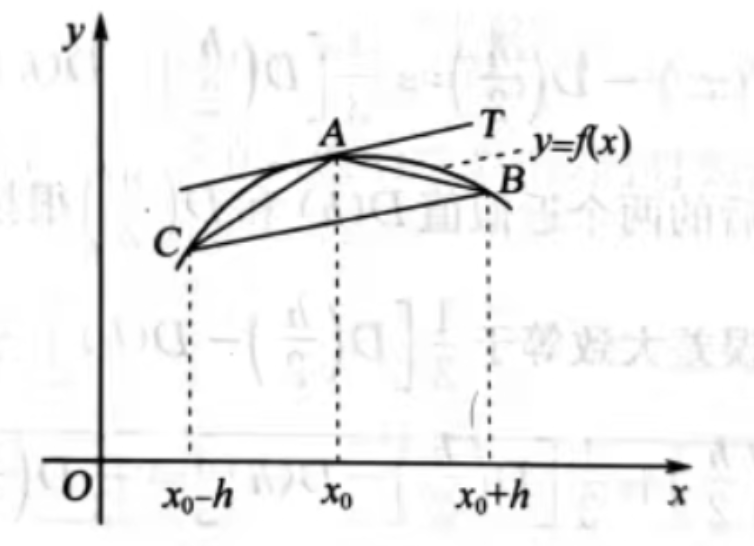
\includegraphics[width=6cm]{0.png}},{}]
 在如图所示的几何图形上,这三种差商分别表示弦 $AB,AC$ 和 $BC$ 的斜率 将这三条弦同过 $A$ 点的切线 $AT$ 相比较,一般地说,弦 $BC$ 的斜率更接近于切线 $AT$  的斜率 $f\left( x_{0} \right)$ ,因此就精度而言,第三个式子更为可取. 
 我们称
$D(h) = \dfrac{f\left( x_{0} + h \right) {-} f\left( x_{0} {-} h \right)}{2h}$为求 $f^{{\prime}}\left( x_{0} \right)$ 的中点公式.
现在来考察用中点公式 代替 $f^{{\prime}}\left( x_{0} \right)$ 所产生的截断误差 $f^{{\prime}}\left( x_{0} \right) {-} D(h)$ . 由泰 勒展开式有
\end{window}



$$\begin{aligned}
    f^{{\prime}}\left( x_{0} \right) {-} D(h) &= f^{{\prime}}\left( x_{0} \right) {-} \frac{1}{2h}\left\lbrack f\left( x_{0} + h \right) {-} f\left( x_{0} {-} h \right) \right\rbrack\\
    &= f^{{\prime}}\left( x_{0} \right) {-} \frac{1}{2h}\left\{\lbrack f\left( x_{0} \right) + hf^{{\prime}}\left( x_{0} \right) + \frac{1}{2}h^{2}f^{{\prime}{\prime}}\left( x_{0} \right)  +\frac{1}{6}h^{3}f^{{\prime}{\prime}{\prime}}\left( x_{0} + {\theta}_{1}h \right) \right\rbrack \\&{-} \left\lbrack f\left( x_{0} \right) {-} hf^{{\prime}}\left( x_{0} \right) \right.\left. \left. +\frac{1}{2}h^{2}f^{{\prime}{\prime}}\left( x_{0} \right) {-} \frac{1}{6}h^{3}f^{{\prime}{\prime}{\prime}}\left( x_{0} {-} {\theta}_{2}h \right) \right\rbrack \right\}\\
    &=-\frac{1}{12} h^{2}\left[f^{\prime \prime}\left(x_{0}+\theta_{1} h\right)+f^{\prime \prime}\left(x_{0}-\theta_{2} h\right)\right] \\
&=-\frac{1}{6} h^{2} f^{\prime \prime}\left(x_{0}+\theta h\right),
\end{aligned}$$
其中, $ \theta_{1}, \theta_{2} \in(0,1), \theta \in(-1,1) $.
从截断误差的角度来看,步长 $ h $ 越小,计算结果越精确. 但从舍入误差的角度看, 如果 $ h $ 越小, 则 $ f\left(x_{0}+h\right) $ 与 $ f\left(x_{0}-h\right) $ 越接近, 直接相减会造成有效数字的严重损失, 因此步长 $ h $ 不宜太小. %那怎样选取合适的步长呢? 可采用二分步长及事后误差估计法.

由以上讨论可知,对于中点公式,若以缩小步长 $h$ 来提高精度,那么只能适合于用解析式表示的函数,对于列表函数的求导,若要提高精度,还需另想别的方法.

对于列表函数 $y=f(x)$:
\begin{center}
\begin{tabular}{c|cccc}
$ x $ & $ x_{0} $ & $ x_{1} $ & $ \cdots $ & $ x_{n} $ \\
\hline$ y $ & $ y_{0} $ & $ y_{1} $ & $ \cdots $ & $ y_{n} $
\end{tabular}
\end{center}
应用插值原理, 可以建立插值多项式 $ p_{n}(x) $ 作为 $ f(x) $ 的近似. 由于多项式的求导比较容易, 因此可以取 $ p_{n}^{\prime}(x) $ 的值作为 $ f^{\prime}(x) $ 的近似值, 这样建立的数值公式
$$
f^{\prime}(x) \approx p_{n}^{\prime}(x)
$$
统称为\textbf{插值型求导公式}.

插值型求导公式 $ p_{n}^{\prime}(x) $ 的截断误差由插值余项
$$
f(x)-p_{n}(x)=\frac{f^{(n+1)}(\xi)}{(n+1)!} W_{n+1}(x)
$$
求导数得到. 因为
$$
\begin{array}{c}
\xi=\xi(x) \in\left(\min \left\{x, x_{0}, \cdots, x_{n}\right\}, \max \left\{x, x_{0}, \cdots, x_{n}\right\}\right), \\
W_{n+1}(x)=\left(x-x_{0}\right)\left(x-x_{1}\right) \cdots\left(x-x_{n}\right),
\end{array}
$$
于是 $ p_{n}^{\prime}(x) $ 的截断误差为
$$
f^{\prime}(x)-p_{n}^{\prime}(x)=\frac{f^{(n+1)}(\xi)}{(n+1)!} W_{n+1}^{\prime}(x)+\frac{W_{n+1}(x)}{(n+1)!} \frac{\mathrm{d}}{\mathrm{d} x} f^{(n+1)}(\xi) .
$$
上面的公式中, $ \xi $ 是 $ x $ 的未知函数, 很难对 $ \frac{\mathrm{d}}{\mathrm{d} x} f^{(n+1)}(\xi) $ 作进一步的估计. 若限定在某个节点 $ x_{k} $ 上求导数, 并注意到 $ W_{n+1}\left(x_{k}\right)=0 $, 此时 $ p^{\prime}{ }_{n}\left(x_{k}\right) $ 的截断误差表达式变得很简单, 即有
$$
f^{\prime}\left(x_{k}\right)-p_{n}^{\prime}\left(x_{k}\right)=\frac{f^{(n+1)}(\xi)}{(n+1)!} W_{n+1}^{\prime}\left(x_{k}\right)=\frac{f^{(n+1)}(\xi)}{(n+1)!} \prod_{\substack{j=0 \\ j \neq k}}^{n}\left(x_{k}-x_{j}\right) .
$$

由于以上的原因,下面仅考虑节点处的导数值.

(1) 两点公式

已知列表函数 $ y=f(x): $
\begin{tabular}{c|cc}
$ x $ & $ x_{0} $ & $ x_{1} $ \\
\hline$ y $ & $ f\left(x_{0}\right) $ & $ f\left(x_{1}\right) $
\end{tabular}
作一次插值多项式
$$
p_{1}(x)=\frac{x-x_{1}}{x_{0}-x_{1}} f\left(x_{0}\right)+\frac{x-x_{0}}{x_{1}-x_{0}} f\left(x_{1}\right) .
$$
对上式两端求导, 并记 $ h=x_{1}-x_{0} $, 则有
$$
p_{1}^{\prime}(x)=\frac{1}{h}\left[-f\left(x_{0}\right)+f\left(x_{1}\right)\right]
$$
于是有下列求导公式:
$$
p_{1}^{\prime}\left(x_{0}\right)=\frac{1}{h}\left[f\left(x_{1}\right)-f\left(x_{0}\right)\right], \quad p_{1}^{\prime}\left(x_{1}\right)=\frac{1}{h}\left[f\left(x_{1}\right)-f\left(x_{0}\right)\right],
$$

这与已介绍的向前差商与向后差商公式 是一致的. 而 $ p_{1}^{\prime}\left(x_{0}\right)=p_{1}^{\prime}\left(x_{1}\right) $ 是不奇怪的,因为 $ A, B $ 两点处的导数都以直线 $ A B $ 的斜率为近似值. 但它们的截断误差应该是不同的. 事实上, 有
$$
\begin{aligned}
f^{\prime}\left(x_{0}\right)-p_{1}^{\prime}\left(x_{0}\right)&=\frac{f^{\prime \prime}\left(\xi_{0}\right)}{2!} W_{2}^{\prime}\left(x_{0}\right)=\frac{f^{\prime \prime}\left(\xi_{0}\right)}{2}\left(x_{0}-x_{1}\right)=-\frac{h}{2} f^{\prime \prime}\left(\xi_{0}\right), \\
f^{\prime}\left(x_{1}\right)-p_{1}^{\prime}\left(x_{1}\right)&=\frac{f^{\prime \prime}\left(\xi_{1}\right)}{2!} W_{2}^{\prime}\left(x_{1}\right)=\frac{f^{\prime}\left(\xi_{1}\right)}{2}\left(x_{1}-x_{0}\right)=\frac{h}{2} f^{\prime \prime}\left(\xi_{1}\right),
\end{aligned}
$$
因此带余项的两点公式为
$$
\begin{aligned}
f^{\prime}\left(x_{0}\right)&=\frac{1}{h}\left[f\left(x_{1}\right)-f\left(x_{0}\right)\right]-\frac{h}{2} f^{\prime \prime}\left(\xi_{0}\right), \quad x_{0}<\xi_{0}<x_{1}, \\
f^{\prime}\left(x_{1}\right)&=\frac{1}{h}\left[f\left(x_{1}\right)-f\left(x_{0}\right)\right]+\frac{h}{2} f^{\prime \prime}\left(\xi_{1}\right), \quad x_{0}<\xi_{1}<x_{1} . \\
\end{aligned}
$$

(2) 三点公式

已知列表函数 $ y=f(x) $ :
\begin{tabular}{c|ccc}
$ x $ & $ x_{0} $ & $ x_{1} $ & $ x_{2} $ \\
\hline$ y $ & $ f\left(x_{0}\right) $ & $ f\left(x_{1}\right) $ & $ f\left(x_{2}\right) $
\end{tabular}
作 2 次插值多项式
$$
\begin{aligned}
p_{2}(x)= & \frac{\left(x-x_{1}\right)\left(x-x_{2}\right)}{\left(x_{0}-x_{1}\right)\left(x_{0}-x_{2}\right)} f\left(x_{0}\right)+\frac{\left(x-x_{0}\right)\left(x-x_{2}\right)}{\left(x_{1}-x_{0}\right)\left(x_{1}-x_{2}\right)} f\left(x_{1}\right)  +\frac{\left(x-x_{0}\right)\left(x-x_{1}\right)}{\left(x_{2}-x_{0}\right)\left(x_{2}-x_{1}\right)} f\left(x_{2}\right) .
\end{aligned}
$$
对 $ p_{2}(x) $ 求导, 得
$$
\begin{aligned}
p_{2}^{\prime}(x)= & \frac{2 x-x_{1}-x_{2}}{\left(x_{0}-x_{1}\right)\left(x_{0}-x_{2}\right)} f\left(x_{0}\right)+\frac{2 x-x_{0}-x_{2}}{\left(x_{1}-x_{0}\right)\left(x_{1}-x_{2}\right)} f\left(x_{1}\right)  +\frac{2 x-x_{0}-x_{1}}{\left(x_{2}-x_{0}\right)\left(x_{2}-x_{1}\right)} f\left(x_{2}\right),
\end{aligned}
$$
如果节点是等距的, 即 $ x_{2}-x_{1}=x_{1}-x_{0}=h $, 则有
$$
\begin{array}{l}
p_{2}^{\prime}\left(x_{0}\right)=\frac{1}{2 h}\left[-3 f\left(x_{0}\right)+4 f\left(x_{1}\right)-f\left(x_{2}\right)\right], \\
p_{2}^{\prime}\left(x_{1}\right)=\frac{1}{2 h}\left[-f\left(x_{0}\right)+f\left(x_{2}\right)\right], \\
p_{2}^{\prime}\left(x_{2}\right)=\frac{1}{2 h}\left[f\left(x_{0}\right)-4 f\left(x_{1}\right)+3 f\left(x_{2}\right)\right] .
\end{array}
$$
与两点公式同样的处理方法, 可求得 3 点公式的截断误差. 带余项的 3 点求导公式如下:
$$
\begin{array}{l}
f^{\prime}\left(x_{0}\right)=\frac{1}{2 h}\left[-3 f\left(x_{0}\right)+4 f\left(x_{1}\right)-f\left(x_{2}\right)\right]+\frac{h^{2}}{3} f^{\prime \prime \prime}\left(\xi_{0}\right), \quad x_{0}<\xi_{0}<x_{2}, \\
f^{\prime}\left(x_{1}\right)=\frac{1}{2 h}\left[-f\left(x_{0}\right)+f\left(x_{2}\right)\right]-\frac{h^{2}}{6} f^{\prime \prime \prime}\left(\xi_{1}\right), \quad x_{0}<\xi_{1}<x_{2}, \\
f^{\prime}\left(x_{2}\right)=\frac{1}{2 h}\left[f\left(x_{0}\right)-4 f\left(x_{1}\right)+3 f\left(x_{2}\right)\right]+\frac{h^{2}}{3} f^{\prime \prime \prime}\left(\xi_{2}\right), \quad x_{0}<\xi_{2}<x_{2} .
\end{array}
$$
$p_{2}^{\prime}\left(x_{1}\right)=\dfrac{1}{2 h}\left[-f\left(x_{0}\right)+f\left(x_{2}\right)\right]$ 即是我们所熟悉的中点公式, 它既达到了 3 点公式的精度, 截断误差是 $ O\left(h^{2}\right) $, 又只需用到 2 点处的函数值. 

将插值多项式 $ p_{n}(x) $ 作为 $ f(x) $ 的近似函数, 还可建立高阶导数数值微分公式
$$
f^{(k)}(x) \approx p_{n}^{(k)}(x), \quad k=1,2, \cdots .
$$
关于其截断误差, 有如下结论:
\begin{tcolorbox}[enhanced,colback=2,colframe=1,breakable,coltitle=green!25!black,title=定理]
 设 $ f(x) $ 在 $ [a, b] $ 上存在 $ n $ 阶导数, 在 $ (a, b) $ 上存在 $ (n+1) $ 阶导数,如果 $ a \leqslant x_{0}<x_{1}<\cdots<x_{n} \leqslant b, p_{n}(x) $ 为 $ f(x) $ 以 $ x_{0}, x_{1}, \cdots, x_{n} $ 为插值节点的 $ n $次插值多项式, 则对任何 $ x \in[a, b] $, 有
$$
f^{(k)}(x)-p_{n}^{(k)}(x)=\frac{f^{(n+1)}(\xi)}{(n-k+1)!}\left(x-x_{0}^{(k)}\right)\left(x-x_{1}^{(k)}\right) \cdots\left(x-x_{n-k}^{(k)}\right), \quad k=0,1,2, \cdots,
$$

其中, $ \xi \in(a, b) $ 且依赖于 $ k $ 和 $ x ; x_{i}<x_{i}^{(k)}<x_{i+k}, i=0,1, \cdots, n-k $.
\end{tcolorbox}






%  \begin{tcolorbox}[enhanced,colback=6,colframe=5,breakable,coltitle=green!25!black,title=My title]
% Upper part of my box.
% \tcblower
% Lower part of my box.
% \end{tcolorbox}

\subsection{Simpson 公式的余项另一种证明方法}
 设 $ f(x) $ 在区间 $ [a, b] $ 上有连续的四阶导数, 则辛普森公式的余项
$$
R_{S}=-\frac{(b-a)^{5}}{2880} f^{(4)}(\eta), a \leqslant \eta \leqslant b
$$

证: 辛普森公式的余项
$$
R_{S}=\frac{1}{3!} \int_{a}^{b} f^{(3)}(\xi)(x-a)\left(x-\frac{a+b}{2}\right)(x-b) \mathrm{d} x
$$
根据差商与导数的关系
$$
\begin{array}{c}
f\left[x, x_{0}, x_{1}, x_{2}\right]=\frac{f^{(3)}(\xi)}{3!} \\
\frac{\mathrm{d}}{\mathrm{d} x} f\left[x, x_{0}, x_{1}, x_{2}\right]=f\left[x, x, x_{0}, x_{1}, x_{2}\right]
\end{array}
$$
其中$x_{0}=a, x_{1}=\frac{a+b}{2}, x_{2}=b$, 取
$$
q(x)=\frac{1}{4}(x-a)^{2}(x-b)^{2}
$$
则
$$
q^{\prime}(x)=(x-a)\left(x-\frac{a+b}{2}\right)(x-b)
$$
于是
$$
\begin{aligned}
R_{S} & =\int_{a}^{b} f\left[x, x_{0}, x_{1}, x_{2}\right] q^{\prime}(x) \mathrm{d} x \\
& =\left.f\left[x, x_{0}, x_{1}, x_{2}\right] q(x)\right|_{a} ^{b}-\int_{a}^{b} q(x) \frac{\mathrm{d}}{\mathrm{d} x} f\left[x, x_{0}, x_{1}, x_{2}\right] \mathrm{d} x \\
& =-\frac{1}{4} \int_{a}^{b} f\left[x, x, x_{0}, x_{1}, x_{2}\right](x-a)^{2}(x-b)^{2} \mathrm{~d} x \\
& =-\frac{1}{4} f\left[\xi, \xi, x_{0}, x_{1}, x_{2}\right] \int_{a}^{b}(x-a)^{2}(x-b)^{2} \mathrm{~d} x \\
& =-\frac{1}{2880}(b-a)^{5} f^{(4)}(\eta)
\end{aligned}
$$



\section{常微分方程的数值解法练习题}
\subsection{课后习题}
   \begin{tcolorbox}[breakable,enhanced,arc=0mm,outer arc=0mm,
		boxrule=0pt,toprule=1pt,leftrule=0pt,bottomrule=1pt, rightrule=0pt,left=0.2cm,right=0.2cm,
		titlerule=0.5em,toptitle=0.1cm,bottomtitle=-0.1cm,top=0.2cm,
		colframe=white!10!biru,colback=white!90!biru,coltitle=white,
            coltext=black,title =2024-04, title style={white!10!biru}, before skip=8pt, after skip=8pt,before upper=\hspace{2em},
		fonttitle=\bfseries,fontupper=\normalsize]

 设有常微分方程初值问题如下:
$
\left\{\begin{array}{c}
y^{\prime}=f(x, y) \\
y\left(x_{0}\right)=y_{0}
\end{array}\right.
$

(1) 试推导数值求解公式 $ y_{i+1}=y_{i-1}+2 hf\left(x_{i}, y_{i}\right) $, 并验证公式的阶数

(2) 在初值问题中取 $ f(x, y)=2 x+3 y, x_{0}=0, y_{0}=2, $试用改进欧拉方法求 $ y(0.1) $ 的近似值, 并利用 (1) 中的公式求 $ y(0.2) $ 的近似值

(3) 求数值计算公式
$y_{i+1}=y_{i}+\frac{h}{2}\left[f\left(x_{i}, y_{i}\right)+f\left(x_{i}+\frac{h}{2}, y_{i}+\frac{h}{2} f\left(x_{i}, y_{i}\right)\right)\right]$的阶数
\tcblower
(1) %使用中心差商$\frac{1}{2h}[y(x_{i+1})-y(x_{i-1})]$替代方程 $y^{\prime}(x_i)=f(x_i, y(x_i))$中的导数项
中心差商近似导数:
$$
y'(x_i) \approx \frac{y(x_{i+1}) - y(x_{i-1})}{2h}
$$
将中心差商代入微分方程,得到:
$$
\frac{y(x_{i+1}) - y(x_{i-1})}{2h} = f(x_i, y(x_i))
$$
通过移项和整理,得到数值求解公式:
$$
y(x_{i+1}) = y(x_{i-1}) + 2hf(x_i, y(x_i))
$$
将 $ y(x_i) $ 用 $ y_i $ 表示,得到:
$$
y_{i+1} = y_{i-1} + 2hf(x_i, y_i)
$$
接下来我们验证公式的阶数.将 $ y = y(x) $ 在 $ x_{i+1} $ 和 $ x_{i-1} $ 点的函数值 $ y(x_{i+1}) $ 和 $ y(x_{i-1}) $ 展开为关于 $ x_i $ 点的泰勒级数:
$$
\begin{array}{l}
y(x_{i+1}) = y(x_i) + hy'(x_i) + \frac{h^2}{2} y''(x_i) + \frac{h^3}{6} y'''(\xi_1), \quad x_i < \xi_1 < x_{i+1} \\
y(x_{i-1}) = y(x_i) - hy'(x_i) + \frac{h^2}{2} y''(x_i) - \frac{h^3}{6} y'''(\xi_2), \quad x_{i-1} < \xi_2 < x_i
\end{array}
$$

将这两个式子相减,得:
$$
y(x_{i+1}) - y(x_{i-1}) = 2h y'(x_i) + \frac{h^3}{6} \left( y'''(\xi_1) + y'''(\xi_2) \right)=2h y'(x_i) + \frac{h^3}{3} y'''(\xi),\quad x_{i-1} < \xi < x_{i+1}
$$
因此有
$$
y(x_{i+1}) = y(x_{i-1}) + 2h y'(x_i) + O(h^3)
$$
因此,局部截断误差为:
$$y(x_{i+1})-y_{i+1}=[ y(x_{i-1}) + 2h y'(x_i) + O(h^3)]-[ y_{i-1} + 2hf(x_i, y_i)]=O(h^3)$$
故该公式为二阶方法.

(2)改进欧拉方法的公式为$\left\{\begin{array}{l}
    \widetilde{y}_{i+1}= y_i + h f(x_i, y_i)  \\
    y_{i+1} = y_i + \frac{h}{2} \left[ f(x_i, y_i) + f\left(x_{i + 1}, \widetilde{y}_{i+1} \right) \right]
\end{array}\right.$或写成如下形式:


$$y_{i+1} = y_i + \frac{h}{2} \left[ f(x_i, y_i) + f\left(x_{i + 1}, y_i + h f(x_i, y_i) \right) \right]
$$

给定初值问题:$\left\{
\begin{array}{l}
y' = 2x + 3y \\
y(0) = 2
\end{array}
\right.$我们需要用改进欧拉方法求  $y(0.1)$ 的近似值,取步长 $h = 0.1$.初始条件:$x_0 = 0, \quad y_0 = 2$, $\quad x_1 = x_0 + h = 0 + 0.1 = 0.1$, $f(x_0, y_0) = 2x_0 + 3y_0 = 2(0) + 3(2) = 6$
$$
\begin{array}{c}
      \widetilde{y}_{1} = y_0 + h f(x_0, y_0) = 2 + 0.1 \cdot 6 = 2 + 0.6 = 2.6 \\
     f(x_1, \widetilde{y}_{1}) = 2x_1 + 3\widetilde{y}_{1} = 2(0.1) + 3(2.6) = 0.2 + 7.8 = 8
\end{array}
$$
改进的 $y$ 值:
$$
   y_1 = y_0 + \frac{h}{2} \left[ f(x_0, y_0) + f(x_1, \widetilde{y}_{1}) \right] = 2 + \frac{0.1}{2} \left[ 6 + 8 \right] = 2 + 0.7 = 2.7
$$

因此,改进欧拉方法下 $ y(0.1) $ 的近似值为 2.7.

我们使用公式 $ y_{i+1} = y_{i-1} + 2hf(x_i, y_i) $ 来求 $ y(0.2) $ 的近似值.

%使用欧拉法计算 $ y_1 $:给定 $ x_0 = 0 $,$ y_0 = 2 $,步长 $ h = 0.1 $.

%$$y_1 = y_0 + h f(x_0, y_0)$$

%计算 $ f(x_0, y_0) $:$f(x_0, y_0) = 2x_0 + 3y_0 = 2 \cdot 0 + 3 \cdot 2 = 6$

%因此,$$y_1 = 2 + 0.1 \cdot 6 = 2 + 0.6 = 2.6$$

使用两步中点法计算 $ y_2 $:现在我们有两个初始点 $ y_0 = 2 $ 和 $ y_1 = 2.7 $.使用两步中点法公式来计算 $ y_2 $:
$$
y_2 = y_0 + 2hf(x_1, y_1)
$$
根据$x_1 = 0.1, \quad y_1 = 2.7$计算得
$$
f(x_1, y_1) = 2x_1 + 3y_1 = 2 \cdot 0.1 + 3 \cdot 2.7 = 0.2 +8.1 = 8.3
$$
因此,
$$
y_2 = y_0 + 2 \cdot 0.1 \cdot 8.3 = 2 + 1.66 = 3.66
$$
所以,使用两步中点法公式求得 $ y(0.2) $ 的近似值为 3.66.

(3)
对方程两边求导, 可得
$$
\begin{aligned}
 y^{\prime}(x)=&f(x, y), \quad y^{\prime \prime}(x)=\frac{\partial f(x, y(x))}{\partial x}+y^{\prime}(x) \frac{\partial f(x, y(x))}{\partial y}, \\
y^{\prime \prime \prime}(x)= & \frac{\partial^{2} f(x, y(x))}{\partial x^{2}}+y^{\prime}(x) \frac{\partial^{2} f(x, y(x))}{\partial x \partial y} \\
& +y^{\prime}(x)\left[\frac{\partial^{2} f(x, y(x))}{\partial x \partial y}+y^{\prime}(x) \frac{\partial^{2} f(x, y(x))}{\partial y^{2}}\right]+y^{\prime \prime}(x) \frac{\partial f(x, y(x))}{\partial y},
\end{aligned}
$$

则
$$
\begin{aligned}
R_{i+1}= & y\left(x_{i+1}\right)-\left[y\left(x_{i}\right)+\frac h2 f(x_i,y_i)+\frac h2 f\left(x_{i}+\frac{h}{2}, y\left(x_{i}\right)+\frac{h}{2} f\left(x_{i}, y\left(x_{i}\right)\right)\right)\right] \\
= & y\left(x_{i+1}\right)-y\left(x_{i}\right)-\frac h2 f(x_i,y_i)-\frac h2 f\left(x_{i}+\frac{h}{2}, y\left(x_{i}\right)+\frac{h}{2} y^{\prime}\left(x_{i}\right)\right) \\
= & h y^{\prime}\left(x_{i}\right)+\frac{h^{2}}{2} y^{\prime \prime}\left(x_{i}\right)+\frac{h^{3}}{6} y^{\prime \prime \prime}\left(x_{i}\right)+O\left(h^{4}\right)-\frac h2 f(x_i,y_i) \\
& -\frac h2\left\{f\left(x_{i}, y\left(x_{i}\right)\right)+\frac{h}{2} \frac{\partial f\left(x_{i}, y\left(x_{i}\right)\right)}{\partial x}+\frac{h}{2} y^{\prime}\left(x_{i}\right) \frac{\partial f\left(x_{i}, y\left(x_{i}\right)\right)}{\partial y}\right. \\
& +\frac{1}{2}\left[\frac{h^{2}}{4} \frac{\partial^{2} f\left(x_{i}, y\left(x_{i}\right)\right)}{\partial x^{2}}+\frac{h^{2}}{2} y^{\prime}\left(x_{i}\right) \frac{\partial^{2} f\left(x_{i}, y\left(x_{i}\right)\right)}{\partial x \partial y}\right.  \left.\left.+\left(\frac{h}{2} y^{\prime}\left(x_{i}\right)\right)^{2} \frac{\partial^{2} f\left(x_{i}, y\left(x_{i}\right)\right)}{\partial y^{2}}\right]+O\left(h^{3}\right)\right\} \\
= & \frac h2 y^{\prime}\left(x_{i}\right)+\frac{h^{2}}{2} y^{\prime \prime}\left(x_{i}\right)+\frac{h^{3}}{6} y^{\prime \prime \prime}\left(x_{i}\right)+O\left(h^{4}\right) \\
& -\frac h2\left\{y^{\prime}\left(x_{i}\right)+\frac{h}{2} y^{\prime \prime}\left(x_{i}\right)+\frac{h^{2}}{8}\left[y^{\prime \prime \prime}\left(x_{i}\right)-y^{\prime \prime}\left(x_{i}\right) \frac{\partial f\left(x_{i}, y\left(x_{i}\right)\right)}{\partial y}\right]+O\left(h^{3}\right)\right\} \\
= &\frac 14 h^2y^{\prime \prime}\left(x_{i}\right)+ \frac{5}{48}h^3 y^{\prime \prime \prime}\left(x_{i}\right)+\frac{1}{16}h^3 y^{\prime \prime}\left(x_{i}\right) \frac{\partial f\left(x_{i}, y\left(x_{i}\right)\right)}{\partial y}+O\left(h^{4}\right),
\end{aligned}
$$

所给求解公式是一个 一阶公式.

  \end{tcolorbox}


     \begin{tcolorbox}[breakable,enhanced,arc=0mm,outer arc=0mm,
		boxrule=0pt,toprule=1pt,leftrule=0pt,bottomrule=1pt, rightrule=0pt,left=0.2cm,right=0.2cm,
		titlerule=0.5em,toptitle=0.1cm,bottomtitle=-0.1cm,top=0.2cm,
		colframe=white!10!biru,colback=white!90!biru,coltitle=white,
            coltext=black,title =2024-04, title style={white!10!biru}, before skip=8pt, after skip=8pt,before upper=\hspace{2em},
		fonttitle=\bfseries,fontupper=\normalsize]
用梯形方法解初值问题 $ \left\{\begin{array}{c}y^{\prime}+y=0 \\ y(0)=1\end{array}\right. $ 证明其近似解为 $ y_{n}=\left(\frac{2-h}{2+h}\right)^{n} $, 并证明: 当 $ h \rightarrow 0 $ 时, 它收敛于原初始问题的精确解 $ y=e^{-x} $
\tcblower
梯形方法是一个数值解常微分方程的方法,其迭代格式为:
$$ y_{n+1} = y_n + \frac{h}{2}(f(x_n, y_n) + f(x_{n+1}, y_{n+1})) $$
其中,$ h $ 是步长,$ f(x, y) $ 是微分方程 $ y' = f(x, y) $ 中的右端函数.

对于给定的初值问题 $ \left\{\begin{array}{l}y^{\prime}+y=0 \\ y(0)=1\end{array}\right. $,我们有 $ f(x, y) = -y $.将其代入梯形方法的迭代格式中,得到:
$$ y_{n+1} = y_n + \frac{h}{2}(-y_n - y_{n+1}) $$
整理得到:$ y_{n+1} = \frac{2-h}{2+h}y_n $. 于是
$$
y_{n+1}=\left(\frac{2-h}{2+h}\right) y_{n}=\left(\frac{2-h}{2+h}\right)^{2} y_{n-1}=\cdots=\left(\frac{2-h}{2+h}\right)^{n+1} y_{0}
$$
因此,我们证明了 $ y_{n}=\left(\frac{2-h}{2+h}\right)^{n} $ 是给定初值问题的近似解.

%另一方面,对$\forall x>0$, 以 $h$ 为步长经过 $n$ 步运算可求得$y(x_n)$的近似值 $y_n$,所以$x=nh,n=\frac xh$.
因为 $ y_{0}=1 $, 故
$$
y_{n}=\left(\frac{2-h}{2+h}\right)^{n}
$$

对于给定的步长 $ h $,经过 $ n $ 步运算后,我们可以得到 $ y(x) $ 的近似值 $ y_n$.在每一步中,我们都会在 $ x $ 的位置上进行计算,因此总共进行 $ n $ 步运算后,我们得到的 $ x $ 的取值为 $ x = nh $.即 $ n=\dfrac{x}{h} $, 代入上式有:
$$
\begin{aligned}
y_{n}&=\left(\frac{2-h}{2+h}\right)^{\frac x  h} \\
\lim _{h \rightarrow 0} y_{n}&=\lim _{h \rightarrow 0}\left(\frac{2-h}{2+h}\right)^{\frac{x}{h}}=\lim _{h \rightarrow 0}\left(1-\frac{2 h}{2+h}\right)^{\frac{x}{h}} \\
&=\lim _{h \rightarrow 0}\left[\left(1-\frac{2 h}{2+h}\right)^{\frac{2+h}{2 h}}\right]^{\frac{2 h}{2+h}\cdot \frac{x}{h}}=\mathrm{e}^{-x}
\end{aligned}
$$
因此,当 $ h \rightarrow 0 $ 时,$ y_{n}=\left(\frac{2-h}{2+h}\right)^{n} $ 收敛于原初值问题的精确解 $ y=e^{-x} $.

  \end{tcolorbox}


     \begin{tcolorbox}[breakable,enhanced,arc=0mm,outer arc=0mm,
		boxrule=0pt,toprule=1pt,leftrule=0pt,bottomrule=1pt, rightrule=0pt,left=0.2cm,right=0.2cm,
		titlerule=0.5em,toptitle=0.1cm,bottomtitle=-0.1cm,top=0.2cm,
		colframe=white!10!biru,colback=white!90!biru,coltitle=white,
            coltext=black,title =2024-04, title style={white!10!biru}, before skip=8pt, after skip=8pt,before upper=\hspace{2em},
		fonttitle=\bfseries,fontupper=\normalsize]
 应用 Taylor 定理构建求解常微分方程初值问题 $ \left\{\begin{array}{l}y^{\prime}=-y^{2} \\ y(0)=1\end{array}\right. $ 的 2 阶近似求解方法
\tcblower

对于给定的初值问题 $ y'(x) = -y(x)^2 $,我们可以对 $ y(x) $ 进行 Taylor 展开:
$$
y(x_{i+1}) = y(x_i) + hy'(x_i) + \frac{h^2}{2}y''(x_i) + O(h^3)
$$

其中,$ h $ 是步长,$ y'(x_i) $ 和 $ y''(x_i) $ 是 $ y(x) $ 在 $ x_i $ 处的导数和二阶导数.

 已知 $ y'(x) = -y^2 $,所以有$y'(x_i) = -y^2(x_i)$.对 $ y'(x) $ 再求导得到$ y''(x) $:
$$
y''(x) = \frac{d}{dx}(-y^2) = -2y \cdot y'(x)
$$
将 $ y'(x) = -y^2 $ 代入上式得到:$y''(x) = -2y \cdot (-y^2) = 2y^3$.

利用 Taylor 展开式在$x_i$处展开:
$$
y(x_{i+1}) = y(x_i) + hy'(x_i) + \frac{h^2}{2}y''(x_i) + O(h^3)
$$

代入计算得到的 $ y'(x_i) $ 和 $ y''(x_i) $:
$$\begin{aligned}
    y(x_{i+1}) &= y(x_i) + h(-y^2(x_i)) + \frac{h^2}{2}(2y^3(x_i)) + O(h^3)\\&= y(x_i) - hy^2(x_i) + h^2y^3(x_i) + O(h^3)
\end{aligned}
$$

因此,二阶近似求解方法为:
$$
y_{i+1} = y_i - hy_i^2 + h^2y_i^3
$$

  \end{tcolorbox}


   \begin{tcolorbox}[breakable,enhanced,arc=0mm,outer arc=0mm,
		boxrule=0pt,toprule=1pt,leftrule=0pt,bottomrule=1pt, rightrule=0pt,left=0.2cm,right=0.2cm,
		titlerule=0.5em,toptitle=0.1cm,bottomtitle=-0.1cm,top=0.2cm,
		colframe=white!10!biru,colback=white!90!biru,coltitle=white,
            coltext=black,title =2024-04, title style={white!10!biru}, before skip=8pt, after skip=8pt,before upper=\hspace{2em},
		fonttitle=\bfseries,fontupper=\normalsize]
导出用 Euler 法求解 $ \left\{\begin{array}{l}y^{\prime}=\lambda y \\ y(0)=1\end{array} \quad(\lambda \neq 0)\right. $ 的公式, 并证明它收敛于初值问题的精确解.
\tcblower

令 $ x_i = i h $,根据欧拉法$ y_{i+1} = y_i + h f(x_i,y_i)$, 则 $ y_{i+1} = y_i + h y'(x_i) $. 对于 $ y'(x) = \lambda y $,有:
$$
y_{i+1} = y_i + h \lambda y_i = y_i (1 + h \lambda)
$$
初值条件为 $ y(0) = 1 $.因此,欧拉法的递推公式可以写成:$y_{i+1} = y_i (1 + h \lambda)$.

我们从初始值 $ y_0 = 1 $ 开始,逐步计算 $ y_1, y_2, \ldots $,可以得到一般公式:
$$
\begin{array}{l}
       y_1 = y_0 (1 + h \lambda) = 1 \cdot (1 + h \lambda)\\
      y_2 = y_1 (1 + h \lambda) = (1 + h \lambda)^2\\
      \cdots\cdots\\
      y_n = (1 + h \lambda)^n
\end{array}
$$

而易知初值问题的精确解为:$y(x) = e^{\lambda x}$, 
%在 $ x = nh $ 处的精确解为:
%$$
%y(nh) = e^{\lambda nh} = \left(e^{\lambda h}\right)^n
%$$
为了证明欧拉法求解的数值解 $ y_n = (1 + h \lambda)^n $ 收敛于精确解 $y(x) = e^{\lambda x}$,我们需要分析 $ (1 + h \lambda)^n $ 和 $ \left(e^{\lambda x}\right)$ 之间的关系.由于$ x = nh $,
%对于给定的步长 $ h $,经过 $ n $ 步运算后,我们可以得到 $ y(x) $ 的近似值 $ y_n$.在每一步中,我们都会在 $ x $ 的位置上进行计算,因此总共进行 $ n $ 步运算后,我们得到的 $ x $ 的取值为 $ x = nh $.即 $ n=\dfrac{x}{h} $, 代入上式有:
利用指数函数的定义,我们知道当 $ h \to 0 $ 时,有:
$$
\lim_{h\to 0}\left(1 + \lambda h \right)^n =\lim_{h\to 0}\left(1 + \lambda h \right)^{\frac{1}{\lambda h}\cdot \lambda h\cdot \frac{x}{h}}= \lim_{h\to 0}\left(1 + \lambda h \right)^{\frac{1}{\lambda h}\cdot \lambda x}= e^{\lambda x} 
$$

因此,当步长 $ h \to 0 $ (即 $ n \to \infty $)时,欧拉法的数值解 $ y_n = (1 + h \lambda)^n $ 收敛于精确解 $ y(x) = e^{\lambda x} $.


  \end{tcolorbox}

%1. Find the exact solution of the initial value problem $u^{{\prime}} = {-} u^{2},u(0) = 1,$ and compare it to the approximate solutions obtained by successive approximations according to Corollary 10.6. Compute the third iterate $u_{2}$ and compare the exact error $u {-} u_{2}$ to the a posteriori error estimate from Corollary 10.6.

%2. Show that the midpoint methpd for the solution of initial value problem $y_{n + 1} = y_{n {-} 1} + 2hf\left( x_{n},y_{n} \right)$ is convergent of order 2

%3. Using the Taylor expansion to construct the approximation method for the initial value problem $\left\{\begin{array}{l} y^{{\prime}} = {-} y^{2} \\ y(0) = 1 \end{array} \right.$ such that the method is convergent of order 2

%4. Using the trapezoidal (梯形) method to solve the initial value problem $\left\{\begin{matrix} y^{{\prime}} + y = 0 \\ y(0) = 1 \end{matrix} \right.$ ,show that the aproximation solution is $y_{n} = {\left( \frac{2 {-} h}{2 + h} \right)}^{n}$ and $\left\{y_{n} \right\}$ is convergent to the accurate solution $y = e^{{-}x}$ as $h {\rightarrow} 0$
\subsection{补充习题}


  \begin{tcolorbox}[enhanced,colback=8,colframe=7,breakable,coltitle=green!25!black,title=2024]
证明中点公式
$$
y_{n+1}=y_{n-1}+2 h f\left(x_{n}, y_{n}\right)
$$
是二阶的, 并给出其局部截断误差.
\tcblower
 考虑对应的离散关系式
$$
y\left(x_{n+1}\right) \approx y\left(x_{n-1}\right)+2 h y^{\prime}\left(x_{n}\right)
$$
泰勒展开有
$$
y\left(x_{n-1}\right)=y\left(x_{n}\right)-h y^{\prime}\left(x_{n}\right)+\frac{h^{2}}{2} y^{\prime \prime}\left(x_{n}\right)-\frac{h^{3}}{6} y^{\prime \prime \prime}\left(x_{n}\right)+O\left(h^{4}\right)
$$
代入离散关系式右端, 并记所得结果为 $ y_{n+1}^{*} $, 则有
$$
y_{n+1}^{*}=y\left(x_{n}\right)+h y^{\prime}\left(x_{n}\right)+\frac{h^{2}}{2} y^{\prime \prime}\left(x_{n}\right)-\frac{h^{3}}{6} y^{\prime \prime \prime}\left(x_{n}\right)+O\left(h^{4}\right)
$$
而
$$
y\left(x_{n+1}\right)=y\left(x_{n}\right)+h y^{\prime}\left(x_{n}\right)+\frac{h^{2}}{2} y^{\prime \prime}\left(x_{n}\right)+\frac{h^{3}}{6} y^{\prime \prime \prime}\left(x_{n}\right)+O\left(h^{4}\right)
$$
故局部截断误差
$$
\begin{aligned}
y\left(x_{n+1}\right)-y_{n+1}^{*} & =\left(\frac{1}{6}+\frac{1}{6}\right) h^{3} y^{\prime \prime \prime}\left(x_{n}\right)+O\left(h^{4}\right) \\
& = \frac{h^{3}}{3} y^{\prime \prime \prime}\left(x_{n}\right)+O\left(h^{4}\right)
\end{aligned}
$$
可见中点方法是二阶的.

 \end{tcolorbox}


   \begin{tcolorbox}[enhanced,colback=8,colframe=7,breakable,coltitle=green!25!black,title=2024]
给定常微分方程初值问题:
$
\left\{\begin{array}{l}
y^{\prime}=-y, \quad 0<x \leqslant a, \\
y(0)=1,
\end{array}\right.
$
取正整数 $ n $, 并记 $ h=\frac a n, x_{i}=i h, 0 \leqslant i \leqslant n $. 证明: 用梯形公式求解该初值问题所得的数值解为
$$
y_{i}=\left(\frac{2-h}{2+h}\right)^{i}
$$
且当 $ h \rightarrow 0 $ 时, $ y_{n} $ 收敛于 $ y(a) $.
 \tcblower
 梯形公式应用于方程有
$$
y_{i+1}=y_{i}+\frac{h}{2}\left(-y_{i}-y_{i+1}\right)
$$

即有
$$
\begin{array}{c}
\left(1+\frac{h}{2}\right) y_{i+1}=\left(1-\frac{h}{2}\right) y_{i} \\
y_{i+1}=\frac{2-h}{2+h} y_{i}=\left(\frac{2-h}{2+h}\right)^{2} y_{i-1}=\left(\frac{2-h}{2+h}\right)^{i+1} y_{0},
\end{array}
$$

所以
$$
y_{i}=\left(\frac{2-h}{2+h}\right)^{i}, \quad i=1,2, \cdots .
$$

当 $ h \rightarrow 0 $ 时, $ n \rightarrow \infty $, 我们有
$$
\begin{aligned}
\lim _{n \rightarrow \infty} y_{n} & =\lim _{n \rightarrow \infty}\left(\frac{2-h}{2+h}\right)^{n}=\lim _{h \rightarrow 0}\left(\frac{1-\frac{h}{2}}{1+\frac{h}{2}}\right)^{\frac{a}{h}} \\
& =\lim _{h \rightarrow 0} \frac{\left(1-\frac{h}{2}\right)^{-\frac{2}{h}\left(-\frac{a}{2}\right)}}{\left(1+\frac{h}{2}\right)^{\frac{2}{h}\left(\frac{a}{2}\right)}}=\frac{\mathrm{e}^{-\frac{a}{2}}}{\mathrm{e}^{\frac{a}{2}}}=\mathrm{e}^{-a},
\end{aligned}
$$

而由方程知解析解为 $ y=\mathrm{e}^{-x} $, 则 $ y(a)=\mathrm{e}^{-a} $, 所以
$$
\lim _{h \rightarrow 0} y_{n}=y(a) .
$$
 \end{tcolorbox}


  \begin{tcolorbox}[enhanced,colback=8,colframe=7,breakable,coltitle=green!25!black,title=2024]
 利用欧拉方法解初值问题
$
\left\{\begin{array}{l}
y^{\prime}=a x+b \\
y(0)=0
\end{array}\right.
$
其中 $ a, b $ 是常数. 求证其截断误差 $ y\left(x_{i}\right)-y_{i}=\frac{1}{2} a i h^{2} $.
\tcblower
% 对欧拉法, 将 $ y\left(x_{i+1}\right) $ 在 $ x_{i} $ 处进行泰勒展开,计算局部截断误差 $ y\left(x_{i+1}\right)-y_{i+1} $.

 初值问题的精确解为 $ y(x)=\frac{1}{2} a x^{2}+b x $.
因为 $ x_{i}=i h $, 所以应用欧拉方法得
$$
\begin{aligned}
y_{i+1} & =y_{i}+h f\left(x_{i}, y_{i}\right)=y_{i}+h\left(a x_{i}+b\right) =y_{i}+a i h^{2}+b h
\end{aligned}
$$
逐次利用上式得
$$
\begin{array}{c}
y_{i}=y_{i-1}+(i-1) a h^{2}+b h \\
\ldots \ldots \\
y_{2}=y_{1}+2 a h^{2}+b h \\
y_{1}=y_{0}+a h^{2}+b h
\end{array}
$$
又 $ y_{0}=0 $, 故
$$
y_{i}=y_{0}+a \frac{i(i-1)}{2} h^{2}+i b h=\frac{a i(i-1)}{2} h^{2}+b i h
$$
又因为
$$
y\left(x_{i}\right)=\frac{1}{2} a x_{i}^{2}+b x_{i}=\frac{1}{2} a i^{2} h^{2}+b i h
$$
所以截断误差
$$
R_{i}=y\left(x_{i}\right)-y_{i}=\frac{1}{2} a_{i h}^{2}
$$
 \end{tcolorbox}

\begin{tcolorbox}[enhanced,colback=8,colframe=7,breakable,coltitle=green!25!black,title=2024]

 求证:改进的 Euler 格式能精确地解初值问题
$
\left\{\begin{array}{l}
y^{\prime}=a x+b, \\
y(0)=0,
\end{array}\right.
$
其中 $ a, b $ 是常数.
\tcblower
容易求出初值问题的真解
$$
y(x)=\frac{1}{2} a x^{2}+b x .
$$
应用改进的 Euler 格式得
$$
\begin{aligned}
y_{n+1} & =y_{n}+\frac{h}{2}\left(f\left(x_{n}, y_{n}\right)+f\left(x_{n}+h, y_{n}+h f\left(x_{n}, y_{n}\right)\right)\right) \\
& =y_{n}+\frac{h}{2}\left(a x_{n}+b+a\left(x_{n}+h\right)+b\right)=y_{n}+a\left(n+\frac{1}{2}\right) h^{2}+b h .
\end{aligned}
$$
逐次利用上式得
$$
\begin{array}{c}
y_{n}=y_{n-1}+a\left(n-\frac{1}{2}\right) h^{2}+b h, \\
\cdots \cdots \\
y_{2}=y_{1}+a\left(2-\frac{1}{2}\right) h^{2}+b h, \\
y_{1}=y_{0}+a\left(1-\frac{1}{2}\right) h^{2}+b h,
\end{array}
$$
所以
$$
y_{n}=y_{0}+a\left(\frac{n(n+1)}{2}-\frac{n}{2}\right) h^{2}+n b h=\frac{1}{2} a n^{2} h^{2}+n b h .
$$
注意到
$$
y\left(x_{n}\right)=\frac{1}{2} a x_{n}^{2}+b x_{n}=\frac{1}{2} a n^{2} h^{2}+b n h,
$$
显然
$y_{n}=y\left(x_{n}\right),$ 即改进的 Euler 法能精确地解该初值问题.
 \end{tcolorbox}

 
\begin{tcolorbox}[enhanced,colback=8,colframe=7,breakable,coltitle=green!25!black,title=2024]
 对于初值问题
$
\left\{\begin{array}{l}
y^{\prime}+y=0, x>0 \\
y(0)=1
\end{array}\right.
$
试证明用改进欧拉方法所求近似解为 $ y_{i}=\left(1-h+h^{2} / 2\right)^{i}(i=0,1,2, \cdots) $.
\tcblower
 改进的欧拉法表达式为
$$
\left\{\begin{array}{l}
\bar{y}_{i+1}=y_{i}+h f\left(x_{i}, y_{i}\right) \\
y_{i+1}=y_{i}+\frac{h}{2}\left[f\left(x_{i}, y_{i}\right)+f\left(x_{i+1}, \bar{y}_{i+1}\right)\right]
\end{array}\right.
$$
将 $ f(x, y)=-y $ 代入得
$$
\begin{aligned}
y_{i+1}&=y_{i}+\frac{h}{2}\left[f\left(x_{i}, y_{i}\right)+\right.\left.f\left(x_{i+1}, \bar{y}_{i+1}\right)\right]\\&=y_{i}+\frac{h}{2}\left[\left(-y_{i}\right)-(1-h) y_{i}\right]=\left(1-h+\frac{h^{2}}{2}\right) y_{i} \\
&=\cdots=\left(1-h+\frac{h^{2}}{2}\right)^{i+1} y_{0}=\left(1-h+\frac{h^{2}}{2}\right)^{i+1}
\end{aligned}
$$
所以可得 $ y_{i}=\left(1-h+\frac{h^{2}}{2}\right)^{i}(i=0,1,2, \cdots) $.
\end{tcolorbox}
  \begin{tcolorbox}[enhanced,colback=8,colframe=7,breakable,coltitle=green!25!black,title=2024]
 给定常微分方程初值问题:
$
\left\{\begin{array}{l}
y^{\prime}=f(x, y), \quad a<x \leqslant b, \\
y(a)=\eta,
\end{array}\right.
$
取正整数 $ n $, 并记 $ h=(b-a) / n, x_{i}=a+i h, 0 \leqslant i \leqslant n $. 试分析求解公式
$$
y_{i+1}=y_{i}+h f\left(x_{i}+\frac{h}{2}, y_{i}+\frac{h}{2} f\left(x_{i}, y_{i}\right)\right)
$$
的局部截断误差, 并指出它是一个几阶的公式.
 \tcblower

 对方程两边求导, 可得
$$
\begin{aligned}
& y^{\prime}(x)=f(x, y), \quad y^{\prime \prime}(x)=\frac{\partial f(x, y(x))}{\partial x}+y^{\prime}(x) \frac{\partial f(x, y(x))}{\partial y}, \\
y^{\prime \prime \prime}(x)= & \frac{\partial^{2} f(x, y(x))}{\partial x^{2}}+y^{\prime}(x) \frac{\partial^{2} f(x, y(x))}{\partial x \partial y} \\
& +y^{\prime}(x)\left[\frac{\partial^{2} f(x, y(x))}{\partial x \partial y}+y^{\prime}(x) \frac{\partial^{2} f(x, y(x))}{\partial y^{2}}\right]+y^{\prime \prime}(x) \frac{\partial f(x, y(x))}{\partial y},
\end{aligned}
$$
则
$$
\begin{aligned}
R_{i+1}= & y\left(x_{i+1}\right)-\left[y\left(x_{i}\right)+h f\left(x_{i}+\frac{h}{2}, y\left(x_{i}\right)+\frac{h}{2} f\left(x_{i}, y\left(x_{i}\right)\right)\right)\right] \\
= & y\left(x_{i+1}\right)-y\left(x_{i}\right)-h f\left(x_{i}+\frac{h}{2}, y\left(x_{i}\right)+\frac{h}{2} y^{\prime}\left(x_{i}\right)\right) \\
= & h y^{\prime}\left(x_{i}\right)+\frac{h^{2}}{2} y^{\prime \prime}\left(x_{i}\right)+\frac{h^{3}}{6} y^{\prime \prime \prime}\left(x_{i}\right)+O\left(h^{4}\right) \\
& -h\left\{f\left(x_{i}, y\left(x_{i}\right)\right)+\frac{h}{2} \frac{\partial f\left(x_{i}, y\left(x_{i}\right)\right)}{\partial x}+\frac{h}{2} y^{\prime}\left(x_{i}\right) \frac{\partial f\left(x_{i}, y\left(x_{i}\right)\right)}{\partial y}\right. \\
& +\frac{1}{2}\left[\frac{h^{2}}{4} \frac{\partial^{2} f\left(x_{i}, y\left(x_{i}\right)\right)}{\partial x^{2}}+\frac{h^{2}}{2} y^{\prime}\left(x_{i}\right) \frac{\partial^{2} f\left(x_{i}, y\left(x_{i}\right)\right)}{\partial x \partial y}\right. \\
& \left.\left.+\left(\frac{h}{2} y^{\prime}\left(x_{i}\right)\right)^{2} \frac{\partial^{2} f\left(x_{i}, y\left(x_{i}\right)\right)}{\partial y^{2}}\right]+O\left(h^{3}\right)\right\} \\
= & h y^{\prime}\left(x_{i}\right)+\frac{h^{2}}{2} y^{\prime \prime}\left(x_{i}\right)+\frac{h^{3}}{6} y^{\prime \prime \prime}\left(x_{i}\right)+O\left(h^{4}\right) \\
& -h\left\{y^{\prime}\left(x_{i}\right)+\frac{h}{2} y^{\prime \prime}\left(x_{i}\right)+\frac{h^{2}}{8}\left[y^{\prime \prime \prime}\left(x_{i}\right)-y^{\prime \prime}\left(x_{i}\right) \frac{\partial f\left(x_{i}, y\left(x_{i}\right)\right)}{\partial y}\right]+O\left(h^{3}\right)\right\} \\
= & h^{3}\left[\frac{1}{24} y^{\prime \prime \prime}\left(x_{i}\right)+\frac{1}{8} y^{\prime \prime}\left(x_{i}\right) \frac{\partial f\left(x_{i}, y\left(x_{i}\right)\right)}{\partial y}\right]+O\left(h^{4}\right),
\end{aligned}
$$
所给求解公式是一个 2 阶公式.
 \end{tcolorbox}


    \begin{tcolorbox}[enhanced,colback=8,colframe=7,breakable,coltitle=green!25!black,title=2024]
 已知微分方程初值问题 $ y^{\prime}=x+y-1, y(0)=1 $.
 
(1) 取步长为 $ h=0.1 $, 试用 Euler 方法计算在 $ x=0.4 $ 处的近似值;

(2) 试用 Taylor 展开估计改进 Euler 方法的局部截断误差.
 \tcblower

 (1) 由题意可知, Euler 方法为
$$
y_{n+1}=y_{n}+h f\left(x_{n}, y_{n}\right)=y_{n}+h\left(x_{n}+y_{n}-1\right), \quad n=0,1,2, \cdots
$$
步长为 $ h=0.1 $, 初值 $ y(0)=1 $, 计算结果为
$$
\begin{array}{l}
y_{1}=y_{0}+0.1\left(x_{0}+y_{0}-1\right)=1 \\
y_{2}=y_{1}+0.1\left(x_{1}+y_{1}-1\right)=1.01 \\
y_{3}=y_{2}+0.1\left(x_{2}+y_{2}-1\right)=1.031 \\
y_{4}=y_{3}+0.1\left(x_{3}+y_{3}-1\right)=1.0641
\end{array}
$$
因此在 $ x=0.4 $ 处的近似值为 1.0641 .


(2) 由改进 Euler 方法的局部截断误差
$$
\begin{aligned}
R_{n+1} & =y\left(x_{n+1}\right)-y\left(x_{n}\right)-\frac{h}{2}\left[f\left(x_{n}, y_{n}\right)+f\left(x_{n+1}, y_{n+1}\right)\right] \\
& =y\left(x_{n+1}\right)-y\left(x_{n}\right)-\frac{h}{2}\left[y^{\prime}\left(x_{n}\right)+y^{\prime}\left(x_{n+1}\right)\right]
\end{aligned}
$$
又由
$$
\begin{array}{l}
y\left(x_{n+1}\right)=y\left(x_{n}\right)+h y^{\prime}\left(x_{n}\right)+\frac{h^{2}}{2} y^{\prime \prime}\left(x_{n}\right)+\frac{h^{3}}{3!} y^{\prime \prime \prime}\left(x_{n}\right)+\cdots \\
y^{\prime}\left(x_{n+1}\right)=y^{\prime}\left(x_{n}\right)+h y^{\prime \prime}\left(x_{n}\right)+\frac{h^{2}}{2} y^{\prime \prime \prime}\left(x_{n}\right)+\cdots
\end{array}
$$
整理得到
$$
R_{n+1}=\frac{h^{3}}{3!} y^{\prime \prime \prime}\left(x_{n}\right)-\frac{h}{2}\left[\frac{h^{2}}{2} y^{\prime \prime \prime}\left(x_{n}\right)+\cdots\right]=-\frac{h^{3}}{12} y^{\prime \prime \prime}\left(x_{n}\right)+O\left(h^{4}\right)
$$
所以改进 Euler 方法是 2 阶的, 其局部误差主项为 $ -\frac{h^{3}}{12} y^{\prime \prime \prime}\left(x_{n}\right) $.
 \end{tcolorbox}


    \begin{tcolorbox}[enhanced,colback=8,colframe=7,breakable,coltitle=green!25!black,title=2024]
 已知微分方程初值问题 $ y^{\prime}=e^{-x-y}, y(0)=0 $.

(1) 取步长为 $ h=0.1 $, 试用改进 Euler 方法计算在 $ x=0.3 $ 处的近似值;

(2) 试用 Taylor 展开估计改进 Euler 方法的局部截断误差.
 \tcblower
 (1) 由题意可知, $ f(x, y)=e^{-x-y} $, 步长为 $ h=0.1 $, 因此改进 Euler 方法,
$$
\begin{array}{c}
\bar{y}_{n+1}=y_{n}+h f\left(x_{n}, y_{n}\right)=y_{n}+0.1 e^{-x_{n}-y_{n}} \\
y_{n+1}=y_{n}+\frac{h}{2}\left(f\left(x_{n}, y_{n}\right)+f\left(x_{n+1}, \bar{y}_{n+1}\right)\right)=y_{n}+0.05\left(e^{-x_{n}-y_{n}}+e^{-x_{n+1}-\bar{y}_{n+1}}\right) \\
n=0,1,2, \cdots
\end{array}
$$
由初值 $ y(0)=0 $, 计算可得
$$
\begin{array}{l}
\left\{\begin{array}{l}
\bar{y}_{1}=y_{0}+0.1 e^{-x_{0}-y_{0}}=0.1 \\
y_{1}=y_{0}+0.05\left(e^{-x_{0}-y_{0}}+e^{-x_{1}-\bar{y}_{1}}\right) \approx 0.0952
\end{array}\right. \\
\left\{\begin{array}{l}
\bar{y}_{2}=y_{1}+0.1 e^{-x_{1}-y_{1}} \approx 0.1775 \\
y_{2}=y_{1}+0.05\left(e^{-x_{1}-y_{1}}+e^{-x_{2}-\bar{y}_{2}}\right) \approx 0.1706
\end{array}\right. \\
\left\{\begin{array}{l}
\bar{y}_{3}=y_{2}+0.1 e^{-x_{2}-y_{2}} \approx 0.2396 \\
y_{3}=y_{2}+0.05\left(e^{-x_{2}-y_{2}}+e^{-x_{3}-\bar{y}_{3}}\right) \approx 0.2343
\end{array}\right. \\
\end{array}
$$
因此计算在 $ x=0.3 $ 处的近似值 $ y_{3} \approx 0.2343 $.

(2) 由改进 Euler 方法格式
$$
\left\{\begin{array}{ll}
y_{n+1}=y_{n}+\frac{h}{2}\left[k_{1}+k_{2}\right], \\
k_{1}=f\left(x_{n}, y_{n}\right), & \\
k_{2}=f\left(x_{n}+h, y_{n}+h k_{1}\right), &
\end{array}\right.
$$
这里 $ k_{1}=f\left(x_{n}, y_{n}\right)=y^{\prime}\left(x_{n}\right) $. 由局部截断误差, 假设 $ y^{\prime}\left(x_{n}\right)=y_{n} $, 且
$$
y^{\prime \prime}\left(x_{n}\right)=f_{x}^{\prime}\left(x_{n}, y_{n}\right)+f_{y}^{\prime}\left(x_{n}, y_{n}\right) y^{\prime}\left(x_{n}\right)=f_{x}^{\prime}\left(x_{n}, y_{n}\right)+f_{y}^{\prime}\left(x_{n}, y_{n}\right) k_{1}
$$
由 Taylor 展开
$$
\begin{aligned}
k_{2}=&f\left(x_{n}+h, y_{n}+h k_{1}\right)=f\left(x_{n}, y_{n}\right)+h f_{x}^{\prime}\left(x_{n}, y_{n}\right)+h k_{1} f_{y}^{\prime}\left(x_{n}, y_{n}\right)\\
& +\frac{1}{2!}\left[h^{2} f_{x x}^{\prime \prime}\left(x_{n}, y_{n}\right)+2 h^{2} k_{1} f_{x y}^{\prime \prime}\left(x_{n}, y_{n}\right)+h^{2} k_{1}^{2} f_{y y}^{\prime \prime}\left(x_{n}, y_{n}\right)\right]+O\left(h^{3}\right) \\
= & y^{\prime}\left(x_{n}\right)+h y^{\prime \prime}\left(x_{n}\right)+\frac{h^{2}}{2!}\left[f_{x x}^{\prime \prime}\left(x_{n}, y_{n}\right)+2 k_{1} f_{x y}^{\prime \prime}\left(x_{n}, y_{n}\right)+k_{1}^{2} f_{y y}^{\prime \prime}\left(x_{n}, y_{n}\right)\right]+O\left(h^{3}\right)
\end{aligned}
$$
分别代入 $y_{n+1}=  y_{n}+\frac{h}{2}\left[k_{1}+k_{2}\right]$,整理得
$$
\begin{aligned}
y_{n+1}=  y_{n}+h y^{\prime}\left(x_{n}\right)+\frac{h^{2}}{2} y^{\prime \prime}\left(x_{n}\right)+\frac{h^{3}}{4}\left[f_{x x}^{\prime \prime}\left(x_{n}, y_{n}\right)\right.  \left.+2 k_{1} f_{x y}^{\prime \prime}\left(x_{n}, y_{n}\right)+k_{1}^{2} f_{y y}^{\prime \prime}\left(x_{n}, y_{n}\right)\right]+O\left(h^{4}\right)
\end{aligned}
$$

又由 $ y\left(x_{n+1}\right)=y\left(x_{n}+h\right)=y\left(x_{n}\right)+h y^{\prime}\left(x_{n}\right)+\frac{h^{2}}{2!} y^{\prime \prime}\left(x_{n}\right)+\frac{h^{3}}{3!} y^{\prime \prime \prime}\left(x_{n}\right)+O\left(h^{4}\right) $, 因此整理后局部截断误差
$$
\begin{aligned}
y\left(x_{n+1}\right)-y\left(x_{n}\right) \approx & \frac{h^{3}}{4}\left[f_{x x}^{\prime \prime}\left(x_{n}, y_{n}\right)+2 k_{1} f_{x y}^{\prime \prime}\left(x_{n}, y_{n}\right)+k_{1}^{2} f_{y y}^{\prime \prime}\left(x_{n}, y_{n}\right)\right]-\frac{h^{3}}{3!} y^{\prime \prime \prime}\left(x_{n}\right)=O\left(h^{3}\right)
\end{aligned}
$$
 \end{tcolorbox}
 
\begin{tcolorbox}[enhanced,colback=8,colframe=7,breakable,coltitle=green!25!black,title=2024]
对于求解初值问题
$
\left\{\begin{array}{l}
y^{\prime}=f(x, y) \\
y\left(x_{0}\right)=y_{0}
\end{array}\right.
$
的数值方法 $ y_{i+1}=y_{i}+\frac{h}{3}\left[f\left(x_{i}, y_{i}\right)+2 f\left(x_{i+1}, y_{i+1}\right)\right] $, 试求其局部截断误差和阶数.

%分析: 将 $ y\left(x_{i+1}\right) $ 在 $ x_{i} $ 处进行泰勒展开,可求得该方法的局部截断误差和阶数. 再将该方法应用于模型方程, 求得其绝对稳定应满足的条件.
\tcblower
 当 $ y_{i}=y\left(x_{i}\right) $ 时, 将 $ y\left(x_{i+1}\right) $ 在 $ x_{i} $ 处泰勒展开得
$$
y\left(x_{i+1}\right)=y\left(x_{i}\right)+y^{\prime}\left(x_{i}\right) h+\frac{1}{2!} y^{\prime \prime}\left(x_{i}\right) h^{2}+O\left(h^{3}\right)
$$
将该初值问题的数值解 $ y_{i+1} $ 在 $ x_{i} $ 处泰勒展开:
因为 $ f\left(x_{i+1}, y_{i+1}\right)=y^{\prime}\left(x_{i+1}\right)=y^{\prime}\left(x_{i}\right)+y^{\prime \prime}\left(x_{i}\right) h+O\left(h^{2}\right) $, 所以
$$
\begin{aligned}
y_{i+1} & =y_{i}+\frac{h}{3}\left[f\left(x_{i}, y_{i}\right)+2 f\left(x_{i+1}, y_{i+1}\right)\right] \\
& =y\left(x_{i}\right)+\frac{h}{3}\left\{y^{\prime}\left(x_{i}\right)+2\left[y^{\prime}\left(x_{i}\right)+y^{\prime \prime}\left(x_{i}\right) h+O\left(h^{2}\right)\right]\right\}\\
&=y\left(x_{i}\right)+\frac{h}{3}\left[y^{\prime}\left(x_{i}\right)+2 y^{\prime}\left(x_{i}\right)+2 h y^{\prime \prime}\left(x_{i}\right)+O\left(h^{3}\right)\right]
\end{aligned}
$$
于是得局部截断误差
$$
R_{i+1}  =y\left(x_{i+1}\right)-y_{i+1}  =-\frac{1}{6} h^{2} y^{\prime \prime}\left(x_{i}\right)+O\left(h^{3}\right)
$$
即 $ R_{i+1}=O\left(h^{2}\right) $, 因此该方法是一阶的.
\end{tcolorbox}


  \begin{tcolorbox}[enhanced,colback=8,colframe=7,breakable,coltitle=green!25!black,title=2024]
 建立求解初值问题
$
\left\{\begin{array}{l}
y^{\prime}=f(x, y) \\
y\left(x_{0}\right)=y_{0}
\end{array}\right.
$
的数值方法
$$
y_{n+1}=y_{n}+\frac{h}{2}\left(3 f_{n}-f_{n-1}\right)
$$
其中 $ f_{n}=f\left(x_{n}, y_{n}\right), f_{n-1}=f\left(x_{n-1}, y_{n-1}\right) $,并说明这是几阶格式.
\tcblower
 对 $ y\left(x_{n+1}\right) $ 在 $ x_{n} $ 处泰勒展开
$$
y\left(x_{n+1}\right)=y\left(x_{n}\right)+y^{\prime}\left(x_{n}\right) h+\frac{1}{2!} y^{\prime \prime}\left(x_{n}\right) h^{2}+\frac{1}{3!} y^{m \prime}\left(\xi_{n}\right) h^{3}
$$
再把 $ f\left(x_{n-1}, y\left(x_{n-1}\right)\right)=y^{\prime}\left(x_{n-1}\right) $ 在 $ x_{n} $ 处泰勒展开
$$
y^{\prime}\left(x_{n-1}\right)=y^{\prime}\left(x_{n}\right)+y^{\prime \prime}\left(x_{n}\right)(-h)+\frac{1}{2!} y^{\prime \prime}\left(\eta_{n}\right)(-h)^{2}
$$
于是
$$
\begin{aligned}
& y\left(x_{n}\right)+\frac{h}{2}\left[3 y^{\prime}\left(x_{n}\right)-y^{\prime}\left(x_{n-1}\right)\right] \\
= & y\left(x_{n}\right)+\frac{h}{2}\left\{\left.3 y^{\prime}\left(x_{n}\right)-\left[y^{\prime}\left(x_{n}\right)-h y^{\prime \prime}\left(x_{n}\right)+\frac{h^{2}}{2} y^{\prime \prime \prime}\left(\eta_{n}\right)\right] \right\rvert\,\right. \\
= & y\left(x_{n}\right)+h y^{\prime}\left(x_{n}\right)+\frac{h^{2}}{2} y^{\prime \prime}\left(x_{n}\right)-\frac{1}{4} h^{3} y^{\prime \prime}\left(\eta_{n}\right)
\end{aligned}
$$
与 $ y\left(x_{n+1}\right) $ 在 $ x_{n} $ 处泰勒展开式相比较有
$$
y\left(x_{n+1}\right)=y\left(x_{n}\right)+\frac{h}{2}\left[3 y^{\prime}\left(x_{n}\right)-y^{\prime}\left(x_{n-1}\right)\right]+O\left(h^{3}\right)
$$
对上式略去 $ O\left(h^{3}\right) $, 则有
$$
y_{n+1}=y_{n}+\frac{h}{2}\left[3 f\left(x_{n}, y_{n}\right)-f\left(x_{n-1}, y_{n-1}\right)\right]
$$
 为考虑局部截断误差, 设 $ y\left(x_{n}\right)=y_{n}, y\left(x_{n-1}\right)=y_{n+1} $, 于是所建立格式
$$
y_{n+1}=y\left(x_{n}\right)+\frac{h}{2}\left[3 y^{\prime}\left(x_{n}\right)-y^{\prime}\left(x_{n-1}\right)\right]
$$
从而局部截断误差
$$
y\left(x_{n+1}\right)-y_{n+1}=O\left(h^{3}\right)
$$
因此是二阶格式.
 \end{tcolorbox}

    \begin{tcolorbox}[enhanced,colback=8,colframe=7,breakable,coltitle=green!25!black,title=2024]
    
 初值问题
$
\left\{\begin{array}{l}
y^{\prime}=x^{2}, \quad x>0 \\
y(0)=0
\end{array}\right.
$
的解为 $ y(x)=\frac{1}{3} x^{3} $. 若 $ x_{i}=i h, y_{i} $ 是用改进欧拉公式得到的 $ y(x) $ 在 $ x_{i} $ 处的近似值, 证明
$$
y\left(x_{i}\right)-y_{i}=-\frac{1}{6} x_{i} h^{2}, \quad i=1,2,3, \cdots .
$$
\tcblower

 方法 1. 设 $ f(x, y)=x^{2} $. 改进欧拉公式为
$$
\left\{\begin{aligned}
y_{i+1} & =y_{i}+\frac{h}{2}\left[f\left(x_{i}, y_{i}\right)+f\left(x_{i+1}, y_{i}+h f\left(x_{i}, y_{i}\right)\right)\right] \\
& =y_{i}+\frac{h}{2}\left(x_{i}^{2}+x_{i+1}^{2}\right), \quad i=0,1,2, \cdots, \\
y_{0} & =0 .
\end{aligned}\right.
$$
将 $y_{i+1}==y_{i}+\frac{h}{2}\left(x_{i}^{2}+x_{i+1}^{2}\right) $的两边对 $ i $ 从 0 到 $ m-1 $ 求和,并利用 $y_0=0$ 得 
$$
\begin{aligned}
y_{m} & =\frac{h}{2} \sum_{i=0}^{m-1}\left(x_{i}^{2}+x_{i+1}^{2}\right) \\
& =\frac{h^{3}}{2} \sum_{i=0}^{m-1}\left[i^{2}+(i+1)^{2}\right]=\frac{h^{3}}{2}\left(\sum_{i=1}^{m-1} i^{2}+\sum_{i=1}^{m} i^{2}\right) \\
& =\frac{h^{3}}{2}\left[\frac{1}{6} m(m-1)(2 m-1)+\frac{1}{6} m(m+1)(2 m+1)\right] \\
& =\frac{m h^{3}}{12}[(m-1)(2 m-1)+(m+1)(2 m+1)] \\
& =\frac{m h^{3}}{6}\left(2 m^{2}+1\right)=\frac{1}{3}(m h)^{3}+\frac{1}{6}(m h) h^{2} \\
& =\frac{1}{3} x_{m}^{3}+\frac{1}{6} x_{m} h^{2}=y\left(x_{m}\right)+\frac{1}{6} x_{m} h^{2}, \quad m=1,2, \cdots
\end{aligned}
$$
即
$$
y\left(x_{m}\right)-y_{m}=-\frac{1}{6} x_{m} h^{2}, \quad m=1,2, \cdots .
$$

方法 2. 记 $ f(x, y)=x^{2} $. 改进欧拉公式为
$$
\begin{array}{l}
\left\{\begin{aligned}
y_{i+1} & =y_{i}+\frac{h}{2}\left[f\left(x_{i}, y_{i}\right)+f\left(x_{i+1}, y_{i}+h f\left(x_{i}, y_{i}\right)\right)\right] \\
& =y_{i}+\frac{h}{2}\left(x_{i}^{2}+x_{i+1}^{2}\right), \quad i=0,1,2, \cdots, \\
y_{0} & =0 .
\end{aligned}\right.
\end{array}
$$
由方程 $ y^{\prime}=x^{2} $ 可得 $ y^{\prime \prime}(x)=2 x, y^{\prime \prime \prime}(x)=2, y^{(4)}(x)=0 $. 因而
$$
\begin{aligned}
y\left(x_{i+1}\right) & =y\left(x_{i}\right)+h y^{\prime}\left(x_{i}\right)+\frac{h^{2}}{2} y^{\prime \prime}\left(x_{i}\right)+\frac{h^{3}}{6} y y^{\prime \prime}\left(x_{i}\right) \\
& =y\left(x_{i}\right)+h x_{i}^{2}+h^{2} x_{i}+\frac{h^{3}}{3} \\
& =y\left(x_{i}\right)+\frac{h}{2}\left(x_{i}^{2}+x_{i+1}^{2}\right)-\frac{h^{3}}{6}, \quad i=0,1,2, \cdots
\end{aligned}
$$
此外有$y\left(x_{0}\right)=0 .$ 相减得
$$
\left\{\begin{array}{l}
y\left(x_{i+1}\right)-y_{i+1}=y\left(x_{i}\right)-y_{i}-\frac{h^{3}}{6}, \quad i=0,1,2, \cdots, \\
y\left(x_{0}\right)-y_{0}=0 .
\end{array}\right.
$$
递推可得
$$
y\left(x_{i}\right)-y_{i}-\frac{i h^{3}}{6}=-\frac{1}{6} x_{i} h^{2}, \quad i=1,2,3, \cdots .
$$
\end{tcolorbox}
    \begin{tcolorbox}[enhanced,colback=8,colframe=7,breakable,coltitle=green!25!black,title=2024]
证明求解常微分方程初值问题 $ y^{\prime}=f(x, y), y\left(x_{0}\right)=\eta $ 的隐式单步法
$$
y_{n+1}=y_{n}+\frac{h}{6}\left[4 f\left(x_{n}, y_{n}\right)+2 f\left(x_{n+1}, y_{n+1}\right)+h f^{\prime}\left(x_{n}, y_{n}\right)\right]
$$
为三阶收敛方法.
 \tcblower

 由题意可知, $ f\left(x_{n}, y_{n}\right)=y^{\prime}\left(x_{n}\right), f^{\prime}\left(x_{n}, y_{n}\right)=y^{\prime \prime}\left(x_{n}\right) $, 由 Taylor 展开可得
$$
f\left(x_{n+1}, y_{n+1}\right)=y^{\prime}\left(x_{n+1}\right)=y^{\prime}\left(x_{n}\right)+h y^{\prime \prime}\left(x_{n}\right)+\frac{h^{2}}{2} y^{\prime \prime \prime}\left(x_{n}\right)+\frac{h^{3}}{6} y^{(4)}\left(x_{n}\right)+O\left(h^{4}\right) \text {, }
$$
代入隐式单步法整理可得
$$
\begin{aligned}
y_{n+1}= & y_{n}+\frac{h}{6}\left[4 f\left(x_{n}, y_{n}\right)+2 f\left(x_{n+1}, y_{n+1}\right)+h f^{\prime}\left(x_{n}, y_{n}\right)\right] \\
= & y_{n}+\frac{h}{6}\left\{4 y^{\prime}\left(x_{n}\right)+2\left[y^{\prime}\left(x_{n}\right)+h y^{\prime \prime}\left(x_{n}\right)+\frac{h^{2}}{2} y^{\prime \prime \prime}\left(x_{n}\right)+\frac{h^{3}}{6} y^{(4)}\left(x_{n}\right)+O\left(h^{4}\right)\right]+h y^{\prime \prime}\left(x_{n}\right)\right\} \\
= & y_{n}+h y^{\prime}\left(x_{n}\right)+\frac{h^{2}}{2} y^{\prime \prime}\left(x_{n}\right)+\frac{h^{3}}{6} y^{\prime \prime \prime}\left(x_{n}\right)+\frac{h^{4}}{18} y^{(4)}\left(x_{n}\right)+O\left(h^{5}\right)
\end{aligned}
$$
另一方面
$$
y\left(x_{n+1}\right)=y\left(x_{n}\right)+h y^{\prime}\left(x_{n}\right)+\frac{h^{2}}{2} y^{\prime \prime}\left(x_{n}\right)+\frac{h^{3}}{6} y^{(3)}\left(x_{n}\right)+\frac{h^{4}}{24} y^{(4)}\left(x_{n}\right)+O\left(h^{5}\right)
$$
因此局部截断误差, $ y\left(x_{n}\right)=y_{n} $, 且
$$
R_{n+1}=y\left(x_{n+1}\right)-y_{n+1}=-\frac{h^{4}}{72} y^{(4)}\left(x_{n}\right)+O\left(h^{5}\right)
$$
即隐式单步法为三阶方法.

 \end{tcolorbox}

    \begin{tcolorbox}[enhanced,colback=8,colframe=7,breakable,coltitle=green!25!black,title=2024]
设用 $ x_{n-1}, x_{n} $ 两点的斜率值加权平均作为区间 $ \left[x_{n}, x_{n+1}\right] $ 上的平均斜率, 则有计算公式
$$
\left\{\begin{array}{l}
y_{n+1}=y_{n}+h\left(\beta_{0} y_{n}^{\prime}+\beta_{1} y_{n-1}^{\prime}\right) \\
y_{n}^{\prime}=f\left(x_{n}, y_{n}\right) \\
y_{n-1}^{\prime}=f\left(x_{n-1}, y_{n-1}\right)
\end{array}\right.
$$
确定参数 $ \beta_{0}, \beta_{1} $, 使上述公式有二阶精度.
 \tcblower
将 $ y_{n-1}^{\prime} $ 在 $ x_{n} $ 点泰勒展开
$$
y_{n-1}^{\prime}=y_{n}^{\prime}+y_{n}^{\prime \prime}(-h)+\frac{1}{2!} y_{n}^{\prime \prime \prime}(-h)^{2}+\cdots
$$
代入计算公式化简, 并假设 $ y_{n}=y\left(x_{n}\right), y_{n-1}=y\left(x_{n-1}\right) $, 因此有
$$
y_{n+1}=y_{n}+h \beta_{0} y_{n}^{\prime}+h \beta_{1} y_{n}^{\prime}-h^{2} \beta_{1} y_{n}^{\prime}-\frac{1}{2} h^{3} \beta_{1} y_{n}^{\prime \prime \prime}-\cdots
$$
和 $ y\left(x_{n+1}\right) $ 在 $ x_{n+1} $ 处的泰勒展开式
$$
y\left(x_{n+1}\right)=y\left(x_{n}\right)+h y^{\prime}\left(x_{n}\right)+\frac{1}{2} h^{2} y^{\prime \prime}\left(x_{n}\right)+\cdots
$$
相比较, 需取
$$
\left\{\begin{array} { l } 
{ \beta _ { 0 } + \beta _ { 1 } = 1 } \\
{ \beta _ { 1 } = - \frac { 1 } { 2 } }
\end{array} \quad \left\{\begin{array}{l}
\beta_{0}=\frac{3}{2} \\
\beta_{1}=-\frac{1}{2}
\end{array}\right.\right.
$$
 \end{tcolorbox}

\begin{tcolorbox}[enhanced,colback=8,colframe=7,breakable,coltitle=green!25!black,title=2024]
 设常微分方程初值问题
$
\left\{\begin{array}{l}
y^{\prime}=f(x, y) \\
y\left(x_{0}\right)=y_{0}
\end{array}\right.
$
的线性多步公式 $ y_{n+1}=y_{n-3}+4 h f\left(x_{n-1}, y_{n-1}\right) $, 试求该多步公式的局部截断误差并回答它有几阶精度。
\tcblower
 由已知 $ y_{n+1}=y_{n-3}+4 h f\left(x_{n-1}, y_{n-1}\right) $ 有局部截断误差
$$
\begin{aligned}
T_{n+1}= & y\left(x_{n+1}\right)-y_{n+1} \\
= & y\left(x_{n+1}\right)-y\left(x_{n-3}\right)-4 h f\left(x_{n-1}, y\left(x_{n-1}\right)\right) \\
= & y\left(x_{n+1}\right)-y\left(x_{n-3}\right)-4 h y^{\prime}\left(x_{n-1}\right) \\
= & y\left(x_{n}\right)+h y^{\prime}\left(x_{n}\right)+\frac{h^{2}}{2} y^{\prime \prime}\left(x_{n}\right)+\frac{h^{3}}{6} y^{\prime \prime \prime}\left(x_{n}\right) \\
& -\left[y\left(x_{n}\right)-3 h y^{\prime}\left(x_{n}\right)+\frac{9}{2} h^{2} y^{\prime \prime}\left(x_{n}\right)-\frac{27}{6} h^{3} y^{\prime \prime}\left(x_{n}\right)\right] \\
& -4 h\left[y^{\prime}\left(x_{n}\right)-h y^{\prime \prime}\left(x_{n}\right)+\frac{h^{2}}{2} y^{\prime \prime \prime}\left(x_{n}\right)\right]+O\left(h^{4}\right) \\
= & \frac{8}{3} h^{3} y^{\prime \prime \prime}\left(x_{n}\right)+O\left(h^{4}\right)=O\left(h^{3}\right)
\end{aligned}
$$
因此该多步公式的局部截断误差 $ O\left(h^{3}\right) $ 有二阶精度。
 \end{tcolorbox}

 
    \begin{tcolorbox}[enhanced,colback=8,colframe=7,breakable,coltitle=green!25!black,title=2024]
 证明求解常微分方程初值问题 $ y^{\prime}=f(x, y) $ 的差分公式
$$
y_{n+1}=\frac{1}{2}\left(y_{n}+y_{n-1}\right)+\frac{h}{4}\left(4 y_{n+1}^{\prime}-y_{n}^{\prime}+3 y_{n-1}^{\prime}\right)
$$
是二阶收敛的, 并求出截断误差的首项.
 \tcblower

 由题意可知, 分别利用 Taylor 展开可得
$$
\begin{array}{l}
y_{n+1}=y_{n}+h y_{n}^{\prime}+\frac{h^{2}}{2} y_{n}^{\prime \prime}+\frac{h^{3}}{6} y_{n}^{\prime \prime \prime}+\cdots \\
y_{n-1}=y_{n}-h y_{n}^{\prime}+\frac{h^{2}}{2} y_{n}^{\prime \prime}-\frac{h^{3}}{6} y_{n}^{\prime \prime \prime}+\cdots
\end{array}
$$
因此 $ y_{n+1}^{\prime}=y_{n}^{\prime}+h y_{n}^{\prime \prime}+\frac{h^{2}}{2} y_{n}^{\prime \prime \prime}+\cdots, y_{n-1}^{\prime}=y_{n}^{\prime}-h y_{n}^{\prime \prime}+\frac{h^{2}}{2} y_{n}^{\prime \prime \prime}+\cdots $, 整理可得
$$
\begin{aligned}
y_{n+1}=&\frac{1}{2}\left(y_{n}+y_{n-1}\right)+\frac{h}{4}\left(4 y_{n+1}^{\prime}-y_{n}^{\prime}+3 y_{n-1}^{\prime}\right)\\
= & \frac{1}{2}\left(y_{n}+y_{n}-h y_{n}^{\prime}+\frac{h^{2}}{2} y_{n}^{\prime \prime}-\frac{h^{3}}{6} y_{n}^{\prime \prime \prime}+\cdots\right) \\
& +\frac{h}{4}\left[4\left(y_{n}^{\prime}+h y_{n}^{\prime \prime}+\frac{h^{2}}{2} y_{n}^{\prime \prime \prime}+\cdots\right)-y_{n}^{\prime}+3\left(y_{n}^{\prime}-h y_{n}^{\prime \prime}+\frac{h^{2}}{2} y^{\prime \prime \prime}+\cdots\right)\right] \\
= & \frac{1}{2}\left(2 y_{n}-h y_{n}^{\prime}+\frac{h^{2}}{2} y_{n}^{\prime \prime}-\frac{h^{3}}{6} y_{n}^{\prime \prime \prime}+\cdots\right)+\frac{h}{4}\left(6 y_{n}^{\prime}+h y_{n}^{\prime \prime}+\frac{7 h^{2}}{2} y_{n}^{\prime \prime \prime}+\cdots\right) \\
= & y_{n}+h y_{n}^{\prime}+\frac{h^{2}}{2} y_{n}^{\prime \prime}+\frac{19 h^{3}}{24} y_{n}^{\prime \prime \prime}+\cdots
\end{aligned}
$$
另一方面
$$
y\left(x_{n+1}\right)=y\left(x_{n}\right)+h y^{\prime}\left(x_{n}\right)+\frac{h^{2}}{2} y^{\prime \prime}\left(x_{n}\right)+\frac{h^{3}}{6} y^{(3)}\left(x_{n}\right)+\frac{h^{4}}{24} y^{(4)}\left(x_{n}\right)+O\left(h^{5}\right)
$$
因此由局部截断误差, 设 $ y\left(x_{n}\right)=y_{n} $, 且
$$
R_{n+1}=y\left(x_{n+1}\right)-y_{n+1}=\frac{h^{3}}{6} y_{n}^{\prime \prime \prime}-\frac{19 h^{3}}{24} y_{n}^{\prime \prime \prime}+O\left(h^{4}\right)=-\frac{5}{8} h^{3} y_{n}^{\prime \prime \prime}+O\left(h^{4}\right)
$$
差分公式具有二阶收敛, 并且截断误差首项为 $ -\frac{5}{8} h^{3} y_{n}^{\prime \prime \prime} $.
 \end{tcolorbox}


 \begin{tcolorbox}[enhanced,colback=8,colframe=7,breakable,coltitle=green!25!black,title=2024]
证明对任意参数 $ t $, 下列 Runge-Kutta 方法是二阶收敛的.
$$
\left\{\begin{array}{l}
y_{n+1}=y_{n}+\frac{h}{2}\left(K_{2}+K_{3}\right), \\
K_{1}=f\left(x_{n}, y_{n}\right), \\
K_{2}=f\left(x_{n}+t h, y_{n}+t h K_{1}\right), \\
K_{3}=f\left(x_{n}+(1-t) h, y_{n}+(1-t) h K_{1}\right)
\end{array}\right.
$$
 \tcblower
 由题意可知, $ K_{1}=f\left(x_{n}, y_{n}\right)=y^{\prime}\left(x_{n}\right), y^{\prime \prime}\left(x_{n}\right)=f_{x}^{\prime}+y_{n}^{\prime} f_{x}^{\prime} $, 下面利用 Taylor 展开可得
$$
\begin{array}{c}
K_{2}=f\left(x_{n}, y_{n}\right)+t h f_{x}^{\prime}+t h f\left(x_{n}, y_{n}\right) f_{y}^{\prime}+\cdots \\
K_{3}=f\left(x_{n}, y_{n}\right)+(1-t) h f_{x}^{\prime}+(1-t) h f\left(x_{n}, y_{n}\right) f_{y}^{\prime}+\cdots
\end{array}
$$
所以
$$
\begin{aligned}
y_{n+1} & =y_{n}+\frac{h}{2}\left(K_{2}+K_{3}\right)=y_{n}+\frac{h}{2}\left[2 f\left(x_{n}, y_{n}\right)+h\left(f_{x}^{\prime}+h f\left(x_{n}, y_{n}\right) f_{y}^{\prime}\right) \cdots\right] \\
& =y_{n}+h f\left(x_{n}, y_{n}\right)+\frac{h^{2}}{2}\left(f_{x}^{\prime}+h f\left(x_{n}, y_{n}\right) f_{y}^{\prime}\right)+\cdots\\
=&y_{n}+h y^{\prime}\left(x_{n}\right)+\frac{h^{2}}{2} y^{\prime \prime}\left(x_{n}\right)+\cdots
\end{aligned}
$$
另一方面
$$
y\left(x_{n+1}\right)=y\left(x_{n}\right)+h y^{\prime}\left(x_{n}\right)+\frac{h^{2}}{2} y^{\prime \prime}\left(x_{n}\right)+\frac{h^{3}}{6} y^{(3)}\left(x_{n}\right)+O\left(h^{5}\right)
$$
因此由局部截断误差, 设 $ y\left(x_{n}\right)=y_{n} $, 且
$$
R_{n+1}=y\left(x_{n+1}\right)-y_{n+1}=O\left(h^{3}\right)
$$
比较系数可知, 所给 Runge-Kutta 方法是二阶收敛的.
 \end{tcolorbox}



    \begin{tcolorbox}[enhanced,colback=8,colframe=7,breakable,coltitle=green!25!black,title=2024]
 证明下列两种 Runge-Kutta 方法是三阶收敛的:
 $$(1) \left\{\begin{array}{l}y_{n+1}=y_{n}+\frac{h}{4}\left(K_{1}+3 K_{3}\right), \\ K_{1}=f\left(x_{n}, y_{n}\right), \\ K_{2}=f\left(x_{n}+\frac{h}{3}, y_{n}+\frac{h}{3} K_{1}\right), \\ K_{3}=f\left(x_{n}+\frac{2}{3} h, y_{n}+\frac{2}{3} h K_{2}\right) ;\end{array} \quad(2)\left\{\begin{array}{l}y_{n+1}=y_{n}+\frac{h}{9}\left(2 K_{1}+3 K_{2}+4 K_{3}\right), \\ K_{1}=f\left(x_{n}, y_{n}\right), \\ K_{2}=f\left(x_{n}+\frac{h}{2}, y_{n}+\frac{h}{2} K_{1}\right), \\ K_{3}=f\left(x_{n}+\frac{3}{4} h, y_{n}+\frac{3}{4} h K_{2}\right) .\end{array}\right.\right. $$
 \tcblower
 (1) 由题意可知, $ K_{1}=f\left(x_{n}, y_{n}\right)=y^{\prime}\left(x_{n}\right), y^{\prime \prime}\left(x_{n}\right)=f_{x}^{\prime}+y_{n}^{\prime} f_{y}^{\prime} $,
$$
y^{\prime \prime \prime}\left(x_{n}\right)=f_{x x}^{\prime \prime}+2 y_{n}^{\prime} f_{x y}^{\prime \prime}+\left(y_{n}^{\prime}\right)^{2} f_{y y}^{\prime \prime}
$$

下面利用 Taylor 展开并整理得
$$
\begin{array}{c}
K_{2}=y^{\prime}\left(x_{n}\right)+\frac{h}{3} y^{\prime \prime}\left(x_{n}\right)+\frac{h^{2}}{18} y^{\prime \prime \prime}\left(x_{n}\right)+\cdots \\
K_{3}=y^{\prime}\left(x_{n}\right)+\frac{2 h}{3} f_{x}^{\prime}+\frac{2 h}{3} K_{2} f_{y}^{\prime}+\cdots \\
=y^{\prime}\left(x_{n}\right)+\frac{2 h}{3} y^{\prime \prime}\left(x_{n}\right)+\frac{2 h^{2}}{9} y^{\prime \prime \prime}\left(x_{n}\right)+\cdots
\end{array}
$$

所以
$$
\begin{aligned}
y_{n+1} & =y_{n}+\frac{h}{4}\left(K_{1}+3 K_{3}\right) \\
& =y_{n}+\frac{h}{4}\left\{y^{\prime}\left(x_{n}\right)+3\left[y^{\prime}\left(x_{n}\right)+\frac{2 h}{3} y^{\prime \prime}\left(x_{n}\right)+\frac{2 h^{2}}{9} y^{\prime \prime \prime}\left(x_{n}\right)+\cdots\right]\right\}\\
& =y_{n}+h y^{\prime}\left(x_{n}\right)+\frac{h^{2}}{2} y^{\prime \prime}\left(x_{n}\right)+\frac{h^{3}}{6} y^{\prime \prime \prime}\left(x_{n}\right)+\cdots 
\end{aligned}
$$

另外一方面
$$
y\left(x_{n+1}\right)=y\left(x_{n}\right)+h y^{\prime}\left(x_{n}\right)+\frac{h^{2}}{2} y^{\prime \prime}\left(x_{n}\right)+\frac{h^{3}}{6} y^{(3)}\left(x_{n}\right)+O\left(h^{4}\right)
$$

因此由局部截断误差, 设 $ y\left(x_{n}\right)=y_{n} $, 且
$$
R_{n+1}=y\left(x_{n+1}\right)-y_{n+1}=O\left(h^{4}\right)
$$

比较系数可知, 所给 Runge-Kutta 方法是三阶收敛的.
另一方面, 在三阶 Runge-Kutta 公式 $ \left\{\begin{array}{l}y_{n+1}=y_{n}+h\left(\lambda_{1} K_{1}+\lambda_{2} K_{2}+\lambda_{3} K_{3}\right), \\ K_{1}=f\left(x_{n}, y_{n}\right), \\ K_{2}=f\left(x_{n}+p h, y_{n}+p h K_{1}\right), \\ K_{3}=f\left(x_{n}+q h, y_{n}+q h\left(r K_{1}+s K_{2}\right)\right)\end{array}\right. $
中, 若取 $ \lambda_{1}=\frac{1}{4}, \lambda_{2}=0, \lambda_{3}=\frac{3}{4}, p=\frac{1}{3}, q=\frac{2}{3}, r=0, s=1 $, 即为所给方法, 且
满足 $ r+s=1 ; \lambda_{1}+\lambda_{2}+\lambda_{3}=1 ; \lambda_{2} p+\lambda_{3} q=\frac{1}{2} ; \lambda_{2} p^{2}+\lambda_{3} q^{2}=\frac{1}{3} ; \lambda_{3} p q s=\frac{1}{6} $,因而三阶收敛.

(2) 由题意可知,
$$
\begin{array}{c}
K_{1}=f\left(x_{n}, y_{n}\right)=y^{\prime}\left(x_{n}\right) \\
y^{\prime \prime}\left(x_{n}\right)=f_{x}^{\prime}+y_{n}^{\prime} f_{y}^{\prime} \\
y^{\prime \prime \prime}\left(x_{n}\right)=f_{x x}^{\prime \prime}+2 y_{n}^{\prime} f_{x y}^{\prime \prime}+\left(y_{n}^{\prime}\right)^{2} f_{y y}^{\prime \prime}
\end{array}
$$

下面利用 Taylor 展开并整理得
$$
\begin{aligned}
K_{2} & =y^{\prime}\left(x_{n}\right)+\frac{h}{2} y^{\prime \prime}\left(x_{n}\right)+\frac{h^{2}}{8} y^{\prime \prime \prime}\left(x_{n}\right)+\cdots \\
K_{3} & =y^{\prime}\left(x_{n}\right)+\frac{3 h}{4} f_{x}^{\prime}+\frac{3 h}{4} K_{2} f_{y}^{\prime}+\cdots \\
& =y^{\prime}\left(x_{n}\right)+\frac{3 h}{4} y^{\prime \prime}\left(x_{n}\right)+\frac{9 h^{2}}{32} y^{\prime \prime \prime}\left(x_{n}\right)+\cdots
\end{aligned}
$$

所以
$$
\begin{aligned}
y_{n+1} & =y_{n}+\frac{h}{9}\left(2 K_{1}+3 K_{2}+4 K_{3}\right) \\
& =y_{n}+\frac{h}{9}\left\{2 y^{\prime}\left(x_{n}\right)+3\left[y^{\prime}\left(x_{n}\right)+\frac{h}{2} y^{\prime \prime}\left(x_{n}\right)+\frac{h^{2}}{8} y^{\prime \prime \prime}\left(x_{n}\right)+\cdots\right]\right.\\
& \left.+4\left[y^{\prime}\left(x_{n}\right)+\frac{3 h}{4} y^{\prime \prime}\left(x_{n}\right)+\frac{9 h^{2}}{32} y^{\prime \prime \prime}\left(x_{n}\right)+\cdots\right]\right\} \\
&=  y_{n}+h y^{\prime}\left(x_{n}\right)+\frac{h^{2}}{2} y^{\prime \prime}\left(x_{n}\right)+\frac{h^{3}}{6} y^{\prime \prime \prime}\left(x_{n}\right)+\cdots
\end{aligned}
$$


另一方面
$$
y\left(x_{n+1}\right)=y\left(x_{n}\right)+h y^{\prime}\left(x_{n}\right)+\frac{h^{2}}{2} y^{\prime \prime}\left(x_{n}\right)+\frac{h^{3}}{6} y^{(3)}\left(x_{n}\right)+O\left(h^{4}\right)
$$
因此由局部截断误差, 设 $ y\left(x_{n}\right)=y_{n} $, 且
$$
R_{n+1}=y\left(x_{n+1}\right)-y_{n+1}=O\left(h^{4}\right)
$$
比较系数可知, 所给 Runge-Kutta 方法是三阶收敛的.
同样在三阶 Runge-Kutta 公式中取 $ \lambda_{1}=\frac{2}{9}, \lambda_{2}=\frac{1}{3}, \lambda_{3}=\frac{4}{9}, p=\frac{1}{2}, q=\frac{3}{4} $, $ r=0, s=1 $, 即为所给方法, 并且满足 $ r+s=1 ; \lambda_{1}+\lambda_{2}+\lambda_{3}=1 ; \lambda_{2} p+\lambda_{3} q=\frac{1}{2} $; $ \lambda_{2} p^{2}+\lambda_{3} q^{2}=\frac{1}{3} ; \lambda_{3} p q s=\frac{1}{6} $, 因而三阶收敛.


 \end{tcolorbox}


  \begin{tcolorbox}[enhanced,colback=8,colframe=7,breakable,coltitle=green!25!black,title=2024]
 
 \end{tcolorbox}



%\section{常微分方程初值问题的数值解法}

\newpage

\section{常微分方程的数值解法知识点概述}

一阶常微分方程的初值问题, 其一般形式是
$
\left\{\begin{array}{l}
\frac{d y}{d x}=f(x, y), \quad a \leqslant x \leqslant b \\
y(a)=y_{0}
\end{array}\right.
$
建立微分方程初值问题的数值解法, 首先要将微分方程离散化, 一般采用以下几种方法:
\begin{itemize}
    \item  \colorbox{yellow}{差商近似导数的方法}
\end{itemize}


若用向前差商 $ \dfrac{y\left(x_{n+1}\right)-y\left(x_{n}\right)}{h} $ 替代 $ y^{\prime}\left(x_{n}\right) $ 代入一阶常微分方程的初值问题, 则得
$$
\frac{y\left(x_{n+1}\right)-y\left(x_{n}\right)}{h} \approx f\left(x_{n}, y\left(x_{n}\right)\right), \quad n=0,1, \cdots
$$
化简得
$$
y\left(x_{n+1}\right) \approx y\left(x_{n}\right)+h f\left(x_{n}, y\left(x_{n}\right)\right), \quad n=0,1, \cdots
$$
若用近似值 $ y_{n} $ 表示 $ y\left(x_{n}\right), y_{n+1} $ 近似所得结果 $ y\left(x_{n+1}\right) $, 则上式可记为
$$
y_{n+1}=y_{n}+h f\left(x_{n}, y_{n}\right), \quad n=0,1, \cdots
$$
如此, 初值问题就转化为下列的离散化格式问题:
$$
\left\{\begin{array}{l}
y_{n+1}=y_{n}+h f\left(x_{n}, y_{n}\right) \\
y_{0}=y(a)
\end{array}, \quad n=0,1, \cdots\right.
$$
上式也称为初值问题的差分方程初值问题.

\begin{itemize}
    \item \colorbox{yellow}{数值积分方法}
\end{itemize}


若将初值问题的解表示成积分形式, 用数值积分方法离散化, 就可获得微分方程的数值积分方法. 如, 对初值问题的微分方程两端积分, 可得
$$
y\left(x_{n+1}\right)-y\left(x_{n}\right)=\int_{x_{n}}^{x_{n+1}} f(x, y(x)) d x, \quad n=0,1, \cdots
$$
用 $ y_{n+1}, y_{n} $ 代替上式中 $ y\left(x_{n+1}\right), y\left(x_{n}\right) $, 而右端积分采用取左端点的矩形公式, 即
$$
\int_{x_{n}}^{x_{n+1}} f(x, y(x)) d x \approx h f\left(x_{n}, y_{n}\right)
$$
则可得
$$
y_{n+1}-y_{n}=h f\left(x_{n}, y_{n}\right)
$$

\begin{itemize}
    \item \colorbox{yellow}{Taylor 多项式近似法}
\end{itemize}


若将函数 $ y(x) $ 在 $ x_{n} $ 处展开, 取一次 Taylor 多项式近似, 则得
$$
y\left(x_{n+1}\right)=y\left(x_{n}+h\right) \approx y\left(x_{n}\right)+h y^{\prime}\left(x_{n}\right)=y\left(x_{n}\right)+h f\left(x_{n}, y\left(x_{n}\right)\right)
$$

再用 $ y_{n+1}, y_{n} $ 代替上式中 $ y\left(x_{n+1}\right), y\left(x_{n}\right) $, 得到离散化的计算公式与前面一致. Taylor 展开法的优点是不仅可以得到求数值解的公式, 而且容易估计截断误差, 故在数值求解公式时主要采用这种方法.

通过上面三种基本方法的推导, 都可以获得初值问题的离散差分的数值计算公式, 且几何意义明确.

\textcolor{blue}{1. 解存在性定理}

假设 $ f(x, y) $ 在矩形区域 $ \Omega=\{(x, y) \mid x \in[a, b], y \in(-\infty,+\infty)\} $ 内连续, 且关于变元 $ y $ Lipschitz (利普希茨) 连续, 即存在正常数 $ L $, 使得对任意 $ x \in[a, b] $, 成立不等式
$$
\left|f\left(x, y_{1}\right)-f\left(x, y_{2}\right)\right| \leqslant L\left|y_{1}-y_{2}\right|
$$
其中, 常数 $ L $ 称为 Lipschitz 常数, 则初值问题存在唯一解 $ y(x) \in C[a, b] $.

\textcolor{blue}{2. Euler 方法}

Euler (欧拉) 法, 也称 Euler 折线法.
$$
\left\{\begin{array}{l}
y_{n+1}=y_{n}+h f\left(x_{n}, y_{n}\right), \\
y_{0}=y\left(x_{0}\right)=a,
\end{array} n=0,1,2, \cdots\right.
$$

\textcolor{blue}{3. 向后 Euler 方法}
$$
\left\{\begin{array}{l}
y_{n+1}=y_{n}+h f\left(x_{n+1}, y_{n+1}\right), \quad n=0,1,2, \cdots \\
y_{0}=y\left(x_{0}\right)=a,
\end{array}\right.
$$

\textcolor{blue}{4. 梯形法}

$$ \left\{\begin{array}{l}y_{n+1}=y_{n}+\frac{h}{2}\left[f\left(x_{n}, y_{n}\right)+f\left(x_{n+1}, y_{n+1}\right)\right], \quad n=0,1,2, \cdots \\ y_{0}=y\left(x_{0}\right)=a,\end{array}\right. $$

\textcolor{blue}{5. 局部截断误差与 $ p $ 阶精度}

设 $ y(x) $ 是初值问题的解析解, 称
$$
R_{n+1}=y\left(x_{n+1}\right)-y_{n+1}
$$
为显式单步法的局部截断误差.
设 $ y(x) $ 是初值问题的准确解, 若存在最大整数 $ p $ 使显式单步法的局部截断误差满足
$$
R_{n+1}=y\left(x_{n+1}\right)-y_{n+1}=O\left(h^{p+1}\right)
$$
则称该方法具有 $ p $ 阶精度, 若局部截断误差展开成
$$
R_{n+1}=\psi\left(x_{n}, y\left(x_{n}\right)\right) h^{p+1}+O\left(h^{p+2}\right)
$$
则 $ \psi\left(x_{n}, y\left(x_{n}\right)\right) h^{p+1} $ 称为局部截断误差主项.

\textcolor{blue}{6. 改进 Euler 法}

(1) 利用 Euler 公式求得一个初步的近似值 $ \widetilde{y}_{n+1} $, 称为预估值;

(2) 利用梯形公式将它校正一次得到 $ y_{n+1} $, 称为校正值.
预估值 $ \widetilde{y}_{n+1} $ 的精度可能很差, 校正值精度就能极大改善, 这样建立的预估-校正系统通常称为改进 Euler 法.
\begin{itemize}
    \item 预估: $ \widetilde{y}_{n+1}=y_{n}+h f\left(x_{n}, y_{n}\right) $.
    \item 校正: $ y_{n+1}=y_{n}+\frac{h}{2}\left[f\left(x_{n}, y_{n}\right)+f\left(x_{n+1}, \widetilde{y}_{n+1}\right)\right], n=0,1,2, \cdots $
\end{itemize}
改进欧拉法也可以写成下列平均化形式
$$
y_{n+1}=\frac{1}{2}\left(y_{p}+y_{c}\right)
$$
其中 $ , y_{p}=y_{n}+h f\left(x_{n}, y_{n}\right), y_{c}=y_{n}+h f\left(x_{n+1}, y_{p}\right), n=0,1,2, \cdots $.

\textcolor{blue}{7. 二阶 Runge-Kutta 方法}

(1) 中点公式
$$
\left\{\begin{array}{l}
y_{n+1}=y_{n}+h K_{2} \\
K_{1}=f\left(x_{n}, y_{n}\right) \\
K_{2}=f\left(x_{n}+\frac{h}{2}, y_{n}+\frac{h}{2} K_{1}\right)
\end{array} \quad n=0,1,2, \cdots\right.
$$

(2) 二阶 Heun 方法
$$\left\{\begin{array}{l} y_{n + 1} = y_{n} + \frac{h}{4}\left( K_{1} + 3K_{2} \right), \\ K_{1} = f\left( x_{n},y_{n} \right), \\ K_{2} = f\left( x_{n} + \frac{2}{3}h,y_{n} + \frac{2}{3}hK_{1} \right), \end{array}\quad n = 0,1,2,{\cdots} \right.$$

\textcolor{blue}{8. 三阶和四阶 Runge-Kutta 方法}

(1) Kutta 三阶方法
$$\left\{\begin{array}{l} y_{n + 1} = y_{n} + \frac{h}{6}\left( K_{1} + 4K_{2} + K_{3} \right), \\ K_{1} = f\left( x_{n},y_{n} \right), \\ K_{2} = f\left( x_{n} + \frac{h}{2},y_{n} + \frac{h}{2}K_{1} \right), \\ K_{3} = f\left( x_{n} + h,y_{n} {-} hK_{1} + 2hK_{2} \right), \end{array}\quad n = 0,1,2,{\cdots} \right.$$

(2) 三阶 Heun 方法
$$\left\{\begin{array}{l} y_{n + 1} = y_{n} + \frac{h}{4}\left( K_{1} + 3K_{3} \right), \\ K_{1} = f\left( x_{n},y_{n} \right), \\ K_{2} = f\left( x_{n} + \frac{h}{3},y_{n} + \frac{h}{3}K_{1} \right),\quad n = 0,1,2,{\cdots} \\ K_{3} = f\left( x_{n} + \frac{2}{3}h,y_{n} + \frac{2}{3}hK_{2} \right), \end{array} \right.$$

(3) 经典四阶 Runge-Kutta 方法
$$\left\{\begin{array}{l} y_{n + 1} = y_{n} + \frac{h}{6}\left( K_{1} + 2K_{2} + 2K_{3} + K_{4} \right), \\ K_{1} = f\left( x_{n},y_{n} \right), \\ K_{2} = f\left( x_{n} + \frac{h}{2},y_{n} + \frac{h}{2}K_{1} \right), \\ K_{3} = f\left( x_{n} + \frac{h}{2},y_{n} + \frac{h}{2}K_{2} \right), \\ K_{4} = f\left( x_{n} + h,y_{n} + hK_{3} \right), \end{array}\quad n = 0,1,2,{\cdots} \right.$$




 \textcolor{blue}{9. 单步法的收敛性}

若一种数值方法对于固定的 $x_{n} = x_{0} + nh$ ,当 $h {\rightarrow} 0$ 时,有 $y_n\to y(x_n)$, 其中 $y(x)$ 是原微分方程的准确解,则称该方法是收敛的.

假设单步法具有 $p$ 阶精度,且增量函数 $\varphi(x,y,h)$ 关于 $y$ 满足 Lipschitz 条件
$$\left| \varphi(x,y,h) {-} \varphi\left( x,\bar{y},h \right) \right| {\leq} L_{\varphi}\left| y {-} \bar{y} \right|$$
又设 $\varphi(x,y,h)$ 是准确的,即 $y_{0} = y\left( x_{0} \right)$ ,则其整体截断误差 $y\left( x_{n} \right) {-} y_{n} = O(h^p)$


\section{补充}

\subsection{梯形法}
将方程 $ y^{\prime}=f(x, y) $ 的两端从 $ x_{n} $ 到 $ x_{n+1} $ 求积分得
$$
y\left(x_{n+1}\right)=y\left(x_{n}\right)+\int_{x_{n}}^{x_{n+1}} f(x, y(x)) \mathrm{d} x
$$
为了提高精度, 改用梯形方法计算积分项代替矩形方法计算积分项, 即将
$$
\int_{x_{n}}^{x_{n+1}} f(x, y(x)) \mathrm{d} x \approx \frac{h}{2}\left[f\left(x_{n}, y\left(x_{n}\right)\right)+f\left(x_{n+1}, y\left(x_{n+1}\right)\right)\right]
$$
代入, 从而有
$$
y\left(x_{n+1}\right) \approx y\left(x_{n}\right)+\frac{h}{2}\left[f\left(x_{n}, y\left(x_{n}\right)\right)+f\left(x_{n+1}, y\left(x_{n+1}\right)\right)\right]
$$
设将式中的 $ y\left(x_{n}\right), y\left(x_{n+1}\right) $ 分别用 $ y_{n}, y_{n+1} $ 代替, 作为离散化的结果导出下列计算公式
$$
y_{n+1}=y_{n}+\frac{h}{2}\left[f\left(x_{n}, y_{n}\right)+f\left(x_{n+1}, y_{n+1}\right)\right]
$$
与梯形求积公式相对应的这一差分公式称作梯形公式.

设 $ y(x) $ 是微分方程初值问题的解析解, 则梯形公式的局部截断误差
$$
\begin{aligned}
y\left(x_{n+1}\right)-y_{n+1} & =y\left(x_{n+1}\right)-y\left(x_{n}\right)-\frac{h}{2}\left[f\left(x_{n}, y\left(x_{n}\right)\right)+f\left(x_{n+1}, y\left(x_{n+1}\right)\right)\right] \\
& =y\left(x_{n+1}\right)-y\left(x_{n}\right)-\frac{h}{2}\left[y^{\prime}\left(x_{n}\right)+y^{\prime}\left(x_{n+1}\right)\right]
\end{aligned}
$$
将 $ y\left(x_{n+1}\right) $ 在 $ x_{n} $ 处泰勒展开
$$
y\left(x_{n+1}\right)=y\left(x_{n}\right)+h y^{\prime}\left(x_{n}\right)+\frac{1}{2} h^{2} y^{\prime \prime}\left(x_{n}\right)+\frac{1}{6} h^{3} y^{\prime \prime \prime}\left(x_{n}\right)+O\left(h^{4}\right)
$$
将 $ y^{\prime}\left(x_{n+1}\right) $ 在 $ x_{n} $ 处泰勒展开
$$
y^{\prime}\left(x_{n+1}\right)=y^{\prime}\left(x_{n}\right)+h y^{\prime \prime}\left(x_{n}\right)+\frac{1}{2} h^{2} y^{\prime \prime \prime}\left(x_{n}\right)+O\left(h^{3}\right)
$$
将上两式代入, 有
$$
\begin{aligned}
y\left(x_{n+1}\right)-y_{n+1}= & h y^{\prime}\left(x_{n}\right)+\frac{1}{2} h^{2} y^{\prime \prime}\left(x_{n}\right)+\frac{1}{6} h^{3} y^{\prime \prime \prime}\left(x_{n}\right)-\frac{h}{2}\left[2 y^{\prime}\left(x_{n}\right)+h y^{\prime \prime}\left(x_{n}\right)+\frac{1}{2} h^{2} y^{\prime \prime \prime}\left(x_{n}\right)\right]+O\left(h^{4}\right) \\
= & -\frac{1}{12} h^{3} y^{\prime \prime \prime}\left(x_{n}\right)+O\left(h^{4}\right)
\end{aligned}
$$
梯形公式的局部截断误差为 $ O\left(h^{3}\right) $, 比欧拉公式和隐式欧拉公式高一阶.

容易看出, 梯形格式实际上是显式欧拉格式与隐式欧拉格式的算术平均.因此梯形格式是隐式方式不易求解, 一般构成如下计算公式
$$
\left\{\begin{array}{l}
y_{n+1}^{(0)}=y_{n}+h f\left(x_{n}, y_{n}\right) \\
y_{n+1}^{(k+1)}=y_{n}+\frac{h}{2}\left[f\left(x_{n}, y_{n}\right)+f\left(x_{n+1}, y_{n+1}^{(k)}\right)\right] \\
k=0,1,2, \cdots ; n=0,1,2, \cdots
\end{array}\right.
$$
使用时, 先用第一式算出 $ x_{n+1} $ 处 $ y_{n+1} $ 的初始近似值 $ y_{n+1}^{(0)} $, 再用第二式反复进行迭代, 得到 $ y_{n+1}^{(1)}, y_{n+1}^{(2)}, \cdots $, 用 $ \left|y_{n+1}^{(k+1)}-y_{n+1}^{(k)}\right| \leqslant \varepsilon $ 控制迭代次数, $ \varepsilon $ 为允许误差.把满足误差要求的 $ y_{n+1}^{(k+1)} $ 作为 $ y\left(x_{n+1}\right) $ 的近似值 $ y_{n+1} $, 类似地可得 $ y_{n+2}, y_{n+3}, \cdots $ .



\subsection{单步公式的阶}
设单步公式的局部截断误差为
$$
y\left(x_{n+1}\right)-y_{n+1}=\frac{y^{(p+1)}\left(\xi_{n}\right)}{(p+1)!} h^{p+1} \approx \frac{y^{(p+1)}\left(x_{n}\right)}{(p+1)!} h^{p+1}=o\left(h^{p+1}\right),
$$
则称该单步公式具有 $ p $ 阶精度, 且其局部截断误差的首项为
$$
\frac{y^{(p+1)}\left(x_{n}\right)}{(p+1)!} h^{p+1} .
$$

 \colorbox{yellow}{试确定 Euler 公式、隐式 Euler 公式、两步 Euler 公式的阶.}
 
 (1) Euler 公式 $y_{n+1}=y_{n}+h f\left(x_{n}, y_{n}\right) .$

当 $ y_{n}=y\left(x_{n}\right) $ 有
$$
y_{n+1}=y\left(x_{n}\right)+h f\left(x_{n}, y\left(x_{n}\right)\right)=y\left(x_{n}\right)+h y^{\prime}\left(x_{n}\right) .
$$
由 Taylor 展开式
$$
\begin{aligned}
y\left(x_{n+1}\right) & =y\left(x_{n}+h\right) =y\left(x_{n}\right)+h y^{\prime}\left(x_{n}\right)+\frac{h^{2}}{2} y^{\prime \prime}\left(\xi_{n}\right), \quad \xi_{n} \in\left(x_{n}, x_{n+1}\right) .
\end{aligned}
$$
所以
$$
y\left(x_{n+1}\right)-y_{n+1}=\frac{1}{2} y^{\prime \prime}\left(\xi_{n}\right) h^{2} \approx \frac{1}{2} y^{\prime \prime}\left(x_{n}\right) h^{2}=O\left(h^{2}\right) .
$$
由定义 , 该 Euler 公式具有一阶精度, 且其截断误差的首项为 $ \frac{1}{2} y^{\prime \prime}\left(x_{n}\right) h^{2} $.

(2) 两步 Euler 公式 $y_{n+1}=y_{n-1}+2 h f\left(x_{n}, y_{n}\right)$

设 $ y_{n-1}=y\left(x_{n-1}\right), y_{n}=y\left(x_{n}\right) $, 有 $ y_{n+1}=y\left(x_{n-1}\right)+2 h y^{\prime}\left(x_{n}\right) $.
将
$$
y\left(x_{n-1}\right)=y\left(x_{n}\right)-h y^{\prime}\left(x_{n}\right)+\frac{h^{2}}{2} y^{\prime \prime}\left(x_{n}\right)-\frac{h^{3}}{3!} y^{\prime \prime}\left(\xi_{n}\right)
$$
代入上式得
$$
y_{n+1}=y\left(x_{n}\right)+h y^{\prime}\left(x_{n}\right)+\frac{h_{2}}{2} y^{\prime \prime}\left(x_{n}\right)-\frac{h^{3}}{3!} y^{\prime \prime}\left(\xi_{n}\right),
$$
而
$$
y\left(x_{n+1}\right)=y\left(x_{n}\right)+h y^{\prime}\left(x_{n}\right)+\frac{h^{2}}{2} y^{\prime \prime}\left(x_{n}\right)+\frac{h^{3}}{3!} y^{\prime \prime}\left(\xi_{n}\right),
$$
所以
$$
y\left(x_{n+1}\right)-y_{n+1}=\frac{h^{3}}{3} y^{n}\left(\xi_{n}\right) \approx \frac{h^{3}}{3} y^{n}\left(x_{n}\right)=O\left(h^{3}\right) .
$$
由定义 , 该两步 Euler 公式具有二阶精度, 且其截断误差首项为 $ \frac{h^{3}}{3} y^{\prime \prime}\left(x_{n}\right) $.

(3) 隐式 Euler 公式 $y_{n+1}=y_{n}+h f\left(x_{n+1}, y_{n+1}\right) .$

设 $y_{n}=y\left(x_{n}\right)$,将 $ f\left(x_{n+1}, y_{n+1}\right) $ 作如下变换:
$$
\begin{aligned}
f\left(x_{n+1}, y_{n+1}\right) & =f\left(x_{n+1}, y\left(x_{n+1}\right)+\left(y_{n+1}-y\left(x_{n+1}\right)\right)\right) \\
& =f\left(x_{n+1}, y\left(x_{n+1}\right)\right)+f_{y}\left(x_{n+1}, \eta\right)\left(y_{n+1}-y\left(x_{n+1}\right)\right),
\end{aligned}
$$
其中, $ \eta $ 个于 $ y_{n+1} $ 与 $ y\left(x_{n+1}\right) $ 之间. 所以
$$
y_{n+1}=y\left(x_{n}\right)+h\left[f\left(x_{n+1}, y\left(x_{n+1}\right)\right)+f_{y}\left(x_{n+1}, \eta\right)\left(y_{n+1}-y\left(x_{n+1}\right)\right)\right] .
$$
而
$$
\begin{aligned}
f\left(x_{n+1}, y\left(x_{n+1}\right)\right) & =y^{\prime}\left(x_{n+1}\right) \\
& =y^{\prime}\left(x_{n}\right)+h y^{\prime \prime}\left(x_{n}\right)+\frac{h^{2}}{2} y^{\prime \prime}\left(x_{n}\right)+\cdots
\end{aligned}
$$
将其代入上式得
$$
y_{n+1}=h f_{y}\left(x_{n+1}, \eta\right)\left(y_{n+1}+y\left(x_{n+1}\right)\right)+y\left(x_{n}\right)+h y^{\prime}\left(x_{n}\right)+h^{2} y^{\prime \prime}\left(x_{n}\right)+\frac{h^{3}}{2} y^{n}\left(x_{n}\right)+\cdots
$$
而 $ \quad y\left(x_{n+1}\right)=y\left(x_{n}\right)+h y^{\prime}\left(x_{n}\right)+\frac{h^{2}}{2} y^{\prime \prime}\left(x_{n}\right)+\frac{h^{3}}{3!} y^{\prime \prime}\left(x_{n}\right)+\cdots $
两式相减得
$$
\begin{aligned}
y\left(x_{n+1}\right)-y_{n+1}= & -h f_{y}\left(x_{n+1}, \eta\right)\left(y_{n+1}-y\left(x_{n+1}\right)\right)+\left(\frac{1}{2}-1\right) h^{2} y^{\prime \prime}\left(x_{n}\right) +\left(\frac{1}{3!}-\frac{1}{2}\right) h^{3} y^{\prime \prime}\left(x_{n}\right)+\cdots \\
= & -h f_{y}\left(x_{n+1}, \eta\right)\left(y_{n+1}-y\left(x_{n+1}\right)\right)-\frac{1}{2} h^{2} y^{\prime \prime}\left(x_{n}\right)+\cdots
\end{aligned}
$$
整理上式得
$$
\left[1-h f_{y}\left(x_{n+1}, \eta\right)\right]\left(y\left(x_{n+1}\right)-y_{n+1}\right)=-\frac{1}{2} h^{2} y^{\prime \prime}\left(x_{n}\right)+\cdots
$$
据$\frac{1}{1-x}=1+x+x^{2}+\cdots$ 得
$$
\frac{1}{1-h f_{y}\left(x_{n+1}, \eta\right)}=1+h f_{y}\left(x_{n+1}, \eta\right)+\ldots
$$
并将其代入得
$$
y\left(x_{n+1}\right)-y_{n+1}=-\frac{1}{2} h^{2} y^{\prime \prime}\left(x_{n}\right)-\frac{1}{2} h^{3} y^{\prime \prime}\left(x_{n}\right) f_{y}\left(x_{n+1}, \eta\right)+\ldots
$$
所以
$$
y\left(x_{n+1}\right)-y_{n+1} \approx-\frac{1}{2} h^{2} y^{\prime \prime}\left(x_{n}\right)=O\left(h^{2}\right) .
$$
故该隐式 Euler 公式具有一阶精度,且其阵断误差的首项为 $ -\frac{1}{2} h^{2} y^{\prime \prime}\left(x_{n}\right) $.

(4) 梯形公式 $y_{n+1}=y_{n}+\frac{h}{2}\left[f\left(x_{n}, y_{n}\right)+f\left(x_{n+1}, y_{n+1}\right)\right] .$

用类似于 (3) 中的方法可证(或者前面章节的内容)得
$$
y\left(x_{n+1}\right)-y_{n+1} \approx-\frac{h^{3}}{12} y^{\prime \prime}\left(x_{n}\right)=O\left(h^{3}\right),
$$
即梯形公式具有二阶精度, 且其截断误差的首项为 $ -\frac{h^{3}}{12} y^{\prime \prime}\left(x_{n}\right) $.

归纳上述结论如下:\\
Euler 公式: $ y\left(x_{n+1}\right)-y_{n+1} \approx \frac{y^{\prime \prime}\left(x_{n}\right)}{2} h^{2}=O\left(h^{2}\right) $, 一阶精度;\\
隐式 Euler 公式: $ y\left(x_{n+1}\right)-y_{n+1} \approx-\frac{y^{\prime \prime}\left(x_{n}\right)}{2} h^{2}=O\left(h^{2}\right) $, 一阶精度;\\
两步 Euler 公式: $ y\left(x_{n+1}\right)-y_{n+1} \approx \frac{y^{n}\left(x_{n}\right)}{3} h^{3}=O\left(h^{3}\right) $, 二阶精度;\\
梯形公式: $ y\left(x_{n+1}\right)-y_{n+1} \approx-\frac{y^{\prime \prime}\left(x_{n}\right)}{12} h^{3}=O\left(h^{3}\right) $, 二阶精度.
\newpage
\section{期中测试题5道}

1.用直接三角分解法(LU分解)求解以下线性方程组 $ \left\{\begin{array}{l}x-2 y+3 z=2, \\ 2 x-3 y+4 z=3, \\ 3 x-4 y+6 z=5 .\end{array}\right. $

2. 已知函数表如下, 应用二次多项式 $ P_{2}(x) $ 拟合函数 $ f(x) $, 求出二次多项式 $ P_{2}(x) $ 的表达式。
\begin{center}
\begin{tabular}{|c|c|c|c|c|c|}
\hline$ x $ & $ -{2} $ & $ -{1} $ & $ {0} $ & 1 & 2 \\
\hline $ {f}({x}) $ & 0 & $-1$ & $-2$ & $-1$ & 0 \\
\hline
\end{tabular}
\end{center}

3. 证明:当 $ x_{0}=1.5 $ 时,迭代法 $ x_{k+1}=\sqrt{\frac{10}{x_{k}+4}} $ 收敛于方程 $ f(x)=x^{3}+4 x^{2}-10=0 $ 在区间[0,2] 内唯一实根。

4. 试确定 $ a(a \neq 0) $, 使得求解方程组 $ \left[\begin{array}{ccc}a & 1 & 3 \\ 1 & a & 2 \\ -3 & 2 & a\end{array}\right]\left[\begin{array}{l}x \\ y \\ z\end{array}\right]=\left[\begin{array}{l}b_{1} \\ b_{2} \\ b_{3}\end{array}\right] $ 的Jacobi迭代格式收敛。

5. 求一个次数不超过4次的插值多项式, 使它满足:
$$
\begin{array}{l}
p(0)=f(0)=0, p(1)=f(1)=1, p^{\prime}(0)=f^{\prime}(0)=0, \\
p^{\prime}(1)=f^{\prime}(1)=2, p^{\prime \prime}(1)=f^{\prime \prime}(1)=0
\end{array}
$$
并写出其余项表达式(设存在5阶导数)

\section{数值积分单元测试题 (5 道题)}

1. 确定求积公式中的待定参数, 使其代数精度尽量高
$$
\int_{0}^{h} f(x) d x \approx \frac{h}{2}[f(0)+f(h)]+\alpha h^{2}\left[f^{\prime}(0)-f^{\prime}(h)\right]
$$

2. Newton-Cotes求积公式 $\displaystyle \int_{a}^{b} f(x) d x \approx \sum\limits_{k=0}^{n} A_{k} f\left(x_{k}\right) $, 则 $ \sum\limits_{k=0}^{n} A_{k}= $ $ \qquad $

3. 证明 Simpsion 数值积分公式的误差:
$$
\int_{a}^{b} f(x) d x-\frac{b-a}{6}\left[f(a)+4 f\left(\frac{a+b}{2}\right)+f(b)\right]=-\frac{\left(\frac{b-a}{2}\right)^{5}}{90} f^{(4)}(\xi)
$$

4. 给定求积公式 $ \int_{a}^{b} f(x) d x \approx(b-a) f\left(\frac{a+b}{2}\right) $.

(1)求该求积公式的代数精度;

(2)证明:存在 $ \eta \in(a, b) $, 使得
$$
\int_{a}^{b} f(x) d x-(b-a) f\left(\frac{a+b}{2}\right)=\frac{(b-a)^{3}}{24} f^{\prime \prime}(\eta)
$$

5. 考虑积分 $ I(f)=\int_{0}^{3} f(x) d x $ 及对应的求积公式 $ Q(f)=\frac{3}{4} f(0)+\frac{9}{4} f(2) $

(1)证明求积公式 $ Q(f) $ 是以 $ x_{0}=0, x_{1}=1, x_{2}=2 $ 为求积节点的插值

(2)型求积公式. $ (f) \approx Q(f) $ 的 代数精度

(3)设 $ f(x) \in C^{3}[0,3] $, 求截断误差 $ I(f)-Q(f) $ 形如 $ \alpha f^{(\beta)}(\xi) $ 的表达式,其中 $ \xi \in(0,3) , \alpha, \beta $ 为常数
\newpage
\section{期末试题一}
\begin{tcolorbox}[breakable,
		colframe=white!10!jingga, coltitle=white!90!jingga, colback=white!95!jingga, coltext=black, colbacktitle=white!10!jingga, enhanced, fonttitle=\bfseries,fontupper=\normalsize, attach boxed title to top left={yshift=-2mm}, before skip=8pt, after skip=8pt,
		title=填空题]
 

1. 证明: 求解常微分方程初值问题的改进 Euler 方法具有$\underline{\hspace{1cm}}$阶精度.
    
2. 已知 $ f(2)=3, f(3)=5, f(5)=4 $, 则函数 $ f(x) $ 在此三点的插值多项式为$\underline{\hspace{1cm}}$.

2. 设 $ A=\left(\begin{array}{ll}1 & 1 \\ 0 & 1\end{array}\right) $, 则 $ \operatorname{cond}_{1}(A)= \underline{\hspace{1cm}}$

4. 迭代法 $ X^{(k+1)}=B X^{(k)}+f $ 求解线性方程组对任意 $ X^{(0)} $ 和 $ f $ 均收敛的充要条件为$\underline{\hspace{1cm}}$

5. 定积分的 Simpson 数值求积公式具有$\underline{\hspace{1cm}}$次代数精度.

 \tcblower

(1) 二阶精度

(2) $x_{0}  =2, x_{1}=3, x_{2}=5 , y_{0}  =3, y_{1}=5, y_{2}=4 $.于是
$$
\begin{aligned}
L_{2}(x) & =3 \cdot \frac{(x-3)(x-5)}{(2-3)(2-5)}+5 \cdot \frac{(x-2)(x-5)}{(3-2)(3-5)}+4 \cdot \frac{(x-2)(x-3)}{(5-2)(5-3)} \\
& =(x-3)(x-5)+(-\frac{5}{2})(x-2)(x-5)+\frac{2}{3}(x-2)(x-3) \\
& =-\frac{5}{6} x^{2}+\frac{37}{6} x-6
\end{aligned}
$$
(3) $\operatorname{cond}_1(A)=\left\|A^{-1}\right\|_{1} \cdot\|A\|_{1}$ .
$$
\begin{array}{l}
A=\left(\begin{array}{ll}
1 & 1 \\
0 & 1
\end{array}\right) \quad A^{-1}=\left(\begin{array}{cc}
1 & -1 \\
0 & 1
\end{array}\right) \\
\end{array}
$$
$$\|A\|_{1}=\max _{1 \leqslant j \leqslant n} \sum_{i=1}^{n}\left|a_{i j}\right|=\max \{|1|+|0|,|1|+|1|\} 
=\max \{1,2\}=2 $$

同理 $ \left\|A^{-1}\right\|_{1}=\max \{|1|+|0|,|-1|+|1|\}=2 $.
因此 $ \operatorname{cond}_{1}(A)=\left\|A^{-1}\right\|_{1}\|A\|_{1}=4 $.

(4) 迭代矩阵的谱半径$\rho(B)<1$

(5) 三
\end{tcolorbox}

\begin{tcolorbox}[breakable,
		colframe=white!10!jingga, coltitle=white!90!jingga, colback=white!95!jingga, coltext=black, colbacktitle=white!10!jingga, enhanced, fonttitle=\bfseries,fontupper=\normalsize, attach boxed title to top left={yshift=-2mm}, before skip=8pt, after skip=8pt,
		title=解答题]


  证明: 当 $ x_{0}=1.5 $ 时, 迭代法 $ x_{k+1}=\sqrt{\frac{10}{4+x_{k}}} $ 收敛于方程 $ f(x)=x^{3}+4 x^{2}-10=0 $ 在区间 $ [1,2] $ 内唯一实根 $ x^{*} $.

   \tcblower

首先,我们建立迭代公式:
$$
\left\{
\begin{array}{l}
x_{k+1}=\sqrt{\frac{10}{4+x_{k}}} \\
x_{0}=1.5
\end{array}
\right.
$$
设迭代函数为$\varphi(x)=\sqrt{\frac{10}{4+x}}$,我们很容易验证$x=\varphi(x)$与$f(x)=x^{3}+4x^{2}-10=0$是等价的方程.

显然$\varphi(x)$在区间$[1,2]$上是单调递减的,当 $ {x}=1 $ 时, $ \varphi(1)=\sqrt{2} $, 当 $ {x}=2 $ 时, $ \varphi(2)=\sqrt{\frac{5}{3}} $ .所以当 $ {x} \in[1,2] $ 时, $ 1<\varphi(2) \leqslant \varphi({x}) \leqslant \varphi(1)<2 $, 即 $ \varphi({x}) \in[1,2] $ .而
$$ \varphi ^{\prime}(x)=-\frac{\sqrt{10}}{2\sqrt{(4+x)^{3}}}$$
易知$ \varphi ^{\prime}(x)$是一个增函数, 则有(注意添了绝对值)
$$
\max _{1 \leqslant x \leqslant 2}\left|\varphi^{\prime}(x)\right|=|\varphi^{\prime}(1)|=\left|- \frac{\sqrt{10}}{2\sqrt{(4+1)^{3}}}\right|=\left|-\sqrt{\frac{1}{50}}\right|<1
$$

 所以 $|\varphi^{\prime}({x})|<1 $.依照收敛性定理, 迭代法 $ {x}_{{k}+1}=\sqrt{\frac{10}{4+{x}_{{k}}}} $ 收敛于方程 $ f(x)=x^{3}+4 x^{2}-10=0 $ 在区间 $ [1,2] $ 内唯一实根 $ x^{*} $.


\end{tcolorbox}

\begin{tcolorbox}[breakable,
		colframe=white!10!jingga, coltitle=white!90!jingga, colback=white!95!jingga, coltext=black, colbacktitle=white!10!jingga, enhanced, fonttitle=\bfseries,fontupper=\normalsize, attach boxed title to top left={yshift=-2mm}, before skip=8pt, after skip=8pt,
		title=解答题]

 给定求积公式 $ \displaystyle\int_{0}^{1} f(x) d x \approx \frac{1}{2} f\left(x_{0}\right)+c f\left(x_{1}\right) $, 试确定 $ x_{0}, x_{1}, c $,使求积公式的代数精度尽可能高, 并指出代数精度的次数.

 \tcblower
  当 $ f(x)=1 $ 时, 左边 $ =\int_{0}^{1} 1 \mathrm{~d} x=1 $, 右边 $ =\frac{1}{2}+c $;
  
  当 $ f(x)=x $ 时, 左边 $ =\int_{0}^{1} x \mathrm{~d} x=\frac{1}{2} $, 右边 $ =\frac{1}{2} x_{0}+c x_{1} $;
  
  当 $ f(x)=x^{2} $ 时, 左边 $ =\int_{0}^{1} x^{2} \mathrm{~d} x=\frac{1}{3} $, 右边 $ =\frac{1}{2} x_{0}^{2}+c x_{1}^{2} $.
  
  要使求积公式至少具有 2 次代数精度, 当且仅当
$$
\left\{\begin{array}{l}
\frac{1}{2}+c=1, \\
\frac{1}{2} x_{0}+c x_{1}=\frac{1}{2}, \\
\frac{1}{2} x_{0}^{2}+c x_{1}^{2}=\frac{1}{3},
\end{array}\right.
$$
求得 $ c=\frac{1}{2}, x_{0}=\frac{1}{2}\left(1-\frac{1}{\sqrt{3}}\right), x_{1}=\frac{1}{2}\left(1+\frac{1}{\sqrt{3}}\right) $, 所以求积公式为
$$
\int_{0}^{1} f(x) \mathrm{d} x \approx \frac{1}{2} f\left(\frac{1}{2}\left(1-\frac{1}{\sqrt{3}}\right)\right)+\frac{1}{2} f\left(\frac{1}{2}\left(1+\frac{1}{\sqrt{3}}\right)\right) .
$$
当 $ f(x)=x^{3} $ 时, 左边 $ =\int_{0}^{1} x^{3} \mathrm{~d} x=\frac{1}{4} $,
$$
\text { 右边 }=\frac{1}{2}\left[\frac{1}{2}\left(1-\frac{1}{\sqrt{3}}\right)\right]^{3}+\frac{1}{2}\left[\frac{1}{2}\left(1+\frac{1}{\sqrt{3}}\right)\right]^{3}=\frac{1}{4} \text {; }
$$
当 $ f(x)=x^{4} $ 时, 左边 $ =\int_{0}^{1} x^{4} \mathrm{~d} x=\frac{1}{5} $,
$$
\text { 右边 }=\frac{1}{2}\left[\frac{1}{2}\left(1-\frac{1}{\sqrt{3}}\right)\right]^{4}+\frac{1}{2}\left[\frac{1}{2}\left(1+\frac{1}{\sqrt{3}}\right)\right]^{4}=\frac{7}{36} \text {, }
$$
因为左边 $ \neq $ 右边, 所以求积公式的代数精度为 3 .
\end{tcolorbox}



\begin{tcolorbox}[breakable,
		colframe=white!10!jingga, coltitle=white!90!jingga, colback=white!95!jingga, coltext=black, colbacktitle=white!10!jingga, enhanced, fonttitle=\bfseries,fontupper=\normalsize, attach boxed title to top left={yshift=-2mm}, before skip=8pt, after skip=8pt,
		title=解答题]

 试确定 $a(a \neq 0)$ 的取值范围, 使得求解方程组
$
\left[\begin{array}{ccc}
a & 1 & 3 \\
1 & a & 2 \\
-3 & 2 & a
\end{array}\right]\left[\begin{array}{l}
x \\
y \\
z
\end{array}\right]=\left[\begin{array}{l}
b_{1} \\
b_{2} \\
b_{3}
\end{array}\right] 
$
的 Jacobi 迭代格式收敛. 

 \tcblower
系数矩阵
$$
\begin{aligned}
A=\left[\begin{array}{ccc}
a & 1 & 3 \\
1 & a & 2 \\
-3 & 2 & a
\end{array}\right] & =D-L-U  =\left[\begin{array}{lll}
a & & \\
& a & \\
& & a
\end{array}\right]+\left[\begin{array}{ccc}
0 & \\
1 & 0 \\
-3 & 2 & 0
\end{array}\right]+\left[\begin{array}{lll}
0 & 1 & 3 \\
& 0 & 2 \\
& & 0
\end{array}\right]
\end{aligned}
$$

于是雅可比迭代矩阵 $ B_{J} $计算如下:
$$
\begin{array}{l}
B_{J}=D^{-1}(L+U)=\left[\begin{array}{lll}
\frac{1}{a} & & \\
& \frac{1}{a} & \\
& & \frac{1}{a}
\end{array}\right]\left(\left[\begin{array}{ccc}
0 & & \\
-1 & 0 & \\
3 & -2 & 0
\end{array}\right]+\left[\begin{array}{ccc}
0 & -1 & -3 \\
& 0 & -2 \\
& & 0
\end{array}\right]\right) \\
=\left(\begin{array}{lll}
\frac{1}{a} & & \\
& \frac{1}{a} & \\
& & \frac{1}{a}
\end{array}\right)\left(\begin{array}{ccc}
0 & -1 & -3 \\
-1 & 0 & -2 \\
3 & -2 & 0
\end{array}\right) =\left(\begin{array}{ccc}
0 & -\frac{1}{a} & -\frac{3}{a} \\
-\frac{1}{a} & 0 & -\frac{2}{a} \\
\frac{3}{a} & -\frac{2}{a} & 0
\end{array}\right) \\
\end{array}
$$
 于是Jacobi 迭代矩阵 $ B_J $ 的特征方程为
$$
\operatorname{det}\left(\lambda I-B_{J}\right)=\left|\begin{array}{ccc}
\lambda & \frac{1}{a} & \frac{3}{a} \\
\frac{1}{a} & \lambda & \frac{2}{a} \\
-\frac{3}{a} & \frac{2}{a} & \lambda
\end{array}\right|=\frac{\lambda \cdot\left(a^{2} \lambda^{2}+4\right)}{a^{2}} 
$$
求得特征值
$$
\lambda_{1}=0, \quad \lambda_{2,3}= \pm \frac{2}{|a|} \mathrm{i},
$$
所以 $ \rho(\boldsymbol{B_J})=\left|\frac{2}{a}\right| $. 由$\rho(\boldsymbol{B_J})<1$得$ |a|>2 $. 因此当 $ |a|>2 $时,原方程组 Jacobi 迭代格式收敛.


\end{tcolorbox}


\begin{tcolorbox}[breakable,
		colframe=white!10!jingga, coltitle=white!90!jingga, colback=white!95!jingga, coltext=black, colbacktitle=white!10!jingga, enhanced, fonttitle=\bfseries,fontupper=\normalsize, attach boxed title to top left={yshift=-2mm}, before skip=8pt, after skip=8pt,
		title=解答题]

利用非线性方程迭代方法求根的思想, 证明
$
\sqrt{2+\sqrt{2+\sqrt{2+\cdots}}}=2
$

 \tcblower

 首先建立迭代公式. 令
$$
x_{k}=\sqrt{2+\sqrt{2+\sqrt{2+\cdots}}}
$$
则有迭代公式
$$
\left\{\begin{array}{l}
x_{k+1}=\sqrt{2+x_{k}}, \quad k=0,1,2, \cdots \\
x_{0}=0
\end{array}\right.
$$
其中迭代函数
$$
\varphi(x)=\sqrt{2+x}, \quad \varphi^{\prime}(x)=\frac{1}{2 \sqrt{2+x}}
$$
显然当 $ x \in[0,2] $ 时 $\varphi(x) \in[\sqrt{2},2]\subset[0,2] $, 且成立
$$
\max_{x\in[0,2]}\left|\varphi^{\prime}(x)\right| =|\varphi(0)|= \frac{1}{2 \sqrt{2}}<1
$$
因此这一迭代过程收敛于方程$x^{2}-x-2=0$的正根 $ x^{*}=2 $.
\end{tcolorbox}




\begin{tcolorbox}[breakable,
		colframe=white!10!jingga, coltitle=white!90!jingga, colback=white!95!jingga, coltext=black, colbacktitle=white!10!jingga, enhanced, fonttitle=\bfseries,fontupper=\normalsize, attach boxed title to top left={yshift=-2mm}, before skip=8pt, after skip=8pt,
		title=解答题]

     用梯形方法解初值问题 $ \left\{\begin{array}{l}y^{\prime}+y=0 \\ y(0)=1\end{array}\right. $. 证明其近似解为 $ y_{n}=\left(\frac{2-h}{2+h}\right)^{n} $, 并证明: 当 $ h \rightarrow 0 $ 时, 它收敛于原初值问题的精确解 $ y=e^{-x} $.

     \tcblower

梯形方法是一个数值解常微分方程的方法,其迭代格式为:
$$ y_{n+1} = y_n + \frac{h}{2}(f(x_n, y_n) + f(x_{n+1}, y_{n+1})) $$
其中,$ h $ 是步长,$ f(x, y) $ 是微分方程 $ y' = f(x, y) $ 中的右端函数.

对于给定的初值问题 $ \left\{\begin{array}{l}y^{\prime}+y=0 \\ y(0)=1\end{array}\right. $,我们有 $ f(x, y) = -y $.将其代入梯形方法的迭代格式中,得到:
$$ y_{n+1} = y_n + \frac{h}{2}(-y_n - y_{n+1}) $$
整理得到:$ y_{n+1} = \frac{2-h}{2+h}y_n $. 于是
$$
y_{n+1}=\left(\frac{2-h}{2+h}\right) y_{n}=\left(\frac{2-h}{2+h}\right)^{2} y_{n-1}=\cdots=\left(\frac{2-h}{2+h}\right)^{n+1} y_{0}
$$
因此,我们证明了 $ y_{n}=\left(\frac{2-h}{2+h}\right)^{n} $ 是给定初值问题的近似解.

因为 $ y_{0}=1 $, 故
$$
y_{n}=\left(\frac{2-h}{2+h}\right)^{n}
$$

对于给定的步长 $ h $,经过 $ n $ 步运算后,我们可以得到 $ y(x) $ 的近似值 $ y_n$.在每一步中,我们都会在 $ x $ 的位置上进行计算,因此总共进行 $ n $ 步运算后,我们得到的 $ x $ 的取值为 $ x = nh $.即 $ n=\dfrac{x}{h} $, 代入上式有:
$$
\begin{aligned}
y_{n}&=\left(\frac{2-h}{2+h}\right)^{\frac x  h} \\
\lim _{h \rightarrow 0} y_{n}&=\lim _{h \rightarrow 0}\left(\frac{2-h}{2+h}\right)^{\frac{x}{h}}=\lim _{h \rightarrow 0}\left(1-\frac{2 h}{2+h}\right)^{\frac{x}{h}} \\
&=\lim _{h \rightarrow 0}\left[\left(1-\frac{2 h}{2+h}\right)^{\frac{2+h}{2 h}}\right]^{\frac{2 h}{2+h}\cdot \frac{x}{h}}=\mathrm{e}^{-x}
\end{aligned}
$$
因此,当 $ h \rightarrow 0 $ 时,$ y_{n}=\left(\frac{2-h}{2+h}\right)^{n} $ 收敛于原初值问题的精确解 $ y=e^{-x} $.
\end{tcolorbox}


\begin{tcolorbox}[breakable,
		colframe=white!10!jingga, coltitle=white!90!jingga, colback=white!95!jingga, coltext=black, colbacktitle=white!10!jingga, enhanced, fonttitle=\bfseries,fontupper=\normalsize, attach boxed title to top left={yshift=-2mm}, before skip=8pt, after skip=8pt,
		title=解答题]
 

    已知求解线性方程组 $ \boldsymbol{A x}=\boldsymbol{b} $ 的迭代格式:
$$
x_{i}^{(k+1)}=x_{i}^{(k)}+\frac{\mu}{a_{i i}}\left(b_{i}-\sum_{j=1}^{n} a_{i j} x_{j}^{(k)}\right), i=1,2, \ldots n
$$
(1) 求此迭代法的迭代矩阵 $ \boldsymbol{M}(\boldsymbol{A}=\boldsymbol{D}-\boldsymbol{L}-\boldsymbol{U}) $ ;

(2) 当 $ A $ 是严格行对角占优矩阵, $ {\mu}={0 . 5} $ 时, 给出 $ \|\boldsymbol{M}\|_{\infty} $ 表达式, 并证明此时迭代格式收敛.

\tcblower

(1) 要求迭代矩阵 $ M $ ,我们首先需要明确分解系数矩阵 $ \boldsymbol{A} $ 为 $ \boldsymbol{D}-\boldsymbol{L}-\boldsymbol{U} $ ,其中 $ \boldsymbol{D} $ 是 $ \boldsymbol{A} $ 的对角部分, $ \boldsymbol{L} $ 是严格下三角部分 (所有上三角元素为0), $ \boldsymbol{U} $ 是严格上三角部分(所有下三角元素为 $ 0) $ .

将迭代格式重写为更符合矩阵运算的形式:
$$
\boldsymbol{x}^{(k+1)}=\boldsymbol{x}^{(k)}+\mu \boldsymbol{D}^{-1}\left(\boldsymbol{b}-\boldsymbol{A} \boldsymbol{x}^{(k)}\right)
$$
展开后得到:
$$
\boldsymbol{x}^{(k+1)}=(\boldsymbol{I}-\mu \boldsymbol{D}^{-1}\boldsymbol{A})\boldsymbol{x}^{(k)}+\mu \boldsymbol{D}^{-1}\boldsymbol{b}
$$
因此$\boldsymbol{M}=\boldsymbol{I}-\mu \boldsymbol{D}^{-1}\boldsymbol{A}$.


(2) 将 $ \boldsymbol{A}=\boldsymbol{D}-\boldsymbol{L}-\boldsymbol{U} $ 代入$\boldsymbol{M}$得:
$$
\begin{aligned}
\boldsymbol{M}&=\boldsymbol{I}-\mu \boldsymbol{D}^{-1}(\boldsymbol{D}-\boldsymbol{L}-\boldsymbol{U}) \\
&=\boldsymbol{I}-\mu \boldsymbol{D}^{-1} \boldsymbol{D}+\mu \boldsymbol{D}^{-1}(\boldsymbol{L}+\boldsymbol{U})\\
&=I-\mu I+\mu \boldsymbol{D}^{-1}(\boldsymbol{D}-\boldsymbol{A}) \\
&=(1-\mu) \boldsymbol{I}+\mu( \boldsymbol{I}-\boldsymbol{D}^{-1}\boldsymbol{A}) 
\end{aligned}
$$
其中矩阵
$$
\boldsymbol{I}-\boldsymbol{D}^{-1} \boldsymbol{A}=\left(\begin{array}{cccc}
0 & -\frac{a_{12}}{a_{11}} & \cdots & -\frac{a_{1 n}}{a_{11}} \\
-\frac{a_{21}}{a_{22}} & 0 & \cdots & -\frac{a_{2 n}}{a_{22}} \\
\vdots & \vdots & & \vdots \\
-\frac{a_{n 1}}{a_{n n}} & -\frac{a_{n 2}}{a_{n n}} & \cdots & 0
\end{array}\right)
$$

由$\boldsymbol{A}$是严格行对角占优知
$$
\left\|\boldsymbol{I}-\boldsymbol{D}^{-1} \boldsymbol{A}\right\|_{\infty}=\max _{1 \leqslant i \leqslant n} \sum_{\substack{j=1 \\ j \neq i}} \frac{\left|a_{i j}\right|}{\left|a_{i i}\right|}=\max _{1 \leqslant i \leqslant n} \frac{\sum\limits_{\substack{j=1 \\ j \neq i}}^{n}\left|a_{i j}\right|}{\left|a_{i i}\right|}<1
$$
当$ {\mu}={0 . 5} $ 时
 $$\|\boldsymbol{M}\|_{\infty}=\|\frac12\boldsymbol{I} +\frac12( \boldsymbol{I}-\boldsymbol{D}^{-1}\boldsymbol{A}) \|_{\infty}$$
再由范数的的齐次性及三角不等式可得:
$$\|\boldsymbol{M}\|_{\infty}=\|\frac12\boldsymbol{I} +\frac12( \boldsymbol{I}-\boldsymbol{D}^{-1}\boldsymbol{A}) \|_{\infty}\leqslant \frac12 \|I\|_{\infty}+\frac12 \|\boldsymbol{I}-\boldsymbol{D}^{-1}\boldsymbol{A}\|_{\infty}<\frac 12\cdot1+\frac 12\cdot1=1$$
 此时迭代格式收敛得证.

\begin{tcolorbox}[breakable,title=Jacobi 松弛法]
上面的问题实质上是对Jacobi 迭代法引进迭代参数以此加快迭代速度,与Gauss-Seidel方法(SOR)类似, 相比之下Jacobi 的松弛法更加简单.

若求解$\boldsymbol{Ax=b}$的Jacobi 方法收敛,则Jacobi 松弛法收敛的充分必要条件是$\rho(\boldsymbol{I}-\mu \boldsymbol{D}^{-1}\boldsymbol{A})<1$.
$$
\boldsymbol{x}^{(k+1)}=(\boldsymbol{I}-\mu \boldsymbol{D}^{-1}\boldsymbol{A})\boldsymbol{x}^{(k)}+\mu \boldsymbol{D}^{-1}\boldsymbol{b}
$$
下面证明对任意$0<\mu\leqslant1$都有Jacobi 松弛法收敛.


    证明: 令 $ \lambda_{j}, \lambda_{j}^{'}(j=1, \cdots, n) $ 分别为 $ I-D^{-1} A $ 和 $ I-\mu D^{-1} A $ 的特征值. 由
$$
I-\mu D^{-1} A=\mu\left(I-D^{-1} A\right)+(1-\mu) I
$$
可以导出
$$
\lambda_{j}^{'}=\mu \lambda_{j}+(1-\mu) .
$$

令 $ \lambda_{j}=r_{j} \mathrm{e}^{\mathrm{i} \theta_{j}} $, 则由 Jacobi 方法收敛的假设可知 $ r_{j}<1 $. 于是对 $ 0<\mu \leqslant 1 $ 有
$$
\left|\lambda_{j}^{'}\right|^{2}=\left|\mu r_{j} \mathrm{e}^{\mathrm{i} \theta_{j}}+1-\mu\right|^{2} \leqslant\left(1-\mu+\mu r_{j}\right)^{2}<1,
$$
所以 Jacobi 松弛法收敛. 证毕.
\end{tcolorbox}


 
\end{tcolorbox}






\begin{tcolorbox}[breakable,
		colframe=white!10!jingga, coltitle=white!90!jingga, colback=white!95!jingga, coltext=black, colbacktitle=white!10!jingga, enhanced, fonttitle=\bfseries,fontupper=\normalsize, attach boxed title to top left={yshift=-2mm}, before skip=8pt, after skip=8pt,
		title=解答题]
 



求一个次数不超过 4 次的插值多项式 $ p(x) $, 使它满足:
$$
\begin{array}{l}
p(0)=f(0)=0, p(1)=f(1)=1, p^{\prime}(0)=f^{\prime}(0)=0, \\
p^{\prime}(1)=f^{\prime}(1)=1, p^{\prime \prime}(1)=f^{\prime \prime}(1)=0
\end{array}
$$
并求其余项表达式(设 $ f(x) $ 存在 5 阶导数).
 \tcblower

为了找到一个次数不超过 4 次的插值多项式 $p(x)$,我们可以利用这些插值条件来构建插值多项式.

设 $p(x) = ax^4 + bx^3 + cx^2 + dx + e$,我们需要找到参数 $a, b, c, d, e$ 来满足给定的插值条件.根据插值条件,我们有:
$$
\begin{cases}
p(0) = e = 0 \\
p(1) = a + b + c + d + e = 1 \\
p'(0) = d = 0 \\
p'(1) = 4a + 3b + 2c + d = 1 \\
p''(1) = 12a + 6b + 2c = 0
\end{cases}
$$
解这个方程组,可以得到 $a = 1$,$b = -3$,$c = 3$,$d = 0$,$e = 0$.
因此,插值多项式为 $p(x) = x^4 -3x^3 +3x^2$.

由于$ f(x) $ 在区间$[0,1]$存在 5 阶导数,且注意到$x=0$为二重节点,$x=1$为三重节点.故插值余项为
$$R(x) = f(x) - p(x)=\frac{1}{5 !} f^{(5)}(\xi) x^{2}(x-1)^{3}, \xi \in[0,1]$$


\end{tcolorbox}


\begin{tcolorbox}[breakable,
		colframe=white!10!jingga, coltitle=white!90!jingga, colback=white!95!jingga, coltext=black, colbacktitle=white!10!jingga, enhanced, fonttitle=\bfseries,fontupper=\normalsize, attach boxed title to top left={yshift=-2mm}, before skip=8pt, after skip=8pt,
		title=解答题]
 

设$ A $ 为 $ n $ 阶方阵,证明:

(1) 矩阵级数 $ \sum\limits_{{k}=0}^{\infty} \frac{1}{{k} !} {A}^{{k}} $ 收敛;

(2) 设上述级数和为 $ \mathrm{e}^{{A}} $ ,如果 $ \lambda $ 为 $ {A} $ 的一个特征值,证明 $ \mathrm{e}^{\lambda} $ 为 $ e^{A} $ 的特征值.

 \tcblower

(1) $e^{z}=\sum\limits_{k=0}^{\infty}\frac{1}{{k} !} z^k=1+z+\frac{z^{2}}{2 !}+\frac{z^{3}}{3 !}+\cdots $ 是收敛半径 $ R=+\infty $ 的幂级数,幂级数绝对收敛

易知, $ \sum\limits_{k=0}^{\infty} \frac{x^{k}}{k !} $ 是 $ f(x)=e^{x} $ 的展开式, 因为$ \frac{a_{k+1}}{a_{k}}=\frac{\frac{1}{(k+1) !}}{\frac{1}{k !}}=\frac{1}{(k+1)} \rightarrow 0(k \rightarrow \infty),  $ 所以收敛半径 $ R=+\infty $ .
显然方阵$A$的谱半径$\rho(A)<R=+\infty$,取$\varepsilon >0$,使得$\rho(A)+\varepsilon<R$. 另一方面,存在某种矩阵范数$\|\cdot\|$使得
$$\|A\|\leqslant \rho(A)+\varepsilon$$
从而有$$\|\frac{1}{k!}A^k\|\leqslant \frac{1}{k!}\|A\|^k\leqslant \frac{1}{k!}(\rho(A)+\varepsilon)^k$$
因为$\rho(A)+\varepsilon<R$,且$\sum\limits_{k=0}^{\infty}\frac{1}{{k} !} z^k$收敛半径为$R$,根据比较判别法知$\sum\limits_{k=0}^{\infty}\frac{1}{k!}(\rho(A)+\varepsilon)^k$绝对收敛,从而$\sum\limits_{k=0}^{\infty}\|\frac{1}{k!}A^k\|$收敛.
于是矩阵级数 $ \sum\limits_{{k}=0}^{\infty} \frac{1}{{k} !} {A}^{{k}} $ 收敛.

(2) 要证明 $ \mathrm{e}^{\lambda} $ 是矩阵 $ \mathrm{e}^{A} $ 的特征值,我们可以考虑矩阵 $ \mathrm{e}^{A} $ 的特征方程.

设 $ \lambda $ 是矩阵 $ A $ 的特征值,即存在非零向量 $ \mathbf{v} $ 使得 $ A\mathbf{v} = \lambda\mathbf{v} $.我们来看矩阵 $ \mathrm{e}^{A} $ 的特征方程:

$$
\mathrm{e}^{A}\mathbf{v} = \left( \sum\limits_{{k}=0}^{\infty} \frac{1}{{k} !} {A}^{{k}} \right) \mathbf{v}
$$

由于 $ A\mathbf{v} = \lambda\mathbf{v} $,进而可以得到$A^k\mathbf{v} = \lambda^K\mathbf{v}$,因此我们可以展开上式为:

$$
\mathrm{e}^{A}\mathbf{v} = \left( \sum\limits_{{k}=0}^{\infty} \frac{1}{{k} !} {A}^{{k}} \right) \mathbf{v} = \sum\limits_{{k}=0}^{\infty} \frac{1}{{k} !} {A}^{{k}}\mathbf{v} = \sum\limits_{{k}=0}^{\infty} \frac{1}{{k} !} \lambda^{k}\mathbf{v} = \mathrm{e}^{\lambda}\mathbf{v}
$$

因此,我们得到 $ \mathrm{e}^{A}\mathbf{v} = \mathrm{e}^{\lambda}\mathbf{v} $.这意味着 $ \mathrm{e}^{\lambda} $ 是矩阵 $ \mathrm{e}^{A} $ 的特征值,对应于特征向量 $ \mathbf{v} $.





\end{tcolorbox}




\begin{tcolorbox}[breakable,
		colframe=white!10!jingga, coltitle=white!90!jingga, colback=white!95!jingga, coltext=black, colbacktitle=white!10!jingga, enhanced, fonttitle=\bfseries,fontupper=\normalsize, attach boxed title to top left={yshift=-2mm}, before skip=8pt, after skip=8pt,
		title=解答题]


设 $ \rho(A) $ 为 $ {n} $ 阶方阵 $ A $ 的谱半径, 证明
$ \rho(A)<1 $ 的充分必要条件是 $ \lim\limits _{k \rightarrow \infty} A^{k}=\boldsymbol{O} $
 \tcblower

\textbf{必要性:}若 $ \rho(\boldsymbol{A})<1 $, 取 $ \varepsilon_{0}=\dfrac{1-\rho(\boldsymbol{A})}{2} $, 于是 存在范数 $ \|\cdot\| $, 使得 $ \|\boldsymbol{A}\|<\rho(\boldsymbol{A})+\varepsilon_{0}=\dfrac{1+\rho(\boldsymbol{A})}{2}<1 $. 因 $ \left\|\boldsymbol{A}^{k}\right\| \leqslant\|\boldsymbol{A}\|^{k} $, 于是 $ \lim\limits _{k \rightarrow \infty}\left\|\boldsymbol{A}^{k}\right\|=\lim \limits_{k \rightarrow \infty}\|\boldsymbol{A}\|^{k}=0 $, 即 $ \lim\limits _{k \rightarrow \infty} \boldsymbol{A}^{k}=\boldsymbol{O} $.

\textbf{充分性: }设 $ \lambda $ 为 $ \boldsymbol{A} $ 的一个特征值, 对应特征向量 $ \boldsymbol{x} \neq 0 $, 满足 $  \boldsymbol{Ax}=\lambda \boldsymbol{x} $, 从而 $ \boldsymbol{A}^{k} \boldsymbol{x}=\lambda^{k} \boldsymbol{x} $, 得
$$
|\lambda|{ }^{k}\|\boldsymbol{x}\|=\left\|\boldsymbol{A}^{k} \boldsymbol{x}\right\| .
$$
若$ \lim\limits _{k \rightarrow \infty} \boldsymbol{A}^{k}=\boldsymbol{O} $,则对矩阵范数$\|\cdot\|$有$ \lim\limits _{k \rightarrow \infty}\left\|\boldsymbol{A}^{k} \right\|=0 $. 进而有$ \lim\limits _{k \rightarrow \infty}\left\|\boldsymbol{A}^{k} \boldsymbol{x}\right\|=0 $, 即
$$
\lim _{k \rightarrow \infty}|\lambda|^{k}\|\boldsymbol{x}\|=\|\boldsymbol{x}\| \lim _{k \rightarrow \infty}|\lambda|^{k}=0 .
$$

因 $ \|\boldsymbol{x}\| \neq 0 $, 故 $ \boldsymbol{A} $ 的所有特征值都满足 $ |\lambda|<1 $, 即 $ \rho(\boldsymbol{A})<1 $.

\end{tcolorbox}


\begin{tcolorbox}[breakable,
		colframe=white!10!jingga, coltitle=white!90!jingga, colback=white!95!jingga, coltext=black, colbacktitle=white!10!jingga, enhanced, fonttitle=\bfseries,fontupper=\normalsize, attach boxed title to top left={yshift=-2mm}, before skip=8pt, after skip=8pt,
		title=解答题]

 设 $ {f}({x}) $ 在 $ [{a}, {b}] $ 上二阶导数连续, 且 $ {f}({a})=0, {f}({b})=0 $,证明:
$$
\max _{a \leqslant x \leqslant b}|f(x)| \leq \frac{(b-a)^{2}}{8} \max _{a \leqslant x \leqslant b}\left|f^{\prime \prime}(x)\right|
$$
 \tcblower

 \hspace{2em}\textbf{方法一:}
由于 $ f(x) $ 在 $ [a, b] $ 上二阶导数连续, 所以 $ f(x) $ 在 $ [a, b] $ 连续, 根据最值定理知 $f$ 在 $ [a, b] $ 取得最大值和最小值.于是存在点 $ x_0 \in[a, b] $, 使得
$$
|f(x_0)|=\max _{x \in[a, b]}|f(x)| .
$$

  若 $ x_{0}=a $ 或 $ b $, 则结论显然成立. 
 
 若 $ a<x_{0}<b $,分析如下:当 $ f(x_0)>0 $ 时, 根据 $ f(x) \leq|f(x)| \leq f(x_0) $ 可知 $ f(x_0) $ 为 $ f(x) $ 在 $ [a, b] $ 上的最大值; 当 $ f(x_0)<0 $ 时, 根据 $ -f(x) \leq|f(x)| \leq-f(x_0) $ 可知 $ f(x) \geq f(x_0) $, 即 $ f(x_0) $ 为 $ f(x) $ 在 $ [a, b] $ 上的最小值. 总而言之, $ f(x_0) $ 必定为 $ f(x) $ 的最值, 再结合 $ x_0 \in(a, b) $, 就有 $ f^{\prime}(x_0)=0 $.
 
 利用带 Lagrange 余项的 Taylor 公式将 $ f(x) $ 在点 $ x_{0} $ 展开:
$$
\begin{array}{l}
0=f(a)=f\left(x_{0}\right)+f^{\prime}\left(x_{0}\right)\left(a-x_{0}\right)+\frac{1}{2} f^{\prime \prime}(\xi)\left(a-x_{0}\right)^{2}, \xi \in\left(a, x_{0}\right), \\
0=f(b)=f\left(x_{0}\right)+f^{\prime}\left(x_{0}\right)\left(b-x_{0}\right)+\frac{1}{2} f^{\prime \prime}(\eta)\left(b-x_{0}\right)^{2}, \eta \in\left(x_{0}, b\right),
\end{array}
$$

将 $f^{\prime}\left(x_{0}\right)=0 $ 代入上面两式, 并进行如下讨论

若 $ a<x_0 \leq \frac{a+b}{2} $, 可知 $$ |f(x_0)|=\left|-\frac{f^{\prime \prime}(\xi)}{2}(a-x_0)^{2}\right| \leq \frac{(b-a)^{2}}{8} \max _{x \in[a, b]}\left|f^{\prime \prime}(x)\right| $$
若 $ \frac{a+b}{2} \leq x_0<b $, 可知 $$ |f(x_0)|=\left|-\frac{f^{\prime \prime}(\eta)}{2}(b-x_0)^{2}\right| \leq \frac{(b-a)^{2}}{8} \max _{x \in[a, b]}\left|f^{\prime \prime}(x)\right| $$

综上可知 $$ \max _{a \leq x \leq b}|f(x)|=|f(x_0)| \leq \frac{(b-a)^{2}}{8} \max _{a \leq x \leq b}\left|f^{\prime \prime}(x)\right| $$

 \hspace{2em}\textbf{方法二:}
以$ x=a $ 和 $ x=b $ 为插值节点,作函数 $ f(x) $ 的一次插值多项式:
$$
L_{1}(x)=f(a) \frac{x-b}{a-b}+f(b) \frac{x-b}{b-a},
$$

因为 $ f(a)=f(b)=0 $ ,则有 $ L_{1}(x)=0 $ ,且插值多项式$L_{1}(x)$的余项
$$
R_1(x)=f(x)-L_{1}(x)=\frac{f^{\prime \prime}(\xi)}{2}(x-a)(x-b),
$$

其中 $ \xi \in(\min \{x, a\}, \max \{x, b\}) $. 因而,
$$
f(x)=\frac{f^{\prime \prime}(\xi)}{2}(x-a)(x-b), x \in[a, b], \xi \in(a, b),
$$

当 $ x \in[a, b] $ 时,
$$
\begin{aligned}
|f(x)| &\leq \max \left|\frac{f^{\prime \prime}(\xi)}{2}(x-a)(x-b)\right| \\
&\leq \frac{1}{2} \max _{x \in[a, b]}\left|f^{\prime \prime}(x)\right| \cdot \max _{x \in[a, b]}|(x-a)(x-b)| \\
&=\frac{(b-a)^{2}}{8} \max _{x \in[a, b]}\left|f^{\prime \prime}(x)\right|
\end{aligned}
$$

于是,有:
$$
\max _{a \leq x \leq b}|f(x)| \leq \frac{(b-a)^{2}}{8} \max _{a \leq x \leq b}\left|f^{\prime \prime}(x)\right| .
$$

\end{tcolorbox}



\newpage
\section{期末试题二}
\begin{tcolorbox}[breakable,
		colframe=white!10!jingga, coltitle=white!90!jingga, colback=white!95!jingga, coltext=black, colbacktitle=white!10!jingga, enhanced, fonttitle=\bfseries,fontupper=\normalsize, attach boxed title to top left={yshift=-2mm}, before skip=8pt, after skip=8pt,
		title=填空题]
 

1. $ n $ 阶方阵 $ \mathrm{A} $ 满足 $\underline{\hspace{4em}}$,则 $ \mathrm{A} $ 的 $ \mathrm{LU} $ 分解式存在且唯一.

2. 常微分方程初值问题的 Euler 法具有$\underline{\hspace{4em}}$ 阶精度.

3. 迭代法 $ X^{(k+1)}=B X^{(k)}+f $ 求解线性方程组对任意 $ X^{(0)} $ 和 $ f $ 均收敛的充要条件为 $\underline{\hspace{4em}}$.

4. Newton 迭代法至少是 $\underline{\hspace{4em}}$ 收敛的.

5. 函数 $ f $ 的 $ n $ 次插值多项式余项为 $ \left(R_{n} f\right)(x)= $ $\underline{\hspace{4em}}$.


 \tcblower
1. 顺序主子式 det $A_k\neq 0\; k=1,2,\cdots n$

2. 一

3. 迭代矩阵的谱半径 $\rho (B)<1$

4. 1

5. $ \dfrac{f^{(n+1)}\left(\xi_{x}\right)}{(n+1)!} \omega_{n+1}(x)$ , 其中$ \omega_{n+1}(x)=\left(x-x_{0}\right)\left(x-x_{1}\right) \cdots\left(x-x_{n}\right)$.
\end{tcolorbox}

\begin{tcolorbox}[breakable,
		colframe=white!10!jingga, coltitle=white!90!jingga, colback=white!95!jingga, coltext=black, colbacktitle=white!10!jingga, enhanced, fonttitle=\bfseries,fontupper=\normalsize, attach boxed title to top left={yshift=-2mm}, before skip=8pt, after skip=8pt,
		title=解答题]

1. 设 $ A \in R^{n \times n} $ 的特征值为 $ \lambda_{i}(i=1,2, \cdots, n) $, 若 $ \rho(A)=\max\limits _{1\leqslant i\leqslant  n}\left|\lambda_{i}\right| $
证明: $ \rho(A) \leqslant \|A\|, \quad(\|\cdot \| $ 为矩阵 $A$ 的任何一种范数)
   \tcblower
证 \; 设 $ \lambda $ 为 $ \boldsymbol{A} $ 的任一特征值, $ x $ 为对应于 $ \lambda $ 的 $ \boldsymbol{A} $ 的特征向量, 即
$$
A x=\lambda x \quad(x \neq 0)
$$
由范数的性质, 有
$$
|\lambda|\|x\|=\|\lambda x\|=\|A x\| \leqslant\|A\| x \|
$$
由于 $ x $ 是非零向量, 故有
$$
|\lambda| \leqslant\|\boldsymbol{A}\|
$$
这表明 $ \boldsymbol{A} $ 的任一特征值的模不超过 $ \|\boldsymbol{A}\| $, 于是
$$
\rho(\boldsymbol{A}) \leqslant\|\boldsymbol{A}\|
$$
\end{tcolorbox}



\begin{tcolorbox}[breakable,
		colframe=white!10!jingga, coltitle=white!90!jingga, colback=white!95!jingga, coltext=black, colbacktitle=white!10!jingga, enhanced, fonttitle=\bfseries,fontupper=\normalsize, attach boxed title to top left={yshift=-2mm}, before skip=8pt, after skip=8pt,
		title=解答题]

2. 证明 Simpson(辛普森)数值求积公式的代数精度为 3.
   \tcblower
Simpson 公式:

$${\int}_{a}^{b}f(x)\mathrm{d}x {\approx} \frac{b {-} a}{6}\left\lbrack f(a) + 4f\left( \frac{a + b}{2} \right) + f(b) \right\rbrack.$$

%容易验证: 以 $f(x) = 1,x,x^{2},x^{3}$ 分别代入 Simpson 公式两边,结果相等, 而以 $x^{4}$ 代入 Simpson 公式两边,其结果不相等,故 Simpson 求积公式的代数精度 为 3 .

我们要证明其代数精度为3,意味着此方法可以准确积分直到三次多项式的任何多项式,但对四次或更高次多项式则可能无法准确积分.为了证明这一点,我们将一步一步检验Simpson求积公式对不同次数的多项式的积分是否精确.

  当$f(x) = 1$时,原积分:
$$\int_a^b 1 \, dx = b - a.$$

使用Simpson公式:
$$\frac{b-a}{6} \left[1 + 4 \times 1 + 1\right] = \frac{b-a}{6} \times 6 = b - a.$$

这说明对于$f(x) = 1$,Simpson公式给出了精确结果.

当 $f(x) = x$ 时,原积分:
$$\int_a^b x \, dx = \frac{1}{2}(b^2 - a^2).$$

使用Simpson公式:
$$\frac{b-a}{6} \left[a + 4\frac{a+b}{2} + b\right] = \frac{b-a}{6} \left[a + 2(a+b) + b\right] = \frac{b-a}{6} \left[3a + 3b\right] = \frac{b-a}{2} \times \frac{3(a+b)}{3} = \frac{1}{2}(b^2 - a^2).$$

这说明对于$f(x) = x$,Simpson公式同样给出了精确结果.

当$f(x) = x^2$时,原积分:
$$\int_a^b x^2 \, dx = \frac{b^3 - a^3}{3}.$$

使用Simpson公式:
$$\frac{b-a}{6} \left[a^2 + 4\left(\frac{a+b}{2}\right)^2 + b^2\right] = \frac{b-a}{6} \left[a^2 + (a+b)^2 + b^2\right] = \frac{b-a}{6} \left[2a^2 + 2ab + 2b^2\right] = \frac{b^3 - a^3}{3}.$$

这也说明Simpson公式对于$f(x) = x^2$是精确的.

当$f(x) = x^3$时,原积分:
$$\int_a^b x^3 \, dx = \frac{b^4 - a^4}{4}.$$

使用Simpson公式:
$$\frac{b-a}{6} \left[a^3 + 4\left(\frac{a+b}{2}\right)^3 + b^3\right] = \frac{b-a}{6} \left[a^3 + \frac{a^3 + 3a^2b + 3ab^2 + b^3}{2} + b^3\right] = \frac{b^4 - a^4}{4}.$$

这证明了Simpson公式对于$f(x) = x^3$也是精确的.

当 $f(x) = x^4$ 时,原积分:
$$\int_a^b x^4 \, dx = \frac{b^5 - a^5}{5}.$$
使用Simpson公式计算:
$$\frac{b-a}{6} \left[a^4 + 4\left(\frac{a+b}{2}\right)^4 + b^4\right].$$

我们需要展开并简化$\left(\frac{a+b}{2}\right)^4$:
$$\left(\frac{a+b}{2}\right)^4 = \frac{(a+b)^4}{16} = \frac{a^4 + 4a^3b + 6a^2b^2 + 4ab^3 + b^4}{16}.$$

因此,代入Simpson公式中:
$$\frac{b-a}{6} \left[a^4 + 4\frac{a^4 + 4a^3b + 6a^2b^2 + 4ab^3 + b^4}{16} + b^4\right] = \frac{b-a}{6} \left[a^4 + \frac{a^4 + 4a^3b + 6a^2b^2 + 4ab^3 + b^4}{4} + b^4\right].$$

继续简化:
$$= \frac{b-a}{24} \left[5a^4 + 4a^3b + 6a^2b^2 + 4ab^3 + 5b^4\right].$$
其结果与$\frac{b^5 - a^5}{5}$不同,这证明了Simpson规则的代数精度为3,不能精确积分四次及以上的多项式.
\end{tcolorbox}



\begin{tcolorbox}[breakable,
		colframe=white!10!jingga, coltitle=white!90!jingga, colback=white!95!jingga, coltext=black, colbacktitle=white!10!jingga, enhanced, fonttitle=\bfseries,fontupper=\normalsize, attach boxed title to top left={yshift=-2mm}, before skip=8pt, after skip=8pt,
		title=解答题]

1. 证明解微分方程初值问题的中点方法 $ y_{n+1}=y_{n-1}+2 h f\left(x_{n}, y_{n}\right) $ 是二阶方法.
   \tcblower
考虑对应的离散关系式
$$
y\left(x_{n+1}\right) \approx y\left(x_{n-1}\right)+2 h y^{\prime}\left(x_{n}\right)
$$
泰勒展开有
$$
y\left(x_{n-1}\right)=y\left(x_{n}\right)-h y^{\prime}\left(x_{n}\right)+\frac{h^{2}}{2} y^{\prime \prime}\left(x_{n}\right)-\frac{h^{3}}{6} y^{\prime \prime \prime}\left(x_{n}\right)+O\left(h^{4}\right)
$$
代入离散关系式右端, 并记所得结果为 $ y_{n+1}^{*} $, 则有
$$
y_{n+1}^{*}=y\left(x_{n}\right)+h y^{\prime}\left(x_{n}\right)+\frac{h^{2}}{2} y^{\prime \prime}\left(x_{n}\right)-\frac{h^{3}}{6} y^{\prime \prime \prime}\left(x_{n}\right)+O\left(h^{4}\right)
$$
而
$$
y\left(x_{n+1}\right)=y\left(x_{n}\right)+h y^{\prime}\left(x_{n}\right)+\frac{h^{2}}{2} y^{\prime \prime}\left(x_{n}\right)+\frac{h^{3}}{6} y^{\prime \prime \prime}\left(x_{n}\right)+O\left(h^{4}\right)
$$
故局部截断误差
$$
\begin{aligned}
y\left(x_{n+1}\right)-y_{n+1}^{*} & =\left(\frac{1}{6}+\frac{1}{6}\right) h^{3} y^{\prime \prime \prime}\left(x_{n}\right)+O\left(h^{4}\right) \\
& = \frac{h^{3}}{3} y^{\prime \prime \prime}\left(x_{n}\right)+O\left(h^{4}\right)
\end{aligned}
$$
可见中点方法是二阶的.

\end{tcolorbox}

\begin{tcolorbox}[breakable,
		colframe=white!10!jingga, coltitle=white!90!jingga, colback=white!95!jingga, coltext=black, colbacktitle=white!10!jingga, enhanced, fonttitle=\bfseries,fontupper=\normalsize, attach boxed title to top left={yshift=-2mm}, before skip=8pt, after skip=8pt,
		title=解答题]

2. 证明,当 $ x_{0}=1.5 $ 时, 迭代法 $ x_{k+1}=\sqrt{\frac{10}{4+x_{k}}} $ 收敛于方程 $ f(x)=x^{3}+4 x^{2}-10=0 $ 在区间 $ [1,2] $ 内唯一实根 $ x^{*} $
   \tcblower
首先,我们建立迭代公式:
$$
\left\{
\begin{array}{l}
x_{k+1}=\sqrt{\frac{10}{4+x_{k}}} \\
x_{0}=1.5
\end{array}
\right.
$$
设迭代函数为$\varphi(x)=\sqrt{\frac{10}{4+x}}$,我们很容易验证$x=\varphi(x)$与$f(x)=x^{3}+4x^{2}-10=0$是等价的方程.
显然$\varphi(x)$在区间$[1,2]$上是单调递减的,当 $ {x}=1 $ 时, $ \varphi(1)=\sqrt{2} $, 当 $ {x}=2 $ 时, $ \varphi(2)=\sqrt{\frac{5}{3}} $ .所以当 $ {x} \in[1,2] $ 时, $ 1<\varphi(2) \leqslant \varphi({x}) \leqslant \varphi(1)<2 $, 即 $ \varphi({x}) \in[1,2] $ .而
$$ \varphi ^{\prime}(x)=-\frac{\sqrt{10}}{2\sqrt{(4+x)^{3}}}$$
易知$ \varphi ^{\prime}(x)$是一个增函数, 则有(注意添了绝对值)
$$
\max _{1 \leqslant x \leqslant 2}\left|\varphi^{\prime}(x)\right|=|\varphi^{\prime}(1)|=\left|- \frac{\sqrt{10}}{2\sqrt{(4+1)^{3}}}\right|=\left|-\sqrt{\frac{1}{50}}\right|<1
$$

 所以 $|\varphi^{\prime}({x})|<1 $.依照收敛性定理, 迭代法 $ {x}_{{k}+1}=\sqrt{\frac{10}{4+{x}_{{k}}}} $ 收敛于方程 $ f(x)=x^{3}+4 x^{2}-10=0 $ 在区间 $ [1,2] $ 内唯一实根 $ x^{*} $.
\end{tcolorbox}


\begin{tcolorbox}[breakable,
		colframe=white!10!jingga, coltitle=white!90!jingga, colback=white!95!jingga, coltext=black, colbacktitle=white!10!jingga, enhanced, fonttitle=\bfseries,fontupper=\normalsize, attach boxed title to top left={yshift=-2mm}, before skip=8pt, after skip=8pt,
		title=解答题]

求一个次数不超过 4 次的插值多项式 $ p(x) $, 使它满足:
$$
\begin{array}{l}
p(0)=f(0)=0, p(1)=f(1)=1, p^{\prime}(0)=f^{\prime}(0)=0, \\
p^{\prime}(1)=f^{\prime}(1)=1, p^{\prime}(1)=f^{\prime}(1)=0
\end{array}
$$
并求其余项表达式(设 $ f(x) $ 存在 5 阶导数)
\tcblower
根据插值条件,我们设插值多项式为 $ p(x)=x^{2}(ax^{2}+bx+c) $. 解得 $ a=1, b=-3, c=3 $.

设$x_0=0,x_1=1$,为求出余项 $ R(x)=f(x)-p(x) $, 根据 $ R\left(x_{i}\right)=0 $ , $R^{\prime}\left(x_{i}\right)=0(i=0,1) $ 和$R^{\prime\prime}\left(x_{1}\right)=0 $, 设
$$
R(x)=K(x)\left(x-x_{0}\right)^2\left(x-x_{1}\right)^{3}
$$
为确定 $ K(x) $, 构造
$$
\varphi(t)=f(t)-p(t)-K(x)\left(x-x_{0}\right)^2\left(x-x_{1}\right)^{3}
$$
显然 $\varphi(x)=0, \varphi\left(x_{i}\right)=0, i=0,1 $, 且 $\varphi^{\prime}\left(x_{1}\right)=0,\varphi^{\prime\prime}\left(x_{1}\right)=0 $, 

反复应用罗尔定理得 $ \varphi^{(5)}(t) $ 在区间 $ [0, 1] $ 上至少有一个零点 $ \xi $, 故有
$$
\varphi^{(5)}(\xi)=f^{(5)}(\xi)-5 ! K(x)=0
$$
于是
$$
K(x)=\frac{1}{5 !} f^{(5)}(\xi)
$$
故余项表达式
$$
R(x)=\frac{1}{5 !} f^{(5)}(\xi)\left(x-x_{0}\right)^2\left(x-x_{1}\right)^{3}=\frac{f^{(5)}(\xi)}{5!}x^{2}(x-1)^{3}
$$
\end{tcolorbox}





\begin{tcolorbox}[breakable,
		colframe=white!10!jingga, coltitle=white!90!jingga, colback=white!95!jingga, coltext=black, colbacktitle=white!10!jingga, enhanced, fonttitle=\bfseries,fontupper=\normalsize, attach boxed title to top left={yshift=-2mm}, before skip=8pt, after skip=8pt,
		title=解答题]


线性方程组的迭代公式为 $ X^{(k+1)}=B X^{(k)}+f(k=0,1,2, \cdots) $
证明: 若 $ \|B\|<1 $, 则迭代法收敛, 且有
$ \left\|X^{(k)}-X^{*}\right\| \leqslant \dfrac{\|B\|}{1-\|B\|}\left\|X^{(k)}-X^{(k-1)}\right\| $ (其中 $ X^{*} $ 为 $ \mathrm{AX}=\mathrm{b} $ 的精确解)

\tcblower
证: 因为 $ \|\boldsymbol{B}\|<1 $, 则 $ \boldsymbol{I}-\boldsymbol{B} $ 为非奇萁矩阵, 故 $ \boldsymbol{x}=\boldsymbol{B} \boldsymbol{x}+\boldsymbol{f} $ 有唯一解 $ \boldsymbol{x}^{*} $, 即
$$
x^{*}=B x^{*}+f
$$
和迭代过程 $ \boldsymbol{x}^{(k)}=\boldsymbol{B} \boldsymbol{x}^{(k-1)}+\boldsymbol{f} $ 相比较, 有
$$
\boldsymbol{x}^{*}-\boldsymbol{x}^{(k)}=\boldsymbol{B}\left(\boldsymbol{x}^{*}-\boldsymbol{x}^{(k-1)}\right)
$$
取范数
$$
\left\|\boldsymbol{x}^{*}-\boldsymbol{x}^{(k)}\right\| \leqslant\|B\|\left\|\boldsymbol{x}^{*}-\boldsymbol{x}^{(k-1)}\right\|
$$
反复递推
$$
\left\|x^{*}-x^{(k)}\right\| \leqslant\|B\|^{k}\left\|x^{*}-x^{(0)}\right\|
$$
当 $ k \rightarrow+\infty $, 并注意 $ \|B\|<1 $, 有
$$
\left\|\boldsymbol{x}^{*}-\boldsymbol{x}^{(k)}\right\| \rightarrow 0(k \rightarrow+\infty)
$$
即 $ \lim\limits _{k \rightarrow+\infty} x^{(k)}=x^{*} $,即迭代格式收敛到唯一解$x^{*}$. 于是
$$
\begin{array}{c}
\left\|x^{*}-x^{(k)}\right\|=\left\|B\left(x^{*}-x^{(k-1)}\right)\right\| \leqslant\|B\|\left\|x^{*}-x^{(k-1)}\right\| \\
=\|B\|\left\|x^{*}-x^{(k)}+x^{(k)}-x^{(k-1)}\right\| \\
\leqslant\|B\|\left\|x^{*}-x^{(k)}\right\|+\|B\|\left\|x^{(k)}-x^{(k-1)}\right\|
\end{array}
$$
$$(1-\|B\|)\left\|x^{*}-x^{(k)}\right\| \leqslant\|B\|\left\|x^{(k)}-x^{(k-1)}\right\| \Rightarrow\left\|x^{*}-x^{(k)}\right\| \leqslant \frac{\|B\|}{1-\|B\|}\left\|x^{(k)}-x^{(k-1)}\right\|$$
\end{tcolorbox}

\begin{tcolorbox}[breakable,
		colframe=white!10!jingga, coltitle=white!90!jingga, colback=white!95!jingga, coltext=black, colbacktitle=white!10!jingga, enhanced, fonttitle=\bfseries,fontupper=\normalsize, attach boxed title to top left={yshift=-2mm}, before skip=8pt, after skip=8pt,
		title=解答题]

设 $ A=\left[\begin{array}{ccc}3 & 7 & 1 \\ 0 & 4 & t+1 \\ 0 & -t+1 & -1\end{array}\right] \quad b=\left[\begin{array}{l}1 \\ 1 \\ 0\end{array}\right], \quad A X=b, \quad $ 其中 $ t $ 为实参数.

(1)求用 Jacobi 法解 $ A X=b $ 时迭代矩阵;

(2) $ t $ 在什么范围内 Jacobi 迭代法收敛.

\tcblower
(1)
$$
\boldsymbol{B}_{J}=\boldsymbol{D}^{-1}(\boldsymbol{L}+\boldsymbol{U})=\left[\begin{array}{ccc}
\frac{1}{3} &  &  \\
 & \frac{1}{4} &  \\
 &  & -1
\end{array}\right]\left[\begin{array}{ccc}
0 & -7 & -1 \\
0 & 0 & -(t+1) \\
0 & t-1 & 0
\end{array}\right]=\left[\begin{array}{ccc}
0 & -\frac{7}{3} & -\frac{1}{3} \\
0 & 0 & -\frac{1}{4}(t+1) \\
0 & 1-t & 0
\end{array}\right]
$$

(2)
$$\operatorname{det}\left(\lambda \boldsymbol{I}-\boldsymbol{B}_{J}\right)=\left|\begin{array}{ccc}
\lambda & \frac{7}{3} & \frac{1}{3} \\
0 & \lambda & \frac{1}{4}(t+1) \\
0 & t-1 & \lambda
\end{array}\right|=\lambda^{3}-\frac{\lambda}{4}\left(t^{2}-1\right)=0$$
所以 $ \lambda_1=0 $, $ \lambda_{2,3}=\pm\frac{1}{2} \sqrt{t^{2}-1} $, 由 $ \rho\left(\boldsymbol{B}_{J}\right)=\frac{1}{2} |\sqrt{t^{2}-1}|<1 $, 解得 $  -\sqrt{5}<t<\sqrt{5} $.
\end{tcolorbox}


\begin{tcolorbox}[breakable,
		colframe=white!10!jingga, coltitle=white!90!jingga, colback=white!95!jingga, coltext=black, colbacktitle=white!10!jingga, enhanced, fonttitle=\bfseries,fontupper=\normalsize, attach boxed title to top left={yshift=-2mm}, before skip=8pt, after skip=8pt,
		title=解答题]

设 $ l_{k}(x)(k=0,1,2, \ldots, n) $ 是 $ n+1 $ 个互异节点 $ x_{0}, x_{1}, \ldots, x_{n} $ 上的 $ n $ 次基本插值多项式, 即 $ l_{k}(x)=\prod\limits_{\substack{i=1}}^{n} \dfrac{\left(x-x_{i}\right)}{\left(x_{k}-x_{i}\right)} \quad $ 证明: $ \sum\limits_{i=0}^{n} x_{k}^{m} l_{k}(x)=x^{m} \quad(m=0,1,2, \ldots, n) $

\tcblower
令 $ f(x)=x^{m}, m=0,1, \cdots, n $.则 $ y_{k}=f\left(x_{k}\right)=x_k^m$,  于是函数 $ f(x) $ 的 $ n $ 次插值多项式为
$$
L_{n}(x)=\sum_{j=0}^{n}  y_k \cdot l_{k}(x)=\sum_{k=0}^{n} x_{k}^{m} l_{k}(x)
$$
插值余项为
$$
R_{n}(x)=f(x)-L_{n}(x)=\frac{f^{(n+1)}(\xi)}{(n+1) !}  \omega_{n+1}(x)
$$
因为 $ m \leqslant n $, 则 $ f^{(n+1)}(x)=\dfrac{\mathrm{d}^{n+1}}{\mathrm{~d} x^{n+1}} x^{m}=0 $,
故$f^{(n+1)}(\xi)=0,$于是$R_{n}(x)=0 .$即$f(x)-L_{n}(x)=0$.亦即
$$
\sum_{k=0}^{n} x_{k}^{m} l_{k}(x)=x^{m}, \quad m=0,1, \cdots, n
$$
\end{tcolorbox}
\newpage
\section{期末试题三}
\begin{tcolorbox}[breakable,
		colframe=white!10!jingga, coltitle=white!90!jingga, colback=white!95!jingga, coltext=black, colbacktitle=white!10!jingga, enhanced, fonttitle=\bfseries,fontupper=\normalsize, attach boxed title to top left={yshift=-2mm}, before skip=8pt, after skip=8pt,
		title=填空题]
 

1. 证明: 求解常微分方程初值问题的改进 Euler 方法具有$\underline{\hspace{1cm}}$阶精度.

2. 函数 $ f $ 的 $ n $ 次插值多项式余项为 $ \left(R_{n} f\right)(x)= $ $\underline{\hspace{4em}}$.

3. 迭代法 $ X^{(k+1)}=B X^{(k)}+f $ 求解线性方程组对任意 $ X^{(0)} $ 和 $ f $ 均收敛的充要条件为 $\underline{\hspace{4em}}$.

4. 求非线性方程重根的 Newton 迭代法至少是 $\underline{\hspace{4em}}$ 阶收敛的.

5. 梯形数值求积公式具有 $\underline{\hspace{4em}}$次代数精度.


 \tcblower
1. 2
 
2. $ \dfrac{f^{(n+1)}\left(\xi_{x}\right)}{(n+1)!} \omega_{n+1}(x)$ , 其中$ \omega_{n+1}(x)=\left(x-x_{0}\right)\left(x-x_{1}\right) \cdots\left(x-x_{n}\right)$.

3. 迭代矩阵的谱半径 $\rho (B)<1$

4. 1

5. 1
\end{tcolorbox}


\begin{tcolorbox}[breakable,
		colframe=white!10!jingga, coltitle=white!90!jingga, colback=white!95!jingga, coltext=black, colbacktitle=white!10!jingga, enhanced, fonttitle=\bfseries,fontupper=\normalsize, attach boxed title to top left={yshift=-2mm}, before skip=8pt, after skip=8pt,
		title=解答题]

证明:如果$ \boldsymbol{A}=\boldsymbol{L L}^{\boldsymbol{T}} $,其中$ \boldsymbol{L} $为实下三角非奇异 $ n $ 阶方阵,则$ \boldsymbol{A} $是实对称正定阵.
 \tcblower

要证明给定条件下的矩阵 $ \boldsymbol{A}=\boldsymbol{L} \boldsymbol{L}^{\boldsymbol{T}} $ 是对称的且正定的,我们可以分两步来证明:

(1) 根据对称矩阵的定义,若矩阵 $ \boldsymbol{A} $ 是对称的,则必须满足 $ \boldsymbol{A}= $ $ A^{T} $ .

由于 $ A=L L^{T} $ ,我们计算 $ A^{T} $ 得到:
$$
A^{T}=\left(L L^{T}\right)^{T}=\left(L^{T}\right)^{T} L^{T}=L L^{T}
$$
这里我们使用了矩阵转置的性质,即 $ (A B)^{T}=B^{T} A^{T} $ 以及 $ \left(A^{T}\right)^{T}=A $ .因此, $ A $ 是对称的.

(2) 接下来证明 $ \boldsymbol{A} $ 是正定的.根据正定矩阵的定义,对于所有非零向量 $ \boldsymbol{x} $ ,必须满足 $ \boldsymbol{x}^{\boldsymbol{T}} \boldsymbol{A x}>0 $ .
给定 $ \boldsymbol{A}=\boldsymbol{L} \boldsymbol{L}^{\boldsymbol{T}} $ ,我们有:
$ \boldsymbol{x}^{T} A \boldsymbol{x}=\boldsymbol{x}^{T} L L^{T} x $

令 $ \boldsymbol{y}=\boldsymbol{L}^{\boldsymbol{T}} \boldsymbol{x} $ ,因为 $ \boldsymbol{L} $ 是非奇异的,所以$\boldsymbol{y} $ 是一个非零向量,这意味着 $ \boldsymbol{L} $ 和 $ \boldsymbol{L}^{\boldsymbol{T}} $ 有满秩.因此:
$$
\boldsymbol{x}^{\boldsymbol{T}} \boldsymbol{A} \boldsymbol{x}=\boldsymbol{y}^{\boldsymbol{T}} \boldsymbol{y}=\sum_{i=1}^{n} y_{i}^{2}
$$

由于 $ \boldsymbol{y} $ 是非零向量,上式表明 $ \boldsymbol{x}^{\boldsymbol{T}} \boldsymbol{A} \boldsymbol{x} $ 是向量 $ \boldsymbol{y} $ 各分量平方和,显然大于0.因此, $ \boldsymbol{A} $ 是正定的.

综上所述,若矩阵 $ \boldsymbol{A}=\boldsymbol{L} \boldsymbol{L}^{\boldsymbol{T}} $ ,其中 $ \boldsymbol{L} $ 是一个非奇异的实下三角矩阵,那么 $ \boldsymbol{A} $ 必然是对称的且正定的.
\end{tcolorbox}


\begin{tcolorbox}[breakable,
		colframe=white!10!jingga, coltitle=white!90!jingga, colback=white!95!jingga, coltext=black, colbacktitle=white!10!jingga, enhanced, fonttitle=\bfseries,fontupper=\normalsize, attach boxed title to top left={yshift=-2mm}, before skip=8pt, after skip=8pt,
		title=解答题]

证明: 当 $ x_{0}=1.5 $ 时, 迭代法 $ {x}_{{k}+1}=\sqrt{\frac{8}{3+{x}_{{k}}}} $ 收敛于方程 $ f(x)=x^{3}+3 x^{2}-8=0 $ 在区间 $ [1,2] $ 内唯一实根 $ x^{*} $
\tcblower
(1)函数等价性:原方程 $ f(x) = x^3 + 3x^2 - 8 = 0 $ 可以变形为:
 $x^2(x + 3) = 8 \Rightarrow x = \sqrt{\frac{8}{x + 3}}$,
这说明 $ x = \varphi(x) $ 与 $ f(x) = 0 $ 是等价的.

 (2)$\varphi(x)$是单调递减的,于是有 $1<\sqrt{\frac{8}{3+2}}=\varphi(2) \leqslant \varphi(x) \leqslant \varphi(1)=\sqrt{\frac{8}{3+1}}<2 $, 因此 $\varphi(x) \in[1,2]$.


 (3)计算 $ \varphi(x) $ 的导数,以验证迭代函数的局部收敛性:
$$ \varphi'(x) = -\frac{1}{2} \cdot \frac{8}{(3+x)^2} \cdot \frac{1}{\sqrt{\frac{8}{3+x}}}= -\frac{4}{(3+x)^{\frac{3}{2}}} \cdot \frac{\sqrt{3+x}}{\sqrt{8}} = -\frac{4 \sqrt{3+x}}{(3+x)^{\frac{3}{2}} \sqrt{8}} = -\sqrt{2} \cdot (3+x)^{-\frac{3}{2}} $$

对 $ x $ 在 $[1, 2]$ 上的范围进行最大值估计:
$$ \max_{1 \leqslant x \leqslant 2} |\varphi'(x)| = \max_{1 \leqslant x \leqslant 2} \left|\sqrt{2}(3+x)^{-\frac{3}{2}}\right| = \sqrt{2} \cdot 4^{-\frac{3}{2}} = \frac{\sqrt{2}}{8}<1 $$
这表明 $ \varphi(x) $ 是区间 $[1, 2]$ 上的压缩映射.

由于 $ \varphi(x) $ 在 $[1, 2]$ 上是单调递减的,映射到自身,并且其导数的绝对值小于 1,根据压缩映射定理和迭代函数的性质,迭代序列 $ \left\{x_k\right\} $ 收敛于方程 $ f(x) = x^3 + 3x^2 - 8 = 0 $ 在 $[1, 2]$ 区间内的唯一实根 $ x^* $.

\end{tcolorbox}

\begin{tcolorbox}[breakable,
		colframe=white!10!jingga, coltitle=white!90!jingga, colback=white!95!jingga, coltext=black, colbacktitle=white!10!jingga, enhanced, fonttitle=\bfseries,fontupper=\normalsize, attach boxed title to top left={yshift=-2mm}, before skip=8pt, after skip=8pt,
		title=解答题]

1. 设 $ A \in R^{n \times n} $ 的特征值为 $ \lambda_{i}(i=1,2, \cdots, n) $, 若 $ \rho(A)=\max\limits _{1\leqslant i\leqslant  n}\left|\lambda_{i}\right| $
证明: $ \rho(A) \leqslant \|A\|, \quad(\|\cdot \| $ 为矩阵 $A$ 的任何一种范数)
   \tcblower
证 \; 设 $ \lambda $ 为 $ \boldsymbol{A} $ 的任一特征值, $ x $ 为对应于 $ \lambda $ 的 $ \boldsymbol{A} $ 的特征向量, 即
$$
A x=\lambda x \quad(x \neq 0)
$$
由范数的性质, 有
$$
|\lambda|\|x\|=\|\lambda x\|=\|A x\| \leqslant\|A\| x \|
$$
由于 $ x $ 是非零向量, 故有
$$
|\lambda| \leqslant\|\boldsymbol{A}\|
$$
这表明 $ \boldsymbol{A} $ 的任一特征值的模不超过 $ \|\boldsymbol{A}\| $, 于是
$$
\rho(\boldsymbol{A}) \leqslant\|\boldsymbol{A}\|
$$
\end{tcolorbox}


\begin{tcolorbox}[breakable,
		colframe=white!10!jingga, coltitle=white!90!jingga, colback=white!95!jingga, coltext=black, colbacktitle=white!10!jingga, enhanced, fonttitle=\bfseries,fontupper=\normalsize, attach boxed title to top left={yshift=-2mm}, before skip=8pt, after skip=8pt,
		title=解答题]

2. 确定求积公式中的待定参数, 使其代数精度尽量高
$$
\int_{0}^{h} f(x) d x \approx \frac{h}{2}[f(0)+f(h)]+\alpha h^{2}\left[f^{\prime}(0)-f^{\prime}(h)\right]
$$

   \tcblower
求积公式中含有一个待定参数 $ \alpha $, 当 $ f(x)=1, x $ 时, 有
$$
\begin{array}{c}
\displaystyle\int_{0}^{h} \mathrm{~d} x \equiv \frac{h}{2}[1+1]+0 \\
\displaystyle\int_{0}^{h} x \mathrm{~d} x \equiv \frac{h}{2}[0+h]+\alpha h^{2}[1-1]
\end{array}
$$
故令求积公式对 $ f(x)=x^{2} $ 精确成立, 即
$$
\int_{0}^{h} x^{2} \mathrm{~d} x=\frac{h}{2}\left[0+h^{2}\right]+\alpha h^{2}[2 \times 0-2 h]
$$
解之得
$$
\alpha=\frac{1}{12}
$$
显然
$$
\begin{array}{l}
\displaystyle\int_{0}^{h} x^{3} \mathrm{~d} x=\frac{h}{2}\left[0+h^{3}\right]+\frac{h^{2}}{12}\left[0-3 h^{2}\right] \\
\displaystyle\int_{0}^{h} x^{4} \mathrm{~d} x \neq \frac{h}{2}\left[0+h^{4}\right]+\frac{h^{2}}{12}\left[0-4 h^{3}\right]
\end{array}
$$
故求积公式
$
\displaystyle\int_{0}^{h} f(x) \mathrm{d} x \approx \frac{h}{2}[f(0)+f(h)]+\frac{h^{2}}{12}\left[f^{\prime}(0)-f^{\prime}(h)\right]
$
具有三次代数精确度.
\end{tcolorbox}



\begin{tcolorbox}[breakable,
		colframe=white!10!jingga, coltitle=white!90!jingga, colback=white!95!jingga, coltext=black, colbacktitle=white!10!jingga, enhanced, fonttitle=\bfseries,fontupper=\normalsize, attach boxed title to top left={yshift=-2mm}, before skip=8pt, after skip=8pt,
		title=解答题]

1. 用梯形方法解初值问题 $ \left\{\begin{array}{c}y^{\prime}+y=0 \\ y(0)=1\end{array}\right. $ 证明其近似解为 $ y_{n}=\left(\frac{2-h}{2+h}\right)^{n} $, 并证明: 当 $ h \rightarrow 0 $ 时, 它收敛于原初始问题的精确解 $ y=e^{-x} $
\tcblower
梯形方法是一个数值解常微分方程的方法,其迭代格式为:
$$ y_{n+1} = y_n + \frac{h}{2}(f(x_n, y_n) + f(x_{n+1}, y_{n+1})) $$
其中,$ h $ 是步长,$ f(x, y) $ 是微分方程 $ y' = f(x, y) $ 中的右端函数.

对于给定的初值问题 $ \left\{\begin{array}{l}y^{\prime}+y=0 \\ y(0)=1\end{array}\right. $,我们有 $ f(x, y) = -y $.将其代入梯形方法的迭代格式中,得到:
$$ y_{n+1} = y_n + \frac{h}{2}(-y_n - y_{n+1}) $$
整理得到:$ y_{n+1} = \frac{2-h}{2+h}y_n $. 于是
$$
y_{n+1}=\left(\frac{2-h}{2+h}\right) y_{n}=\left(\frac{2-h}{2+h}\right)^{2} y_{n-1}=\cdots=\left(\frac{2-h}{2+h}\right)^{n+1} y_{0}
$$
因此,我们证明了 $ y_{n}=\left(\frac{2-h}{2+h}\right)^{n} $ 是给定初值问题的近似解.

%另一方面,对$\forall x>0$, 以 $h$ 为步长经过 $n$ 步运算可求得$y(x_n)$的近似值 $y_n$,所以$x=nh,n=\frac xh$.
因为 $ y_{0}=1 $, 故
$$
y_{n}=\left(\frac{2-h}{2+h}\right)^{n}
$$

对于给定的步长 $ h $,经过 $ n $ 步运算后,我们可以得到 $ y(x) $ 的近似值 $ y_n$.在每一步中,我们都会在 $ x $ 的位置上进行计算,因此总共进行 $ n $ 步运算后,我们得到的 $ x $ 的取值为 $ x = nh $.即 $ n=\dfrac{x}{h} $, 代入上式有:
$$
\begin{aligned}
y_{n}&=\left(\frac{2-h}{2+h}\right)^{\frac x  h} \\
\lim _{h \rightarrow 0} y_{n}&=\lim _{h \rightarrow 0}\left(\frac{2-h}{2+h}\right)^{\frac{x}{h}}=\lim _{h \rightarrow 0}\left(1-\frac{2 h}{2+h}\right)^{\frac{x}{h}} \\
&=\lim _{h \rightarrow 0}\left[\left(1-\frac{2 h}{2+h}\right)^{\frac{2+h}{2 h}}\right]^{\frac{2 h}{2+h}\cdot \frac{x}{h}}=\mathrm{e}^{-x}
\end{aligned}
$$
因此,当 $ h \rightarrow 0 $ 时,$ y_{n}=\left(\frac{2-h}{2+h}\right)^{n} $ 收敛于原初值问题的精确解 $ y=e^{-x} $.
\end{tcolorbox}



\begin{tcolorbox}[breakable,
		colframe=white!10!jingga, coltitle=white!90!jingga, colback=white!95!jingga, coltext=black, colbacktitle=white!10!jingga, enhanced, fonttitle=\bfseries,fontupper=\normalsize, attach boxed title to top left={yshift=-2mm}, before skip=8pt, after skip=8pt,
		title=解答题]


2. 设方程组 $ \left\{\begin{array}{l}a_{11} x_{1}+a_{12} x_{2}=b_{1} \\ a_{21} x_{1}+a_{22} x_{2}=b_{2}\end{array}, a_{11} a_{22} \neq 0\right. $.
求证: 用 Jacobi 迭代法与 G-S 迭代法解此方程组
收敛的充要条件为 $\left|\dfrac{a_{12} a_{21}}{a_{11} a_{22}}\right|<1 ;$

\tcblower

由题意可知, Jacobi 迭代法的迭代矩阵
$$
B_{J}=D^{-1}(L+U)=\left[\begin{array}{cc}
a_{11} & 0 \\
0 & a_{22}
\end{array}\right]^{-1}\left[\begin{array}{cc}
0 & -a_{12} \\
-a_{21} & 0
\end{array}\right]=\left[\begin{array}{cc}
0 & -\frac{a_{12}}{a_{11}} \\
-\frac{a_{21}}{a_{22}} & 0
\end{array}\right]
$$

由 $ \operatorname{det}\left(\lambda I-B_{J}\right)=\lambda^{2}-\frac{a_{12} a_{21}}{a_{11} a_{21}} $, 计算其特征值 $ \lambda_{1,2}= \pm \sqrt{\left|\frac{a_{12} a_{21}}{a_{11} a_{22}}\right|} $, 因此Jacobi 迭代法收敛满足:
$$
\rho\left(B_{J}\right)=\sqrt{\left|\frac{a_{12} a_{21}}{a_{11} a_{22}}\right|}<1\iff \left|\dfrac{a_{12} a_{21}}{a_{11} a_{22}}\right|<1
$$

同理, Gauss-Seidel 迭代法的迭代矩阵为  
$$
B_{G}=(D-L)^{-1}U=\left[\begin{array}{cc}
a_{11} & 0 \\
a_{21} & a_{22}
\end{array}\right]^{-1}\left[\begin{array}{cc}
0 & -a_{12} \\
0 & 0
\end{array}\right]=\left[\begin{array}{cc}
0 & -\frac{a_{12}}{a_{11}} \\
0 & \frac{a_{12} a_{21}}{a_{11} a_{12}}
\end{array}\right]
$$
其中$\left[\begin{array}{cc}
a_{11} & 0 \\
a_{21} & a_{22}
\end{array}\right]^{-1}=\frac{1}{a_{11}a_{22}}\left[\begin{array}{cc}
a_{22} & 0 \\
-a_{21} & a_{11}
\end{array}\right]$. 由 $ \operatorname{det}\left(\lambda I-B_{G}\right)=\lambda\left(\lambda-\frac{a_{12} a_{21}}{a_{11} a_{12}}\right) $, 计算其特征值 $ \lambda_{1}=0, \lambda_{2}=\frac{a_{12} a_{21}}{a_{11} a_{22}} $, 因此
$$
\rho\left(B_{G}\right)<1\iff \left|\frac{a_{12} a_{21}}{a_{11} a_{22}}\right|<1
$$

\end{tcolorbox}







\begin{tcolorbox}[breakable,
		colframe=white!10!jingga, coltitle=white!90!jingga, colback=white!95!jingga, coltext=black, colbacktitle=white!10!jingga, enhanced, fonttitle=\bfseries,fontupper=\normalsize, attach boxed title to top left={yshift=-2mm}, before skip=8pt, after skip=8pt,
		title=解答题]

1. 求一个次数不超过 4 次的插值多项式 $ p(x) $, 使它满足:
$$
\begin{array}{l}
p(0)=f(0)=0, p(1)=f(1)=1, p^{\prime}(0)=f^{\prime}(0)=0, \\
p^{\prime}(1)=f^{\prime}(1)=1, p^{\prime}(1)=f^{\prime}(1)=0
\end{array}
$$
并求其余项表达式(设 $ f(x) $ 存在 5 阶导数)
\tcblower
根据插值条件,我们设插值多项式为 $ p(x)=x^{2}(ax^{2}+bx+c) $. 解得 $ a=1, b=-3, c=3 $.

设$x_0=0,x_1=1$,为求出余项 $ R(x)=f(x)-p(x) $, 根据 $ R\left(x_{i}\right)=0 $ , $R^{\prime}\left(x_{i}\right)=0(i=0,1) $ 和$R^{\prime\prime}\left(x_{1}\right)=0 $, 设
$$
R(x)=K(x)\left(x-x_{0}\right)^2\left(x-x_{1}\right)^{3}
$$
为确定 $ K(x) $, 构造
$$
\varphi(t)=f(t)-p(t)-K(x)\left(x-x_{0}\right)^2\left(x-x_{1}\right)^{3}
$$
显然 $\varphi(x)=0, \varphi\left(x_{i}\right)=0, i=0,1 $, 且 $\varphi^{\prime}\left(x_{1}\right)=0,\varphi^{\prime\prime}\left(x_{1}\right)=0 $, 

反复应用罗尔定理得 $ \varphi^{(5)}(t) $ 在区间 $ [0, 1] $ 上至少有一个零点 $ \xi $, 故有
$$
\varphi^{(5)}(\xi)=f^{(5)}(\xi)-5 ! K(x)=0
$$
于是
$$
K(x)=\frac{1}{5 !} f^{(5)}(\xi)
$$
故余项表达式
$$
R(x)=\frac{1}{5 !} f^{(5)}(\xi)\left(x-x_{0}\right)^2\left(x-x_{1}\right)^{3}=\frac{f^{(5)}(\xi)}{5!}x^{2}(x-1)^{3}
$$

\end{tcolorbox}




\begin{tcolorbox}[breakable,
		colframe=white!10!jingga, coltitle=white!90!jingga, colback=white!95!jingga, coltext=black, colbacktitle=white!10!jingga, enhanced, fonttitle=\bfseries,fontupper=\normalsize, attach boxed title to top left={yshift=-2mm}, before skip=8pt, after skip=8pt,
		title=解答题]

2. 设 $ A=\left[\begin{array}{ccc}3 & 7 & 1 \\ 0 & 4 & t+1 \\ 0 & -t+1 & -1\end{array}\right] \quad b=\left[\begin{array}{l}1 \\ 1 \\ 0\end{array}\right], \quad A X=b, \quad $ 其中 $ t $ 为实参数.

(1)求用 Jacobi 法解 $ A X=b $ 时迭代矩阵;

(2) $ t $ 在什么范围内 Jacobi 迭代法收敛.

\tcblower
(1)
$$
\boldsymbol{B}_{J}=\boldsymbol{D}^{-1}(\boldsymbol{L}+\boldsymbol{U})=\left[\begin{array}{ccc}
\frac{1}{3} &  &  \\
 & \frac{1}{4} &  \\
 &  & -1
\end{array}\right]\left[\begin{array}{ccc}
0 & -7 & -1 \\
0 & 0 & -(t+1) \\
0 & t-1 & 0
\end{array}\right]=\left[\begin{array}{ccc}
0 & -\frac{7}{3} & -\frac{1}{3} \\
0 & 0 & -\frac{1}{4}(t+1) \\
0 & 1-t & 0
\end{array}\right]
$$

(2)
$$\operatorname{det}\left(\lambda \boldsymbol{I}-\boldsymbol{B}_{J}\right)=\left|\begin{array}{ccc}
\lambda & \frac{7}{3} & \frac{1}{3} \\
0 & \lambda & \frac{1}{4}(t+1) \\
0 & t-1 & \lambda
\end{array}\right|=\lambda^{3}-\frac{\lambda}{4}\left(t^{2}-1\right)=0$$
所以 $ \lambda_1=0 $, $ \lambda_{2,3}=\pm\frac{1}{2} \sqrt{t^{2}-1} $, 由 $ \rho\left(\boldsymbol{B}_{J}\right)=\frac{1}{2} |\sqrt{t^{2}-1}|<1 $, 解得 $  -\sqrt{5}<t<\sqrt{5} $.

\end{tcolorbox}



\begin{tcolorbox}[breakable,
		colframe=white!10!jingga, coltitle=white!90!jingga, colback=white!95!jingga, coltext=black, colbacktitle=white!10!jingga, enhanced, fonttitle=\bfseries,fontupper=\normalsize, attach boxed title to top left={yshift=-2mm}, before skip=8pt, after skip=8pt,
		title=解答题]

1. 设有方程组 $ A x=b $, 其中 $ A $ 为对称正定矩阵, 迭代公式
$$
x^{(k+1)}=x^{(k)}+\omega\left(b-A x^{(k)}\right)(k=0,1,2, \cdots) .
$$
试证: 当 $ 0<\omega<\frac{2}{\beta} $ 时, 上述迭代法收敛
 (其中  $0<\alpha \leqslant \lambda(A) \leqslant \beta$  ). 
\tcblower

将迭代格式改写成
$$
\boldsymbol{x}^{(k+1)}=(\boldsymbol{I}-\omega \boldsymbol{A}) \boldsymbol{x}^{(k)}+\omega \boldsymbol{b} \quad(k=0,1,2, \cdots)
$$
即迭代矩阵 $ \boldsymbol{B}=\boldsymbol{I}-\omega \boldsymbol{A} $,设迭代矩阵的特征值为$\mu$, 对应的特征向量为$\boldsymbol{v}$, 因此 $ \boldsymbol{Bv} = \mu \boldsymbol{v} $,于是 $ (\boldsymbol{I}-\omega \boldsymbol{A})\boldsymbol{v} = \mu \boldsymbol{v} $,整理可得 $ \boldsymbol{v} - \omega \boldsymbol{A}\boldsymbol{v} = \mu \boldsymbol{v} $,进一步整理即可得到迭代矩阵 $ \boldsymbol{B}$的特征值 $ \mu = 1 - \omega \lambda(\boldsymbol{A}) $.

由 $ |\mu|<1$, 即$|1-{\omega \lambda}(\boldsymbol{A})|<1 $, 得$0<\omega<\frac{2}{\lambda(\boldsymbol{A})}$,
而$0<\alpha \leq \lambda(A) \leq \beta$,所以$ 0<\omega<\frac{2}{\beta}<\frac{2}{\lambda(\boldsymbol{A})}$.
故当 $0<\omega<\frac{2}{\beta} $ 时,有 $|\mu|<1, \rho(\boldsymbol{B})<1 $, 因此迭代格式收敛.

\end{tcolorbox}



\begin{tcolorbox}[breakable,
		colframe=white!10!jingga, coltitle=white!90!jingga, colback=white!95!jingga, coltext=black, colbacktitle=white!10!jingga, enhanced, fonttitle=\bfseries,fontupper=\normalsize, attach boxed title to top left={yshift=-2mm}, before skip=8pt, after skip=8pt,
		title=解答题]

设初始值$x_0$充分靠近$x^*=\sqrt{a}$,其中$\sqrt{a}$为正常数,证明迭代公式 $ x_{k+1}=\dfrac{x_{k}\left(x_{k}^{2}+3 a\right)}{3 x_{k}^{2}+a} $ 是计算$x^*$的三阶公式,并求极限 $\displaystyle \lim _{k \rightarrow \infty} \frac{x_{k+1}-\sqrt{a}}{\left(x_{k}-\sqrt{a}\right)^{3}} $ .
\tcblower
 由题意可知, 当 $ a>0 $ 时, 迭代函数为
$$
\varphi(x)=\frac{x\left(x^{2}+3 a\right)}{3 x^{2}+a}
$$

满足 $ \varphi(\sqrt{a})=\sqrt{a} $. 所以 $ \sqrt{a} $ 是 $ \varphi $ 的不动点, 为了求导数方便些, 写成
$$
\left(3 x^{2}+a\right) \varphi(x)=x^{3}+3 a x
$$

两边求导数得
$$
\left(3 x^{2}+a\right) \varphi^{\prime}(x)+6 x \varphi(x)=3 x^{2}+3 a
$$

从而得到 $ \varphi^{\prime}(\sqrt{a})=0 $, 这样迭代法就在不动点 $ x^{*}=\sqrt{a} $ 附近局部收敛, 两边再求导数并整理得到
$$
\left(3 x^{2}+a\right) \varphi^{\prime \prime}(x)+12 x \varphi^{\prime}(x)+6 \varphi(x)=6 x
$$

因此以 $ x=\sqrt{a} $ 代入验证 $ \varphi^{\prime \prime}(\sqrt{a})=0 $, 而再求导整理得
$$
\left(3 x^{2}+a\right) \varphi^{\prime \prime \prime}(x)+18 x \varphi^{\prime \prime}(x)+18 \varphi^{\prime}(x)+6 \varphi(x)=6
$$

得到 $ \varphi^{\prime \prime \prime}(\sqrt{a})=\frac{3}{2a} \neq 0 $, 因此证得原迭代格式三阶收敛到 $ \sqrt{a} $, 另一方面, 由收敛阶的定义
$$
x_{k+1}-\sqrt{a}=\frac{x_{k}^{2}+3 a x_{k}-3 \sqrt{a} x_{k}^{2}-a \sqrt{a}}{3 x_{k}^{2}+a}=\frac{\left(x_{k}-\sqrt{a}\right)^{3}}{3 x_{k}^{2}+a}
$$

因此
$$
\lim _{k \rightarrow \infty} \frac{x_{k+1}-\sqrt{a}}{\left(x_{k}-\sqrt{a}\right)^{3}}=\lim _{k \rightarrow \infty} \frac{1}{3 x_{k}^{2}+a}=\frac{1}{4 a}
$$

这也说明原迭代格式三阶收敛到 $ \sqrt{a} $.

\end{tcolorbox}

\begin{tcolorbox}[breakable,
		colframe=white!10!jingga, coltitle=white!90!jingga, colback=white!95!jingga, coltext=black, colbacktitle=white!10!jingga, enhanced, fonttitle=\bfseries,fontupper=\normalsize, attach boxed title to top left={yshift=-2mm}, before skip=8pt, after skip=8pt,
		title=解答题]
证明牛顿法应用于方程 $ x^{n}-a=0, x>0 $(其中 $ n>0 $ 且 $ a>0 $)全局收敛于 $ a^{\frac{1}{n}} $.

\tcblower
牛顿法用于寻找方程 $f(x) = 0$ 的根,迭代公式为:
$$ x_{k+1} = x_k - \frac{f(x_k)}{f'(x_k)} $$
 由于 $f(x) = x^n - a $,对此函数求导得:$f'(x) = n x^{n-1}$. 因此,牛顿迭代法可以表示为:
$$ x_{k+1} = x_k - \frac{x_k^n - a}{n x_k^{n-1}} = x_k - \frac{x_k}{n} + \frac{a}{n x_k^{n-1}} = \frac{(n-1)x_k + \frac{a}{x_k^{n-1}}}{n} $$

下面我们证明这个迭代方法全局收敛于 $x = a^{\frac{1}{n}}$,也就是方程的正根.

我们知道算术平均数 (AM) 总是大于或等于几何平均数 (GM),对于非负数 $b_1, b_2, \dots, b_n$,有:
$$
\frac{b_1 + b_2 + \dots + b_n}{n} \geqslant \sqrt[n]{b_1 \cdot b_2 \cdot \dots \cdot b_n}
$$
对于上面的情况,将 $b_i = x_n$ 对于 $i = 1, \dots, n-1$ 以及 $b_n = \frac{a}{x_n^{n-1}}$ 应用上述不等式得到:
$$
\frac{(n-1)x_n + \frac{a}{x_n^{n-1}}}{n} \geqslant \sqrt[n]{x_n^{n-1} \cdot \frac{a}{x_n^{n-1}}}= \sqrt[n]{a}
$$
我们定义迭代函数:
$$ \varphi(x) = \frac{(n-1)x + \frac{a}{x^{n-1}}}{n} $$
对 $\forall x \in [\sqrt[n]{a}, +\infty)$ 显然有$\varphi(x)\geqslant \sqrt[n]{a}$. 因此,$ \varphi(x): [\sqrt[n]{a}, +\infty) \to [\sqrt[n]{a}, +\infty) $.
$$ \varphi'(x) = \frac{(n-1) - \frac{(n-1)a}{x^n}}{n} = \frac{(n-1)(x^n - a)}{nx^n}  = \frac{n-1}{n} \left(1 - \frac{a}{x^n}\right) $$
在区间 $[\sqrt[n]{a}, +\infty)$ 上,$ x^n \geqslant a $,故 $ 0 \leqslant \frac{a}{x^n} \leqslant 1 $.因此:
$$ 0 \leqslant \varphi'(x) < \frac{n-1}{n} < 1 $$



根据压缩映射原理,在 $[\sqrt[n]{a}, +\infty)$ 中存在唯一的不动点 $ x^* $ ,使得 $ \varphi(x^*) = x^* $.这个不动点是 $ x^* = \sqrt[n]{a} $,因为 $ \varphi(x^*) = x^* $ 对应于 $ f(x) = 0 $ 的根.


因此,根据上述分析,牛顿法在这个特定的问题中全局收敛于 $a^{\frac{1}{n}}$.
\end{tcolorbox}






\clearpage
\section{填空题(复习题)}



  \begin{tcolorbox}[colback=yellow!5!white,colframe=yellow!50!black,
 colbacktitle=yellow!75!black,title=填空题]


 (1) 利用辛普森公式求 $\displaystyle \int_{1}^{2} x^{2} d x $.

\vspace{\baselineskip}

(2) $ l_{0}(x), l_{1}(x), \cdots, l_{n}(x) $ 是以 $ x_{0}, x_{1}, \cdots, x_{n} $ 为插值节点的Lagrange 插值基函数,则 $\displaystyle \sum_{i=0}^{n} l_{i}(x)= $ $\underline{\hspace{1cm}}$.

\vspace{\baselineskip}

(3) 如果 $ f^{\prime \prime}(x)<0 $, 则利用梯形公式计算积分 $\displaystyle \int_{a}^{b} f(x) d x $ 的值比精确值要大, 该说法是 $\underline{\hspace{1cm}}$ 的. (正确或者错误)

\vspace{\baselineskip}

(4) 设 $ A=\left[\begin{array}{ll}1 & 2 \\ 0 & 1\end{array}\right] $, 则 $ \operatorname{cond}(A)_{\infty}= $ $\underline{\hspace{1cm}}$.

\vspace{\baselineskip}

(5) 求非线性方程的Newton迭代法至少是 $\underline{\hspace{1cm}}$ 阶收敛的.

\vspace{\baselineskip}

(6) 已知 $ f(4)=2, f(9)=3 $,则 $ f(x) $ 的线性插值多项式为
$\underline{\hspace{1cm}}$ ,且用线性插值可得 $ f(7) \approx $ $\underline{\hspace{1cm}}$.

\vspace{\baselineskip}

(7) 已知 $ f(2)=3, f(3)=5, f(4)=4 $, 则函数 $ f(x) $ 在此三点的 Lagrange 插值公式为 $\underline{\hspace{1cm}}$ .

\vspace{\baselineskip}

(8)在插值区间内,使用插值节点的个数越多,则插值误差越小.该说法是 $\underline{\hspace{1cm}}$ 的.(错或对)

\vspace{\baselineskip}

(9) 数值微分公式中步长越小计算结果越精确.该说法是 $\underline{\hspace{1cm}}$ 的. (错或对)
 \tcblower
 (1) $\frac 73$ ;\; 
  (2) 1 ;\; 
   (3) 错误 ;\; 
    (4) 9 ;\; 
     (5) 一 ;\; 
      (6) $ \frac{1}{5} x + \frac{6}{5} $, $ 2.6 $;\; 
       (7)$-\frac{3}{2} x^{2}+\frac{19}{2} x-10$ ;\; 
        (8)错 ;\; 
         (9)错\; 
 \end{tcolorbox}



(1) 辛普森公式的代数精度是3,这意味着它可以精确地积分任何不超过三次的多项式函数.
辛普森公式适用于数值积分,公式为:
$$
\int_{a}^{b} f(x) \, dx \approx \frac{b - a}{6} \left[ f(a) + 4 f\left( \frac{a + b}{2} \right) + f(b) \right]
$$
对于积分 $\displaystyle\int_{1}^{2} x^2 \, dx$,我们有: $a = 1$, $b = 2$
首先,计算各个点的函数值:$f(a) = f(1) = 1^2 = 1$, $f(b) = f(2) = 2^2 = 4$,
$f\left( \frac{a + b}{2} \right) = f\left( \frac{1 + 2}{2} \right) = f\left( \frac{3}{2} \right) = \left( \frac{3}{2} \right)^2 = \frac{9}{4}$.
将这些值代入辛普森公式中:
$$
\int_{1}^{2} x^2 \, dx \approx \frac{2 - 1}{6} \left[ 1 + 4 \cdot \frac{9}{4} + 4 \right]= \frac{1}{6} \left[ 14 \right]
= \frac{7}{3}
$$
因此,利用辛普森公式计算的积分 $\displaystyle\int_{1}^{2} x^2 \, dx$ 的结果是 $\frac{7}{3}$.
我们可以验证这个结果,实际积分 $\displaystyle\int_{1}^{2} x^2 \, dx$ 的精确值是:
$$
\int_{1}^{2} x^2 \, dx = \left[ \frac{x^3}{3} \right]_{1}^{2} = \frac{2^3}{3} - \frac{1^3}{3} = \frac{8}{3} - \frac{1}{3} = \frac{7}{3}
$$
因此,利用辛普森公式计算的结果与实际积分值一致,都是 $\frac{7}{3}$.

\vspace{\baselineskip}

(2) 令 $ f(x)\equiv1,$ 则 $ y_{i}=f\left(x_{i}\right)=1, i=0,1, \cdots, n $;且函数 $ f(x) $ 的 $ n $ 次Lagrange插值多项式为
$$
L_{n}(x)=\sum_{i=0}^{n}  y_i \cdot l_{i}(x)=\sum_{i=0}^{n}   l_{i}(x)
$$
插值余项为
$$
R_{n}(x)=f(x)-L_{n}(x)=\frac{f^{(n+1)}(\xi)}{(n+1) !}  \omega_{n+1}(x)
$$
因为 $f(x)\equiv 1$,故$f^{(n+1)}(\xi)=0,$于是$R_{n}(x)=0 .$即$f(x)-L_{n}(x)=0$.亦即
$$
\sum_{i=0}^{n}  l_{i}(x)=1
$$

\vspace{\baselineskip}

(3) 错误.
梯形公式用于近似计算定积分 $\int_{a}^{b} f(x) \, dx$ 的公式为:$T = \dfrac{b-a}{2} [f(a) + f(b)]$.
梯形公式的误差项(余项)为:
$$
R(f) = -\frac{(b-a)^3}{12} f''(\eta), \quad \eta \in (a, b)
$$
如果 $f''(x) < 0$,则 $f''(\eta) < 0$,因此:
$$
R(f) = -\frac{(b-a)^3}{12} f''(\eta) > 0
$$
所以,梯形公式的近似值 $T$ 加上误差项 $R(f)$ 得到真实积分值:
$$
\int_{a}^{b} f(x) \, dx = T + R(f)
$$
因为 $R(f) > 0$,所以:
$$
\int_{a}^{b} f(x) \, dx > T
$$
这意味着用梯形公式计算积分的结果 $T$ 比实际积分值要小.

几何意义:当 $f''(x) < 0$ 时,函数 $f(x)$ 是上凸的(即凸向上).在这种情况下,连接 $ (a, f(a)) $ 和 $ (b, f(b)) $ 的直线位于曲线 $f(x)$ 的下方.因此,梯形公式计算的面积实际上小于实际的曲边梯形面积.

综上所述,如果 $f''(x) < 0$,则利用梯形公式计算积分 $\int_{a}^{b} f(x) \, dx$ 的值比精确值要小.因此,该说法是错误的.

\textcolor{blue}{当 $ f^{\prime \prime}(x)>0 $ 时,函数 $ f(x) $ 是下凸的(即凸向下).在这种情况下,连接 $ (a, f(a)) $ 和 $ (b, f(b)) $的直线位于曲线 $ f(x) $ 的上方.因此,梯形公式计算的面积实际上大于实际的曲边梯形面积.如果 $ f^{\prime \prime}(x)>0 $ ,则利用梯形公式计算积分 $ \int_{a}^{b} f(x) d x $ 的值比精确值要大.因此,该说法是正确的.}

\vspace{\baselineskip}

(4) $\operatorname{cond}(A)_{\infty}=\left\|A^{-1}\right\|_{\infty} \cdot\|A\|_{\infty}$ .
$$
\begin{array}{l}
A=\left(\begin{array}{ll}
1 & 2 \\
0 & 1
\end{array}\right) \quad A^{-1}=\left(\begin{array}{cc}
1 & -2 \\
0 & 1
\end{array}\right) \\
\end{array}
$$
$$\|A\|_{1}=\max _{1 \leqslant i \leqslant n} \sum_{j=1}^{n}\left|a_{i j}\right|=\max \{|1|+|2|,|0|+|1|\} 
=\max \{3,1\}=3 $$

同理 $ \left\|A^{-1}\right\|_{1}=\max \{|1|+|-2|,|0|+|1|\}=3 $.
因此 $ \operatorname{cond}_{1}(A)=\left\|A^{-1}\right\|_{\infty}\|A\|_{\infty}=9 $.

\vspace{\baselineskip}

(5) 求非线性方程的Newton迭代法至少是 一 阶收敛的.对于具有简单根的非线性方程,Newton迭代法通常是二阶收敛的,即误差的平方项主导收敛速度.但是,当非线性方程存在重根时,Newton迭代法的收敛速度会降到一阶.因此,考虑所有情况,包括重根的情况,Newton迭代法至少是一阶收敛的.

\vspace{\baselineskip}

(6) 线性插值多项式的通用形式为:

$$
L(x) = f(x_0) \frac{x - x_1}{x_0 - x_1} + f(x_1) \frac{x - x_0}{x_1 - x_0}
$$
其中,$ x_0 = 4 $,$ x_1 = 9 $,$ f(x_0) = 2 $,$ f(x_1) = 3 $.将这些值代入公式:
$$
L(x) = 2\cdot  \frac{x - 9}{4 - 9} + 3\cdot  \frac{x - 4}{9 - 4} = -\frac{2}{5} (x - 9) + \frac{3}{5} (x - 4) = \frac{1}{5} x + \frac{6}{5}
$$
因此,线性插值多项式 $ L(x) $ 为:$L(x) = \frac{1}{5} x + \frac{6}{5}$.
接下来,我们用这个插值多项式计算 $ f(7) $ 的近似值:
$$
f(7) \approx L(7) = \frac{1}{5} \cdot 7 + \frac{6}{5} = \frac{13}{5} = 2.6
$$
因此,$ f(x) $ 的线性插值多项式为 $ \frac{1}{5} x + \frac{6}{5} $,且用线性插值可得 $ f(7) \approx 2.6 $.

\vspace{\baselineskip}

(7) $x_{0}  =2, x_{1}=3, x_{2}=4 , y_{0}  =3, y_{1}=5, y_{2}=4 $.于是
$$
\begin{aligned}
L_{2}(x) & =3 \cdot \frac{(x-3)(x-4)}{(2-3)(2-4)}+5 \cdot \frac{(x-2)(x-4)}{(3-2)(3-4)}+4 \cdot \frac{(x-2)(x-3)}{(4-2)(4-3)} \\
& =\frac 32 (x-3)(x-4)+(-(x-2)(x-4)+2(x-2)(x-3) \\
& =-\frac{3}{2} x^{2}+\frac{19}{2} x-10
\end{aligned}
$$

\vspace{\baselineskip}

(8) 错.虽然在一定范围内增加插值节点的数量可以减少插值误差,但是如果节点数过多,特别是使用等距节点时,会导致龙格现象,这会使误差显著增大.因此,尽管增加插值节点的数量有时可以提高精度,但它并不总是减少插值误差,尤其是在使用多项式插值时.因此,这一说法是错的.

\vspace{\baselineskip}

(9)错. 虽然较小的步长可以减少截断误差,从而在某些情况下提高结果的精确度,但过小的步长会增加舍入误差.舍入误差是由于计算机有限的精度所导致的.当步长太小时,数值微分的计算结果会受到舍入误差的显著影响,反而会降低精确度.因此,选择适当的步长是平衡截断误差和舍入误差的关键.

综上所述,步长越小计算结果越精确的说法是错的.
\end{document}
